\documentclass[usletter,12pt,english,oneside,onecolumn,final,openany]{report}

%Primary packages
\usepackage{fancyvrb}

\usepackage[utf8]{inputenc}
\usepackage[portuguese]{babel}
\usepackage[pdftex]{graphicx}


% Useful packages:

% Advanced mathematical formulas and symbols
% -------------------------------------
\usepackage{amsmath}
\usepackage{amssymb}
\usepackage{amsfonts}
\usepackage{bm}
\usepackage{cancel}

% Footnotes
% -------------------------------------
\usepackage[stable,splitrule]{footmisc}

% Color management package
% -------------------------------------
\usepackage[usenames,dvipsnames]{xcolor}

% Control line spacing 
% -------------------------------------
% putting this between footmisc and hyperref seemed to fix broken footnote links
\usepackage{setspace}
\AtBeginDocument{\let~=\nobreakspace}
\setstretch{1.1}

% Advanced crossreferencing commands 
% -------------------------------------
% Default settings:
% \usepackage[]{hyperref}
% Disable link coloring:
% \usepackage[colorlinks=false]{hyperref}
% Enable link coloring with personalized colors, make page number (not text) be link on the Table Of Contents (needs color package)
\usepackage[colorlinks=true, linkcolor=BlueViolet, citecolor=BlueViolet, urlcolor=BlueViolet,linktocpage=true]{hyperref}

%% more footnote stuff
\usepackage{footnotebackref}

\let\oldFootnote\footnote
\newcommand\nextToken\relax

\renewcommand\footnote[1]{%
    \oldFootnote{#1}\futurelet\nextToken\isFootnote}

\newcommand\isFootnote{%
    \ifx\footnote\nextToken\textsuperscript{,}\fi}


% Flexible interface to page dimensions
% -------------------------------------
% Default settings:
% \usepackage[]{geometry}
% Set specific margins:
\usepackage{marginnote}
\usepackage[outer=2.35cm,inner=2.2cm,top=2.45cm,bottom=2.4cm,
  marginparwidth=2cm,marginparsep=.2cm]{geometry}


%Tree drawing
\usepackage{tikz}
\usetikzlibrary{trees, arrows, positioning}
\usepackage{pgfplots}
\pgfplotsset{compat=1.15}
\usepackage{pdflscape}

\usepackage[edges,linguistics]{forest}


% Tabular package extensions
% -------------------------------------
\usepackage{array}
% \usepackage{multirow}

% Modify chapter level headings
% -------------------------------------
\usepackage[Sonny]{fncychap}
\usepackage{fancyhdr}
\fancyhead{}
\fancyfoot{}
\rhead[\small \leftmark]{\small \thepage}
\lhead[\small \thepage]{\small \leftmark}
\setlength{\headheight}{14.5pt}

\ChRuleWidth{1pt}
\ChNameAsIs
\ChNameUpperCase
\ChNameVar{\Large\bf}
\ChNumVar{\Huge} 
\ChTitleVar{\LARGE}

% Modify appendix and add subappendices environments
% -------------------------------------
\usepackage{appendix}

% Paragraph indentation and skip
% -------------------------------------
\setlength{\parindent}{0pt}
\setlength{\parskip}{1.7ex plus 0.5ex minus 0.8ex}

\usepackage{xspace}
\newcommand\nd{\textsuperscript{nd}\xspace}
\newcommand\rd{\textsuperscript{rd}\xspace}
\newcommand\rds{\textsuperscript{rds}\xspace}
\newcommand\nth{\textsuperscript{th}\xspace}
\newcommand\nths{\textsuperscript{ths}\xspace}

% Mathematical annotation wrapper used in content/commitments.tex.
\providecommand{\ce}[1]{\ensuremath{#1}}

% List spacing
\usepackage{enumitem}
\setlist[itemize]{topsep=0pt}
\newcommand{\listspace}{-.4em}

% Separate document into parts
\usepackage{titlesec}

% Line numbering for drafts only
%\usepackage[pagewise,modulo,displaymath,mathlines]{lineno}
%\linenumbers

% ___________________________________________________________________________________________________________
%
%                  		PDF INFO
% ___________________________________________________________________________________________________________




\hypersetup{
    pdftitle = {Zero a Monero: Segunda Edição},
    pdfauthor = {koe, Kurt M. Alonso e Sarang Noether}
}



\begin{document}
%\maketitle 
% ------ Title page ------------------------
\setlength{\abovedisplayskip}{0pt}
\setlength{\belowdisplayskip}{0pt}
\setlength{\abovedisplayshortskip}{0pt}
\setlength{\belowdisplayshortskip}{0pt}


\pagenumbering{roman}
\pagestyle{plain}
\thispagestyle{empty}

\mbox{}
\vspace{1cm}

\begin{center}
  \includegraphics[width=3cm]{front/figures/monero-symbol-1280.png}
\end{center}


\vfill{}
{\par\centering \textsc{\huge Zero a Monero: Segunda Edição}\par}
\bigskip \bigskip
{\par\centering \textsc{\LARGE Um guia técnico para uma moeda digital privada; para principiantes, amadores e especialistas}\par}
\bigskip
{\par\centering \textsc{\LARGE Tradução portuguesa em revisão, \today{}}\par}
%{\par\centering \textsc{\LARGE \today{}, Pre-Publication Draft 1.2.0}\par}
\bigskip
{\par\centering \textsc{\large koe\footnote{ukoe@protonmail.com}, Kurt M. Alonso\footnote{kurt@oktav.se}, Sarang Noether\footnote{sarang.noether@protonmail.com}}
{\par\centering \textsc{\large Tradução de {\tt slave\_blocker}\footnote{dollner@gmx.de}}\par}
%\\(for questions and comments, please CC both authors)
\par}
\vfill{}

\begin{center}
  \begin{minipage}[t]{6.43in}

%\textbf{DRAFT INFORMATION}: This is just a draft, and may not always be available wherever it is currently hosted. The final version will be published at \url{https://web.getmonero.org/library/}.
\textbf{Licença}: \emph{Zero a Monero: Segunda Edição} é dedicada ao domínio público.

  \end{minipage}
\end{center}
\vspace{0cm}
% ------ Abstract ------------------------

\newpage
\pagestyle{empty}
\vspace{0.5cm}
\begin{center} 
\begin{minipage}{5.5in}
\begin{center}
\vspace*{\fill}%\vspace*{3.5cm}
{\LARGE \bfseries Resumo}
\end{center}
\begin{center} \vrule width 4.5in height 0.4pt \end{center} 
\parindent=0pt 
Criptografia. A palavra pode sugerir uma matéria reservada a matemáticos e
cientistas da computação: obscura, poderosa e, para quem lhe conhece as peças,
elegante. Na verdade, muitos dos seus conceitos fundamentais estão ao alcance
de qualquer leitor disposto a acompanhar o raciocínio passo a passo.

Uma cripto-moeda usa criptografia para definir e transferir a posse de fundos.
Para impedir que a mesma moeda seja gasta duas vezes ou que novas moedas sejam
criadas arbitrariamente, as transacções são registadas numa lista de blocos
(\emph{blockchain}): um livro de contas público e distribuído que terceiros
podem verificar \cite{Nakamoto_bitcoin}. À primeira vista, essa verificabilidade
parece exigir que remetentes, destinatários e montantes fiquem expostos. Monero
mostra que não. É possível ocultar esses dados e, ainda assim, permitir que a
rede confirme a validade das transacções \cite{cryptoNoteWhitePaper}.

Para os leitores experientes: a rede principal usa criptografia sobre a curva
Edwards25519 \cite{Bernstein2008}, endereços de utilização única, assinaturas
em anel CLSAG, compromissos de Pedersen e provas de intervalo Bulletproof+.
Cada anel tem 16 membros e as saídas incluem etiquetas de vista. RandomX
protege a prova de trabalho; Dandelion++ intervém na difusão inicial de
transacções, não nas regras de consenso. Este livro constrói a intuição e a
notação necessárias antes de reunir estas peças.

A segunda edição original descreve o protocolo v12. A edição portuguesa está
a ser revista progressivamente para o protocolo v16; por isso, os capítulos de
protocolo que ainda não tenham sido actualizados devem ser lidos como uma
descrição histórica da v12. O estado técnico acima foi conferido no código
Monero da revisão
\texttt{3646f648db57f60cca86430e25a635d19fa9b92a}, de 14 de Agosto de 2026.
%For our experienced readers: Monero is a standard one-dimensional distributed acyclic graph (DAG) cryptocurrency blockchain \cite{Nakamoto_bitcoin} where transactions are based on elliptic curve cryptography using curve Ed25519 \cite{Bernstein2008}, transaction inputs are signed with Schnorr-style multilayered linkable spontaneous anonymous group signatures (MLSAG) \cite{MRL-0005-ringct}, and output amounts (communicated to recipients via ECDH \cite{Diffie-Hellman}) are concealed with Pedersen commitments \cite{maxwell-ct} and proven in a legitimate range with Bulletproofs \cite{Bulletproofs_paper}. Much of the first part of this report is spent explaining these ideas.

\begin{center} \vrule width 4.5in height 0.4pt \end{center} 
\end{minipage} 
\vspace*{\fill}
\end{center}

% ------ Table of contents and figures ---------
\newpage
\pagestyle{plain}
\tableofcontents

% ___________________________________________________________________________________________________________
%
%             			CONTENT
% ___________________________________________________________________________________________________________

\newpage
\pagenumbering{arabic}
\pagestyle{fancy}

% -------- Chapters ----------------------------

\chapter{Introdução}
\label{chapter:introduction}

No mundo digital, copiar informação é trivial; alterá-la também. Para que uma
moeda digital seja aceite, os seus utilizadores precisam de confiar em duas
coisas: a quantidade total de moeda obedece às regras anunciadas e cada unidade
só pode ser gasta uma vez. Quem recebe um pagamento tem, portanto, de poder
verificar que as moedas não são contrafeitas nem foram já entregues a outra
pessoa. Se não quisermos confiar essa tarefa a uma autoridade central, a oferta
monetária e a história completa das transacções têm de ser verificáveis pelo
público.

As cripto-moedas registam transacções numa lista de blocos
(\emph{blockchain}), uma base de dados distribuída cuja história é muito
difícil de alterar sem que a rede o detecte \cite{Nakamoto_bitcoin}. Muitas
listas de blocos expõem os intervenientes e os montantes para tornar simples a
verificação colectiva. O preço é evidente: perde-se privacidade e, com ela,
fungibilidade.\footnote{Um bem é \textbf{fungível} quando uma unidade pode
substituir outra no uso ou no cumprimento de um contracto
\cite{mises-org-fungible}. Numa lista de blocos transparente como a de Bitcoin,
as moedas podem ser distinguidas pela sua história. Se essa história incluir
actores considerados suspeitos, certas moedas podem ser tratadas como
``manchadas'' \cite{bitcoin-big-bang-taint}; inversamente, houve quem pagasse
um prémio por moedas recém-mineradas, sem história anterior
\cite{new-bitcoin-premium}.}

Um utilizador de Bitcoin pode tentar ofuscar o percurso dos fundos com
endereços intermédios \cite{DBLP:journals/corr/NarayananM17}. Ainda assim,
ferramentas de análise conseguem muitas vezes estabelecer ligações entre
remetentes e destinatários
\cite{DBLP:journals/corr/ShenTuY15b, DK-police-tracing-btc,
Andrew-Cox-Sandia, chainalysis-2020-report}.

Monero adopta outra estratégia. Endereços de utilização única escondem o
destinatário na lista de blocos; assinaturas em anel tornam ambígua a saída que
foi efectivamente gasta; e compromissos criptográficos ocultam os montantes sem
impedir a verificação da contabilidade. O resultado é uma cripto-moeda com um
elevado grau de privacidade e fungibilidade. Estas propriedades não eliminam a
informação produzida pelo comportamento do utilizador ou disponível fora da
lista de blocos, que pode permitir alguma análise.\footnote{Para um exemplo de heurísticas
aplicadas às assinaturas em anel, veja-se \cite{monero-ring-heuristics-ryo}.}

\section{Objectivos}
\label{sec:goals}

Monero foi lançado em 2014 e tem uma história continuada de desenvolvimento
\cite{bitmonero-launched, monero-history}. Quando a segunda edição deste livro
foi preparada, a comunidade e a adopção da moeda continuavam a aumentar
\cite{justin-defcon-2019-community-growth}.\footnote{Naquele período, Monero
ocupava o 14.º lugar por capitalização de mercado em 14 de
Junho de 2018 e o 12.º em 5 de Janeiro de 2020; veja-se
\url{https://coinmarketcap.com/}. Estes valores não são uma medida técnica nem
uma afirmação sobre a posição actual.}

Documentar o sistema é difícil. Existe documentação prática no projecto
\url{https://monerodocs.org/} e em \emph{Mastering Monero}
\cite{mastering-monero}, mas partes importantes da construção teórica foram
publicadas em textos incompletos, não revistos por pares ou entretanto
ultrapassados. Para saber o que uma versão do programa faz, o código-fonte é a
referência decisiva; para saber por que uma construção criptográfica é segura,
continuam a ser indispensáveis os artigos e as provas que a fundamentam.
\footnote{A série \emph{Monero Building Blocks}, de Seguias
\cite{monero-building-blocks}, trata com cuidado as provas de segurança dos
esquemas de assinatura. Tal como a primeira edição de \emph{Zero a Monero}
\cite{ztm-1}, concentra-se no protocolo v7.}

Para leitores sem formação matemática, os fundamentos da criptografia de
curva elíptica podem exigir conceitos preliminares que outras descrições
pressupõem.
Uma explicação anterior do funcionamento de Monero
\cite{MRL-0003-about-monero}, por exemplo, não desenvolvia esses fundamentos,
era incompleta e ficou obsoleta. Este livro introduz os conceitos necessários,
revê os algoritmos criptográficos e reúne uma descrição construtiva, passo a
passo, do funcionamento interno de Monero.

\section{Âmbito técnico desta edição}
\label{sec:technical-scope}

A segunda edição original descreve o protocolo v12 e o programa Monero
v0.15.x.x. A revisão portuguesa toma esse texto como ponto de partida, mas
confere o estado corrente contra a rede principal e a revisão do código
identificada no resumo inicial.\footnote{Foram conferidos, entre
outros, \path{README.md}, \path{src/hardforks/hardforks.cpp},
\path{src/cryptonote_core/blockchain.cpp},
\path{src/cryptonote_protocol/levin_notify.cpp} e o directório
\path{src/fcmp_pp/}. O repositório completo está em
\url{https://github.com/monero-project/monero}.}

Esta distinção evita três confusões frequentes:

\begin{itemize}
    \item uma \emph{regra de consenso activa} determina que blocos e
    transacções a rede principal aceita;
    \item um \emph{comportamento implementado} pode pertencer à carteira ou à
    rede entre nós sem fazer parte do consenso;
    \item \emph{trabalho experimental} pode existir no código antes de estar
    completo, estável ou sequer programado para activação.
\end{itemize}

Na v16, as novas transacções usam CLSAG e Bulletproof+, anéis fixos de 16
membros e etiquetas de vista. RandomX é a prova de trabalho activa desde a v12.
Dandelion++ é comportamento implementado para a difusão de transacções na rede
pública, não uma regra de consenso. O ramo consultado contém componentes de
FCMP++ e tipos associados a Carrot, mas não programa uma versão posterior à
v16 na rede principal; são, por isso, trabalho experimental nesta edição.

O ``protocolo'' é o conjunto de regras contra o qual cada novo bloco é testado
antes de entrar na lista. Inclui as regras das transacções, mas não se confunde
com o campo de versão da própria transacção. Este último continua a identificar
RingCT v2, embora várias regras concretas e o formato RingCT tenham mudado de
facto ao longo das versões de consenso.

A actualização desta edição abrange todos os capítulos. As descrições do
protocolo activo referem-se à v16; os formatos e esquemas de épocas anteriores
são identificados expressamente como históricos quando ajudam a interpretar
dados antigos ou a acompanhar uma derivação. A primeira edição, por sua vez,
corresponde ao protocolo v7 e ao programa v0.12.x.x \cite{ztm-1}.

O código beneficia de revisão pública, mas isso não o torna infalível. O leitor
é convidado a conferir as explicações nas fontes. Uma vulnerabilidade séria
deve ser comunicada de forma responsável em
\url{https://hackerone.com/monero}; uma correcção não sensível pode ser proposta
no repositório do projecto. As propostas Triptych \cite{triptych-preprint},
RingCT 3.0 \cite{ringct3-preprint}, Omniring \cite{omniring-paper} e Lelantus
\cite{lelantus-preprint} pertencem ao contexto de investigação da segunda
edição, não ao conjunto de regras activas aqui descrito.

\section{Aos leitores}

Prevemos que muitos leitores cheguem a este relatório com pouco ou nenhum
contacto com matemática discreta, estruturas algébricas, criptografia ou listas
de blocos. Procurámos dar pormenor suficiente para que um leitor atento possa
aprender sem depender constantemente de pesquisa externa.\footnote{Uma
introdução extensa à criptografia aplicada encontra-se em
\cite{applied-cryptography-textbook}.}

Alguns pormenores matemáticos foram omitidos ou remetidos para notas de rodapé
quando prejudicariam a clareza. Também não seguimos cada detalhe de
implementação quando ele não é necessário para compreender o mecanismo. O
objectivo é combinar criptografia matemática e implementação: apresentar as
hipóteses formalmente e mostrar de forma concreta como os componentes se
relacionam.
\footnote{Certas notas de rodapé antecipam capítulos posteriores. Foram
pensadas para ganhar utilidade numa segunda leitura, quando os detalhes de
implementação já têm onde assentar.}

\section{Origens da cripto-moeda Monero}

Monero, inicialmente chamado BitMonero, foi criado em Abril de 2014 a partir da
prova de conceito CryptoNote \cite{bitmonero-launched}. \emph{Monero} significa
``moeda'' em esperanto; o plural é \emph{moneroj}.

CryptoNote foi desenvolvido por várias pessoas. O texto de referência que o
descreve foi publicado sob o pseudónimo Nicolas van Saberhagen, em Outubro de
2013 \cite{cryptoNoteWhitePaper}. Propunha endereços de utilização única para
ocultar o destinatário e assinaturas em anel para tornar ambíguo o remetente.
Desde então, Monero reforçou a privacidade com montantes confidenciais,
inspirados, entre outros, no trabalho de Greg Maxwell
\cite{Signatures2015BorromeanRS} e integrados em RingCT segundo as recomendações
de Shen Noether \cite{MRL-0005-ringct}. As provas Bulletproof tornaram depois
essa ocultação muito mais eficiente \cite{Bulletproofs_paper}; CLSAG reduziu o
custo das assinaturas em anel \cite{MRL-0011-CLSAG}, e Bulletproof+ sucedeu às
provas Bulletproof nas transacções activas.

\subsection{Parte 1: ``Essenciais''}

Começamos pelas ferramentas criptográficas necessárias. O capítulo
\ref{chapter:basicConcepts} desenvolve aritmética modular, curvas elípticas,
chaves, assinaturas de Schnorr e a notação usada no resto do livro. O capítulo
\ref{chapter:advanced-schnorr} prolonga essa construção até às assinaturas em
anel. No capítulo \ref{chapter:addresses}, vemos como os endereços controlam a
recepção de fundos e por que uma saída não revela publicamente o destinatário.

O capítulo \ref{chapter:pedersen-commitments} introduz compromissos e provas de
intervalo para ocultar montantes. Em conjunto, o capítulo
\ref{chapter:transactions} constrói uma transacção RingCT. O capítulo
\ref{chapter:blockchain} abre por fim a lista de blocos: mineração, dificuldade,
emissão, peso e taxas. O capítulo \ref{chapter:randomx} segue uma tentativa de
RandomX desde a semente de época até ao hash de prova de trabalho e explica
por que programas aleatórios e memória abundante procuram reduzir a vantagem
de máquinas especializadas. O capítulo \ref{chapter:dandelion} acompanha
depois a vida de um nó: Dandelion++ afasta a origem de uma transacção do ponto
onde começa a difusão pública, enquanto a poda e a sincronização podada
distribuem pela rede a conservação da história sem as confundir com
anonimato. O capítulo \ref{chapter:fcmp-plus-plus} analisa a
alteração FCMP++ ainda em
desenvolvimento: parte das provas de Schnorr e das árvores de curvas para
explicar como uma entrada poderá pertencer privadamente ao conjunto de saídas da cadeia
inteira. Como fecho dos ``Essenciais'', o capítulo
\ref{chapter:dlog-relations} pergunta o que aconteceria se alguém descobrisse
as relações supostamente desconhecidas entre os geradores: quando se perde só
privacidade, quando se torna possível o gasto duplo e quando aparece inflação.
Esta ordem fornece a base criptográfica para a parte seguinte; não transforma
a proposta FCMP++ em regra activa da versão 16.

\subsection{Parte 2: ``Extensões''}

Uma cripto-moeda é mais do que as suas regras de consenso. Esta parte explora
aplicações e propostas, várias das quais não estão implementadas ou dependem de
funcionalidades experimentais. Uma futura alteração do formato das transacções
pode torná-las impraticáveis; cada capítulo deve, portanto, ser lido com o seu
estatuto técnico em mente.

O capítulo \ref{chapter:tx-knowledge-proofs} mostra que informação sobre uma
transacção pode ser demonstrada a um observador. O capítulo
\ref{chapter:multisignatures} descreve a abordagem de multi-assinaturas da
carteira; na implementação consultada, esta funcionalidade continua marcada
como experimental e desactivada por omissão. O capítulo
\ref{chapter:escrowed-market} usa multi-assinaturas para desenhar mercados com
garantia. O capítulo \ref{chapter:txtangle} apresenta TxTangle, uma proposta
original e descentralizada para reunir as transacções de várias pessoas numa
só; o capítulo conserva a sua álgebra, mas deixa claro que o protocolo não foi
implementado no Monero.

\subsection{Conteúdo adicional}

O apêndice \ref{appendix:RCTTypeBulletproof2} disseca uma transacção
\texttt{RCTTypeBulletproof2}; é um exemplo histórico, não o formato que a v16
aceita para novas transacções. O apêndice \ref{appendix:block-content} explica
a estrutura de um bloco, incluindo o cabeçalho e a transacção de mineiro. O
apêndice \ref{appendix:genesis-block} fecha o percurso com o bloco génese de
Monero. O apêndice \ref{appendix:nota} fixa a notação vectorial e deriva o
termo \(\delta(y,z)\) das Bulletproofs sem saltos algébricos. Em conjunto,
ligam a teoria a objectos concretos da lista de blocos e às identidades que os
verificam.

As notas de margem \marginnote{isto é útil!} apontam para locais relevantes no
código-fonte. Os caminhos modernos foram conferidos na revisão indicada no
resumo; quando se conserva um caminho da v0.15.x.x para acompanhar uma
construção histórica, o contexto assinala essa época. A história completa
continua disponível em Git. Uma nota contém normalmente um caminho, como
\path{src/ringct/rctOps.cpp}, e por vezes uma função, como
\texttt{ecdhEncode()}. Um hífen num caminho estreito pode ser apenas uma quebra
tipográfica; os qualificadores de \emph{namespace}, como
\texttt{Blockchain::}, são geralmente omitidos.

\section{Aviso}

Os esquemas de assinatura, as aplicações de curvas elípticas e os detalhes da
implementação aqui apresentados são descritivos. Quem pretenda construir um
sistema real deve consultar as fontes primárias, as especificações técnicas e
o código correspondente à versão que vai usar.

Um esquema de assinatura precisa de uma prova de segurança bem definida e de
revisão competente. Vale aqui a velha regra: não invente a sua própria
criptografia. Código que implemente primitivas criptográficas deve ser revisto
por especialistas e acumular um historial longo e fiável. As contribuições
originais deste documento podem não ter recebido a mesma revisão nem testes;
leia-as com o cuidado devido.

\section{A história de Zero a Monero}

\emph{Zero a Monero} começou como expansão da tese de mestrado de Kurt Alonso,
``Monero --- Privacy in the Blockchain'' \cite{kurt-original}, publicada em
Maio de 2018. A primeira edição do livro apareceu em Junho desse ano
\cite{ztm-1}.

Para a segunda edição, os autores melhoraram a introdução às assinaturas em
anel (capítulo \ref{chapter:advanced-schnorr}) e reorganizaram a explicação das
transacções, acrescentando o capítulo de endereços
(\ref{chapter:addresses}). Modernizaram a comunicação dos montantes de saída
(secção \ref{sec:pedersen_monero}), substituíram as provas Borromean por
Bulletproof no percurso corrente da época (secção \ref{sec:range_proofs}),
retiraram \texttt{RCTTypeFull} do formato corrente e actualizaram o peso
dinâmico dos blocos e as taxas dos mineiros.

Foram ainda estudadas provas sobre transacções (capítulo
\ref{chapter:tx-knowledge-proofs}), multi-assinaturas (capítulo
\ref{chapter:multisignatures}), mercados com garantia (capítulo
\ref{chapter:escrowed-market}) e a proposta TxTangle (capítulo
\ref{chapter:txtangle}). Essa edição ficou alinhada com o protocolo v12 e o
programa v0.15.x.x.\footnote{O código-fonte \LaTeX{} das duas edições está em
\url{https://github.com/UkoeHB/Monero-RCT-report}; a primeira edição encontra-se
no ramo \texttt{ztm1}.}

\section{Reconhecimentos}
\label{sec:acknowledgements}

Texto original do autor ``koe''.

Este relatório não existiria sem a tese de mestrado de Kurt Alonso
\cite{kurt-original}, a quem o autor deve profunda gratidão. Brandon ``Surae
Noether'' Goodell e o investigador conhecido pelo pseudónimo ``Sarang Noether'',
do Monero Research Lab, foram fontes constantes de conhecimento durante as duas
edições. ``moneromooo'', um dos programadores mais prolíficos do projecto,
identificou inúmeras vezes as partes relevantes do código. Agradecemos também a
todos os contribuidores que responderam a perguntas e aos leitores que enviaram
correcções e palavras de encorajamento.


\part{Essenciais}
\chapter{Conceitos Básicos}
\label{chapter:basicConcepts}



%----------NOTATION
\section{Algumas palavras sobre a notação}

Um dos principais objectivos deste texto é reunir, corrigir e harmonizar a
informação necessária para compreender os mecanismos internos de Monero. Ao
mesmo tempo, queremos apresentar a matéria de forma construtiva: cada símbolo
deve conservar o seu papel enquanto acrescentamos uma peça de cada vez.

Salvo indicação em contrário, adoptamos as seguintes convenções:

\begin{itemize}
\item letras minúsculas para inteiros, escalares, sequências de bits e valores
simples;
\item letras maiúsculas para pontos de curva elíptica e objectos compostos.
\end{itemize}

Tentamos também reservar os mesmos símbolos para os mesmos objectos. Um
gerador de curva será normalmente \(G\), a ordem do seu subgrupo será \(l\), e
um par de chaves privada e pública será escrito \(k/K\), respectivamente.

A apresentação é deliberadamente {\em conceptual}. Um leitor de ciência da
computação poderá sentir falta da representação exacta de certos objectos ou
dos pormenores de uma implementação; um estudante de matemática poderá desejar
mais álgebra abstracta. Daremos esses pormenores quando forem necessários ao
raciocínio, sem os deixar esconder a construção principal.

%Beyond that, we have aimed at being {\em conceptual} in our presentation of algorithms and schemes. A reader with a computer science background may feel we have neglected questions like the bit representation of items, or, in some cases, how to carry out concrete operations. Moreover, students of mathematics may find we disregarded explanations of abstract algebra.

Um objecto simples, como um inteiro ou uma sequência de caracteres, pode ser
codificado como uma sequência de bits. A ordem dos bytes, ou {\em endianness},
é essencial para uma implementação interoperável, mas raramente altera as
ideias estudadas neste capítulo; quando importar, será indicada.
%However, we don’t see this as a loss. A simple object such as an integer or a string can always be represented by a bit string. So-called `endianness' is rarely relevant, and is mostly a matter of convention for our algorithms.
%\footnote{In computer memory, each byte is stored in its own address (an address is akin to a numbered slot, which a byte can be stored in). A given `word' or variable is referenced by the lowest address of its bytes. If variable $x$ has 4 bytes, stored in addresses 10-13, address 10 is used to find $x$. The way bytes of $x$ are organized in its set of addresses depends on {\em endianness}, although each individual byte is always and everywhere stored the same way within its address. Basically, which end of $x$ is stored in the reference address? It could be the {\em big end} or {\em little end}. Given $x = $ 0x12345678 (hexadecimal, 2 hexadecimal digits occupy 1 byte e.g. 8 binary digits a.k.a. bits), and an array of addresses \{10, 11, 12, 13\}, the big endian encoding of $x$ is \{12, 34, 56, 78\} and the little endian encoding is \{78, 56, 34, 12\}. \cite{endianness}}

Um ponto de curva elíptica escreve-se habitualmente como um par \((x,y)\), mas
isso não obriga a transmiti-lo como dois inteiros completos. Na secção
\ref{point_compression_section} veremos como uma coordenada e um bit bastam
para codificar os pontos que nos interessam. Sempre que contarmos bytes,
assumiremos essa compressão.

As funções hash\marginnote{src/crypto/ {\tt keccak.c}} serão por vezes usadas
sem declarar um algoritmo específico. Monero emprega uma variante de
\(\mathit{Keccak}\), cuja construção interna não é necessária para a teoria
deste capítulo\footnote{\label{kekkak_note}O algoritmo Keccak serve de base ao
standard NIST {\em SHA-3} \cite{nist-sha3}.}.
%The Keccak hashing algorithm forms the basis for the NIST standard {\em SHA-3} \cite{nist-sha3}.}

Chamaremos simplesmente {\em função hash} a uma função de dispersão
criptográfica. Ela recebe uma mensagem \(\mathfrak{m}\) de comprimento variável
e devolve uma sequência \(h\) de comprimento fixo. É determinística: a mesma
entrada dá sempre a mesma saída. Pretende-se, contudo, que as saídas se pareçam
com escolhas uniformes e imprevisíveis, que seja computacionalmente difícil
recuperar uma entrada a partir da sua hash e que seja difícil encontrar duas
entradas distintas com a mesma saída. O chamado {\em efeito avalanche} faz com
que uma pequena alteração da entrada possa mudar muitos bits da saída.

Aplicaremos funções hash a inteiros, sequências de caracteres, pontos de curva
e combinações desses objectos. Isso significa que primeiro se usa uma
codificação binária inequívoca e, quando há vários objectos, uma concatenação
inequívoca. Uma hash é originalmente uma sequência de bits; para a usar como
escalar ou ponto de curva é ainda necessária uma conversão apropriada, que
indicaremos quando for relevante.

%----------MODULAR ARITHMETIC
\section{Aritmética modular}
\label{sec:modular-arithmetic}

A maior parte da criptografia moderna começa com aritmética modular. Fixemos
um módulo \(n>1\). Para qualquer inteiro \(a\), a operação
\[
c=a\bmod n
\]
devolve o único resto \(c\) que satisfaz
\[
a=qn+c,\qquad 0\leq c<n,
\]
para algum inteiro \(q\). O símbolo \(\bmod\) designa aqui uma operação. Quando
queremos afirmar que dois inteiros deixam o mesmo resto, escrevemos antes a
congruência \(a\equiv c\pmod n\).

Os restos nunca são negativos. Em particular, se \(0<a<n\), então
\((-a)\bmod n=n-a\). Nos casos de fronteira convém não abreviar: se
\(a\bmod n=0\), também \((-a)\bmod n=0\). A fórmula que cobre todos os casos é
\[
(-a)\bmod n=\bigl(n-(a\bmod n)\bigr)\bmod n.
\]


\subsection{Adição e multiplicação modular}
\label{subsec:modular-addition-multiplication}

Ao implementar estas operações, reduzir resultados intermédios evita inteiros
desnecessariamente grandes. Suponhamos, por exemplo, que queremos calcular
\((29+87)\bmod 99\), mas que não desejamos formar primeiro \(116\). Para
restos \(0\leq a,b<n\), pomos \(x=n-a\):
\begin{itemize}
    \item se \(b<x\), então \((a+b)\bmod n=a+b\);
    \item se \(b\geq x\), então \((a+b)\bmod n=b-x\).
\end{itemize}
No exemplo, \(x=70\) e obtemos directamente \(87-70=17\). A igualdade no
segundo caso é importante: quando \(a+b=n\), o resto é zero.

Podemos repetir esta adição segura para calcular uma multiplicação modular. O
algoritmo chama-se {\em duplica-e-adiciona}. Por exemplo,
\[
(7\cdot 8)\bmod 9=(8+8+8+8+8+8+8)\bmod 9=2.
\]
Agrupando parcelas iguais,
\[
(8+8)+(8+8)+(8+8)+8
\]
e depois
\[
[(8+8)+(8+8)]+(8+8)+8,
\]
podemos reutilizar cada duplicação em vez de repetir todo o trabalho.
\footnote{A vantagem torna-se clara para multiplicadores grandes: a adição
repetida exige um número de operações proporcional ao multiplicador, enquanto
duplica-e-adiciona exige apenas um número proporcional ao seu comprimento em
bits.}
%The effect of double-and-add becomes apparent with large numbers. For example, with $2^{15} * 2^{30}$ straight addition would require about $2^{15}$ $+$ operations, while double-and-add only requires 15!}\\

Para calcular \(c=(a\cdot b)\bmod n\), escrevemos o multiplicador \(a\) em
binário e percorremos os seus bits do menos para o mais significativo.

%Double-and-add is implemented by converting the first number (the `multiplicand' $a$) to binary (in our example, 7 $\rightarrow$ [0111]), then going through the binary array and doubling and adding. 

No nosso exemplo, seja \(A=[0111]\), com os índices \(3,2,1,0\).
%Let's make an array $A = [0111]$ and index it 3,2,1,0.
\footnote{Esta numeração é conhecida como ``LSB 0'', do inglês {\em least
significant bit}: o bit menos significativo tem o índice zero. Usá-la-emos no
resto do capítulo quando tornar a ordem dos bits mais clara.}
%This is known as `LSB 0' numbering, since the least significant bit has index 0. We will use `LSB 0' for the rest of this chapter. The point here is clarity, not accurate conventions.} 
Assim, \(A[0]=1\) é o bit menos significativo. Inicializamos o acumulador com
\(r=0\) e a parcela corrente com \(s=b\bmod n\). Depois:
%A[0] = 1 is the first element of A and is the least significant bit. We set a result variable to be initially $r = 0$, and set a sum variable to be initially $s = 8$ (more generally, we start with $s = b$). We follow this algorithm:
\begin{enumerate}
		\item Para \(i=0,\ldots,|A|-1\):
		\begin{enumerate}
			\item se \(A[i]=1\), faça \(r=(r+s)\bmod n\);
			\item faça \(s=(s+s)\bmod n\).
		\end{enumerate}
		\item O resultado é \(c=r\).
\end{enumerate}

Para \((7\cdot 8)\bmod 9\), a sequência é:
\begin{enumerate}
	\item $i = 0$
	\begin{enumerate}
			\item \(A[0]=1\), portanto \(r=(0+8)\bmod 9=8\);
			\item \(s=(8+8)\bmod 9=7\).
	\end{enumerate}
	\item $i = 1$
	\begin{enumerate}
			\item \(A[1]=1\), portanto \(r=(8+7)\bmod 9=6\);
			\item \(s=(7+7)\bmod 9=5\).
	\end{enumerate}
	\item $i = 2$
	\begin{enumerate}
			\item \(A[2]=1\), portanto \(r=(6+5)\bmod 9=2\);
			\item \(s=(5+5)\bmod 9=1\).
	\end{enumerate}
	\item $i = 3$
	\begin{enumerate}
			\item \(A[3]=0\), portanto \(r\) não muda;
			\item \(s=(1+1)\bmod 9=2\).
	\end{enumerate}
		\item O resultado é \(r=2\).
\end{enumerate}


\subsection{Exponenciação modular}

Tal como a multiplicação é adição repetida, a exponenciação é multiplicação
repetida. Por exemplo,
\[
8^7\bmod 9=(8\cdot8\cdot8\cdot8\cdot8\cdot8\cdot8)\bmod 9.
\]
O análogo de duplica-e-adiciona chama-se {\em eleva-ao-quadrado-e-multiplica}.
Para calcular \(a^e\bmod n\), com \(e\geq0\), escrevemos \(e\) em binário no
vector \(A\), do mesmo modo que acima, e inicializamos
\(r=1\bmod n\) e \(m=a\bmod n\):
%Just like double-and-add, we can do square-and-multiply. For $a^e \pmod{n}$:
\begin{enumerate}
%	\item Define-se $e_{scalar} \rightarrow e_{binário}$; $A = [e_{binário}]$; $r = 1$; $m = a$
		\item Para \(i=0,\ldots,|A|-1\):
		\begin{enumerate}
			\item se \(A[i]=1\), faça \(r=(r\cdot m)\bmod n\);
			\item faça \(m=(m\cdot m)\bmod n\).
		\end{enumerate}
		\item O resultado é o valor final de \(r\).
\end{enumerate}

As condições iniciais tratam também o expoente zero: nenhum bit provoca uma
multiplicação do acumulador e o resultado é \(1\bmod n\).


\subsection{Inversa multiplicativa modular}

Por vezes precisamos de dividir por \(a\) em aritmética modular. Isso significa
procurar uma inversa multiplicativa \(a^{-1}\), isto é, um resto que, ao ser
multiplicado por \(a\), dê a identidade \(1\). Ao contrário do que sucede com
números reais, nem todo o resto diferente de zero tem inversa para qualquer
módulo.

%Sometimes we need $1/a \pmod n$, or in other words $a^{-1} \pmod n$. The inverse of something times itself is by definition one (identity). Imagine $0.25 = 1/4$, and then $0.25*4 = 1$.\\

Existe uma inversa módulo \(n\) se, e somente se, \(a\) e \(n\) são
relativamente primos, ou seja, se \(\gcd(a,n)=1\).\footnote{Na expressão
\(a\equiv b\pmod n\), dizemos que \(a\) é {\em congruente} com \(b\) módulo
\(n\). Isso equivale a \(a\bmod n=b\bmod n\), ou a afirmar que \(n\) divide
\(a-b\).} Nesse caso há um único resto \(c\) tal que
\begin{align*}
c &= a^{-1}\bmod n, & 0&\leq c<n,\\
ac &\equiv 1\pmod n.
\end{align*}

%In modular arithmetic, for $c = a^{-1} \pmod{n}$, $a c \equiv 1 \pmod{n}$ for $0 \leq c < n$ and for $a$ and $n$ relatively prime.

%In the equation $a \equiv b \pmod{n}$, $a$ is {\em congruent} to $b \pmod{n}$, which just means \(a \pmod{n} = b \pmod{n}\).} 
Dois inteiros relativamente primos não têm qualquer divisor comum além de
\(1\); por exemplo, a fracção \(a/n\) já estaria na forma irredutível.
%Relatively prime means they don't share any divisors except 1 (the fraction $a/n$ can't be reduced/simplified).

Quando \(n\) é primo e \(a\not\equiv0\pmod n\), podemos calcular a inversa com
eleva-ao-quadrado-e-multiplica graças ao {\em pequeno teorema de Fermat}:
%We can use square-and-multiply to compute the modular multiplicative inverse when $n$ is a prime number because of {\em Fermat's little theorem}:
\footnote{\label{inverse_rule_note}Se \(ac\equiv b\pmod n\) e
\(\gcd(a,n)=1\), a congruência linear tem a solução única
\(c\equiv a^{-1}b\pmod n\). Só podemos voltar a multiplicar por \(c^{-1}\) se
também \(c\) for invertível. Veja-se \cite{wiki-modular-arithmetic}.}
\begin{align*}
    a^{n-1} &\equiv 1 \pmod{n} \\
    a\cdot a^{n-2} &\equiv 1 \pmod{n} \\
    a^{n-2} &\equiv a^{-1} \pmod{n}.
\end{align*}


\iffalse

The modular multiplicative inverse has a rule stating:\\
{\em If $a c \equiv b \pmod{n}$ with $a$ and $n$ relatively prime, the solution to this linear congruence is given by \(c = a^{-1} b \pmod{n}\).}\cite{wiki-modular-arithmetic}\\
It means we can do $c = a^{-1} b \pmod n \rightarrow ca \equiv b \pmod n \rightarrow a \equiv c^{-1} b \pmod n$.}\vspace{.175cm}
\begin{align*} 
    a^{n-1} &\equiv 1 \pmod{n} \\
    a*a^{n-2} &\equiv 1 \pmod{n} \\
    c \equiv a^{n-2} &\equiv a^{-1} \pmod{n}
\end{align*}

\fi

Para um módulo composto, e em geral de forma mais directa, o algoritmo
estendido de Euclides \cite{extended-euclidean} encontra a inversa sempre que
\(\gcd(a,n)=1\); se o máximo divisor comum não for \(1\), confirma que a
inversa não existe.
%More generally (and more rapidly), the so-called `extended Euclidean algorithm' \cite{extended-euclidean} can also find modular inverses.


\subsection{Equações modulares}
\label{subsec:modular-equations}

As reduções modulares podem ser feitas antes ou depois de adições,
subtracções e multiplicações. Mais precisamente, se
\(\circ\in\{+,-,\cdot\}\), então
%Suppose we have an equation $c = 3*4*5 \pmod 9$. Computing this is straightforward. Given some operation $\circ$ (for example, $\circ = *$) between two expressions $A$ and $B$:\vspace{.175cm}
\[
(A\circ B)\bmod n
=\bigl[(A\bmod n)\circ(B\bmod n)\bigr]\bmod n.
\]

Por exemplo, para \(c=(3\cdot4\cdot5)\bmod9\), tomamos
\(A=3\cdot4\), \(B=5\) e \(n=9\):
\begin{align*}
(3\cdot4\cdot5)\bmod9
    &=\bigl[(3\cdot4)\bmod9\bigr]\cdot(5\bmod9)\bmod9\\
    &=(3\cdot5)\bmod9\\
    &=6.
\end{align*}

Em particular, a subtracção pode ser tratada como a soma de um valor negativo:
%Now we have a way to do modular subtraction.\vspace{.175cm}
\begin{align*}
(A-B)\bmod n
    &=(A+(-B))\bmod n\\
    &=\bigl[(A\bmod n)+((-B)\bmod n)\bigr]\bmod n.
\end{align*}

Uma potência com expoente inteiro não negativo obedece à mesma regra por ser
uma sucessão de multiplicações. A divisão, porém, não pode ser introduzida sem
mais: substituir uma divisão pela multiplicação por uma inversa só é válido
quando essa inversa existe. Assim, uma expressão como
\[
x=(a-bcd)^{-1}(ef+g^h)\bmod n
\]
só está definida desta forma se \(h\geq0\) e
\(\gcd(a-bcd,n)=1\). Esta condição será importante sempre que dividirmos num
corpo finito.
%The same principle would apply to something like $x = (a-b*c*d)^{-1} (e*f+g^{h}) \pmod n$.
\iffalse
\footnote{The modulus of large numbers can exploit modular equations. It turns out $254 \pmod {13} \equiv 2*10*10 + 5*10 + 4 \equiv (((2)*10 + 5)*10 + 4) \pmod {13}$. An algorithm for $a \pmod n$ when $a > n$ is:
\begin{enumerate}
	\item Define $A \rightarrow [a_{decimal}]$; $r = 0$
	\item For $i = A_{size} - 1,...,0$
	\begin{enumerate}
		\item $r = (r*10 + A[i]) \pmod n$
	\end{enumerate}
	\item Use the final $r$ as result.
\end{enumerate}}
\fi


%----------ELLIPTIC CURVE CRYPTOGRAPHY
\section{Criptografia de curva elíptica}
\label{EllipticCurveCryptography}


\subsection{O que são curvas elípticas?}
\label{elliptic_curves_section}

Quando \(q\) é primo, podemos representar o corpo
finito\marginnote{{\tt fe}: field element} \(\mathbb{F}_q\) pelo conjunto de
restos \(\{0,1,\ldots,q-1\}\). A soma, a subtracção e a multiplicação são
seguidas de redução módulo \(q\); cada elemento não nulo tem ainda uma inversa
multiplicativa. É precisamente esta última propriedade que faz do conjunto um
{\em corpo}, e não apenas um conjunto de restos.
%Addition and multiplication \((+,  \cdot)\) and negation $(-)$ are calculated\( \pmod q\).

Por exemplo, em \(\mathbb{F}_{29}\), escrevemos \(17+20=8\), pois
\((17+20)\bmod29=8\), e \(-13=16\), pois \((-13)\bmod29=16\). Uma fracção
como \(u/v\) significa \(u\cdot v^{-1}\) no corpo e só está definida quando
\(v\ne0\).

Para \(q>3\), uma curva elíptica pode ser apresentada na forma de {\em Weierstrass}
\cite{Hankerson:2003:GEC:940321} como o conjunto dos pontos \((x,y)\) que
satisfazem
\[
y^2=x^3+ax+b,\qquad a,b,x,y\in\mathbb{F}_q,
\]
juntamente com um elemento de identidade. Exige-se ainda que a curva não seja
singular; nesta forma, isso equivale a
\(4a^3+27b^2\not\equiv0\pmod q\).\footnote{\label{notation1}A expressão
\(a\in\mathbb{F}\) significa que \(a\) é um elemento do corpo finito
\(\mathbb{F}\).}

Monero trabalha com uma curva na forma de Edwards torcida ({\em Twisted
Edwards}) \cite{Bernstein2008}. Para parâmetros não nulos e distintos
\(a,d\in\mathbb{F}_q\), esta forma é
%The cryptocurrency Monero uses a special curve belonging to the category of so-called {\em Twisted Edwards} curves \cite{Bernstein2008}, which are commonly expressed as (for a given $(a,d)$ pair):\vspace{.175cm}
\[
ax^2+y^2=1+dx^2y^2,\qquad a,d,x,y\in\mathbb{F}_q.
\]

Usaremos esta representação daqui em diante. Além de admitir fórmulas de
adição particularmente regulares, permite implementar certas primitivas com
menos operações aritméticas \cite{Bernstein2007}.

Sejam \(P_1=(x_1,y_1)\) e \(P_2=(x_2,y_2)\) dois pontos da curva. A sua soma
\(P_3=P_1+P_2=(x_3,y_3)\) é definida por\footnote{Por razões de eficiência, as
implementações\marginnote{src/crypto/ crypto\_ops\_ builder/ ref10Comm-
entedComb- ined/\\ ge.h} representam habitualmente os pontos em coordenadas
projectivas, evitando assim inversões no corpo durante muitas operações
\cite{ecc-projective}.}
\begin{align*}
x_3&=\frac{x_1y_2+y_1x_2}{1+dx_1x_2y_1y_2},\\
y_3&=\frac{y_1y_2-ax_1x_2}{1-dx_1x_2y_1y_2},
\end{align*}
onde todas as operações, incluindo as divisões, têm lugar em \(\mathbb{F}_q\).
Para os parâmetros usados mais adiante, esta lei de adição é completa: os
denominadores não se anulam para pontos da curva. As mesmas fórmulas duplicam
um ponto quando \(P_1=P_2\). O inverso aditivo de \(P=(x,y)\) é
\(-P=(-x,y)\) \cite{Bernstein2008}; portanto,
\(P_1-P_2=P_1+(-P_2)\), e não uma duplicação. A coordenada \(-x\) significa,
naturalmente, \((-x)\bmod q\).

A soma permanece na curva. Com esta operação, os pontos formam um grupo
abeliano: há um elemento de identidade, cada ponto tem um inverso, a soma é
associativa e a ordem das parcelas não importa. Na forma de Edwards, a
identidade é o ponto afim
\[
0=(0,1).
\]
Na forma de Weierstrass, o mesmo papel é desempenhado pelo chamado ponto no
infinito.\footnote{Uma definição concisa de grupo abeliano encontra-se em
\url{https://brilliant.org/wiki/abelian-group/}.}

%Whenever two curve points are added together $P_3$ is a point on the `original' elliptic curve, or in other words all $x_3,y_3 \in \mathbb{F}_q$ and satisfy the EC equation.
Somando um ponto \(P\) repetidamente, obtemos o subgrupo cíclico que ele gera,
\[
\langle P\rangle=\{0,P,2P,\ldots,(u-1)P\}.
\]
A sua ordem \(u\) é o menor inteiro positivo para o qual \(uP=0\). Por
exemplo, se \(u=5\), o subgrupo contém \(0,P,2P,3P,4P\), e
\(5P=0\), donde \(5P+P=P\).
%Each point $P$ in EC can generate a subgroup of order (size) $u$ out of some of the other points in EC using multiples of itself. For example, some point $P$’s subgroup might have order 5 and contain the points $(0, P, 2P, 3P, 4P)$, each of which is in EC. 
%which is like the `zero’ position on an EC, and has coordinates $(0, 1)$.
%It turns out elliptic curves have {\em abelian group} structure under the addition operation described, since their point-at-infinity's are identity elements. A concise definition of this notion can be found under \url{https://brilliant.org/wiki/abelian-group/}.}
%!!! Não é bem, porque para um subgrupo ou grupo ser cíclico só pode ter um gerador ! 
%Conveniently, $5P + P = P$. This means the subgroup is {\em cyclic}.
%\footnote{\label{cyclical_note}Cyclic subgroup means, for $P$'s subgroup with order $u$, and with any integer $n$, $n P = [n \pmod{u}] P$. We can imagine ourselves standing on a point on a globe some distance from a `zero'th position, and each step we take moves us that distance. After a while, we will wind up back where we started, although it may take many revolutions before we land exactly on the original spot again. The number of steps it takes to land on the exact same spot is the `order' of the `stepping group', and all our footprints are unique points in that group. We recommend applying this concept to other ideas discussed here.}

Qualquer ponto gera, por definição, um subgrupo cíclico. Se a ordem desse
subgrupo for prima, todos os seus pontos não nulos são também geradores. No
exemplo de ordem \(5\), os múltiplos de \(2P\) percorrem
\[
(2P,4P,6P,8P,10P)=(2P,4P,P,3P,0).
\]
Isto muda quando a ordem é composta. Num subgrupo de ordem \(6\),
\[
(2P,4P,6P,8P,10P,12P)=(2P,4P,0,2P,4P,0);
\]
logo \(2P\) gera apenas um subgrupo de ordem \(3\).
%Here $2P$ has order 3. Since 6 is not prime, not all of its member points recreate the original subgroup.

À quantidade total de pontos do grupo chamamos a {\em ordem da curva}, \(N\).
O elemento de identidade está incluído nessa contagem. Pelo teorema de
Lagrange, a ordem de qualquer subgrupo divide \(N\). No exemplo anterior,
\(3\) divide \(6\), como seria necessário.

%Each EC has an order $N$ equal to the total number of points in the curve (including the point-at-infinity), and the orders of all subgroups generated by points are divisors of $N$ (by {\em Lagrange’s theorem}). We can imagine a set of all EC points $\{0,P_1,...,P_{N-1}\}$. If $N$ isn't prime, some points will make subgroups with orders equal to divisors of $N$.

Conhecendo \(N\), podemos encontrar a ordem \(u\) de um ponto \(P\):
%To find the order, $u$, of any given point $P$'s subgroup:
\begin{enumerate}
    \item Calcula-se \(N\), por exemplo com o {\em algoritmo de Schoof}.
    \item Enumeram-se os divisores positivos de \(N\) por ordem crescente.
    \item Para cada divisor \(n\), calcula-se \(nP\).
    \item O primeiro \(n\) para o qual \(nP=0\) é \(u\).
\end{enumerate} 

As curvas escolhidas para criptografia têm frequentemente \(N=hl\), onde
\(l\) é um primo grande e \(h=N/l\) é um pequeno {\em cofactor}.
%ECs\marginnote{{\tt ge}: group element} selected for cryptography typically have $N = hl$, where $l$ is some sufficiently large (such as 160 bits) prime number and $h$ is the so-called {\em cofactor} which could be as small as 1 or 2.
\footnote{Um cofactor pequeno simplifica o controlo dos pequenos subgrupos,
mas não permite ignorá-los; as verificações de subgrupo continuam a fazer
parte da segurança de muitos protocolos \cite{Bernstein2008}.}
%EC with small cofactors allow relatively faster point addition, etc. \cite{Bernstein2008}.} 
Escolhe-se então um ponto \(G\) de ordem \(l\) como gerador do subgrupo primo.
Cada ponto \(P\) desse subgrupo tem uma representação \(P=nG\) para um único
escalar \(n\in\{0,1,\ldots,l-1\}\); o valor \(n=0\) corresponde à identidade.

\iffalse
Seja que existe um ponto $P$ com ordem $N$, em que $N=h l$.\newline Qualquer outro ponto $P_i$, pode ser encontrado com um inteiro $n_i$ tal que :
\vspace{.375cm}
\begin{align*}
P_i=n_i P' .
\end{align*}
Desde que $N= h l$, existe só um subgrupo de tamanho $l$.
  
%Let's expand our understanding. Say there is a point $P'$ with order $N$, where $N=h l$. Any other point $P_i$ can be found with some integer $n_i$ such that $P_i=n_i P'$.

%If $P_1=n_1 P'$ has order $l$, any $P_2=n_2 P'$ with order $l$ must be in the same subgroup as $P_1$ because $l P_1=0 = l P_2$, and if $l(n_1 P') \equiv l(n_2 P') \equiv N P'=0$, then $n_1$ \& $n_2$ must both be multiples of $h$. 
%Since $N= h l$, there are only $l$ multiples of $h$, implying only one subgroup of size $l$ is possible.

Put simply, the subgroup formed by multiples of $(h P')$ always contains $P_1$ and $P_2$. Furthermore, $h(n' P')=0$ when $n'$ is a multiple of $l$, and there are only $h$ such variations of $n' \pmod N$ (including the point at infinity for $n' = hl$) because when $n' = h l$ it cycles back to 0: $h l P' = 0$. So, there are only $h$ points $P$ in EC where $h P$ will equal 0.

A similar argument could be applied to any subgroup of size $u$. Any two points $P_1$ and $P_2$ with order $u$ are in the same subgroup, which is composed of multiples of $(N/u) P'$.
\\ \newline
With this new understanding it is clear we can use the following algorithm to find (non-point-at-infinity) points in the subgroup of order $l$:
\begin{enumerate}
    \item Find $N$ of the elliptic curve EC, choose subgroup order $l$, compute $h=N/l$.
    \item Choose a random point $P'$ in EC.
    \item Compute $P=h P'$.
    \item If $P=0$ return to step 2, else $P$ is in the subgroup of order $l$.
\end{enumerate}

\fi


Calcular a {\em multiplicação escalar} \(nP\) é fácil: trata-se de somar \(P\)
a si próprio \(n\) vezes, com \(0P=0\). O percurso inverso é muito diferente.
Dados um ponto não nulo \(P_2\), que nesse subgrupo primo é um gerador, e outro
ponto \(P_1\), pretende-se encontrar \(n\) tal que
\[
P_1=nP_2.
\]
Este é o {\em problema do logaritmo discreto} (PLD) em curvas elípticas. Para
curvas e parâmetros bem escolhidos, não se conhece um algoritmo clássico que
o resolva eficientemente. Nesse sentido, a multiplicação escalar funciona como
uma operação de sentido único: fácil de calcular, mas impraticável de inverter
com os recursos conhecidos. Mais adiante encontraremos um escalar \(\gamma\)
central nos compromissos de Monero, cujo valor ninguém deve conhecer e cuja
recuperação exigiria resolver um PLD (secção \ref{sec:pedersen_monero}).
%---> chapter of pedersen commitments .
%\marginnote{{\tt sc}: scalar}  is thought to be computationally hard. By analogy to modular arithmetic, this is often called the {\em discrete logarithm problem} (DLP). Scalar multiplication can be seen as a {\em one-way function}, which paves the way for using elliptic curves for cryptography.
%\footnote{No known equation or algorithm can efficiently (based on available technology) solve for $n$ in $P_1 = n P_2$, meaning it would take many many years to unravel just one scalar product.}

Para não efectuar \(n-1\) adições, podemos adaptar o algoritmo
duplica-e-adiciona da secção \ref{subsec:modular-addition-multiplication}.
Escrevemos um inteiro não negativo \(n\) em binário no vector \(A\), do bit
menos significativo para o mais significativo, e queremos obter \(R=nP\):

% Though not always the most efficient approach, we can use double-and-add like in Section \ref{subsec:modular-addition-multiplication}. To get the sum $R = n P$, remember we use the $+$ point operation discussed in Section \ref{elliptic_curves_section}.

\begin{enumerate}
    \item Inicialize \(R=0\), o elemento de identidade, e \(S=P\).
    \item Para \(i=0,\ldots,|A|-1\):
    \begin{enumerate}
        \item se \(A[i]=1\), faça \(R=R+S\);
        \item faça \(S=S+S\).
    \end{enumerate}
    \item O resultado é o valor final de \(R\).
\end{enumerate}



Como \(G\) tem ordem prima \(l\), os escalares do seu subgrupo são elementos
de \(\mathbb{F}_l\). Podemos, portanto, reduzi-los módulo \(l\): para qualquer
inteiro \(n\), \(nG=(n\bmod l)G\). A aritmética entre esses escalares é feita
em \(\mathbb{F}_l\), enquanto as coordenadas dos pontos pertencem a
\(\mathbb{F}_q\). Esta distinção entre \(l\) e \(q\) acompanhar-nos-á no resto
do livro.

%Note that EC scalars for points in the subgroup of size $l$ (which we will be using henceforth) are members of the finite field $\mathbb{F}_l$. This means arithmetic between scalars is mod $l$.


\subsection{Criptografia de chave pública com curvas elípticas}
\label{ec:keys}
%Algoritmos de criptografia de chave pública, são comparáveis a aritmética modular.   
%Public key cryptography algorithms can be devised in a way analogous to modular arithmetic.

Escolhamos uniformemente um escalar \(k\) em \(\{1,\ldots,l-1\}\). Este
escalar é a {\em chave privada}, também chamada chave secreta. A chave pública
correspondente é o ponto
\[
K=kG.
\]
Usaremos de modo consistente uma minúscula para a chave privada \(k\) e a
maiúscula correspondente para a chave pública \(K\).
%Let \(k\) be a randomly selected number satisfying \(0 < k < l\), and call it a {\em private key}.
%\footnote{The private key is sometimes known as a {\em secret key}. This lets us abbreviate: pk = public key, sk = secret key.} 
Qualquer pessoa pode conhecer \(G\) e \(K\), mas recuperar \(k\) requer resolver
o PLD no subgrupo de ordem \(l\). Esta assimetria permite publicar \(K\) sem
publicar o segredo que a controla.

%Due to the {\em discrete logarithm problem} (DLP) we cannot easily deduce \(k\) from \(K\) alone. This property allows us to use the values \((k, K)\) in standard public key cryptography algorithms.


\subsection{A troca de chaves tipo Diffie-Hellman com curvas elípticas}
\label{DH_exchange_section}

Alice e Bob podem usar uma troca de chaves de tipo {\em Diffie--Hellman}
\cite{Diffie-Hellman} para obter o mesmo segredo sem enviarem esse segredo pela
rede:

%A basic {\em Diffie-Hellman} \cite{Diffie-Hellman} exchange of a shared secret between {\em Alice} and {\em Bob} could take place in the following manner:

\begin{enumerate}

	\item Alice gera \((k_A,K_A)\) e Bob gera \((k_B,K_B)\). Trocam as chaves
    públicas e conservam as privadas. Numa implementação, cada um deve ainda
    validar a codificação e o subgrupo da chave pública que recebeu.
%Alice and Bob generate their own private/public keys \((k_A, K_A) \textrm{ and } (k_B, K_B)\). Both publish or exchange their public keys, and keep the private keys for themselves.
    \item Alice calcula \(S_A=k_AK_B\), e Bob calcula \(S_B=k_BK_A\). Os
    dois pontos coincidem, pois
    \[
    S_A=k_AK_B=k_Ak_BG=k_Bk_AG=k_BK_A=S_B.
    \]
    Podemos, portanto, chamar \(S\) a esse ponto partilhado.

%Alice could privately calculate \(S = k_A K_B\), and Bob \(S = k_B K_A\), allowing them to use this single value as a shared secret.

    \item Para obter material de chave, ambos codificam \(S\) e aplicam uma
    função de derivação, que representaremos conceptualmente por
    \(h=\mathcal{H}([S])\). Alice pode então cifrar uma mensagem \(m\) com um
    esquema simétrico autenticado sob a chave derivada \(h\), e Bob pode
    decifrá-la com o mesmo \(h\). Uma aplicação real não deve confundir esta
    derivação com a simples soma de uma hash à mensagem.

%For example, if Alice has a message $m$ to send Bob, she could hash the shared secret \(h = \mathcal{H}(S)\), compute $x = m + h$, and send $x$ to Bob. Bob computes $h' = \mathcal{H}(S)$, calculates $m = x - h'$, and learns $m$.
\end{enumerate}

Um observador passivo conhece \(G\), \(K_A\) e \(K_B\), mas não os escalares
privados. Calcular \(S=k_Ak_BG\) apenas a partir desses pontos é o {\em problema
computacional de Diffie--Hellman} (PCDH), que se supõe difícil no grupo
escolhido.\footnote{A direcção da redução é importante: quem souber resolver o
PLD pode recuperar \(k_A\) e, portanto, resolver o PCDH. Logo, o PCDH não é mais
difícil do que o PLD; a equivalência das dificuldades não está demonstrada em
geral \cite{diffie-hellman-problem}.} O PLD, por sua vez, impede a recuperação
directa de \(k_A\) ou \(k_B\) a partir das chaves públicas.

Esta troca, por si só, não autentica os interlocutores: um atacante activo
pode substituir as duas chaves públicas e estabelecer um segredo diferente com
cada lado. Quando a identidade de Alice ou Bob importa, as chaves trocadas têm
de ser autenticadas, por exemplo com assinaturas.

%An external observer would not be able to easily calculate the shared secret due to the `Diffie-Hellman Problem' (DHP), which says finding $S$ from $K_A$ and $K_B$ is very difficult. Also, the DLP prevents them from finding $k_A$ or $k_B$.

%The DHP is thought to be of at least similar difficulty to the DLP, although it has not been proven. \cite{diffie-hellman-problem}}


\subsection{Assinaturas tipo Schnorr e a transformada Fiat-Shamir} 
\label{sec:schnorr-fiat-shamir}

Na CRYPTO '89, Claus-Peter Schnorr apresentou um protocolo interactivo de
identificação que se tornou fundamental \cite{schnorr-signatures}; Maurer
generalizou esta família de provas em 2009 \cite{simple-zk-proof-maurer}. O
protocolo permite a
um provador demonstrar que conhece o escalar \(k\) correspondente à chave
pública \(K=kG\), sem acrescentar ao verificador informação utilizável sobre
\(k\) \cite{Signatures2015BorromeanRS}.

%In 1989 Claus-Peter Schnorr published a now-famous interactive authentication protocol \cite{schnorr-signatures}, generalized by Maurer in 2009 \cite{simple-zk-proof-maurer}, that allowed someone to prove they know the private key $k$ of a given public key $K$ without revealing any information about it \cite{Signatures2015BorromeanRS}. It goes something like this:
Ambas as partes conhecem o grupo primo de ordem \(l\), o gerador fixo \(G\) e a
chave pública \(K\). Usaremos \(\mathcal{H}_l\) para uma função hash cujo
resultado é convertido num escalar de \(\mathbb{F}_l\). A interacção tem três
mensagens:
\iffalse
\begin{enumerate}
	\item o provador gera um número aleatório \(\alpha \in_R \mathbb{Z}_l\),
%The prover generates a random integer \(\alpha \in_R \mathbb{Z}_l\),
%\footnote{\label{notation3_note}Notation: The $R$ in \(\alpha \in_R \mathbb{Z}_l\) means $\alpha$ is randomly selected from \(\{1,2,3,...,l-1\}\).\marginnote{src/crypto/ crypto.cpp {\tt random32\_ unbiased()}} In other words, $\mathbb{Z}_l$ is all integers$\pmod l$. We exclude `$l$' since the point-at-infinity is not useful here.} 
	\item calcula $\alpha G$, e envia $\alpha G$ ao verificador.
	\item O verificador gera um {\em desafio} aleatório $c \in_R \mathbb{Z}_l$  
    \item e envia $c$ ao provador.
    \item O provador calcula a {\em resposta} $r = \alpha + c*k$
    \item e envia $r$ ao verificador.
	\item O verificador calcula $R = r G$ e $R' = \alpha G + c*K$, e verifica se :
$R \stackrel{?}{=} R'$. 
%The verifier computes $R = r G$ and $R' = \alpha G + c*K$, and checks $R \stackrel{?}{=} R'$.
\end{enumerate}
\fi

\tikzstyle{note} = [rectangle, rounded corners, minimum width=3cm, minimum height=1cm,text centered, draw=black, fill=green!30]
\tikzstyle{process} = [rectangle, minimum width=3cm, minimum height=1cm, text centered, draw=black, fill=orange!30]
\tikzstyle{arrow} = [thick,->,>=stealth]

\begin{tikzpicture}[node distance=2cm]
\node (ver0) [process] {Provador};
\node (pro0) [process, right of=ver0, xshift=6cm] {Verificador};
\node (ver1) [process, below of=ver0, yshift=-0.5cm, text width=5cm]
{escolhe \(\alpha\in_R\mathbb{F}_l\) e calcula o compromisso
\(A=\alpha G\)};
\node (pro1) [process, below of=pro0, yshift=-0.5cm, text width=5cm]
{depois de receber \(A\), escolhe o desafio
\(c\in_R\mathbb{F}_l\)};
\node (ver2) [process, below of=ver1, yshift=-2cm, text width=5cm]
{calcula a resposta \(r=(\alpha+ck)\bmod l\)};
\node (pro2) [process, below of=pro1, yshift=-4.5cm, text width=5cm]
{verifica \(rG\stackrel{?}{=}A+cK\)};
\node (ver3) [note, below of=ver2, yshift=-2cm, text width=5cm]
{A resposta tem de ser o escalar \(r\), não apenas o ponto \(rG\).};
%\node (pro2c) [process, right of=pro2a, xshift=8cm] {Process 2b};
%\draw [arrow] (dec1) -- (pro2a);
\draw [arrow] (ver1) -- node[anchor=south] {\(A\)} (pro1);
\draw [arrow] (pro1) -- node[anchor=south] {\(c\)} (ver2);
\draw [arrow] (ver2) -- node[anchor=south] {\(r\)} (pro2);
%\draw [arrow] (pro2b) -- node[anchor=west] {$c$} (pro2c);
\end{tikzpicture}

Um provador honesto é sempre aceite, porque
\[
rG=(\alpha+ck)G=\alpha G+cK=A+cK.
\]
O desafio só é escolhido depois de o compromisso \(A\) ficar fixo. O registo
completo da interacção (o {\em transcript}) contém as três mensagens
\((A,c,r)\); sem \(A\), a equação de verificação nem sequer fica determinada.
Responder apenas com o ponto \(rG\) seria inútil, pois qualquer pessoa poderia
copiar o ponto já calculável \(A+cK\). O trabalho do provador consiste em dar o
seu logaritmo discreto \(r\).

%The verifier can compute $R' = \alpha G + c*K$ before the prover, so providing $c$ is like saying, ``I challenge you to respond with the discrete logarithm of $R'$." A challenge the prover can only overcome by knowing $k$ (except with negligible probability).
Se \(\alpha\) for uniforme, então, para valores fixos de \(c\) e \(k\), a
resposta \(r\) também é uniforme \cite{SCOZZAFAVA1993313}. Mais ainda, no caso
de um verificador que escolhe honestamente um desafio uniforme, podemos simular
um registo sem conhecer \(k\): escolhemos \(c,r\in_R\mathbb{F}_l\) e pomos
\(A=rG-cK\). O resultado tem a mesma distribuição que uma execução real. Esta
é a propriedade de que a interacção não revela informação adicional sobre
\(k\) além da que já estava na chave pública \(K\).
%If $\alpha$ was chosen randomly by the prover then $r$ is randomly distributed \cite{SCOZZAFAVA1993313} and $k$ is information-theoretically secure within $r$ (it can still be found by solving the DLP for $K$ or $\alpha G$).
%\footnote{\label{information_theoretic_note}A cryptosystem with information-theoretic security is one where even an adversary with infinite computing power could not break it, because they simply wouldn't have enough information.} 
Há, porém, uma condição decisiva: o provador não pode reutilizar \(\alpha\).
Se o mesmo compromisso \(A\) receber desafios distintos \(c\ne c'\) e produzir
respostas válidas
\(r=\alpha+ck\) e \(r'=\alpha+c'k\), qualquer observador extrai a chave:
\footnote{Numa prova de segurança, um extractor pode executar o provador duas
vezes a partir do mesmo estado posterior à escolha de \(\alpha\), fornecendo um
desafio diferente em cada execução. Esta técnica é designada por
``rebobinagem'' do provador.}

%However, if the prover reuses $\alpha$ to prove his knowledge of $k$, anyone who knows both challenges in $r = \alpha + c*k$ and $r' = \alpha + c'*k$ can compute $k$ (two equations, two unknowns).
%If the prover is a computer, you could imagine someone `cloning'/copying the computer after it generates $\alpha$, then presenting each copy with a different challenge.}
%In security proofs, phrases like `forking lemma' and `rewind on success' are analagous to this cloning attack. See for example \cite{Liu2004}.
\[
k=(r-r')(c-c')^{-1}\bmod l.
\]
A inversa existe porque \(l\) é primo e \(c-c'\not\equiv0\pmod l\). Esta
possibilidade de extracção explica em que sentido uma resposta válida demonstra
conhecimento, salvo a probabilidade negligível de adivinhar o desafio.

%Se o provador sabia $c$ do início  
%If the prover knew $c$ from the beginning (e.g. if the verifier secretly gave it to her), she could generate a random response $r$ and compute $\alpha G = r G - c K$. When she later sends $r$ to the verifier, she `proves' knowledge of $k$ without ever having to know it. Someone observing the transcript of events between prover and verifier would be none the wiser. The scheme is not {\em publicly verifiable}. \cite{Signatures2015BorromeanRS}\\

O atraso do desafio é essencial. Se conhecesse \(c\) antes de fixar \(A\), um
impostor poderia escolher \(r\) ao acaso e definir \(A=rG-cK\); a verificação
passaria sem que ele conhecesse \(k\). A transformada de Fiat--Shamir
\cite{fiat-shamir-transform} substitui o verificador por uma função hash que só
pode ser avaliada depois de \(A\) estar determinado. No modelo do oráculo
aleatório, isso torna a prova não interactiva e publicamente verificável
\cite{Signatures2015BorromeanRS}.
%In his role as challenger, the verifier spits out a random number after receiving $\alpha G$, making him equivalent to a {\em random function}. Random functions, such as hash functions, are known as random oracles because computing one is like requesting a random number from someone \cite{Signatures2015BorromeanRS}.
\footnote{Em criptografia, um oráculo é uma abstracção que responde a consultas
segundo uma regra especificada. Um oráculo aleatório conserva uma resposta
uniforme e independente para cada entrada nova \cite{cryptographic-oracle}.}
%More generally, ``[i]n cryptography... an oracle is any system which can give some extra information on a system, which otherwise would not be available."\cite{cryptographic-oracle}}
%Using a hash function, instead of the verifier, to generate challenges is known as a {\em Fiat-Shamir transform} \cite{fiat-shamir-transform}, because it makes an interactive proof non-interactive and publicly verifiable \cite{Signatures2015BorromeanRS}.
\footnote{Uma função hash real é determinística. É a análise no modelo do
oráculo aleatório que idealiza cada saída nova como uniforme; a conversão dessa
saída num escalar deve ainda evitar ou limitar o viés de redução.}
%The output of a cryptographic hash function $\mathcal{H}$ is uniformly distributed across the range of possible outputs. That is to say, for some input $A$, $\mathcal{H}(A) \in^D_R \mathbb{S}_H$ where $\mathbb{S}_H$ is the set of possible outputs from $\mathcal{H}$. We use $\in^D_R$ to indicate the function is deterministically random. $\mathcal{H}(A)$ produces the same thing every time, but its output is equivalent to a random number.}
\footnote{O desafio deve ficar ligado à declaração que se prova. Inclui-se a
chave pública \(K\) na hash --- o chamado prefixo de chave --- e, se \(G\) não
for fixo para o protocolo, inclui-se também o gerador. Voltaremos a esta ideia
nas secções \ref{blsag_note} e \ref{sec:robust-key-aggregation}.}
%Note that non-interactive Schnorr-like proofs (and signatures) require either use of a fixed generator $G$, or inclusion of the generator in the challenge hash. Including it that way is known as key prefixing, which we discuss a bit more later (Sections \ref{blsag_note} and \ref{sec:robust-key-aggregation}).}

\subsubsection*{Prova não interactiva}

\iffalse
\begin{enumerate}
	\item Gera-se um número aleatório $\alpha \in_R \mathbb{Z}_l$, e calcula-se $\alpha G$.  
	\item Calcula-se o desafio com uma função hash criptográficamente segura \(c = \mathcal{H}([\alpha G])\).
	\item Define-se a resposta $r = \alpha + c*k$.
	\item Publica-se o par de prova $(\alpha G, r)$.
\end{enumerate}

\subsubsection*{Verificação}

\begin{enumerate}
	\item Calcula-se o desafio: \(c' = \mathcal{H}([\alpha G])\).
	\item Calcula-se $R = r G$ e $R' = \alpha G + c'*K$.
	\item Se $R = R'$ então o provador tem de saber $k$ (enp).
\end{enumerate}
\fi

\begin{tikzpicture}[node distance=2cm]
\node (ver0_FS) [process] {Provador};
\node (pro0_FS) [process, right of=ver0_FS, xshift=6cm] {Público};
\node (ver1_FS) [process, below of=ver0_FS, yshift=-0.5cm, text width=5cm]
{escolhe \(\alpha\in_R\mathbb{F}_l\) e calcula \(A=\alpha G\)};
\node (ver2_FS) [process, below of=ver1_FS, yshift=-0.8cm, text width=5cm]
{calcula \(c=\mathcal{H}_l([K],[A])\) e
\(r=(\alpha+ck)\bmod l\)};
\node (ver3_FS) [process, below of=ver2_FS, yshift=-0.8cm]
{publica a prova \((A,r)\)};
\node (pro1_FS) [process, below of=pro0_FS, yshift=-4.6cm, text width=5cm]
{calcula \(c'=\mathcal{H}_l([K],[A])\) e verifica
\(rG\stackrel{?}{=}A+c'K\)};
\node (ver4_FS) [note, below of=ver3_FS, yshift=-2cm, text width=5cm]
{O compromisso \(A\) é publicado; o desafio \(c\) é derivado da hash.};
%\node (pro2c) [process, right of=pro2a, xshift=8cm] {Process 2b};
%\draw [arrow] (dec1) -- (pro2a);
%\draw [arrow] (pro1_FS) -- node[anchor=south] {$c$} (ver2_FS);
\draw [arrow] (ver3_FS) -- node[anchor=south] {\((A,r)\)} (pro1_FS);
%\draw [arrow] (pro2b) -- node[anchor=west] {$c$} (pro2c);
\end{tikzpicture}

Já não há interacção: o provador calcula o desafio localmente e publica uma
única prova. Qualquer pessoa pode repetir a hash e a verificação. A correcção
continua a ser a mesma,
\[
rG=(\alpha+ck)G=A+cK.
\]
É importante distinguir o registo interactivo \((A,c,r)\) da prova
não interactiva publicada \((A,r)\): nesta última, \(c\) é reconstruído de
forma determinística a partir de \(K\) e \(A\).

Os requisitos computacionais de uma prova incluem o espaço necessário para a
guardar e o trabalho de verificação. Neste esquema, a prova contém um ponto de
curva e um escalar; a declaração contém ainda a chave pública, outro ponto. A
verificação exige uma hash e multiplicações escalares da curva.
\marginnote{src/ringct/ rctOps.cpp}


\subsection{Assinar mensagens}
\label{sec:signing-messages}

Um esquema de assinatura recebe uma mensagem de comprimento arbitrário e
incorpora-a numa hash de comprimento fixo. Representaremos por
\(\mathfrak{m}\) a sequência de bytes que o esquema recebe. Algumas variantes
definem uma modalidade de pré-hash, na qual essa entrada já é a hash da mensagem;
essa escolha faz parte do protocolo e não deve ficar implícita.

%Typically, a cryptographic signature is performed on a cryptographic hash of a message rather than the message itself, which facilitates signing messages of varying size. However, in this report we will loosely use the term `message', and its symbol $\mathfrak{m}$, to refer to the message properly speaking and/or its hash value, unless specified.
As assinaturas permitem ao destinatário verificar que uma mensagem foi
autorizada pelo titular de uma chave privada e que o conteúdo assinado não foi
alterado. ECDSA é um esquema comum; veja-se \cite{ecdsa}, ANSI X9.62 e
\cite{Hankerson:2003:GEC:940321}.

%Signing messages is a staple of Internet security that lets a message's recipient be confident its content is as intended by the signer. One common signature scheme is called ECDSA. See \cite{ecdsa}, ANSI X9.62, and \cite{Hankerson:2003:GEC:940321}.

O esquema seguinte é uma formulação da prova de Schnorr transformada, com uma
convenção de sinais que permite publicar dois escalares \((c,r)\) em vez do
ponto \(A\). Pensar em assinaturas desta forma preparar-nos-á para as
assinaturas em anel do capítulo seguinte.

%The signature scheme we present here is an alternative formulation of the transformed Schnorr proof from before. Thinking of signatures in this way prepares us for exploring ring signatures in the next chapter.

\iffalse

\subsubsection*{Assinatura}

Seja que a alice tem um par de chaves \((k_A, K_A)\). Para unequivocamente assinar uma mensagem arbitrária $\mathfrak{m}$, os seguintes passos são executados :

%Assume Alice has the private/public key pair \((k_A, K_A)\). To unequivocally sign an arbitrary message $\mathfrak{m}$, she could execute the following steps:

\begin{enumerate}
	\item Generate random number $\alpha \in_R \mathbb{Z}_l$, and compute $\alpha G$.
	\item Calculate the challenge using a cryptographically secure hash function, \(c = \mathcal{H}(\mathfrak{m},[\alpha G])\).
	\item Define the response $r$ such that $\alpha = r + c*k_A$. In other words, $r = \alpha - c*k_A$.
	\item Publish the signature $(c, r)$.
\end{enumerate}

\subsubsection*{Verificação}

Qualquer entidade terceira que saiba os parametros de CE, a assinatura $(c, r)$ e o methodo de assinatura, a mensagem $\mathfrak{m}$, a função hash e $K_A$ pode verificar a assinatura :

%Any third party who knows the EC domain parameters (specifying which elliptic curve was used), the signature $(c, r)$ and the signing method, $\mathfrak{m}$ and the hash function, and $K_A$ can verify the signature:

\begin{enumerate}
	\item Calcula-se o desafio: \(c' = \mathcal{H}(\mathfrak{m},[r G + c*K_A])\).
	\item Se $c = c'$ então a assinatura é válida.
\end{enumerate}

\fi

Alice tem o par \((k_A,K_A)\). Para cada mensagem, escolhe um escalar secreto
\(\alpha\) novo e imprevisível; reutilizá-lo exporia \(k_A\), exactamente como
na prova interactiva.

\begin{tikzpicture}[node distance=2cm]
\node (ver0_SM) [process] {Alice};
\node (pro0_SM) [process, right of=ver0_SM, xshift=6cm] {Público};
\node (ver1_SM) [process, below of=ver0_SM, yshift=-0.5cm, text width=5cm]
{escolhe \(\alpha\in_R\mathbb{F}_l\) e calcula \(A=\alpha G\)};
\node (ver2_SM) [process, below of=ver1_SM, yshift=-0.8cm, text width=5cm]
{calcula \(c=\mathcal{H}_l([K_A],\mathfrak{m},[A])\) e
\(r=(\alpha-ck_A)\bmod l\)};
\node (ver3_SM) [process, below of=ver2_SM, yshift=-0.8cm]
{publica a assinatura \((c,r)\)};
\node (ver4_SM) [note, below of=ver3_SM, yshift=-2cm, text width=5cm]
{Os dois escalares são necessários: \(c\) permite reconstruir \(A\).};
%\node (pro2_SM) [process, below of=pro1_SM, yshift=-0.5cm, text width=4.5cm] {
%\(     r G &= (\alpha - c*k_A) G \\
%  	  	 &= \alpha G - c*K_A, então :    
%     \alpha G &= r G + c*K_A    \)
%};
\node (pro1_SM) [process, below of=pro0_SM, yshift=-4.6cm, text width=5cm]
{calcula \(A'=rG+cK_A\) e
\(c'=\mathcal{H}_l([K_A],\mathfrak{m},[A'])\)};
\node (pro4_SM) [process, below of=pro1_SM, yshift=-0.8cm]
{verifica \(c\stackrel{?}{=}c'\)};
%\node (pro2c) [process, right of=pro2a, xshift=8cm] {Process 2b};
%\draw [arrow] (dec1) -- (pro2a);
%\draw [arrow] (pro1_FS) -- node[anchor=south] {$c$} (ver2_FS);
\draw [arrow] (ver3_SM) -- node[anchor=south] {\((c,r)\)} (pro1_SM);
%\draw [arrow] (pro2b) -- node[anchor=west] {$c$} (pro2c);
\end{tikzpicture}

Se \(c=c'\), a assinatura é válida. A chave pública e a mensagem entram na
hash, e as codificações devem ser inequívocas; um protocolo real inclui ainda
um separador de domínio para não reutilizar o mesmo desafio noutro contexto.
  
%In this signature scheme we store two scalars, and need one public EC key.

\subsubsection*{Funciona porque}

O verificador reconstrói exactamente o compromisso de Alice:
%This stems from the fact that
\begin{align*}
r&=\alpha-ck_A,\\
A'&=rG+cK_A\\
  &=(\alpha-ck_A)G+cK_A\\
  &=\alpha G-cK_A+cK_A\\
  &=\alpha G=A.
\end{align*}
Logo,
\[
c'=\mathcal{H}_l([K_A],\mathfrak{m},[A'])
  =\mathcal{H}_l([K_A],\mathfrak{m},[A])=c.
\]

Portanto, uma assinatura produzida por Alice passa a verificação. Esta álgebra
demonstra a correcção, não basta por si só para provar a infalsificabilidade;
essa propriedade depende da dificuldade do PLD, da segurança da hash, da
escolha correcta de \(\alpha\) e do modelo de segurança do esquema.


Requisitos:

Neste esquema, a assinatura guarda dois escalares. Para a verificar, são ainda
necessários a mensagem, a chave pública de curva e os parâmetros do protocolo.

%Therefore the owner of $k_A$ (Alice) created $(c,r)$ for $\mathfrak{m}$: she signed the message. The probability someone else, a forger without $k_A$, could have made $(c,r)$ is negligible, so a verifier can be confident the message was not tampered with.



%----------CURVE ED25519
\section{Curva Edwards25519}
\label{Ed25519_section}

Monero usa a curva de Edwards torcida {\em Edwards25519}, que é birracionalmente
equivalente à curva de Montgomery {\em Curve25519}.
%Monero uses a particular Twisted Edwards elliptic curve for cryptographic operations, {\em Ed25519}, the {\em birational equivalent}
\footnote{\label{birational_note}Sem entrarmos nos pormenores, uma equivalência
birracional relaciona pontos das duas curvas por funções racionais, com as
excepções que essas funções necessariamente admitem.}
%Without giving further details, birational equivalence can be thought of as an isomorphism expressible using rational terms.} 
%of the Montgomery curve {\em Curve25519}.
As construções Curve25519, Edwards25519 e Ed25519 foram publicadas por
Bernstein e colaboradores
\cite{curve25519,Bernstein2008,Bernstein2012,Bernstein2007}.
Convém não confundir os nomes: Edwards25519 é a curva; Ed25519 é uma instância
do esquema de assinatura EdDSA sobre essa curva, que estudaremos mais abaixo.
%Both Curve25519 and Ed25519 were released by Bernstein {\em et al.} \cite{Bernstein2008, Bernstein2012, Bernstein2007}.
\footnote{Bernstein desenvolveu também a cifra ChaCha
\cite{Bernstein_chacha,chacha-irtf}, usada pela implementação Monero
\cite{monero-source-v16} para cifrar\marginnote{src/wallet/ ringdb.cpp} certos
dados sensíveis da carteira.}

%also developed an encryption scheme known as ChaCha \cite{Bernstein_chacha,chacha-irtf}, which the primary Monero implementation uses to encrypt\marginnote{src/wallet/ ringdb.cpp} certain sensitive information related to users' wallets.}

A curva é definida sobre o corpo primo \(\mathbb{F}_q\), com
\(q=2^{255}-19\), pela equação
%The
\marginnote{src/crypto/ crypto\_ops\_ builder/ ref10Comm- entedComb- ined/\\ ge.h} %curve is defined over the prime field \(\mathbb{F}_{2^{255} - 19}\) (i.e. $q = 2^{255}-19$) by means of the following equation:
\[
-x^2+y^2=1-\frac{121665}{121666}x^2y^2.
\]
A fracção representa uma divisão em \(\mathbb{F}_q\). Assim, na notação geral
da secção \ref{elliptic_curves_section}, \(a=-1\) e
\(d=-121665/121666\bmod q\).

Os parâmetros foram escolhidos por um processo público e explicável. Essa
propriedade, por vezes chamada rigidez, reduz a liberdade que um criador teria
para procurar secretamente uma curva com uma fraqueza rara.
%This curve addresses many concerns raised by the cryptography community.
\footnote{Uma curva pode não ter fraquezas públicas conhecidas e, ainda assim,
ter sido seleccionada entre muitas candidatas por uma razão que o seu criador
não revelou. Exigir uma derivação reproduzível dos parâmetros limita esse
espaço de escolha. Edwards25519 é classificada como uma curva de geração
totalmente explicada \cite{elliptic-curve-rigidity}.}

%Even if a curve appears to have no cryptographic security problems, it's possible the person/organization that created it knows a secret issue that only crops up in very rare curves. Such a person may have to randomly generate many curves in order to find one with a hidden weakness and no known weaknesses. If reasonable explanations are required for curve parameters, then it becomes even more difficult to find weak curves that will be accepted by the cryptographic community. Curve Ed25519 is known as a `fully rigid' curve, which means its generation process was fully explained. \cite{elliptic-curve-rigidity}} 
O cuidado não é apenas teórico. O gerador Dual\_EC\_DRBG, que chegou a ser
normalizado pelo NIST\footnote{\label{NIST_note}National Institute of Standards
and Technology, \url{https://www.nist.gov/}}, ficou associado a um potencial
mecanismo secreto de exploração baseado nos seus parâmetros elípticos
\cite{hales2014nsa}. A
influência da NSA sobre esse processo de normalização tornou-se um exemplo dos
riscos de concentrar escolhas criptográficas pouco transparentes
\cite{NSA-NIST}. Isto não implica que todos os standards do NIST sejam
defeituosos; explica por que valorizamos parâmetros reproduzíveis e diversidade
de análise.
%It is well known that NIST
%\footnote{\label{NIST_note}National Institute of Standards and Technology, \url{https://www.nist.gov/}} 
%standard algorithms have issues. For example, it has recently become clear the NIST standard random number generation algorithm PNRG (the version based on elliptic curves) is flawed and contains a potential backdoor \cite{hales2014nsa}. Seen from a broader perspective, standardization authorities like NIST lead to a cryptographic monoculture, introducing a point of centralization. A great example of this was illustrated when the NSA used its influence over NIST to weaken an international cryptographic standard \cite{NSA-NIST}.
O projecto Edwards25519 foi também apresentado com atenção à ausência de
restrições por patentes (veja-se \cite{ECC-patents}) e a operações eficientes
\marginnote{src/crypto/ crypto\_ops\_ builder/} \cite{Bernstein2007}.
%Curve Ed25519 is not subject to any patents (see \cite{ECC-patents} for a discussion on this subject), and the team behind it has
%developed\marginnote{src/crypto/ crypto\_ops\_ builder/} and adapted basic cryptographic algorithms with efficiency in mind \cite{Bernstein2007}.
O grupo de pontos de Edwards25519 tem ordem \(N=hl\), com cofactor
\(h=8=2^3\) e ordem prima
%Twisted Edwards curves have order expressible as \(N=2^c l\), where \(l\) is a prime number and \(c\) a positive integer. In the case of curve Ed25519, its order is a 76 digit number ($l$ is 253 bits):
\[
l=72370055773322622139731865630429942408\,
57116359379907606001950938285454250989.
\]
\marginnote{src/ringct/ rctOps.h {\tt curve- Order()}}
O inteiro \(l\) tem comprimento binário de 253 bits, pois
\(2^{252}<l<2^{253}\); isso não significa que um escalar uniforme contenha
253 bits completos de entropia. A sua entropia é \(\log_2 l\), muito próxima
de 252 bits. Escalares e chaves privadas são habitualmente guardados em
recipientes de 32 bytes, mas o tamanho da representação, o comprimento binário
do módulo e a entropia são três grandezas distintas. A ordem total \(8l\), por
sua vez, é um inteiro de 256 bits e tem 77 algarismos decimais.


\subsection{Representação binária}
\label{binary_note}
O representante canónico de um elemento de
\(\mathbb{F}_{2^{255}-19}\) está entre \(0\) e \(q-1\), pelo que cabe em 255
bits. A codificação usada por Edwards25519 ocupa 32 bytes em ordem
{\em little-endian}; antes da compressão de pontos, o bit 255 desse recipiente
está livre. Duas coordenadas completas ocupariam, portanto, 64 bytes.

Um escalar canónico em \(\mathbb{F}_l\) também é guardado em 32 bytes, mas
obedece ao limite diferente \(0\leq s<l\). Não devemos confundir uma sequência
arbitrária de 32 bytes, um elemento do corpo de coordenadas, um escalar reduzido
e uma codificação canónica: têm o mesmo tamanho exterior, não o mesmo domínio.
%Elements of \(\mathbb{F}_{2^{255} - 19} \) are encoded as 256-bit integers, so they can be represented using 32 bytes. Since each element only requires 255 bits, the most significant bit is always zero.

%Consequently, any point in Ed25519 could be expressed using 64 bytes. By applying {\em point compression} techniques, described here below, however, it is possible to reduce this amount by half, to 32 bytes.

\subsection{Compressão de ponto elíptico}
\label{point_compression_section}

Um ponto de Edwards25519 pode ser codificado nos mesmos 32 bytes que uma única
coordenada. A ideia geral de compressão de pontos é anterior a esta curva
\cite{Miller:point-compression-origin}; a codificação de Edwards25519 é descrita
em \cite{Bernstein2012,eddsa-ed25519-irtf}.

%The Ed25519 curve has the property that its points can be easily compressed, so that representing a point will consume only the space of one coordinate. We will not delve into the mathematics necessary to justify this, but we can give a brief insight into how it works \cite{eddsa-ed25519-irtf}. Point compression for the Ed25519 curve was first described in \cite{Bernstein2012}, while the concept was first introduced in \cite{Miller:point-compression-origin}.

Com \(a=-1\), a equação da curva pode ser reorganizada como
\[
x^2=\frac{y^2-1}{dy^2+1},
\qquad d=-\frac{121665}{121666}\bmod q.
\]
Para um \(y\) válido, recuperar \(x\) consiste em extrair uma raiz quadrada no
corpo. Em regra há duas possibilidades, \(x\) e \(-x\); quando \(x=0\), elas
coincidem. Como \(q\) é ímpar, os representantes canónicos de \(x\ne0\) e
\(-x\) têm paridades opostas: por exemplo, módulo \(5\), os valores \(3\) e
\(-3\bmod5=2\) são um ímpar e um par. Um único bit escolhe, portanto, a raiz
pretendida.
%This point compression scheme follows from a transformation of the Twisted Edwards curve equation (assuming $a = -1$, which is true for Monero): $x^2 = (y^2-1)/(d y^2+1)$,
%\footnote{Here $d = - \frac{121665}{121666}$.} 
%which indicates there are two possible $x$ values ($+$ or $-$) for each $y$. Field elements $x$ and $y$ are calculated$\pmod{q}$, so there are no actual negative values. However, taking$\pmod{q}$ of $–x$ will change the value between odd and even since $q$ is odd. For example: $3 \pmod{5} = 3$, $-3 \pmod{5} = 2$. In other words, the field elements $x$ and $–x$ have different odd/even assignments.
Esse bit cabe na posição 255, que estava livre na codificação de \(y\). Eis o
procedimento conceptual para um ponto \((x,y)\):


%If we have a curve point and know its $x$ is even, but given its $y$ value the transformed curve equation outputs an odd number, then we know negating that number will give us the right $x$. One bit can convey this information, and conveniently the $y$ coordinate has an extra bit.

%Assume we want to compress a point \((x, y)\).

\begin{description}
	\item[Codificar] Codifica-se \(y\) canonicamente em 32 bytes
    {\em little-endian}\marginnote{src/crypto/ crypto\_ops\_ builder/
    ref10Comm- entedComb- ined/\\ ge\_to- bytes.c} e coloca-se no bit 255 a
    paridade do representante canónico de \(x\): zero se \(x\) é par, um se é
    ímpar. Chamemos \(y'\) ao resultado.
%We\marginnote{src/crypto/ crypto\_ops\_ builder/ ref10Comm- entedComb- ined/\\ ge\_to- bytes.c} set the most significant bit of $y$ to 0 if $x$ is even, and 1 if it is odd. The resulting value $y’$ will represent the curve point.
	
	\item[Descodificar] \hfill
	    \begin{enumerate}
            \item Copie-se o bit 255 de \(y'\) para \(b\), limpe-se esse bit e
            interpretem-se os restantes como \(y\). Rejeita-se a codificação
            se \(y\geq q\), pois não seria canónica.
            \marginnote{ge\_from- bytes.c}[2.05cm]
%Retrieve\marginnote{ge\_from- bytes.c}[2.05cm] the compressed point $y’$, then copy its most significant bit to the parity bit $b$ before setting it to 0. Now it is the original $y$ again.
            \item Calcule-se \(u=(y^2-1)\bmod q\) e
            \(v=(dy^2+1)\bmod q\), de modo que \(x^2=u/v\) no corpo.
            \item Calcule-se\footnote{Como
            \(q=2^{255}-19\equiv5\pmod8\), os expoentes \((q-5)/8\) e
            \((q-1)/4\) são inteiros.}
            \[
            z=uv^3(uv^7)^{(q-5)/8}\bmod q.
            \]
            \begin{enumerate}
                \item Se \(vz^2\equiv u\pmod q\), ponha-se \(x'=z\).
                \item Se \(vz^2\equiv-u\pmod q\), ponha-se
                \(x'=z\,2^{(q-1)/4}\bmod q\).
                \item Se nenhuma congruência se verificar, \(y'\) não codifica
                um ponto e deve ser rejeitado.
            \end{enumerate}
            \item Se a paridade de \(x'\) diferir de \(b\), ponha-se
            \(x=(-x')\bmod q\); caso contrário, \(x=x'\). Rejeita-se ainda o
            caso \(x=0\) e \(b=1\), a codificação não canónica de ``zero
            negativo''.
%Using the parity bit \(b\) from the first step, if $b \ne$ the least significant bit of $x'$ then  \(x = -x' \pmod q\), otherwise \(x = x'\).
            \item O resultado é o ponto descomprimido \((x,y)\).
%Return the decompressed point $(x,y)$.
	    \end{enumerate}
\end{description}

O gerador convencional do subgrupo de ordem \(l\) é
\(G=(x,4/5)\), com a raiz par de \(x\) \cite{Bernstein2012}. Por isso, a sua
codificação usa \(y=4/5\bmod q\) e bit de sinal zero.

%Implementations of Ed25519 (such as Monero) typically use the generator $G = (x,4/5)$ \cite{Bernstein2012}, where x is the `even', or $b = 0$, variant based on point decompression of \(y = 4/5 \pmod q\).

\subsection{Algoritmo de assinatura EdDSA}
\label{EdDSA_section}

%Bernstein and his team have developed a number of basic algorithms based on curve Ed25519.\footnote{\label{group_ops_twisted_edwards_note}See\marginnote{src/crypto/ crypto\_ops\_ builder/ ref10Comm- entedComb- ined/} \cite{Bernstein2007} for efficient group operations in Twisted Edwards EC (i.e. point addition, doubling, mixed addition, etc). See \cite{curve25519} for efficient modular arithmetic.}
%!!!2
EdDSA designa uma família de assinaturas de estilo Schnorr. {\em Ed25519} é a
instância que usa Edwards25519; não é o nome da curva. O artigo original
apresentou-a como uma alternativa eficiente a ECDSA e relatou mais de 100~000
assinaturas por segundo no equipamento então usado \cite{Bernstein2012}. A
especificação completa encontra-se na RFC 8032 \cite{rfc8032}.
%For illustration purposes we will describe a highly optimized and secure alternative to the ECDSA signature scheme which, according to the authors, allows producing over 100 000 signatures per second using a commodity Intel Xeon processor \cite{Bernstein2012}. The algorithm can also be found described in Internet RFC8032 \cite{rfc8032}. Note this is a very Schnorr-like signature scheme.
Ed25519 deriva o valor efémero deterministicamente de um segredo e da mensagem,
em vez de pedir ao sistema um novo número aleatório por assinatura. Isto evita
uma classe importante de falhas de geradores aleatórios, embora não elimine a
necessidade de proteger o segredo, a implementação e os cálculos contra falhas
e canais laterais. O desenho procura, entre outros objectivos, evitar acessos a
posições de memória dependentes de dados secretos e reduzir ataques temporais à
cache \cite{Bernstein2012}.

A chave privada externa é uma semente \(s\) de 32 bytes. Ed25519 calcula uma
hash SHA-512 dessa semente. Os primeiros 32 bytes são podados: limpam-se os
três bits menos significativos e o bit mais significativo, e fixa-se o segundo
bit mais significativo. Interpretado em {\em little-endian}, o resultado é o
inteiro secreto \(a\); os 32 bytes restantes formam um prefixo secreto \(p\).
A chave pública é \(A=aG\), transmitida na sua codificação comprimida \([A]\).

Estas grandezas voltam a ilustrar a diferença entre tamanho e entropia. Uma
semente uniforme de 32 bytes tem 256 bits de entropia; o inteiro podado \(a\)
tem comprimento de 255 bits, mas apenas 251 posições variáveis, e não é uma
codificação canónica de um escalar menor que \(l\). Já os escalares da
assinatura são reduzidos módulo \(l\) e codificados em 32 bytes.

%Among other things, instead of generating random integers every time, it uses a hash value derived from the private key of the signer and the message itself. This circumvents security flaws related to the implementation of random number generators. Also, another goal of the algorithm is to avoid accessing secret or unpredictable memory locations to prevent so-called {\em cache timing attacks} \cite{Bernstein2012}.
%We provide here an outline of the steps performed by the algorithm. A complete description and sample implementation in the Python language can be found in \cite{rfc8032}. 

\subsubsection*{Assinatura}

Para a variante pura Ed25519, seja \(\mathfrak{m}\) a mensagem exacta. A
variante Ed25519ph, que recebe uma pré-hash, é um protocolo distinto e tem de
ser seleccionada explicitamente \cite{rfc8032}. Escrevendo \(\mathcal{H}_l\)
para SHA-512 seguida da conversão e redução módulo \(l\):

\begin{enumerate}
	\item Calcule-se o escalar efémero
    \(\rho=\mathcal{H}_l(p,\mathfrak{m})\) e o ponto \(R=\rho G\).

%Let \(h_k\) be a hash \(\mathcal{H}(k)\) of the signer's private key \(k\). Compute \(\alpha\) as a hash \(\alpha = \mathcal{H}(h_k, \mathfrak{m})\) of the hashed private key and message. Depending on implementation, $\mathfrak{m}$ could be the actual message or its hash \cite{rfc8032}.
	
	\item Calcule-se o desafio
    \(e=\mathcal{H}_l([R],[A],\mathfrak{m})\).

	\item Calcule-se \(S=(\rho+ea)\bmod l\).
	
	\item A assinatura é \(([R],[S])\), um ponto comprimido e um escalar
    canónico.
\end{enumerate}

\subsubsection*{Verificação}
A verificação procede da seguinte forma:

\begin{enumerate}
	\item Descodifiquem-se \([A]\) e \([R]\) como pontos e \([S]\) como
    escalar. Rejeitem-se codificações inválidas ou não canónicas e valores
    \(S\geq l\).
	\item Calcule-se \(e'=\mathcal{H}_l([R],[A],\mathfrak{m})\).
	\item Aceite-se apenas se a equação de verificação da RFC 8032 se cumprir:
    \[
    8SG\stackrel{?}{=}8R+8e'A.
    \]
\end{enumerate}

O factor \(8=2^3\) é o cofactor de Edwards25519
\cite{Bernstein2012,rfc8032}. Multiplicar um ponto arbitrário por \(8\) elimina
a sua componente de pequena ordem; não demonstra que o ponto original já
pertencia ao subgrupo primo. Em particular, a equação cofactorizada compara os
dois lados depois de apagar possíveis componentes de torção.
%The $2^c$ term comes from Bernstein {\em et al.}’s general form of the EdDSA algorithm \cite{Bernstein2012}. According to that paper, though it isn’t required for adequate verification, removing $2^c$ provides stronger equations.
Uma verificação explícita \(lA\stackrel{?}{=}0\), acompanhada da rejeição da
identidade, testa se a chave pública pertence ao subgrupo de ordem \(l\). Não é
sinónima de multiplicar toda a equação pelo cofactor. Protocolos e bibliotecas
podem escolher regras de validação mais estritas, mas signatário e verificador
têm de concordar exactamente nas mesmas regras. Esta distinção reaparecerá na
secção \ref{blsag_note}.

%The public key $K$ can be any EC point, but we only want to use points in the generator $G$'s subgroup. Multiplying by the cofactor $2^c$ ensures all points are in that subgroup. Alternatively, verifiers could check $l K \stackrel{?}{=} 0$, which only works if $K$ is in the subgroup. We do not know of any weaknesses caught by these precautions, though as we will see the latter method is important in Monero (Section \ref{blsag_note}).


\subsubsection*{Funciona porque}

Para uma assinatura honesta, \(A=aG\) e \(R=\rho G\). Logo,
\begin{align*}
8SG&=8(\rho+ea)G\\
   &=8\rho G+8e(aG)\\
   &=8R+8eA.
\end{align*}
O verificador recompõe o mesmo \(e\) a partir da mensagem, da chave e de
\([R]\), pelo que a igualdade se verifica.


%By default, an EdDSA signature would need \(64 + 32\) bytes for the EC point $\alpha G$ and scalar $r$. However, RFC8032 assumes point \(\alpha G\) is compressed, which reduces space requirements to only \(32 + 32\) bytes. We include the public key $K$, which implies \(32 + 32 + 32\) total bytes.

Requisitos:

A assinatura Ed25519 guarda um ponto comprimido de 32 bytes e um escalar de 32
bytes: 64 bytes no total. A chave pública comprimida ocupa mais 32 bytes, mas
normalmente é fornecida separadamente da assinatura. A semente privada nunca é
transmitida.

\section{Operador binário XOR}
\label{sec:XOR_section}

O operador binário XOR será útil nas secções \ref{sec:integrated-addresses} e
\ref{sec:pedersen_monero}.
%The binary operator XOR is a useful tool that will appear in Sections \ref{sec:integrated-addresses} and \ref{sec:pedersen_monero}. 
Recebe dois bits e devolve \(1\) se exactamente um deles for \(1\)
%It takes two arguments and returns true if one, but not both, of them is true 
\cite{wolfram-xor}. Eis a tabela de verdade:

\begin{center}
    \begin{tabular}{|c|c|c|}
    \hline
        A & B & A \(\oplus\) B \\
    \hline\hline
        1 & 1 & 0 \\
    \hline
        1 & 0 & 1 \\
    \hline
        0 & 1 & 1 \\
    \hline
        0 & 0 & 0 \\
    \hline
    \end{tabular}
\end{center}

Bit a bit, XOR é a adição módulo \(2\). Por exemplo,
%In the context of computer science, XOR is equivalent to bit addition modulo 2. For example, the XOR of two bit pairs:
\[
\{1,1\}\oplus\{1,0\}
=\{(1+1)\bmod2,(1+0)\bmod2\}
=\{0,1\}.
\]
Da tabela seguem três identidades simples:
\[
A\oplus0=A,\qquad A\oplus A=0,\qquad
(A\oplus B)\oplus B=A.
\]

%Each of these also produce $\{0,1\}$: $\text{XOR}(\{1,0\},\{1,1\})$, $\text{XOR}(\{0,0\},\{0,1\})$, and $\text{XOR}(\{0,1\},\{0,0\})$. 
%For XOR inputs with $b$ bits, there are $2^{\text{b}} - 1$ other combinations of inputs that would make the same output. This means if $C = \text{XOR}(A,B)$ and input $A \in_R \{0,...,2^{\text{b}-1}\}$, an observer who learned $C$ would gain no information about $B$.

%At the same time, anyone who knows two of the elements in $\{A,B,C\}$, where $C = \text{XOR}(A,B)$, can calculate the third element, such as $A = \text{XOR}(B,C)$. XOR indicates if two elements are different or the same, so knowing $C$ and $B$ is enough to expose $A$. A careful examination of the truth table reveals this vital feature.
Suponhamos que Alice quer cifrar um vector privado \(V\) de \(n\) bits. Ela
escolhe uma chave \(S\) também de \(n\) bits e envia a Bob
\[
C=V\oplus S.
\]
Bob, que conhece \(S\), recupera a mensagem porque
\[
C\oplus S=(V\oplus S)\oplus S=V.
\]
Para cada valor fixo de \(C\), há \(2^n\) pares \((V,S)\) que o produzem: a
cada candidato \(V\) corresponde exactamente \(S=C\oplus V\).
\footnote{Outra aplicação de XOR é trocar dois registos sem um terceiro:
\(\{A,B\}\rightarrow\{A\oplus B,B\}\rightarrow
\{A\oplus B,A\}\rightarrow\{B,A\}\).}

\tikzstyle{process} = [rectangle, minimum width=3cm, minimum height=1cm, text centered, draw=black, fill=orange!30]
\tikzstyle{arrow} = [thick,->,>=stealth]
\bigskip
\begin{tikzpicture}[node distance=2cm]
\node (sig0_XOR) [process, text width=5cm] 
{
\begin{tabular}{|c|c|c|c|c|}
    \hline
        V & 0 & 1 & 1 & 0 \\
    \hline
        & $\oplus$ & $\oplus$ & $\oplus$ & $\oplus$ \\
    \hline
        S & 0 & 1 & 0 & 1 \\ 
    \hline\hline\hline
        C & 0 & 0 & 1 & 1 \\
    \hline
\end{tabular}
};
\node (ver0_XOR) [process, right of=sig0_XOR, xshift=5cm, text width=5cm] 
{
\begin{tabular}{|c|c|c|c|c|}
    \hline
        C & 0 & 0 & 1 & 1 \\
    \hline
        & $\oplus$ & $\oplus$ & $\oplus$ & $\oplus$ \\
    \hline
        S & 0 & 1 & 0 & 1 \\
    \hline\hline\hline
        V & 0 & 1 & 1 & 0 \\
    \hline
\end{tabular}
};
%\node (pro2c) [process, right of=pro2a, xshift=8cm] {Process 2b};
%\draw [arrow] (dec1) -- (pro2a);
\draw [arrow] (sig0_XOR) -- node[anchor=south] {$C$} (ver0_XOR);
\end{tikzpicture}

Isto só dá segredo perfeito, no sentido da teoria da informação, sob hipóteses
fortes: \(S\) tem de ser secreta, uniforme em \(\{0,1\}^n\), independente de
\(V\) e usada uma única vez. Nessas condições, observar \(C\) não altera a
probabilidade de qualquer mensagem. Se a mesma chave for reutilizada, então
\(C_1\oplus C_2=V_1\oplus V_2\), o que revela uma relação entre as mensagens.
Uma chave enviesada, previsível ou mais curta também destrói a conclusão.

Quando \(S\) é derivada de Diffie--Hellman ou de uma palavra-passe, a sua
segurança é apenas computacional e depende da função de derivação e das
hipóteses subjacentes. Além disso, XOR sozinho não autentica o texto cifrado:
uma construção real usa normalmente uma cifra autenticada, como já antecipámos
na secção \ref{DH_exchange_section}.

%One interesting application of XOR (unrelated to Monero) is swapping two bit registers without a third register. We use the symbol $\oplus$ to indicate an XOR operation. $A \oplus A = 0$, so after three XOR operations between the registers: $\{A, B\} \rightarrow{} \{[A \oplus B], B\} \rightarrow{} \{[A \oplus B], B \oplus [A \oplus B]\} = \{[A \oplus B], A \oplus 0\} = \{[A \oplus B], A\} \rightarrow{} \{[A \oplus B] \oplus A, A\} = \{B, A\}$.}

\chapter{Assinaturas tipo Schnorr avançadas}
\label{chapter:advanced-schnorr}

Entre as ferramentas do capítulo anterior, construímos uma prova de Schnorr a
partir de uma só relação \(K=kG\). Podemos agora ligar várias relações ao mesmo desafio,
esconder a posição da relação verdadeira num anel e, por fim, tornar as
assinaturas ligáveis. SAG e bLSAG servirão de antepassados conceptuais; MLSAG
explica a evolução histórica de RingCT; CLSAG é a construção usada pelas
transacções activas na versão 16 do protocolo. Esta ordem apresenta a extensão
progressiva do mecanismo sem confundir história com consenso actual.

Em todo o capítulo trabalhamos no subgrupo de ordem prima \(l\) e escrevemos
\(\mathbb Z_l\) para os escalares. As listas passadas a uma função hash têm
uma codificação canónica e não ambígua: incluem a ordem e o número dos seus
elementos. \(\mathcal H_n\) designa uma função hash para escalares e
\(\mathcal H_p\), quando aparecer, uma função hash para pontos. São operações
diferentes.

\section{Igualdade do logaritmo discreto em várias bases}
\label{sec:proofs-discrete-logarithm-multiple-bases}

Suponhamos que Alice publica \(K_1=kJ_1\) e \(K_2=kJ_2\). O primeiro ponto
pode ser uma chave pública \(kG\), enquanto o segundo pode ser o segredo
Diffie--Hellman \(kR\) da secção \ref{DH_exchange_section}. Alice quer provar
duas coisas ao mesmo tempo: conhece o logaritmo discreto e esse logaritmo é o
mesmo nas duas bases. Uma resposta Schnorr comum às duas relações faz
precisamente esse trabalho.

\subsection*{Declaração e testemunha}

Seja \(d\geq 1\). A declaração pública, escrita como listas ordenadas, é
\begin{align*}
\mathcal{J} &= (J_1,\ldots,J_d), &
\mathcal{K} &= (K_1,\ldots,K_d).
\end{align*}
A testemunha privada é um único \(k\in\mathbb Z_l\) tal que
\begin{align*}
K_i=kJ_i\qquad\text{para todo }i\in\{1,\ldots,d\}.
\end{align*}
Cada \(J_i\) e \(K_i\) deve ter uma codificação válida, pertencer ao subgrupo
de ordem \(l\) e não ser a identidade. Sem estas condições, uma base nula
poderia tornar uma das relações vazia de conteúdo.

A transformação Fiat--Shamir inclui ainda um rótulo de domínio e um contexto
\(x\). Numa assinatura, \(x\) contém a mensagem \(M\); numa prova
destinada a outro protocolo, contém a sessão e os objectos a que a prova deve
ficar presa.\footnote{Uma prova deste género torna-se uma assinatura quando a
mensagem \(M\) é incluída no contexto do desafio.}

Assumimos que \(\mathcal H_n\) transforma essa codificação em
\(\mathbb Z_l\). Não se exige que cada entrada tenha uma imagem diferente;
uma função hash tem colisões em princípio. A análise usa-a como oráculo
aleatório e a segurança computacional exige que seja impraticável encontrar
colisões ou prever desafios.\footnote{No código Monero, a operação
correspondente calcula Keccak-256 e reduz os 256 bits módulo \(l\). O escalar
zero pertence legitimamente a \(\mathbb Z_l\); a segurança não depende de
excluir esse resultado, cuja ocorrência é de probabilidade desprezável.}

\subsection*{Prova não interactiva}

\begin{enumerate}
    \item Escolhe-se \(\alpha\in_R\mathbb Z_l\) e calculam-se os compromissos
    \(A_i=\alpha J_i\), para \(i=1,\ldots,d\).
    \item Calcula-se o desafio
    \[
    c=\mathcal H_n(\mathsf{DLEQ},x,
       \mathcal J,\mathcal K,[A_1],\ldots,[A_d]).
    \]
    \item Calcula-se a resposta
    \[
    r=(\alpha-ck)\bmod l.
    \]
    \item Publica-se a prova \((c,r)\). Os compromissos não precisam de ser
    publicados separadamente, porque o verificador os reconstrói.
\end{enumerate}

\subsection*{Verificação}

O verificador rejeita primeiro pontos ou escalares mal codificados, pontos
fora do subgrupo, identidades e dimensões incoerentes. Depois calcula
\begin{align*}
A'_i &= rJ_i+cK_i,\qquad i=1,\ldots,d,\\
c' &= \mathcal H_n(\mathsf{DLEQ},x,
       \mathcal J,\mathcal K,[A'_1],\ldots,[A'_d])
\end{align*}
e aceita apenas se \(c'=c\).

\subsection*{Funciona porque}

Para uma prova honesta, cada reconstrução devolve o compromisso original:
\begin{align*}
A'_i
  &=rJ_i+cK_i\\
  &=(\alpha-ck)J_i+c(kJ_i)\\
  &=\alpha J_i=A_i.
\end{align*}
Logo o verificador recompõe exactamente a mesma entrada de
\(\mathcal H_n\), pelo que
\begin{align*}
\mathcal H_n(\mathsf{DLEQ},x,\mathcal J,\mathcal K,
 [A_1],\ldots,[A_d])
&=\mathcal H_n(\mathsf{DLEQ},x,\mathcal J,\mathcal K,
 [A'_1],\ldots,[A'_d]),\\
c&=c'.
\end{align*}

Com \(d=1\), recuperamos a prova de Schnorr da secção
\ref{sec:schnorr-fiat-shamir}. Para \(d>1\), usar o mesmo \(\alpha\), o mesmo
desafio e a mesma resposta liga as relações. No modelo do oráculo aleatório,
duas transcrições aceitáveis com os mesmos compromissos e desafios distintos
permitem extrair \(k\); esta é a razão formal para falar em prova de
conhecimento. A conclusão depende da dificuldade do logaritmo discreto no
subgrupo e da validação dos pontos, não apenas da igualdade \(c=c'\).

O valor \(\alpha\) nunca pode ser reutilizado com outro desafio. De
\(r=\alpha-ck\) e \(r'=\alpha-c'k\), um observador obtém
\[
k=(r-r')(c'-c)^{-1}\pmod l.
\]
Também por isso, qualquer geração determinística do valor efémero deve ficar
presa a todo o contexto e a todas as chaves públicas.

\section{Uma prova com múltiplas chaves privadas}
\label{sec:multiple_private_keys_in_one_proof}

A construção anterior reutilizava uma testemunha em várias bases. Podemos
fazer o complemento: provar simultaneamente várias relações, cada qual com a
sua testemunha, mas reuni-las num só desafio. É uma composição «E» de
provas de Schnorr: a prova só é válida quando todas as relações o são.

\subsection*{Declaração e testemunhas}

Para \(d\geq1\), sejam
\begin{align*}
\mathcal J&=(J_1,\ldots,J_d),&
\mathcal K&=(K_1,\ldots,K_d).
\end{align*}
A declaração pública afirma que existem testemunhas
\((k_1,\ldots,k_d)\in\mathbb Z_l^d\) tais que
\[
K_i=k_iJ_i\qquad\text{para todo }i\in\{1,\ldots,d\}.
\]
As bases podem repetir-se, e podem mesmo ser todas iguais a
\(G\).\footnote{Bases repetidas seriam redundantes numa prova de igualdade de
logaritmos, mas não aqui: por exemplo, \(K_1=k_1G\) e \(K_2=k_2G\) são duas
relações distintas. A construção não afirma que os \(k_i\) sejam diferentes.}
Tal como antes, o verificador exige listas com a mesma dimensão, codificações
canónicas, pontos não nulos no subgrupo de ordem \(l\) e escalares canónicos.
O contexto público \(x\) inclui a mensagem ou a finalidade da prova.

\subsection*{Prova não interactiva}

\begin{enumerate}
    \item Escolhem-se valores efémeros independentes
    \(\alpha_i\in_R\mathbb Z_l\) e calculam-se
    \[
    A_i=\alpha_iJ_i,\qquad i=1,\ldots,d.
    \]
    \item Calcula-se o único desafio
    \[
    c=\mathcal H_n(\mathsf{Schnorr\text{-}AND},x,
      \mathcal J,\mathcal K,[A_1],\ldots,[A_d]).
    \]
    \item Calcula-se uma resposta por testemunha:
    \[
    r_i=(\alpha_i-ck_i)\bmod l,\qquad i=1,\ldots,d.
    \]
    \item Publica-se
    \[
    (c,r_1,\ldots,r_d).
    \]
\end{enumerate}

\subsection*{Verificação}

Depois de validar a declaração e a prova, o verificador reconstrói
\begin{align*}
A'_i&=r_iJ_i+cK_i,\qquad i=1,\ldots,d,\\
c'&=\mathcal H_n(\mathsf{Schnorr\text{-}AND},x,
  \mathcal J,\mathcal K,[A'_1],\ldots,[A'_d])
\end{align*}
e aceita apenas se \(c'=c\).

\subsection*{Funciona porque}

Para cada índice,
\begin{align*}
r_iJ_i+cK_i
  &=(\alpha_i-ck_i)J_i+c(k_iJ_i)\\
  &=\alpha_iJ_i=A_i.
\end{align*}
Assim, todos os argumentos reconstruídos são iguais aos argumentos usados
pelo provador. Abreviando por
\(\mathcal T=(\mathsf{Schnorr\text{-}AND},x,\mathcal J,\mathcal K)\)
o prefixo comum da transcrição, obtemos
\begin{align*}
c'
 &=\mathcal H_n(\mathcal T,[A'_1],\ldots,[A'_d])\\
 &=\mathcal H_n(\mathcal T,[A_1],\ldots,[A_d])=c.
\end{align*}

O desafio partilhado poupa \(d-1\) escalares em comparação com \(d\) provas
Fiat--Shamir independentes; não junta as testemunhas numa só. No modelo do
oráculo aleatório, duas transcrições com os mesmos compromissos e desafios
distintos permitem extrair cada
\[
k_i=(r_i-r'_i)(c'-c)^{-1}\pmod l.
\]
Por conseguinte, a alegação de conhecimento de todas as chaves depende da
dificuldade do logaritmo discreto e de a transcrição ligar o domínio, o
contexto, todas as bases, todas as chaves e todos os compromissos.

Cada \(\alpha_i\) deve ser imprevisível e não pode reaparecer sob outro
desafio: reutilizar apenas um deles basta para revelar o respectivo \(k_i\).
Índices trocados, listas truncadas ou uma codificação ambígua mudariam a
declaração; por isso, dimensões e ordem são parte do que se autentica.

\section{Assinaturas espontâneas anónimas de grupo}
\label{SAG_section}

As assinaturas de grupo de Chaum e van Heyst recorriam a uma entidade de
confiança para formar o grupo e, em certas variantes, para resolver
disputas \cite{Chaum:1991:GS:1754868.1754897}. Uma assinatura em anel segue
outra filosofia: o signatário escolhe espontaneamente um conjunto de chaves
públicas e não precisa da autorização nem da colaboração dos respectivos
donos. A construção foi introduzida por Rivest, Shamir e Tauman
\cite{rivest-leak-secret}; Liu, Wei e Wong desenvolveram depois a variante
ligável LSAG \cite{Liu2004}. Começaremos por SAG, sem ligação, porque o seu
anel de desafios será reutilizado nas construções seguintes.

\subsection*{Declaração, testemunha e índice}

Seja \(M\) a mensagem e seja
\[
\mathcal R=(K_1,\ldots,K_n),\qquad n\geq1,
\]
um anel ordenado de chaves públicas distintas. O signatário conhece um índice
secreto \(\pi\in\{1,\ldots,n\}\) e a testemunha
\(k_\pi\in\mathbb Z_l\) que satisfaz
\[
K_\pi=k_\pi G.
\]
A declaração é uma disjunção: «conheço a chave privada de \emph{algum}
membro de \(\mathcal R\)». A posição \(\pi\) não faz parte da assinatura.
Todas as chaves devem ter codificações canónicas, ser pontos não nulos do
subgrupo de ordem \(l\), e a ordem e o comprimento do anel ficam presos à
transcrição.

Para simplificar os índices, convencionamos que \(c_{n+1}=c_1\). A função
\(\mathcal H_n\) recebe um rótulo de domínio, o anel inteiro, a mensagem e o
compromisso da ronda. O chamado \emph{prefixo de chave} é precisamente esta
inclusão explícita de \(\mathcal R\) no desafio; impede que a mesma
transcrição seja destacada de um anel e apresentada como pertencendo a outro.

\subsection*{Assinatura}

\begin{enumerate}
    \item Escolhe-se \(\alpha\in_R\mathbb Z_l\). Para cada
    \(i\neq\pi\), escolhe-se ainda uma resposta simulada
    \(r_i\in_R\mathbb Z_l\).

    \item Inicia-se a ronda posterior ao signatário:
    \[
    c_{\pi+1}
      =\mathcal H_n(\mathsf{SAG},\mathcal R,M,[\alpha G]).
    \]

    \item Percorrem-se, por ordem cíclica,
    \(i=\pi+1,\pi+2,\ldots,n,1,\ldots,\pi-1\). Em cada posição calcula-se
    \begin{align*}
    L_i&=r_iG+c_iK_i,\\
    c_{i+1}
      &=\mathcal H_n(\mathsf{SAG},\mathcal R,M,[L_i]).
    \end{align*}

    \item Fecha-se o anel com a única resposta que não foi simulada:
    \[
    r_\pi=(\alpha-c_\pi k_\pi)\bmod l.
    \]
\end{enumerate}

A assinatura é
\[
\sigma=(c_1,r_1,\ldots,r_n).
\]
O anel e a mensagem têm de acompanhar a verificação, mas podem estar noutro
campo do protocolo; não é necessário repeti-los dentro desta lista de
escalares.

\subsection*{Verificação}

O verificador confirma \(n\geq1\), o número exacto de respostas e a
canonicidade de \(c_1,r_1,\ldots,r_n\), além de validar todas as chaves do
anel. Depois põe \(\widehat c_1=c_1\) e, para
\(i=1,\ldots,n\), calcula
\begin{align*}
\widehat L_i&=r_iG+\widehat c_iK_i,\\
\widehat c_{i+1}
  &=\mathcal H_n(\mathsf{SAG},\mathcal R,M,[\widehat L_i]).
\end{align*}
No último passo, \(\widehat c_{n+1}\) é o desafio reconstruído para a primeira
posição. Aceita-se se e só se
\[
\widehat c_{n+1}=c_1.
\]
Comparar o desafio final com o inicial, e não com o desafio da ronda
anterior, é o que testa o fecho circular.

\subsection*{Funciona porque}

Nas posições simuladas, o verificador repete literalmente os cálculos do
signatário. Na posição verdadeira,
\begin{align*}
\widehat L_\pi
  &=r_\pi G+c_\pi K_\pi\\
  &=(\alpha-c_\pi k_\pi)G+c_\pi(k_\pi G)\\
  &=\alpha G.
\end{align*}
Assim, também essa ronda devolve o compromisso inicial e a cadeia inteira
fecha.

Vejamos o antigo exemplo de três membros, agora com os índices bem à vista.
Se \(\pi=2\), o signatário escolhe \(\alpha,r_1,r_3\) e calcula
\begin{align*}
c_3&=\mathcal H_n(\mathsf{SAG},\mathcal R,M,[\alpha G]),\\
c_1&=\mathcal H_n(\mathsf{SAG},\mathcal R,M,
                  [r_3G+c_3K_3]),\\
c_2&=\mathcal H_n(\mathsf{SAG},\mathcal R,M,
                  [r_1G+c_1K_1]),\\
r_2&=(\alpha-c_2k_2)\bmod l.
\end{align*}
Como
\[
r_2G+c_2K_2=(\alpha-c_2k_2)G+c_2(k_2G)=\alpha G,
\]
o verificador obtém sucessivamente
\begin{align*}
\widehat c_2&=\mathcal H_n(\mathsf{SAG},\mathcal R,M,
                           [r_1G+c_1K_1]),\\
\widehat c_3&=\mathcal H_n(\mathsf{SAG},\mathcal R,M,
                           [r_2G+\widehat c_2K_2]),\\
\widehat c_1&=\mathcal H_n(\mathsf{SAG},\mathcal R,M,
                           [r_3G+\widehat c_3K_3])=c_1.
\end{align*}

\subsection*{O que a assinatura garante}

Sob a dificuldade do logaritmo discreto e no modelo do oráculo aleatório, a
cadeia prova conhecimento de uma das chaves privadas sem revelar qual. A
distribuição das respostas simuladas deve ser indistinguível da resposta
verdadeira; valores efémeros enviesados, previsíveis ou reutilizados podem
denunciar \(\pi\) e, no caso de reutilização, revelar \(k_\pi\). A
infalsificabilidade exige ainda que mensagem, domínio, anel completo e
compromissos sejam ligados ao hash e que chaves malformadas ou de pequena
ordem sejam rejeitadas.

O valor \(n\) é apenas um limite superior para a cardinalidade do conjunto de
anonimidade que a criptografia proporciona. Se os membros forem escolhidos de
maneira reconhecível ou se informação externa excluir alguns deles, a
ambiguidade efectiva será menor. Para \(n=1\), SAG
reduz-se essencialmente a Schnorr e não oferece anonimidade. Finalmente, SAG
não é ligável: duas assinaturas válidas não revelam, por si só, se usaram a
mesma chave. A imagem de chave da próxima secção acrescentará essa
propriedade.

\section{Assinaturas em anel ligáveis de Adam Back}
\label{blsag_note}

SAG esconde qual membro assinou, mas permite repetir a mesma chave sem deixar
um marcador público. Uma assinatura em anel \emph{ligável} acrescenta esse
marcador: a imagem de chave. O objectivo não é revelar o signatário; é permitir
que qualquer pessoa reconheça uma segunda utilização da mesma chave de uso
único.

LSAG \cite{Liu2004} ligava assinaturas relativas ao mesmo anel ordenado. A
variante que estudaremos, habitualmente chamada bLSAG, torna a imagem
independente dos chamarizes escolhidos. A adaptação foi exposta em
\cite{MRL-0005-ringct} a partir de uma observação de Adam Back
\cite{AdamBack-ring-efficiency} sobre a assinatura CryptoNote
\cite{cryptoNoteWhitePaper}, por sua vez relacionada com o trabalho de
Fujisaki e Suzuki \cite{Fujisaki2007}. É um antepassado conceptual: não é a
assinatura usada pelas transacções Monero activas.

\subsection*{Propriedades pretendidas}

\begin{description}
    \item[Ambiguidade do signatário] Uma assinatura válida demonstra que
    alguém conhece a chave privada de um membro do anel, sem identificar a
    posição, salvo com probabilidade desprezável.
    \footnote{\label{anonymity_note}O anel dá apenas um limite superior para o
    conjunto de anonimidade. Chamarizes escolhidos de forma reconhecível,
    informação temporal ou análise de outras transacções podem excluir
    membros; aumentar \(n\) não transforma automaticamente todos os membros
    em candidatos igualmente plausíveis.}

    \item[Ligação] Duas assinaturas válidas feitas com a mesma chave pública
    de uso único produzem a mesma imagem de chave, mesmo que as mensagens e os
    restantes membros dos anéis sejam diferentes. Reutilizar uma chave apenas
    como chamariz não cria uma ligação.

    \item[Infalsificabilidade] Sem conhecer a chave privada de algum membro,
    um adversário não deve conseguir produzir uma assinatura válida, mesmo
    depois de escolher mensagens e anéis e observar assinaturas legítimas.
\end{description}

Estas propriedades são afirmações criptográficas no modelo do oráculo
aleatório, sob as hipóteses indicadas adiante. Uma imagem repetida não prova,
sozinha, propriedade civil, intenção nem validade de um gasto: é preciso
validar a assinatura e todas as restantes regras do protocolo.

\subsection*{Hash para ponto e imagem de chave}

Além de \(\mathcal H_n\), que devolve escalares, precisamos de
\[
\mathcal H_p:\{0,1\}^*\longrightarrow\mathbb G,
\]
onde \(\mathbb G\) é o subgrupo de ordem prima \(l\). O resultado deve ser um
ponto não nulo e a sua relação de logaritmo discreto com \(G\) não deve ser
conhecida. Não bastaria calcular \(\mathcal H_n(K)G\): como esse multiplicador
é público, qualquer observador obteria
\(\mathcal H_n(K)K\) sem conhecer a chave privada.
\footnote{A família Monero historicamente mapeia a codificação da chave para
um ponto e limpa o cofactor; veja-se a descrição em
\cite{hashtopoint-writeup} e a origem citada em
\cite{hashtopoint-original-paper}. Hash para ponto e hash para escalar não
são operações permutáveis.}

Para o membro verdadeiro \(K_\pi=k_\pi G\), define-se
\[
I=k_\pi\mathcal H_p(K_\pi).
\]
\(I\) é a imagem de chave. Sendo determinística para a relação
\((K_\pi,k_\pi)\), reaparece quando essa chave de uso único volta a assinar;
como a base depende de \(K_\pi\), chaves de uso único diferentes da mesma
carteira não ficam linearmente ligadas.

\subsection*{Declaração, testemunha e assinatura}

Sejam a mensagem \(M\), o anel ordenado
\(\mathcal R=(K_1,\ldots,K_n)\), com \(n\geq1\), o índice secreto
\(\pi\in\{1,\ldots,n\}\) e a testemunha \(k_\pi\) tais que
\(K_\pi=k_\pi G\). Convencionamos novamente \(c_{n+1}=c_1\).

\begin{enumerate}
    \item Calcula-se a imagem
    \(I=k_\pi\mathcal H_p(K_\pi)\).

    \item Escolhem-se \(\alpha\in_R\mathbb Z_l\) e
    \(r_i\in_R\mathbb Z_l\) para todo \(i\neq\pi\).

    \item Inicia-se a ronda seguinte ao signatário:
    \[
    c_{\pi+1}=\mathcal H_n(\mathsf{bLSAG},\mathcal R,I,M,
      [\alpha G],[\alpha\mathcal H_p(K_\pi)]).
    \]

    \item Para
    \(i=\pi+1,\ldots,n,1,\ldots,\pi-1\), calculam-se
    \begin{align*}
    L_i&=r_iG+c_iK_i,\\
    R_i&=r_i\mathcal H_p(K_i)+c_iI,\\
    c_{i+1}
      &=\mathcal H_n(\mathsf{bLSAG},\mathcal R,I,M,
                     [L_i],[R_i]).
    \end{align*}

    \item Fecha-se o anel com
    \[
    r_\pi=(\alpha-c_\pi k_\pi)\bmod l.
    \]
\end{enumerate}

A assinatura é
\[
\sigma=(I,c_1,r_1,\ldots,r_n).
\]
Incluímos \(\mathcal R\) e \(I\) no prefixo de cada desafio. A apresentação
original de bLSAG omitia o anel nesse hash; o prefixo explícito é a práctica
prudente para assinaturas deste género e evita depender de uma interpretação
implícita da transcrição \cite{key-prefix-paper}.

\subsection*{Verificação}

O verificador confirma as dimensões, valida todos os escalares e chaves
públicas e exige
\[
I\neq0\qquad\text{e}\qquad lI=0.
\]
Depois põe \(\widehat c_1=c_1\) e, para \(i=1,\ldots,n\), calcula
\begin{align*}
\widehat L_i&=r_iG+\widehat c_iK_i,\\
\widehat R_i&=r_i\mathcal H_p(K_i)+\widehat c_iI,\\
\widehat c_{i+1}
  &=\mathcal H_n(\mathsf{bLSAG},\mathcal R,I,M,
                 [\widehat L_i],[\widehat R_i]).
\end{align*}
Aceita apenas se
\[
\widehat c_{n+1}=c_1.
\]

\marginnote{\raggedright\tiny
\nolinkurl{src/cryptonote_core/cryptonote_core.cpp}\\
\nolinkurl{check_tx_inputs_keyimages_domain()}}
A condição \(lI=0\), acompanhada da rejeição da identidade, prova que a
imagem pertence ao subgrupo de ordem \(l\). Isto não é o mesmo que
multiplicar simplesmente a equação de verificação pelo cofactor. Se se
aceitasse \(I+T\), com \(T\) um ponto de pequena ordem \(t\), um atacante
poderia explorar a componente de torção e procurar desafios com resíduos
convenientes módulo \(t\), criando variantes que escapassem à ligação. Para
um desafio divisível por \(t\), por exemplo,
\begin{align*}
c(I+T)&=cI+cT\\
      &=cI.
\end{align*}
A verificação de subgrupo elimina todas essas variantes. Esta falha existiu
nos primeiros anos do Monero e foi corrigida antes de ser explorada, nas
regras da versão 5 \cite{key-image-bug}.

\subsection*{Funciona porque}

Na posição verdadeira, as duas reconstruções devolvem os compromissos de
\(\alpha\):
\begin{align*}
\widehat L_\pi
  &=r_\pi G+c_\pi K_\pi\\
  &=(\alpha-c_\pi k_\pi)G+c_\pi(k_\pi G)
   =\alpha G,\\
\widehat R_\pi
  &=r_\pi\mathcal H_p(K_\pi)+c_\pi I\\
  &=(\alpha-c_\pi k_\pi)\mathcal H_p(K_\pi)
    +c_\pi k_\pi\mathcal H_p(K_\pi)\\
  &=\alpha\mathcal H_p(K_\pi).
\end{align*}
As outras rondas foram simuladas exactamente como serão verificadas; portanto
a cadeia fecha no \(c_1\) publicado.

\subsection*{Ligação e hipóteses de segurança}

Dadas duas assinaturas válidas
\begin{align*}
\sigma&=(I,c_1,r_1,\ldots,r_n),\\
\sigma'&=(I',c'_1,r'_1,\ldots,r'_{n'}),
\end{align*}
o teste de ligação é simplesmente \(I=I'\). Para uma mesma chave de uso único,
ambas calculam
\[
I=k_\pi\mathcal H_p(K_\pi),
\]
logo a igualdade é inevitável. No sentido inverso, concluir que imagens
iguais correspondem à mesma relação depende de a função hash para ponto se
comportar como um oráculo aleatório no subgrupo, de serem impraticáveis
colisões e logaritmos discretos e de todos os pontos terem sido validados.

Há uma hipótese distinta por trás da ambiguidade. Para testar se o candidato
\(K_i=k_iG\) corresponde à imagem \(I=k_i\mathcal H_p(K_i)\), um observador
teria de decidir se
\[
(G,K_i,\mathcal H_p(K_i),I)
\]
é um quádruplo Diffie--Hellman. A dificuldade deste problema decisional
impede o teste. O PCDH pede antes \emph{calcular} \(I\), e o PLD pede recuperar
\(k_i\). Um algoritmo para o PLD resolveria também os dois problemas
Diffie--Hellman, mas a mera dificuldade conhecida do PLD não demonstra, em
geral, a dificuldade decisional ou computacional.

Mesmo quando duas assinaturas estão ligadas, a imagem não revela qual membro
assinou. Se os dois anéis tiverem apenas uma chave em comum, porém, a
intersecção denuncia essa chave; é uma perda de anonimidade causada pelo
contexto dos anéis, não uma quebra da equação. A infalsificabilidade exige,
além do logaritmo discreto, prefixos completos, separação de domínio e
resistência do Fiat--Shamir no modelo do oráculo aleatório. Chaves públicas
malformadas, pontos de torção, respostas não canónicas e comprimentos
incoerentes têm de ser rejeitados antes do fecho da cadeia.

Como em Schnorr e SAG, reutilizar \(\alpha\) sob desafios diferentes revela a
testemunha. Uma fonte de aleatoriedade defeituosa pode também distinguir a
posição verdadeira das respostas simuladas. A assinatura guarda
\(n+1\) escalares e uma imagem de chave, além do anel público.

\section{Assinaturas em anel ligáveis com múltiplas camadas}
\label{sec:MLSAG}

MLSAG generaliza bLSAG a uma matriz de chaves
\cite{MRL-0005-ringct}. Foi uma peça central das primeiras transacções
RingCT, pelo que continua a ser necessária para compreender dados históricos
e a evolução do protocolo. Não é, contudo, a assinatura criada nem admitida
para novas transacções na versão 16: CLSAG foi admitida na versão 13 e tornou-se
obrigatória a partir da versão 14 na revisão Monero aqui consultada.

\subsection*{Matriz, declaração e testemunhas}

Seja \(M\) a mensagem. Fixemos a orientação antes de escrever
índices. Há \(n\geq2\) colunas, uma
por membro do anel, e \(m\geq1\) linhas, uma por relação que o signatário deve
provar. Escrevemos
\[
\mathcal R=(K_{i,j})_
 {\substack{1\leq i\leq n\\1\leq j\leq m}}.
\]
O primeiro índice \(i\) escolhe a \emph{coluna}; o segundo \(j\), a
\emph{linha}. A declaração pública é que existe uma coluna secreta
\(\pi\in\{1,\ldots,n\}\) para a qual o signatário conhece todas as
testemunhas
\[
(k_{\pi,1},\ldots,k_{\pi,m})\in\mathbb Z_l^m,
\qquad K_{\pi,j}=k_{\pi,j}G.
\]
Portanto, o conjunto de anonimidade tem no máximo \(n\) colunas, não
\(nm\) chaves independentes. Todas as relações verdadeiras partilham o mesmo
índice \(\pi\); se uma linha denunciar a coluna, denuncia-as a todas.

Na versão integralmente ligável que apresentamos, cada linha tem uma imagem
\[
I_j=k_{\pi,j}\mathcal H_p(K_{\pi,j}),
\qquad j=1,\ldots,m.
\]
Uma variante permite tornar ligáveis apenas \(q\leq m\) linhas: essas linhas
têm termos \(R_{i,j}\) e imagens \(I_j\); as restantes têm apenas termos
\(L_{i,j}\). A fórmula abaixo corresponde a \(q=m\), que torna visível a
estrutura sem esconder casos num índice adicional.

O verificador exige uma matriz rectangular \(n\times m\), pontos canónicos,
não nulos e no subgrupo de ordem \(l\), imagens também não nulas no mesmo
subgrupo e exactamente \(nm\) respostas. Convencionamos \(c_{n+1}=c_1\) e
abreviamos o prefixo completo por
\[
\Phi=(\mathsf{MLSAG},n,m,\mathcal R,I_1,\ldots,I_m,M).
\]
Esta codificação liga o domínio, as dimensões, cada posição da matriz, as
imagens de chave e a mensagem.

\subsection*{Assinatura}

\begin{enumerate}
    \item Calculam-se as imagens
    \[
    I_j=k_{\pi,j}\mathcal H_p(K_{\pi,j}),
    \qquad j=1,\ldots,m.
    \]

    \item Escolhem-se valores independentes
    \(\alpha_j\in_R\mathbb Z_l\), para todas as linhas, e respostas
    \(r_{i,j}\in_R\mathbb Z_l\), para todas as posições com
    \(i\neq\pi\).

    \item Inicia-se a ronda seguinte à coluna signatária:
    \[
    c_{\pi+1}=\mathcal H_n\bigl(
      \Phi,
      [\alpha_1G],[\alpha_1\mathcal H_p(K_{\pi,1})],
      \ldots,
      [\alpha_mG],[\alpha_m\mathcal H_p(K_{\pi,m})]
    \bigr).
    \]

    \item Para as colunas
    \(i=\pi+1,\ldots,n,1,\ldots,\pi-1\), calculam-se, em cada linha,
    \begin{align*}
    L_{i,j}&=r_{i,j}G+c_iK_{i,j},\\
    R_{i,j}&=r_{i,j}\mathcal H_p(K_{i,j})+c_iI_j,
       \qquad j=1,\ldots,m,
    \end{align*}
    e encadeia-se
    \[
    c_{i+1}=\mathcal H_n\bigl(
      \Phi,[L_{i,1}],[R_{i,1}],\ldots,[L_{i,m}],[R_{i,m}]
    \bigr).
    \]

    \item Na coluna verdadeira, definem-se
    \[
    r_{\pi,j}=(\alpha_j-c_\pi k_{\pi,j})\bmod l,
    \qquad j=1,\ldots,m.
    \]
\end{enumerate}

A assinatura é
\[
\sigma=(I_1,\ldots,I_m,c_1,
 r_{1,1},\ldots,r_{1,m},\ldots,r_{n,1},\ldots,r_{n,m}).
\]

\subsection*{Verificação}

Após as validações de pontos, escalares e dimensões, põe-se
\(\widehat c_1=c_1\). Para cada coluna \(i=1,\ldots,n\) e linha
\(j=1,\ldots,m\), calculam-se
\begin{align*}
\widehat L_{i,j}&=r_{i,j}G+\widehat c_iK_{i,j},\\
\widehat R_{i,j}
 &=r_{i,j}\mathcal H_p(K_{i,j})+\widehat c_iI_j.
\end{align*}
O desafio seguinte é
\[
\widehat c_{i+1}=\mathcal H_n\bigl(
 \Phi,
 [\widehat L_{i,1}],[\widehat R_{i,1}],\ldots,
 [\widehat L_{i,m}],[\widehat R_{i,m}]
\bigr).
\]
Aceita-se apenas se o desafio depois da última coluna fechar a cadeia:
\[
\widehat c_{n+1}=c_1.
\]

\subsection*{Funciona porque}

Nas colunas simuladas, os valores reconstruídos são os que o signatário
usou. Na coluna \(\pi\), para cada \(j\),
\begin{align*}
\widehat L_{\pi,j}
 &=r_{\pi,j}G+c_\pi K_{\pi,j}\\
 &=(\alpha_j-c_\pi k_{\pi,j})G
   +c_\pi(k_{\pi,j}G)
  =\alpha_jG,\\
\widehat R_{\pi,j}
 &=r_{\pi,j}\mathcal H_p(K_{\pi,j})+c_\pi I_j\\
 &=(\alpha_j-c_\pi k_{\pi,j})\mathcal H_p(K_{\pi,j})
   +c_\pi k_{\pi,j}\mathcal H_p(K_{\pi,j})\\
 &=\alpha_j\mathcal H_p(K_{\pi,j}).
\end{align*}
O verificador recompõe, linha a linha e na mesma ordem, o compromisso que
iniciou \(c_{\pi+1}\). Uma só resposta errada basta para alterar esse desafio
e impedir o fecho.

\subsection*{Ligação, anonimidade e infalsificabilidade}

Se alguma testemunha \(k_{\pi,j}\) for reutilizada para a mesma chave pública
de uso único, a imagem \(I_j\) reaparece e liga as assinaturas. Uma chave que
surja apenas como chamariz não produz imagem e não cria ligação. Tal como em
bLSAG, anéis cuja intersecção seja pequena podem transformar uma ligação numa
forte pista sobre \(\pi\); a criptografia não corrige um conjunto de
anonimidade mal formado.

A infalsificabilidade exige conhecimento de \emph{todas} as testemunhas da
coluna escolhida, sob a dificuldade do PLD e no modelo do oráculo aleatório.
A associação de uma imagem \(I_j\) ao candidato \(K_{i,j}\) forma uma
instância decisional de Diffie--Hellman
\((G,K_{i,j},\mathcal H_p(K_{i,j}),I_j)\); por isso, a ambiguidade requer que
esse teste decisional seja difícil. Esta hipótese não deve ser confundida com
o PCDH, que pede calcular o quarto ponto, nem com o PLD, que pede recuperar o
escalar. Em grupos gerais, uma destas dificuldades não prova automaticamente
as outras.

Imagens e chaves fora do subgrupo, identidades, matrizes não rectangulares,
ordens de linhas divergentes, desafios ou respostas não canónicos e prefixos
incompletos invalidam o argumento de segurança. Reutilizar
\(\alpha_j\) sob desafios diferentes revela \(k_{\pi,j}\), mesmo que os
outros valores efémeros sejam novos.

\subsection*{Requisitos de espaço}

Na variante com todas as linhas ligáveis, guardam-se \(mn+1\) escalares e
\(m\) imagens de chave; a matriz contém \(mn\) chaves públicas. A assinatura
cresce, portanto, com o produto das linhas pelas colunas. CLSAG conservará um
único ciclo de \(n\) respostas ao agregar as relações de cada coluna.

\section{Assinaturas em anel ligáveis concisas}
\label{sec:CLSAG}

CLSAG, de \emph{concise linkable spontaneous anonymous group signature},
conserva a coluna secreta de MLSAG mas agrega as relações dessa coluna antes
de percorrer o anel \cite{MRL-0011-CLSAG}. Em vez de publicar uma resposta
por linha e por coluna, publica uma resposta por coluna. É esta a assinatura
em anel usada pelas transacções activas na versão 16 do Monero.
\footnote{No código consultado, CLSAG é admitida desde a
versão 13 do protocolo e obrigatória para novas transacções RingCT desde a
versão 14. MLSAG continua necessária para interpretar formatos históricos,
mas não é válida para uma nova transacção v16.}

\subsection*{Chaves primárias e auxiliares}

Seja \(M\) a mensagem. Voltamos à matriz
\[
\mathcal R=(K_{i,j})_
 {\substack{1\leq i\leq n\\1\leq j\leq m}},
\]
com \(n\geq1\) colunas e \(m\geq1\) linhas. A linha \(j=1\) contém as chaves
\emph{primárias}; as linhas \(j>1\), as chaves \emph{auxiliares}. O
signatário conhece uma coluna secreta \(\pi\) e todas as testemunhas
\[
K_{\pi,j}=k_{\pi,j}G,\qquad j=1,\ldots,m.
\]
A ligação deve depender apenas da chave primária \(k_{\pi,1}\); as relações
auxiliares têm de ser provadas, mas não devem criar marcadores de gasto
independentes.

Para cada coluna, define-se uma única base de imagem
\[
H_i=\mathcal H_p(K_{i,1}).
\]
As imagens da coluna verdadeira são
\[
I_j=k_{\pi,j}H_\pi,\qquad j=1,\ldots,m.
\]
\(I_1\) é a imagem primária e será usada no teste de ligação; \(I_2,\ldots,I_m\)
são imagens auxiliares necessárias à agregação.

Todos os escalares, pontos, dimensões e codificações são validados como nas
secções anteriores. Em particular, a imagem primária deve ser não nula e
pertencer ao subgrupo de ordem \(l\). O caso \(n=1\) é algebricamente válido,
mas não oferece anonimidade; nas transacções v16 o anel tem exactamente
16 membros.

\subsection*{Pesos de agregação}

Não podemos somar as linhas com coeficientes fixos. Um atacante poderia
escolher uma chave ou imagem auxiliar que cancelasse outra e obter um
agregado legítimo a partir de componentes ilegítimos. Por isso, CLSAG deriva
um peso independente para cada linha:
\[
\mu_j=\mathcal H_n(T_j,m,n,\mathcal R,I_1,\ldots,I_m),
\qquad j=1,\ldots,m.
\]
Os rótulos \(T_j\) separam os domínios e toda a declaração, incluindo as
imagens, fica presa a cada peso \cite{MRL-0011-CLSAG}. Definem-se então
\begin{align*}
W_i&=\sum_{j=1}^{m}\mu_jK_{i,j},\\
\widetilde W&=\sum_{j=1}^{m}\mu_jI_j,\\
w_\pi&=\sum_{j=1}^{m}\mu_jk_{\pi,j}.
\end{align*}
Na coluna verdadeira,
\begin{align*}
W_\pi&=w_\pi G,&
\widetilde W&=w_\pi H_\pi.
\end{align*}
Assim, muitas relações transformam-se numa só relação bLSAG, sem perder a
vinculação às componentes.

\subsection*{Assinatura}

Seja
\[
\Psi=(T_c,m,n,\mathcal R,I_1,\ldots,I_m,M)
\]
o prefixo das rondas, com um domínio \(T_c\) distinto dos domínios de
agregação. Convencionamos \(c_{n+1}=c_1\).

\begin{enumerate}
    \item Calculam-se \(H_i\), as imagens \(I_j\), os pesos \(\mu_j\), as
    chaves agregadas \(W_i\), a imagem agregada \(\widetilde W\) e a
    testemunha agregada \(w_\pi\).

    \item Escolhem-se \(\alpha\in_R\mathbb Z_l\) e
    \(r_i\in_R\mathbb Z_l\) para todo \(i\neq\pi\).

    \item Inicia-se a ronda seguinte à coluna signatária:
    \[
    c_{\pi+1}
      =\mathcal H_n(\Psi,[\alpha G],[\alpha H_\pi]).
    \]

    \item Para
    \(i=\pi+1,\ldots,n,1,\ldots,\pi-1\), calculam-se
    \begin{align*}
    L_i&=r_iG+c_iW_i,\\
    R_i&=r_iH_i+c_i\widetilde W,\\
    c_{i+1}&=\mathcal H_n(\Psi,[L_i],[R_i]).
    \end{align*}

    \item Fecha-se a cadeia com
    \[
    r_\pi=(\alpha-c_\pi w_\pi)\bmod l.
    \]
\end{enumerate}

A assinatura conceptual é
\[
\sigma=(I_1,\ldots,I_m,c_1,r_1,\ldots,r_n).
\]

\subsection*{Verificação}

O verificador recompõe os mesmos pesos, \(W_i\) e \(\widetilde W\). Depois
põe \(\widehat c_1=c_1\) e, para \(i=1,\ldots,n\), calcula
\begin{align*}
\widehat L_i&=r_iG+\widehat c_iW_i,\\
\widehat R_i&=r_iH_i+\widehat c_i\widetilde W,\\
\widehat c_{i+1}
 &=\mathcal H_n(\Psi,[\widehat L_i],[\widehat R_i]).
\end{align*}
Aceita apenas se
\[
\widehat c_{n+1}=c_1.
\]
O desafio que se compara é, uma vez mais, o valor obtido \emph{depois} da
última coluna; trocar \(c_n\), \(c_{n+1}\) e \(c_1\) seria um erro de fronteira
capaz de destruir o teste circular.

\subsection*{Funciona porque}

Na coluna verdadeira, a resposta agregada reconstrói ambos os compromissos:
\begin{align*}
\widehat L_\pi
 &=r_\pi G+c_\pi W_\pi\\
 &=(\alpha-c_\pi w_\pi)G+c_\pi(w_\pi G)
  =\alpha G,\\
\widehat R_\pi
 &=r_\pi H_\pi+c_\pi\widetilde W\\
 &=(\alpha-c_\pi w_\pi)H_\pi+c_\pi(w_\pi H_\pi)
  =\alpha H_\pi.
\end{align*}
As rondas simuladas coincidem por construção; portanto o desafio volta ao
\(c_1\) publicado.

Os pesos são parte da correcção, não apenas uma compressão. Como cada
\(\mu_j\) depende de todas as chaves e imagens, escolher uma componente para
cancelar outra altera os próprios coeficientes. No modelo do oráculo
aleatório, encontrar o ponto fixo necessário para esse ataque tem
probabilidade desprezável.

\subsection*{Especialização usada pelo Monero}

\marginnote{\raggedright\tiny
\nolinkurl{src/ringct/rctSigs.cpp}\\
{\tt CLSAG\_Gen()}\\
{\tt verRctCLSAG\allowbreak Simple()}}
Nas transacções Monero há duas linhas. A primeira contém chaves públicas de
uso único
\[
P_i=p_iG.
\]
A segunda contém diferenças entre o compromisso candidato
\(C_i^{\mathrm{nz}}\) e um compromisso de compensação comum
\(C_{\mathrm{off}}\):
\[
C_i=C_i^{\mathrm{nz}}-C_{\mathrm{off}}=z_iG.
\]
Na coluna verdadeira, o signatário conhece \(p=p_\pi\) e \(z=z_\pi\). Com
\(H_i=\mathcal H_p(P_i)\), calcula
\begin{align*}
I&=pH_\pi,\\
D&=zH_\pi.
\end{align*}
\(I\) é a imagem primária. A assinatura serializa a imagem auxiliar como
\(\overline D=8^{-1}D\); o verificador recupera \(D=8\overline D\). Esta
multiplicação pelo cofactor coloca a imagem auxiliar no subgrupo primo e o
verificador rejeita \(D=0\). A imagem \(I\), que determina a ligação, é
rejeitada se for nula ou se \(lI\neq0\).

Na implementação consultada, os pesos são exactamente
\begin{align*}
\mu_P&=\mathcal H_n(
 \texttt{CLSAG\_agg\_0},
 \boldsymbol P,\boldsymbol C^{\mathrm{nz}},
 I,\overline D,C_{\mathrm{off}}),\\
\mu_C&=\mathcal H_n(
 \texttt{CLSAG\_agg\_1},
 \boldsymbol P,\boldsymbol C^{\mathrm{nz}},
 I,\overline D,C_{\mathrm{off}}).
\end{align*}
As duas relações agregadas são
\begin{align*}
W_i&=\mu_PP_i+\mu_C(C_i^{\mathrm{nz}}-C_{\mathrm{off}}),\\
\widetilde W&=\mu_PI+\mu_CD,
\end{align*}
e a testemunha verdadeira é
\[
w_\pi=\mu_Pp+\mu_Cz.
\]

O hash de cada ronda usa o domínio \texttt{CLSAG\_round} e liga, pela ordem
serializada, todas as \(P_i\), todos os \(C_i^{\mathrm{nz}}\),
\(C_{\mathrm{off}}\), a mensagem da transacção e os dois compromissos
\(L_i,R_i\). \(I\) e \(\overline D\) ficam ligados às rondas através dos pesos
\(\mu_P,\mu_C\). Em notação compacta:
\begin{align*}
L_i&=r_iG+c_i\{\mu_PP_i+\mu_C(C_i^{\mathrm{nz}}-C_{\mathrm{off}})\},\\
R_i&=r_iH_i+c_i(\mu_PI+\mu_CD).
\end{align*}
A assinatura serializada contém \(r_1,\ldots,r_n\), \(c_1\) e
\(\overline D\). \(I\) já aparece como imagem da entrada da transacção e é
reposto na estrutura antes da verificação; não é duplicado no corpo CLSAG.
O verificador da revisão consultada rejeita anéis vazios, números errados de
respostas, \(c_1\) ou respostas não canónicos, \(I=0\), \(8\overline D=0\) e
codificações de pontos inválidas; a validação da transacção exige ainda
\(lI=0\). Cada desafio de ronda reconstruído tem também de ser não nulo.

\subsection*{Ligação e hipóteses de segurança}

O teste de ligação usa somente
\[
I=k_{\pi,1}\mathcal H_p(K_{\pi,1}).
\]
Se a chave primária de uso único assinar de novo, \(I\) reaparece. As imagens
auxiliares não entram nesse teste: existem para provar a consistência da
agregação, e tratá-las como marcadores poderia criar ligações que o protocolo
não pretende.

A infalsificabilidade e o conhecimento da coluna dependem da dificuldade do
PLD, da segurança Fiat--Shamir no modelo do oráculo aleatório e de os pesos
impedirem cancelamentos de chaves. A impossibilidade de calcular uma imagem
a partir de \(G,K,H\) sem a testemunha é uma hipótese do tipo PCDH; esconder a
qual chave \(K_i\) corresponde a \((H_i,I)\) exige a dificuldade do problema
decisional de Diffie--Hellman. Resolver o PLD permitiria resolver os dois
problemas Diffie--Hellman; o inverso, e a equivalência entre as respectivas
dificuldades, não se seguem sem uma redução para o grupo usado.

A unicidade útil de \(I\) exige ainda uma função hash para ponto resistente a
colisões, bases no subgrupo correcto e rejeição de identidade e torção. Uma
imagem repetida só estabelece ligação entre assinaturas válidas; não prova,
isoladamente, que uma saída pertencia a alguém nem que todas as regras de
valor de uma transacção foram cumpridas.

Reutilizar \(\alpha\) em dois desafios revela a testemunha agregada
\(w_\pi\). Se a reutilização ocorrer sob conjuntos de pesos independentes,
várias equações lineares podem ainda revelar as testemunhas individuais.
Respostas previsíveis ou não uniformes podem denunciar \(\pi\). Por isso,
valor efémero, mensagem, matriz, imagens, dimensões, domínios e todos os prefixos
devem ficar ligados à mesma execução.

\subsection*{Requisitos de espaço}

Na forma geral, CLSAG guarda \(n+1\) escalares e \(m\) imagens, usando
\(nm\) chaves públicas. A redução de \(mn+1\) para \(n+1\) escalares é a
vantagem concisa em relação a MLSAG. Na especialização Monero, a imagem
primária acompanha a entrada e a assinatura serializa apenas a imagem
auxiliar, além desses \(n+1\) escalares.

\chapter{Endereços}
\label{chapter:addresses}

Um endereço de Monero é uma instrução pública que permite a um remetente criar
uma nova saída para o destinatário. O endereço não é registado directamente na
lista de blocos. A lista de blocos guarda essa saída sob uma chave pública de
utilização única; quem conhecer a chave privada correspondente poderá depois
usá-la como entrada de uma nova transacção. A mesma saída não pode ser gasta
duas vezes.

Por isso, quando dizemos que um endereço tem um saldo, abreviamos uma ideia
mais precisa: uma carteira encontrou saídas que consegue detectar para esse
endereço, determinou os respectivos montantes e ainda não as marcou como
gastas. A conservação dos valores e a ocultação dos montantes serão tratadas
nos capítulos \ref{chapter:pedersen-commitments} e \ref{chapter:transactions};
aqui isolaremos o encaminhamento e a detecção das saídas.

Salvo indicação em contrário, todas as observações sobre a implementação
neste capítulo referem-se à revisão do código Monero identificada no resumo
inicial. A distinção será importante:
algumas formas estão impostas pelo consenso da versão~16, ao passo que outras
são convenções das carteiras para que remetentes e destinatários se entendam.

\section{Chaves}
\label{sec:user-keys}

Bob escolhe dois escalares privados não nulos do corpo escalar,
\(k_B^s,k_B^v\in\mathbb{Z}_l^*\), e publica os pontos
\begin{align*}
 K_B^s&=k_B^sG, & K_B^v&=k_B^vG.
\end{align*}
Como na Secção \ref{ec:keys}, \(G\) gera o subgrupo de ordem prima \(l\).
Chamaremos a \(k_B^s\) \emph{chave privada de gasto} e a \(k_B^v\)
\emph{chave privada de vista}; os expoentes \(s\) e \(v\) indicam
essas duas funções. O endereço principal é o par público
\((K_B^s,K_B^v)\), nunca o par privado.

A separação permite entregar \(k_B^v\), juntamente com o endereço público, a
uma máquina de leitura ou a um auditor sem entregar \(k_B^s\). Uma tal
\emph{carteira só de vista} consegue detectar saídas que lhe foram dirigidas,
reconhecer o sub-endereço usado, descodificar os montantes RingCT e ler um ID
de pagamento curto destinado a Bob. Não consegue calcular a chave privada de
utilização única, criar a respectiva imagem de chave, autorizar um gasto nem
assinar uma transacção. Sem imagens de chave importadas de uma carteira
completa, também não consegue decidir com segurança se uma saída detectada já
foi gasta. A capacidade de observação não confere autoridade de gasto.

As carteiras determinísticas da implementação consultada geram primeiro
\(k^s\) e derivam normalmente \(k^v=\mathcal H_n(k^s)\). É uma convenção de
recuperação da carteira, não uma equação exigida pelo consenso; também é
possível importar dois segredos independentes. Em qualquer caso, os segredos
devem ser escalares canónicos e os pontos públicos esperados pertencem ao
subgrupo gerado por \(G\).

\subsection*{Codificação de um endereço principal}

Para comunicar o par numa representação textual, Monero usa uma variante
própria de Base58 \cite{base-58-encoding,luigi-address}. Na rede principal, a entrada
binária de um endereço principal é
\[
 \operatorname{varint}(18)\mathbin\|K^s\mathbin\|K^v,
\]
pela mesma ordem em que os dois pontos aparecem na estrutura
\texttt{account\_public\_address}. Calcula-se Keccak--256 sobre essa entrada,
juntam-se os primeiros quatro bytes do resultado como soma de verificação e
codifica-se tudo em blocos Base58. O resultado tem 95 caracteres e começa
habitualmente por «4». O número 18, e não esse primeiro carácter isolado, é
o prefixo que identifica simultaneamente a rede e o tipo de endereço.
\marginnote{src/ common/ base58. cpp {\tt encode\_ addr()};
src/ crypto- note\_ basic/ crypto- note\_ basic\_ impl.cpp}

Ao descodificar, a implementação exige Base58 bem formada, soma de verificação
correcta, prefixo da rede e comprimento apropriados, e duas codificações
canónicas de pontos da curva. A soma de quatro bytes detecta enganos de cópia;
não autentica Bob, não cifra o endereço e não prova que alguém conhece as
chaves privadas.

\textbf{Requisitos.} A rotina \texttt{check\_key()} confirma que cada sequência
de 32 bytes representa canonicamente um ponto da curva, mas não testa por si só
se o ponto é não nulo e pertence ao subgrupo de ordem \(l\). Uma carteira
robusta deve exigir estas últimas condições para chaves de endereço, além de
rejeitar escalares nulos ou não canónicos. As chaves produzidas pelo gerador
normal satisfazem-nas por construção.

\section{Endereços ocultos}
\label{sec:one-time-addresses}

Alice não escreve o endereço principal de Bob numa saída. Aplica-lhe antes uma
troca semelhante a Diffie--Hellman e cria uma chave pública nova para cada
saída \cite{cryptoNoteWhitePaper}. O livro chamou historicamente a estes
objectos \emph{endereços ocultos}; diremos também, com maior precisão,
\emph{chaves de saída de utilização única}. Um observador pode ver a chave de
saída, mas não o endereço público do qual ela foi derivada.

\subsection*{Uma saída para um endereço principal}

Isolemos a saída de índice \(t=0\) em que Alice paga \(0{,}123\) XMR a Bob.
Uma transacção RingCT comum da versão~16 tem pelo menos duas saídas, mas a
construção de cada uma pode ser estudada separadamente. Alice conhece
\((K_B^s,K_B^v)\) e procede assim:

\begin{enumerate}
 \item Gera, de modo uniforme, um escalar efémero não nulo
 \(r\in_R\mathbb{Z}_l^*\). A função usada pela implementação rejeita zero e
 produz uma representação escalar canónica.

 \item Calcula a \emph{chave pública de transacção} ordinária
 \[
  R=rG
 \]
 e a derivação partilhada
 \[
  \mathcal D_B=8rK_B^v.
 \]
 O factor 8 é o cofactor da curva. Faz parte da rotina
 \texttt{generate\_key\_derivation()} e não deve ser omitido.

 \item Liga a derivação à posição serializada da saída:
 \begin{align*}
  h_0&=\mathcal H_n\bigl(\mathcal D_B,
             \operatorname{varint}(0)\bigr),\\
  K_0^o&=h_0G+K_B^s.
 \end{align*}
 A função \(\mathcal H_n\) reduz o hash módulo \(l\); o índice é codificado
 como inteiro de comprimento variável, não como o carácter «0».

 \item Coloca \(K_0^o\) no alvo da saída e, segundo a convenção das carteiras,
 coloca \(R\) no campo \texttt{extra}. Na versão~16 o alvo leva ainda a
 etiqueta de vista que definiremos abaixo. O compromisso que oculta o
 montante será explicado na Secção \ref{sec:pedersen_monero}.
\end{enumerate}
\marginnote{src/crypto/ crypto.cpp
{\tt generate\_ key\_ deri- vation()},
{\tt deri- vation\_ to\_ scalar()} e
{\tt derive\_ pu- blic\_ key()}}

Ao percorrer a lista de blocos, Bob lê \(R\) e calcula
\[
 \mathcal D'_B=8k_B^vR.
\]
As duas partes obtêm exactamente os mesmos bytes de derivação, pois
\[
 \mathcal D'_B=8k_B^v(rG)=8r(k_B^vG)=8rK_B^v=\mathcal D_B.
\]
Para o índice \(t=0\), Bob recompõe \(h_0\) e subtrai
\[
 K_0^o-h_0G=K_B^s.
\]
Uma carteira guarda as chaves públicas de gasto que reconhece numa tabela; a
igualdade coloca esta saída na conta principal de Bob. Repetirá o teste para
os índices e chaves públicas de transacção apropriados.

\textbf{Funciona porque} a chave privada correspondente é
\begin{align*}
 k_0^o&=h_0+k_B^s\pmod{l},\\
 K_0^o&=(h_0+k_B^s)G=k_0^oG.
\end{align*}
Alice conhece \(r\), \(\mathcal D_B\), \(h_0\) e \(K_0^o\), mas não conhece
\(k_B^s\) e portanto não obtém \(k_0^o\). Uma carteira só de vista conhece
\(k_B^v\) e reconhece \(K_B^s\), mas continua sem a parcela \(k_B^s\). Só a
carteira completa calcula \(k_0^o\), a imagem de chave e a assinatura
necessárias para gastar. A detecção é uma conclusão local da carteira, não uma
prova pública de propriedade; veremos a autorização do gasto no Capítulo
\ref{chapter:transactions}.

\subsection*{Cofactor, codificações e pontos malformados}

Se as duas chaves públicas provêm de escalares sobre \(G\), todos os pontos
acima já estão no subgrupo de ordem \(l\). A multiplicação por 8 tem uma função
mais geral: elimina a componente de torção de qualquer ponto Edwards
descodificável antes de este ser usado como derivação. Não transforma, porém,
uma chave maliciosa numa chave autenticada. Um ponto de baixa ordem pode
resultar na identidade depois dessa multiplicação, e uma sequência que nem
sequer codifique canonicamente um ponto faz
\texttt{generate\_key\_derivation()} falhar.

As carteiras devem, pois, rejeitar ou saltar chaves públicas de transacção
malformadas e exigir chaves de endereço não nulas no subgrupo primo. Também
devem evitar o caso negligível \(k_t^o=0\), regenerando o segredo efémero se
necessário. A implementação gera \(r\) uniformemente em \(\mathbb{Z}_l^*\), e
os seus pontos honestos têm codificação canónica.

Há aqui uma fronteira de protocolo fácil de perder. O consenso valida que a
chave pública de cada saída é uma codificação de ponto admissível e, na
versão~16, que o alvo tem a variante com etiqueta. Não prova a relação entre
\(K_t^o\), \(R\) e qualquer endereço, nem exige que uma chave pública de
transacção semanticamente válida exista em \texttt{extra}; esses são
contractos de interoperabilidade das carteiras. A rotina de consenso
\texttt{check\_key()} também não impõe, isoladamente, pertença ao subgrupo
primo. Uma transacção deliberadamente defeituosa pode assim ser aceite pelo
consenso e, ainda assim, criar uma saída que a carteira pretendida não
consiga encontrar ou gastar.

\subsection*{Etiquetas de vista}

Testar \(K_t^o-h_tG\) contra uma grande tabela de chaves públicas custa mais do
que comparar um byte. Para cada derivação e índice, o remetente da
implementação consultada calcula
\[
 v_t=\operatorname{primeiroByte}\!\left(
 \mathcal H\bigl(
 \texttt{view\_tag}\mathbin\|\mathcal D_B\mathbin\|
 \operatorname{varint}(t)\bigr)\right),
\]
onde \(\mathcal H\) é Keccak--256 sem redução escalar, e inclui \(v_t\) junto
de \(K_t^o\). O sal ASCII de oito bytes \texttt{view\_tag} separa este uso dos
restantes hashes.
\marginnote{src/crypto/ crypto.cpp
{\tt derive\_ view\_ tag()};
src/crypto- note\_basic/
cryptonote\_ format\_ utils.cpp}

Ao examinar uma saída, Bob calcula primeiro o seu próprio \(v_t\). Se os bytes
diferirem, a carteira salta logo a derivação pública completa. Se coincidirem,
a saída é apenas uma \emph{candidata}: a carteira ainda tem de subtrair
\(h_tG\) e encontrar a chave de gasto resultante na sua tabela. Para saídas
alheias, e sob o comportamento pseudo-aleatório do hash, o filtro elimina em
média 255 de cada 256; cerca de uma em 256 passa como falso positivo e recebe
o teste completo.

Na versão~15 houve um período de transição em que uma transacção podia usar
alvos antigos sem etiqueta ou alvos etiquetados, desde que todas as suas
saídas tivessem o mesmo tipo. Na versão~16, congelada para esta edição, cada
saída tem obrigatoriamente a variante \texttt{txout\_to\_tagged\_key} e uma
etiqueta de exactamente um byte. Saídas históricas sem etiqueta continuam a
ser lidas pelo caminho de varrimento completo.

O consenso verifica a presença do byte, mas não consegue verificar se ele foi
derivado do segredo partilhado. Uma etiqueta errada pode fazer uma carteira
ignorar uma saída que, pela equação de \(K_t^o\), lhe pertenceria. Logo, a
etiqueta é uma optimização de varrimento, não prova de propriedade, não
autorização de gasto e não mecanismo independente de privacidade. Um
observador sem \(r\) nem \(k_B^v\) continua sem poder calcular
\(\mathcal D_B\); quem recebe a chave privada de vista calcula tanto a
etiqueta como o teste completo. Para revelar partes escolhidas do histórico
sem entregar essa chave, recorreremos ao Capítulo
\ref{chapter:tx-knowledge-proofs}.

\subsection{Transacções de múltiplas saídas}
\label{sec:multi_out_transactions}

A transacção corrente costuma pagar ao destinatário e devolver troco ao
remetente. Para transacções RingCT não mineiras, a versão~16 exige por
consenso pelo menos duas saídas. A forma canónica de Bulletproof+ usada nessa
versão agrega no máximo 16; por isso, uma transacção corrente tem
\(2\leq p\leq16\) saídas. As razões de valor e a prova de intervalo ficam para
o capítulo seguinte.

Antes de criar as chaves, a carteira remetente baralha os destinos. O
\emph{índice de saída} \(t\in\{0,\ldots,p-1\}\) é a posição final no vector
serializado \texttt{vout}, e é essa posição que todos os cálculos devem usar.
Para uma transacção cujos destinatários têm endereços principais, um único
segredo fresco \(r\in_R\mathbb{Z}_l^*\) e \(R=rG\) bastam. Para a saída \(t\),
destinada a \((K_t^s,K_t^v)\), definimos
\begin{align*}
 \mathcal D_t&=8rK_t^v=8k_t^vR,\\
 h_t&=\mathcal H_n\bigl(\mathcal D_t,
             \operatorname{varint}(t)\bigr),\\
 K_t^o&=h_tG+K_t^s=(h_t+k_t^s)G,\\
 k_t^o&=h_t+k_t^s\pmod{l}.
\end{align*}
\marginnote{src/crypto- note\_core/
cryptonote\_ tx\_utils.cpp
{\tt construct\_ tx\_ with\_ tx\_ key()}}

Mesmo que Alice pague duas vezes ao mesmo endereço na mesma transacção, os
índices diferentes entram no hash e produzem chaves de saída distintas,
salvo colisão de probabilidade negligível. A etiqueta de vista de cada saída
usa a mesma \(\mathcal D_t\) e o mesmo \(\operatorname{varint}(t)\). O
destinatário recompõe ambos a partir de \(8k_t^vR\); uma carteira completa soma
depois \(k_t^s\) para obter a testemunha privada.

É correcto partilhar \(r\) entre estas saídas da \emph{mesma} transacção. Não
se deve reutilizá-lo noutra transacção: \(R\) repetiria imediatamente, ligando
as duas construções, e repetiria também as derivações para os mesmos
destinatários. Se houver sub-endereços, a escolha de \(R\) e o número de
segredos efémeros mudam; veremos já esse caso na Secção
\ref{sec:subaddresses}.

\section{Sub-endereços}
\label{sec:subaddresses}

Um endereço principal pode originar muitos sub-endereços. Todos conduzem à
mesma carteira, mas Bob pode entregar um diferente a cada cliente, factura ou
serviço e, quando a saída for detectada, saber qual deles foi usado. Ao
contrário de publicar repetidamente o endereço principal, isto evita que um
observador ligue essas identidades apenas por igualdade textual
\cite{MRL-0006-subaddresses}.

Os sub-endereços entraram no software associado à versão~7 do protocolo
\cite{subaddress-pull-request}. A carteira mantém uma tabela das respectivas
chaves públicas de gasto: construir essa tabela requer tempo e memória
proporcionais ao número de sub-endereços, mas cada saída candidata pode ser
classificada por uma consulta à tabela, sem uma nova passagem completa pela
lista de blocos para cada endereço.

\subsection*{Derivação e codificação}

O índice de uma conta e de um sub-endereço é o par
\[
 \iota=(j,i)\in
 \{0,\ldots,2^{32}-1\}\times\{0,\ldots,2^{32}-1\}.
\]
A implementação reserva \(\iota=(0,0)\) para o endereço principal. Para outro
par, codifica \(j\) e \(i\) como inteiros de 32 bits em ordem
\emph{little-endian} e define
\[
 T_{\rm sub}=\texttt{SubAddr}\mathbin\|\texttt{0x00},
\]
uma sequência de oito bytes: os sete caracteres ASCII e o byte NUL final.
A partir das chaves principais de Bob calcula
\begin{align*}
 m_\iota&=\mathcal H_n\bigl(
   T_{\rm sub}\mathbin\|k_B^v\mathbin\|
   \operatorname{LE32}(j)\mathbin\|\operatorname{LE32}(i)\bigr),\\
 k_B^{s,\iota}&=k_B^s+m_\iota\pmod l,\\
 K_B^{s,\iota}&=K_B^s+m_\iota G
                =k_B^{s,\iota}G,\\
 K_B^{v,\iota}&=k_B^vK_B^{s,\iota}.
\end{align*}
O sub-endereço é o par
\((K_B^{s,\iota},K_B^{v,\iota})\).
\marginnote{src/device/
device\_ default.cpp
{\tt get\_ sub- address\_
secret\_ key()} e
{\tt get\_ sub- address()}}

Não se introduz aqui uma nova chave privada
\(k_B^{v,\iota}\) com o papel da chave de vista principal. Uma carteira
completa conhece ambos os factores e sabe que
\(K_B^{v,\iota}=(k_B^v k_B^{s,\iota})G\). Mas não é esse produto que o
algoritmo de varrimento usa: a chave de vista da conta continua a ser
\(k_B^v\), agora aplicada como escalar a \(K_B^{s,\iota}\). Esta distinção é
precisamente o que permite classificar todos os sub-endereços num só
varrimento.

Uma carteira só de vista que possua \(k_B^v\) e \(K_B^s\) consegue recompor
\(m_\iota\), \(K_B^{s,\iota}\) e \(K_B^{v,\iota}\), e preencher a tabela de
detecção. Não consegue obter
\(k_B^{s,\iota}=k_B^s+m_\iota\), porque lhe falta \(k_B^s\).
Por sua vez, quem recebe apenas um sub-endereço público não aprende o endereço
principal. Testar se um sub-endereço e um endereço principal partilham a
mesma chave de vista exigiria distinguir a relação Diffie--Hellman
\((G,K_B^v,K_B^{s,\iota},K_B^{v,\iota})\); a privacidade assenta, portanto,
nas hipóteses de dificuldade usuais do grupo, não em segredo da fórmula.
Divulgar \(k_B^v\) permite fazer o teste e liga todos os sub-endereços da
conta. Reutilizar literalmente o mesmo sub-endereço também o liga por
igualdade.

Na rede principal, a codificação Base58 usa o prefixo numérico 42 seguido de
\(K_B^{s,\iota}\) e \(K_B^{v,\iota}\), e a mesma soma de verificação de quatro
bytes. Tem 95 caracteres e começa habitualmente por «8». Tal como no endereço
principal, o carácter visível não substitui a validação do prefixo, do
comprimento, da soma e dos pontos. Os pontos produzidos honestamente estão no
subgrupo primo; uma carteira deve rejeitar identidades e pontos fora desse
subgrupo. O caso
\(k_B^s+m_\iota=0\pmod l\) tem probabilidade negligível, mas uma implementação
defensiva não deve emitir o endereço degenerado.

\subsection{Enviar para um sub-endereço}

Suponhamos que Alice paga a saída de índice \(t\) ao sub-endereço
\((K_B^{s,\iota},K_B^{v,\iota})\). Escolhe
\(r\in_R\mathbb{Z}_l^*\) e, no caso simples em que esse é o único endereço
distinto entre os destinatários que não são troco, publica
\[
 R=rK_B^{s,\iota}
\]
em vez de \(rG\). A derivação e a chave da saída são
\begin{align*}
 \mathcal D_{B,t}&=8rK_B^{v,\iota},\\
 h_t&=\mathcal H_n\bigl(
       \mathcal D_{B,t},\operatorname{varint}(t)\bigr),\\
 K_t^o&=h_tG+K_B^{s,\iota}.
\end{align*}
A etiqueta de vista é calculada sobre esta mesma
\(\mathcal D_{B,t}\) e o mesmo índice.

Bob usa a chave privada de vista principal:
\begin{align*}
 8k_B^vR
 &=8k_B^v(rK_B^{s,\iota})\\
 &=8r(k_B^vK_B^{s,\iota})
  =8rK_B^{v,\iota}
  =\mathcal D_{B,t}.
\end{align*}
Depois do teste da etiqueta, subtrai \(h_tG\) de \(K_t^o\). O resultado
\(K_B^{s,\iota}\) identifica a linha da tabela e, portanto, o índice
\(\iota\). A carteira completa pode ainda formar
\begin{align*}
 k_t^o&=h_t+k_B^{s,\iota}
       =h_t+k_B^s+m_\iota\pmod l,\\
 K_t^o&=k_t^oG.
\end{align*}
Alice conhece \(r\), as duas chaves públicas e \(h_t\), mas não conhece
\(k_B^{s,\iota}\) e portanto não obtém \(k_t^o\). A carteira só de vista
chega à identificação, mas não a esse segredo.
\marginnote{src/crypto/
crypto.cpp
{\tt derive\_ sub- address\_
public\_ key()};
src/crypto- note\_ core/
crypto- note\_ tx\_ utils.cpp}

\subsubsection*{Chave principal e chaves adicionais}

Uma só fórmula não descreve todos os lotes de destinatários. Na revisão
consultada, a carteira classifica os \emph{endereços distintos que não são de
troco} e escolhe as chaves públicas de transacção assim:

\begin{itemize}
 \item Se todos forem endereços principais, usa uma chave principal
 \(R=rG\), sem chaves adicionais.

 \item Se houver exactamente um sub-endereço distinto e nenhum endereço
 principal entre esses destinatários, usa
 \(R=rK^{s,\iota}\), sem chaves adicionais. Várias saídas para esse mesmo
 sub-endereço podem partilhar a derivação; os seus índices continuam a
 produzir \(h_t\) distintos.

 \item Se misturar endereços principais e sub-endereços, ou se houver mais
 de um sub-endereço distinto, mantém uma chave principal \(R=rG\) e cria um
 segredo fresco \(r_t\in_R\mathbb{Z}_l^*\) para cada posição. A chave adicional
 alinhada com uma saída de endereço principal é \(R_t=r_tG\); para uma saída
 de sub-endereço, é \(R_t=r_tK_t^{s,\iota}\).
\end{itemize}

As chaves adicionais aparecem em \texttt{extra} num vector cuja posição
corresponde ao índice final de \texttt{vout}. A posição reservada ao troco
pode não ser usada para a sua derivação: como o remetente conhece a própria
chave de vista, a implementação deriva o troco da chave principal. Esse
pormenor não autoriza deslocar as restantes posições.

Numa saída que use \(R_t\), o segredo partilhado é
\(8r_tK_t^v=8k_t^vR_t\) para um endereço principal, ou
\(8r_tK_t^{v,\iota}=8k_t^vR_t\) para um sub-endereço. É essa derivação, e não
a da chave principal, que entra em \(h_t\) e na etiqueta de vista da saída.

Ao varrer, a carteira tenta primeiro a derivação da chave principal e, quando
existe, a chave adicional da mesma posição \(t\). Uma chave malformada não
produz uma derivação válida: o caminho de varrimento afectado falha ou salta o
candidato. Quando um auxiliar interno coloca a identidade como valor de
recurso, isso marca a falha e não torna válida a chave original. Cada etiqueta
de vista tem de ser calculada com a derivação que realmente criou a sua saída.
Nem o consenso confirma que o vector está alinhado, nem prova as relações
\(R=rG\), \(R_t=r_tG\) ou \(R_t=r_tK^{s,\iota}\): estas são convenções
necessárias à descoberta pelas carteiras.

\subsubsection*{O limite de Janus}

O teste de recepção acima confirma que a chave de gasto recuperada pertence à
tabela de Bob; não confirma publicamente que as duas metades do endereço
fornecido a Alice foram usadas como um par. Suponhamos que um remetente
malicioso suspeita da relação entre
\((D_1,C_1)=(K_B^{s,1},k_B^vD_1)\) e
\((D_2,C_2)=(K_B^{s,2},k_B^vD_2)\). Pode escolher \(r\) e publicar
\[
 R=rD_2,\qquad
 K_t^o=\mathcal H_n\bigl(8rC_2,\operatorname{varint}(t)\bigr)G+D_1.
\]
Bob calcula \(8k_B^vR=8rC_2\), recupera \(D_1\) e associa a saída ao primeiro
sub-endereço. Se depois revelar ao remetente que recebeu esse pagamento, a
resposta confirma que \(D_1\) e \(D_2\) usam a mesma chave de vista: é o
chamado ataque de Janus \cite{janus-attack}.

Isto não entrega ao atacante a chave privada nem lhe permite gastar a saída;
é uma possibilidade de ligação provocada activamente. Evitar confirmações
externas automáticas reduz o oráculo, mas uma defesa criptográfica completa
exige um contracto adicional entre remetente e carteira receptora. As
propostas incluem publicar material que permita à carteira completa verificar
que a chave de vista e a chave de gasto usadas pelo remetente pertencem ao
mesmo sub-endereço \cite{janus-mitigation-issue-62}. Tal ligação não é hoje
uma regra de consenso, pelo que uma mitigação de carteira deve declarar
exactamente o que verifica e como trata transacções antigas.

\section{Endereços integrados}
\label{sec:integrated-addresses}

Um endereço integrado junta um endereço \emph{principal} a um ID de pagamento
curto escolhido pelo destinatário. Serve, por exemplo, para Bob atribuir um
identificador de oito bytes a uma factura e reconhecer esse identificador
quando Alice paga. Não cria outro conjunto de chaves e não é uma variante de
sub-endereço.

Na rede principal, a entrada Base58 é
\[
 \operatorname{varint}(19)\mathbin\|K_B^s\mathbin\|K_B^v
 \mathbin\|\operatorname{ID}_{8},
\]
seguida da soma de verificação Keccak de quatro bytes. O texto tem 106
caracteres e começa habitualmente por «4». A descodificação exige exactamente
oito bytes de ID. O prefixo integrado só é aceite com o par de um endereço
principal; não existe uma codificação integrada de sub-endereço
\cite{integrated-addresses}.

Estes endereços continuam suportados na revisão consultada por motivos de
compatibilidade. Não devem confundir-se com os antigos IDs de pagamento
autónomos de 32 bytes, escritos em claro em \texttt{extra}: a carteira corrente
recusa criá-los e ignora-os em blocos a partir da versão~12, conservando apenas
caminhos de leitura histórica. Um \texttt{extra} transporta no máximo um ID
curto cifrado, sem indicar a que saída pertence. Por isso, a construção
corrente requer uma única chave de vista de destinatário não troco a quem o
associar; um pagamento agrupado para destinatários distintos não oferece uma
atribuição inequívoca.

\subsubsection*{Codificar}

Se \(r\) é o segredo efémero da chave pública principal
\(R=rG\), Alice forma para o endereço integrado de Bob
\[
 \mathcal D_B=8rK_B^v,
\]
e calcula Keccak--256 sobre os 33 bytes
\(\mathcal D_B\mathbin\|\texttt{0x8d}\). Sejam os primeiros oito bytes
\[
 q=\operatorname{primeiros8}\!\left(
   \mathcal H(\mathcal D_B\mathbin\|\texttt{0x8d})\right).
\]
O valor colocado no nonce de \texttt{extra} é
\[
 c=\operatorname{XOR}(\operatorname{ID}_{8},q).
\]
Aqui não se aplica \(\mathcal H_n\), não há redução módulo \(l\) e não entra
qualquer índice de saída. O byte \texttt{0x8d}, de valor decimal 141, separa
este hash dos hashes das chaves de saída e das etiquetas de vista.
\marginnote{src/device/
device\_ default.cpp
{\tt encrypt\_ payment\_ id()}}

\subsubsection*{Descodificar}

Com a chave pública principal \(R=rG\), Bob recompõe
\[
 \mathcal D'_B=8k_B^vR=\mathcal D_B,\qquad
 \operatorname{ID}_{8}=\operatorname{XOR}\!\left(
 c,\operatorname{primeiros8}\!\left(
   \mathcal H(\mathcal D'_B\mathbin\|\texttt{0x8d})\right)\right).
\]
A igualdade pressupõe, como nas saídas, que \(R\) corresponde ao segredo
efémero usado por Alice. A operação XOR é a da Secção
\ref{sec:XOR_section}.

Esta transformação apenas oculta o ID a quem não conhece a derivação. Não o
autentica, não o liga por consenso a uma saída, não prova que Bob recebeu o
pagamento e não impede Alice de escolher qualquer texto cifrado. A presença do
campo também distingue estruturalmente a transacção. Para reduzir essa
distinção, o construtor da carteira tenta inserir um ID curto nulo cifrado em
certas transacções comuns sem ID explícito, quando há no máximo dois destinos
e uma única chave de vista aplicável. Trata-se de comportamento de carteira,
não de uma regra de consenso; ao descodificá-lo obtêm-se oito bytes nulos.

\section{Endereços de multi-assinatura}
\label{sec:multisignature-addresses}

Uma carteira de multi-assinatura faz várias partes cooperarem para controlar
as chaves descritas neste capítulo. Não existe, no entanto, um prefixo Base58,
um tipo de endereço ou uma espécie de saída de consenso reservados para
«multi-assinatura»: o endereço partilhado contém o par público habitual e o
remetente cria uma chave de saída de utilização única habitual. A diferença
está em como os participantes formam e usam os segredos da carteira.

Na revisão de implementação fixada para este capítulo, o suporte da carteira
é marcado como experimental, vem desactivado e a interface de linha de
comandos exige activá-lo explicitamente com
\texttt{set enable-multisig-experimental 1}; a interface RPC apresenta
igualmente um aviso de perigo. Isto é estado do software, não uma restrição de
consenso. O Capítulo \ref{chapter:multisignatures} desenvolve o protocolo e as
suas hipóteses operacionais.

\chapter{Montantes ocultos}
\label{chapter:pedersen-commitments}

Em outras cripto-moedas, as saídas de transacções, são comunicadas de forma clara e transparente. Isto permite a observadores terçeiros verificar que as entradas das transacções são igauis ás saídas (menos a taxa aos mineiros). Monero utiliza {\em compromissos} para ocultar os montantes de quaisquer pessoas, excepto do remetente e destinatário. Enquanto que ao mesmo tempo, terceiros verificam que uma transacção não gasta nem mais nem menos, do que é verdade. 

Como iremos ver, {\em compromissos a montantes} requerem também {\em provas de domínio}, o que garante que o montante oculto está dentro de um certo domínio.

\section{Compromissos}
\label{sec:commitments}

Um esquema de compromisso criptográfico, é em termos gerais, uma forma de comprometer a um certo valor sem ter de o revelar. 

Por exemplo, dois monerianos numa tirada de cara ou coroa apostam um xmr de forma oculta. A alice escolhe uma palavra secreta e junta esta á palavra "cara". Ela depois calcula a hash desse par :

\begin{align*}
h= \mathcal{H}(segredo, "cara").
\end{align*}

E compromete-se a $h$ ao mundo, neste caso bob. O bob atira uma moeda ao ar. Depois de saír cara ou coroa, a alice revela a palavra secreta. O bob faz duas hashes $\mathcal{H}(segredo, "cara")$ e $\mathcal{H}(segredo, "coroa")$ e deduz o compromisso da alice.
%Alice uses the so-called `salt', $blah$, so Bob can't just guess $\mathcal{H}(heads)$ and $\mathcal{H}(tails)$ before his coin flip, and figure out she committed to $heads$.\footnote{If the committed value is very difficult to guess and check, e.g. if it's an apparently random elliptic curve point, then salting the commitment isn't necessary.}
\section{Compromissos de Pedersen}
\label{pedersen_section}

Um compromisso de Pedersen tem a propriedade de ser {\em additivamente homomórfico}. 
Se \(C(a)\) e \(C(b)\) são os compromissos respectivos aos valores \(a\) e \(b\), então :

\begin{align*}
C(a + b) = C(a) + C(b) . 
\end{align*}
\\
Felizmente, compromissos de pedersen são fáceis de implementar com criptografia de curva elíptica. O seguinte é trivial : 

\begin{align*}
(a + b) G = a G + b G 
\end{align*}

Ao definir compromissos tão simples como \(C(a) = a G\), era possível ter tabelas de valores comuns para $a$. Ou seja seria fácil de deduzir para que $a$, se tinha comprometido. 

Para atingir privacidade ao nível da teoria da informação, é necessário adicionar um segredo, o {\em factor ofuscante} e um outro gerador \(H\) .

O gerador \(H\) é escolhido, tal que é desconhecido para que valor de \(\gamma\) seja o seguinte :

\begin{align*}
H = \gamma G
\end{align*}

A dificuldade do problema do logaritmo discreto, garante que calcular $\gamma$ de $H$ não é fazível.
\marginnote{src/ringct/ rctTypes.h}
Em Monero :

\begin{align*}
H = 8*to\_point(\mathcal{H}_n(G)).
\end{align*}

Note-se que nenhum moneriano conhece $\gamma$, e se alguêm descobre $\gamma$, então é capaz de forjar xmr ($\gamma$ diz-se: "gama"). Ou seja sabendo $\gamma$ é possivel roubar xmr não existentes nas entradas de transacção.


%such that it is unknown for which value of \(\gamma\) the following holds: \(H = \gamma G\). The hardness of the discrete logarithm problem ensures calculating $\gamma$ from $H$ is infeasible.\footnote{In the case of Monero\marginnote{src/ringct/ rctTypes.h}, $H = 8*to\_point(\mathcal{H}_n(G))$. This differs from the $\mathcal{H}_p$ hash function in that it directly interprets the output of $\mathcal{H}_n(G)$ as a compressed point coordinate instead of deriving a curve point mathematically (see \cite{hashtopoint-writeup}). The historical reasons for this discrepancy\marginnote{tests/unit\_ tests/ ringct.cpp {\tt TEST(ringct, HPow2)}} are unknown to us, and indeed this is the only place where $\mathcal{H}_p$ is not used (Bulletproofs also use $\mathcal{H}_p$). Note how there is a $*8$ operation, to ensure the resultant point is in our $l$ subgroup ($\mathcal{H}_p$ also does that).}

%In the case of Monero\marginnote{src/ringct/ rctTypes.h}, $H = \mathcal{H}_p(G)$.\footnote{\label{hashtopoint_note}Monero's unique hash to point function\marginnote{src/ringct/ rctOps.cpp {\tt hash\_to\_p3()}} (see \cite{hashtopoint-writeup}) is used in practice to turn the normal hash of one curve point directly into another curve point. For commitments, $H = hash\_to\_point(\mathit{Keccak}(G))$. }%see rctTypes.h

Define-se um compromisso a um montante $b$, de saída como :
%In Monero, output amounts are stored in transactions as Pedersen commitments. We define a commitment to an output’s amount $b$ as:

\vspace{.175cm}
\[C(y,b) = y G + b H\marginnote{src/ringct/ rctOps.cpp {\tt addKeys2()}}\]
\vspace{.175cm}
\medskip
Em que $y$ é o {\em factor ofuscante}, que previne a observadores deduzirem $b$.

%We can then define the commitment to a value \(a\) as \(C(x, a) = x G + a H\), where \(x\) is the blinding factor (a.k.a. `mask') that prevents observers from guessing $a$.

O compromisso $C(x, b)$ é privado ao nível da teoria da informação porque existem muitas possíveis combinações de $x$ e $b$ que resultam no mesmo $C(x, b)$.\newline
Existem muitos $x’$ e $b’$, tal que :

\begin{align*}
x’ + b’ \gamma = x + b \gamma
\end{align*}

Quem se compromete conhece uma combinação, mas um atacante é incapaz de saber qual. Se $x$ é verdadeiramente aleatório, um atacante não teria literalmente maneira de descobrir $b$ \cite{maxwell-ct, SCOZZAFAVA1993313}.  

Quem se compromete é incapaz de encontrar uma outra combinação, sem resolver o PLD para $\gamma$, esta propriedade diz-se {\em vínculo perfeito}.  
%\footnote{Basically, there are many $x’$ and $a’$ such that $x’+a’ \gamma = x+a \gamma$. A committer knows one combination, but an attacker has no way to know which one. This property is also known as `perfect hiding' \cite{adam-zero-to-bulletproofs}. Furthermore, even the committer can't find another combination without solving the DLP for $\gamma$, a property called `computational binding' \cite{adam-zero-to-bulletproofs}.} 
%If $x$ is truly random, an attacker would have literally no way to figure out $a$ \cite{maxwell-ct, SCOZZAFAVA1993313}.%{https://people.xiph.org/~greg/confidential_values.txt}

\section{Montantes ocultos}
\label{sec:pedersen_monero}

Um montante numa saída controlada por um endereço em Monero, está presente de duas formas numa transacção. Primeiro existe como montante oculto, somente visível para o remetente e destinatário. Segundo existe como compromisso de Pedersen, para os mineiros.

Antes de mais, os destinatários deviam ser capazes de saber quanto dinheiro está em cada saída que lhes pertence. Ou seja o montante $b$ e o factor ofuscante $y$ têm de ser comunicados ao recipiente.

A solução adoptada é um segredo comum tipo Diffie-Hellman $r K_B^v$ que usa a `chave pública de transacção'.
Para cada transacção de Monero, cada saída $t \in \{0, ..., p-1\}$ tem um {\em factor ofuscante} $y_t$ que remetentes e destinatários podem calcular privadamente. E também um montante $b_t$. \newline
Enquanto que $y_t$ é um ponto de curva elíptica que ocupa 32 bytes, $b_t$ ocupa somente 8 bytes.  
\footnote{Esta solução (implementada em v10 do protocolo) substitui um método anterior que usava mais dados, o que fez com que o tipo de transacção mudasse de v3 ({\tt RCTTypeBulletproof}) a v4 ({\tt RCTTypeBulletproof2}). A primeira edição deste relatório discutiu o método v3 \cite{ztm-1}.}\marginnote{src/ringct/ rctOps.cpp {\tt ecdh- Encode()}}[.725cm]
%This solution (implemented in v10 of the protocol) replaced a previous method that used more data, thereby causing the transaction type to change from v3 ({\tt RCTTypeBulletproof}) to v4 ({\tt RCTTypeBulletproof2}). The first edition of this report discussed the previous method \cite{ztm-1}.}\marginnote{src/ringct/ rctOps.cpp {\tt ecdh- Encode()}}[.725cm]

%The solution adopted is a Diffie-Hellman shared secret $r K_B^v$ using the `transaction public key' (recall Section \ref{sec:multi_out_transactions}). For any given transaction in the blockchain, each of its outputs $t \in \{0, ..., p-1\}$ has a mask $y_t$ that senders and receivers can privately compute, and an {\em amount} stored in the transaction's data. While $y_t$ is an elliptic curve scalar and occupies 32 bytes, $b$ will be restricted to 8 bytes by the range proof so only an 8 byte value needs to be stored.
%\footnote{As\marginnote{src/crypto- note\_core/ cryptonote\_ tx\_utils.cpp {\tt construct\_ tx\_with\_ tx\_key()} calls {\tt generate\_ output\_ ephemeral\_ keys()}} with the one-time address $K^o$ from Section \ref{sec:one-time-addresses}, the output index $t$ is appended to the shared secret before hashing. This ensures outputs directed to the same address do not have similar masks and {\em amounts}, except with negligible probability. Also like before, the term $r K^v_B$ is multiplied by 8, so it's really $8rK^v_B.$}

\vspace{.175cm}%Under construct_tx_with_tx_key, key_amounts is created with the shared secret r K_B^v concatenated with the index by calling generate_output_ephemeral_keys() which then uses derivation_to_scalar(), then ecdhEncode builds the mask and amount when key_amounts is passed to it with the unmasked mask & amount. After update, ecdhHash and xor8 also play a role.
\begin{align*}
  y_t &= \mathcal{H}_n(``factor\ ofuscante",\mathcal{H}_n(r K_B^v, t)) \\
  \mathit{montante}_t &= b_t \oplus_8 \mathcal{H}_n(``montante”, \mathcal{H}_n(r K_B^v, t))
\end{align*}

Em que $\oplus_8$ significa a operação XOR (Secção \ref{sec:XOR_section}) entre os primeiros 8 bytes de cada operando.\newline

A remetente alice é capaz de calcular o {\em factor ofuscante} $y_t$ e o $montante_t$ usando a `chave privada de transacção' $r$ e a {\em chave de ver} pública $K_B^v$ do bob. 

O destinatário bob é capaz de calcular o {\em factor ofuscante} $y_t$ usando a `chave pública de transacção' $r G$ e a sua {\em chave de ver} privada $k_B^v$. 

A alice incluí o $\mathit{montante}_t$ oculto, nos dados de transacção, como tal o destinatário bob pode calcular $b_t$ ao executar a operação XOR invertida :

\begin{align*}
b_t = \mathit{montante}_t \oplus_8 \mathcal{H}_n(``montante”, \mathcal{H}_n(r K_B^v, t))
\end{align*}

Note-se que o $\mathit{montante}_t$ é o valor $b_t$ encriptado, e seguro em termos da teoria da informação.\newline Neste caso, trata-se de um valor entre 0 e $2^{64}-1$, e para quem não tenha a {\em chave de ver} privada $k_B^v$, não sabe qual desses valores é o verdadeiro. E ter um poder de computação infinito também não serve de algo.   

%Ele pode também verificar que o compromisso $C(y_t, b_t)$, contido nos dados de transacção corresponde ao dado montante.

%Here, $\oplus_8$ means to perform an XOR operation (Section \ref{sec:XOR_section}) between the first 8 bytes of each operand ($b_t$ which is already 8 bytes, and $\mathcal{H}_n(...)$ which is 32 bytes). Recipients can perform the same XOR operation on $\mathit{amount}_t$ to reveal $b_t$.

%The receiver Bob will be able to calculate the blinding factor $y_t$ and the amount $b_t$ using the transaction public key $r G$ and his view key $k_B^v$. He can also check that the commitment $C(y_t, b_t)$ provided in the transaction data, henceforth denoted $C_t^b$, corresponds to the amount at hand.\\

%In Monero, output amounts are stored in transactions as Pedersen commitments.
%??? se os montantes nas saídas são   

%More generally, any third party with access to Bob’s view key could decrypt his output amounts, and also make sure they agree with their associated commitments.



\section{Introdução a RingCT}
\label{sec:ringct-introduction}

Primeiro uma transacção contêm como entradas, saídas de outras transacções anteriores. E segundo, as suas próprias saídas.\newline Uma saída de transacção contêm um endereço oculto e um compromisso de saída.
O endereço oculto serve como propriedade. O compromisso de saída serve para esconder o montante. Quem verifica as transacções não sabe quanto dinheiro está contido nas entradas e nas saídas.\newline\newline
%A transaction will contain references to other transactions' outputs (telling observers which old outputs are to be spent), and its own outputs. The content of an output includes a one-time address (assigning ownership of the output) and an output commitment hiding the amount (also the encoded output amount from Section \ref{sec:pedersen_monero}).
{\em Para construír uma transacção é preciso primeiro provar que o montante em cada entrada é igual ao montante da saída anterior correspondente. }
\newline\newline
%Para alcançar este objectivo, é utilizada em Monero uma técnica chamada RingCT. 
%While a transaction's verifiers don’t know how much money is contained in each input and output, they still need to be sure the sum of input amounts equals the sum of output amounts. Monero uses a technique called RingCT \cite{MRL-0005-ringct}, first implemented in January 2017 (v4 of the protocol), to accomplish this.
%Since commitments are additive and we don't know $\gamma$, we could easily prove our inputs equal outputs to observers by making the sum of commitments to input and output amounts equal zero (i.e. by setting the sum of output blinding factors equal to the sum of old input blinding factors):
%???
%\footnote{Recall from Section \ref{elliptic_curves_section} we can subtract a point by inverting its coordinates then adding it. If $P = (x, y)$, $-P = (-x, y)$. Recall also that negations of field elements are calculated$\pmod q$, so $(–x \pmod q)$.}\vspace{.175cm}
%\[\sum_{j}{C_{j, in}} - \sum_{t}{C_{t, out}} = 0\]
Seja uma transacção composta por $m$ entradas com montantes \(a_1, ... a_m\), em que $j$ é o indíce de entrada $j\in\{1,... m\}$.
Cada saída anterior tem como tal o seguinte compromisso ao montante $a$ :\vspace{.175cm}
\[C^a_{j} = x_j G + a_j H \]
  

%To avoid sender identifiability we use a slightly different approach. The amounts being spent correspond to the outputs of previous transactions, which had commitments\vspace{.175cm}
%\[C^a_{j} = x_j G + a_j H\]

O remetente cria um novo compromisso ao mesmo montante com um factor ofuscante diferente :   
%The sender can create new commitments to the same amounts but using different blinding factors; that is,
\[C'^a_{j} = x'_j G + a_j H\]

Seja $C'^a_j$ um {\em pseudo} compromisso de saída, estes estão incluídos nos dados de transacção. Existe um para cada entrada. 

O remetente sabe a chave privada da diferenca entre os dois compromissos :
%Clearly, she would know the private key of the difference between the two commitments: \vspace{.175cm}
\[C^a_{j} - C'^a_{j} = x_j G + a_j H - ( x'_j G + a_j H )\]
\[C^a_{j} - C'^a_{j} = x_j G - x'_j G\]
\[C^a_{j} - C'^a_{j} = (x_j - x'_j) G\]

Esta chave : 
\[(x_j - x'_j) = z_j\]
é utilizada como um {\em compromisso a zero }.\newline

Ou seja, para provar que não existe um componente $H$ na soma : 

\[C^a_{j} - C'^a_{j} = z_j G + 0H ,\]

o que implica que os montantes de ambos os compromissos são iguais, faz-se uma assinatura com $z_j$. Isto será feito em maior detalhe no capítulo \ref{chapter:transactions}. 

%Hence, she would be able to use this value as a {\em commitment to zero}, since she can make a signature with the private key $(x_j - x'_j) = z_j$ and prove there is no $H$ component to the sum (assuming $\gamma$ is unknown). In other words prove that $C^a_{j} - C'^a_{j} = z_j G + 0H$, which we will actually do in Chapter \ref{chapter:transactions} when we discuss the structure of RingCT transactions.

%\iffalse

Seja que a mesma transacção tenha $p$ saídas com montantes \(b_1, ..., b_p\).
O remetente cria então para a sua actual transacção um compromisso de saída, para cada montante $b_t$:
  
\[C^b_{t} = y_t G + b_t H \]

É então de esperar que :

\[\sum_{j=1}^{m} a_j - \sum_{t=1}^{p} b_t = 0\]

%If we have a transaction with $m$ inputs containing amounts \(a_1, ..., a_m\), and $p$ outputs with amounts \(b_1, ..., b_{p}\), then an observer would justifiably expect that:\footnote{If the intended total output amount doesn't precisely equal any combination of owned outputs, then transaction authors can add a `change' output sending extra money back to themselves. By analogy to cash, with a 20\$ bill and 15\$ expense you will receive 5\$ back from the cashier.}\vspace{.175cm}

Outra {\em prova necessária} na construção de uma transacção em Monero, é tal que a soma dos pseudo compromissos menos a soma dos compromissos das saídas tem de ser igual a zero. Isto é possível pois os compromissos são {\em additivamente homomórficos} e não se sabe $\gamma$. 

\[\sum_{j=1}^{m}{C'^a_{j}} - \sum_{t=1}^{p}{C^b_{t}} = 0\]

Note-se que os pseudo compromissos e os compromissos das saídas são visíveis ao público, ou seja aos mineiros. Se a equação anterior é igual a zero então os mineiros sabem que a dada transacção não gasta nem mais nem menos do que deve ser. 
Na realidade, isto só é possível se a transacção não paga nenhuma taxa ao mineiro  (veja-se a secção \ref{sec:commitments-and-fees}).


%\fi

%Let us call $C'^a_j$ a {\em pseudo output commitment}. Pseudo output commitments are included in transaction data, and there is one for each input.

Os factores ofuscantes para {\em compromissos de saída } (pseudo e normais), são seleccionados tal que :
\[\sum_{j=1}^{m} x'_j  - \sum_{t=1}^{p} y_t = 0\]
Isto permite provar que os montantes de entrada são iguais aos montantes de saída.

%Before committing a transaction to the blockchain, the network will want to verify that its amounts balance. Blinding factors for pseudo and output commitments are selected such that\vspace{.175cm}
%\[\sum_j x'_j  - \sum_t y_t = 0\]

%This\marginnote{src/ringct/ rctSigs.cpp verRct- Semantics- Simple()} allows us to prove input amounts equal output amounts:\vspace{.175cm}
%\[(\sum_j C'^a_{j} - \sum_t C^b_{t}) = 0\]

Felizmente, escolher tais factores ofuscantes é fácil. Na versão actual de Monero, todos os factores ofuscantes são aleatórios.
Excepto o {\em m-ésimo pseudo compromisso de saída}, em que :\marginnote{genRct- Simple()}
\[x'_m = \sum_{t=1}^{p} y_t - \sum_{j=1}^{m-1} x'_j\]

%Fortunately, choosing such blinding factors is easy. In the current version of Monero, all blinding factors are random except for the $m$\nth pseudo out commitment, where $x'_m$ is simply\marginnote{genRct- Simple()}
%\[x'_m = \sum_t y_t - \sum_{j=1}^{m-1} x'_j\]

\section{Provas de Domínio}
\label{sec:range_proofs}

Um problema com compromissos additivos é o de valores negativos. Sejam $C(a_1)$, $C(a_2)$, $C(b_1)$, $C(b_2)$ e pretende-se provar que :
\[(a_1 + a_2) - (b_1 + b_2) = 0\]
Uma solução é :
\[a_1 = 6, a_2 = 5, b_1 = 21, and b_2 = -10\]

%One problem with additive commitments is that, if we have commitments $C(a_1)$, $C(a_2)$, $C(b_1)$, and $C(b_2)$ and we intend to use them to prove that $(a_1 + a_2) - (b_1 + b_2) = 0$, then those commitments would still apply if one value in the equation were `negative'.

%For instance, we could have $a_1 = 6$, $a_2 = 5$, $b_1 = 21$, and $b_2 = -10$.\vspace{.175cm}
\begin{flalign*}
    && (6 + 5) - (&21 + -10) = 0&\\
     \intertext{\quad \quad \quad \quad \quad em que} && 21G + -10G = 21G + (&l-10)G = (l + 11)G = 11G&
\end{flalign*}

Visto que $-10 = l-10$, efectivamente foram creados $l$ mais Moneroj do que existiam nas entradas (mais de 7.2x10$^{74}$ xmr).


%Bulletproofs start here
A solução para isto é provar que cada montante de saída está dentro de um certo domínio (de 0 a $2^{64}-1$). 
O esquema de provas que é utilizado chama-se {\em Bulletproofs} (Benedikt B\"{u}nz {\em et al.}\cite{Bulletproofs_paper}).

\section{Assinaturas em anel Borromean}
\label{sec:borromean}

Seja o seguinte compromisso ao montante $b$ :\vspace{.175cm}
\[C_{a} = x G + b H \]
\vspace{.175cm}

Primeiro faz-se uma partição aleatória de x tal que :\vspace{.175cm}
\[x = \sum_{i=0}^{k-1} x_i \]
\vspace{.175cm}

Segundo descreve-se b em termos binários :\vspace{.175cm}
\[b = \sum_{i=0}^{k-1} b_i 2^i \]
\vspace{.175cm}

O compromisso $C_a$ define-se então como :\vspace{.175cm}
\[C_{a} = \sum_{i=0}^{k-1} C_{i} = \sum_{i=0}^{k-1} x_i G + b_i 2^i H \]
\vspace{.175cm}

O objectivo aqui é de provar que o compromisso $C_a$ é válido. Mas $C_a$, só por si não prova algo pois é somente um ponto de CE. A prova de domínio advém de que cada $C_i$ satisfaz um certo constrangimento na assinatura to tipo {\em Borromean}. 

Se cada $C_i$ é :

\vspace{.175cm}
\[C_{i} = x_i G + b_i 2^i H \]
\vspace{.175cm}

então, se $b_i$ = 1:
\vspace{.175cm}
\[x_i G = C_{i} - b_i 2^i H \]
\vspace{.175cm}

e se $b_i$ = 0 :

\vspace{.175cm}
\[x_i G = C_{i} \]
\vspace{.175cm}

Como tal, a chave privada que é usada é o escalar $x_i$, e o seu ponto de CE $x_i G$. 
Há que provar este contrangimento sem revelar $b_i$. 
\newpage
Para isso fixa-se $C_i$ e $C_i - 2^i H$, como argumentos para a prova de domínio.

Seja que $b_i$ = 0, então o caso base é:
\begin{align*}
\alpha=r()\\
\beta_1=r()\\
\omega = H_s(\alpha G)\\
\psi_g = \beta_1 G + \omega (\bold{C_i - 2^i H})\\
\Psi_g = H_s(\psi_g)\\
\lambda = r()\\
\beta_0=\alpha-x_i*\lambda\\
\end{align*}

agora passa-se $\Psi_g$, $\beta_0$, $\beta_1$ e $\lambda$ para o verificador.  

\begin{align*}
\mu=\beta_0 G + \lambda \bold{C_i}\\
\mu= (\alpha-x_i*\lambda) G + \lambda \bold{C_i}\\
\mu= \alpha G-\lambda (x_i G) + \lambda \bold{C_i}\\ 
\mu= \alpha G\\
\theta= H_s(\mu)\\
\psi_c = \beta_1 G + \theta (\bold{C_i - 2^i H})\\
\Psi_c = H_s(\psi_c)\\
%eeComp = dumber25519.hash_to_scalar(LC2)
\end{align*}

Note-se que $\Psi_g$ é igual a $\Psi_c$ e como tal a prova é válida.\newline
Em que $r()$ é um escalar aleatório no corpo finito $F_p$. E $H_s(\alpha G)$ é um certo escalar aleatório, que resulta do argumento dado á função {\em hash} $H_s(\alpha G)$ (aqui $\alpha G$, $H_s$ aceita qualquer tipo de dados como argumento).   
O operador binário * é uma multiplicação entre dois escalares no corpo finito $F_p$. E $\alpha G$ por exemplo é adicionar o ponto de CE $G$, consigo próprio $\alpha$ vezes.  
\newpage
Seja que $b_i$ = 1, então o caso base é:
\begin{align*}
\alpha=r()\\
\psi_g = \alpha G\\
\Psi_g = H_s(\psi_g)\\
\lambda = r()\\
\beta_0=r()\\
\phi=\beta_0 G + \lambda \bold{C_i}\\
\epsilon = H_s(\phi)\\
\beta_1 = \alpha-x_i*\epsilon\\
\end{align*}

agora passa-se $\Psi_g$, $\beta_0$, $\beta_1$ e $\lambda$ para o verificador.  

\begin{align*}
\mu=\beta_0 G + \lambda \bold{C_i}\\
\theta= H_s(\mu)\\
\psi_c = \beta_1 G + \theta (\bold{C_i - 2^i H})\\
\psi_c = (\alpha-x_i*\epsilon) G + \theta (\bold{C_i - 2^i H})\\
\psi_c = \alpha G - \epsilon(x_i G)
                  + \theta (\bold{C_i - 2^i H})\\
\psi_c = \alpha G - H_s(\beta_0 G + \lambda \bold{C_i})(x_i G)\\
                 + H_s(\beta_0 G + \lambda \bold{C_i})(\bold{C_i - 2^i H})\\
\psi_c = \alpha G\\ 
\Psi_c = H_s(\psi_c)\\
\end{align*}

Note-se que $\Psi_g$ é igual a $\Psi_c$ e como tal a prova é válida.

As provas apresentadas funcionam, porque :

os argumentos precalculados, $C_i - 2^i H$ e $C_i$ só permitem que b seja 1 ou 0.
Á parte de que a geração de uma assinatura deste tipo só se define para que b seja um bit. Mesmo que o algoritmo seja alterado para tentar fazer assinaturas com outros valores para b, as equações dadas não se resolveriam na parte da verificação.
Quem verifica sabe de certeza que o provador usou um bit mas não sabe se esse bit tem o valor de 0 ou 1.

Para mais, este caso base cobre todos os índices de um vector de 64 bits.
visto que a verificação é sempre a mesma :
\begin{align*}
\mu=\beta_0 G + \lambda C_i\\
\theta= H_s(\mu)\\
\psi_c = \beta_1 G + \theta (C_i - 2^i H)\\
\Psi_c = H_s(\psi_c)\\
%eeComp = dumber25519.hash_to_scalar(LC2)
\end{align*}

O bob podia gerar cada $C_i$ e repetir o processo descrito em cima. A alice para cada $C_i$ gerava $C_i -2^i H$, recebia também os argumentos para cada prova $\Psi_g$, $\beta_0$, $\beta_1$ e $\lambda$, e verificava que a prova é válida.
A alice sabe portanto que :

\vspace{.175cm}
\[C_{a} = \sum_{i=0}^{k-1} C_{i} \]
\vspace{.175cm}
\medskip
e tem a certeza que b é um vector de 64 bits, ou seja que o montante está dentro do domínio de 0 a $2^{64} -1$. Estas provas constituem uma assinatura em anel, mas não se trata própriamente de um anel, não é um processo circular. Para mais veja-se \cite{DangerousFreedom1984} .\footnote{No código em {\em python}, evita-se enviar $\lambda$, e usa-se $\Psi_g$ como parámetro para a verificação final, bem como variável supostamente aleatória! Ou seja $\Psi_g$ é utilizado para calcular $\Psi_c$ (através de bbs0 e bbs1) como resultado final... O que não deixa de ser elegante! }
\newline\newline\newline
É aparente que $2^i$ pode ser qualquer $k_i>0 \in F_p$.
Seja que :
\vspace{.175cm}
\[b = \sum_{i=1}^{m} b_i k_i \]
\vspace{.175cm}
\medskip
Os termos de $2^i$ são conhecidos pelo verificador de antemão, como tal não são transmitidos pelo provador. Se fosse $k_i$ em vez de $2^i$, o provador teria de enviar mais $m$ escalares em $F_p$. pois então o constrangimento passaria a ser :

Se cada $C_i$ é :

\vspace{.175cm}
\[C_{i} = x_i G + b_i k_i H \]
\vspace{.175cm}

então, se $b_i$ = 1:
\vspace{.175cm}
\[x_i G = C_{i} - b_i k_i H \]
\vspace{.175cm}

e se $b_i$ = 0 :

\vspace{.175cm}
\[x_i G = C_{i} \]
\vspace{.175cm}


De seguida faz-se exactamente o mesmo processo descrito em cima, e as provas acontecem á mesma. Em termos de $2^i$, com 64 bits o valor máximo é $(2^{64})-1$. Em que cada montante $b$ nesse domínio é equiprovável. Ou seja existem $2^{64}$ combinações distintas possíveis. No caso de serem $m$ escalares, o constrangimento adicional teria de ser válido : 

\[\sum_{i=1}^{m} k_i \leq (2^{64})-1 \]

Se isto não fosse o caso o verificador nem se dava ao trabalho de olhar para as provas. E o número de combinações distintas possíveis seria $2^m$. Se $m=2$, imagine-se $k_1=2$ e $k_2=3$. O bob envia 5 xmr para a alice e quem verifica só sabe que o montante enviado é zero, dois, trés ou cinco. O que seria mau em termos de privacidade. 

\section{Bulletproofs}
\label{sec:bullet_proofs}

\centerline{{\it Sou mais rápido quando me mexo.}}
\centerline{\quad \quad \quad \quad \quad \quad \quad \quad \quad \quad \quad \quad \quad \quad \quad {\it Sundance}}

\subparagraph{Em português : provas de bala.\newline}

Á partida não se percebe sequer como é que alguém chega a descobrir o algoritmo descrito anteriormente, das assinaturas borromeanas. Não se esplica aqui também todos os vectores de ataque contra tais assinaturas ou se as assinaturas borromeanas para o seu custo de comunicação, são as mais compactas. O leitor que pensa portanto como é que se chega a tal coisa? Ou também : "não se pode forjar tais assinaturas?" permanece sem explicação dada. Não só isso mas mais, o que se segue é muito mais complicado e será explicado em termos verbatim. Ou seja quem segue o método consegue compreender o porque dele funcionar, mas não como é que se chega a tal coisa, nem como se forja uma tal prova, ou onde ele poderá falhar se implementada mal.

Se v está entre 0 e $2^{64} - 1$  \newline
Primeiro passa-se v para a sua representação binária :\newline $\underline{a}_L \leftarrow bits$ v \newline
Ou seja : \newline $v = \langle\underline{a}_L, \underline{2}^n\rangle$ \newline
em que $\underline{2}^n = \{2^0, 2^1, 2^2, ..., 2^{n-1}\}$
Depois põe-se dois constrangimentos adicionais :
\begin{align*}
v = \langle\underline{a}_L, \underline{2}^n\rangle\\
\underline{a}_R = \underline{a}_L - \underline{1}\\
\underline{a}_L \circ \underline{a}_R  = 0
\end{align*}

Depois faz-se o seguinte :

\begin{align*}
v = \langle\underline{a}_L, \underline{2}^n\rangle\\
0 = \langle\underline{a}_L - \underline{1} - \underline{a}_R, \underline{y}^n\rangle\\
0 = \langle\underline{a}_L \circ \underline{a}_R, \underline{y}^n\rangle
\end{align*}

Note-se que isto são tudo afirmações equivalentes, mas a introdução de $\underline{y}^n$, já é : "excepto uma negligível probabilidade de falhar" (enp).
Porque $\underline{y}^n = \{y^0, y^1, y^2, ..., y^{n-1}\}$, com qualquer $\underline{c} = \{c_0, c_1, c_2, ...c_{n-1}\}$ (neste caso $\underline{c} = \underline{a}_L - \underline{1} - \underline{a}_R$ ou $\underline{c} = \underline{a}_L \circ \underline{a}_R$) constitui o polinómio : 
\begin{align*}
F(y) = c_0 y^0 + c_1 y^1 + c_2 y^2 + ... + c_{n-1} y^{n-1}   
\end{align*}

E este polinómio tem no máximo $n - 1$ raízes ($F(y) = 0$). Em que $\underline{c} = \underline{0}$ é uma delas. A probabilidade de um atacante encontrar outro $\underline{c}'$ tal que $F(y) = 0$ é : $n/l$, e como tal negligível.\newline

Continua-se então a representar o mesmo de outra forma ainda :

\begin{align*}
vz^2 = \langle\underline{a}_L, \underline{2}^n\rangle z^2\\
0z = \langle\underline{a}_L - \underline{1} - \underline{a}_R, \underline{y}^n\rangle z\\
0 = \langle\underline{a}_L \circ \underline{a}_R, \underline{y}^n\rangle
\end{align*}

o que depois de muita manipulação resulta na seguinte equação em que $\underline{a}_L$ e $\underline{a}_R$ se encontram de lados opostos no produto interno :  \newline

\begin{equation}
z^2 v + \delta(y,z) = \langle\underline{a}_L - \underline{1}z, \underline{y}^n \circ (\underline{a}_R + \underline{1}z) + z^2 \underline{2}^n\rangle 
\end{equation}

\begin{align*}
\delta(y,z) = (z - z^2)  \langle \underline{1}, \underline{y}^n \rangle - z^3 \langle \underline{1}, \underline{2}^n \rangle
\end{align*}

Para ver como se chega ás equações anteriores veja-se o apêndice \ref{appendix:nota}. Enfim á primeira vista o que se conseguio até agora foi representar que v está constrangido segundo ás trés regras iniciais, de uma forma altamente elaborada.\newline
O provador não pode enviar o lado direito da equação (5.1) ao verificador senão este fica a saber os bits de $v$.

Como tal há que obfuscar $\underline{a}_L$ e $\underline{a}_R$ :\newline

$(\underline{a}_L + \underline{\dot{s}}_L ) - \underline{1}z\enspace *^5\\
\underline{y}^n \circ ((\underline{a}_R + \underline{\dot{s}}_R) + \underline{1}z) + z^2 \underline{2}^n\enspace *^6$


Note-se que o que se alcanço agora foi algo diferente, tanto que : 

\begin{align*}
z^2 v + \delta(y,z) \neq \langle(\underline{a}_L + \underline{\dot{s}}_L) - \underline{1}z, \underline{y}^n \circ ((\underline{a}_R + \underline{\dot{s}}_R) + \underline{1}z) + z^2 \underline{2}^n\rangle 
\end{align*}
\medskip
Define-se então o conseguido anteriormente como : \newline
$\underline{l}_0 = \underline{a}_L - \underline{1}z\\
\underline{r}_0 = \underline{y}^n \circ (\underline{a}_R + \underline{1}z) + z^2 \underline{2}^n$

ou seja :
\begin{align*}
z^2 v + \delta(y,z) = \langle \underline{l}_0, \underline{r}_0 \rangle = t_0
\end{align*}

e também os factores obfuscantes : \newline
$\underline{l}_1 = \underline{\dot{s}}_L\\
\underline{r}_1 = \underline{y}^n \circ \underline{\dot{s}}_R$

força-se então novas igualdades : $*^2$$*^3$ \newline
$\underline{l}(x) = \underline{l}_0 + \underline{l}_1 x\\
\underline{r}(x) = \underline{r}_0 + \underline{r}_1 x$

Finalmente : $*^4$
\begin{align*}
t(x) = \langle \underline{l}(x), \underline{r}(x)\rangle = t_0 + t_1 x + t_2 x^2
\end{align*}

O que se obtêm como tal, é um polinómio que em $t_0$ se compromete a $V$. O que o provador faz é enviar um número de variáveis ao verificador, que fazem parte de um circuito aritmético. Em que o conjunto dessas variáveis, nesse sistema, implica que $v$ satisfaz a condição do domínio requerido.\newline

calculam-se também os coefficientes de t(x): $*^1$
\[t(x) = \langle (\underline{l}_0 + \underline{l}_1 x), (\underline{r}_0 + \underline{r}_1 x) \rangle = \langle \underline{l}_0, \underline{r}_0 \rangle + \langle \underline{l}_0, \underline{r}_1 x \rangle + \langle \underline{l}_1 x, \underline{r}_0 \rangle + \langle \underline{l}_1 x, \underline{r}_1 x \rangle\]
\medskip
$t_0 = \langle \underline{l}_0, \underline{r}_0 \rangle\\
t_1 x = \langle \underline{l}_0, \underline{r}_1 x \rangle + \langle \underline{l}_1 x, \underline{r}_0 \rangle = \langle \underline{l}_0, \underline{r}_1 \rangle x + \langle \underline{l}_1, \underline{r}_0 \rangle x = (\langle \underline{l}_0, \underline{r}_1 \rangle + \langle \underline{l}_1, \underline{r}_0 \rangle ) x\\
t_2 x^2 = \langle \underline{l}_1, \underline{r}_1 \rangle x^2$

\newpage
$G$, $H$, $\underline{G}$, $\underline{H}$ \hspace*{\fill} \ce{^{0}_{\ }\bot[init]} \newline
$V = \gamma G + v H$ \hspace*{\fill} \ce{^{1}_{\ }\bot_U(V)} \newline
$\underline{a}_L \leftarrow bits$ v \newline
$\underline{a}_R = \underline{a}_L - \underline{1}$ \newline 
$\dot{\alpha} \leftarrow R()$ \newline
$A = \langle\underline{G},\underline{a}_L\rangle + \langle\underline{H},\underline{a}_R\rangle + \alpha G \hspace*{\fill}\ce{^{2}_{\ }\bot_U(A)}$ \newline
$\dot{\rho} \leftarrow R()$ \newline
$\underline{\dot{s}}_L \leftarrow R()$ \newline
$\underline{\dot{s}}_R \leftarrow R()$ \newline
$S = \langle\underline{G},\underline{\dot{s}}_L\rangle + \langle\underline{H},\underline{\dot{s}}_R\rangle + \dot{\rho} G$\hspace*{\fill} \ce{^{3}_{\ }\bot_U(S)} \newline
$y\leftarrow \ce{^{4}_{\ }\bot_C()}$, $y^{-1}$ \newline
$z\leftarrow \ce{^{5}_{\ }\bot_C()}$
\begin{align*}
(t_0, t_1, t_2)*^1
\end{align*}
$\dot{\tau_1} \leftarrow R()$ \newline
$\dot{\tau_2} \leftarrow R()$ \newline
$T_1 = t_1 H + \dot{\tau_1} G $ \hspace*{\fill} $\ce{^{6}_{\ }\bot_U(T_1)}$ \newline
$T_2 = t_2 H + \dot{\tau_2} G $ \hspace*{\fill} $\ce{^{7}_{\ }\bot_U(T_2)}$ \newline
$x\leftarrow \ce{^{8}_{\ }\bot_C()}$ \newline
$\tau_x = \dot{\tau_1}x + \dot{\tau_2}x^2 + \gamma z^2$ \hspace*{\fill}$\ce{^{9}_{\ }\bot_U(\tau_x)}$ \newline
$\mu = x\dot{\rho} + \dot{\alpha}$ \hspace*{\fill}$\ce{^{10}_{\ }\bot_U(\mu)}$ \newline
\begin{align*}
(\underline{l}(x) = \underline{l}_0 + \underline{l}_1 x)*^2\\
(\underline{r}(x) = \underline{r}_0 + \underline{r}_1 x)*^3
\end{align*}
\medskip
\begin{align*}
t(x) = \langle \underline{l}(x), \underline{r}(x) \rangle = (t_0 + t_1 x + t_2 x^2)*^4 
\end{align*}\hspace*{\fill} $\ce{^{11}_{\ }\bot_U(t(x))}$ \newline
$x_{ip}\leftarrow \ce{^{12}_{\ }\bot_C()}$\newline
$U = x_{ip} H$\newline\newline\newline
$IP \leftarrow \{\underline{G}, \underline{H'}, U, \underline{l}(x), \underline{r}(x)\}$

o símbolo $\bot$ significa um traslado. Ou seja durante este processo sequencial, este traslado devolve hashes. Estas por sua vez são transformadas em escalares ou pontos de CE. Em que $\bot_U()$ é renovar o estado do traslado e $\bot_C()$ devolve um desafio. O $j$ em $\ce{^{j}_{\ }\bot}$ marca o estado do traslado, como base, no tempo. Vectores são sublinhados como 
$\underline{a}$ para escalares ou $\underline{G}$ para pontos de CE. Para simbolizar variáveis livres usa-se um ponto, acima da letra($\dot{\alpha}$, $\dot{S}_L$, ...), que recebe um escalar ou ponto de CE aleatório da função R(). Estes valores como sendo livres, têm que ser enviados para o verificador. Ao invés de variáveis como $\underline{G}$, que apesar de serem aleatórias, são valores públicos e bem definidos, e como tal podem e são precalculados pelo verificador de forma independente. Note-se que os vectores têm sempre 64 bits. O protocolo do produto interno, IP, reduz o tamanho dos vectores
á ordem de $\log_2(64)$. E para isso acontecer, o provador constroi os seguintes circuitos aritméticos, em que o primeiro trata do lado esquerdo da equação (5.1) e o segundo do lado direito :
\newcommand{\verteq}{\rotatebox{90}{$\,$}}
\newcommand{\verteqq}{\rotatebox{90}{$\,=$}}
\newcommand{\equalto}[2]{\underset{\scriptstyle\overset{\mkern4mu\verteq}{#2}}{#1}}
\newcommand{\equaltoo}[2]{\underset{\scriptstyle\overset{\mkern4mu\verteqq}{#2}}{#1}}

$\equalto{t(x) H}{+} = \equalto{z^2 v H}{+} + \equalto{\delta(y,z) H}{+} + \equalto{t_1 x H}{+} + \equalto{t_2 x^2 H}{+}$

$\equaltoo{\enspace\dot{\tau}_x G}{\ }  \enspace\enspace= \equaltoo{\gamma z^2 G}{\ }\enspace + \equaltoo{0G}{\ }\quad +\enspace \equaltoo{\dot{\tau}_1 x G}{\ } + \equaltoo{\dot{\tau}_2 x^2 G}{\ }$

$\quad\quad\quad = \underbrace{z^2 V + \delta(y, z) H}_{\text{público}} \enspace+ x T_1 +\enspace x^2 T_2$

\medskip
As mentes ávidas ao lerem isto dizem logo :"Ah e tal mas $T_1$ e $T_2$ pode ser qualquer coisa, até porque está ali o $\dot{\tau}_x$, isso são tudo variáveis aleatórias... Como é que isso tem alguma expressão sobre $v$?"$\enspace$ Primeiro t(x) não pode ser directamente igual a $t_0$, pois como $z^2$ e $\delta(y, z)$ são públicos, o verificador conseguiria extraír $v$. Assim $t_1$ e $t_2$ são factores ofuscantes estruturados para manter t(x) secreto ao provador. Mais adiante na altura da \emph{execução}, irá ser necessário que $t(x) = \langle \underline{l}(x), \underline{r}(x) \rangle$, mais uma razão para que t(x) não possa ser só igual a $t_0$. O que torna $T_1$ e $T_2$ necessários ao circuito. Aqui "público" significa a estrutura formal, y e z têm de ser extraídos do traslado pelo verificador.

\medskip
$\equalto{\langle \underline{l}(x),\underline{G}\rangle}{+} = \enspace\equalto{\langle\underline{G},\underline{a}_L\rangle}{+} + \enspace\enspace\equalto{\langle\underline{G},\underline{\dot{s}}_L\rangle}{+} + \quad\equalto{\langle -z\underline{1},\underline{G}\rangle}{+}$  $*^5$

$\equalto{\langle \underline{r}(x),\underline{H'}\rangle}{+}  = \equalto{\langle\underline{H},\underline{a}_R\rangle}{+} + \equalto{x\langle\underline{H},\underline{\dot{s}}_R\rangle}{+} + \equaltoo{\langle z\underline{y}^n + z^2\underline{2}^n,\underline{H'}\rangle}{\ }$  $*^6$ 

$\equaltoo{\quad\mu G}{\ } \quad\quad= \enspace\enspace \equaltoo{\dot{\alpha} G}{\ } \quad +\quad \equaltoo{x \dot{\rho} G}{\ }$ 

$\quad\quad\quad\quad\enspace=\enspace\enspace\enspace A \quad\quad+\quad x S \quad+\quad \underbrace{\langle z\underline{y}^n + z^2\underline{2}^n,\underline{H'}\rangle + \langle -z\underline{1},\underline{G}\rangle}_{\text{público}}$

\medskip

Em que $\underline{H'} = \underline{y}^{-n}\circ\underline{H} \leftrightarrow \underline{H} = \underline{y}^{n}\circ\underline{H'}$\newline
Esta é uma das partes mais elegantes, o provador não possui $\underline{y}^{n}$ á sua disposição para inserir no circuito aritmético. Portanto usa $\underline{H'}$ para fazer os compromissos de forma implícita/indirecta! Ou seja o provador tem de inserir $\underline{y}^{n}$ contra $\underline{a}_R$ e $\underline{\dot{s}}_R$, só que por causa da forma como o metodo é implementado nessa altura da comunicação entre provador e verificador, $\underline{y}^{n}$ ainda não existia para o provador, veja-se na página anterior como $y$ só existe depois do compromisso a $S$ ... 

Imagine-se que o provador envia :

$t(x)$, $\tau_x$, $\underline{l}(x)$,$\underline{r}(x)$, $\mu$, $T_1$, $T_2$, $A$, $S$

ao verificador. Note-se que o verificador só através de $\underline{l}(x)$ e $\underline{r}(x)$ não consegue extraír $t_0$, por causa dos factores ofuscantes $\underline{\dot{s}}_L$ e $\underline{\dot{s}}_R$.  

\subsection{Verificação}
\label{sec:bullet_ver}

Agora se o verificador receber as duas equações anteriores, ele consegue provar que V está no domínio requerido. Mas por agora ainda estamos numa comunicação com dois vectores de 64 bits, $\underline{l}(x)$ e $\underline{r}(x)$ : \newline


$t(x) H + \tau_x G + \langle \underline{l}(x),\underline{G}\rangle + \langle \underline{r}(x),\underline{H'}\rangle + \mu G=\\= z^2 V + \delta(y, z) H \enspace+ x T_1 +\enspace x^2 T_2 + A + x S + \langle z\underline{y}^n + z^2\underline{2}^n,\underline{H'}\rangle + \langle -z\underline{1},\underline{G}\rangle$
\newline\newline
a sorte é que :
\begin{equation}
\langle \underline{l}(x),\underline{G}\rangle + \langle \underline{r}(x),\underline{H'}\rangle + \langle \underline{l}(x), \underline{r}(x)\rangle U = P_0 - \sum_{j=1}^{k} u_{j}^{2}L_k + u_{j}^{-2}R_k
\end{equation}
\newline\hspace*{\fill} em que o $k=\log_{2}64=6$

o que depois implica :

$t(x) H + \tau_x G + P_0 - \sum_{j=1}^{k} u_{j}^{2}L_k + u_{j}^{-2}R_k  + \mu G=\\= \langle \underline{l}(x), \underline{r}(x)\rangle U + z^2 V + \delta(y, z) H \enspace+ x T_1 +\enspace x^2 T_2 + A + x{S} + \langle z\underline{y}^n + z^2\underline{2}^n,\underline{H'}\rangle + \langle -z\underline{1},\underline{G}\rangle$

o provador aproveita o facto de que :

\begin{align*}
t(x) = \langle \underline{l}(x), \underline{r}(x) \rangle
\end{align*}
e só envia t(x) :\newline

\marginnote{pow!}
$t(x) H + \bold{\tau}_x G + P_0 - \sum_{j=1}^{k} u_{j}^{2}L_k + u_{j}^{-2}R_k + \mu G=\\= t(x) U + z^2 V + \delta(y, z) H \enspace+ x T_1 +\enspace x^2 T_2 + A + x S + \langle z\underline{y}^n + z^2\underline{2}^n,\underline{H'}\rangle + \langle -z\underline{1},\underline{G}\rangle$
$\hspace*{\fill} \blacksquare$

ou seja nem sequer se enviam os $u_{j}^{-2}$ nem os $u_{j}^{2}$.

o que para o custo de comunicação ainda é melhor, enviam-se então 2*6 + 9, escalares e pontos de CE:

$t(x)$, $\tau_x$, $a$, $b$, $\mu$, $T_1$, $T_2$, $A$, $S$, $L_{1,2,3,...6}$ e $R_{1,2,3,...6}$ 


Em vez de 2*64 pelo menos, como nas assinaturas borromeanas. 
\newpage
\subsubsection{mais detalhes do provador}
\label{sec:bullet_detalhes}

Aqui continua o processo do provador, no protocolo do produto interno IP. Têm-se que $P_k$ é o argumento de começo para o protocolo :\newline
$P_k = \langle \underline{l}_k(x),\underline{G}_k\rangle + \langle \underline{r}_k(x),\underline{H'}_k\rangle + \langle \underline{l}_k(x), \underline{r}_k(x)\rangle U$

Aqui $isto^{\rightarrow}$ significa do início do vector até metade, e $isto^{\leftarrow}$ significa do fim do vector até metade.

Enquanto $k>1$\newline
$L_k = \langle \underline{l}^{\rightarrow}_{k}(x),\underline{G}^{\leftarrow}_{k}\rangle + \langle \underline{r}^{\leftarrow}_{k}(x),\underline{H'}^{\rightarrow}_{k}\rangle + \langle \underline{l}^{\rightarrow}_{k}(x), \underline{r}^{\leftarrow}_{k}(x)\rangle U$

$R_k = \langle \underline{l}^{\leftarrow}_{k}(x),\underline{G}^{\rightarrow}_{k}\rangle + \langle \underline{r}^{\rightarrow}_{k}(x),\underline{H'}^{\leftarrow}_{k}\rangle + \langle \underline{l}^{\leftarrow}_{k}(x), \underline{r}^{\rightarrow}_{k}(x)\rangle U$

\hspace*{\fill} $\ce{^{13}_{\ }\bot_U(L_k)}$ \newline
\hspace*{\fill} $\ce{^{14}_{\ }\bot_U(R_k)}$ \newline
$u_{k}\leftarrow \ce{^{15}_{\ }\bot_C()}$\newline

\begin{align*}
\underline{l}_{k-1}(x) = u_{k} \underline{l}_{k}^{\rightarrow}(x) + u^{-1}_{k} \underline{l}_{k}^{\leftarrow}(x)\\
\underline{r}_{k-1}(x) = u^{-1}_{k} \underline{r}_{k}^{\rightarrow}(x) + u_{k} \underline{r}_{k}^{\leftarrow}(x)\\
\underline{G}_{k-1} = u^{-1}_{k} \underline{G}_{k}^{\rightarrow} + u_{k} \underline{G}_{k}^{\leftarrow}\\
\underline{H'}_{k-1} = u_{k} \underline{H'}_{k}^{\rightarrow} + u^{-1}_{k} \underline{H'}_{k}^{\leftarrow}\\
\end{align*}
$k=k/2$

se $k=1$ devolve-se $a$ e $b$.

Em que o 13 em $\ce{^{13}_{\ }\bot_U()}$ marca só a primeira ronda. O verificador não se irá perder, e no passo n° 13 do seu traslado, irá colher o mesmo. Passamos agora á magia em volta de $P_k$. Primeiro é notável como os $u_{j}$'s podem ser quaisquer valores em $F_p$. Para chegar a $P_k$, começa-se a partir de  $P_{k-1}$:\newline  
$
P_{k-1} = \langle \underline{l}_{k-1}(x),\underline{G}_{k-1}\rangle + \langle \underline{r}_{k-1}(x),\underline{H'}_{k-1}\rangle + \langle \underline{l}_{k-1}(x), \underline{r}_{k-1}(x)\rangle U
$

\begin{align*}
P_{k-1} = \langle u_{k} \underline{l}_{k}^{\rightarrow}(x) + u_{k}^{-1} \underline{l}_{k}^{\leftarrow}(x), u_{k}^{-1} \underline{G}_{k}^{\rightarrow} + u_{k} \underline{G}_{k}^{\leftarrow}\rangle +\\ \langle u_{k}^{-1} \underline{r}_{k}^{\rightarrow}(x) + u_{k} \underline{r}_{k}^{\leftarrow}(x), u_{k} \underline{H'}_{k}^{\rightarrow} + u_{k}^{-1} \underline{H'}_{k}^{\leftarrow}\rangle +\\\langle u_{k} \underline{l}_{k}^{\rightarrow}(x) + u_{k}^{-1} \underline{l}_{k}^{\leftarrow}(x), u_{k}^{-1} \underline{r}_{k}^{\rightarrow}(x) + u_{k} \underline{r}_{k}^{\leftarrow}(x)\rangle U
\end{align*}
\medskip
\begin{align*}
P_{k-1} = 
\langle \cancel{u_{k}} \underline{l}_{k}^{\rightarrow}(x), \cancel{u_{k}^{-1}} \underline{G}_{k}^{\rightarrow}\rangle + \langle u_{k} \underline{l}_{k}^{\rightarrow}(x), u_{k} \underline{G}_{k}^{\leftarrow}\rangle \\
\langle \cancel{u_{k}^{-1}} \underline{l}_{k}^{\leftarrow}(x), \cancel{u_{k}} \underline{G}_{k}^{\leftarrow}\rangle + \langle u_{k}^{-1} \underline{l}_{k}^{\leftarrow}(x), u_{k}^{-1} \underline{G}_{k}^{\rightarrow}\rangle +\\ 
\langle \cancel{u_{k}^{-1}} \underline{r}_{k}^{\rightarrow}(x), \cancel{u_{k}} \underline{H'}_{k}^{\rightarrow}\rangle + \langle u_{k}^{-1} \underline{r}_{k}^{\rightarrow}(x), u_{k}^{-1} \underline{H'}_{k}^{\leftarrow}\rangle +\\
\langle \cancel{u_{k}} \underline{r}_{k}^{\leftarrow}(x), \cancel{u_{k}^{-1}} \underline{H'}_{k}^{\leftarrow}\rangle + \langle u_{k} \underline{r}_{k}^{\leftarrow}(x), u_{k} \underline{H'}_{k}^{\rightarrow}\rangle +\\
\langle \cancel{u_{k}} \underline{l}_{k}^{\rightarrow}(x), \cancel{u_{k}^{-1}} \underline{r}_{k}^{\rightarrow}(x) \rangle U + \langle u_{k} \underline{l}_{k}^{\rightarrow}(x), u_{k} \underline{r}_{k}^{\leftarrow}(x)\rangle U +\\
\langle \cancel{u_{k}^{-1}} \underline{l}_{k}^{\leftarrow}(x), \cancel{u_{k}} \underline{r}_{k}^{\leftarrow}(x)\rangle U + \langle u_{k}^{-1} \underline{l}_{k}^{\leftarrow}(x), u_{k}^{-1} \underline{r}_{k}^{\rightarrow}(x)\rangle U
\end{align*}
\medskip
$
P_{k-1} = \newline
\langle  \underline{l}_{k}^{\rightarrow}(x),  \underline{G}_{k}^{\rightarrow}\rangle$ \quad\quad$+ u_{k}^2 \langle \underline{l}_{k}^{\rightarrow}(x), \underline{G}_{k}^{\leftarrow}\rangle\newline$ 
$\langle  \underline{l}_{k}^{\leftarrow}(x),  \underline{G}_{k}^{\leftarrow}\rangle$ \quad\quad$+ u_{k}^{-2}\langle \underline{l}_{k}^{\leftarrow}(x), \underline{G}_{k}^{\rightarrow}\rangle + $\newline
$\langle \underline{r}_{k}^{\rightarrow}(x),  \underline{H'}_{k}^{\rightarrow}\rangle$ \quad$+ u_{k}^{-2}\langle \underline{r}_{k}^{\rightarrow}(x), \underline{H'}_{k}^{\leftarrow}\rangle + $\newline
$\langle  \underline{r}_{k}^{\leftarrow}(x),  \underline{H'}_{k}^{\leftarrow}\rangle$ \quad$+ u_{k}^2 \langle \underline{r}_{k}^{\leftarrow}(x), \underline{H'}_{k}^{\rightarrow}\rangle +$\newline
$\langle  \underline{l}_{k}^{\rightarrow}(x),  \underline{r}_{k}^{\rightarrow}(x) \rangle U + u_{k}^2 \langle \underline{l}_{k}^{\rightarrow}(x), \underline{r}_{k}^{\leftarrow}(x)\rangle U +$\newline
$\underbrace{\langle  \underline{l}_{k}^{\leftarrow}(x), \underline{r}_{k}^{\leftarrow}(x)\rangle U}_{P_k} + \underbrace{u_{k}^{-2} \langle \underline{l}_{k}^{\leftarrow}(x), \underline{r}_{k}^{\rightarrow}(x)\rangle U}_{u_{k}^{2}L_k + u_{k}^{-2}R_k}$
$\marginnote{clik!}$
$\newline$
E como tal possibilita-se a seguinte recursão : \newline
$
P_k = P_{k-1} - (u_{k}^{2}L_k + u_{k}^{-2}R_k)\newline
P_{k-1} = P_{k-2} - (u_{k-1}^{2}L_{k-1} + u_{k-1}^{-2}R_{k-1})\newline
.\newline
.\newline
P_{1} = P_{0} - (u_{1}^{2}L_{1} + u_{1}^{-2}R_{1})\newline
$
tal que : \newline
\begin{align*}
P_k = P_0 - \sum_{j=1}^{k} u_{j}^{2}L_k + u_{j}^{-2}R_k\\
P_{0} = \ce{^{0}_{\ }\underline{l}(x)}\ce{^{0}_{\ }\underline{G}} + \ce{^{0}_{\ }\underline{r}(x)}\ce{^{0}_{\ }\underline{H'}} + \ce{^{0}_{\ }\underline{l}(x)}\ce{^{0}_{\ }\underline{r}(x)}U 
\end{align*}

\medskip
Em que $\ce{^{0}_{\ }\underline{l}(x)}$ e $\ce{^{0}_{\ }\underline{r}(x)}$ são só dois escalares (em Monero representa-se isto como $a$ e $b$ respectivamente na transacção).

\subsubsection{o verificador e o fim da batalha}
\label{sec:bullet_fim}

Enquanto que $\ce{^{0}_{\ }\underline{l}(x)}$ e $\ce{^{0}_{\ }\underline{r}(x)}$ têm de ser transmitidos ao verificador, $\ce{^{0}_{\ }\underline{G}}$ e $\ce{^{0}_{\ }\underline{H'}}$ pode ser, e é calculado independentemente pelo verificador.     
Se o $\underline{G}_{k}$ inicial tivesse só 8 elementos (em vez de 64):

\begin{align*}
\begin{bmatrix}
\ce{^{\ }_{0}\underline{G}_{3}}u_{3}^{-1} \\
\ce{^{\ }_{1}\underline{G}_{3}}u_{3}^{-1} \\
\ce{^{\ }_{2}\underline{G}_{3}}u_{3}^{-1} \\
\ce{^{\ }_{3}\underline{G}_{3}}u_{3}^{-1} \\
\ce{^{\ }_{4}\underline{G}_{3}}u_{3} \\
\ce{^{\ }_{5}\underline{G}_{3}}u_{3} \\
\ce{^{\ }_{6}\underline{G}_{3}}u_{3} \\
\ce{^{\ }_{7}\underline{G}_{3}}u_{3} \\
\end{bmatrix}\rightarrow
\begin{bmatrix}
(\ce{^{\ }_{0}\underline{G}_{2}}=\ce{^{\ }_{0}\underline{G}_{3}}u_{3}^{-1} + \ce{^{\ }_{4}\underline{G}_{3}}u_{3})u_{2}^{-1} \\
(\ce{^{\ }_{1}\underline{G}_{2}}=\ce{^{\ }_{1}\underline{G}_{3}}u_{3}^{-1} + \ce{^{\ }_{5}\underline{G}_{3}}u_{3})u_{2}^{-1} \\
(\ce{^{\ }_{2}\underline{G}_{2}}=\ce{^{\ }_{2}\underline{G}_{3}}u_{3}^{-1} + \ce{^{\ }_{6}\underline{G}_{3}}u_{3})u_{2} \\
(\ce{^{\ }_{3}\underline{G}_{2}}=\ce{^{\ }_{3}\underline{G}_{3}}u_{3}^{-1} + \ce{^{\ }_{7}\underline{G}_{3}}u_{3})u_{2} \\
\end{bmatrix}\rightarrow
\begin{bmatrix}
\ce{^{\ }_{0}\underline{G}_{1}}u_{1}^{-1} \\
\ce{^{\ }_{1}\underline{G}_{1}}u_{1} \\
\end{bmatrix}\rightarrow
\begin{bmatrix}
\ce{^{0}_{\ }\underline{G}} \\
\end{bmatrix}
\end{align*}

O padrão que $\ce{^{\ }_{2}\underline{G}_{3}}$ segue por exemplo é :
\begin{align*}
\ce{^{\ }_{2}\underline{G}_{3}}u_{3}^{-1}u_{2}u_{1}^{-1}  
\end{align*}
\quad\quad\quad\quad\quad\quad\quad\quad\quad\quad\quad\quad\quad\quad porque 2 = $010_2$ \newline
E $\ce{^{\ }_{7}\underline{G}_{3}}u_{3}u_{2}u_{1}$,  porque 7 = $111_2$ ... \newline

E genericamente para $\ce{^{\ }_{i}\underline{G}_{k}}$, segue-se : \newline
\begin{align*}
\ce{^{\ }_{i}\underline{G}_{k}} \rightarrow \ce{^{\ }_{i}\underline{G}_{k}}u_{k}^{b(i,k)}u_{k-1}^{b(i,k-1)}u_{k-2}^{b(i,k-2)}...u_{1}^{b(i,1)}
\end{align*}

\begin{align*}
 b(i,j)=
 \begin{cases} 
      \text{-1, se o j-ésimo bit de i for 0} \\
      \text{ 1, se o j-ésimo bit de i for 1} \\
 \end{cases}
\end{align*}

O que acontece então é que o verificador forma um vector $\underline{\phi}$ com 64 elementos tal que cada elemento :

\begin{align*}
 \underline{\phi}[i]=\prod_{m=1}^{k} u_{m}^{b(i,m)}
\end{align*}

O mesmo é feito para $\ce{^{0}_{\ }\underline{H'}}$, em que o verificador forma outro vector $\underline{\varphi}$ tal que : 

\begin{align*}
 \underline{\varphi}[i]=\prod_{m=1}^{k} u_{m}^{\overline{b(i,m)}}
\end{align*}

em que :

\begin{align*}
 \overline{b(i,m)}=
 \begin{cases} 
      \text{ 1, se o j-ésimo bit de i for 1} \\
      \text{-1, se o j-ésimo bit de i for 0} \\
 \end{cases}
\end{align*}

\newpage
$
G, H, \underline{G}, \underline{H} \hspace*{\fill} \ce{^{0}_{\ }\bot[init]} \newline
\hspace*{\fill} \ce{^{1}_{\ }\bot_U(V)} \newline
\hspace*{\fill} \ce{^{2}_{\ }\bot_U(A)} \newline
\hspace*{\fill} \ce{^{3}_{\ }\bot_U(S)} \newline
y\leftarrow \ce{^{4}_{\ }\bot_C()}, y^{-1} \newline
z\leftarrow \ce{^{5}_{\ }\bot_C()} \newline
$
\begin{align*}
\delta(y,z) = (z - z^2)  \langle \underline{1}, \underline{y}^n \rangle - z^3 \langle \underline{1}, \underline{2}^n \rangle
\end{align*}
$
\hspace*{\fill} \ce{^{6}_{\ }\bot_U(T_1)} \newline
\hspace*{\fill} \ce{^{7}_{\ }\bot_U(T_2)} \newline
x\leftarrow \ce{^{8}_{\ }\bot_C()} \newline
\hspace*{\fill}\ce{^{9}_{\ }\bot_U(\tau_x)} \newline
\hspace*{\fill}\ce{^{10}_{\ }\bot_U(\mu)} \newline
\hspace*{\fill}\ce{^{11}_{\ }\bot_U(t(x))} \newline
x_{ip}\leftarrow \ce{^{12}_{\ }\bot_C()} \newline
$

$i=1$\newline
enquanto $i < 7$\newline
$\hspace*{\fill}\ce{^{13}_{\ }\bot_U(L_i)}$ \newline
$\hspace*{\fill}\ce{^{14}_{\ }\bot_U(R_i)}$ \newline
$u\leftarrow \ce{^{15}_{\ }\bot_C()}$ \newline
$i=i+1$

Agora o verificador está armado com tudo o que precisa para fazer a verificação final. Voltamos então á equação (5.1) e simplificamos:\newline

\begin{align*}
t(x) H + \bold{\tau}_x G + P_0 - \sum_{j=1}^{k} u_{j}^{-2}L_k + u_{j}^{2}R_k + \mu G=\\= t(x) U + z^2 V + \delta(y, z) H \enspace+ x T_1 +\enspace x^2 T_2 + A + x S + \langle z\underline{y}^n + z^2\underline{2}^n,\underline{H'}\rangle + \langle -z\underline{1},\underline{G}\rangle
\end{align*}
$
\medskip
$
\begin{align*}
t(x) H - t(x) U - \delta(y, z) H + \bold{\tau}_x G + a\ce{^{0}_{\ }\underline{G}} + b\ce{^{0}_{\ }\underline{H'}} + abU + \mu G=\\= z^2 V \enspace+ x T_1 +\enspace x^2 T_2 + A + x S + \langle z\underline{y}^n + z^2\underline{2}^n,\underline{H'}\rangle + \langle -z\underline{1},\underline{G}\rangle 
\\+ \sum_{j=1}^{k} u_{j}^{2}L_k + u_{j}^{-2}R_k
\end{align*}
$
\medskip
$
\begin{align*}
(t(x) - \delta(y, z)) H - t(x) U + \bold{\tau}_x G + a\ce{^{0}_{\ }\underline{G}} + b\ce{^{0}_{\ }\underline{H'}} + abU + \mu G=
\\= z^2 V \enspace+ x T_1 +\enspace x^2 T_2 + A + x S + \langle z\underline{y}^n + z^2\underline{2}^n,\underline{H'}\rangle + \langle -z\underline{1},\underline{G}\rangle 
\\+ \sum_{j=1}^{k} u_{j}^{2}L_k + u_{j}^{-2}R_k
\end{align*}
$
\medskip
$
\begin{align*}
(t(x) - \delta(y, z)) H - t(x) U + \bold{\tau}_x G + abU + \mu G=\\=
z^2 V \enspace+ x T_1 +\enspace x^2 T_2 + A + x S + \langle z\underline{y}^n + z^2\underline{2}^n - b\underline{\varphi},\underline{H'}\rangle + \langle -z\underline{1} - a\underline{\phi},\underline{G}\rangle
\\ + \sum_{j=1}^{k} u_{j}^{2}L_k + u_{j}^{-2}R_k
\end{align*}
$
\medskip
$
\begin{align*}
(t(x) - \delta(y, z)) H - t(x) x_{ip} H + (\tau_x + \mu) G + ab x_{ip} H =\\= z^2 V \enspace+ x T_1 +\enspace x^2 T_2 + A + x S + \langle z\underline{y}^n + z^2\underline{2}^n - b\underline{\varphi},\underline{H'}\rangle + \langle -z\underline{1} - a\underline{\phi},\underline{G}\rangle 
\\+ \sum_{j=1}^{k} u_{j}^{2}L_k + u_{j}^{-2}R_k
\end{align*}
$
\medskip
$
\begin{align*}
((t(x) - \delta(y, z)) - ((t(x) - ab)x_{ip})) H =
\\= z^2 V + (-\tau_x - \mu) G + x T_1 + x^2 T_2 + A + x S 
\\+ \langle z\underline{y}^n + z^2\underline{2}^n - b\underline{\varphi},\underline{H'}\rangle \\+ \langle -z\underline{1} - a\underline{\phi},\underline{G}\rangle 
\\+ \sum_{j=1}^{k} u_{j}^{2}L_k + u_{j}^{-2}R_k
\end{align*}
$
\medskip
$
\begin{align*}
(0, 1) =
z^2 V + (-\tau_x - \mu) G + x T_1 + x^2 T_2 + A + x S
\\+ ((\delta(y, z) - t(x)) + ((t(x) - ab)x_{ip})) H 
\\+ \langle z + y^{-n}\circ(z^2\underline{2}^n - b\underline{\varphi}),\underline{H}\rangle 
\\+ \langle -z\underline{1} - a\underline{\phi},\underline{G}\rangle
\\+ \sum_{j=1}^{k} u_{j}^{2}L_k + u_{j}^{-2}R_k
\end{align*}

Se esta equação passa, então $0 \leq v \leq 2^{64} - 1$ 


%(and also explained in \cite{adam-zero-to-bulletproofs,dalek-bulletproofs-notes}).\footnote{It's conceivable that with several outputs in a legitimate range, the sum of their amounts could roll over and cause a similar problem. However, when the maximum output is much smaller than $l$ it takes a huge number of outputs for that to happen. For example, if the range is 0-5, and l = 99, then to counterfeit money using an input of 2, we would need $5 + 5 + …. + 5 + 1 = 101 \equiv 2 \pmod{99}$, for 21 total outputs. In Monero $l$ is about 2\^{}189 times bigger than the available range, which means a ridiculous 2\^{}189 outputs to counterfeit money.} Given the involved and intricate nature of Bulletproofs, it is not elucidated in this document. Moreover we feel the cited materials adequately present its concepts.\footnote{Prior to protocol v8 range proofs were accomplished with Borromean ring signatures, which were explained in the first edition of Zero to Monero \cite{ztm-1}.}

%The Bulletproof proving algorithm\marginnote{src/ringct/ rctSigs.cpp {\tt proveRange- Bullet- proof()}} takes as input output amounts $b_t$ and commitment masks $y_t$, and outputs all $C^b_t$ and an $n$-tuple aggregate proof $\Pi_{BP} = (A, S, T_1, T_2, \tau_x, \mu, \mathbb{L}, \mathbb{R}, a, b, t)$\footnote{Vectors $\mathbb{L}$ and $\mathbb{R}$ contain $\lceil \textrm{log}_2(64 \cdot p) \rceil$ elements each. $\lceil$ $\rceil$ means the log function is rounded up. Due to their construction, some Bulletproofs use `dummy outputs' as padding to ensure $p$ plus the number of dummy outputs is a power of 2. Those dummy outputs can be generated during verification, and are not stored with the proof data.}\footnote{The variables in a Bulletproof are unrelated to other variables in this document. Symbol overlap is merely coincidental. Note that group elements $A, S, T_1, T_2, \mathbb{L},$ and $\mathbb{R}$ are multiplied by 1/8 before being stored, then multiplied by 8 during verification. This ensures they are all members of the $l$ sub-group (recall Section \ref{elliptic_curves_section}).}. That single proof is used to prove all output amounts are in range at the same time, as aggregating them greatly reduces space requirements (although it does increase the time to verify).\footnote{It turns out multiple separate Bulletproofs can be `batched'\marginnote{rct/ringct/ bulletproofs.cc {\tt bulletproof\_ VERIFY()}} together, which means they are verified simultaneously. Doing so improves how long it takes to verify them, and currently in Monero Bulletproofs are batched on a per-block basis, although there is no theoretical limit to how many can be batched together. Each transaction is only allowed to have one Bulletproof.} The verification algorithm takes as input all $C^b_t$, and $\Pi_{BP}$, and outputs {\tt true} if all committed amounts are in the range 0 to $2^{64} - 1$.

%The $n$-tuple $\Pi_{BP}$ occupies $(2 \cdot \lceil \textrm{log}_2(64 \cdot p) \rceil + 9) \cdot 32$ bytes of storage.

\chapter{Transacções Confidenciais em Anel (RingCT)}
\label{chapter:transactions}

Depois dos capítulos \ref{chapter:addresses} e \ref{chapter:pedersen-commitments} uma transacção de um remetente anónimo para um destinatário anónimo soa algo como :
 
%Throughout Chapters \ref{chapter:addresses} and \ref{chapter:pedersen-commitments} we built up several aspects of Monero transactions. At this point a simple one-input, one-output transaction from some unknown author to some unknown recipient sounds like:

``A minha transacção utiliza uma chave pública de transacção $r G$. Irá ser gasta uma saída $X$ (note-se que tem um montante oculto $A_X$, comprometido em $C_X$, com um pseudo compromisso de saída $C'_X$ ). Gera-se uma saída $Y$, que pode ser gasta pelo endereço oculto $K^o_Y$. Esta saída tem um montante oculto $A_Y$, comprometido em $C_Y$, encriptado para o destinatário e dentro de um certo domínio ( {\em Bulletproofs} ). Note-se que $C'_X - C_Y = 0$."
 
%``My transaction uses transaction public key $r G$. I will spend old output $X$ (note that it has a hidden amount $A_X$, committed to in $C_X$). I will give it a pseudo output commitment $C'_X$. I will make one output $Y$, which may be spent by the one-time address $K^o_Y$. It has a hidden amount $A_Y$ committed to in $C_Y$, encrypted for the recipient, and proven in range with a Bulletproofs-style range proof. Please note that $C'_X - C_Y = 0$."

Algumas questões permanecem. O remetente tinha posse de $X$? O pseudo compromisso de saída $C'_X$ corresponde a $C_X$, tal que $A_X = A'_X = A_Y$? Será que alguêm alterou a transacção de forma a mudar o destinatário?  
\\
Como mencionado na secção \ref{sec:one-time-addresses}, nota-se a posse de uma saída de um endereço oculto, com a chave privada de {\em ver}. Como veremos neste capítulo, prova-se a posse da saída de um endereço oculto ao assinar uma mensagem com a chave privada de {\em gasto}. Prova-se também que o montante no compromisso de saída anterior, entrada actual de transacção, é igual ao montante do pseudo compromisso de saída, com a chave privada do {\em compromisso a zero}. 

%As mentioned in Section \ref{sec:one-time-addresses}, we can prove ownership of an output by signing a message with its one-time address (whoever has the address's key owns the output). We can also prove it has the same amount as a pseudo output commitment by proving knowledge of the commitment to zero's private key ($C_X - C'_X = z_X G$). 
%Se todos os dados de transacção são esta mensagem (excepto a assinatura), então quem verifica tem a certeza que tudo está como o remetente queria (a assinatura só funciona com a mensagem original). 
%???
%Moreover, if that message is {\em all the transaction data} (except the signature itself), then verifiers can be assured everything is as the author intended (the signature only works with the original message). 

Assinaturas MLSAG permitem fazer tudo isto e ao mesmo tempo ocultar a saída real entre outras saídas desvio provenientes da lista de blocos, tal que observadores não podem ter a certeza qual saída está a ser gasta.
 
%MLSAG signatures allow us to do all of this while also obscuring the actual spent output amongst other outputs from the blockchain, so observers can't be sure which one is being spent.

\section{{\tt RCTTypeBulletproof2}}
\label{sec:RCTTypeBulletproof2}

Monero\marginnote{src/crypto- note\_core/ cryptonote\_ tx\_utils.cpp {\tt construct\_ tx\_with\_ tx\_key()}} é uma criptomoeda em constante desenvolvimento. Estruturas de transacção, protocolos, e esquemas criptográficos estão sempre sujeitos a evoluir a medida que novas inovações, objectivos e ameaças são encontradas.

%Monero\marginnote{src/crypto- note\_core/ cryptonote\_ tx\_utils.cpp {\tt construct\_ tx\_with\_ tx\_key()}} is a cryptocurrency under steady development. Transaction structures, protocols, and cryptographic schemes are always prone to evolving as new innovations, objectives, or threats are found.

RingCT é mandatório para todas as novas transacções de Monero, portanto não irão ser descritos esquemas de transacção antigos, mesmo sendo estes ainda parcialmente suportados.\footnote{RingCT foi implementado pela primeira vez em Janeiro de 2017 (v4 do protocolo). Depois foi feito obrigatório para todas as transacções a partir de Setembro de 2017 (v6 do protocolo) \cite{ringct-dates}. RingCT é a segunda versão do protocolo de transacções em Monero.}
%In this report we have focused our attention on {\em Ring Confidential Transactions}, a.k.a. {\em RingCT}, as they are implemented in the current version of Monero. RingCT is mandatory for all new Monero transactions, so we will not describe any deprecated transaction schemes, even if they are still partially supported.
%It was made mandatory for all new transactions in September 2017 (v6 of the protocol) \cite{ringct-dates}. RingCT is version 2 of Monero's transaction protocol.} 
O tipo de transacção aqui descrito chama-se {\tt RCTTypeBulletproof2}.  
%The transaction type we have discussed so far, and which will be further elaborated in this chapter, is {\tt RCTTypeBulletproof2}.
\footnote{Dentro da era de RingCT existem trés tipos de transacção descontinuados : {\tt RCTTypeFull}, {\tt RCTTypeSimple}, e {\tt RCTTypeBulletproof}. Os primeiros dois coexistiram na primeira iteração de RingCT e são explorados na primeira edição deste relatório \cite{ztm-1}. Depois com o advento de Bulletproofs (v8 do protocolo) {\tt RCTTypeFull} foi descontinuado e {\tt RCTTypeSimple} foi actualizado para {\tt RCTTypeBulletproof}. Devido a melhorias em detalhes com a encriptação dos montantes e das máscaras nos compromissos de saídas (v10), surgiu {\tt RCTTypeBulletproof2}.}  

%Within the RingCT era there are three deprecated transaction types: {\tt RCTTypeFull}, {\tt RCTTypeSimple}, and {\tt RCTTypeBulletproof}. The former two coexisted in the first iteration of RingCT and are explored in the first edition of this report \cite{ztm-1}, then with the advent of Bulletproofs (protocol v8) {\tt RCTTypeFull} was deprecated, and {\tt RCTTypeSimple} was upgraded to {\tt RCTTypeBulletproof}. {\tt RCTTypeBulletproof2} arrived due to a minor improvement in encrypting output commitments' masks and amounts (v10).}
Um resumo conceptual de transacções é apresentado na secção \ref{sec:transaction_summary}.

Actualmente (protocolo v12) todas as novas transacções utilizam este tipo de transacção. Cada entrada é assinada separadamente. Um exemplo de uma transacção {\tt RCTTypeBulletproof2} com todos os seus componentes, pode ser inspectado no Apêndice \ref{appendix:RCTTypeBulletproof2}.

%Currently (protocol v12) all new transactions must use this transaction type, in which each input is signed separately. An actual example of an {\tt RCTTypeBulletproof2} transaction, with all its components, can be inspected in Appendix \ref{appendix:RCTTypeBulletproof2}.


\subsection{compromissos a montantes e taxas de transacção}
\label{sec:commitments-and-fees}

Um moneriano recebeu várias saídas com montantes $a_1, ..., a_m$, em endereços ocultos $K^o_{\pi,1}, ..., K^o_{\pi,m}$
e com compromissos a montantes $C^a_{\pi,1}, ..., C^a_{\pi,m}$.

%Assume a transaction sender has previously received various outputs with amounts $a_1, ..., a_m$ addressed to one-time addresses $K^o_{\pi,1}, ..., K^o_{\pi,m}$ and with amount commitments $C^a_{\pi,1}, ..., C^a_{\pi,m}$.
Ele sabe as chaves privadas $k^o_{\pi,1}, ..., k^o_{\pi,m}$ correspondentes aos endereços ocultos (Secção \ref{sec:one-time-addresses}). E também os factores ofuscantes $x_j$ usados nos compromissos $C^a_{\pi,j}$ (Secção \ref{sec:pedersen_monero}).

%This sender knows the private keys $k^o_{\pi,1}, ..., k^o_{\pi,m}$ corresponding to the one-time addresses (Section \ref{sec:one-time-addresses}). The sender also knows the blinding factors $x_j$ used in commitments $C^a_{\pi,j}$ (Section \ref{sec:pedersen_monero}).

Típicamente a soma dos montantes das saídas de transacção são {\em menores} do que a soma dos montantes das respectivas entradas. Assim, a diferença é a taxa que é paga aos mineiros, para que estes estejam incentivados a incluír a transacção na lista de blocos.  
%Typically transaction outputs are {\em lower} in total than transaction inputs, in order to provide a fee that will incentivize miners to include the transaction in the blockchain.
\footnote{Em Monero existe uma taxa base mínima que escala com o peso de transacção. É {\em semi-mandatória} porque enquanto que é possível criar novos blocos que contenham taxas de transacção mínimas, a maioria dos nós, não propagam tais transacções pela rede. Por outro lado é possível criar transacções com taxas de mineiro acima do mínimo. Para mais veja-se a secção \ref{subsec:dynamic-minimum-fee}.} 
%In Monero there is a minimum base fee that scales with transaction weight. It is semi-mandatory because while you can create new blocks containing tiny-fee transactions, most Monero nodes won't relay such transactions to other nodes. The result is few if any miners will try to include them in blocks. Transaction authors can provide miner fees above the minimum if they want. We go into more detail on this in Section \ref{subsec:dynamic-minimum-fee}.}
Os montantes das taxas de transacção $f$ são guardados em texto claro e não encriptado, nos dados de transacção. Os mineiros podem criar uma saída adicional na {\em transacção de mineiro} que inluí todas as taxas do bloco (veja-se \ref{subsec:miner-transaction}).  
%Transaction fee amounts $f$ are stored in clear text in the transaction data transmitted to the network. Miners can create an additional output for themselves with the fee (see Section \ref{subsec:miner-transaction}).

Uma transacção consiste de entradas \(a_1, ... a_m\) e saídas \(b_1, ... b_p\) tal que :
\begin{align*}
\sum\limits_{j=1}^m a_j - \sum\limits_{t=1}^{p} b_t - f = 0 ,
\end{align*}

em que $f$ é a taxa de mineiro.

%A transaction consists of inputs \(a_1, ..., a_m\) and outputs \(b_0, ..., b_{p-1}\) such that \(\sum\limits_{j=1}^m a_j - \sum\limits_{t=0}^{p-1} b_t - f = 0\).
\footnote{As saídas são misturadas aleatóriamente pela implementação núcleo e só depois é que são indexadas. Assim observadores não conseguem construir heurísticas para a ordem das mesmas. As entradas são ordenadas pelas suas imagens chave.}
%Outputs\marginnote{src/crypto- note\_core/ cryptonote\_ tx\_utils.cpp {\tt construct\_ tx\_with\_ tx\_key()}}[-1.9cm] are randomly shuffled by the core implementation before getting assigned an index, so observers can't build heuristics around their order. Inputs are sorted by key image within transaction data.}

O remetente calcula pseudo compromissos de saída para os montantes nas entradas,
$C'^a_{\pi,1}, ..., C'^a_{\pi,m}$ e gera compromissos para os montantes nas saídas $b_1, ..., b_{p}$. Sejam estes novos compromissos $C^b_1, ..., C^b_{p}$.

%The sender calculates pseudo output commitments for the input amounts, 
%$C'^a_{\pi,1}, ..., C'^a_{\pi,m}$, and creates commitments for intended output amounts $b_0, ..., b_{p-1}$. Let these new commitments be $C^b_0, ..., C^b_{p-1}$.

Ele sabe as chaves privadas $z_1,...,z_m$ para os {\em compromissos a zero} :
\begin{align*}
(C^a_{\pi,1} - C'^a_{\pi,1}),...(C^a_{\pi,m} - C'^a_{\pi,m})  
\end{align*}

%He knows the private keys $z_1,...,z_m$ to the commitments to zero $(C^a_{\pi,1} - C'^a_{\pi,1}),...,(C^a_{\pi,m} - C'^a_{\pi,m})$.

Como mencionado na secção \ref{sec:ringct-introduction}, é necessário provar que a soma dos montantes nas entradas menos a soma dos montantes nas saídas, menos a taxa de mineiro é igual a zero. Mas enquanto que os compromissos são pontos de CE, a taxa sendo também um montante só ocupa 8 bytes. Como tal é necessário converter a taxa $f$ para um ponto de CE. A solução é calcular o compromisso á taxa $f$ sem usar um factor ofuscante. Isto é :
\begin{align*}
C(f) = f H
\end{align*}

{\em
A soma dos montantes nas entradas menos a soma dos montantes nas saídas menos a taxa é igual a zero :
}
\marginnote{src/ringct/ rctSigs.cpp verRct- Semantics- Simple()}

%Now\marginnote{src/ringct/ rctSigs.cpp verRct- Semantics- Simple()} we can prove input amounts equal output amounts:\\
\[(\sum_{j=1}^m C'^a_{j} - \sum_{t=1}^p C^b_{t}) - f H = 0\]


\subsection{Assinatura}
\label{full-signature}

O remetente selecciona $m$ conjuntos de tamanho $v$, de quaisquer endereços ocultos adicionais da lista de blocos. No total a assinatura $\tau$ é constituida por $m$ assinaturas individuais :
\begin{align*}
    \tau = \{\sigma_1(\mathfrak{m}), \sigma_2(\mathfrak{m}), ... \sigma_m(\mathfrak{m})\} 
\end{align*}
Cada uma das quais tem de ser verificada individualmente. A assinatura total $\tau$ só é válida se {\em todas} as assinaturas $\sigma_j(\mathfrak{m})$, $j\in\{1,...m\}$ forem válidas.   

%The sender selects $m$ sets of size $v$, of additional unrelated one-time addresses and their commitments from the blockchain, corresponding to apparently unspent outputs.

\footnote{\label{input-selection}Em Monero é standard que o conjunto \marginnote{src/wallet/ wallet2.cpp {\tt get\_outs()}} de {\em saídas desvio}, de RingCT, seja seleccionado por uma distribuição gamma \marginnote{{\tt gamma\_picker ::pick()}}[1.2cm] no domínio de todos as saídas passadas (para saídas pre RingCT, é usada uma distribuição {\em triângulo}). Este método usa um processo de armazenamento para suavizar as diferenças das densidades de bloco. Primeiro calcula-se o tempo médio entre saídas de RingCT num periodo de um ano (tempo médio = [\#saídas/\#blocos]*tempo\_entre\_blocos). Selecciona-se uma saída através da distribuição gamma, depois olha-se para dentro do bloco em que está essa saída, e escolhe-se uma outra saída aleatória para ser uma saída desvio \cite{AnalysisOfLinkability}.}%In Monero it is standard for the sets\marginnote{src/wallet/ wallet2.cpp {\tt get\_outs()}} of `additional unrelated addresses' to be selected from a gamma\marginnote{{\tt gamma\_picker ::pick()}}[1.2cm] distribution across the range of historical outputs (RingCT outputs only, a triangle distribution is used for pre-RingCT outputs). This method uses a binning procedure to smooth out differences in block densities. First calculate the average time between transaction outputs over up to a year ago of RingCT outputs (avg time = [\#outputs/\#blocks]*blocktime). Select an output via the gamma distribution, then look inside its block and grab a random output to be a member of the set. \cite{AnalysisOfLinkability}}
\footnote{Desde o protocolo v12, todas as entradas de transacção têm de ter uma idade mínima de 10 blocos ({\tt CRYPTONOTE\_DEFAULT\_TX \_SPENDABLE\_AGE}). Antes de v12, não existia este requisito e outras carteiras pelos vistos faziam escolhas diferentes \cite{visualizing-monero-vid}.}
%As of protocol v12, all transaction inputs must be at least 10 blocks old ({\tt CRYPTONOTE\_DEFAULT\_TX \_SPENDABLE\_AGE}). Prior to v12 the core implementation used 10 blocks by default, but it was not required so an alternate wallet could make different choices, and some apparently did \cite{visualizing-monero-vid}.} 

O signatário para assinar uma das $m$ entradas, mistura um conjunto de tamanho $v+1$ de entradas dentro de um {\em anel}. A entrada própria está no index secreto $\pi$.  
\vspace{.175cm}
\begin{align*}
    \mathcal{R}_j = \{&\{K^o_{1, j}, (C_{1, j} - C'^a_{\pi, j})\}, \\
    &... \\
    &\{ K^o_{\pi, j}, (C^a_{\pi, j} - C'^a_{\pi, j})\}, \\
    &... \\
    &\{ K^o_{v+1, j}, (C_{v+1, j} - C'^a_{\pi, j})\}\}
\end{align*}
\vspace{.175cm}

Note-se que as entradas desvio contêm compromissos a zero que são falsos. Ou seja $C^a_{i, j} - C'^a_{\pi, j}$, para $i\ne\pi$ é somente um ponto de CE. O componente $H$ dessa subtracção é irrelevante. Para mais, o ponto de CE resultante dessa subtracção só é relevante para a construção formal do anel.

A alice usa uma assinatura tipo MLSAG para assinar este anel, em que ela conhece as chaves privadas $k^o_{\pi,j}$ para $K^o_{\pi,j}$, e $z_j$ para o compromisso a zero $(C^a_{\pi,j}$ - $C'^a_{\pi,j})$.

\begin{enumerate}

    \item Calcula-se a imagem de chave \(\tilde{K^o_{\pi, j}} = k_{\pi, j} \mathcal{H}_p(K^o_{\pi, j})\).

    \item Geram-se números aleatórios \(\alpha_{1},\alpha_{2} \in_R \mathbb{Z}_l\), e \(r_{i, 1},r_{i, 2} \in_R \mathbb{Z}_l\) para cada \(i \in \{1, 2, ..., v+1\}\) (excepto \(i = \pi\)).

    \item O anel é iniciado :
    \vspace{.175cm}
	\[c_{\pi+1} = \mathcal{H}_n(\mathfrak{m}, \tilde{K}^o_j, [\alpha_1 G], [\alpha_1 \mathcal{H}_p(K^o_{\pi, j})], [\alpha_2 G])\]
    \vspace{.175cm}

    \item Para \(i = \pi+1, \pi+2, ... v+1, 1, 2, ... \pi-1\) calcula-se, substituindo \(v + 2 \rightarrow 1\),\vspace{.175cm}
\[c_i+1 = \mathcal{H}_n(\mathfrak{m}, \tilde{K}^o_j, [r_{i, 1} G + c_{i} K^o_{i, j}], [r_{i, 1} \mathcal{H}_p(K^o_{i, j}) + c_{i} \tilde{K}^o_j], [r_{i, 2} G + c_{i} (C^a_{i, j} - C'^a_{\pi, j})])\]

    \item Definem-se as respostas : \[r_{\pi, 1} = \alpha_{1} - c_{\pi} k_{\pi, j} \pmod l\] e \[r_{\pi, 2} = \alpha_{2} - c_{\pi} z_j \pmod l\]

    \item A assinatura é \(\sigma_j(\mathfrak{m}) = (c_1, (r_{1, 1}, r_{1, 2}),...  (r_{v+1, 1}, r_{v+1, 2}))\), com a imagem de chave $\tilde{K}^o_j$.

\end{enumerate}

\subsection{Verificação}
\label{full-verify}

A verificação de uma assinatura é feita da seguinte maneira :

\begin{enumerate}

    \item Verifique \(l \tilde{K}^o_j \stackrel{?}{=} 0\).

	\item Para \(i = 1, ..., v+1\) compute, substituindo \(v+2 \rightarrow 1\),
\[c'_{i+1} = \mathcal{H}_n(\mathfrak{m}, \tilde{K}^o_j, [r_{i, 1} G + c'_i K^o_{i, j}], [r_{i, 1} \mathcal{H}_p(K^o_{i, j}) + c'_i \tilde{K}^o_j], [r_{i, 2}G + c'_i (C^a_{i, j} - C'^a_{\pi, j})])\]
    Para $c'_2$ usa-se á direita da equação $c_1$.\newline
    Para $c'_i$, $i>2$ usa-se á direita da equação $c'_{i-1}$. 
	\item Se \(c_1 = c'_1\) então a assinatura é válida.

\end{enumerate}
Cada anel $R_j$ é iniciado em duas partes, primeiro com $\alpha_{1}$ e depois com $\alpha_{2}$. Note-se que a assinatura com $z_j$, o {\em compromisso a zero} acontece da seguinte forma :
\begin{align*}
 \alpha_2 G &= (r_{\pi, 2} + c_{\pi} z_j)G\\
            &= r_{\pi, 2}G + c_{\pi} z_j G\\
            &= r_{\pi, 2}G + c_{\pi} (C^a_{\pi, j} - C'^a_{\pi, j})\\
\end{align*}
Desde \marginnote{src/ringct/ rctSigs.cpp proveRct- MGSimple()}que cada anel contêm um compromisso a zero, o pseudo compromisso de saída usado têm de conter um montante igual á entrada que está a ser própriamente gasta \footnote{
A construção e verificação da assinatura excluí o termo $r_{i,2} \mathcal{H}_p(C_{i, j} - C'^a_{\pi, j}) + c_i \tilde{K}_{z_j}$.}\footnote{A vantagem de assinar entradas individualmente é que as entradas verdadeiras com os seus compromissos a zero, não têm de estar todas no mesmo index $\pi$, ao invés de como seria no caso agregado. Isto significa que mesmo se a origem de uma entrada fosse identificada, as origens/índices das outras entradas mantêm-se ocultas. O tipo de transacção {\tt RCTTypeFull} foi descontinuado porque usava assinaturas em anel agregadas, o que combinava todos os aneis para um só.}.
%Building and verifying the signature excludes the term $r_{i,2} \mathcal{H}_p(C_{i, j} - C'^a_{\pi, j}) + c_i \tilde{K}_{z_j}$.}

%The advantage of signing inputs individually is that the set of real inputs and commitments to zero need not be placed at the same index $\pi$, as they would be in the aggregated case. This means even if one input's origin becomes identifiable, the other inputs' origins would not. The old transaction type {\tt RCTTypeFull} used aggregated ring signatures, combining all rings into one, and as we understand it was deprecated for that reason.} 

A mensagem $\mathfrak{m}$ assinada por $\sigma_j(\mathfrak{m})$, é {\em literalmente} uma hash de todos os outros dados da transacção actual, {\em excepto} as assinaturas MLSAG.\footnote{A\marginnote{src/ringct/ rctSigs.cpp {\tt get\_pre\_ mlsag\_hash()}} actual mensagem é :$\mathfrak{m} = \mathcal{H}(\mathcal{H}(tx\textunderscore prefix),\mathcal{H}(ss),\mathcal{H}(\text{range proofs}))$ em que :\par
$tx\textunderscore prefix = $\{Versão da era da transacção (i.e. RingCT = 2), entradas \{offsets dos membros de anel, imagens de chave\}, saídas \{endereços ocultos\}, extra \{chave pública de transacção, ID de pagamento, ou ID de pagamento codificado, misc ...\}\}\par
$ss = $\{tipo de transacção ({\tt RCTTypeBulletproof2} = `4'), taxa de transacção, pseudo compromissos de saída, ecdhInfo (montantes encriptados), compromissos de saída\}.\par
Veja-se o Apêndice \ref{appendix:RCTTypeBulletproof2}.} 
Assim é garantido que as transacções são á prova de qualquer falsificação, da perspectiva do autor e dos verificadores.
%This ensures transactions are tamper-proof from the perspective of both transaction authors and verifiers. Only one message is produced, and each input MLSAG signs it.
A chave privada oculta $k^o_{\pi,j}$ é a essência do modelo de transacção em Monero. Quem assina $\mathfrak{m}$ com $k^o_{\pi,j}$ prova que tem posse do montante no pseudo compromisso em $C'^a_{\pi, j}$.
%One-time private key $k^o$ is the essence of Monero's transaction model. Signing $\mathfrak{m}$ with $k^o$ proves you are the owner of the amount committed to in $C^a$. Verifiers can be confident that transaction authors are spending their own funds, without even knowing which funds are being spent, how much is being spent, or what other funds they might own!
\subsection{Evitar o gasto duplo}

Uma assinatura MLSAG contêm {\em imagens de chave} \(\tilde{K}^o_j\) de chaves privadas \(k^o_j\). Uma propriedade importante de um esquema de assinatura criptográfico é de ser infalsificável (enp).\newline Assim efectivamente as {\em imagens de chave} de uma assinatura têm de ter sido produzidas deterministicamente de chaves privadas legítimas.
\marginnote{src/crypto- note\_core/ block- chain.cpp {\tt have\_tx\_ keyimges\_ as\_spent()}}
%An\marginnote{src/crypto- note\_core/ block- chain.cpp {\tt have\_tx\_ keyimges\_ as\_spent()}} MLSAG signature (Section \ref{sec:MLSAG}) contains images \(\tilde{K}_{j}\) of private keys \(k_{\pi, j}\). An important property for any cryptographic signature scheme is that it should be unforgeable with non-negligible probability. Therefore, to all practical effects, we can assume a signature’s key images must have been deterministically produced from legitimate private keys.
A rede Monero só precisa de verificar que {\em imagens de chave} incluídas em assinaturas MLSAG não apareceram antes, em outras transacções. Se isto é o caso então o remetente da assinatura está a tentar fazer um gasto duplo de uma saída $(K^o_{\pi, j}, C^a_{\pi,j})$.\footnote{Verifiers must also check the key image is a member of the generator's subgroup (recall Section \ref{blsag_note}).} 
%If they have, then we can be sure we are witnessing an attempt to re-spend an output $(C^a_{\pi,j}, K_{\pi,j}^o)$.


\subsection{requisitos de espaço}
\label{subsec:space-and-ver-rcttypefull}

\subsubsection*{MLSAG signature (inputs)}

Uma assinatura MLSAG (secção \ref{sec:MLSAG}),
%From Section \ref{sec:MLSAG} we recall that an MLSAG signature in this context would be expressed as
%Como um legado de criptonote, os valores \(\tilde{K}^o_j\) não são ditos como parte da assinatura, mas {\em imagens} das chaves privadas $k^o_{\pi,j}$. Estas {\em imagens de chave} são normalmente guardadas separadamente na estrutura de transacção, pois estas são utilizadas para detectar attaques de gasto duplo.
%As a legacy of CryptoNote, the values \(\tilde{K}^o_j\) are not referred to as part of the signature, but rather as {\em images} of the private keys $k^o_{\pi,j}$. These {\em key images} are normally stored separately in the transaction structure, as they are used to detect double-spending attacks.
assumindo compressão de ponto (secção \ref{point_compression_section}), cada anel \(\mathcal{R}_j\) contêm \((v+1) \cdot 2\) chaves. Adicionalmente, a {\em imagem de chave} \(\tilde{K}^o_j\) e o pseudo compromisso de saída $C'^a_{\pi,j}$, resultam num total de $(2(v+1)+3) \cdot 32$ bytes para cada assinatura de uma entrada.
%With this in mind and assuming point compression (Section \ref{point_compression_section}), since each ring \(\mathcal{R}_j\) contains \((v+1) \cdot 2\) keys, an input signature $\sigma_j$ will require \( (2(v+1) + 1) \cdot 32  \) bytes. On top of this, the key image $\tilde{K}^o_{\pi,j}$ and the pseudo output commitment $C'^a_{\pi,j}$ leave a total of $(2(v+1)+3) \cdot 32$ bytes per input.
A este valor é necessário adicionar espaço para guardar os {\em offsets} dos membros de anel. Estes {\em offsets} são utilizados pelos verificadores para encontrar as chaves das saídas e para encontrar os compromissos na lista de blocos. Estes offsets são guardados como inteiros de comprimento variável e como tal não é possível precisar o espaço requerido.\footnote{Veja-se \cite{varint-description} ou \cite{varint-spec} para uma esplicação do tipo de dados {\em varint} em Monero \marginnote{src/common/ varint.h}. É um tipo de inteiro que usa até 9 bytes e guarda até 63 bits de informação.} 
%See \cite{varint-description} or \cite{varint-spec} for an explanation of Monero's varint data type\marginnote{src/common/ varint.h}. It is an integer type that uses up to 9 bytes, and stores up to 63 bits of information.}
%\footnote{Imagine\marginnote{src/crypto- note\_basic/ cryptonote\_ format\_ utils.cpp {\tt absolute\_out- put\_offsets\_ to\_relative()}} the blockchain contains a long list of transaction outputs. We report the indices of outputs we want to use in rings. Now, bigger indexes require more storage space. We just need the `absolute' position of {\em one} index from each ring, and the `relative' positions of the other ring members' indices. For example, with real indices \{7,11,15,20\} we just need to report \{7,4,4,5\}. Verifiers can compute the last index with (7+4+4+5 = 20). Ring members are organized in ascending order of blockchain index within rings.}

\footnote{Uma transacção com 10 entradas que use aneis, cada anel com um total de 11 membros, precisa de \(((11 \cdot 2 + 3) \cdot 32) \cdot 10 = 8000 \) bytes para as suas entradas, com por volta de 110 a 330 bytes para os offsets.}
%A transaction with 10 inputs using rings with 11 total members will need \(((11 \cdot 2 + 3) \cdot 32) \cdot 10 = 8000 \) bytes for its inputs, with around 110 to 330 bytes for the offsets (there are 110 ring members).}%src/cryptonote_basic/cryptonote_format_utils.cpp absolute_output_offsets_to_relative
Verificar\marginnote{src/ringct/ rctSigs.cpp verRctMG- Simple() verRct- Semantics- Simple()}[-1cm] todas as assinaturas MLSAG de uma transacção {\tt RCTTypeBulletproof2} 
incluí a computação de \( (C_{i, j} - C'^a_{\pi, j}) \) e \( (\sum_j C'^a_{j} \stackrel{?}{=} \sum_t C^b_{t} + f H)\), e verificar que as imagens de chave estão no subgrupo de $G$ com $l \tilde{K} \stackrel{?}{=} 0$. 
%includes the computation of \( (C_{i, j} - C'^a_{\pi, j}) \) and \( (\sum_j C'^a_{j} \stackrel{?}{=} \sum_t C^b_{t} + f H)\), and verifying key images are in $G$'s subgroup with 

\subsection{o segredo público $\gamma$}
\label{gamma}


Note-se que, nenhum moneriano conhece $\gamma$. E isto é fundamental, porque quem conhece gamma pode também imprimir dinheiro á vontade. Assume-se então que óscar quer começar a imprimir xmr que ele não possui nas suas saídas. De alguma forma milagrosa ele conhece $\gamma$. Ele compra ou recebe xmr para um endereço oculto $K^o$. Ele conhece o montante $b$, como também o factor ofuscante $y$. Que corresponde ao compromisso de saída $C^a$.
Ele quer de imediato, mudar o montante de 0.1 xmr para 100 xmr. Para isso ele precisa de encontrar um novo $C^a_{mau}$, tal que $C^a_{mau} = C^a$ :

\begin{align*}
C^a &= y G + b H\\
C^a &= y G + b (\gamma G)\\
C^a_{mau} &= y_{mau} G + b_{mau} (\gamma G)\\
\end{align*}

Ou seja ele faz :
\begin{align*}
C^a &= C^a_{mau}\\
y G + b (\gamma G) &= y_{mau} G + b_{mau} (\gamma G) \\
G (y + b\gamma) &= G (y_{mau} + b_{mau}\gamma) \\
y + b\gamma &= y_{mau} + b_{mau}\gamma \\
y + b\gamma - b_{mau}\gamma &= y_{mau} \\
\end{align*}

Em que $b_{mau} = 100$xmr ou mais. Efectivamente o oscar agora possui um novo $b$ e um novo $y$ para $C^a$. Ele pode agora continuar com o processo da transacção como se nada fosse ! 

Note-se como não conhecer $\gamma$ proíbe esta burla :

\begin{align*}
C^a &= C^a_{mau}\\
y G + b H &= y_{mau} G + b_{mau} H \\
y G + b H - b_{mau} H &= y_{mau} G,\\
\end{align*}
e agora "ah e tal", queremos conhecer $y_{mau}$ ...

Mas isto é o mesmo que dizer : 
\begin{align*}
\log_{G} (y G + b H - b_{mau} H) = y_{mau},
\end{align*}
o que não se pode fazer por causa do PLD. O que é interessante aqui é que não é só $\gamma$ que é secreto. O segredo de $\gamma$ implica uma serie de logaritmos discretos desconhecidos... Ou seja, cada combinação de valores á esquerda da equação implica um logaritmo discreto desconhecido e que se quebrado, permite "gamar". 


\subsubsection*{provas de domínio (saídas)}

Uma prova de domínio {\em Bulletproof} requer :
\begin{align*}
(2 \cdot \lceil \textrm{log}_2(64 \cdot p) \rceil + 9) \cdot 32
\end{align*}

%An\marginnote{src/ringct/ bullet- proofs.cpp {\tt bullet- proof\_ VERIFY()}} aggregate Bulletproof range proof will require $(2 \cdot \lceil \textrm{log}_2(64 \cdot p) \rceil + 9) \cdot 32$ total bytes.

\newpage
\section{Resumo conceptual}
\label{sec:transaction_summary}

Para resumir, apresenta-se aqui o conteúdo principal de uma transacção, organizada para a clareza conceptual. Um exemplo real pode ser encontrado no apêndice \ref{appendix:RCTTypeBulletproof2}. 

%To summarize this chapter, and the previous two chapters, we present the main content of a transaction, organized for conceptual clarity. A real example can be found in Appendix \ref{appendix:RCTTypeBulletproof2}.

\begin{itemize}
    \item \underline{Tipo}: `0' é {\tt RCTTypeNull} (para mineiros), `4' é {\tt RCTTypeBulletproof2} %see chapter 7, blockchain, about type 0 transactions
    \item \underline{Entradas}: para cada entrada $j \in \{1,...,m\}$ gasta pelo remetente da transacção :
    \begin{itemize}
        \item \textbf{offsets dos membros do anel}: uma lista de `offsets' que indicam onde se encontram os membros do anel $i \in \{1,...,v+1\}$, da entrada $j$  na lista de blocos (incluí a entrada própria)
        \item \textbf{Assinatura MLSAG}: $\sigma_j$ termos $c_1$, e $r_{i,1}$ \& $r_{i,2}$ para cada $i \in \{1,...,v+1\}$
        \item \textbf{Imagem de chave}: a imagem de chave $\tilde{K}^{o,a}_j$ para a entrada $j$
        \item \textbf{Compromisso de pseudo saída}: $C'^{a}_j$ para a entrada $j$
    \end{itemize}
    
    \item \underline{Saídas}: para cada saída $t \in \{1,...,p\}$ para um endereço ou sub-endereço $(K^s_t, K^v_t)$
    \begin{itemize}
        \item \textbf{Endereço oculto}: $K^{o,b}_t$ para a saída $t$
        \item \textbf{compromisso de saída}: $C^{b}_t$ para a saída $t$
        \item \textbf{montante em código}: o proprietário da saída $t$, pode calcular $b_t$.
        \begin{itemize}
            \item \textit{Montante}: $b_t \oplus_8 \mathcal{H}_n(``montante”, \mathcal{H}_n(r K_B^v, t))$
        \end{itemize}
        \item \textbf{Prova de domínio}: uma prova de domínio agregada Bulletproof para cada montante de saída $b_t$
        \begin{itemize}
            \item \textit{Prova}: $\Pi_{BP} = (A, S, T_1, T_2, \tau_x, \mu, \mathbb{L}, \mathbb{R}, a, b, t)$
        \end{itemize}
    \end{itemize}
    \item \underline{Taxa}: texto não encriptado, multiplicado por $10^{12}$ (i.e. unidades atómicas, piconero. Veja-se a secção \ref{subsec:block-reward}), assim uma taxa de 1 xmr tem aqui o valor 10000 0000 0000.
    \item \underline{Extra}: inclui a chave pública de transacção $r G$, se pelo menos uma saída é direccionada a um sub-endereço inclui-se também $r_t K^{s,i}_t$ para cada saída de sub-endereço $t$, e $r_t G$ para cada endereço normal $t$. Aqui pode estar incluído também um ID de pagamento.

%if at least one output is directed to a subaddress, $r_t K^{s,i}_t$ for each subaddress'd output $t$ and $r_t G$ for each normal address'd output $t$, and maybe an encoded payment ID (should be at most one per transaction)

\footnote{Nenhuma informação dentro do campo `extra' é verificada, mas esta é {\em assinada} pelas entradas em MLSAGs, portanto nenhuma falsificação é possivel (enp). O campo extra não tem nenhum limite máximo de dados que pode guardar, desde que o peso de transacção máximo seja respeitado. Veja-se \cite{extra-field-stackexchange} para mais detalhes.}     
%No information stored in the `extra' field is verified, though it {\em is} signed by input MLSAGs, so no tampering is possible (except with negligible probability). The field has no limit on how much data it can store, so long as the maximum transaction weight is respected. See \cite{extra-field-stackexchange} for more details.}
\end{itemize}

\newpage Finalmente uma transacção exemplo com uma entrada e uma saída soa da seguinte forma : 
`` A transacção utiliza uma chave pública de transacção $r G$. Uma saída no conjunto $\mathbb{X}$ é gasta. Note-se que têm um montante oculto $A_X$, ao qual é comprometido em $C_X$. Foi feita uma assinatura MSLAG pelo proprietário da saída aos endereços ocultos em $\mathbb{X}$. Esta saída não foi gasta antes, porque a {\em imagem de chave} $\tilde{K}$ não se encontra na lista de blocos. Adiciona-se um pseudo compromisso de saída $C'_X$. Os fundos são para uma saída $Y$, o que por sua vez será gasto através do endereço oculto $K^o_Y$. Têm um montante oculto $A_Y$ comprometido em $C_Y$, encriptado para o destinatário, e através de uma prova de domínio Bulletproof, dentro de um certo domínio de valor positivo.\newline
Inclui uma taxa $f$. Note-se que $C'_X - (C_Y + C_f) = 0$, existe também uma assinatura ao compromisso a zero $C'_X - C_X = z G$ o que implica que o montante da entrada é igual ao montante da saída mais a taxa ($A_X = A'_X = A_Y + f$). a assinatura MLSAG assinou todos os dados da transacção, assim os verificadores podem garantir que não houve algo dentro dos dados da transacção que tenha sido modificado."   

%Our final one-input/one-output example transaction sounds like this: ``My transaction uses transaction public key $r G$. I will spend one of the outputs in set $\mathbb{X}$ (note that it has a hidden amount $A_X$, committed to in $C_X$). The output being spent is owned by me (I made a MSLAG signature on the one-time addresses in $\mathbb{X}$), and hasn't been spent before (its key image $\tilde{K}$ has not yet appeared in the blockchain). I will give it a pseudo output commitment $C'_X$. I will make one output $Y$, which may be spent by the one-time address $K^o_Y$. It has a hidden amount $A_Y$ committed to in $C_Y$, encrypted for the recipient, and proven in range with a Bulletproofs-style range proof. My transaction includes a transaction fee $f$. Please note that $C'_X - (C_Y + C_f) = 0$, and that I have signed the commitment to zero $C'_X - C_X = z G$ which means the input amount equals the output amount ($A_X = A'_X = A_Y + f$). My MLSAG signed all transaction data, so observers can be sure it hasn't been tampered with."


\newpage
\subsection{Requisitos de espaço}

Para {\tt RCTTypeBulletproof2} são necessários :
\begin{align*}
(2(v+1)+2) \cdot m \cdot 32 bytes
\end{align*}
A prova de domínio Bulletproof requer :
\begin{align*}
(2 \cdot \lceil \textrm{log}_2(64 \cdot p) \rceil + 9) \cdot 32 bytes
\end{align*}

%For {\tt RCTTypeBulletproof2} we need $(2(v+1)+2) \cdot m \cdot 32$ bytes of storage, and the aggregate Bulletproof range proof needs $(2 \cdot \lceil \textrm{log}_2(64 \cdot p) \rceil + 9) \cdot 32$ bytes of storage.

\footnote{O tamanho de uma transacção está limitado por um assim chamado `peso de transacção'.\marginnote{src/crypto- note\_core/ tx\_pool.cpp {\tt get\_trans- action\_weight \_limit()}} Antes de Bulletproofs terem sido adicionados, no protocolo v8, o peso de transacção e o tamanho em bytes era equivalente (o que ainda é o caso para transacções com 2 saídas). O peso máximo é (0.5*300kB - {\tt CRYPTONOTE\_COINBASE\_BLOB\_RESERVED\_SIZE}), em que a reserva de {\em blob} de 600 bytes, existe para deixar espaço para as transacções de mineiro. Antes de v8 o multiplicador 0.5x não estava incluído, e o termo de 300kB era menor em versões anteriores do protocolo (20kB v1, 60kB v2, 300kB v5). Estes tópicos são elaborados na secção \ref{subsec:dynamic-block-weight}.}     
%The amount of transaction content is limited by a maximum so-called `transaction weight'.\marginnote{src/crypto- note\_core/ tx\_pool.cpp {\tt get\_trans- action\_weight \_limit()}} Before Bulletproofs were added in protocol v8 (and indeed currently when transactions have only two outputs) the transaction weight and size in bytes were equivalent. The maximum weight is (0.5*300kB - {\tt CRYPTONOTE\_COINBASE\_BLOB\_RESERVED\_SIZE}), where the blob reserve (600 bytes) is intended to leave room for the miner transaction within blocks. Before v8 the 0.5x multiplier was not included, and the 300kB term was smaller in earlier protocol versions (20kB v1, 60kB v2, 300kB v5). We elaborate on these topics in Section \ref{subsec:dynamic-block-weight}.}

Requisitos diversos :
\begin{itemize}
    \setlength\itemsep{\listspace}
    \item Imagens de chave de entrada : $m*32$ bytes
    \item Endereços ocultos de saída : $p*32$ bytes
    \item Compromissos de saída: $p*32$ bytes
    \item Montantes de saída em código : $p*8$ bytes
    \item Chave pública de transacção: 32 bytes, $p*32$ bytes ao enviar para pelo menos um sub-endereço.
    \item ID de pagamento : é único, 8 bytes para um endereço integrado.
    \item Taxa : inteiro de comprimento variável  $\leq 9$ bytes.
    \item Offsets de entrada : inteiros de comprimento variável, assim $\leq 9$ bytes para cada offset, para cada $m*(v+1)$ membro de anel.
    \item tempo de desbloqueio: inteiro de comprimento variável $\leq 9$ bytes .\footnote{Um autor de uma transacção pode bloquear as suas saídas, até a uma altura de bloco específica, e só depois é que tais saídas podem ser gastas. Ou então, até que uma data seja alcançada (carimbo no tempo de UNIX). Só é possivel que todas as saídas sejam bloqueadas até á mesma altura de bloco. Não é claro se isto oferece alguma utilidade aos autores de transacção (talvez para {\em smart contracts}). Transacções de mineiro têm um tempo de bloqueio mandatório de 60 blocos. Desde o protocolo v12 saídas normais não podem ser gastas até depois de terem uma idade de 10 blocos (isto chama-se a {\em idade standard de gasto}). Em termos funcionais isto é o mesmo que um um tempo de bloqueio mandatório mínimo de 10 blocos. Se uma transacção é publicada no décimo bloco com um tempo de desbloqueio de 25, esta pode ser gasta no bloco 25 ou depois. O tempo de desbloqueio é provavelmente a funcionalidade menos utilizada para transacções normais.}
%??? desbloqueio ou bloqueio ?
%Any transaction's author can lock its outputs\marginnote{src/crypto- note\_core/ block- chain.cpp {\tt is\_tx\_ spendtime\_ unlocked()}}, rendering them unspendable until a specified block height where it may be spent (or until a UNIX timestamp, at which time its outputs may be included in a block's transaction's ring members). He only has the option to lock all outputs to the same block height. It is not clear if this offers any meaningful utility to transaction authors (perhaps smart contracts). Miner transactions have a mandatory 60-block lock time. As of protocol v12 normal outputs can't be spent until after the default spendable age (10 blocks) which is functionally equivalent to a mandatory minimum 10-block lock time. If a transaction is published in the 10\nth block with an unlock time of 25, it may be spent in the 25\nth block or later. Unlock time is probably the least used of all transaction features for normal transactions.}
    \item Extra : No campo `extra' os dados são marcados por um byte, cujos bits estão todos postos a um. Veja-se o apêndice \ref{appendix:RCTTypeBulletproof2} para mais detalhes. 
%each piece of data in the `extra' field (e.g. a transaction public key) begins with a 1 byte `tag', and some pieces also have a 1+ byte `length'; see Appendix 
%\ref{appendix:RCTTypeBulletproof2} for more details
\end{itemize}

\chapter{A Blockchain}
\label{chapter:blockchain}
\subparagraph{Em português : a lista de blocos.\newline}

A experiência humana ganho uma nova dimensão através da internet. Nós podemos corresponder com pessoas em todos os cantos do planeta, e uma inimaginável quantidade de informação está disponível. A troca de bens e serviços é fundamental para uma sociedade próspera e pacífica \cite{human-action}, e no reino digital é possível contribuír valor para o mundo inteiro. 

%The Internet Age has brought a new dimension to the human experience. We can correspond with people on every corner of the planet, and an unimaginable wealth of information is at our fingertips. Exchanging goods and services is fundamental to a peaceful and prosperous society \cite{human-action}, and in the digital realm we can offer our productivity to the whole world.

Meios de câmbio (dinheiros) são essenciais, dando-nos um ponto de referência para uma immensa diversidade de bens económicos que de outra forma seriam impossíveis de avaliar, e permitindo interacções mutuamente benéficas entre pessoas que nada têm em comum \cite{human-action}. Ao longo da história houve muitos tipos differentes de dinheiro, de conchas a papel e ouro. Estes são trocados á mão, e agora o dinheiro pode ser trocados electronicamente.

%Media of exchange (moneys) are essential, giving us a point of reference to an immense diversity of economic goods that would otherwise be impossible to evaluate, and enabling mutually beneficial interactions between people with nothing in common \cite{human-action}. Throughout history there have been many kinds of money, from seashells to paper to gold. Those were exchanged by hand, and now money can be exchanged electronically.

No modelo actual, e de longe o mais adoptado, as transacções electrónicas são controladas por instituições financeiras. Estas entidades terceiras possuem a custódia do dinheiro, e as transacções acontecem com requesitos com confiança. Tais instituições têm de mediar disputas, os pagamentos são reversíveis, e podem ser censurados ou controlados por organizações poderosas.\cite{Nakamoto_bitcoin}

%In the current, by far most pervasive, model, electronic transactions are handled by third-party financial institutions. These institutions are given custody of money and trusted to transfer it upon request. Such institutions must mediate disputes, their payments are reversible, and they can be censored or controlled by powerful organizations. \cite{Nakamoto_bitcoin}

Para aleviar estas inconveniências, surgiram moedas digitais e descentralizadas.
 
%To alleviate these drawbacks decentralized digital currencies have been engineered.

\footnote{Este capítulo incluí mais detalhes de implementação do que os anteriores, pois a natureza da blockchain depende muito da sua estrutura específica.}

\section{Moedas digitais}
\label{sec:digital-currency}

Desenvolver uma moeda digital não é trivial. Existem trés tipos: pessoal, centralizada e distribuída. Uma moeda digital é somente uma collecção de mensagens, e os `montantes' guardados nessas mensagens são interpretados como quantidades monetárias.

%Designing a digital currency is non-trivial. There are three types: personal, centralized, or distributed. Keep in mind that a digital currency is just a collection of messages, and the `amounts' recorded in those messages are interpreted as monetary quantities.

No \textbf{modelo de e-mail} qualquer pessoa pode fazer moedas. Por exemplo dizer `eu tenho 5 moedas', e enviar esta mensagem a todas as pessoas que tenham um endereço de e-mail. A quantidade total deste dinheiro não é limitada, e é possível gastar as mesmas moedas mais que uma vez (gasto duplo).

%In the \textbf{email model} anyone can make coins (e.g. a message saying `I own 5 coins'), and anyone can send their coins over and over to whoever has an email address. It does not have a limited supply, nor does it prevent spending the same coins over and over (double spending).

No \textbf{modelo de video jogo}, as moedas são guardadas numa base de dados centralizada. Os utilizadores confiam na honestidade do guardião. A quantidade total não pode ser verificada por observadores externos, e o guardião pode alterar as regras a qualquer altura, ou ser censurado por terceiros poderosos.
  
%In the \textbf{video game model}, where the entire currency is stored/recorded on one central database, users rely on the custodian to be honest. The currency's supply is unverifiable for observers, and the custodian can change the rules at any time, or be censored by powerful outsiders.


\subsection{Versão de eventos comuns e distribuídos}
\label{subsec:shared-version-events}

No dinheiro digital `comum', muitos computadores possuem o registo de cada transacção. Quando uma nova transacção é feita por um computador, esta é transmitida pela rede inteira dos outros computadores, e é aceite se segue certas regras predifinidas.  

%In digital `shared' money, many computers each have a record of every currency transaction. When a new transaction is made on one computer it is broadcast to the other computers, and accepted if it follows predefined rules.

Os utilizadores só beneficiam de moedas se outros as aceitam em troca. Para maximizar a utilidade das moedas, existe uma tendência natural para definir um conjunto de regras comuns, sem a presença de uma autoridade central.

%Users only benefit from coins when other users accept them in exchange, and users only accept coins they feel are legitimate. To maximize the utility of their coins, users are naturally inclined to settle on one commonly accepted rule-set, without the presence of a central authority.

\footnote{Na ciência política diz-se a isto um contrato social.}

\begin{itemize}
    \item[] \textbf{Regra n° 1}: Dinheiro so pode ser creado em cenários bem definidos.
    \item[] \textbf{Regra n° 2}: Transacções gastam dinheiro que já existe.
    \item[] \textbf{Regra n° 3}: Cada transacção só ocorre uma vez.
    \item[] \textbf{Regra n° 4}: Somente o proprietário do montante o pode gastar.
    \item[] \textbf{Regra n° 5}: As saídas de transacção representam o dinheiro gasto.     
    \item[] \textbf{Regra n° 6}: As transacções seguem a sintaxe correcta.
\end{itemize}

As regras 2-6 estão contidas no esquema de transacção discutido no capítulo \ref{chapter:transactions}, o que implica fungibilidade e privacidade em relação ao signatário ambîguo, destinatário anônimo, e montantes ocultos a terceiros. A primeira regra irá ser explicada mais tarde neste capítulo. As transacções fazem uso da criptografia e como tal trata-se de uma {\em cripto-moeda}.  

%Rules 2-6 are covered by the transaction scheme discussed in Chapter \ref{chapter:transactions}, which adds the fungibility and privacy-related benefits of ambiguous signing, anonymous receipt of funds, and unreadable amount transfers. We explain Rule 1 later in this chapter.\footnote{In commodity money like gold these rules are met by physical reality.} Transactions use cryptography, so we call their content a {\em cryptocurrency}.

Seja que dois computadores distantes recebem cada um, uma transacção para gastar do mesmo montante (da mesma entrada), mas para destinatários distintos. Dado que depois de um curto espaço de tempo os dois computadores teriam as duas transacções em questão, como é que cada um deles decide qual é a transacção válida? Acontece então uma divisão do histórico de transacções, porque existem duas cópias distintas que seguem as mesmas regras (`fork' do inglés : "garfo"). 

%If two computers receive different legitimate transactions spending the same money before they have a chance to send the information to each other, how do they decide which is correct? There is a `fork' in the currency, because two different copies that follow the same rules exist.

Claramente a transacção que ocorreu antes deve ser considerada canônica. Isto é mais fácil dito do que feito. Como veremos, obter o consenso para o histórico de transacções constitui a {\em razão de ser} da tecnologia blockchain. 

%Clearly the earliest legitimate transaction spending a piece of money should be canonical. This is easier said than done. As we will see, obtaining consensus for transaction histories constitutes the raison d'\^{e}tre of blockchain technology.


\subsection{Blockchain simples}
\label{subsec:simple-blockchain}


Primeiro é necessário que todos os computadores, doravante ditos como {\em nodes}, concordem com a ordem das transacções. 

%First we need all computers, henceforth referred to as {\em nodes}, to agree on the order of transactions.

Diga-mos que uma cripto-moeda começa com uma declaração de génese : 
``A moeda exemplo começa!''

Esta mensagem é, neste caso, um `bloco', e a hash do bloco é :
\vspace{.175cm}
\[\mathit{BH}_G = \mathcal{H}(\textrm{``A moeda exemplo começa!''})\]
%Let's say a currency started with a `genesis' declaration: ``Let the SampleCoin begin!". We call this message a `block', and its block hash is 

Cada vez que um node recebe transacções, estas passam por uma função hash $\mathit{TH}$.
Bem como cada bloco também passa por uma função hash $\mathit{BH}$. E cada bloco "aponta" para o bloco anterior, como tal uma blockchain é uma lista ou vector unidimensional de blocos. Em que o primeiro bloco é o bloco de genese :  

%Every time a node receives some transactions, they use hashes of those transactions, $\mathit{TH}$, like messages, along with the previous block's hash, and compute new block hashes

\vspace{.175cm}
\[\mathit{BH}_1 = \mathcal{H}(\mathit{BH}_G, \mathit{TH}_1, \mathit{TH}_2,...)\]
\[\mathit{BH}_2 = \mathcal{H}(\mathit{BH}_1, \mathit{TH}_3, \mathit{TH}_4,...)\]

Desta forma existe uma clara ordem de eventos que se extende do bloco actual para o passado até ao bloco genese. Uma blockchain é técnicamente um grafo acíclico dirigido, em que listas de blocos tipo Monero são uma variante unidimensional. Grafos deste estilo contêm um número finito de {\em nós}, e pares de nós que se chamam {\em arestas}. Neste caso as arestas são como setas unidireccionais entre nós. Começando num nó não se volta ao mesmo nó, vai-se em frente, até se chegar ás {\em folhas} do grafo \cite{DAG-wikipedia}.  

%And so on, publishing each new block of messages as it's made. Each new block references the previous, most recently published block. In this way a clear order of events extends/chains all the way back to the genesis message. We have a very simple `blockchain'.
%\footnote{A blockchain is technically a `directed acyclic graph' (DAG), with Bitcoin-style blockchains a one-dimensional variant. DAGs contain a finite number of nodes and one-directional edges (vectors) connecting nodes. If you start at one node, you will never loop back to it no matter what path you take. \cite{DAG-wikipedia}}
Os nodes podem incluir a data e hora nos seus blocos. Se a maioria dos nodes são honestos a fazer isto então a blockchain serve como uma base de dados decente para cada transacção.
%Nodes can include a timestamp in their blocks to aid record keeping. If most nodes are honest with timestamps then the blockchain provides a decent picture of when each transaction was recorded.
Se blocos diferentes referenciam o mesmo bloco anterior, e ambos são propagados pela rede ao mesmo tempo, poderá existir um problema. Imagine-se que metade da rede possui um bloco actual, e a outra metade possui o outro bloco actual. Acontece então um "garfo" na rede, esta situação não é grave e será esplicada posteriormente.
%If different blocks referencing the same previous block are published at the same time, then the network of nodes will fork as each node receives one of the new blocks before the other (for simplicity, imagine about half the nodes end up with each side of the fork).
\section{Dificuldade}
\label{sec:difficulty}

Se os nodes podem publicar novos blocos quando eles querem, a rede de nodes pode dividir-se e divergir para diferentes, igualmente legítimas listas de blocos. Além disso, se demora 30 segundos para que o novo bloco se propague por toda a rede, o que acontece se novos blocos são encontrados todos os 31 segundos ou todos os 10 segundos, etc ?
%If nodes can publish new blocks whenever they want, the network might fracture and diverge into many different, equally legitimate, chains. Say it takes 30 seconds to make sure everyone in the network gets a new block. What if new blocks are sent out every 31, 15 seconds, 10 seconds, etc?
É possível controlar a velocidade com a qual a rede inteira cria novos blocos. Se o tempo que é necessário para gerar um novo bloco é muito maior do que o tempo necessário para que o bloco anterior atinga a maioria dos nodes. Então a rede irá permanecer intacta.
 %We can control how fast the entire network makes new blocks. If the time it takes to make a new block is much higher than the time for the previous block to reach most nodes, the network will tend to remain intact.
\subsection{Mineração de um bloco}
O resultado de uma função hash criptográfica é uniformemente distribuída e aparentemente independente do argumento dado como entrada. Isto significa, dado qualquer argumento como entrada, qualquer resultado é igualmente provável. Além disso, demora um certo tempo para que uma hash seja calculada.
%The output of a cryptographic hash function is uniformly distributed and apparently independent of the input. This means, given a potential input, its hash is equally likely to be every single possible output. Furthermore, it takes a certain amount of time to compute a single hash.
Imagine-se uma função hash $\mathcal{H}_i(x)$ que tem como resultado um número de 1 a 100:
\begin{align*}
\mathcal{H}_i(x) \in^D_R \{1,...,100\}
\end{align*}

%Let's imagine a hash function $\mathcal{H}_i(x)$ which outputs a number from 1 to 100: $\mathcal{H}_i(x) \in^D_R \{1,...,100\}$.
\footnote{Usa-se $\in^D_R$, para dizer que o resultado é aleatório} 

Para um dado $x$, $\mathcal{H}_i(x)$ selecciona o mesmo número aleatório de $\{1,...,100\}$ cada vez que é calculado. Demora 1 minuto para calcular $\mathcal{H}_i(x)$.
%Given some $x$, $\mathcal{H}_i(x)$ selects the same `random' number from \{$1,...,100$\} every time you calculate it. It takes 1 minute to calculate $\mathcal{H}_i(x)$.
Seja uma mensagem $\mathfrak{m}$, e o objectivo é encontrar um argumento $n$ (um inteiro)
tal que $\mathcal{H}_i(\mathfrak{m},n)$ tem como resultado um número menor ou igual do que o {\em alvo} $t = 5$.
\begin{align*}
\mathcal{H}_i(\mathfrak{m},n) \in \{1,...,5\}
\end{align*}
%Say we are given a message $\mathfrak{m}$, and told to find a `nonce' $n$ (some integer) such that $\mathcal{H}_i(\mathfrak{m},n)$ outputs a number less than or equal to the {\em target} $t = 5$ (i.e. $\mathcal{H}_i(\mathfrak{m},n) \in \{1,...,5\}$). 
Desde que só $1/20\textrm{-ésimo}$ dos resultados de $\mathcal{H}_i(x)$ irá estar dentro do alvo, deve levar por volta de 20 tentativas para encontrar um $n$ que funcione. Ou seja por volta de 20 minutos de tempo de computação.   
%Since only $1/20$\nth of outputs from $\mathcal{H}_i(x)$ will meet the target, it should take around 20 guesses of $n$ to find one that works (and hence 20 minutes of computing time).
Estar á procura de um tal argumento {\em nonce} útil é chamado {\em mineração}, e publicar tal mensagem com $n$ é uma {\em prova de trabalho}. Note-se que qualquer pessoa pode verificar isto ao calcular $\mathcal{H}_i(\mathfrak{m},n)$. 

%Searching for a useful nonce is called {\em mining}, and publishing the message with its nonce is a {\em proof of work} because it proves we found a useful nonce (even if we were lucky and found it with just one hash, or even blindly published a good nonce), which anyone can verify by computing $\mathcal{H}_i(\mathfrak{m},n)$.

Seja uma função hash utilizada para provas de trabalho :
\begin{align*}
\mathcal{H}_{PoW} \in^D_R \{0,...l\} .
\end{align*}
Em que $l$ é o resultado máximo. Dada uma mensagem $\mathfrak{m}$, um argumento $n$ para minerar e um alvo $t$, podemos definir a média do número de hashes calculadas :
\begin{align*}
d = l/t .
\end{align*}
Em que $d$ é a {\em dificuldade}. 

%Now say we have a hash function for generating proofs of work, $\mathcal{H}_{PoW} \in^D_R \{0,...,m\}$, where $m$ is its maximum possible output. Given a message $\mathfrak{m}$ (a block of information), a nonce $n$ to mine, and a target $t$, we can define the expected average number of hashes, the {\em difficulty} $d$, like this: $d = m/t$. 

Se 
\marginnote{src/crypto- note\_basic/ difficulty.cpp {\tt check\_ hash()}} $\mathcal{H}_{PoW}(\mathfrak{m},n)*d \leq l$, então : $\mathcal{H}_{PoW}(\mathfrak{m},n) \leq t$, e $n$ é aceitável.\footnote{Em Monero só as dificuldades são calculadas, desde que $\mathcal{H}_{PoW}(\mathfrak{m},n)*d \leq m$ não precisa de $t$.}
Com alvos mais pequenos a dificuldade aumenta e leva a um computador mais e mais hashes, e como tal mais e mais tempo para encontrar argumentos aceitáveis. Note-se que verificar demora sempre o mesmo tempo, uma computação de $\mathcal{H}_{PoW}$, é independente da dificuldade ($\mathcal{O}(1)$).

%With smaller targets the difficulty rises and it takes a computer more and more hashes, and therefore longer and longer periods of time, to find useful nonces.
%\footnote{Mining and verifying are asymmetric since it takes the same time to verify a proof of work (one computation of the proof of work algorithm) no matter what the difficulty is.}
\subsection{Velocidade de mineração}
Assuma-se que todos os nodes estão a minerar ao mesmo tempo, mas páram com o bloco actual quando recebem um novo da rede. Eles comecam imediatamente a minerar um novo que referência o último encontrado. 

%Assume all nodes are mining at the same time, but quit on their `current' block when they receive a new one from the network. They immediately start mining a fresh block that references the new one.

São colleccionados um número $b$ de blocos recentes da lista de blocos, com index $u \in \{1,...,b\}$. Cada um destes blocos teve uma dificuldade $d_u$. Por agora assuma-se que os nodes mineiros foram honestos, portanto cada data/hora marcada no bloco está acertada. Então o tempo total entre o bloco mais velho e o mais novo é : 
\begin{align*}
Tempo\hspace{1em}total = {TS}_b - {TS}_1 .  
\end{align*}

Em que o número aproximado de hashes necessárias para minerar todos os blocos em questão foi :
\footnote{Carimbos no tempo são determinados quando um mineiro {\em começa} a minerar um bloco. O carimbo no tempo do próximo bloco indica quanto tempo foi gasto no bloco anterior.}
\begin{align*}
Dificuldade\ total = \sum_{u=1}^b d_u .
\end{align*}
%Suppose we collect a bunch $b$ of recent blocks from the blockchain (say, with index $u \in \{1,...,b\}$) which each had a difficulty $d_u$. For now, assume the nodes who mined them were honest, so each block timestamp ${TS}_u$ is accurate.   
%The total time between the earliest block and most recent block is $\mathit{totalTime} = {TS}_b - {TS}_1$. The approximate number of hashes it took to mine all the blocks is $\mathit{totalDifficulty} = \sum_{u=1}^b d_u$.


É possivel calcular com que velocidade a rede inteira de nodes, consegue computar hashes. Se a velocidade actual não mudou muito enquanto o conjunto $b$ de blocos foi produzido, deveria ser efectivamente :
%Now we can guess how fast the network, with all its nodes, can compute hashes. If the actual speed didn't change much while the bunch of blocks was being produced, it should be effectively
\footnote{Se o node 1 tenta o argumento $n = 23$ e depois o node 2 também tenta $n = 23$, o esforço do node 2 é desperdiçado porque a rede já `sabe' que $n = 23$ não funciona. A velocidade {\em efectiva} de hash depende do número de hashes resultantes de nonces {\em únicas}, para um dado bloco de transacções. Desde que mineiros incluem uma transacção de mineiro com o endereço oculto $K^o \in_{ER} \mathbb{Z}_l$ (ER = efectivamente aleatório), os blocos são sempre únicos entre mineiros excepto com uma probabilidade neglegível, portanto tentar as mesmas nonces faz sentido.}
\vspace{.175cm}           
%If node 1 tries nonce $n = 23$ and later node 2 also tries $n = 23$, node 2's effort is wasted because the network already `knows' $n = 23$ doesn't work (otherwise node 1 would have published that block). The network's {\em effective} hash rate depends on how fast it hashes {\em unique} nonces for a given block of messages. As we will see, since miners include a miner transaction with one-time address $K^o \in_{ER} \mathbb{Z}_l$ (ER = effectively random) in their blocks, blocks are always unique between miners except with negligible probability, so trying the same nonces doesn't matter.
\[\mathit{velocidade\ de\ hash} \approx \mathit{dificuldade\ total}/\mathit{Tempo\ total}\]



Seja o tempo alvo entre blocos :  
\begin{align*}
um\ bloco/Tempo\ alvo ,
\end{align*}

então calcula-se quantas hashes é que a rede leva para calcular um bloco : 
\begin{align*}
\mathit{nova\ dificuldade} = \mathit{velocidade\ de\ hash}*\mathit{Tempo\ alvo} ,
\end{align*}
Note-se que aqui arredonda-se, tal que a dificuldade nunca é igual a zero.

%If we want to set the target time to mine new blocks so blocks are produced at a rate\\\(\textrm{(one block)/(Tempo_alvo)}\), then we calculate how many hashes it should take for the network to spend that amount of time mining. Note: we round up so the difficulty never equals zero.


Não existe nenhuma garantia que o próximo bloco irá levar um número total de hashes da rede igual a $\mathit{nova\ dificuldade}$. Mas ao longo do tempo a dificuldade irá manter-se a par com a velocidade real de hashes da rede, e os blocos iram tender a aparecer cada $\mathit{Tempo\ alvo}$.   
%There is no guarantee the next block will take $\mathit{newDifficulty}$ amount of total network hashes to mine, but over time and many blocks and constantly re-calibrating, the difficulty will track with the network's real hash speed and blocks will tend to take $\mathit{targetTime}$.
\footnote{Assumindo que a quantidade total de hashes é constante, e gradualmente a subir, então como novas dificuldades dependem de hashes {\em passadas}, é de esperar que os tempos entre blocos são, em média, um pouco menos do que $\mathit{Tempo\ alvo}$.
O efeito disto na emissão monetária podia ser cancelado por penalidades de pesos de bloco crescente, o que será explorado na secção \ref{subsec:penalty}.}   

%If we assume network hash rate is constantly, gradually, increasing, then since new difficulties depend on {\em past} hashes (i.e. before the hash rate increased a tiny bit) we should expect actual block times to, on average, be slightly less than $\mathit{targetTime}$. The effect of this on the emission schedule (Section \ref{subsec:block-reward}) could be canceled out by penalties from increasing block weights, which we explore in Section 

\subsection{Consenso: maior dificuldade comulativa}
Agora é possível resolver conflitos entre garfos de rede.

%Now we can resolve conflicts between chain forks.

Por convenção, a lista de blocos com a maior dificuldade comulativa, de todos os blocos, e como tal com o maior trabalho gasto, é considerada a lista de blocos verdadeira e legítima. Se há uma divisão da rede (fork, do inglés : garfo), e cada garfo (parte da rede), tem a mesma dificuldade comulativa, então os nodes continuam a minerar na versão da blockchain que receberam primeiro. Quando um garfo tem uma lista de blocos maior do que o outra, a versão mais fraca é discardada. O que faz com que a rede inteira esteja outra vez em consenso a minerar uma só versão da lista de blocos.

%By convention, the chain with highest cumulative difficulty (from all blocks in the chain), and therefore with most work (network hashes) spent constructing, is considered the real, legitimate version. If a chain splits and each fork has the same cumulative difficulty, nodes continue mining on the branch they received first. When one branch gets ahead of the other they discard (`orphan') the weaker branch.%source?

Se os nodes querem alterar ou fazer upgrade to protocolo, eles podem optar por fazer isto, o que resulta num garfo da rede. Se uma nova versão da rede tem um impacto ou não nos monerianos, depende na quantidade de nodes que mudam e da quantidade de software que é alterada.

%If nodes wish to change or upgrade the basic protocol, i.e. the set of rules a node considers when deciding if a blockchain copy or new block is legitimate, they may easily do so by forking the chain. Whether the new branch has any impact on users depends on how many nodes switch and how much software infrastructure is modified.

\footnote{
Os desenvolvedores de Monero conseguiram alterar o protocolo 11 vezes \marginnote{src/hardforks/ hardforks.cpp {\tt mainnet\_hard\_ forks[]}}, com uma adopção de utilizadores e mineiros quase unánima todas as vezes : v1 Abril 18, 2014 (versão génese) \cite{bitmonero-launched}; v2 Março de 2016; v3 Setembro de 2016; v4 Janeiro de 2017; v5 Abril de 2017; v6 Setembro de 2017; v7 Abril de 2018; v8 e v9 Outubro de 2018; v10 e v11 Março de 2019; v12 Novembro de 2019. O repositório núcleo no {\em git} tem um ficheiro README contêm um resumo das mudanças de protocolo para cada versão.}

Para que um atacante convença nodes honestos a alterar a história de transacções, ele tem de criar um garfo da lista de blocos com uma dificuldade comulativa maior do que a da rede principal. O que é muito difícil de conseguir, só com o controlo de mais de 50\% da velocidade de mineração, tal que o resto dos mineiros não consigam acompanhar tal trabalho. \cite{Nakamoto_bitcoin}

%For an attacker to convince honest nodes to alter the transaction history, perhaps in order to respend/unspend funds, he must create a chain fork (on the current protocol) with higher total difficulty than the main chain (which meanwhile continues to grow). This is very hard to do unless you control over 50\% of the network hash speed and can outwork other miners. \cite{Nakamoto_bitcoin}


\subsection{Minerar em Monero} %get_difficulty_for_next_block, next_difficulty

Para garantir que os garfos da lista de blocos não geram conflitos com a calculação da dificuldade, não se usam os blocos mais recentes para este cálculo. Por exemplo se existem 29 blocos na lista, e se o conjunto $b = 10$, e $l = 5$, usam-se os blocos 15-24 para calcular a dificuldade do bloco n° 30.  
%To make sure chain forks are on an even footing, we don't sample the most recent blocks (for calculating new difficulties), instead lagging our bunch $b$ by $l$. For example, if there are 29 blocks in the chain (blocks $1,...,29$), $b = 10$, and $l = 5$, we sample blocks 15-24 in order to compute block 30's difficulty.

Se os nodes mineiros são dishonestos eles podem manipular os carimbos no tempo, tal que as novas dificuldades não estão a par com a velocidade efectiva de hash. Isto evita-se ao ordenar os carimbos de tempo cronológicamente e depois cortar os primeiros e últimos $o$ extremos. Agora existe uma {\em janela de blocos} $w = b-2*o$. Do exemplo anterior, se $o = 3$ e os carimbos no tempo são dishonestos então cortam-se os blocos n° 15-17 e n° 22-24, o que deixa os blocos n° 18-21 para calcular a dificuldade do bloco n° 30.
%If mining nodes are dishonest they can manipulate timestamps so new difficulties don't match the network's real hash speed. We get around this by sorting timestamps chronologically, then chopping off the first $o$ outliers and last $o$ outliers. Now we have a `window' of blocks $w = b-2*o$. From the previous example, if $o = 3$ and timestamps are honest then we would chop blocks 15-17 and 22-24, leaving blocks 18-21 to compute block 30's difficulty from.

Antes de cortar os extremos ordenam-se os carimbos no tempo, mas {\em só} os carimbos. As dificuldades dos blocos mantêm-se como estão. Usa-se a dificuldade comulativa para cada bloco, que é a dificuldade do próprio bloco mais a dificuldade de todos os blocos anteriores na lista de blocos. 
%Before chopping outliers we sorted timestamps, but {\em only} timestamps. Block difficulties are left unsorted. We use the cumulative difficulty for each block, which is that block's difficulty plus the difficulty of all previous blocks in the chain.

Usando\marginnote{src/crypto- note\_core/ block- chain.cpp {\tt get\_diff- iculty\_for\_ next\_ block()}}[-1.8cm] o vector ordenado de $w$ carimbos no tempo e dificuldades comulativas (indexadas de $1,...,w$), define-se :\newline
$\mathit{Tempo\ total} = \mathit{
carimbos\ cortados}[w] - \mathit{carimbos\ cortados}[1]$ \newline
$\mathit{Dificuldade\ total} = \mathit{Dificuldades\ comulativas\ cortadas}[w] -$ \\ $\mathit{Dificuldades\ comulativas\ cortadas}[1]$


Em\marginnote{src/crypto- note\_config.h} Monero o tempo alvo entre blocos, é de 120 segundos, $l = 15$ (30 mins), $b = 720$ (um dia), e $o = 60$ (2 horas).
%In\marginnote{src/crypto- note\_config.h} Monero the target time is 120 seconds (2 minutes), $l = 15$ (30 mins), $b = 720$ (one day), and $o = 60$ (2 hours).
\footnote{Em março de 2016 (v2 do protocolo), Monero mudou de 1 minuto entre blocos para 2 minutos \cite{monero-0.9.3}. Outros parâmetros de dificuldade sempre foram os mesmos.}
\footnote{O algoritmo de dificuldade em Monero é talvez sub-optimal comparado com outros que são o último grito \cite{difficuly-algorithm-summary}. Felizmente é `relativamente resiliente á mineração egoísta' \cite{selfish-miner-profitability-algorithm-analysis}, uma característica essencial.}

As dificuldades de cada bloco não são guardadas na lista de blocos, alguêm que baixe uma cópia da lista de blocos e que verifique que todos os blocos são legítimos precisa de recalcular as dificuldades dos carimbos no tempo lá presentes. Existem algumas regras a considerar para os primeiros $b+l = 735$ blocos.
%Block difficulties are not stored in the blockchain, so someone downloading a copy of the blockchain and verifying all blocks are legitimate needs to recalculate difficulties from recorded timestamps. There\marginnote{src/crypto- note\_basic/ difficulty.cpp {\tt next\_diff- iculty()}} are a few rules to consider for the first $b+l = 735$ blocks.
\begin{itemize}
    \item[] \textbf{Regra n° 1}: O bloco de génese é ignorado (bloco 0, com $d = 1$). Os blocos 1 e 2 têm $d = 1$.
    \item[] \textbf{Regra n° 2}: Tenta-se obter a janela $w$ com a qual se calculam os totais.  
    \item[] \textbf{Regra n° 3}: Depois de $w$ blocos, cortam-se os extremos altos e baixos, isto é feito para $b$ blocos. Se o montante dos blocos anteriores (menos $w$) é ímpar, remove-se mais um extremo baixo.
    \item[] \textbf{Regra n° 4}: Depois de $b$ blocos, obtêm-se os primeiros $b$ blocos até ao n° $b+l$. Depois tudo continua normalmente - atrasado por $l$ blocos.
\end{itemize}

%After $w$ blocks, chop off high and low outliers, scaling the amount chopped until $b$ blocks. If the amount of previous blocks (minus $w$) is odd, remove one more low outlier than high.

%???

\subsection*{Prova de trabalho em Monero}
Monero tem usado diferentes algoritmos para a prova de trabalho, versões diferentes de funções hash com resultados de 32 bytes, em diferentes versões do protocolo. O original, chamado {\em Cryptonight} foi desenvolvido para ser relativamente inefficiente em placas gráficas (GPU), fpga, e architecturas de asic \cite{CryptoNight}, quando comparadas a funções hash standard como o SHA256. Em abril de 2018 (v7 do protocolo), o algoritmo foi alterado um pouco, dando o começo a máquinas asic Cryptonight \cite{cryptonight7}. Em outubro de 2018 (v8) era Cryptonight V2 \cite{berylliumbullet-v8}. Em março de 2019 (v10) era Cryptonight-R \cite{boronbutterfly-v10}. Desde novembro de 2019 (v12), está a ser utilizado um algoritmo radicalmente novo chamado RandomX \cite{randomx-pr-5549}, que até a data é resistente a máquinas asic \cite{randomx}.   

%\marginnote{src/crypto- note\_basic/ cryptonote\_ tx\_utils.cpp {\tt get\_block\_ longhash()}} has used a few different proof of work hash algorithms (with 32 byte outputs) in different protocol versions. The original, known as Cryptonight, was designed to be relatively inefficient on GPU, FPGA, and ASIC architectures \cite{CryptoNight} compared to standard hash functions like SHA256. In April 2018 (v7 of the protocol), new blocks were required to begin using a slightly modified variant that countered the advent of Cryptonight ASICs \cite{cryptonight7}. Another slight variant, named Cryptonight V2, was implemented in October 2018 (v8) \cite{berylliumbullet-v8}, and Cryptonight-R (based on Cryptonight but with more substantial changes than just a tweak) started being used for new blocks in March 2019 (v10) \cite{boronbutterfly-v10}. A\marginnote{src/crypto/ rx-slow-hash.c} radical new proof of work called RandomX \cite{randomx-pr-5549} was designed and made mandatory for new blocks in November 2019 (v12) with the intention of long-term ASIC resistance \cite{randomx}.
\section{Quantidade monetária}
\label{sec:money-supply}

Existem dois mequanismos básicos para criar dinheiro numa cripto-moeda que tenha como base uma lista de blocos.
%There are two basic mechanisms for creating money in a blockchain-based cryptocurrency.
Primeiro, os criadores da moeda podem conjurar moedas e distribui-las a pessoas na mensagem de génese. Isto é muitas vezes chamado como `airdrop'. Outras vezes os criadores dão a sí próprios um grande montante naquilo que se chama uma 'pre-mineração'. \cite{premine-description}
Segundo, a moeda pode ser automáticamente distribuída como recompensa para minerar um bloco, á semelhança de minerar ouro. Existem dois tipos aqui. No modelo de bitcoin a quantidade monetária é limitada (21 milhões de btc). As recompensas dos blocos declinam lentamente para zero, e depois mais nenhum dinheiro é criado. 
%First, the currency's creators can conjure coins and distribute them to people in the genesis message. This is often called an `airdrop'. Sometimes creators give themselves a large amount in a so-called `pre-mine'. \cite{premine-description}
%Second, the currency can be automatically distributed as reward for mining a block, much like mining for gold. There are two types here. In the Bitcoin model the total possible supply is capped. Block rewards slowly decline to zero, after which no more money is ever made. In the inflation model supply increases indefinitely. 

Monero baseia-se numa moeda chamada de Bytecoin que teve uma pre-mineração substancial, seguida de recompensas de bloco \cite{monero-history}.\newline Monero não teve nenhuma pre-mineração, e como veremos as recompensas de bloco declinam lentamente para um pequeno valor, depois do qual todos os novos blocos têm a mesma recompensa (0.6 xmr). O que torna monero inflationário. Mas cuja inflação decresce em termos percentuais ao ano, visto que a quantidade de xmr adicional ao já existente é cada vez mais irrelevante, no entanto os mineiros individuais sentem-se motivados.
%Monero is based on a currency known as Bytecoin that had a sizeable pre-mine, followed by block rewards \cite{monero-history}. Monero had no pre-mine, and as we will see, its block rewards slowly decline to a small amount after which all new blocks reward that same amount, making Monero inflationary.
\subsection{Recompensa de bloco}
\label{subsec:block-reward} %get_block_reward

Mineiros de blocos, antes de minerarem para um argumento, fazem um transacção para o mineiro, sem entradas e com pelo menos uma saída.
%Block miners, before mining for a nonce, make a `miner transaction' with no inputs and at least one output.
\footnote{Uma transacção de mineiro pode ter qualquer número de saídas, porém actualmente a implementação núcleo só é capaz de fazer uma. Para mais, ao contrário de transacções normais, não existem nenhumas restrições explicitas no peso da transacção de mineiro. Estas estão limitadas pelo peso máximo de bloco.} 
%A miner transaction can have any number of outputs, although currently the core implementation is only able to make one. Moreover, unlike normal transactions there are no explicit restrictions on miner transaction weight. They are functionally limited by the maximum block weight.} 

O montante total de saída é igual á recompensa de bloco. Adicionalmente o mineiro recebe também as taxas de cada transacção presente no bloco. A recompensa está presente no bloco de forma clara e não encriptada. Nodes que recebem um bloco minerado têm de verificar que a recompensa do bloco está correcta. É também possível calcular a quantidade monetária actual ao somar todas as recompensas de todos os blocos. Note-se aqui como o argumento contra Monero, de que a quantidade de xmr não pode ser auditada não se aplica ás taxas, nem ás recompensas de base.

%The total output amount is equal to the block reward, plus transaction fees from all transactions to be included in the block, and is communicated in clear text. Nodes who receive a mined block must verify\marginnote{src/crypto- note\_core/ block- chain.cpp {\tt validate\_ miner\_ trans- action()}} the block reward is correct, and can calculate the current money supply by summing all past block rewards together.

Para além de distribuir dinheiro, a recompensa de bloco incentiviza a mineração. Se não houvesse recompensas de blocos, porque que alguêm iria minerar? Talvez por altruísmo ou curiosidade. Porém, se existem poucos mineiros, é mais fácil para um atacante ter mais de 
50\% da velocidade de hash da rede. O que implica que o atacante é capaz de reescrever os blocos recentes na lista de blocos (ataque de 51\%). 

%Besides distributing money, block rewards incentivize mining. If there were no block rewards (and no other mechanism), why would anyone mine new blocks? Perhaps altruism or curiosity. However, few miners makes it easy for a malicious actor to assemble $>$50\% of the network's hash rate and easily rewrite recent chain history.
\footnote{Á medida que um atacante possuí uma percentagem maior de hash da rede, para além de 50\%, leva menos tempo para reescrever blocos passados. Dado um bloco com uma idade de $x$ dias, uma velocidade de hash $v$, e uma velocidade de hash "honesta" $v_h$ ($v > v_h$), irá levar $y = x*(v_h/(v-v_h))$ dias para reescrever a lista de blocos.}
%As an attacker gets higher shares of the hash rate (beyond 50\%), it takes less time to rewrite older and older blocks. Given a block $x$ days old, owned hash speed $v$, and honest hash speed $v_h$ ($v > v_h$), it will take $y = x*(v_h/(v-v_h))$ days to rewrite.} 
É também por causa disto que as recompensas dos blocos não cheguam a ser zero.
Com as recompensas de blocos, a competição entre mineiros leva ao aumento da velocidade de mineração total, até que o custo marginal de adicionar mais velocidade de mineração é maior do que a recompensa marginal de obter essa proporção de blocos minerados. Isto significa que enquanto uma cripto-moeda se torna mais valiosa, a sua velocidade total de mineração aumenta e torna-se progressivamente mais difícil e caro possuir $>$50\% de todas as hashes a serem calculadas.  
%This is also why in Monero block rewards do not fall all the way to zero.

%With block rewards, competition between miners drives total hash rate up until the marginal cost of adding more hash rate is higher than the marginal reward of obtaining that proportion of mined blocks (which appear at a constant rate) (plus some premiums like risk and opportunity cost). This means as a cryptocurrency becomes more valuable, its total hash rate will increase and it becomes progressively more difficult and expensive to gather $>$50\%.

\subsubsection*{Bit shifting}

Bit shifting é utilizado para calcular a recompensa base de bloco (secção \ref{subsec:penalty}, a recompensa de bloco pode ás vezes ser reduzida abaixo do montante base). Seja um inteiro A = 13 com a representação de bits [1101]. Se esses bits são deslocados por duas posições com o operador $>>$ ou seja, A $>>$ 2, obtêm-se [0011].01, que é igual a 3,25. Na realidade a parte depois da vírgula não conta, ou seja obtêm-se [0011] = 3. A operação de shift para a direita por $n$ bits é equivalente á divisão inteira por $2^n$.  
%is used for calculating the base block reward (as we will see in Section \ref{subsec:penalty}, the actual block reward can sometimes be reduced below the base amount).%Suppose we have an integer A = 13 with bit representation [1101]. If we shift the bits of A down by 2 using the bitwise shift right operator, denoted A $>>$ 2, we get [0011].01, which equals 3.25. In reality that last part gets thrown away - `shifted' into oblivion, leaving us with [0011] = 3.
%\footnote{Bitwise shift right by $n$ bits is equivalent to integer division by $2^n$.}
\subsubsection*{Calcular a recompensa base de bloco em Monero}

Seja a quantidade total monetária M, e o seu `limite' L = $2^{64} - 1$.   
%Let's call the current total money supply M, and the  of the money supply L = $2^{64} - 1$ (in binary it is [11....11], with 64 bits).
%\footnote{Perhaps now it is clear why range proofs (Section \ref{sec:range_proofs}) limit transaction amounts to 64 bits.} 
No início, a recompensa base de bloco era :
\begin{align*}
\textrm{B = (L-M) >> 20} ,
\end{align*}
se M=0, então, em formato decimal :\vspace{.175cm}
\[\textrm{L} = 18,446,744,073,709,551,615\]
\[\textrm{B}_0 = (L-0) >> 20 = 17,592,186,044,415\] .
Estes números são unidades atómicas. Uma unidade atómica de Monero não pode ser dividida. Claramente unidades atómicas são ridiculas, L é mais do que 18 quintilões.  
%These numbers are in `atomic units' - 1 atomic unit of Monero can't be divided. Clearly atomic units are ridiculous - L is over 18 quintillion! 
Divide-se então L por $10^{12}$ o que move a vírgula para a esquerda, o que resulta nas unidades standard de Monero.
%We can divide everything by $10^{12}$ to move the decimal point over, giving us the standard units of Monero (a.k.a. XMR, Monero's so-called `stock ticker').\vspace{.15cm}
\[\frac{\textrm{L}}{10^{12}} = 18,446,744.073709551615\]
\[\textrm{B}_0 = \frac{(L-0) >> 20}{10^{12}} = 17.592186044415\]
A primeira recompensa base de bloco, dispersada ao pseudónimo thankful\_for\_today (que foi responsável pelo lançamento do projecto de Monero) no bloco génese \cite{bitmonero-launched}, foram por volta de 17,6 xmr (apêndice \ref{appendix:genesis-block})! Os montantes em Monero são guardados na lista de blocos no formato de unidades atómicas.  
%And there it is, the very first block reward, dispersed to pseudonymous thankful\_for\_today (who was responsible for starting the Monero project) in Monero's genesis block \cite{bitmonero-launched}, was about 17.6 Moneroj! See Appendix \ref{appendix:genesis-block} to confirm this for yourself.\footnote{Monero amounts are stored in atomic-unit format in the blockchain.}
Á medida que os blocos são minerados M aumenta, o que reduz a recompensa base de bloco. Inicialmente, desde o bloco génese em Abril de 2014) os blocos de Monero eram minerados cada minuto. Em março de 2016, tornou-se dois minutos por bloco \cite{monero-0.9.3}. Para manter o mesmo ritmo de emissão 
\footnote{Para uma comparação interessante entre as emissões de Bitcoin e Monero veja-se \cite{monero-coin-emission}.}
%For an interesting comparison of Monero and Bitcoin's emission schedules see \cite{monero-coin-emission}.}
, a recompensa base de bloco foi duplicada. Isto só significa, que depois da mudança faz-se (L-M) $>>$ 19, em vez de $>>$ 20 para novos blocos. Actualmente a recompensa base de bloco é :     
\begin{align*}
\textrm{B} = \frac{(L-M) >> 19}{10^{12}}
\end{align*}

%As blocks are mined M grows, lowering subsequent block rewards. Initially (since the genesis block in April 2014) Monero blocks were mined once per minute, but in March 2016, it became two minutes per block \cite{monero-0.9.3}. To keep the rate of money creation, i.e. the `emission schedule',\footnote{For an interesting comparison of Monero and Bitcoin's emission schedules see \cite{monero-coin-emission}.} the same, block rewards were doubled. This just means, after the change, we use (L-M) $>>$ 19 instead of $>>$ 20 for new blocks. Currently the base block reward is\marginnote{src/crypto- note\_basic/ cryptonote\_ basic\_ impl.cpp {\tt get\_block\_ reward()}}\vspace{.175cm}

\subsection{peso dinâmico de bloco}
\label{subsec:dynamic-block-weight}

Seria bom poder minerar cada nova transacção para um bloco de imediato. O que acontece se alguêm submete imensas transacções maliciosamente? A lista de blocos, que guarda cada transacção, tornaria-se rápidamente enorme. 
%It would be nice to mine every new transaction into a block right away. What if someone submits a lot of transactions maliciously? The blockchain, storing every transaction, would quickly grow enormous. 
Uma mitigação é um tamanho fixo de bloco (em bytes), assim o número de transacções por bloco é limitado. E se o número de transacções honestas aumenta? Cada autor de transacções iria competir para ter um lugar nos próximos blocos ao oferecer uma taxa aos mineiros. Os mineiros iriam como tal primeiro minerar as transacções com as taxas mais elevadas. Á medida que o volume total de transacções aumenta, as taxas tornam-se assim prohibitivamente elevadas para montantes de transacção pequenos. Somente aquele que paga mais é que tem o direito de incluír a sua transacção na lista de blocos.\footnote{Bitcoin tem um historial de um volume de transacções sobrecarregado. Este website (\url{https://bitcoinfees.info/}) mostra os montantes ridículos de taxas.
Em Monero estes extremos, fixo vs sem limite, são evitados com o peso dinâmico de bloco.} 

\subsubsection{Tamanho vs Peso}

Desde que {\em Bulletproofs} foi adicionado (v8), os tamanhos de bloco e de transacção já não são considerados de forma estrita. O termo utilizado agora é {\em peso de transacção}.
%\marginnote{src/crypto- note\_basic/ cryptonote\_ format\_ utils.cpp {\tt get\_trans- action\_ weight()}} Bulletproofs were added (v8), transaction and block sizes are no longer considered strictly. The term used now is {\em transaction weight}. Transaction weight for a miner transaction (see Section \ref{subsec:miner-transaction}), or a normal transaction with two outputs, is equal to the size in bytes. When a normal transaction has more than two outputs the weight is somewhat higher than the size.
Na secção \ref{sec:range_proofs}, uma {\em Bulletproof} occupa :
\begin{align*}
(2 \cdot \lceil \textrm{log}_2(64 \cdot p) \rceil + 9) \cdot 32 ,
\end{align*}
portanto á medida que mais saídas são adicionadas, o espaço requisitado para as provas de domínio cresce de forma logarítmica. No entanto a verificação das provas de domínio é linear, portanto aumentar artificialmente os pesos de transacção "incluí" esse tempo extra de verificação. 
%Recalling Section \ref{sec:range_proofs}, a Bulletproof occupies $(2 \cdot \lceil \textrm{log}_2(64 \cdot p) \rceil + 9) \cdot 32$ bytes, so as more outputs are added the additional storage for range proofs is sub-linear. However, Bulletproof verification is linear, so artificially increasing transaction weights `prices in' that extra verification time (it's called a `clawback').%see get_transaction_weight_clawback() and n_bulletproof_max_amounts() for exact details
\iffalse
Seja uma transacção com $p$ saídas, e se $p$ não é uma potência de 2, geram-se saídas falsas suficientes para que assim seja. 
\marginnote{src/crypto- note\_basic/ cryptonote\_ format\_ utils.cpp {\tt get\_trans- action\_ weight\_ clawback()}} we have a transaction with $p$ outputs, and imagine that if $p$ isn't a power of 2 we create enough dummy outputs to fill the gap. We find the difference between the actual Bulletproof size, and the size of all the Bulletproofs if those $p$ + `dummy outputs' had been in 2-out transactions (it's 0 if $p = 2$). 
We only claw back 80\% of the difference.\footnote{Note-se que $\textrm{log}_2(64 \cdot 2) = 7$, e $2*7 + 9 = 23$.}\vspace{.175cm}
\[\textrm{transaction\ clawback} = 0.8*[(23*(p + \textrm{num\ dummy\ outs})/2) \cdot 32 - (2 \cdot \lceil \textrm{log}_2(64 \cdot p) \rceil + 9) \cdot 32]\]

Como tal o peso de transacção é :\vspace{.175cm}
\begin{align*}
\textrm{transaction\ weight} = \textrm{transaction\ size} + \textrm{transaction\ clawback}
\end{align*}

\fi

O peso de um bloco é igual á soma dos pesos das suas transacções mais o peso da transacção de mineiro. 
%A block's weight\marginnote{src/crypto- note\_core/ block- chain.cpp {\tt create\_ block\_ template()}} is equal to the sum of its component transactions' weights plus the miner transaction's weight.

\subsubsection*{O peso de bloco a longo termo}

Se blocos dinâmicos são permitidos de crescer rapidamente, então a lista de blocos pode rápidamente, tornar-se enorme \cite{big-bang-github}. Para mitigar isto, pesos de bloco máximo são amarrados por {\em pesos de bloco de longo termo}. Cada bloco tem, em adição ao seu peso normal, uma segunda métrica, que é calculada com base nos blocos anteriores. Ou seja é calculada a mediana do peso em longo termo.       
%If dynamic blocks are allowed to grow at a rapid pace the blockchain can quickly become unmanageable \cite{big-bang-github}. To mitigate this, maximum block weights are tethered by {\em long term block weights}. Each block has, in addition to its normal weight, a `long term weight' calculated based on the previous block's effective median long term weight.
\footnote{Bem como as dificuldades de bloco, os pesos de bloco normais e os de longo termo são calculados e guardados pelos nodes completos em vez de serem incluídos na lista de blocos.}
A efectiva mediana de peso de longo termo está relacionada com a mediana dos 100000 blocos mais recentes. 
%A block's effective median long term weight is related to the median of the most recent 100000 blocks' long term weights (including its own).
\marginnote{src/crypto- note\_core/ block- chain.cpp {\tt update\_ next\_cumu- lative\_ weight\_ limit()}}
\footnote{Os blocos feitos antes dos pesos de longo termo terem sido implementados têm pesos de longo termo iguais aos pesos normais. Portanto não existe preocupação sobre os detalhes de bloco de génese ou blocos antigos. Uma lista de blocos nova pode fazer decisões sensatas.}    
%Blocks made before long term weights were implemented have long term weights equal to their normal weights, so there is no concern for us about details surrounding the genesis block or early blocks. A brand new chain could easily make sensible choices.}
\footnote{No início,\marginnote{src/crypto- note\_basic/ cryptonote\_ basic\_ impl.cpp {\tt get\_min\_ block\_ weight()}} o termo de `300kB' era de 20kB, depois aumento para 60kB em março de 2016 (v2 do protocolo) \cite{monero-0.9.3}, e tem sido 300kB desde abril de 2017 (v5 do protocolo) \cite{monero-v5}. Este `chão' não nulo na mediana do peso dinámico de bloco ajuda nas mudanças voláteis do volume de transacções transientes, quando este volume é baixo, especialmente no começo de adopção de Monero.}  
%Blockchain::get_next_long_term_block_weight()

    $\textrm{peso\ de\_bloco\ de\_longo\ termo} = min\{\textrm{peso\ de\ bloco},$\\ $1.4*\textrm{a\ anterior\ efectiva\ mediana\ de\ longo\ termo}\}$\\
    $\textrm{efectiva\ mediana\ de\ longo\ termo} = max\{\textrm{300kB},$ \\
    $\textrm{a\ mediana\ dos\ pesos\ de\ longo\ termo\ de\ 100000\ blocos}\}$%m_long_term_effective_median_block_weight

Se os pesos de bloco normais se mantêm elevados durante um longo periodo de tempo, então irá levar pelo menos 50,000 blocos (por volta de 69 dias) para que a mediana effectiva de longo termo cresca por 40\%. É esse o tempo que leva para que o peso de longo termo se torne na mediana.
%If normal block weights stay large for a long time, then it will take at least 50,000 blocks (about 69 days) for the effective long term median to rise by 40\% (that's how long it takes a given long term weight to become the median).

\subsubsection{A mediana de peso comulativo}

O volume de transacções pode mudar dramaticamente num curto periodo de tempo, especialmente por volta das férias \cite{visa-seasonality}. Para accomodar isto, permite-se uma flexibilidade a curto prazo dos pesos de bloco.
%Transaction volume can change dramatically in a short period of time, especially around holidays \cite{visa-seasonality}. To accommodate this, Monero allows short term flexibility in block weights. 
Para suavizar essa variabilidade\marginnote{{\tt CRYPTONOTE\_ REWARD\_ BLOCKS\_ WINDOW}} a mediana comulativa de um bloco usa a mediana dos pesos normais dos últimos 100 blocos (incluíndo a própria). 
%To smooth\marginnote{{\tt CRYPTONOTE\_ REWARD\_ BLOCKS\_ WINDOW}} out transient variability, a block's cumulative median uses the median of the last 100 blocks' normal block weights (including its own).\vspace{.1cm}

$\textrm{Mediana\ de\ peso\ comulativo} = max\{\textrm{300kB},$\\ 
$min\{max\{\textrm{300kB},$\\
$\textrm{mediana\ dos\ pesos\ dos\ 100blocos\ passados}\},$\\
$50*\textrm{mediana\ efectiva\ de\ longo\ termo}\}\}$
%HF_VERSION_EFFECTIVE_SHORT_TERM_MEDIAN_IN_PENALTY %update_next_cumulative_weight_limit() %m_current_block_cumul_weight_median %CRYPTONOTE_SHORT_TERM_BLOCK_WEIGHT_SURGE_FACTOR = 50
%\end{align*}

O próximo bloco a ser incluído na lista de blocos está constrangido da seguinte maneira:
%The next block to be added to the blockchain is constrained in this way:
\footnote{A mediana comulativa substituiu `M100' (uma mediana semelhante) no protocolo v8. Multas e taxas descritas na primeira edição deste relatório \cite{ztm-1} usavam M100.} 
%The cumulative median replaced `M100' (a similar median term) in protocol v8. Penalties and fees described in the first edition of this report \cite{ztm-1} used M100.}
\vspace{.1cm}
\[\textrm{peso\ máximo\ do\ bloco\ seguinte}\marginnote{src/crypto- note\ basic/ cryptonote\_ basic\_ impl.cpp {\tt get\_block\_ reward()}} = 2*\textrm{Mediana de peso comulativo}\]% handle_block_to_main_chain() -> validate_miner_transaction() ->  get_block_reward()
Enquanto que o peso máximo de bloco pode subir 100 vezes acima da efectiva mediana do peso a longo termo depois de umas centenas de blocos, não pode subir mais do que 40\% para além disso nos próximos 50,000 blocos. Como tal o crescimento do peso de bloco de longo termo está amarrado aos pesos de longo termo.\newline A curto prazo, os pesos podem surgir para além dos seus valores constantes. 
%While the maximum block weight can rise up to 100 times the effective median long term weight after a few hundred blocks, it cannot rise more than 40\% beyond that over the next 50,000 blocks. Therefore long-term block weight growth is tethered by the long term weights, and in the short term weights may surge above their steady-state values.
\subsection{Recompensa de bloco com multa}
\label{subsec:penalty}

Para minerar blocos maiores do que a mediana comulativa, os mineiros têm de pagar uma multa, na forma de uma recompensa de bloco reduzida. Isto significa que existem duas zonas dentro do peso máximo do bloco : a zona sem multa, e a zona com multa. A mediana pode subir lentamente, permitindo blocos progressivamente maiores sem multa.

%To mine blocks bigger than the cumulative median, miners have to pay a price, or penalty, in the form of reduced block reward. This means there are functionally two zones within the maximum block weight: the penalty-free zone, and the penalty zone. The median can slowly rise, allowing progressively larger blocks with no penalty.
Se o peso de bloco pretendido é maior do que a mediana comulativa, então dada a recompensa base de bloco $B$, a multa $P$ é :
%If the intended block weight is greater than the cumulative median, then, given base block reward B, the block reward penalty is\vspace{.1cm}
\begin{align*}
\textrm{P} = \textrm{B}*((\textrm{block\_weight}/\textrm{cumulative\_weights\_median}) - 1)^2
\end{align*}

A recompensa de bloco é portanto :
\marginnote{src/crypto- note\_basic/ cryptonote\_ basic\_ impl.cpp {\tt get\_block\_ reward()}}

%The actual block reward\marginnote{src/crypto- note\_basic/ cryptonote\_ basic\_ impl.cpp {\tt get\_block\_ reward()}} is therefore

\footnote{Antes de transacções confidenciais (RingCT) serem implementadas (v4), todos os montantes eram comunicados em texto claro e não encriptado, e em versões antigas os montantes eram separados em partes de valor igual, por exemplo 1244 $\rightarrow$ 1000 + 200 + 40 + 4. Para reduzir o tamanho de uma transacção de mineiro, a implementação do código fonte, cortava os bits menos significantes da recompensa de bloco (veja-se {\tt BASE\_REWARD\_CLAMP\_THRESHOLD}) em v2-v3). A quantidade pequena que era cortada não se perdia mas estava disponível para futuras recompensas de bloco.}        

%Before confidential transactions (RingCT) were implemented (v4), all amounts were communicated in clear text and in some early protocol versions split into chunks (e.g. 1244 $\rightarrow$ 1000 + 200 + 40 + 4). To reduce miner tx size, the core implementation chopped off the lowest significant digits of block rewards (anything less than 0.0001 Moneroj; see {\tt BASE\_REWARD\_CLAMP\_THRESHOLD}) in v2-v3. The extra little bit was not lost, just made available for future block rewards. More generally, since v2\marginnote{src/crypto- note\_core/ block- chain.cpp {\tt validate\_ miner\_trans- action()}} the block reward calculation here is just an upper limit on the real block reward that can be dispersed in a miner tx's outputs. Also of note, very early transactions' outputs with cleartext amounts {\em not} split into chunks can't be used in ring signatures in the current implementation, so to spend them they are migrated into chunked, `mixable', outputs, which can then be spent in normal RingCT transactions by creating rings out of other chunks with the same amount. Exact modern protocol rules around these ancient pre-RingCT outputs are not clear.}\vspace{.3cm}
\begin{align*}
    \textrm{B}^{\textrm{actual}} &= \textrm{B} - \textrm{P} \\
\end{align*}

Ao usar a operação \^{}2 significa que as multas são sub-proporcional ao peso de bloco. Por exemplos :
Um peso de bloco 10\% maior do que as medianas comulativas anteriores só têm 1\% de multa.\\    
Um peso de bloco 50\% maior têm uma multa de 25\% .\\
Um peso de bloco 90\% maior têm uma multa de 81\% , etc \cite{monero-coin-emission}

%Using the \^{}2 operation means penalties are sub-proportional to block weight. A block weight 10\% larger than the previous cumulative\_weights\_median has just a 1\% penalty, 50\% larger is 25\% penalty, 90\% larger is 81\% penalty, and so on. \cite{monero-coin-emission}\\

É de esperar que os mineiros criem blocos maiores que a mediana comulativa, para a zona de multa, desde que o ganho com as taxas de transacção o justifique.
 
%We can expect miners to create blocks larger than the cumulative median when the fee from adding another transaction is bigger than the penalty incurred.


\subsection{Taxa mínima dinámica}
\label{subsec:dynamic-minimum-fee} %get_dynamic_per_kb_fee

Actores maliciosos podem inundar a lista de blocos com transacções que possam ser usadas para poluír assinaturas em anel. O que gasta espaço na lista de blocos inútilmente.
\newline Para prevenir isto, Monero tem uma taxa mínima por byte de dados de transacção.
\marginnote{src/crypto- note\_core/ block- chain.cpp {\tt check\_fee()}}    

%To prevent malicious actors from flooding the blockchain with transactions that could be used to pollute ring signatures, and generally bloat it unnecessarily, Monero has a minimum fee\marginnote{src/crypto- note\_core/ block- chain.cpp {\tt check\_fee()}} per byte of transaction data.
\footnote{Este mínimo é enforçado pelo protocolo de consenso dos nodes, e não pelo protocolo da lista de blocos. A maioria dos nodes não propagam uma transacção a outros nodes se esta tem uma taxa menor do que o mínimo \marginnote{src/crypto- note\_core/ tx\_pool.cpp {\tt add\_tx()}}. Assim somente transacções que irão provavelmente ser mineradas é que são distribuídas pela rede. No entanto a rede aceita um blocos que contenham transacções com uma taxa menor do que o mínimo \marginnote{src/crypto- note\_core/ tx\_pool.cpp {\tt add\_tx()}}. O que implica que não é necessário manter a compatibilidade com algoritmos antigos de taxa.}      
%This minimum is enforced by the node consensus protocol, not the blockchain protocol. Most nodes won't relay a transaction to other nodes if it has a fee below the minimum\marginnote{src/crypto- note\_core/ tx\_pool.cpp {\tt add\_tx()}} (at least in part so only transactions likely to be mined by someone are passed along \cite{articmine-36c3-dynamics}), but they {\em will} accept a new block containing that transaction. In particular, this means there is no need to maintain backward compatibility with fee algorithms.}
No começo era 0.01 XMR/KiB (durante a primeira versão do protocolo) \cite{fee-old-stackexchange}, depois mudou para 0.002 XMR/KiB em Setembro de 2016 (v3)
Em janeiro de 2017 (v4), uma taxa dinámica por KiB foi introduzida \cite{articmine-fee-video, articmine-36c3-dynamics, articmine-defcon27-video, jollymore-old-analysis}. Depois com a introdução de {\em Bulletproofs} (v8), mudou de KiB para byte. A característica mais importante do algoritmo actual, é que previne taxas totais mínimas de exceder a recompensa de bloco (mesmo com recompensas de bloco pequenas e um peso do bloco grande)\cite{fee-reward-instability, no-reward-instability, selfish-miner}, pois pensa-se que isso causa instabilidade. 
\footnote{Créditos para os conceitos apresentados nesta secção são largamente devidos a Francisco Cabañas (a.k.a. `ArticMine'), o arquitecto do sistema dinâmico de bloco e do sistema de taxa \cite{articmine-fee-video, articmine-36c3-dynamics, articmine-defcon27-video}.}   

%Originally this was 0.01 XMR/KiB (added early during protocol v1) \cite{fee-old-stackexchange}, then it became 0.002 XMR/KiB in September 2016 (v3).
\footnote{A unidade KiB (kibibyte, 1 KiB = 1024 bytes) é diferente de kB (kilobyte, 1 kB = 1000 bytes).}

%In January 2017 (v4), a dynamic fee per KiB algorithm \cite{articmine-fee-video, articmine-36c3-dynamics, articmine-defcon27-video, jollymore-old-analysis} was added,\footnote{The base fee was changed from 0.002 XMR/KiB to 0.0004 XMR/KiB in April 2017 (v5 of the protocol) \cite{monero-v5}. The first edition of this report described the original dynamic fee algorithm \cite{ztm-1}.} and then along with transaction weight reductions due to Bulletproofs (v8) it changed from per KiB to per byte. The most important feature of the algorithm is that it prevents minimum possible total fees from exceeding the block reward (even with small block rewards and large block weights), which is thought to cause instability \cite{fee-reward-instability, no-reward-instability, selfish-miner}.\footnote{Credit for the concepts in this section largely belongs to Francisco Caba$\tilde{\textrm{n}}$as (a.k.a. `ArticMine'), the architect of Monero's dynamic block and fee system. See \cite{articmine-fee-video, articmine-36c3-dynamics, articmine-defcon27-video}.}%, by scaling with both the base block reward and the median.%\cite{dynamic-per-kb-fee}

\subsubsection*{O algoritmo da taxa}

O algoritmo da taxa baseia-se á volta de uma transacção referência com um peso de 3000 bytes. Á semelhança de uma transacção básica {\tt RCTTypeBulletproof2} com duas entradas e duas saídas, que normalmente tem por volta de 2600 bytes.\footnote{Uma transacção básica de uma entrada e duas saídas em Bitcoin pesa 250 bytes \cite{bitcoin-txsizes-2015}, ou 430 bytes para uma transacção com duas entradas e duas saídas.}
E com taxas consideradas para activar a multa quando a mediana está no seu mínimo (a zona sem multa mínima, ou seja 300kB) \cite{articmine-36c3-dynamics}. Por outras palavras, a multa induzida por um bloco com um peso de 303kB. 
%We base our fee algorithm around a reference transaction \cite{jollymore-old-analysis} of weight 3000 bytes (similar to a basic {\tt RCTTypeBulletproof2} 2-input, 2-output transaction, which is usually about 2600 bytes)
%A basic 1-input, 2-output Bitcoin transaction is 250 bytes \cite{bitcoin-txsizes-2015}, or 430 bytes for 2-in/2-out.} 
%and the fees it would take to offset the penalty when the median is at its minimum (the smallest penalty-free zone, 300kB) \cite{articmine-36c3-dynamics}. In other words, the penalty induced by a 303kB block weight.% Doing this ensures fees required for common transactions to push up the median directly scale off the default fee, rather than requiring a disjointed multiplier compared to sub-median fees.

Primeiro, a taxa T que iguala a multa marginal MM que provém de adicionar uma transacção com peso PT a um bloco com um peso PB é :
%Firstly, the fee T to balance the marginal penalty MP from adding a transaction with weight PT to a block with weight BW, is\vspace{.175cm}
\begin{align*}
    \textrm{T} = \textrm{MM} = \textrm{B}&*(([\textrm{PB} + \textrm{PT}]/\textrm{mediana\_cumulativa} - 1)^2 -\\ \textrm{B}&*((\textrm{PB}/\textrm{mediana\_cumulativa} - 1)^2
\end{align*}

Define-se o factor de peso do bloco :
\begin{align*}
\textrm{FP}_b = (\textrm{BW}/\textrm{mediana\_cumulativa} - 1)
\end{align*}
e o factor de peso de uma transacção :
\begin{align*}
\textrm{FP}_t = (\textrm{PT}/\textrm{mediana\_cumulativa})
\end{align*}
De forma simples :
%lets us simplify\vspace{.175cm}
\begin{align*}
\textrm{T} = \textrm{B}*(2*\textrm{FP}_b*\textrm{FP}_t + \textrm{FP}_t^2)
\end{align*}



Usando um bloco que pesa 300kB, com uma mediana comulativa standard de 300kB, e a transacção de referência com 3000 bytes,
%Using a block weighing 300kB (with a cumulative median at the default 300kB) and our reference transaction with 3000 bytes,
\begin{align*}
    \textrm{T}_{\textrm{ref}} &= \textrm{B}*(2*0*\textrm{FP}_t + \textrm{FP}_t^2)\\
    \textrm{T}_{\textrm{ref}} &= \textrm{B}*\textrm{FP}_t^2\\
    \textrm{T}_{\textrm{ref}} &= \textrm{B}*(\frac{\textrm{PT}_{\textrm{ref}}}{\textrm{mediana\_cumulativa}_{\textrm{ref}}})^2
\end{align*}

Esta taxa é extendida sobre 1\% da zona de multa (3000 de 300000). Extende-se a mesma taza sobre 1\% de qualquer zona de multa com uma transacção de referência geralizada. 
\vspace{.175cm}
\begin{align*}
    \frac{\textrm{PT}_{\textrm{ref}}}{\textrm{mediana\_cumulativa}_{\textrm{ref}}} &= \frac{\textrm{PT}_{\textrm{general-ref}}}{\textrm{mediana\_cumulativa}_{\textrm{general}}}\\
    1 &= (\frac{\textrm{PT}_{\textrm{general-ref}}}{\textrm{mediana\_cumulativa}_{\textrm{general}}}) * (\frac{\textrm{mediana\_cumulativa}_{\textrm{ref}}}{\textrm{PT}_{\textrm{ref}}})\\
    \textrm{T}_{\textrm{general-ref}} &= \textrm{T}_{\textrm{ref}}\\
    &= \textrm{T}_{\textrm{ref}}*(\frac{\textrm{PT}_{\textrm{general-ref}}}{\textrm{mediana\_cumulativa}_{\textrm{general}}}) * (\frac{\textrm{mediana\_cumulativa}_{\textrm{ref}}}{\textrm{PT}_{\textrm{ref}}})\\
    \textrm{T}_{\textrm{general-ref}} &= \textrm{B}*(\frac{\textrm{PT}_{\textrm{general-ref}}}{\textrm{mediana\_cumulativa}_{\textrm{general}}}) * (\frac{\textrm{PT}_{\textrm{ref}}}{\textrm{mediana\_cumulativa}_{\textrm{ref}}})
\end{align*}

É possivel escalar a taxa com base no peso de uma transacção real para uma dada mediana, então por exemplo se a transacção é 2\% da zona de multa, a taxa é duplicada. 
%Now we can scale the fee based on a real transaction weight at a given median, so e.g. if the transaction is 2\% of the penalty zone the fee gets doubled.
\vspace{.175cm}
\begin{align*}
    \textrm{T}_{\textrm{geral}} &= \textrm{T}_{\textrm{geral-ref}} * \frac{\textrm{PT}_{\textrm{geral}}}{\textrm{PT}_{\textrm{geral-ref}}}\\
    \textrm{T}_{\textrm{geral}} &= \textrm{B}*(\frac{\textrm{PT}_{\textrm{geral}}}{\textrm{mediana\_cumulativa}_{\textrm{geral}}}) * (\frac{\textrm{PT}_{\textrm{ref}}}{\textrm{mediana\_cumulativa}_{\textrm{ref}}})
\end{align*}
Isto equivale á taxa standard por byte :
%This rearranges to the default fee per byte, which we have been working toward.
\vspace{.175cm}
\begin{align*}
    f^{B}_{standard} &= \textrm{T}_{\textrm{geral}}/\textrm{PT}_{\textrm{geral}}\\
    f^{B}_{standard} &= \textrm{B}*(\frac{1}{\textrm{mediana\_cumulativa}_{\textrm{geral}}}) * (\frac{3000}{300000})
\end{align*}{}

Quando o volume de transacções está abaixo da mediana, não existe nenhuma razão real para que as taxas estejam no nível de referência \cite{jollymore-old-analysis}. A taxa mínima é 1/5 do valor standard.
%When transaction volume is below the median there is no real reason for fees to be at the reference level \cite{jollymore-old-analysis}. We set the minimum to be 1/5\nth the default.
\vspace{.175cm}
\begin{align*}
    f^{B}_{min} &= \textrm{B}*(\frac{1}{\textrm{mediana\_cumulativa}}) * (\frac{3000}{300000}) * (\frac{1}{5})\\
    f^{B}_{min} &= \textrm{B}*(\frac{1}{\textrm{mediana\_cumulativa}}) * 0.002
\end{align*}{}

\subsubsection*{A mediana de taxa}

Acontece que usar a mediana comulativa para as taxas permite um ataque de {\em spam}.
Ao elevar a mediana de curto prazo ao seu valor mais elevado (50 x mediana de longo termo), um ataquante pode usar as taxas mínimas para manter pesos de bloco elevados (relativo ao volume de transacções consequentes), com um custo bastante baixo. 
%It turns out using the cumulative median for fees enables a spam attack. By raising the short term median to its highest value (50 x long term median), an attacker can use minimum fees to maintain high block weights (relative to organic transaction volume) with very low cost.
Para evitar este cenário as taxas são limitadas, para que a transacção entre no próximo bloco, com a menor mediana disponível, o que irá favorecer taxas elevadas, em todos os casos. 

%To avoid this we limit fees for transactions to go in the next block with the smallest median available, which favors higher fees in all cases.
\footnote{Um ataquante pode gastar somente o suficiente em taxas para que a mediana de curto prazo atinga 50 x a mediana de longo termo. Com as recompensas base de bloco actuais de 2 xmr, um atacante sofisticado pode aumentar a mediana de curto prazo por 17\% todos os 50 blocos, e alcançar o limite superior depois de 1300 blocos (por volta de 43 horas), gastando 0.39*2 XMR por bloco, para um custo total de 1000 xmr (ou por volta de 65k usd, ao preço actual), e depois voltar á taxa mínima. Quando a mediana de taxa é igual á taxa paga na zona sem multa, a taxa mínima total para encher a zona sem multa é 0.004 xmr (por volta de 0.26 usd, ao preço actual). Se a mediana é igual á mediana de longo termo, seria no cenário de {\em spam} 1/50 da zona de multa. Portanto seria só 50x a mediana de curto prazo, para 0.2 xmr por bloco (13 usd por bloco). Isto resulta em 2.88 xmr por dia vs 144 xmr por dia (durante 69 dias, até que a mediana de longo termo sobe por 40\%) para manter cada bloco com um peso igual a 50 x a mediana de longo termo do peso de bloco. O caso de 1000xmr iria valer a pena no caso anterior, mas não no posterior. Isto reduz para 300xmr, 43xmr de manutenção, na cauda de emissão.}\vspace{.1cm}   

%??? Se a mediana é igual á mediana de longo termo, seria no cenário de {\em spam} 1/50 da zona de multa.

%An attacker can spend just enough in fees for the short term median to hit 50*long-term-median. With current (as of this writing) block rewards at 2 XMR, an optimized attacker can increase the short term median by 17\% every 50 blocks, and reach the upper bound after about 1300 blocks (about 43 hours), spending 0.39*2 XMR per block, for a total setup cost of about 1000 XMR (or around 65k USD at current valuations), and then go back to the minimum fee. When the fee median equals the penalty-free zone, then the minimum total fee to fill the penalty-free zone is 0.004 XMR (about 0.26 USD at current valuations). If the fee median equals the long term median, it would in the spam scenario be 1/50th the penalty-free zone. Therefore it would just be 50x the short-median case, for 0.2 XMR per block (13 USD per block). This comes out to 2.88 XMR per day vs 144 XMR per day (for 69 days, until the long term median rises by 40\%) to maintain every block with 50*long-term-median block weight. The 1000 XMR setup cost would be worthwhile in the former case, but not the latter. This will reduce to 300 XMR setup, and 43 XMR maintenance, at the emission tail.}\vspace{.1cm}
\[\textrm{mediana\_mínima} = max\{\textrm{300kB}, min\{\textrm{mediana\_dos\_pesos\_de\_100\_blocos}, \textrm{mediana\_efectiva\_de\_longo\_termo}\}\}\]

\marginnote{src/crypto- note\_core\ block- chain.cpp {\tt verifica\_taxa()}}

Favorecer taxas elevadas durante um crescente volume de transacções também facilita ajustar a mediana de curto prazo o que garante que as transacções não ficam á espera na mempool. Visto que os mineiros irão com uma maior probabilidade minerar para dentro da zona de multa. 
%Favoring higher fees during rising transaction volume also facilitates adjusting the short term median and ensuring transactions aren't left pending, as miners are more likely to mine into the penalty zone.

A taxa mínima actual é portanto :\footnote{Para verificar que uma dada taxa é correcta, permite-se uma tolerância de 2\% em $f^{B}_{min-actual}$. Por causa de conflitos com o tipo `inteiro' (é preciso calcular as taxas antes que os pesos estejam determinados). Isto significa que uma taxa effectiva mínima é 0.98*$f^{B}_{min-actual}$.\marginnote{src/crypto- note\_core\ block- chain.cpp {\tt check\_fee()}}}
%o check if a given fee is correct, we allow a 2\% buffer on $f^{B}_{min-actual}$ in case of integer overflow (we must compute fees before tx weights are completely determined). This means the effective minimum fee is 0.98*$f^{B}_{min-actual}$.\marginnote{src/crypto- note\_core\ block- chain.cpp {\tt check\_fee()}}}\footnote{A pesquisa para melhorar as taxas mínimas ainda mais, está em curso. \cite{min-fee-research-issue-70}} 
%Research to improve minimum fees even further is ongoing. }%Blockchain::check_fee()

\[f^{B}_{min-actual}\marginnote{src/crypto- note\_core\ block- chain.cpp {\tt get\_dyna- mic\_base\_ fee()}} = \textrm{B}*(\frac{1}{\textrm{mediana\_mínima}}) * 0.002\]

\subsubsection*{Transaction fees}

Como Cabañas disse na sua presentação perspicaz sobre este tópico \cite{articmine-36c3-dynamics}, ``As taxas dizem ao mineiro qual é a multa que os remetentes estão dispostos a pagar, para que a transacção seja minerada."
Os mineiros enchem os blocos, com transacções com uma taxa elevada primeiro e depois com taxas decrescentes \cite{articmine-36c3-dynamics}, em que se assume que todas as transacções têm um peso igual. Assim para que se entre dentro da zona de multa têm de haver muitas transacções com taxas elevadas. Isto significa que, é provável que o limite do peso de bloco, só é atingido se as taxas totais são pelo menos 3 até 4 vezes a recompensa base de bloco. Nesta altura a multa é tão grande que, a recompensa de bloco é nula.     
%As Caba$\tilde{\textrm{n}}$as said in his insightful presentation on this topic \cite{articmine-36c3-dynamics}, ``[f]ees tell the miner how deep into the penalty [transaction authors are] willing to pay for, in order to get a transaction mined." Miners will fill up their blocks by adding transactions in descending order of fee amount \cite{articmine-36c3-dynamics} (assuming all transactions have the same weight), so to move into the penalty zone there must be numerous transactions with large fees. This means it is likely the block weight cap can only be reached if total fees are at least about 3-4 times the base block reward (at which point the actual block reward is zero).
\footnote{\label{penaltyzonecost_footnote}
A multa marginal incorrida por encher os últimos bytes de um bloco, pode ser considerada uma transacção comparável a outra transacções. Para que uma transacção ou um conjunto de transacções preencha esse espaço restante de um bloco, cada transacção indiviual tem de ter uma taxa maior do que a multa senão o mineiro irá optar por manter a recompensa marginal, e discartar tais transacções. Esta última recompensa marginal, assumindo um bloco cheio de pequenas transacções, precisa de pelo menos 4 vezes a recompensa base de bloco no total, em taxas para ser superada. Se os pesos de transacção são maximizados (50\% da zona livre de multa, i.e. 150kB), então a mediana é minimizada (300kB). A última transacção marginal requer pelo menos 3x no total de taxas.}    
%???3x no total de taxas?
%The marginal penalty from the last bytes to fill up a block can be considered a `transaction' comparable to other transactions. In order for a clump of transactions to buy that transaction space from a miner, all its individual transaction fees should be higher than the penalty, since if any one of them is lower then the miner will keep the marginal reward instead. This last marginal reward, assuming a block filled with small transactions, requires at least 4x the base block reward in total fees to be purchased. If transaction weights are maximized (50\% of the minimum penalty-free zone, i.e. 150kB) then if the median is minimized (300kB) the last marginal transaction requires at least 3x in total fees.}


Para calcular as taxas de uma transacção, a implementação núcleo de Monero utiliza multiplicadores de `prioridade' \marginnote{src/wallet/ wallet2.cpp {\tt get\_fee\_ multi- plier()}}. Uma transacção `lenta' usa uma taxa mínima directamente, `normal' é a taxa standard 5x, `rápida' é 25x e `super urgente' é 1000x a taxa mínima. Se todas as transacções são `rápidas' estas podem atingir 2.5\% da zona de multa, e um bloco só com transacções `super urgentes', enche 100\% da zona de multa.   
%To calculate fees for a transaction, Monero's core implementation wallet uses `priority'\marginnote{src/wallet/ wallet2.cpp {\tt get\_fee\_ multi- plier()}} multipliers. A `slow' transaction uses the minimum fee directly, `normal' is the default fee (5x), if all transactions use `fast' (25x) they can reach 2.5\% of the penalty zone, and a block with `super urgent' (1000x) transactions can fill 100\% of the penalty zone.%wallet2::get_fee_multiplier()
%One important consequence of dynamic block weights is average total block fees will tend to be of a magnitude lower than, or at least the same as, the block reward (total fees can be expected to equal the base block reward at about 37\% of the penalty zone [68.5\% of the maximum block weight], when the penalty is 13\%). Transactions competing for block space with higher fees leads to a bigger supply of block space, and lower fees.

Uma consequência importante de pesos de bloco dinámicos é que a média de todas as taxas de um bloco irá tender a uma mágnitude menor que, ou pelo menos igual á recompensa do bloco. Transacções que competem para um espaço no bloco com taxas elevadas, lideram a uma maior oferta de espaço de bloco e transacções mais baixas.\footnote{A medida que as recompensas de bloco declinam, e a mediana aumenta devido a uma adopção crescente, as taxas deviam tornar-se gradualmente mais e mais baixas. Em termos do poder de compra real, isto poderá ter menos impacto no custo de transacções se o valor de Monero aumenta devido á adopção e a deflação económica.}  
%As block rewards decline over time, and the median rises due to increased adoption (theoretically), fees should steadily become smaller and smaller. In `real purchasing power' terms, this may be less impactful on transaction costs if the value of Moneroj rises due to adoption and economic deflation.} 
Este mecanismo de feedback é uma boa defesa contra a ameaça do `mineiro egoísta' \cite{selfish-miner}.


\subsection{Cauda de emissão}
\label{subsec:emission-tail}

Suponha-se uma cripto-moeda com uma quantidade monetária fixa e um peso de bloco dinámico. Depois de algum tempo as recompensas de bloco declinam para zero. Sem mais multas no crescimento do peso de blocos, os mineiros adicionam qualquer transacção com uma taxa não nula aos seu blocos.

%Let's suppose a cryptocurrency with fixed maximum supply and dynamic block weight. After a while its block rewards fall to zero. With no more penalty on increasing block weight, miners add any transaction with a non-zero fee to their blocks.

O peso dos blocos stabiliza á volta da média da quantidade de transacções submetida á rede, e os remetentes usam sempre as taxas mínimas possíveis, o que seria zero segundo a secção \ref{subsec:dynamic-minimum-fee}.

%Block weights stabilize around the average rate of transactions submitted to the network, and transaction authors have no compelling reason to use transaction fees above the minimum, which would be zero according to Section \ref{subsec:dynamic-minimum-fee}.

Isto introduz uma situação instável e insegura. Mineiros têm pouco a nenhum incentivo para minar novos blocos, á medida que os retornos de investimentos declinam, a quantidade de hashes da rede cai. O tempo entre blocos permanece o mesmo á medida que a dificuldade ajusta, mas o custo de executar um ataque de 51\% pode se tornar fazível. Se as taxas mínimas de transacção são forçadas a serem não nulas, então a ameaça do `mineiro egoísta' torna-se realista. 
\footnote{O caso de uma quantidade monetária limitada e um tamanho de bloco fixo, como em Bitcoin, também é considerado como instável \cite{no-reward-instability}.
%The case of fixed supply and fixed block weight, as in Bitcoin, is also thought to be unstable. \cite{no-reward-instability}
}
 

%This introduces an unstable, insecure situation. Miners have little to no incentive to mine new blocks, leading to a fall in network hash rate as returns on investment decline. Block times remain the same as difficulties adjust, but the cost of performing a double-spend attack may become feasible. If minimum fees are forced to be non-zero then the `selfish miner' \cite{selfish-miner} threat becomes realistic  \cite{no-reward-instability}.\\

Monero \marginnote{src/crypto- note\_basic/ cryptonote\_ basic\_ impl.cpp {\tt get\_block\_ reward()}} previne isto de acontecer, ao não permitir que a recompensa de blocos caia abaixo de 0.6 XMR (0.3 XMR por minuto). Quando a seguinte condição é mantida :
%Monero\marginnote{src/crypto- note\_basic/ cryptonote\_ basic\_ impl.cpp {\tt get\_block\_ reward()}} prevents this by not allowing the block reward to fall below 0.6 XMR (0.3 XMR per minute). When the following condition is met,
\begin{align*}
               0.6 &> ((L-M) >> 19)/10^{12} \\
        \textrm{M} &> \textrm{L} - 0.6*2^{19}*10^{12} \\
\textrm{M}/10^{12} &> \textrm{L}/10^{12} - 0.6*2^{19} \\
\textrm{M}/10^{12} &> 18,132,171.273709551615
\end{align*}
A lista de blocos de Monero irá entrar numa assim chamada `cauda de emissão', com uma recompensa de bloco constante de 0.6 xmr (0.3 xmr/minuto). Isto corresponde a uma inflação inicial de 0.9\% anualmente, que decresce ano após ano, e tende para zero.
%the Monero chain will enter a so-called `emission tail', with constant 0.6 XMR (0.3 XMR/minute) block rewards forever after.
\footnote{A emissão de cauda de Monero, começa aproximadamente em Maio de 2022 \cite{monero-tail-emission}. A quantidade monetária L irá ser alcançada em Maio de 2024. Devido á prova de domínio {\em Bulletproof}, irá ser impossível enviar mais do que a quantidade L de uma só saída (e assumindo que o software da carteira consegue lidar com tal montante).}
%The Monero emission tail's estimated arrival is May 2022 \cite{monero-tail-emission}. The money supply limit L will be reached in May 2024, but since coin emission will no longer depend on the supply it will have no effect. Based on Monero's range proof, it will be impossible to send more money than L in one output, even if someone manages to accumulate more than that (and assuming they have wallet software that can handle that much).} 
%This corresponds with about 0.9\% yearly inflation to begin with, steadily declining thereafter.

\subsection{Transacção de mineiro: {\tt RCTTypeNull}}
\label{subsec:miner-transaction} %-fees -> summed into block reward and spent in the miner tx (construct_miner_tx function)

O mineiro de um bloco tem o direito de posse das taxas de transacção e da recompensa do bloco. Isto é feito através de uma transacção de mineiro\marginnote{src/crypto- note\_core/ cryptonote\_ tx\_utils.cpp {\tt construct\_ miner\_tx()}} (também conhecido como {\em coinbase transaction}), que é similar a uma transacção normal.  

%A block's miner has the right to claim ownership of the fees provided in its transactions, and to mint new money in the form of a block reward. The mechanism is a miner transaction\marginnote{src/crypto- note\_core/ cryptonote\_ tx\_utils.cpp {\tt construct\_ miner\_tx()}} (a.k.a. coinbase transaction), which is similar to a normal transaction.
\footnote{Aparentemente a uma dada altura as transacções de mineiro podiam ser construídas de tal forma, que usavam versões de transacção descontinuadas, o que permitia incluír componentes de transacções normais (RingCT). 
Esta questão foi resolvida na versão de protocolo v12 depois deste relatório {\em hackerone} ter sido publicado \cite{miner-tx-checks}.}

Os montantes das saídas de uma transacção de mineiro não pode ser mais do que a soma das taxas de transacção mais a recompensa de bloco e são comunicadas em texto claro e não encriptado. A posse destes fundos é enviada a um endereço oculto standard, com uma chave pública de transacção incluída no campo extra. Os fundos estão presos, sem a possibilidade de serem gastos durante 60 blocos \cite{transaction-lock}. Em vez de uma ou mais entradas, a altura de bloco é guardada (i.e. ``Eu tenho posse da recompensa deste bloco e de suas taxas"). Em que a {\em altura} é o número do bloco, na lista de blocos.   
%??? só uma saída ? não há mais ?
%The output amount(s) of a miner transaction must be no more than the sum of transaction fees and block reward, and are communicated in clear text.
\footnote{Na versão actual os mineiros podem optar por não recolherem todas as taxas. Desta forma os restos são adicionados ao plano de emissão para mineiros futuros.} 
%In place of an input, the block's height is recorded (i.e. ``I claim the block reward and fees for the n\nth block").
%Ownership of the miner output(s) is assigned to a standard one-time address
%\footnote{The miner transaction output can theoretically be sent to a subaddress and/or use multisig and/or an encoded payment ID. We don't know if any implementations have any of those features.} 
%??? o queee?

%with a corresponding transaction public key stored in the extra field. The funds are locked, unspendable, until the 60\nth block after it is published \cite{transaction-lock}.
\footnote{A transacção de mineiro não pode ser bloqueada, para mais ou menos de 60 blocos. Se o bloco em questão é o décimo, a sua altura de desbloqueio é 70, ou seja a saída presente na transacção de mineiro pode ser utilizada como entrada no bloco n° 70 ou mais tarde.
%The miner tx can't be locked for more or less than 60 blocks. If it is published in the 10\nth block, its unlock height is 70, and it may be spent in the 70\nth block or later.
\marginnote{src/crypto- note\_core/ block- chain.cpp {\tt is\_tx\_ spendtime\_ unlocked()}}[.5cm]}.%justification? Blockchain::prevalidate_miner_transaction()

Desde que {\em RingCT} foi implementado em Janeiro de 2017 (v4) \cite{ringct-dates},
quem saca uma nova cópia da lista de blocos calcula um compromisso para o montante de transacção de mineiro \marginnote{src/block- chain\_db/ blockchain\_ db.cpp {\tt add\_trans- action()}} $a$, em $C = 1G + aH$, e guarda isso para referência (cada $a$ pesa 32 bytes). Isto permite aos mineiros gastar as suas próprias saídas de transacção como se fossem saídas de transacção normais. Estas são postas em aneis com outras saídas de transacção normais ou de mineiro.

%Since RingCT was implemented in January 2017 (v4 of the protocol) \cite{ringct-dates}, people downloading a new copy of the blockchain compute a commitment to the miner transaction (a.k.a. tx) amount\marginnote{src/block- chain\_db/ blockchain\_ db.cpp {\tt add\_trans- action()}} $a$, as $C = 1G + aH$, and store it for referral. This allows block miners to spend their miner transaction outputs just like a normal transaction's outputs, putting them in MLSAG rings with other normal and miner tx outputs.\\

%Blockchain verifiers store each post-RingCT block's miner tx amount commitment, for 32 bytes each.



\section{A estrutura da Blockchain}

\label{sec:blockchain-structure}

O estilo da lista de blocos de Monero é simples.
%Monero's blockchain style is simple.

Começa com uma mensagem de génese de qualquer tipo (neste caso, básicamente uma transacção de mineiro que dispersa a primeira recompensa de bloco), que constitui o bloco de génese (apêndice \ref{appendix:genesis-block}). O próximo bloco contêm uma referência ao bloco anterior, na forma de um ID de bloco.
%It starts with a genesis message
\marginnote{src/crypto- note\_core/ cryptonote\_ tx\_utils.cpp {\tt generate\_ genesis\_ block()}}[-.8cm] 
%of some kind (in our case basically a miner transaction dispersing the first block reward), which constitutes the genesis block (see Appendix \ref{appendix:genesis-block}). The next block contains a reference to the previous block, in the form of block ID.

O ID de bloco é uma hash do cabeçalho de um bloco anterior (uma lista de informação sobre o bloco). Ou seja, uma raíz de Merkle, e o número de transacções (incluí a transacção de mineiro). A raíz de Merkle junta todos os ID's de transacção do bloco. O ID de uma transacção é simplesmente a hash dessa transacção.    
%A block ID is simply a hash of
\marginnote{src/crypto- note\_basic/ cryptonote\_ format\_ utils.cpp {\tt get\_block\_ hashing\_ blob()}}
%[1.2cm] the block's header (a list of information about a block), a so-called `Merkle root' that attaches all the block's transaction IDs (which are hashes of each transaction), and the number of transactions (including the miner transaction).
\marginnote{src/crypto- note\_basic/ cryptonote\_ format\_ utils.cpp {\tt calculate\_ block\_ hash()}}[4.5cm]\footnote{+1 accounts for the miner tx.}\vspace{.175cm}
%calculate_block_hash, which ultimately uses cn_fast_hash(get_block_hashing_blob)

\begin{align*}
\textrm{ID de bloco} = \mathcal{H}_n(\textrm{cabeçalho do bloco}, \textrm{raíz de Merkle}, \# \textrm{transacções} + 1)
\end{align*}

\vspace{.05cm}

Para produzir um novo bloco, é preciso produzir hashes, que são prova de trabalho (do inglés: {\em proof of work}), ao alterar o valor de {\em nonce}. Isto é feito até que a hash satisfaça a condição da dificuldade alvo \footnote{Em Monero um mineiro típico (de \url{https://monerobenchmarks.info/} na altura deste relatório pode fazer menos que 50,000 hashes por segundo, portanto menos do que 6 milhões de hashes por bloco. Isto significa que o argumento de nonce não precisa de ser assim tão grande. A nonce de Monero tem 4 bytes de comprimento, e seria estranho se um mineiro usasse todos os bits.}. 
%To produce a new block, one must do proof of work hashes by changing a nonce value stored in the block header until the difficulty target condition is met.
%In Monero a typical miner (from \url{https://monerobenchmarks.info/} as of this writing) can do less than 50,000 hashes per second, so less than 6 million hashes per block. This means the nonce variable doesn't need to be that big. Monero's nonce is 4 bytes (max 4.3 billion), and it would be strange for any miner to require all the bits.} 
A prova de trabalho e o ID de bloco fazem uma hash da mesma informação, porém com funções de hash diferentes. Blocos são minerados por :
%The proof of work and block ID hash the same information, except use different hash functions. Blocks are mined\marginnote{{\tt get\_block\_ longhash()}}[5.55cm] by, 
\newline {\em enquanto que :}
\begin{align*}
({PoW}_{resultado} * {dificuldade}) > 2^{256}-1 ,
\end{align*}
continua-se a alterar a {\em nonce} para recalcular :
%repeatedly changing the nonce and recalculating
\vspace{.175cm}
\begin{align*}
{PoW}_{resultado} = \mathcal{H}_{PoW}(\textrm{cabeçalho de Bloco}, \textrm{raíz de Merkle}, \# \textrm{transacções} + 1)
\end{align*}

\subsection{ID de transacção}
\label{subsec:transaction-id} %calculate_transaction_hash
        %each arrow is a hash
ID's de transacção são parecidos á mensagem assinada pelas entradas de assinatura tipo MLSAG (secção \ref{full-signature}), mas incluem a assinatura MLSAG.
%Transaction IDs are similar to the message signed by input MLSAG signatures (Section \ref{full-signature}), but include the MLSAG signatures too.

Faz-se uma hash da seguinte informação :
%The following information is hashed:
\begin{itemize}
    \item Prefixo de transacção\marginnote{src/crypto- note\_basic/ cryptonote\_ format\_ utils.cpp {\tt calculate\_ transa- ction\_ hash()}} = \{Versão da era da transacção (e.g. ringCT = 2), entradas \{offsets de chave, imagens de chave\}, saídas \{endereços ocultos\}, extra \{chave pública de transacção, ID de pagamento codificado, misc.\}\}
    \item Coisas de transacção = \{tipo de assinatura ({\tt RCTTypeNull} ou {\tt RCTTypeBulletproof2}), taxa de transacção, compromissos a pseudo saídas para entradas, ecdhInfo (montantes ecriptados ou em texto claro), e compromissos de saída\}
%pseudo output commitments for inputs, ecdhInfo (encrypted or cleartext amounts), output commitments
    \item Assinaturas = \{MLSAGs, provas de domínio\}
\end{itemize}

Neste diagrama de árvore a seta preta indica uma hash de entradas. 
%In this tree diagram the black arrow indicates a hash of inputs.
        
\begin{center}
    \begin{forest}
        forked edges,
        for tree = {grow'=90, 
                    edge = {<-, > = triangle 60},
                    fork sep = 4.5 mm,
                    l sep = 8 mm,
                    rectangle, draw
                    },
        sn edges,
        where n children=0{tier=terminus}{},
        [Transaction ID
            [$\mathcal{H}_n$(Prefixo de TX)]
            [$\mathcal{H}_n$(Coisas de TX)] [$\mathcal{H}_n$(Assinaturas)]
        ]
    \end{forest}    
\end{center}

Em vez de uma `entrada', uma transacção de mineiro contêm a altura do bloco actual.  
%In place of an `input', a miner transaction records the block height of its block. 
Isto garante que o ID de transacção de mineiro, é sempre único, para uma procura de ID mais fácil. Note-se que uma transacção de mineiro não contêm assinaturas; $\mathcal{H}_n$(Signatures) $\rightarrow$ 0 . 
%This ensures the miner transaction's ID, which is simply a normal transaction ID except with $\mathcal{H}_n$(Signatures) $\rightarrow$ 0, is always unique, for simpler ID-searching.


\subsection{Árvore merkle}
\label{subsec:merkle-tree} %tree_hash

Alguns monerianos poderam querer livrar-se de dados da sua cópia da lista de blocos. Por exemplo, uma vez que as provas de domínio e as assinaturas de entrada foram verificadas, a única razão para manter essa informação é para poder propagar isso a outros nodes. E por sua vez estes também podem verificar o mesmo.
   
%Some users may want to discard data from their copy of the blockchain. For example, once you verify a transaction's range proofs and input signatures, the only reason to keep that signature information is so users who obtain it from you can verify it for themselves.

Para facilitar a `poda' de dados de transacção, e para que estes estejam mais organizados dentro de um bloco, usa-se uma árvore de merkle (Ralph C. Merkle)\cite{merkle-tree}, que é uma árvore binária de hashes. Qualquer ramo numa árvore de merkle pode ser podado, se a hash da raíz da árvore é mantida.  

%To\marginnote{src/crypto/ tree-hash.c {\tt tree\_hash()}} facilitate `pruning' transaction data, and to more generally organize it within a block, we use a Merkle tree \cite{merkle-tree}, which is just a binary hash tree. Any branch in a Merkle tree can be pruned if you keep its root hash.
\footnote{O primeiro método de poda foi adicionado na versão 0.14.1 da implementação núcleo de Monero (Março de 2019, coincidente com o protocolo v10). Depois de verificar uma transacção, nodes completos podem apagar todos os dados de assinatura. Isto incluí {\em Bulletproofs}, MLSAG's, e pseudo compromissos de saída. A hash das assinaturas $\mathcal{H}_n$(assinaturas) para computar a ID de transacção. Em cada 8 transacções isto é feito a 7 delas. Portanto cada transacção está guardada por pelo menos por 1 em cada 8 nodes. Isto reduz o espaço da lista de blocos por volta de 2/3. \cite{monero-pruning-1/8}}\\   
%The first known pruning method was added in v0.14.1 of the core Monero implementation (March 2019, coinciding with protocol v10). After verifying a transaction, full nodes can delete all its signature data (including Bulletproofs, MLSAGS, and pseudo output commitments) while keeping $\mathcal{H}_n$(Signatures) for computing the transaction ID. They only do this with 7/8\nths of all transactions, so every transaction is fully stored by at least 1/8\nth of the network's full nodes. This reduces blockchain storage by about 2/3\rds. \cite{monero-pruning-1/8}}\\

Um exemplo de uma árvore de merkle, com quatro folhas como transacções apresenta-se na Figura \ref*{chapter:blockchain}.1.
%An example Merkle tree based on four transactions and a miner transaction is diagrammed in Figure \ref*{chapter:blockchain}.1.
\footnote{Um erro no código fonte da raíz de Merkle levou a um sério mas aparentemente não crítico ataque no dia 4 de setembro de 2014 \cite{MRL-0002-merkle-problem}.}

\begin{center}
    \begin{forest}
        forked edges,
        for tree = {grow'=90, 
                    edge = {<-, > = triangle 60},
                    fork sep = 4.5 mm,
                    l sep = 8 mm,
                    rectangle, draw
                    },
        sn edges,
        where n children=0{tier=terminus}{},
        [Raíz de merkle  
            [$Hash$ B
                [ID \\ de Transacção \\1]
                [ID \\ de Transacção \\2]
            ] 
            [$Hash$ C
                [ID \\ de Transacção \\3]
                [$Hash$ A
                    [ID \\ de Transacção \\4]
                    [ID \\ de Transacção \\de mineiro]
                ]
            ]
        ]
        \node at (current bounding box.south)
        [below=3ex,thick,draw,rectangle]
        {\emph{Figura \ref*{chapter:blockchain}.1: árvore de merkle}};
    \end{forest}
\end{center}

Uma raíz de merkle é inherentemente uma referência a todas as transacções incluídas. 

%A Merkle root is inherently a reference to all its included transactions.



\newpage
\subsection{Blocos}
\label{subsec:blocks} 

%https://monero.stackexchange.com/questions/3958/what-is-the-format-of-a-block-in-the-monero-blockchain/6461#6461

Um bloco é basicamente um cabeçalho e algumas transacções. O cabeçalho de bloco tem informação importante sobre cada bloco. As transacções de um bloco são referenciadas com a raíz de merkle. Apresenta-se aqui o conteúdo de um bloco. Os nossos leitores podem encontrar um exemplo de um bloco real no apêndice \ref{appendix:block-content}.  
%A block is basically a block header and some transactions. Block headers record important information about each block. A block's transactions can be referenced with their Merkle root. We present here the outline of a block's content. Our readers can find a real block example in Appendix \ref{appendix:block-content}.
%\iffalse

\begin{itemize}
\item \underline{cabeçalho de bloco}:
    \begin{itemize}
    \item \textbf{Versão maior}: para marcar mudanças no protocolo.
        \item \textbf{Versão menor}: foi usado para votar, agora só mostra a versão maior outra vez.\marginnote{src/crypto- note\_core/ block- chain.cpp {\tt check\_ block\_ timestamp()}}
        \item \textbf{carimbo temporal}: UTC (Coordinated Universal Time) tempo do bloco. Escrito pelo mineiro, não é verificado mas não será aceite se for menor do que a mediana dos últimos 60 blocos.%check_block_timestamp
        \item \textbf{ID do bloco anterior}: Referência ao bloco anterior, característica essencial de uma lista de blocos.
        \item \textbf{Inteiro}: Um inteiro de 4 bytes que os mineiros utilizam para minerar. Quem verifica o bloco utiliza este valor para calcular a hash da prova de trabalho. 
    \end{itemize}
    \item \underline{transacção de mineiro}: Envia a recompensa de bloco e as taxas das transacções para o mineiro do bloco.
    \item \underline{ID's de transacção}: Referência as transacções normais. Estas juntamente com a transacção de mineiro podem ser utilizadas para calcular a raíz de merkle. 

%References to non-miner transactions added to the blockchain by this block. Tx IDs can, in combination with the miner tx ID, be used to calculate the Merkle root, and to find the actual transactions wherever they are stored.\\
\end{itemize}
\vspace{.05cm}

%\fi

%\iffalse 
Adicionalmente aos dados em cada transacção (secção \ref{sec:transaction_summary}), a seguinte informação é guardada :

\begin{itemize}
\setlength\itemsep{\listspace}
    \item Versão maior e Versão menor: Inteiros variáveis $\leq 9$ bytes.
    \item Carimbo temporal: Inteiro variável $\leq 9$ bytes.
    \item ID do bloco anterior: 32 bytes.
    \item {\em Nonce}: 4 bytes. Este tamanho pode ser extendido através do campo extra na transacção do mineiro.\footnote{Dentro de cada transacção existe um campo extra que pode conter mais ou menos dados arbitrários. Se um mineiro precisa de um domínio maior para o argumento nonce, então é possível adicionar ou alterar dados no campo extra da transacção de mineiro, para `extender' o domínio do argumento nonce \cite{extra-field-stackexchange}.} 
%Within each transaction is an `extra' field which can contain more-or-less arbitrary data. If a miner needs a wider range of nonces than just 4 bytes, they can add or alter data in their miner tx's extra field to `extend' the nonce size. \cite{extra-field-stackexchange}}
    \item Transacção de mineiro : 32 bytes para uma chave pública de transacção (+ 1 byte para o tag `extra'). Inteiros variáveis para o tempo de desbloqueio, ou seja a altura de bloco e o montante.\newline Depois de baixar a lista de blocos, são também precisos 32 bytes para guardar um compromisso de montante $C = 1G + a H$ (só para montantes de transacção de mineiro pós-RingCT)
%32 bytes for a one-time address, 32 bytes for a transaction public key (+1 byte for its `extra' tag), and variable integers for the unlock time, corresponding block's height, and amount. After downloading the blockchain, we also need 32 bytes to store an amount commitment $C = 1G + a H$ (only for post-RingCT miner tx amounts).
    \item ID's de transacção: 32 bytes cada
\end{itemize}
%\fi

\chapter{RandomX: a máquina que muda de ideias}
\label{chapter:randomx}
\label{page:randomx-start}

\begin{quote}
Um ASIC nasce sabendo uma profissão e, como certos cavalheiros de fortuna,
dedica o resto da vida a impedir que se note quão poucas coisas sabe fazer.
RandomX oferece-lhe uma profissão nova a cada tentativa.
\end{quote}

No capítulo anterior deixámos o mineiro diante de uma condição curta. Dado o
objecto de hash de um bloco, uma dificuldade \(d\) e um resultado de prova de
trabalho \(h_{\rm PoW}\), o bloco passa quando
\begin{align}
 h_{\rm PoW}\,d\leq 2^{256}-1.
 \label{eq:randomx-difficulty-check}
\end{align}
Nada nessa desigualdade diz quanto custa produzir \(h_{\rm PoW}\). Uma função
hash vulgar faz sempre a mesma sequência de operações. Um circuito construído
para essa sequência pode deitar fora tudo o que não usa e repetir o resto com
uma eficiência que um processador geral dificilmente alcança. A matemática do
alvo continua impecável; a economia de quem o procura mudou de dono.

RandomX é a função de prova de trabalho activa em Monero desde a versão 12.
Foi desenhada para estreitar a vantagem entre processadores de uso geral e
máquinas especializadas. Em vez de pedir a cada tentativa a mesma receita,
gera programas imprevisíveis, executa-os numa máquina virtual, movimenta um
conjunto grande de memória e condensa o estado final num hash de 256 bits
\cite{randomx-spec-v1,randomx-design-v1}. O nome vem daí: execução aleatória.

Convém declarar já a modéstia da promessa. RandomX não demonstra que um ASIC é
impossível, nem identifica uma essência metafísica chamada «CPU». Prende o
trabalho a uma colecção ampla de recursos que os processadores correntes já
possuem: aritmética inteira, vírgula flutuante, registos, vários níveis de
memória, saltos, execução especulativa e largura para instruções independentes.
Uma máquina especializada pode reproduzi-los; a esperança é que, ao terminar,
tenha pago por grande parte de um processador.

Este capítulo não reproduz programas, instruções de montagem ou funções do
código. Trataremos RandomX como tratámos uma assinatura: entradas, estado,
transformações e condições de segurança. A implementação consultada fixa a
versão 1.2.3 de RandomX como submódulo do código Monero fotografado em Agosto
de 2026 \cite{monero-source-v16,randomx-spec-v1}. Cada parâmetro numérico
abaixo pertence a essa instanciação.


\section{Uma fábrica demasiado perfeita}
\label{sec:randomx-fixed-work}

Suponhamos primeiro uma prova de trabalho de receita fixa,
\begin{align*}
 h=F(B,n),
\end{align*}
onde \(B\) representa a parte fixa do bloco e \(n\) o argumento que o mineiro
vai alterando. Um processador geral lê instruções que dizem como avaliar
\(F\). Um circuito especializado pode transformar a própria fábrica numa
imagem de \(F\): não precisa de compreender outras instruções, guardar estados
que nunca aparecem ou servir amanhã para escrever uma carta.

Se uma unidade de capital compra \(r\) tentativas por segundo em equipamento
geral e \(\alpha r\) em equipamento especializado, \(\alpha>1\) é a vantagem
de especialização. Um proprietário com fracção \(x\) do investimento mineiro
não fica necessariamente com fracção \(x\) do trabalho. Num modelo simples,
em que só ele possui a vantagem, a sua fracção da potência torna-se
\begin{align}
 q=\frac{\alpha x}{\alpha x+(1-x)}.
 \label{eq:randomx-specialization-share}
\end{align}
Com \(x=1/4\) e \(\alpha=4\), por exemplo, obtém-se \(q=4/7\): um quarto do
capital produz mais de metade das tentativas. O modelo ignora electricidade,
preço do equipamento e concorrência entre fabricantes, mas mostra por que a
eficiência do dispositivo acaba por ser uma questão de consenso económico.

RandomX procura aproximar \(\alpha\) de 1. Não o faz proibindo fábricas ou
concedendo licenças de mineração. O protocolo, com uma falta de vocação
burocrática que talvez lhe fique bem, não manda fiscais examinar silício;
limita-se a apresentar a qualquer máquina a mesma conta de memória, cálculo e
imprevisibilidade. Quem a pagar melhor pode entrar.

A mudança essencial é passar de uma função fixa para uma família de funções
determinada por uma chave de época \(K\):
\begin{align}
 R_K(H)&\longrightarrow h_{\rm PoW}.
 \label{eq:randomx-keyed-family}
\end{align}
Aqui \(H\) é o objecto de hash do bloco, incluindo o nonce, e \(K\) deriva de
um bloco anterior. Para cada tentativa, os bytes derivados de \(H\) escolhem
os programas; de época para época, \(K\) muda a grande tabela de memória que
esses programas consultam. Todos conseguem reconstruir ambas as coisas. O que
ninguém consegue é escolher uma receita curta e conservá-la durante anos.


\section{A viagem inteira num mapa}
\label{sec:randomx-map}

Antes de entrarmos na casa das máquinas, vejamos as duas estradas que se
encontram no cálculo. A estrada superior começa na cadeia: um bloco antigo
fornece \(K\), de que nascem uma \emph{Cache} de 256 MiB e um \emph{Dataset}
de aproximadamente 2080 MiB. Essa preparação vale para muitas tentativas da
mesma época. A estrada inferior começa no bloco candidato: \(H\) inicializa o
espaço de trabalho e a sucessão de oito programas. O Dataset intervém em cada
volta; o estado final fornece o resultado.

\begin{center}
\begin{tikzpicture}[>=stealth,node distance=.72cm and .55cm,
  every node/.style={font=\small},
  rxbox/.style={draw,rounded corners,align=center,minimum height=.85cm,
    text width=2.25cm,fill=blue!8},
  mem/.style={draw,rounded corners,align=center,minimum height=.85cm,
    text width=2.25cm,fill=green!12}]
 \node[rxbox] (key) {bloco-semente\\\(K\)};
 \node[mem,right=of key] (cache) {Argon2d\\Cache, 256 MiB};
 \node[mem,right=of cache] (dataset) {mistura onerosa\\Dataset, \(\sim2080\) MiB};
 \node[rxbox,below=1.25cm of key] (input) {bloco candidato\\\(H\)};
 \node[rxbox,right=of input] (scratch) {estado inicial\\Scratchpad, 2 MiB};
 \node[rxbox,right=of scratch] (programs) {oito programas\\\(P_0,\ldots,P_7\)};
 \node[rxbox,right=of programs] (result) {condensação\\\(h_{\rm PoW}\)};
 \draw[->,thick] (key)--(cache);
 \draw[->,thick] (cache)--(dataset);
 \draw[->,thick] (input)--(scratch);
 \draw[->,thick] (scratch)--(programs);
 \draw[->,thick] (programs)--(result);
 \draw[->,thick] (dataset.south) to[out=-90,in=90] (programs.north);
\end{tikzpicture}
\end{center}

Este desenho já separa três tempos que facilmente se confundem:
\begin{enumerate}
 \item a \textbf{época} conserva a mesma chave e permite reutilizar Cache e
 Dataset;
 \item a \textbf{tentativa} altera o bloco candidato e produz um novo hash;
 \item dentro da tentativa, cada \textbf{programa} corre 2048 voltas e entrega
 ao seguinte uma nova semente.
\end{enumerate}

O mineiro repete a estrada inferior muitas vezes. Um nó que recebe um bloco só
precisa de a percorrer uma vez para verificar a prova. O Dataset torna essa
avaliação rápida quando está materializado; a Cache permite obter exactamente
o mesmo resultado com menos memória e mais tempo. Esta equivalência será a
dobradiça do capítulo.


\section{A chave que chega sessenta e quatro blocos depois}
\label{sec:randomx-seed}

Se o próprio mineiro pudesse escolher \(K\), procuraria uma chave que gerasse
um Dataset particularmente favorável ao seu equipamento. A prova de trabalho
passaria a incluir uma segunda lotaria, disputada antes da lotaria visível. A
chave deve portanto vir da cadeia e mudar; mas não pode vir do bloco que se
está a minerar, pois então o nonce também escolheria o terreno onde será
testado.

Monero divide as alturas em épocas de
\begin{align*}
 E=2048\text{ blocos}
\end{align*}
e introduz um atraso de
\begin{align*}
 L=64\text{ blocos}.
\end{align*}
Para uma altura candidata \(h\), a função usada na fotografia do código
escolhe a altura-semente
\begin{align}
 s(h)=
 \begin{cases}
  0,&h\leq E+L,\\[2mm]
  E\left\lfloor\dfrac{h-L-1}{E}\right\rfloor,&h>E+L.
 \end{cases}
 \label{eq:randomx-seed-height}
\end{align}
A chave é o ID do bloco à altura \(s(h)\). A subtracção de 1 prende a fórmula à
convenção exacta das alturas no nó. Em regime normal, a chave do bloco
\(jE\) começa a servir aos candidatos depois de existirem os 64 blocos
intermédios \(jE+1,\ldots,jE+64\).

Por exemplo, ponhamos \(E=16\) e \(L=3\) num relógio de brincar. A semente da
altura 32 fica conhecida quando esse bloco entra na cadeia, mas só governa a
mineração a partir da altura 36:

\begin{center}
\begin{tikzpicture}[x=.63cm,y=1cm,>=stealth]
 \draw[->] (0,0)--(17.2,0);
 \foreach \x in {0,...,16}{\draw (\x,0.09)--(\x,-.09);}
 \node[below] at (0,-.08) {\(32\)};
 \node[below] at (1,-.08) {\(33\)};
 \node[below] at (2,-.08) {\(34\)};
 \node[below] at (3,-.08) {\(35\)};
 \node[below] at (4,-.08) {\(36\)};
 \node[above,align=center,fill=green!15,draw,rounded corners] at (0,0.72)
   {bloco-semente};
 \draw[decorate,decoration={brace,amplitude=5pt}] (1,.27)--(3,.27)
   node[midway,above=5pt] {\(L=3\)};
 \draw[very thick,BlueViolet,->] (4,.72)--(15.5,.72)
   node[midway,above] {época governada por \(K=\operatorname{ID}_{32}\)};
\end{tikzpicture}
\end{center}

O atraso não torna o bloco-semente impossível de influenciar. Um mineiro pode
tentar reorganizar a cadeia ou reter um bloco, como em qualquer disputa de
prova de trabalho. Torna, porém, dispendioso escolher entre muitas sementes:
quando a chave entra em uso, sessenta e quatro sucessores já investiram
trabalho por cima dela. Abandonar uma semente desfavorável significa abandonar
também essa história.

A mudança a cada 2048 blocos equilibra dois custos. Se \(K\) mudasse a cada
bloco, os mineiros teriam de reconstruir gigabytes de Dataset antes de cada
nova corrida. Se nunca mudasse, uma fábrica poderia ser afinada ou até gravada
para uma tabela eterna. Com blocos de dois minutos, uma época dura cerca de
\begin{align*}
 2048\cdot2\text{ minutos}=4096\text{ minutos}
 \approx 2{,}84\text{ dias}.
\end{align*}
É tempo bastante para amortizar a preparação e curto bastante para que a
memória continue sendo um objecto da cadeia, não mobília de fábrica.


\section{Duas memórias entram numa hospedaria}
\label{sec:randomx-two-memories}

Entram a Cache e o Dataset numa hospedaria. A primeira traz 256 MiB e pede um
quarto; o segundo traz perto de 2080 MiB, exige a cave, a despensa e uma ala do
edifício. O estalajadeiro pergunta qual deles faz o trabalho. «Ambos», responde
a Cache, «mas ele chegou mais cedo.»

A anedota contém a construção inteira. A chave \(K\) alimenta Argon2d, uma
função deliberadamente intensiva em memória \cite{argon2-paper}. Nesta
instanciação, Argon2d preenche 262144 blocos de 1 KiB, numa só pista, e faz
três passagens. O resultado final da fase de preenchimento --- não o resumo
curto normalmente devolvido por uma função de derivação de chave --- é a
Cache:
\begin{align}
 C_K=(C_K[0],C_K[1],\ldots,C_K[m-1]),qquad |C_K|=256\text{ MiB}.
 \label{eq:randomx-cache}
\end{align}

Da Cache nasce o Dataset. Ele contém 34078719 itens de 64 bytes, pouco menos
de 2080 MiB. Cada item pode ser calculado separadamente. Se \(i\) for o seu
índice, escrevemos de forma abstracta
\begin{align}
 D_K[i]=\Phi_K(i,C_K),
 \label{eq:randomx-dataset-item}
\end{align}
onde \(\Phi_K\) faz oito acessos dependentes dos valores anteriores à Cache e,
entre acessos, aplica oito funções de mistura geradas a partir de \(K\). A
especificação chama a essa mistura \emph{SuperscalarHash}. Não é uma nona
função hash criptográfica posta ali por cerimónia: é uma carga longa de
aritmética inteira, sobretudo multiplicações de 64 bits, escolhida para ocupar
as unidades de execução de um processador.

O índice \(i\) entra no estado inicial de forma injectiva dentro do domínio do
Dataset. Depois, cada ronda pode ser vista como
\begin{align*}
 X_0&=\operatorname{enc}(i),\\
 X_{j+1}&=\operatorname{Super}_j(X_j\mathbin{\mathsf{xor}}C_K[a_j]),
       &&j=0,\ldots,7,\\
 D_K[i]&=X_8,
\end{align*}
em que \(a_j\) deriva do próprio estado. Esta notação omite constantes,
ordem de palavras e pormenores de serialização; conserva o facto essencial:
pedir um item obriga a seguir uma cadeia de oito leituras imprevisíveis e oito
misturas dependentes.

Como os itens são independentes entre si, os mineiros podem construir o
Dataset em paralelo quando começa uma época. Como todos derivam de \(K\), não
é preciso publicá-lo nem confiar em quem o preparou. E como \(K\) muda, o
Dataset é uma propriedade que se dissolve periodicamente --- uma forma de
posse privada que nem o mais zeloso cartório conseguiria conservar.


\section{Guardar agora ou calcular depois}
\label{sec:randomx-fast-light}

Há duas maneiras de responder quando a máquina virtual pede \(D_K[i]\):
\begin{description}
 \item[modo completo:] calcular previamente todos os itens e ler o item pedido
 do Dataset em memória;
 \item[modo leve:] guardar apenas \(C_K\) e calcular \(D_K[i]\) nesse momento
 por meio de \(\Phi_K(i,C_K)\).
\end{description}

\begin{center}
\begin{tikzpicture}[>=stealth,node distance=.65cm and 1cm,
  every node/.style={font=\small},
  box/.style={draw,rounded corners,align=center,minimum height=.8cm,
    text width=2.4cm}]
 \node[box,fill=green!12] (cache) {Cache \(C_K\)\\256 MiB};
 \node[box,fill=blue!10,right=2.2cm of cache,yshift=.85cm] (full)
   {Dataset guardado\\\(D_K[i]\) já existe};
 \node[box,fill=yellow!16,right=2.2cm of cache,yshift=-.85cm] (light)
   {cálculo no momento\\\(\Phi_K(i,C_K)\)};
 \node[box,right=2.1cm of full,yshift=-.85cm] (same)
   {o mesmo item\\de 64 bytes};
 \draw[->,thick] (cache)--node[above,sloped]{preparar} (full);
 \draw[->,thick] (cache)--node[below,sloped]{reconstituir} (light);
 \draw[->,thick] (full)--(same);
 \draw[->,thick] (light)--(same);
\end{tikzpicture}
\end{center}

Os modos não são duas provas de trabalho. São duas avaliações da mesma
função. Se a Cache, a chave e o índice forem iguais, a equação
\eqref{eq:randomx-dataset-item} determina os mesmos 64 bytes. Um nó leve pode
portanto verificar um bloco minerado em modo completo; o bloco não anuncia
qual modo foi usado, tal como uma soma não anuncia se foi feita de cabeça ou
num papel.

O modo completo é apropriado à repetição. Paga uma vez a construção do
Dataset e troca cada pedido futuro por uma leitura de DRAM. O modo leve poupa
cerca de oito vezes a memória, mas em cada pedido repete as oito misturas e os
oito acessos à Cache. Uma tentativa executa 16384 voltas da máquina virtual e
faz uma leitura de Dataset por volta. Reconstituir cada item torna a mineração
leve demasiado lenta; para um verificador ocasional, continua a ser uma saída
praticável.

Esta assimetria é subtil. A prova de trabalho clássica é assimétrica entre
\emph{procurar} e \emph{verificar}: o mineiro tenta muitos nonces, o
verificador avalia um. Dentro de uma única avaliação RandomX existe outra
escolha entre memória e tempo. O modo leve é mais lento do que uma avaliação
com Dataset, mas verifica ainda uma vez; o mineiro teria de pagar essa lentidão
milhares de vezes por segundo.


\section{Memória difícil não significa memória abundante}
\label{sec:randomx-memory-hardness}

Exigir dois gigabytes sem mais cuidado não basta. Um adversário pode comprimir
a tabela, guardar apenas uma parte ou construir memória especial junto dos
circuitos de cálculo. Uma função é chamada intensiva em memória quando reduzir
a memória obriga a pagar um aumento desproporcionado de tempo ou trabalho.

Para comparar dispositivos, o desenho de RandomX usa a intuição do produto
área--tempo
\begin{align}
 AT=A\cdot T,
 \label{eq:randomx-area-time}
\end{align}
onde \(A\) aproxima a área de circuito necessária e \(T\) o tempo por
resultado. Um dispositivo que usa metade da memória mas demora dez vezes mais
tem, antes de outros custos, cerca de cinco vezes o produto \(AT\). A medida
não é uma lei física completa: energia, largura de banda, processo de fabrico,
empacotamento e preço de mercado também importam. É uma maneira de impedir que
«menos memória» seja confundido automaticamente com «mais eficiente».

A razão nominal entre os modos foi escolhida em torno de oito:
\begin{align*}
 8\cdot256\text{ MiB}=2048\text{ MiB}.
\end{align*}
O Dataset acrescenta perto de 32 MiB porque o modo leve precisa também da área
e energia das unidades que calculam SuperscalarHash. Assim se chega aos cerca
de 2080 MiB. Os valores foram afinados por medições e modelos de hardware, não
deduzidos de um axioma criptográfico \cite{randomx-design-v1}.

Argon2d protege a própria Cache contra reduções mais agressivas. As referências
de desenho estimam que, com três passagens, reduzir a memória de Argon2d para
metade aumenta por um factor de 3423 o trabalho do melhor compromisso analisado
\cite{memory-hard-tradeoffs,randomx-design-v1}. Esse número pertence a um
modelo de ataque, não é uma garantia de que toda a invenção futura pagará
exactamente 3423. A conclusão robusta é mais sóbria: não há uma interpolação
barata entre guardar a Cache inteira e fingir que ela nunca existiu.

Há, por fim, duas latências diferentes. O Dataset vive em DRAM e custa uma
viagem relativamente longa mas energeticamente natural para um processador.
A Cache pode caber em memória muito mais próxima num ASIC. SuperscalarHash
serve para estragar essa festa: a viagem poupada é substituída por longas
cadeias de dependências e muitas multiplicações. O modo leve não recebe de
presente a vantagem de ter posto 256 MiB dentro do chip.

RandomX não impede que alguém gaste mais capital para construir memória
melhor. Faz com que o custo seja internalizado no dispositivo que procura a
vantagem. É uma defesa muito própria de uma rede sem porteiro: não pergunta
quem fabricou a máquina; altera os preços relativos que ela enfrenta.


\section{A máquina virtual sem linhas de programa}
\label{sec:randomx-vm}

Uma máquina virtual é um acordo sobre uma máquina imaginária. Não interessa
se o nó real tem arquitectura x86, ARM ou RISC-V; interessa que todos concordem
no estado inicial e na transformação causada por cada instrução imaginária.
Um participante pode interpretar as instruções uma a uma ou traduzi-las para
instruções nativas antes de executar. Se a tradução for correcta, o estado
final é o mesmo.

Podemos condensar o estado relevante de RandomX numa tupla
\begin{align}
 \mathcal S=
 (\mathbf r,\mathbf f,\mathbf e,\mathbf a,
  M_1,M_2,M_3,m_a,m_x,\rho),
 \label{eq:randomx-vm-state}
\end{align}
onde:
\begin{itemize}
 \item \(\mathbf r=(r_0,\ldots,r_7)\) contém oito palavras inteiras de 64
 bits;
 \item \(\mathbf f\) e \(\mathbf e\) são dois grupos de quatro registos de
 vírgula flutuante, usados respectivamente por operações aditivas e
 multiplicativas;
 \item \(\mathbf a\) contém quatro valores de vírgula flutuante fixos para o
 programa;
 \item \(M_1\subset M_2\subset M_3\) são três vistas do mesmo Scratchpad;
 \item \(m_a,m_x\) ajudam a escolher os próximos endereços no Dataset; e
 \item \(\rho\) é o modo de arredondamento corrente.
\end{itemize}

Cada membro de \(\mathbf f,\mathbf e,\mathbf a\) contém duas faixas
\emph{binary64}; as operações de vírgula flutuante actuam portanto sobre pares
de números em 128 bits.

Os registos juntos ocupam 256 bytes. O Scratchpad ocupa 2 MiB e funciona como
mesa de trabalho de leitura e escrita. O Dataset é uma biblioteca exterior de
leitura: enorme, comum às tentativas da época e consultada uma vez por volta.

Um programa \(P\) contém 256 instruções e uma configuração. Executar uma
volta é aplicar uma função de transição
\begin{align*}
 \mathcal S_{t+1}=P(\mathcal S_t,D_K),
\end{align*}
e cada programa repete-a 2048 vezes:
\begin{align}
 \mathcal S_{2048}=P^{2048}(\mathcal S_0,D_K).
 \label{eq:randomx-program-iterations}
\end{align}
O expoente aqui significa composição repetida, não elevar bytes a uma
potência. Durante cada volta, endereços derivados do estado seleccionam o que
ler e escrever; por isso, não se pode em geral saltar directamente para
\(\mathcal S_{2048}\).

\subsection{Uma língua em que todo o ruído é uma frase}

Cada instrução ocupa oito bytes. A codificação foi disposta de modo que
\emph{qualquer} palavra de oito bytes seja uma instrução válida e qualquer
sequência dessas palavras seja um programa válido. Não há parêntesis por
fechar, nomes por declarar ou gramática que obrigue a rejeitar bytes até sair
um texto aceitável. Basta produzir bytes pseudo-aleatórios e interpretá-los.

Isto não quer dizer que os programas sejam arbitrários no sentido de poderem
apagar o disco ou telefonar ao vizinho. A linguagem só alcança o estado
\eqref{eq:randomx-vm-state}; não dispõe do sistema operativo. «Todo o ruído é
uma frase» significa apenas que todos os 64 bits de uma palavra recebem uma
interpretação válida dentro dessa cerca.

Os oito bytes escolhem uma operação, registos de origem e destino,
modificadores e uma constante. Há 256 valores possíveis para a parte que
escolhe a operação, distribuídos por 29 espécies de instruções. Dar vários
valores à mesma espécie fixa a sua frequência sem construir uma tabela de
probabilidades separada. Se 16 dos 256 valores representassem uma operação,
por exemplo, ela apareceria em média uma vez por cada 16 instruções.

Não precisamos dos nomes das 29 espécies. Precisamos do que fazem ao custo de
uma máquina:

\begin{center}
\begin{tabular}{>{\raggedright\arraybackslash}p{2.3cm}
                >{\raggedright\arraybackslash}p{4.3cm}
                >{\raggedright\arraybackslash}p{5.5cm}}
\textbf{família}&\textbf{transformações}&\textbf{recurso que põe a trabalhar}\\
\hline
inteira&somas, diferenças, produtos, rotações e XOR&unidades aritméticas,
dependências e cálculo de endereços\\
vírgula flutuante&soma, diferença, produto, divisão e raiz quadrada&unidade de
vírgula flutuante e arredondamento IEEE 754\\
memória&leituras e escritas dependentes do estado&caches, largura de banda e
latência\\
controlo&saltos condicionais raros&execução especulativa e custo de previsões
falhadas\\
\end{tabular}
\end{center}

O repertório é suficientemente próximo das operações nativas para que a
tradução seja rápida, mas suficientemente largo para que um circuito selectivo
não possa ficar apenas com multiplicadores ou apenas com somadores. A
especificação não pretende escrever bons programas. Pretende escrever
programas que sejam maus de uma maneira variada e perfeitamente repetível.


\section{A casa de três andares}
\label{sec:randomx-scratchpad}

O Scratchpad de 2 MiB é uma só sequência de bytes, vista através de três
janelas aninhadas:
\begin{align*}
 |M_1|&=16\text{ KiB},\\
 |M_2|&=256\text{ KiB},\\
 |M_3|&=2\text{ MiB}.
\end{align*}

\begin{center}
\begin{tikzpicture}[font=\small]
 \draw[fill=blue!8,rounded corners] (0,0) rectangle (11.8,3.1);
 \node[anchor=north east] at (11.65,2.95) {\(M_3=2\) MiB};
 \draw[fill=green!15,rounded corners] (.55,.45) rectangle (7.7,2.5);
 \node[anchor=north east] at (7.55,2.35) {\(M_2=256\) KiB};
 \draw[fill=yellow!25,rounded corners] (1.1,.9) rectangle (4.2,2.05);
 \node at (2.65,1.48) {\(M_1=16\) KiB};
 \node[align=center] at (9.6,1.5) {a maior parte de \(M_3\)\\fica longe do núcleo};
\end{tikzpicture}
\end{center}

Os nomes sugerem as caches físicas L1, L2 e L3 de um processador, mas não
prometem uma correspondência perfeita. A maior parte das instruções de memória
visita as duas janelas pequenas; as leituras dirigidas a \(M_1\) e \(M_2\)
aparecem numa razão de aproximadamente \(3:1\), acompanhando a razão inversa
das latências típicas. Há também dois acessos aleatórios à janela grande por
volta, e certas leituras repetidas de endereço fixo acabam naturalmente
promovidas pela cache física.

No fim de cada volta, o estado de registos é misturado com dois blocos de 64
bytes do Scratchpad e regressa às mesmas zonas. Além disso, instruções de
armazenamento escrevem palavras de oito bytes. A uma volta média correspondem,
segundo a análise de desenho, 504 bytes lidos e 256 escritos, contando acessos
explícitos, movimentos de estado e a linha de Dataset
\cite{randomx-design-v1}.

Como há \(8\cdot2048=16384\) voltas numa tentativa, isto dá aproximadamente
\begin{align*}
 16384\cdot504&=8257536\text{ bytes}=7{,}875\text{ MiB lidos},\\
 16384\cdot256&=4194304\text{ bytes}=4\text{ MiB escritos}.
\end{align*}
Dentro das leituras há precisamente 16384 itens de Dataset de 64 bytes, isto
é, 1 MiB de dados pedidos à memória exterior. O volume não parece enorme; o
custo vem de os endereços serem dependentes do estado e de cada pedido trazer
uma linha curta depois de uma latência longa.

Um varredor sequencial pode mover muitos gigabytes por segundo porque sabe já
qual porta abrir a seguir. RandomX faz perguntas de 64 bytes cujo endereço
nasce da resposta anterior. A largura de banda continua a importar, mas a
latência e o número de bancos de memória tornam-se limites de paralelismo.


\section{O paralelismo que não se vê na página}
\label{sec:randomx-ilp}

Considere-se uma sequência abstracta de quatro operações:
\begin{align*}
 u&=a+b,& v&=c\cdot d,& w&=u\mathbin{\mathsf{xor}}e,& z&=v+w.
\end{align*}
As duas primeiras não dependem uma da outra e podem avançar ao mesmo tempo.
A terceira espera por \(u\); a quarta espera por \(v\) e \(w\). Um processador
\emph{superscalar} possui várias unidades capazes de executar operações no
mesmo ciclo. Um processador \emph{fora de ordem} não fica cerimoniosamente
parado diante de \(w\): adianta qualquer trabalho cujos operandos estejam
prontos.

RandomX gera instruções com dependências e independências misturadas. O
processador corrente investiu enorme área em descobrir estas últimas,
renomear registos e manter muitas operações em voo. Um circuito simples que
execute pela ordem escrita desperdiça essa estrutura. Um ASIC sofisticado
pode reproduzi-la, mas paga pela sofisticação que pretendia evitar.

Os saltos condicionais acrescentam outro embaraço. Cada salto depende de um
valor obtido em execução e tem probabilidade aproximada de \(1/256\) de ser
tomado. Prever «não salta» é quase sempre correcto; quando falha, o trabalho
especulativo é abandonado. As regras de destino impedem ciclos infinitos: o
registo que controla o salto não é alterado no trecho para onde ele volta, de
modo que o mesmo salto não pode continuar a inventar eternidade. Nesta
construção, um salto condicional pode voltar para trás no máximo duas vezes
seguidas.

Uma simulação simplificada publicada com o desenho mediu o programa de 256
instruções em dez processadores imaginários. O modelo mais simples, com uma
unidade aritmética, uma unidade de memória, ordem fixa e sem especulação,
precisou em média de 293 ciclos. Um modelo com quatro unidades aritméticas,
duas de memória, execução fora de ordem e especulação precisou de 64
\cite{randomx-design-v1}. Os números não prevêem um processador comercial;
mostram que os programas recompensam justamente os mecanismos caros que já
existem nos processadores gerais.

Há aqui uma inversão curiosa. Uma função hash fixa costuma ser desenhada para
ter uma estrutura limpa, fácil de analisar e de implementar em paralelo.
RandomX usa primitivas criptográficas limpas nas fronteiras, mas põe no centro
uma pequena desordem administrativa. O caos não é um defeito do programa; é o
produto vendido ao hardware especializado.


\section{Oito programas entram num bar}
\label{sec:randomx-eight-programs}

O empregado olha para os oito programas e pergunta quem paga. O primeiro
aponta para o segundo, o segundo para o terceiro, e assim por diante. O oitavo
aponta para o hash final. Ninguém pode sair discretamente deixando apenas os
programas caros à mesa, porque cada um traz no bolso a semente do seguinte.

Esta corrente resolve o \emph{problema do programa fácil}. O tempo \(T\) de um
programa aleatório não é constante. Programas com mais dependências, divisões
ou acessos infelizes podem demorar mais; as medições de RandomX mostram uma
distribuição próxima de log-normal, com uma cauda de programas lentos. Se cada
programa produzisse sozinho um hash, um mineiro poderia examiná-lo rapidamente
e executar apenas os que favorecessem a sua máquina.

Há duas formas de selecção:
\begin{enumerate}
 \item rejeitar programas previstos como lentos, mesmo numa CPU completa;
 \item construir hardware que execute muito depressa uma fracção da linguagem
 e rejeite tudo o que exige as unidades omitidas.
\end{enumerate}

RandomX encadeia \(N=8\) programas. O primeiro deriva do bloco candidato. O
estado resultante é condensado numa semente de 512 bits que gera o segundo; e
assim sucessivamente:
\begin{align}
 H\longrightarrow P_0\longrightarrow S_1\longrightarrow P_1
 \longrightarrow\cdots\longrightarrow S_7\longrightarrow P_7
 \longrightarrow h_{\rm PoW}.
 \label{eq:randomx-program-chain}
\end{align}
Antes de executar \(P_j\), o mineiro não conhece o estado que gerará
\(P_{j+1}\). Pode abandonar a corrente quando vê um sucessor indesejável, mas
nesse caso perde todos os programas já executados.

\subsection{O preço de ser esquisito}

Suponhamos que uma máquina aceita apenas uma fracção \(Q\) dos programas e
detecta gratuitamente os restantes. Para terminar uma corrente de \(N\)
programas, precisa de obter \(N\) aceitáveis consecutivos. O número médio de
programas efectivamente executados por resultado é
\begin{align}
 E_N(Q)
 &=\frac{1-Q^N}{(1-Q)Q^{N-1}}
  =1+\frac1Q+\frac1{Q^2}+\cdots+\frac1{Q^{N-1}}.
 \label{eq:randomx-filter-cost}
\end{align}
Quando \(Q\to1\), o limite é \(N\), como deve ser para uma máquina que aceita
tudo. Para \(Q=3/4\), obtemos:

\begin{center}
\begin{tabular}{c|c|c}
\(N\)&programas médios por resultado \(E_N(3/4)\)&custo honesto \(N\)\\
\hline
1&1{,}0&1\\
2&2{,}3&2\\
4&6{,}5&4\\
8&27{,}0&8\\
\end{tabular}
\end{center}

Imagine agora que, nos programas aceites, o dispositivo é 50\% mais rápido
do que uma CPU. A sua velocidade relativa, ignorando todos os outros custos,
é
\begin{align*}
 \frac{1{,}5N}{E_N(Q)}.
\end{align*}
Com um só programa e \(Q=3/4\), conserva a vantagem de \(1{,}5\). Com oito,
fica em cerca de
\begin{align*}
 \frac{12}{27}\approx0{,}44.
\end{align*}
O dispositivo brilhante para três quartos da linguagem torna-se menos de
metade tão rápido por resultado. A corrente não torna impossível rejeitar;
torna cara a selectividade.

\subsection{Somar também domestica a cauda}

Se os tempos \(T_1,\ldots,T_N\) fossem independentes, com média \(\mu\) e
variância \(\sigma^2\), o tempo total teria
\begin{align*}
 \operatorname E\!\left[\sum_{j=1}^NT_j\right]&=N\mu,\\
 \operatorname{Var}\!\left(\sum_{j=1}^NT_j\right)&=N\sigma^2.
\end{align*}
O desvio relativo, ou coeficiente de variação, cairia como
\begin{align}
 \frac{\sqrt N\sigma}{N\mu}
 =\frac{1}{\sqrt N}\frac{\sigma}{\mu}.
 \label{eq:randomx-chain-variance}
\end{align}
Os programas reais ligam-se pelas sementes e não são uma experiência ideal de
manual, mas a conta explica a intuição: somar oito durações torna a tentativa
inteira mais regular do que apostar numa duração isolada. Fica menos cauda
onde um seleccionador possa esconder vantagem.


\section{O contabilista de vírgula flutuante}
\label{sec:randomx-floating-point}

Uma regra de consenso deve dar o mesmo resultado em máquinas diferentes. A
vírgula flutuante tem má reputação nesse assunto, não inteiramente imerecida:
compiladores podem trocar a ordem das operações, guardar precisão adicional,
contrair duas operações numa só ou tratar valores excepcionais de maneira
diversa. RandomX usa-a precisamente porque uma unidade de vírgula flutuante é
cara de reproduzir, mas cerca-a com regras destinadas a conservar o consenso.

Um número normal de dupla precisão IEEE 754 tem um bit de sinal \(s\), onze
bits de expoente e 52 bits de fracção. O seu valor é
\begin{align}
 (-1)^s\left(1+\frac{m}{2^{52}}\right)2^{e-1023},
 \label{eq:randomx-binary64}
\end{align}
para os expoentes normais. A recta real é muito mais densa do que o conjunto
destes números. Depois de uma operação, o resultado exacto tem em geral de ser
arredondado para um vizinho representável.

RandomX usa soma, diferença, produto, divisão e raiz quadrada: operações para
as quais o padrão exige arredondamento correcto. Se \(\circ\) representar uma
delas e \(\rho\) o modo de arredondamento, a máquina calcula
\begin{align*}
 x\mathbin{\circ_\rho}y
 =\operatorname{round}_\rho(x\circ y).
\end{align*}
Os quatro modos aparecem nos programas:
\begin{center}
\begin{tabular}{c|l}
\(\rho\)&destino do arredondamento\\
\hline
0&valor representável mais próximo, com desempate para o par\\
1&em direcção a \(-\infty\)\\
2&em direcção a \(+\infty\)\\
3&em direcção a zero\\
\end{tabular}
\end{center}

Não basta ordenar «use IEEE 754». É preciso afastar zonas onde plataformas e
ambientes de execução historicamente discordam. Os operandos introduzidos nas
operações do grupo multiplicativo são forçados a ser positivos e a ter
expoentes entre \(-255\) e \(0\); assim se evitam raízes de números negativos,
divisão por zero e resultados sem número. Valores subnormais são evitados. O
infinito pode surgir, mas surge como uma representação definida e é depois
misturado pelos seus bits.

Os quatro registos aditivos \(\mathbf f\) ficam num domínio em que somar um
operando de módulo maior do que 1 ainda altera bits significativos. Caso
contrário, uma máquina especializada poderia substituir grande parte da
vírgula flutuante por aritmética fixa mais estreita: adicionar uma migalha a
um número gigantesco seria sempre uma operação nula. Outra transformação muda
bits do expoente para tornar essa representação simplificada menos atraente.

Um compilador que resolva associar
\begin{align*}
 (x+y)+z\quad\text{como}\quad x+(y+z)
\end{align*}
pode obter outro resultado, pois cada parêntesis contém um arredondamento. Por
isso a tradução para código nativo não tem liberdade algébrica de compilador
optimista; deve preservar a ordem e o modo prescritos. O intérprete e o
tradutor são dois criados encarregados da mesma contabilidade. Podem andar a
velocidades distintas, mas não lhes é permitido acertar a coluna por intuição.

Esta parte de RandomX é matematicamente relevante justamente porque não há uma
prova abstracta sobre reais. Há uma função finita sobre padrões de 64 bits,
com arredondamento como parte da função. O consenso não pergunta pelo número
ideal \(x\circ y\); pergunta pelos bits de
\(\operatorname{round}_\rho(x\circ y)\).


\section{Da primeira semente ao último bit}
\label{sec:randomx-full-hash}

Podemos agora descrever uma tentativa completa sem uma única linha de
programa. Chamemos \(\mathcal B_{512}\) e \(\mathcal B_{256}\) às versões de
BLAKE2b com saídas de 512 e 256 bits \cite{blake2-paper}. Dado o objecto de
hash \(H\), começa-se por
\begin{align}
 S_0=\mathcal B_{512}(H).
 \label{eq:randomx-initial-seed}
\end{align}

Um gerador rápido baseado em rondas de AES expande \(S_0\) para encher os 2 MiB
do Scratchpad. O seu estado final inicializa outro gerador, com mais rondas por
bloco, que produz a configuração e as 256 instruções do primeiro programa.
As rondas de AES aqui são blocos de construção acelerados por processadores;
não estão a cifrar uma mensagem secreta.

Se \(\operatorname{RF}(\mathcal S_j)\) for o ficheiro de registos de 256 bytes
depois de executar o programa \(P_j\), os sete elos intermédios satisfazem
\begin{align}
 S_{j+1}=\mathcal B_{512}
   \bigl(\operatorname{RF}(\mathcal S_j)\bigr),
 \qquad j=0,\ldots,6.
 \label{eq:randomx-next-program-seed}
\end{align}
Cada \(S_{j+1}\) gera a configuração e o programa seguintes. O Scratchpad não
é reiniciado entre programas; traz consigo as marcas acumuladas da tentativa.

Depois de \(P_7\), uma função baseada em rondas de AES percorre o Scratchpad
inteiro e produz uma impressão de 64 bytes \(A\). Essa impressão substitui o
último quarto do ficheiro de registos antes da condensação final:
\begin{align}
 h_{\rm PoW}=\mathcal B_{256}
 \bigl(\mathbf r\,\|\,\mathbf f\,\|\,\mathbf e\,\|\,A\bigr).
 \label{eq:randomx-final-hash}
\end{align}
O símbolo \(\|\) indica concatenação nas representações fixadas pela
especificação.

\begin{center}
\begin{tikzpicture}[>=stealth,node distance=.5cm and .55cm,
  every node/.style={font=\scriptsize},
  box/.style={draw,rounded corners,align=center,minimum height=.7cm,
    text width=1.75cm,fill=blue!8}]
 \node[box] (H) {\(H\)};
 \node[box,right=of H] (S0) {\(\mathcal B_{512}\)\\\(S_0\)};
 \node[box,right=of S0] (sp) {encher\\Scratchpad};
 \node[box,right=of sp] (p0) {\(P_0^{2048}\)};
 \node[box,right=of p0] (dots) {\(P_1,\ldots,P_6\)};
 \node[box,right=of dots] (p7) {\(P_7^{2048}\)};
 \node[box,below=1cm of p7,xshift=-1.15cm] (rf) {registos\\finais};
 \node[box,text width=1.9cm,below=1cm of p7,xshift=1.15cm] (fp)
   {\(A\): impressão\\\mbox{do Scratchpad}};
 \node[box,below=2.05cm of p7] (out) {\(\mathcal B_{256}\)\\\(h_{\rm PoW}\)};
 \draw[->,thick] (H)--(S0);
 \draw[->,thick] (S0)--(sp);
 \draw[->,thick] (sp)--(p0);
 \draw[->,thick] (p0)--(dots);
 \draw[->,thick] (dots)--(p7);
 \draw[->,thick] (p7)--(rf);
 \draw[->,thick] (p7)--(fp);
 \draw[->,thick] (rf)--(out);
 \draw[->,thick] (fp)--(out);
\end{tikzpicture}
\end{center}

As funções rápidas de uma ou quatro rondas de AES não são usadas como se
fossem, isoladamente, oráculos criptográficos ideais. A primeira recebe uma
semente produzida por BLAKE2b; a impressão do Scratchpad não recebe entrada
livremente escolhida e entra por fim em BLAKE2b. A fronteira criptográfica
forte continua a ser a função hash; as rondas de AES servem para mover e
misturar muitos bytes depressa em hardware comum.

Esta composição também explica por que não se pode calcular apenas os
registos e esquecer a memória. O hash final inclui \(A\), que depende do
Scratchpad inteiro, e os registos dependem de leituras do Dataset e do
Scratchpad ao longo de 16384 voltas. Qualquer atalho deve reproduzir não uma
saída isolada, mas a rede de dependências que a alimentou.


\section{A lotaria depois da máquina}
\label{sec:randomx-lottery}

RandomX termina onde começou o capítulo: num inteiro de 256 bits. Se tratarmos
\(h_{\rm PoW}\) como aproximadamente uniforme em
\(\{0,1,\ldots,2^{256}-1\}\), a condição
\eqref{eq:randomx-difficulty-check} equivale a
\begin{align*}
 h_{\rm PoW}\leq
 \left\lfloor\frac{2^{256}-1}{d}\right\rfloor.
\end{align*}
Logo, a probabilidade de uma tentativa passar é
\begin{align}
 p_d=
 \frac{\left\lfloor(2^{256}-1)/d\right\rfloor+1}{2^{256}}
 \approx\frac1d.
 \label{eq:randomx-success-probability}
\end{align}

Se \(N\) for o número de tentativas até ao primeiro êxito, então, no modelo de
tentativas independentes,
\begin{align*}
 \Pr[N=k]&=(1-p_d)^{k-1}p_d,\\
 \operatorname E[N]&=\frac1{p_d}\approx d,\\
 \operatorname{Var}(N)&=\frac{1-p_d}{p_d^2}.
\end{align*}
O mineiro não prova que executou exactamente \(d\) hashes. Pode acertar à
primeira ou falhar muito depois da média. Prova apenas que apresentou um
bilhete cuja raridade esperada corresponde à dificuldade.

Esta lotaria é cega à marca do processador. Se o mineiro \(i\) produz \(r_i\)
tentativas por segundo e a rede produz
\begin{align*}
 R=\sum_i r_i,
\end{align*}
a probabilidade aproximada de ele encontrar o próximo bloco é \(r_i/R\).
RandomX não altera essa proporcionalidade; tenta alterar quanto custa comprar
cada unidade de \(r_i\) fora de um processador acessível.

O trabalho esperado por bloco continua a ser determinado por \(d\), enquanto
a rede ajusta \(d\) para conservar o intervalo de dois minutos. Uma melhoria
de hardware não faz sair blocos permanentemente mais depressa: aumenta
transitoriamente \(R\), e a dificuldade acompanha-a. A vantagem duradoura do
mineiro é económica, uma fracção maior das recompensas por unidade de custo.


\section{Mercado de hashes, sem ministério dos processadores}
\label{sec:randomx-economics}

Se um bloco paga recompensa base \(B\) e taxas \(F\), o rendimento bruto
esperado do mineiro \(i\) por bloco é aproximadamente
\begin{align}
 \frac{r_i}{R}(B+F).
 \label{eq:randomx-expected-revenue}
\end{align}
Do outro lado estão electricidade, capital, memória, refrigeração, risco e o
uso alternativo da máquina. A concorrência tende a acrescentar potência
enquanto o rendimento marginal esperado justificar o custo marginal. Não há
garantia de equilíbrio instantâneo, nem de que todos paguem a mesma
electricidade; há um incentivo persistente para procurar eficiência.

Um algoritmo que favoreça fortemente um dispositivo escasso pode concentrar
essa procura em fabricantes e operadores com acesso privilegiado. Um algoritmo
favorável a CPUs não distribui magicamente a mineração por uma pessoa e um
portátil. Explorações profissionais continuam a beneficiar de escala,
electricidade barata, memória bem configurada e refrigeração. A afirmação mais
estreita é que o principal bem de capital também tem mercados amplos e usos
alternativos.

Isto muda o custo de entrada e o custo de saída. Um ASIC para uma função
particular pode tornar-se sucata se a moeda mudar de algoritmo; uma CPU pode
ser revendida ou aplicada a outra tarefa. Chamemos \(P\) ao preço de compra,
\(V\) ao valor alternativo depois da mineração e \(L=P-V\) ao capital
efectivamente preso. Para equipamento reaproveitável, \(V\) tende a ser maior
e \(L\) menor. A decisão de entrar exige menos fé numa licença informal
concedida pelo protocolo ao fabricante.

Há também um lado menos romântico. CPUs disseminadas podem ser abusadas por
\emph{malware} ou redes de máquinas comprometidas. RandomX exige memória
substancial para mineração eficiente e deixa actividade pesada mais visível,
mas não converte computadores alheios em propriedade sem dono. Acessibilidade
honesta e acesso criminoso são coisas diferentes; o algoritmo só consegue
moldar custos técnicos, não redigir títulos de propriedade.

Por isso «mais igualitário» deve ser lido como objectivo relativo de desenho,
não como distribuição prometida. O protocolo abre a praça; não reparte as
bancas. Se muitos preferirem delegar a mineração em \emph{pools}, se a energia
for concentrada ou se aparecer hardware superior, a potência pode concentrar-se
mesmo com RandomX.


\section{O que a resistência a ASIC quer dizer}
\label{sec:randomx-asic-resistance}

Há três afirmações de força crescente que não devemos confundir:
\begin{enumerate}
 \item RandomX \textbf{funciona bem em CPUs}: isto pode ser medido;
 \item RandomX \textbf{usa recursos caros de omitir}: isto pode ser modelado,
 comparado e atacado;
 \item RandomX \textbf{impede para sempre qualquer ASIC vantajoso}: isto não
 foi demonstrado e seria uma promessa imprudente.
\end{enumerate}

O termo mais exacto usado no desenho é \emph{vinculação ao dispositivo}. A
função escolhe como referência a classe de processadores gerais existente e
tenta ocupar uma secção transversal da sua arquitectura. Um ASIC pode retirar
funções administrativas, interfaces, compatibilidade e margens que RandomX
não usa. Pode especializar a circulação de dados, escolher tecnologia de
memória diferente e explorar regularidades ainda desconhecidas. Há portanto
espaço para alguma vantagem.

O obstáculo é que a vantagem não deve vir de substituir uma longa função fixa
por uma passadeira de circuito. O dispositivo precisa de:
\begin{itemize}
 \item executar todas as famílias de instruções, sob pena do custo de filtragem
 da equação \eqref{eq:randomx-filter-cost};
 \item manter muitos registos e explorar instruções independentes;
 \item respeitar vírgula flutuante e quatro arredondamentos;
 \item suportar saltos e estados de memória dependentes;
 \item fornecer cerca de dois gigabytes de Dataset por grupo de trabalho
 eficiente, ou pagar a reconstituição leve;
 \item acompanhar uma chave de Dataset que muda com a cadeia.
\end{itemize}

Uma FPGA enfrenta dificuldade semelhante. Reconfigurar fisicamente o circuito
para cada programa demoraria incomparavelmente mais do que a tentativa; manter
um processador virtual dentro da FPGA aproxima-a justamente da máquina geral
que pretendia superar. O espaço de programas deriva de sementes de 512 bits,
portanto contém até \(2^{512}\) possibilidades: não há armazém onde se
preparem antecipadamente circuitos para todas.

Nem todos estes argumentos têm o mesmo estatuto. A igualdade dos modos leve e
completo e a transição da máquina virtual pertencem à especificação. A
uniformidade do resultado depende das propriedades criptográficas das funções
e dos testes. A vantagem futura de hardware depende de tecnologia e economia.
Uma boa exposição deve dizer onde acaba a função e começa a previsão.


\section{Auditorias, versão e fronteira de consenso}
\label{sec:randomx-status}

RandomX foi submetido em 2019 a quatro auditorias independentes, por Trail of
Bits, X41 D-Sec, Kudelski Security e QuarksLab. Os relatórios não registaram
vulnerabilidades críticas; encontraram questões e recomendações que levaram a
alterações no algoritmo e na implementação \cite{randomx-audits}. Isto é
evidência valiosa, não uma canonização. As auditorias têm revisões, plataformas
e âmbitos; não testam todo o silício futuro.

Também há duas espécies de actualização. Uma implementação pode corrigir a
tradução para uma arquitectura sem mudar a função abstracta: os hashes
correctos permanecem os mesmos. Uma versão \emph{algorítmica} muda a função e
portanto exige coordenação de consenso. Se dois nós calcularem funções
RandomX diferentes para o mesmo \((K,H)\), podem discordar sobre
\eqref{eq:randomx-difficulty-check}.

Na fotografia desta edição, o código principal de Monero fixa o compromisso
RandomX 1.2.3, da linha algorítmica 1 \cite{randomx-spec-v1,monero-source-v16}.
O projecto RandomX publicou entretanto a versão algorítmica 2
\cite{randomx-v2-release}. Ela acrescenta trabalho na mistura dos registos de
vírgula flutuante, entre outras alterações, mas não é por isso uma regra activa
de Monero. Substituir a biblioteca por iniciativa individual não seria uma
optimização: seria calcular outra prova de trabalho.

Esta distinção protege o leitor de um hábito perigoso. «Mais recente» é um bom
critério para corrigir uma gralha e um péssimo critério para adivinhar
consenso. A regra activa é a versão que todos os nós devem aplicar àquela
altura. Uma proposta posterior pode merecer estudo sem ser contrabandeada para
o passado.


\section{Uma tentativa, de novo, sem a maquinaria}
\label{sec:randomx-summary}

Reunamos a viagem. Para minerar um bloco à altura \(h\):
\begin{enumerate}
 \item calcula-se \(s(h)\) pela equação \eqref{eq:randomx-seed-height} e toma-se
 como chave \(K\) o ID desse bloco-semente;
 \item de \(K\), Argon2d produz a Cache; dela pode materializar-se o Dataset,
 ou cada item pode ser reconstituído quando pedido;
 \item o objecto de hash do bloco candidato, incluindo o nonce, fornece \(H\)
 e a semente inicial \(S_0=\mathcal B_{512}(H)\);
 \item \(S_0\) enche o Scratchpad e gera o primeiro programa;
 \item oito programas de 256 instruções fazem 2048 voltas cada, lendo o
 Dataset e transformando registos e Scratchpad;
 \item o estado de cada um gera o programa seguinte; depois do oitavo, a
 impressão do Scratchpad e os registos entram em BLAKE2b-256;
 \item o inteiro \(h_{\rm PoW}\) é aceite exactamente quando
 \(h_{\rm PoW}d\leq2^{256}-1\).
\end{enumerate}

O verificador refaz estes passos uma vez. O mineiro volta ao nonce e refaz a
tentativa até a lotaria o favorecer. A dificuldade mede a raridade do bilhete;
RandomX procura determinar que espécie de oficina é mais barata para o
imprimir.

Matematicamente, não encontrámos aqui uma nova hipótese de logaritmo discreto
nem uma prova de conhecimento zero. Encontrámos uma função determinística
composta, uma variável geométrica, cadeias aleatórias, produtos área--tempo,
estados finitos, arredondamentos e modelos de custo. É menos geometria de
curvas e mais aritmética da escassez. Continua a ser matemática, apenas com o
silício sentado à mesa.

\begin{quote}
A Cache lembra a época. O Dataset paga a memória. O Scratchpad lembra a
tentativa. Os oito programas impedem escolher só os dias fáceis. BLAKE2b fecha
a conta; a dificuldade decide se o recibo compra um bloco.
\end{quote}

\label{page:randomx-end}

\chapter{Dandelion++ e a vida de um nó}
\label{chapter:dandelion}
\label{page:dandelion-start}

\begin{quote}
Uma transacção não entra na rede com uma certidão de origem. Pode, contudo,
chegar cedo demais, pela porta certa e diante do vizinho errado. Há
indiscrições que não precisam de quebrar uma cifra; basta-lhes olhar para o
relógio.
\end{quote}

Até aqui construímos transacções, reunimo-las em blocos e demos ao mineiro uma
prova de trabalho. Falta acompanhar o criado discreto que leva estes objectos
de casa em casa: o nó. Quando uma carteira entrega uma transacção ao seu
daemon, ela ainda não está num bloco nem na lista de blocos. Primeiro tem de
alcançar outros nós sem anunciar com demasiada clareza onde começou. Quando um
nó novo chega à rede, pelo contrário, precisa de obter anos de blocos e
validá-los antes de saber qual é o estado corrente.

São dois movimentos da mesma vida de rede, mas não o mesmo protocolo.
Dandelion++ trata da \emph{propagação inicial de transacções}. A sincronização
trata da \emph{aquisição da lista de blocos}; a poda decide que parte da
história já validada fica disponível no disco. Reunimo-los neste capítulo
porque todos dependem das ligações e da política do nó. Separá-los-emos porque
uma flor, por diligente que seja, não sincroniza uma blockchain.

Salvo indicação em contrário, toda a descrição da implementação Monero neste
capítulo foi conferida na revisão \texttt{3646f648db57}, de 14 de Agosto de
2026 \cite{monero-source-v16}. Estes comportamentos são política de rede e de
armazenamento. Não são regras de consenso.


\section{A indiscrição da inundação}
\label{sec:dandelion-flooding}

Uma maneira simples de propagar uma transacção é a inundação
(\emph{flooding}). O nó que a recebe pela primeira vez envia-a a muitos
vizinhos; cada vizinho faz o mesmo, omitindo em geral a ligação por onde ela
chegou. A cobertura cresce depressa. Se cada nó alcançar em média \(d\)
vizinhos novos, uma árvore idealizada teria aproximadamente \(d^r\) receptores
à distância \(r\). A realidade contém ciclos, ligações lentas e nós que já
conhecem a transacção, mas a virtude continua a ser a velocidade.

A velocidade também deixa pegadas. Seja \(t_v\) o instante em que um
observador vê a transacção chegar pelo nó \(v\). Uma estimativa ingénua da
origem é
\begin{align}
 \widehat v=\underset{v}{\operatorname{argmin}}
       \bigl(t_v-\widehat\delta_v\bigr),
 \label{eq:dandelion-timing-estimator}
\end{align}
onde \(\widehat\delta_v\) é a latência que o observador atribui ao caminho até
\(v\). Não é preciso acertar em todos os atrasos. Se o adversário mantiver
muitas ligações, o primeiro vizinho honesto que lhe entregar a transacção é
frequentemente um bom candidato à origem. Esta é a estimativa do
\emph{primeiro espião} estudada no artigo Dandelion++
\cite{dandelion-plus-plus}.

Num modelo de brinquedo, cada um dos \(d\) primeiros destinatários é
controlado pelo adversário com probabilidade independente \(a\). A
probabilidade de a origem contactar logo pelo menos um espião é
\begin{align}
 P(\hbox{espião na primeira ronda})=1-(1-a)^d.
 \label{eq:dandelion-flood-first-round}
\end{align}
Com \(d=12\) e \(a=0{,}1\), o valor já é aproximadamente \(0{,}718\). Os
pares da Internet não são amostras independentes e um contacto não é uma prova
de autoria; a conta mostra apenas por que aumentar o leque inicial favorece
quem observa. O carteiro que entrega doze cópias da mesma carta é expedito, mas
não é exactamente reservado.

\begin{center}
\begin{tikzpicture}[>=stealth,node distance=.9cm and 1.1cm,
 every node/.style={font=\small},
 honest/.style={circle,draw,minimum size=.72cm,fill=blue!8},
 spy/.style={circle,draw,minimum size=.72cm,fill=red!18}]
 \node[honest,fill=green!18] (o) {origem};
 \node[honest,above right=of o] (a) {};
 \node[honest,right=of o] (b) {};
 \node[spy,below right=of o] (c) {E};
 \node[honest,right=of a] (d) {};
 \node[spy,right=of b] (e) {E};
 \node[honest,right=of c] (f) {};
 \draw[->,thick] (o)--(a);
 \draw[->,thick] (o)--(b);
 \draw[->,very thick,red!65!black] (o)--(c);
 \draw[->] (a)--(d);
 \draw[->] (a)--(e);
 \draw[->] (b)--(d);
 \draw[->] (b)--(e);
 \draw[->] (b)--(f);
 \draw[->] (c)--(e);
 \draw[->] (c)--(f);
    \node[align=center,below=.72cm of c]
   {inundação: muitos primeiros contactos;\\
    o espião \(E\) pode observar directamente a origem};
\end{tikzpicture}
\end{center}

Aleatorizar pequenos atrasos antes de cada envio dificulta
\eqref{eq:dandelion-timing-estimator}, mas não muda a forma do primeiro salto.
Dandelion++ muda-a: antes de abrir o leque, a transacção percorre uma passagem
estreita.


\section{Haste primeiro, penugem depois}
\label{sec:dandelion-stem-fluff}

Dandelion++ divide a viagem em duas fases \cite{dandelion-plus-plus}:
\begin{description}
 \item[haste (\emph{stem})] cada nó envia a transacção a um só sucessor num
 subgrafo temporário de anonimato;
 \item[penugem (\emph{fluff})] um nó difusor muda o estado da transacção e a
 envia largamente; os restantes continuam essa difusão.
\end{description}

O ponto onde começa a penugem não tem de ser o ponto de origem. Um espião que
vê primeiro a difusão pública sabe que a transacção passou por algum caminho
anterior; não sabe, só por isso, qual dos seus nós a criou.

\begin{center}
\begin{tikzpicture}[>=stealth,node distance=.95cm and .88cm,
 every node/.style={font=\small},
 dn/.style={circle,draw,minimum size=.72cm,fill=blue!8},
 fluff/.style={circle,draw,minimum size=.8cm,fill=yellow!28}]
 \node[dn,fill=green!18] (o) {O};
 \node[dn,right=of o] (s1) {1};
 \node[dn,right=of s1] (s2) {2};
 \node[fluff,right=of s2] (f) {D};
 \node[dn,above right=of f] (u1) {};
 \node[dn,right=of f] (u2) {};
 \node[dn,below right=of f] (u3) {};
 \node[dn,right=of u1] (v1) {};
 \node[dn,right=of u2] (v2) {};
 \node[dn,right=of u3] (v3) {};
 \draw[->,very thick,green!45!black] (o)--(s1);
 \draw[->,very thick,green!45!black] (s1)--(s2);
 \draw[->,very thick,green!45!black] (s2)--(f);
 \draw[->] (f)--(u1);
 \draw[->] (f)--(u2);
 \draw[->] (f)--(u3);
 \draw[->] (u1)--(v1);
 \draw[->] (u1)--(v2);
 \draw[->] (u2)--(v1);
 \draw[->] (u2)--(v2);
 \draw[->] (u2)--(v3);
 \draw[->] (u3)--(v2);
 \draw[->] (u3)--(v3);
 \node[above=.18cm of s1] {haste};
 \node[above=.18cm of u2] {penugem};
 \node[below=.18cm of o] {origem};
 \node[below=.18cm of f] {difusor};
\end{tikzpicture}
\end{center}

Suponhamos que, em cada nó de retransmissão, a probabilidade de ser difusor é
\(q\), independentemente dos anteriores. A origem faz sempre pelo menos um
salto de haste. Se \(K\) contar os saltos de haste até à transição, então
\begin{align}
 P(K=k)&=(1-q)^{k-1}q, & k&=1,2,\ldots,
 \label{eq:dandelion-geometric}\\
 P(K>k)&=(1-q)^k, & \mathbb E[K]&=\frac1q.\nonumber
\end{align}
Na implementação consultada, \(q=0{,}20\), pelo que
\(\mathbb E[K]=5\). Isto não fixa uma distância de cinco nós para cada
transacção; uma variável geométrica não faz promessas individuais. Cerca de
\(32{,}8\%\) das hastes sobrevivem a cinco decisões de retransmissão, pois
\(0{,}8^5\approx0{,}328\).

O estado essencial cabe numa transição curta:
\begin{align}
 \mathsf S
 &\xrightarrow[\text{um sucessor}]{1-q}\mathsf S,
 &
 \mathsf S
 &\xrightarrow[\text{muitos pares}]{q}\mathsf F,
 &
 \mathsf F
 &\xrightarrow[\text{muitos pares}]{}\mathsf F.
 \label{eq:dandelion-state-transition}
\end{align}
Há ainda uma seta de segurança, que não altera a ideia mas evita que um nó
malicioso guarde a carta para sempre:
\begin{align}
 \mathsf S\xrightarrow[\text{expirou o embargo}]{\text{falha segura}}
 \mathsf F.
 \label{eq:dandelion-failsafe-transition}
\end{align}


\section{O grafo que dura uma época}
\label{sec:dandelion-stem-graph}

O artigo não encaminha a haste no grafo inteiro de ligações. Em cada época,
cada nó escolhe uniformemente, sem reposição, até duas das ligações que ele
próprio iniciou. A união destas escolhas forma o subgrafo de anonimato
\(G_{\rm s}=(V,E_{\rm s})\). Cada nó tem grau de saída no máximo dois. Se as
escolhas forem aproximadamente uniformes, o grau de entrada médio também é
dois; daí a expressão «aproximadamente 4-regular». Não se exige que cada nó
receba exactamente duas arestas, nem que o grafo seja uma grinalda perfeita.

Para impedir que várias transacções vindas da mesma direcção revelem caminhos
independentes por intersecção, o artigo fixa, durante a época, uma aplicação
\begin{align}
 f_e:\ E^{\rm in}_{\rm s}(v)\longrightarrow E^{\rm out}_{\rm s}(v).
 \label{eq:dandelion-in-out-map}
\end{align}
Todas as hastes que chegam pela mesma aresta seguem pela mesma saída. A
transacção criada no próprio nó recebe igualmente uma saída persistente. No
artigo, as imagens de \(f_e\) são escolhidas pseudo-aleatoriamente com
reposição; cada nó é, durante toda a época, retransmissor ou difusor para todas
as transacções alheias. As épocas avançam assincronamente, da ordem de dez
minutos, para que a rede não troque de mapa ao toque de um sino universal
\cite{dandelion-plus-plus}.

Monero conserva a estrutura, mas não copia cada detalhe. Na revisão
consultada:
\begin{itemize}
 \item há duas hastes de saída por época, escolhidas aleatoriamente apenas
 entre ligações de saída cujo par não esteja mais de dois blocos atrasado em
 relação à altura de referência do nó;
 \item cada ligação de entrada é associada de modo persistente à haste menos
 usada; os empates são aleatórios. A origem local é representada por uma
 entrada própria e recebe a mesma espécie de associação;
 \item a época dura
 \begin{align}
  T_{\rm ep}=600\ {\rm s}+U[0,30\ {\rm s}],
  \label{eq:dandelion-monero-epoch}
 \end{align}
 após o que se renovam hastes, associações e o papel de difusor;
 \item se uma haste se desligar, o mapa tenta substituí-la por uma ligação
 elegível sem esperar pela época seguinte.
\end{itemize}
\marginnote{\scriptsize\path{src/net/dandelionpp.cpp};
\path{src/cryptonote_protocol/levin_notify.cpp}}

A escolha «menos usada» aproxima as duas cargas; não é a amostragem com
reposição do artigo. E a elegibilidade pela altura é uma necessidade do nó
Monero, não uma propriedade matemática de Dandelion++. Ser anónimo através de
um par que ainda vive anteontem seria uma vitória um tanto académica.


\section{O comportamento implementado na rede pública}
\label{sec:dandelion-monero-public}

Um nó sincronizado que recebe uma nova transacção valida-a antes de a
retransmitir. Enquanto ainda sincroniza, ignora estas notificações: não tem
estado suficiente para as tratar com utilidade. Na rede pública, uma
notificação sem a marca de penugem entra como haste; uma marcada como penugem
entra como difusão. Estes são estados da txpool e da propagação, não campos da
transacção que um mineiro compromete num bloco \cite{monero-source-v16}.

No começo de cada época, o nó torna-se difusor com probabilidade \(0{,}20\),
ou retransmissor com probabilidade \(0{,}80\). Uma transacção recebida em haste
é portanto enviada a uma só haste se o nó for retransmissor e passa à penugem
se ele for difusor. Há uma excepção deliberada: uma transacção criada
localmente faz sempre o primeiro salto de haste, mesmo durante uma época em
que o nó difunde transacções alheias. Esta excepção realiza a primeira seta de
\eqref{eq:dandelion-geometric}.

O envio por haste tenta obter e usar um destino válido. Se falhar, actualiza as
ligações e tenta uma segunda vez. Se também falhar, promove a transacção a
penugem. Se a mesma transacção chegar duas vezes como haste, o ciclo é
detectado e ela é igualmente promovida. São saídas de robustez: diminuem a
probabilidade de desaparecimento, embora uma promoção prematura encurte o
caminho de anonimato.

Na penugem, o nó prepara a transacção para todas as ligações públicas salvo a
que a forneceu. Não envia tudo no mesmo instante. Cada ligação tem uma fila e
um atraso aleatório; antes do envio, os corpos são ordenados e os duplicados
removidos, para não publicar a ordem de chegada. O protocolo corrente envia o
corpo completo da transacção. A proposta aberta \#9334 substituiria, na
penugem, estes envios redundantes por anúncios de hashes e pedidos posteriores
do corpo; em Agosto de 2026 isso continua a ser uma proposta, não comportamento
activo nem mudança de consenso \cite{monero-tx-inventory-proposal}.

O operador pode pedir enchimento das mensagens de transacções públicas até ao
múltiplo seguinte de 1024 bytes. Essa opção não está activa por omissão. O
enchimento reduz a resolução de uma análise por volume; não esconde um fluxo a
um observador capaz de correlacionar horários e direcções.


\subsection{Relógios, difusão e embargo}
\label{subsec:dandelion-timers}

Os atrasos da penugem são amostras de Poisson numa grelha de um quarto de
segundo. Para uma ligação que entrou no nó, a média é cinco segundos; para uma
ligação que o nó iniciou, é metade:
\begin{align}
 \frac{D_{\rm in}}{0{,}25\ {\rm s}}&\sim\operatorname{Pois}(20),&
 \mathbb E[D_{\rm in}]&=5\ {\rm s},
 \label{eq:dandelion-diffusion-in}\\
 \frac{D_{\rm out}}{0{,}25\ {\rm s}}&\sim\operatorname{Pois}(10),&
 \mathbb E[D_{\rm out}]&=2{,}5\ {\rm s}.
 \label{eq:dandelion-diffusion-out}
\end{align}
Assim, a difusão continua rápida sem oferecer a cada observador um relógio
determinístico.

Cada nó que guardou ou encaminhou uma transacção em haste arma também o seu
próprio embargo:
\begin{align}
 \frac{T_{\rm emb}}{1\ {\rm s}}\sim\operatorname{Pois}(39),
 \qquad \mathbb E[T_{\rm emb}]=39\ {\rm s}.
 \label{eq:dandelion-embargo}
\end{align}
Se entretanto observar a transacção em penugem, sabe que ela escapou. Se o
prazo chegar primeiro, a rotina de reenvio promove-a a difusão pública. O
prazo é local e aleatório: vários nós da haste podem armar relógios e o
primeiro a ser atendido vence. A execução não é um cronómetro de laboratório;
carga do processo e agendamento podem atrasar a chamada.

O comentário que acompanha esta constante dá como motivação
\begin{align}
 \overline T=-\frac{k(k-1)\overline h}{2\log(1-\varepsilon)}.
 \label{eq:dandelion-embargo-design}
\end{align}
Convém não transformar a motivação em consenso. A substituição dos valores ali
impressos, \(k=5\), \(\varepsilon=0{,}1\) e
\(\overline h=0{,}175\) s, dá aproximadamente \(16{,}6\) s, não 39 s. O
comportamento exacto da revisão é o de \eqref{eq:dandelion-embargo}; a conta no
comentário não altera a constante compilada.

Depois de pública, uma transacção obedece ainda à política normal da txpool:
um reenvio periódico não começa antes de cinco minutos e o intervalo cresce
até ao máximo de quatro horas. Esse relógio prolongado combate perdas comuns;
não é a falha segura Dandelion++ de 39 segundos.


\section{Tor e I2P não são uma haste mais comprida}
\label{sec:dandelion-anonymity-networks}

Quando o operador configura uma rede de anonimato para transacções locais,
Monero trata-a como uma zona própria. A integração corrente suporta Tor e I2P
e encaminha por elas transacções, não a sincronização da lista de blocos. A
sincronização pode atravessar um \emph{proxy} para endereços públicos, mas os
serviços ocultos não fornecem o protocolo completo de sincronização
\cite{monero-source-v16}.

Por omissão, a zona Tor/I2P usa ruído. Escolhe dois canais de saída por épocas
de
\begin{align}
 T_{\rm ru\acute ido}=300\ {\rm s}+U[0,30\ {\rm s}]
 \label{eq:dandelion-noise-epoch}
\end{align}
e, em cada canal, envia exactamente um fragmento de 3 KiB --- real ou
fictício --- após
\begin{align}
 D_{\rm ru\acute ido}=10\ {\rm s}+U[0,5\ {\rm s}].
 \label{eq:dandelion-noise-delay}
\end{align}
Uma mensagem real pode ocupar no máximo vinte fragmentos, cerca de 60 KiB.
Como o tamanho e o compasso dos fragmentos já fornecem cobertura, o enchimento
público de 1024 bytes não intervém.

O modo de ruído tem precedência sobre Dandelion++: não há haste Dandelion++
através desses canais. Uma transacção é posta nas duas filas cobertas e sai ao
ritmo de \eqref{eq:dandelion-noise-delay}; na ausência de mensagem, sai ruído.
Isto procura esconder a ocasião do envio a um observador do acesso à Internet,
enquanto Tor ou I2P escondem a origem da ligação ao par remoto. Se o ruído for
explicitamente desactivado, a zona usa a rotina de penugem apenas para
ligações de saída. Uma transacção recebida de Tor/I2P sem marca de penugem
recebe, antes do reencaminhamento, um atraso de Poisson de média 22 segundos.

As garantias não se somam como comprimentos de chave. Tor tem correlação de
tráfego, I2P tem outro desenho e uma população diferente; um serviço oculto
malicioso continua vendo a ligação que lhe entregou a transacção. Reutilizar
canais, ligar o daemon apenas para pagar e desligá-lo logo depois, ou permitir
a um observador moldar a largura de banda cria correlações que nenhum estado
\(\mathsf S\) apaga. A integração oficial chama experimental a esta fronteira,
com razão: a modéstia aqui é uma propriedade de segurança.


\section{O que o observador aprende}
\label{sec:dandelion-adversaries}

Comecemos por um adversário honesto-curioso que controla uma fracção \(a\) dos
nós candidatos, segue o protocolo e partilha observações. Condicionada a uma
haste de \(k\) saltos, a probabilidade idealizada de nenhum desses destinos
ser adversarial é
\begin{align}
 P(\hbox{nenhum espião}\mid K=k)=(1-a)^k.
 \label{eq:dandelion-no-spy-given-k}
\end{align}
Se em cada nó honesto há probabilidade \(q\) de começar a penugem, a
probabilidade de a haste tocar num espião antes da difusão satisfaz
\begin{align*}
 r=a+(1-a)(1-q)r,
\end{align*}
e portanto
\begin{align}
 r=\frac{a}{a+q-aq}.
 \label{eq:dandelion-spy-before-fluff}
\end{align}
Para \(a=0{,}1\) e \(q=0{,}2\), dá cerca de \(0{,}357\). Tocar num espião não
é ser identificado: o espião vê o predecessor imediato, que pode ter criado ou
apenas retransmitido a transacção. A melhoria de Dandelion++ está precisamente
em aumentar esse conjunto plausível e em resistir melhor à aprendizagem do
grafo e à intersecção de vários caminhos \cite{dandelion-plus-plus}.

O modelo independente deixa de servir quando o adversário escolhe as nossas
companhias. Muitas identidades Sybil, endereços concentrados, conhecimento do
grafo ou controlo dos pares de saída aumentam a probabilidade efectiva \(a\).
Um adversário activo pode ainda:
\begin{itemize}
 \item guardar hastes num buraco negro, forçando o embargo e observando qual
 nó acaba por difundir;
 \item encaminhar ou marcar mensagens de modo diferente para aprender o
 subgrafo;
 \item comparar várias transacções da mesma origem ao longo de épocas;
 \item combinar horários P2P com informação do fornecedor de acesso, da
 carteira, de uma bolsa ou de um destinatário.
\end{itemize}

O mapa persistente por ligação reduz o ataque de intersecção dentro de uma
época, mas não torna secreto para sempre o grafo subjacente. A renovação reduz
o valor de observações antigas, não as revoga. Um observador global passivo que
veja simultaneamente as ligações de grande parte da rede pode correlacionar a
primeira haste com a penugem posterior. Dandelion++ foi desenhado contra
desanonimização de rede em grande escala sob modelos declarados; não promete
invisibilidade perante um olho omnipresente.

Há duas fronteiras práticas importantes. Primeiro, uma carteira que usa o
daemon remoto de terceiro revela a esse daemon a ligação por onde submeteu a
transacção. Dandelion++ começa depois; não pode fabricar retrospectivamente um
salto que nunca houve. Segundo, a implementação corrente só escolhe hastes de
saída. Um nó inalcançável, que apenas estabelece ligações de saída, pode enviar
uma haste a um par que não consegue reenviá-la de volta para a população de
nós inalcançáveis. A proposta aberta do Monero Research Lab \#160 procura
permitir uma vaga de haste por ligações de entrada acompanhadas de uma prova
de limite de ligações. É investigação proposta, não código activo
\cite{monero-dandelion-inbound-proposal}.


\section{Três privacidades que não devem trocar de nome}
\label{sec:dandelion-boundaries}

\begin{description}
 \item[Anonimato da origem.] Dandelion++, Tor/I2P e os seus temporizadores
 tentam dificultar a ligação entre a primeira aparição P2P de uma transacção e
 o endereço de rede do nó que a submeteu.
 \item[Privacidade da transacção.] Endereços de utilização única, compromissos
 de montante e provas de gasto escondem destinatário, montantes e origem na
 própria transacção. Foram construídos nos capítulos
 \ref{chapter:addresses}--\ref{chapter:transactions}.
 \item[Consenso.] As regras de validação decidem se uma transacção pode entrar
 num bloco e qual cadeia possui trabalho suficiente. Dandelion++ não muda os
 bytes assinados, a imagem de chave, a prova de intervalo, a dificuldade ou a
 escolha da cadeia.
\end{description}

Uma transacção perfeitamente privada na cadeia pode denunciar o endereço IP
na rede; uma origem bem escondida pode publicar por vontade própria um
pagamento reconhecível; ambas podem ser inválidas por consenso. São eixos, não
sinónimos. Também a falha de Dandelion++ não cria moeda nem torna válido um
gasto duplo: pode revelar metadados ou atrasar propagação. Inversamente, o
consenso não garante que uma transacção ainda fora de um bloco chegue depressa
aos mineiros.


\section{Poda da blockchain e sincronização de nós podados}
\label{sec:node-pruning}

Mudamos agora de objecto. Dandelion++ transporta uma transacção recente da
txpool; a sincronização transporta blocos históricos e constrói o estado que
permitirá validar transacções futuras. Ambos pertencem à vida do nó e disputam
ligações, largura de banda, memória e disco. Não partilham, porém, fases de
haste e penugem. A poda não esconde a origem de uma transacção, e Dandelion++
não decide que história guardar.

O capítulo \ref{chapter:blockchain}, na secção
\ref{subsec:transaction-id}, já separou exactamente o material podável do
indispensável e mostrou como o hash permite reconstruir o mesmo ID. Não
repetiremos aqui a lista de campos. Interessa-nos agora a política aplicada a
essa decomposição depois da validação.


\subsection{O oitavo que não é a cadeia inteira}
\label{subsec:pruning-size}

Sejam \(S_{\rm indispensable}\) os dados que todos os nós podados conservam,
\(S_{\rm old,prunable}\) a parte podável dos blocos antigos e
\(S_{\rm recent-tip}\) a parte podável da ponta recente, que também se
conserva inteira. Para um nó podado, a conta central é
\begin{align}
 S_{\rm pruned}
   &=S_{\rm indispensable}
     +\frac18 S_{\rm old,prunable}
     +S_{\rm recent-tip},
 \label{eq:pruned-database-size}\\
 S_{\rm discarded}
   &=\frac78 S_{\rm old,prunable}.
 \label{eq:pruned-database-discarded}
\end{align}

O oitavo refere-se apenas à \emph{parte antiga podável}, não ao conjunto da
blockchain. Cabeçalhos, prefixos, dados necessários ao estado, índices e a
ponta recente não são multiplicados por \(1/8\). Por isso uma base podada não
tem um oitavo do tamanho da base completa. A documentação oficial resume a
poupança como cerca de dois terços \cite{monero-pruning-doc}; a fotografia de
Junho de 2026 no repositório Monero dava aproximadamente 280 GB para a base
completa e 95 GB para a podada, isto é,
\begin{align*}
 \frac{95}{280}\approx0{,}339.
\end{align*}
É perto de um terço, como \eqref{eq:pruned-database-size} permite esperar, e
decididamente não um oitavo.


\subsection{Faixas, semente e ponta móvel}
\label{subsec:pruning-stripes}

Fora da ponta recente, a revisão consultada divide as alturas em troços de
4096 blocos e faz rodar oito faixas. Para uma altura \(h\) e altura corrente
\(H\), a função é
\begin{align}
 \sigma(h,H)=
 \begin{cases}
  0,&h+5500\geq H,\\[1mm]
  1+\left(\left\lfloor\dfrac{h}{4096}\right\rfloor\bmod8\right),
     &h+5500<H.
 \end{cases}
 \label{eq:pruning-stripe}
\end{align}
A faixa zero é uma convenção para «ponta não podada». Um nó podado recebe
aleatoriamente uma faixa \(s\in\{1,\ldots,8\}\), conserva os dados podáveis
antigos dos troços com \(\sigma(h,H)=s\) e elimina esses dados nos outros sete
troços. A escolha e o expoente \(\log_2 8=3\) são codificados na
\emph{semente de poda}. Ela identifica uma política; não é uma semente capaz
de regenerar as provas apagadas.
\marginnote{\scriptsize\path{src/common/pruning.cpp};
\path{src/cryptonote_config.h}}

\begin{center}
\begin{tikzpicture}[x=.48cm,y=.72cm,>=stealth,
 every node/.style={font=\scriptsize}]
 \foreach \x/\s in {0/1,1/2,2/3,3/4,4/5,5/6,6/7,7/8,
                     8/1,9/2,10/3,11/4,12/5,13/6,14/7,15/8}{
   \ifnum\s=3
     \fill[green!30] (\x,0) rectangle ++(1,1);
   \else
     \fill[gray!12] (\x,0) rectangle ++(1,1);
   \fi
   \draw (\x,0) rectangle ++(1,1);
   \node at (\x+.5,.5) {\s};
 }
 \fill[blue!18] (16,0) rectangle (21,1);
 \draw (16,0) rectangle (21,1);
 \node[align=center] at (18.5,.5) {ponta inteira};
 \draw[<->] (0,-.35)--(1,-.35) node[midway,below] {4096};
 \node[align=center,above] at (8,1.12)
   {duas voltas; a semente 3 conserva os troços verdes};
 \node[align=center,above] at (18.5,1.12) {limiar de 5500 blocos};
\end{tikzpicture}
\end{center}

À medida que \(H\) avança, a janela recente avança com ele. Em operações de
manutenção, o nó examina os dados que acabaram de sair da condição
\(h+5500\geq H\): conserva-os se pertencem à sua faixa e liberta-os se não
pertencem. A ponta inteira ajuda a servir os blocos recentes e as
reorganizações usuais; 5500 não é uma promessa de finalidade. O consenso
continua a poder escolher uma reorganização válida mais profunda.


\subsection{O que um nó podado oferece à rua}
\label{subsec:pruning-serving}

Um nó podado pode fornecer a qualquer par os blocos e as partes indispensáveis
da história, os dados podáveis completos da sua faixa e todos os dados da
ponta recente. Não pode servir uma prova histórica que apagou. Um nó completo,
representado por semente zero no protocolo, pode servir qualquer faixa.

A escolha aleatória de \(s\) encoraja cobertura distribuída. Se \(n\) nós
podados escolhessem faixas independentemente e não houvesse nós completos, a
probabilidade de uma faixa fixada não aparecer seria
\begin{align}
 \left(\frac78\right)^n,
 \label{eq:pruning-missing-one-stripe}
\end{align}
e, pela união dos oito acontecimentos, a probabilidade de faltar pelo menos
uma faixa seria no máximo
\begin{align}
 8\left(\frac78\right)^n.
 \label{eq:pruning-missing-any-stripe}
\end{align}
É um incentivo estatístico, não uma obrigação. Operadores podem copiar bases,
escolher a mesma faixa, ficar desligados ou desaparecer. As regras de consenso
validam blocos; não enviam meirinhos contar discos privados. Logo, a cobertura
de todas as faixas é desejada pela política de rede, mas não garantida pelo
consenso.


\subsection{Três percursos de sincronização}
\label{subsec:pruned-sync-modes}

É útil separar três percursos que a expressão «sincronização podada» costuma
meter no mesmo saco.

\paragraph{Validar primeiro, podar depois.}
Um nó pode sincronizar uma base completa, receber cada prova histórica,
validar blocos e transacções e só depois executar a poda local. Nesse percurso,
a decisão de apagar vem depois da verificação independente. Podar uma LMDB já
existente marca páginas como livres para reutilização e pode não encolher logo
o ficheiro; a ferramenta de cópia podada cria uma base fisicamente menor.

\paragraph{Começar do zero com poda activada.}
Com \texttt{--prune-blockchain}, o daemon cria desde o início uma semente e
mantém a base segundo \eqref{eq:pruning-stripe}. Na revisão consultada, esta
opção, por si só, não activa \texttt{--sync-pruned-blocks}. O nó pede material
completo a pares capazes de servir cada faixa, valida-o e vai libertando
localmente os sete oitavos antigos que não lhe cabem. Poupa disco durante o
crescimento, mas não deve ser descrito como se aceitasse automaticamente
provas já ausentes.

\paragraph{Aceitar história que já chegou podada.}
A opção adicional \texttt{--sync-pruned-blocks} autoriza pedidos de respostas
podadas quando a base local também tem uma semente. O pedido só é feito se
todas estas condições se verificarem na revisão de Agosto de 2026:
\begin{itemize}
 \item o intervalo não pertence à faixa local nem à ponta recente;
 \item começa pelo menos na altura ideal da versão 11, porque antes dela o nó
 não reconstrói por esta via o peso necessário;
 \item o último bloco do intervalo está dentro da zona de hashes de blocos
 compilados no programa;
 \item os pesos de todos os blocos pedidos já constam dessa informação
 compilada.
\end{itemize}
Se uma condição falhar, o nó pede dados completos. Assim se compreende a frase
documental «sincronizar só cerca de um terço»: descreve o efeito do percurso
que aceita história podada onde ele é permitido, não uma identidade universal
entre \texttt{--prune-blockchain} e uma descarga de \(1/8\).
\marginnote{\scriptsize\path{src/cryptonote_protocol/}
\path{cryptonote_protocol_handler.inl}}


\subsection{Verificar um hash não verifica uma prova ausente}
\label{subsec:pruned-sync-validation}

Numa resposta podada, o par fornece o bloco, a base de cada transacção, o hash
da parte podável e o peso necessário. O nó consegue reconstruir o ID da
transacção, confirmar que esse ID aparece no bloco, encadear cabeçalhos e
construir o estado indispensável. Recusa uma resposta podada quando tinha
pedido uma completa e recusa pesos nulos onde esperava dados podados.

O que ele não consegue fazer é recalcular uma prova criptográfica cujos bytes
não recebeu. Para os intervalos aceites por
\texttt{--sync-pruned-blocks}, a correspondência com os hashes e pesos
compilados ancora a história à fotografia distribuída com o programa. Um par
não pode trocar livremente a prova ausente por outra história sem mudar os
IDs; mas o nó também não obtém, nessa sincronização, uma reverificação
independente das assinaturas e provas removidas. Confia que a história
comprometida pelos pontos de controlo foi validada antes da sua compilação.

Esta fronteira é exacta e saudável de declarar. Uma sincronização completa
seguida de poda pode dizer: «eu verifiquei e depois apaguei». Uma sincronização
que aceitou a história podada diz: «verifiquei o que recebi e prendi-o ao
compromisso distribuído; a prova antiga já não estava presente». Ambos aplicam
normalmente as regras aos blocos novos e conservam a mesma capacidade funcional
corrente, mas o percurso de confiança histórico não é idêntico.


\subsection{Encontrar a faixa seguinte}
\label{subsec:pruned-peer-selection}

Durante a apresentação P2P, cada par anuncia a sua semente de poda. O receptor
aceita a semente zero, que significa base completa, ou uma semente com
\(\log_2 8=3\) e faixa entre 1 e 8; valores incompatíveis levam ao fecho da
ligação. A fila de blocos calcula a faixa da próxima altura necessária.

Sem \texttt{--sync-pruned-blocks}, o nó procura um par completo ou um par cuja
faixa contenha material integral para esse troço. Pode reservar desde já o
troço da faixa seguinte e liberta ligações pouco úteis para abrir lugar à
faixa necessária. Com a opção activa, qualquer par que conserve a base
indispensável pode responder de forma podada aos troços que o nó local não
pretende conservar; para a faixa local e para a ponta, continuam necessários
dados completos. A semente anunciada permite escolher sem pedir a um vizinho o
livro que ele já declarou ter queimado.

Perto do topo, \(\sigma=0\) para todos. Os pares podados conservam os dados
completos da janela e podem servi-los; a validação corrente não depende de
hashes históricos compilados. Numa reorganização normal dentro dessa janela,
o nó possui ou descarrega as transacções e provas completas da nova rama. Se
uma reorganização excepcional exigir uma rama profunda fora da janela, um nó
podado tem de encontrar pares que forneçam o material integral que falta; uma
rama alternativa nova não pode ser justificada por um hash compilado da antiga
cadeia principal. A poda não transforma 5500 blocos em finalidade e a falha de
cobertura pode atrasar ou impedir aquele nó de acompanhar a reorganização.


\section{O que a flor promete, e só isso}
\label{sec:dandelion-summary}

Dandelion++ coloca um caminho estreito e renovável antes da difusão. As duas
hastes, o mapa persistente por entrada, o papel de difusor e o embargo tornam
menos convincente a conclusão «vi primeiro, logo criou». A implementação
Monero acrescenta filtros de altura, equilíbrio das hastes, difusão com
atrasos, detecção de ciclos e uma falha segura concreta. Tor/I2P, quando
configurados, usam canais e ruído próprios; propostas para hastes de entrada e
anúncios por inventário continuam propostas.

Nada disto oculta uma carteira de um daemon remoto, derrota um observador
global, garante propagação contra todos os nós maliciosos ou altera consenso.
É uma defesa probabilística de metadados, com hipóteses e falhas observáveis.

A poda responde a outra escassez. Conserva tudo o que o nó precisa para o
estado corrente, um oitavo da parte antiga podável e a ponta recente inteira.
As oito faixas tornam provável que a rede retenha cópias, mas nenhuma regra de
consenso garante que os respectivos proprietários estejam amanhã em casa.
Sincronizar com dados completos e apagá-los depois não é o mesmo que aceitar
uma história já podada; saber qual dos dois percursos se tomou vale mais do que
chamar «sem confiança» a ambos e esperar que o adjectivo faça a verificação.

O nó, enfim, tem duas prudências. Ao falar, procura não dizer de onde veio a
transacção. Ao arrumar, procura não deitar fora tudo aquilo de que a rede ainda
pode precisar. A primeira prudência chama-se Dandelion++; a segunda, poda.
Confundi-las pouparia uma secção e perderia o capítulo.

\label{page:dandelion-end}

\chapter{Provas de pertença à cadeia completa (FCMP++)}
\label{chapter:fcmp-plus-plus}
\label{page:fcmp-start}

Uma assinatura CLSAG diz, em conjunto, «uma destas dezasseis saídas é a minha,
conheço a sua chave e ainda não a gastei». FCMP++ desmonta essa frase e volta a
montá-la com um conjunto muitíssimo maior. Uma raiz curta passa a representar
todas as saídas admissíveis acumuladas pela cadeia; uma prova esconde o caminho
até à raiz; outra prova demonstra a autorização de gasto; e uma imagem de chave
determinística denuncia uma segunda tentativa de gastar a mesma saída.

O resultado é mais fácil de verificar do que de aprender, porque as fontes
começam frequentemente pela árvore. Faremos o contrário. Primeiro seguiremos
uma moeda desde a carteira de Alice até à decisão do nó. Só depois abriremos o
capot e veremos compromissos vectoriais, duas curvas, divisores e as equações
do verificador.

Curve Trees, de Matteo Campanelli, Mathias Hall-Andersen e Simon Holmgaard
Kamp, fornece o acumulador transparente e a prova do caminho oculto
\cite{curve-trees}. Liam Eagen fornece o método por divisores que torna
económicas certas multiplicações de curva dentro do circuito
\cite{eagen-divisors}. Luke «KayabaNerve» Parker adapta e compõe essas peças
para as tuplas de saída do Monero, acrescentando re-randomização, autorização
de gasto e ligação \cite{fcmp-plus-plus-paper}. Não há, portanto, um único
truque chamado FCMP++ nem um único autor de todas as peças.

\section{A pergunta certa: como demonstrar que uma saída é minha?}
\label{sec:fcmp-ownership-first}

Em linguagem corrente, Alice quer provar «esta saída é minha». Em linguagem
criptográfica, a palavra \emph{minha} decompõe-se em quatro afirmações:

\begin{enumerate}
 \item existe uma tupla de saída real no acumulador canónico;
 \item a tupla apresentada à prova é uma re-randomização dessa mesma saída;
 \item Alice conhece o segredo de utilização única que abre a chave da saída;
 \item a imagem de chave publicada é a que esse segredo determina para essa
 saída.
\end{enumerate}

A primeira e a segunda afirmações são a parte de \emph{pertença}. A terceira é
a \emph{autorização de gasto}. A quarta fornece \emph{ligação}: dois gastos da
mesma saída deixam o mesmo marcador, embora as provas tenham aleatoriedade
nova. O protocolo não certifica propriedade jurídica; certifica conhecimento
do segredo que o consenso aceita como autorização.

Quando Alice recebeu uma saída histórica, a sua carteira recuperou um escalar
secreto de utilização única. Chamá-lo-emos
\begin{align*}
 k_{\rm ligar}.
\end{align*}
Este nome será reservado ao segredo. Não o chamaremos \(x\), porque a letra
\(x\) também costuma designar a coordenada horizontal de um ponto e foi
exactamente assim que duas coisas sem parentesco acabaram na mesma frase.

A chave pública da saída admite a abertura geral
\begin{align}
 O=k_{\rm ligar}G+k_{\rm autor}T.
 \label{eq:fcmp-output-opening-semantic}
\end{align}
Para as saídas históricas, \(k_{\rm autor}=0\), logo
\(O=k_{\rm ligar}G\), e \(k_{\rm ligar}\) é a chave privada de utilização
única já conhecida dos capítulos anteriores. A abertura geral tem dois
coeficientes secretos. SAL abre \(\widetilde O\) com
\((k_{\rm ligar},\widetilde k_{\rm autor})\); FCMP prova a máscara que o liga
a \(O\). Só a composição demonstra a abertura autorizada original completa.
O coeficiente \(k_{\rm ligar}\) permanece ligado à imagem de chave. Esta
distinção também acomoda formatos e esquemas de multi-assinatura futuros sem
baptizar qualquer coordenada geométrica de «chave».

No caso histórico, \(k_{\rm ligar}\) é a mesma chave privada de saída, única,
que a carteira usaria na CLSAG; não é uma coordenada, nem a chave permanente
da conta, nem um segredo novo criado pela FCMP++.

A cadeia acumula uma folha ordenada
\begin{align}
 \mathsf{Folha}_j=(O_j,I_j,C_j),
 \label{eq:fcmp-leaf-semantic}
\end{align}
onde \(I_j\) é a base da imagem de chave derivada da chave pública original e
\(C_j\) é o compromisso de montante. A imagem de chave só aparece ao gastar:
\begin{align}
 K_{\rm imagem}=k_{\rm ligar}I_j.
 \label{eq:fcmp-key-image-semantic}
\end{align}
O código corrente chama a este ponto \texttt{L}; aqui damos-lhe um nome que
diz o que faz e reservamos \(\mathsf{Folha}\) às folhas da árvore.

\begin{center}
\renewcommand{\arraystretch}{1.25}
\begin{tabular}{|l|c|p{5.9cm}|}
 \hline
 \textbf{objecto} & \textbf{tipo} & \textbf{papel}\\
 \hline
 \(k_{\rm ligar},k_{\rm autor}\) & escalares secretos & abertura autorizada
 de \(O\); o primeiro determina a imagem de chave\\
 \hline
 \(O,I,C\) & três pontos & dados da saída que formam uma folha\\
 \hline
 \(\mathcal R_{\rm tree}\) & ponto público & resumo de um estado do conjunto de
 folhas\\
 \hline
 \(K_{\rm imagem}\) & ponto público & marcador determinístico de gasto duplo\\
 \hline
\end{tabular}
\end{center}

Já podemos responder à pergunta central numa linha:
\begin{align*}
 \boxed{\text{pertença da folha}}
 \quad+\quad
 \boxed{\text{conhecimento da abertura de }O}
 \\
 {}+\quad
 \boxed{K_{\rm imagem}=k_{\rm ligar}I}
 \quad=\quad
 \boxed{\text{autorização FCMP++ completa}}.
\end{align*}
Nenhuma das três caixas basta isoladamente. Qualquer observador conhece folhas
da cadeia; isso não lhe dá a abertura secreta. Qualquer pessoa pode inventar uma
chave e demonstrar que conhece o respectivo segredo; isso não põe a chave na
árvore. E um marcador sem ligação às duas provas seria apenas mais um ponto.

\section{Pontos, coordenadas, rótulos e chaves privadas}
\label{sec:fcmp-coordinates-not-keys}

Antes da árvore, precisamos de uma quarentena tipográfica. Um ponto afim será
sempre escrito
\begin{align}
 P=(P_{\rm hor},P_{\rm ver}),
 \qquad
 \operatorname{hor}(P)=P_{\rm hor},
 \qquad
 \operatorname{ver}(P)=P_{\rm ver}.
 \label{eq:fcmp-coordinate-convention}
\end{align}
\(P\) é um ponto; \(P_{\rm hor}\) e \(P_{\rm ver}\) são elementos do campo.
Nenhum dos dois é, por esse facto, a chave privada que multiplicou um gerador
para produzir \(P\).

No modelo de Weierstrass usado pelo dispositivo de divisores, as coordenadas
satisfazem
\begin{align}
 P_{\rm ver}^{\,2}
   =P_{\rm hor}^{\,3}
    +a_{\rm curva}P_{\rm hor}+b_{\rm curva},
 \label{eq:fcmp-point-coordinate-equation}
\end{align}
onde \(a_{\rm curva}\) e \(b_{\rm curva}\) são coeficientes públicos fixos da
curva.
Fixar um valor horizontal não inventa automaticamente um ponto. O lado direito
pode não ter raiz quadrada no campo. Quando tem e a raiz não é zero, há em
geral duas escolhas verticais, \(P_{\rm ver}\) e \(-P_{\rm ver}\). Assim,
\begin{align*}
 \operatorname{hor}(P)\quad
 &\text{não determina sozinho o ponto completo},\\
 P=(P_{\rm hor},P_{\rm ver})\quad
 &\text{já traz uma coordenada vertical válida}.
\end{align*}

Esta é a resposta directa à expressão da imagem, escrita ali com uma função
chamada «x» diante do ponto indexado por nível. Ela não significa «o segredo
de gasto aplicado a uma chave» nem «uma coordenada vertical ainda por
descobrir». Reescrevê-la-emos sem a colisão:
\begin{align}
 \underbrace{P_{n,j}=(P^{\rm hor}_{n,j},P^{\rm ver}_{n,j})}_
             {\text{ponto completo no nível }n}
 \quad\xrightarrow{\ \operatorname{hor}\ }\quad
 \underbrace{\operatorname{hor}(P_{n,j})=P^{\rm hor}_{n,j}}_
             {\text{rótulo escalar guardado no pai}}.
 \label{eq:fcmp-point-to-parent-label}
\end{align}
O ponto completo existe primeiro. O circuito conserva as duas coordenadas,
verifica a equação da curva e liga o ponto ao compromisso do ramo anterior.
Só o pai guarda a coordenada horizontal como rótulo curto. Portanto, sim: a
coordenada vertical daquele ponto existe e faz parte da testemunha; não, o
rótulo horizontal sozinho não escolhe de modo único entre os dois sinais.

A diferença para uma chave privada vê-se melhor sem árvores. Se
\begin{align*}
 O=k_{\rm ligar}G,
\end{align*}
o ponto público \(O=(O_{\rm hor},O_{\rm ver})\) e ambas as coordenadas podem
ser conhecidos por toda a gente. O segredo é o \emph{coeficiente}
\(k_{\rm ligar}\). Recuperá-lo de \(G\) e \(O\) é o problema do logaritmo
discreto. Coordenadas dizem onde está o ponto; a chave privada diz quantos
passos escalares, no sentido da operação de grupo, o relacionam com a base.

\begin{center}
\begin{tikzpicture}[node distance=1.35cm and 1.4cm,
 box/.style={rectangle,rounded corners,draw=black,align=center,
   minimum height=1.0cm,text width=4.0cm}]
 \node[box,fill=yellow!22] (secret)
   {\(k_{\rm ligar}\)\\escalar secreto da carteira};
 \node[box,fill=green!18,right=of secret] (output)
   {\(O=k_{\rm ligar}G\)\\ponto público de uma saída histórica};
 \node[box,fill=blue!12,below=of output] (coords)
   {\((O_{\rm hor},O_{\rm ver})\)\\coordenadas públicas do ponto};
 \draw[->,thick] (secret) -- node[above]{multiplicação escalar} (output);
 \draw[->,thick] (output) -- node[right]{representação afim} (coords);
 \draw[->,thick,dashed] (coords) -- node[below left,align=right]
   {logaritmo discreto\\considerado inviável} (secret);
\end{tikzpicture}
\end{center}

Daqui em diante, \(\operatorname{hor}(P)\) será sempre uma coordenada,
\(k_{\rm ligar}\) será sempre o segredo que determina a imagem de chave,
\(k_{\rm autor}\) o segundo coeficiente da abertura e \(m_{\rm algo}\) será
sempre uma máscara aleatória cujo índice diz o que ela oculta. O alfabeto já
tem trabalho suficiente; não lhe pediremos que adivinhe tipos.

\section{A prova inteira, uma vez, de ponta a ponta}
\label{sec:fcmp-first-end-to-end}

Alice conhece \(k_{\rm ligar}\), \(k_{\rm autor}\) e os dados necessários à
sua saída \(\mathsf{Folha}_j=(O,I,C)\). Quando a quer gastar, acontece o
seguinte.

\begin{enumerate}
 \item A carteira escolhe máscaras novas e transforma a folha. A entrada
 pública re-randomizada é
 \begin{align*}
  (\widetilde O,\widetilde I,R_{\rm ligar},\widetilde C).
 \end{align*}
 Esses quatro pontos não podem ser procurados directamente na árvore.

 \item A prova FCMP abre esses pontos \emph{dentro do circuito}, recupera
 \((O,I,C)\) sem os revelar, demonstra que os três pontos ocupam juntos uma
 folha e sobe por um caminho escondido até \(\mathcal R_{\rm tree}\).

 \item A prova SAL recebe a mesma entrada re-randomizada. Demonstra que Alice
 conhece \(k_{\rm ligar}\) e
 \(\widetilde k_{\rm autor}=k_{\rm autor}+m_O\), que abrem
 \(\widetilde O\), e usa \(m_I\) nas suas relações. É a FCMP que prova, para
 a mesma entrada, \(\widetilde O=O+m_OT\) e
 \(\widetilde I=I+m_IU\). Juntas, recuperam a abertura original sem a
 publicar.

 \item SAL publica
 \begin{align*}
  K_{\rm imagem}=k_{\rm ligar}I,
 \end{align*}
 mas calcula-o a partir de \(\widetilde I\), sem revelar \(I\). O compromisso
 \(R_{\rm ligar}\) obriga FCMP e SAL a usarem a mesma máscara.

 \item As regras RingCT verificam o equilíbrio dos compromissos de montante e
 a restante validade da transacção. O nó rejeita ainda
 \(K_{\rm imagem}\) se esse ponto já tiver aparecido.
\end{enumerate}

\begin{center}
\begin{tikzpicture}[node distance=1.05cm and .55cm,
 flow/.style={rectangle,rounded corners,draw=black,align=center,
   minimum height=.9cm,text width=4.4cm,font=\small}]
 \node[flow,fill=green!18] (wallet)
   {carteira: abertura secreta de \(O\) e uma folha real \((O,I,C)\)};
 \node[flow,fill=yellow!22,below=of wallet] (mask)
   {máscaras novas: \((\widetilde O,\widetilde I,
      R_{\rm ligar},\widetilde C)\)};
 \node[flow,fill=blue!12,below left=of mask,xshift=-.3cm] (member)
   {FCMP\\a entrada abre para uma folha sob a raiz};
 \node[flow,fill=blue!12,below right=of mask,xshift=.3cm] (auth)
   {SAL\\conheço a abertura e derivo \(K_{\rm imagem}\)};
 \node[flow,fill=green!18,below=2.7cm of mask] (accept)
   {nó: mesma entrada nas duas provas + equilíbrio + imagem de chave nova};
 \draw[->,thick] (wallet) -- (mask);
 \draw[->,thick] (mask) -- (member);
 \draw[->,thick] (mask) -- (auth);
 \draw[->,thick] (member) -- (accept);
 \draw[->,thick] (auth) -- (accept);
\end{tikzpicture}
\end{center}

O ponto decisivo é a interface comum. FCMP, sozinho, pode provar pertença de
uma saída alheia: as folhas são públicas. SAL, sozinha, pode autorizar uma
chave inventada que nunca recebeu moeda. A composição exige que ambas falem
dos mesmos quatro pontos re-randomizados. É nessa costura, e não numa vaga
semelhança visual, que «está na cadeia» se torna «está na cadeia e conheço o
segredo que a gasta».

\subsection{Três pontos que as fontes chamam \texorpdfstring{\(R\)}{R}}
\label{sec:fcmp-three-rs}

Há ainda uma colisão que eliminaremos antes de avançar:
\begin{align*}
 \mathcal R_{\rm tree}
   &:\quad \text{raiz pública e persistente da Curve Tree},\\
 R_{\rm nonce}
   &:\quad \text{compromisso efémero de uma prova Schnorr},\\
 R_{\rm ligar}
   &:\quad \text{compromisso que costura FCMP a SAL}.
\end{align*}
O primeiro resume um estado da cadeia. O segundo nasce e morre numa prova. O
terceiro acompanha uma entrada e compromete a máscara de \(I\). Mais tarde
derivaremos cada equação; por agora basta não deixar três objectos vestir o
mesmo sobretudo.

\section{Do anel explícito ao acumulador Curve Trees}
\label{sec:fcmp-ring-to-tree}

Uma assinatura em anel parte de uma lista explícita
\begin{align*}
 \mathcal S=(M_0,M_1,\ldots,M_{N-1})
\end{align*}
e prova uma disjunção:
\begin{align*}
 \text{conheço a abertura de }M_0
 \quad\mathbf{OU}\quad\cdots\quad\mathbf{OU}\quad
 \text{conheço a abertura de }M_{N-1}.
\end{align*}
O custo mais ingénuo cresce com \(N\). Técnicas melhores comprimem a prova,
mas o verificador ainda precisa de saber qual é a lista que a declaração
designa. Com FCMP, o tamanho dessa lista cresce com o número de saídas e muda
sempre que entram saídas novas.

Um \emph{acumulador} substitui a lista por um resumo curto. Queremos três
operações:

\begin{enumerate}
 \item \textbf{acumular}: transformar muitos membros num valor público curto;
 \item \textbf{testemunhar}: obter informação privada que liga um membro ao
 resumo;
 \item \textbf{provar}: convencer um verificador da ligação sem revelar o
 membro nem a posição.
\end{enumerate}

Uma árvore de Merkle resolve as duas primeiras operações. A raiz
resume as folhas e um caminho de hashes autentica uma folha. Mas um caminho de
Merkle normal revela a folha, o índice e os irmãos. Colocá-lo dentro de um
circuito de conhecimento zero é possível, mas as funções hash adequadas a bytes
não são necessariamente económicas na aritmética de curvas que já estamos a
usar.

Em Curve Trees, cada nó é um compromisso de Pedersen
\emph{vectorial} aos filhos. As relações do caminho podem assim ser expressas
directamente no circuito dos Bulletproofs. Cada nível verifica a afirmação:

\begin{center}
\(\text{«este ponto, depois de ofuscado, é um dos pontos comprometidos
naquele pai.»}\)
\end{center}

\section{Compromissos vectoriais dos nós}
\label{sec:fcmp-vector-commitment}

Já conhecemos o compromisso de Pedersen com duas bases,
\begin{align*}
 C=a_{\rm mont}G+v_{\rm mont}H.
\end{align*}
Um compromisso vectorial oferece uma base por coordenada. Para o vector
\(\mathbf v=(v_0,\ldots,v_{n-1})\), escrevemos
\begin{align}
 \operatorname{Com}(\mathbf v;m_{\text{nó}})
   =m_{\text{nó}}H+\sum_{j=0}^{n-1}v_jG_j
   =m_{\text{nó}}H+\langle\mathbf v,\mathbf G\rangle.
 \label{eq:fcmp-vector-commitment}
\end{align}
O escalar \(m_{\text{nó}}\) esconde a abertura. A família
\((H,G_0,\ldots,G_{n-1})\) é pública e não deve ter relações de logaritmo
discreto conhecidas. Se alguém soubesse coeficientes não todos nulos cuja
combinação desse a identidade, poderia calcular aberturas alternativas para o
mesmo compromisso. É a generalização multibase da independência entre bases
que já exigimos para compromissos de montante na secção \ref{gamma}; não
precisamos de dar uma letra ao logaritmo que ninguém deve conhecer.

Esta é a máquina de compromisso genérica usada pela prova, não ainda a
codificação canónica de um nó público. A árvore substitui a máscara secreta
por um inicializador fixo \(J_{\rm init}\); durante a prova, máscaras novas
ofuscam os pontos transportados. Assim \(m_{\text{nó}}\) pertence à abertura
oculta, enquanto \(J_{\rm init}\) pertence ao hash determinístico abaixo.

Nas camadas superiores há dois objectos que não devem receber o mesmo nome. O
caminho transporta um ponto completo; o ramo do pai guarda apenas a sua
coordenada horizontal como rótulo escalar:
\begin{align*}
 \underbrace{P_{n,j}=(P^{\rm hor}_{n,j},P^{\rm ver}_{n,j})}_
             {\text{ponto que sobe e pode ser ofuscado}}
 \quad\xrightarrow{\ \operatorname{hor}\ }\quad
 \underbrace{\operatorname{hor}(P_{n,j})=P^{\rm hor}_{n,j}}_
             {\text{escalar guardado no pai}},
 \qquad n\geq1.
\end{align*}
O primeiro índice marca o nível; o segundo marca a posição local dentro de um
pai. Na construção actual, um ramo superior é portanto
\begin{align*}
 \underbrace{\mathcal B_n=
   \bigl(\operatorname{hor}(P_{n,0}),\ldots,
         \operatorname{hor}(P_{n,m-1})\bigr)}_
   {\substack{\text{um ramo: }m\text{ rótulos}\\
              \text{dos irmãos no nível }n}}
 \quad\xrightarrow{\ \operatorname{Com}_{n\to n+1}\ }\quad
 \underbrace{P^{\rm pai}_{n+1}}_{\text{um ponto no nível }n+1}.
\end{align*}
Na primeira camada há a única excepção tipográfica: as entradas de
\(\mathcal B_0\) são folhas completas
\(\mathsf{Folha}_j=(O_j,I_j,C_j)\), não coordenadas isoladas.

Um ramo \(\mathcal B_n\) é a lista ordenada das entradas associadas aos
filhos de \emph{um} pai; não é o nível inteiro nem o trajecto da folha à raiz.
Para \(n\geq1\), essas entradas são rótulos escalares, e os colchetes
escolhem o rótulo de uma posição:
\begin{align}
 \boxed{\mathcal B_n[j]=\operatorname{hor}(P_{n,j})}.
 \label{eq:fcmp-branch-slot}
\end{align}
O circuito conserva também o ponto completo \(P_{n,j}\): precisa dele
para verificar que está na curva e para produzir a sua representação
ofuscada. O pai canónico, omitindo apenas notação de curvas, é
\begin{align}
 P^{\rm pai}_{n+1}
   =\operatorname{Com}_{n\to n+1}(\mathcal B_n)
   =J^{n+1}_{\rm init}
    +\sum_{j=0}^{m-1}\operatorname{hor}(P_{n,j})G^{n+1}_j.
 \label{eq:curve-tree-parent}
\end{align}

Aqui a comutatividade não apaga as posições:
\begin{align*}
 \text{reordenar as parcelas:}\quad
 \operatorname{hor}(P_{n,0})G_0+\operatorname{hor}(P_{n,1})G_1
 &=\operatorname{hor}(P_{n,1})G_1+\operatorname{hor}(P_{n,0})G_0,\\
 \text{permutar os filhos:}\quad
 \operatorname{hor}(P_{n,0})G_0+\operatorname{hor}(P_{n,1})G_1
 &\underset{\text{em geral}}{\ne}
 \operatorname{hor}(P_{n,1})G_0+\operatorname{hor}(P_{n,0})G_1.
\end{align*}
Na primeira linha, cada escalar continua emparelhado com o seu gerador; na
segunda, os rótulos trocaram de posição. Depois de fixada a raiz, não se
baralha \(\mathcal B_n\): a prova esconde a posição, não reordena o ramo.

Um caminho atravessa níveis. O compromisso de um ramo produz o ponto que sobe;
o ramo seguinte guarda a sua coordenada horizontal numa posição possivelmente
diferente:
\begin{align}
 \boxed{
 P^{\rm pai}_{n+1}=P_{n+1,j_{n+1}}
 \quad\Longrightarrow\quad
 \mathcal B_{n+1}[j_{n+1}]=\operatorname{hor}(P^{\rm pai}_{n+1})}.
 \label{eq:curve-tree-parent-becomes-child}
\end{align}

\subsection{Um único exemplo: árvore ternária de profundidade três}
\label{sec:fcmp-running-example}

Usaremos o mesmo exemplo até ao fim da explicação do caminho. A ramificação
\(m=3\) é deliberadamente pequena para tornar os índices visíveis; a
implementação usa larguras 38 e 18, mas repete exactamente o mesmo padrão:
ponto \(\to\) coordenada horizontal \(\to\) ramo.
Com profundidade \(d=3\), a árvore comporta
\begin{align*}
 27=3^3
\end{align*}
folhas sem precisar de desenhar vinte e sete caixas.

Abreviaremos \(\mathsf{Folha}_r\) por \(\mathsf F_r\). Os pontos que sobem
chamar-se-ão \(P_j\) e \(Q_k\); o sobrescrito \({\rm hor}\) mostrará
explicitamente quando usamos só a coordenada guardada no ramo seguinte:
\begin{align*}
 \mathsf F_r&=(O_r,I_r,C_r),\qquad 0\leq r<27,\\
 P_j&=\operatorname{Com}_{0\to1}
   (\mathsf F_{3j},\mathsf F_{3j+1},\mathsf F_{3j+2}),
 &P_j^{\rm hor}&:=\operatorname{hor}(P_j),&0&\leq j<9,\\
 Q_k&=\operatorname{Com}_{1\to2}
   (P_{3k}^{\rm hor},P_{3k+1}^{\rm hor},P_{3k+2}^{\rm hor}),
 &Q_k^{\rm hor}&:=\operatorname{hor}(Q_k),&0&\leq k<3,\\
 \mathcal R_{\rm tree}
 &=\operatorname{Com}_{2\to3}
   (Q_0^{\rm hor},Q_1^{\rm hor},Q_2^{\rm hor}).
\end{align*}
Cada folha fornece três pontos \((O,I,C)\), duas coordenadas por ponto. As
setas seguintes são projecções de coordenada, não mudanças de nome:
\begin{align*}
 \boxed{P_j\text{ é um ponto}}
 &\xrightarrow{\ \operatorname{hor}\ }
 \boxed{P_j^{\rm hor}\text{ é um escalar}},\\
 \boxed{Q_k\text{ é um ponto}}
 &\xrightarrow{\ \operatorname{hor}\ }
 \boxed{Q_k^{\rm hor}\text{ é um escalar}}.
\end{align*}

No desenho, mostramos o caminho e, em cada altura, os irmãos locais; só o nó
escolhido é expandido. As caixas cinzentas com \(\vdots\) condensam subárvores
fora do caminho:

\begin{center}
\begin{forest}
for tree={draw,rounded corners,align=center,l sep=1.05cm,s sep=.18cm,
  font=\small}
[\(\mathcal R_{\rm tree}\),fill=blue!12
  [{\(Q_0\)\\\(\vdots\)\\{\scriptsize\(\mathsf F_0,\ldots,\mathsf F_8\)}},fill=black!10,
    draw=black!55,dashed,edge={draw=black!40,dashed}]
  [{\(Q_1\)\\\(\vdots\)\\{\scriptsize\(\mathsf F_9,\ldots,\mathsf F_{17}\)}},fill=black!10,
    draw=black!55,dashed,edge={draw=black!40,dashed}]
  [\(Q_2\),fill=green!18,edge={very thick,blue!65!black}
    [{\(P_6\)\\\(\vdots\)\\{\scriptsize\(\mathsf F_{18},\ldots,\mathsf F_{20}\)}},fill=black!10,
      draw=black!55,dashed,edge={draw=black!40,dashed}]
    [\(P_7\),fill=green!18,edge={very thick,blue!65!black}
      [\(\mathsf F_{21}\),fill=yellow!25,edge={very thick,blue!65!black}]
      [\(\mathsf F_{22}\)]
      [\(\mathsf F_{23}\)]]
    [{\(P_8\)\\\(\vdots\)\\{\scriptsize\(\mathsf F_{24},\ldots,\mathsf F_{26}\)}},fill=black!10,
      draw=black!55,dashed,edge={draw=black!40,dashed}]]]
\end{forest}
\end{center}

Cada grupo de irmãos determina um ramo local; acima do nível \(0\), esse ramo
guarda as coordenadas horizontais, não os pontos completos. A cadeia de arestas
azuis, atravessando níveis, é o caminho da folha à raiz.

O número da folha já contém o caminho. Como
\begin{align*}
 21=(210)_3,
 \qquad
 \underbrace{2\longrightarrow1\longrightarrow0}_{\text{da raiz à folha}},
 \qquad
 \underbrace{0\longrightarrow1\longrightarrow2}_{\text{da folha à raiz}},
\end{align*}
\(\mathsf F_{21}\) ocupa a posição \(0\) no seu ramo, o ponto \(P_7\) fornece o
rótulo da posição \(1\) no ramo seguinte e \(Q_2\) fornece o rótulo da posição
\(2\) junto à raiz. As quatro linhas são
\begin{align*}
 \mathcal B_0&=(\mathsf F_{21},\mathsf F_{22},\mathsf F_{23}),
 &\mathcal B_0[0]&=\mathsf F_{21}=(O_{21},I_{21},C_{21}),\\
 \operatorname{Com}_{0\to1}(\mathcal B_0)&=P_7,
 &\mathcal B_1&=(P_6^{\rm hor},\boxed{P_7^{\rm hor}},P_8^{\rm hor}),\\
 \operatorname{Com}_{1\to2}(\mathcal B_1)&=Q_2,
 &\mathcal B_2&=(Q_0^{\rm hor},Q_1^{\rm hor},\boxed{Q_2^{\rm hor}}),\\
 \operatorname{Com}_{2\to3}(\mathcal B_2)&=\mathcal R_{\rm tree}.&&
\end{align*}
Esta é a distinção que importa: \(P_7\ne\mathcal B_1[1]\), porque o lado
esquerdo é um ponto e o ramo guarda o escalar
\(P_7^{\rm hor}=\operatorname{hor}(P_7)=\mathcal B_1[1]\). Do mesmo modo,
\(Q_2^{\rm hor}=\operatorname{hor}(Q_2)=\mathcal B_2[2]\). A prova esconde as três posições
\((0,1,2)\) e a folha, sem representar os outros vinte e seis caminhos.

Em geral, uma árvore \(m\)-ária completa de profundidade \(d\) tem capacidade
\begin{align*}
 N=m^d,
 \qquad d=\log_mN.
\end{align*}
Cada nível ainda exige restrições sobre um ramo com \(m\) posições, mas o
caminho cresce com \(d\), não com a cadeia completa.

\subsubsection*{A raiz não é recalculada do zero}

Voltemos agora a um instantâneo anterior da mesma árvore. As folhas até
\(\mathsf F_{21}\) já existem e chega a saída real \(\mathsf F_{22}\). Apenas uma posição do
ramo activo muda:
\begin{align*}
\begin{array}{r@{\qquad}c@{\qquad}c@{\qquad}c@{\qquad}l}
 \text{posição global da folha}&21&\boxed{22}&23&\text{resumo}\\
 \mathcal B_0\text{ antes}&\mathsf F_{21}&\square&\square&\Longrightarrow P_7\\
 \mathcal B_0\text{ depois}&\mathsf F_{21}&\mathsf F_{22}&\square&\Longrightarrow P_7'
\end{array}
\end{align*}
Na linha ``antes'', \(\mathsf F_{22}\) e \(\mathsf F_{23}\) ainda não existem; na linha
``depois'', apenas \(\mathsf F_{22}\) passou a existir. Os \(\square\) não são saídas
fictícias usadas numa transacção: são enchimento zero, contribuem
\(0\mathbin{\cdot}G_j=\mathbf 0\) e não podem ser seleccionados nem gastos.
A saída real substitui \(\square\) pela folha completa
\(\mathsf F_{22}=(O_{22},I_{22},C_{22})\).

O novo índice confirma quais colunas mudam:
\begin{align*}
 22=(211)_3,
 \qquad
 \underbrace{1\longrightarrow1\longrightarrow2}_
             {\text{posições actualizadas, da folha à raiz}}.
\end{align*}
Este não é o caminho secreto anterior \((0,1,2)\) de \(\mathsf F_{21}\). A nova
folha escolhe a posição \(1\) dentro de \(\mathcal B_0\), mas partilha com
\(\mathsf F_{21}\) as posições superiores \(1\) e \(2\); por isso actualiza os mesmos
antepassados \(P_7\) e \(Q_2\).

O ponto mudou, logo muda o seu rótulo
\(P_7^{\rm hor}=\operatorname{hor}(P_7)\mapsto
{P_7'}^{\rm hor}=\operatorname{hor}(P_7')\). Esse único escalar ocupa a mesma posição
\(1\) no ramo seguinte:
\begin{align*}
\begin{array}{r@{\qquad}c@{\qquad}c@{\qquad}c@{\qquad}l}
 \text{posição dentro de }Q_2&0&\boxed{1}&2&\text{resumo}\\
 \mathcal B_1\text{ antes}&P_6^{\rm hor}&P_7^{\rm hor}&\square&\Longrightarrow Q_2\\
 \mathcal B_1\text{ depois}&P_6^{\rm hor}&{P_7'}^{\rm hor}&\square&\Longrightarrow Q_2'
\end{array}
\end{align*}
Finalmente, \(Q_2^{\rm hor}=\operatorname{hor}(Q_2)\mapsto
{Q_2'}^{\rm hor}=\operatorname{hor}(Q_2')\) altera a posição \(2\) do
ramo da raiz:
\begin{align*}
\begin{array}{r@{\qquad}c@{\qquad}c@{\qquad}c@{\qquad}l}
 \text{posição dentro da raiz}&0&1&\boxed{2}&\text{raiz}\\
 \mathcal B_2\text{ antes}&Q_0^{\rm hor}&Q_1^{\rm hor}&Q_2^{\rm hor}
   &\Longrightarrow\mathcal R_{\rm tree}\\
 \mathcal B_2\text{ depois}&Q_0^{\rm hor}&Q_1^{\rm hor}&{Q_2'}^{\rm hor}
   &\Longrightarrow\mathcal R'_{\rm tree}
\end{array}
\end{align*}
Nada se desloca e nada se baralha. O caminho actualizado lê-se nas três
colunas em caixa:
\begin{align*}
 \square&\mapsto\mathsf F_{22}
 \Longrightarrow P_7\mapsto P_7'
 \xrightarrow{\ \operatorname{hor}\ }P_7^{\rm hor}\mapsto {P_7'}^{\rm hor}\\
 &\Longrightarrow Q_2\mapsto Q_2'
 \xrightarrow{\ \operatorname{hor}\ }Q_2^{\rm hor}\mapsto {Q_2'}^{\rm hor}
 \Longrightarrow\mathcal R_{\rm tree}\mapsto\mathcal R'_{\rm tree}.
\end{align*}
Todos os ramos fora desta linha ficam guardados e são reutilizados.

Pela linearidade, o compromisso guardado recebe apenas a diferença da posição
alterada. Neste exemplo de profundidade três, a chegada de \(\mathsf F_{22}\) custa
\begin{align*}
 \underbrace{2+2+2}_{O_{22},\ I_{22},\ C_{22}}
 +\underbrace{1}_{{P_7'}^{\rm hor}\text{ em }\mathcal B_1}
 +\underbrace{1}_{{Q_2'}^{\rm hor}\text{ em }\mathcal B_2}
 &=8\quad\text{termos escalar--ponto}.
\end{align*}
Em profundidade \(d\), o mesmo padrão é
\begin{align*}
 \underbrace{2+2+2}_{O,\ I,\ C}
 +\underbrace{(d-1)}_{\text{um rótulo por camada superior}}
 &=d+5,\\
 \boxed{\text{trabalho incremental}}
 &\text{ é proporcional a }d=\log_mN,\\
 &\text{não a }N.
\end{align*}
Aqui são três actualizações de hash/adições de grupo e duas extracções de
coordenada horizontal. Ainda não há transporte: \(\mathsf F_{23}\) completa \(P_7\),
\(\mathsf F_{24}\) abre o irmão \(P_8\), e só \(\mathsf F_{27}\) excede esta árvore de
profundidade três e força uma nova camada.

As folhas não sobem. Dentro de cada instantâneo ficam todas na camada de base;
o que se propaga para cima são apenas os pontos-resumo e, depois, os seus
rótulos horizontais. Ao esgotar a capacidade do topo, acrescenta-se uma nova raiz
acima da árvore anterior. A profundidade é portanto fixa para um instantâneo,
mas não para toda a vida da cadeia.

Os pontos geradores fixos são preparados uma vez, e tabelas de base fixa são
uma optimização possível. O que se pré-calcula é o estado conhecido: resumos
dos ramos e fronteira activa. Folhas ainda desconhecidas não podem ser
pré-calculadas. Conservar os ramos necessários às testemunhas acrescenta
armazenamento e E/S, separados da aritmética acima. Ao verificar um gasto, o
nó verifica a prova contra a raiz guardada; não reconstrói a árvore. A
Secção~\ref{sec:fcmp-tree-growth} formaliza esta actualização.

\section{Selecção privada e re-randomização}
\label{sec:fcmp-select-rerandomize}

No exemplo ternário, os três ramos do caminho são
\begin{align*}
 \mathcal B_0&=(\mathsf F_{21},\mathsf F_{22},\mathsf F_{23}),&j_0&=0,\\
 \mathcal B_1&=(P_6^{\rm hor},P_7^{\rm hor},P_8^{\rm hor}),&j_1&=1,\\
 \mathcal B_2&=(Q_0^{\rm hor},Q_1^{\rm hor},Q_2^{\rm hor}),&j_2&=2.
\end{align*}
O índice \(n\) identifica o nível; \(j_n\) escolhe uma posição local. Em
geral e neste exemplo,
\begin{align*}
 \boxed{j\in\{0,\ldots,m-1\}}
 \qquad\xrightarrow{\ m=3\ }\qquad
 \boxed{j\in\{0,1,2\}}.
\end{align*}

Congelemos um nível superior \(n\geq1\). O ramo compromete os rótulos
\(\operatorname{hor}(P_{n,0}),\ldots,\operatorname{hor}(P_{n,m-1})\). O
provador conhece a posição secreta \(j_n\), o ponto completo
\(P_{n,j_n}\) e a igualdade
\(\mathcal B_n[j_n]=\operatorname{hor}(P_{n,j_n})\). Publica uma versão
re-randomizada do ponto:
\begin{align}
 \widehat P_{n,j_n}
   =P_{n,j_n}+m_nH_n.
 \label{eq:curve-tree-rerandomized-child}
\end{align}

Aqui \(m_n\) é uma máscara nova e \(H_n\) a base de ofuscação na curva onde
vive esse ponto. A
declaração de um nível tem duas metades:
\begin{align}
 \widehat P^{\rm pai}_{n+1}
   &=\underbrace{J^{n+1}_{\rm init}
     +\sum_{j=0}^{m-1}\operatorname{hor}(P_{n,j})G^{n+1}_j}_
     {P^{\rm pai}_{n+1}}
     +m_{n+1}H_{n+1},
 \label{eq:curve-tree-open-parent}\\
 \widehat P_{n,j_n}
   &=(P^{\rm hor}_{n,j_n},P^{\rm ver}_{n,j_n})+m_nH_n,
 &\mathcal B_n[j_n]&=P^{\rm hor}_{n,j_n}.
 \label{eq:curve-tree-select-child}
\end{align}
Na primeira linha, os \(m\) rótulos produzem o ponto pai; só depois se
acrescenta o termo de ofuscação da prova. Na segunda, o circuito recupera o
ponto seleccionado e liga a sua coordenada horizontal à posição escolhida. Pela
equação \eqref{eq:curve-tree-parent-becomes-child}, o ponto pai sobe; o seu
rótulo horizontal entra no ramo seguinte.

No exemplo, o mesmo gesto repete-se sem trocar os nomes dos objectos:

\begin{center}
\begin{tikzpicture}[
 node distance=1.12cm and 1.25cm,
 treebox/.style={rectangle,rounded corners,draw=black,thick,
   minimum width=5.75cm,minimum height=1.05cm,text width=5.45cm,
   text centered,align=center},
 maskbox/.style={rectangle,rounded corners,draw=black,
   minimum width=6.1cm,minimum height=1.05cm,text width=5.8cm,
   text centered,align=center,
   fill=yellow!20},
 every node/.style={font=\small}]
 \node[treebox,fill=blue!12] (root)
   {\(\mathcal R_{\rm tree}=\operatorname{Com}_{2\to3}(\mathcal B_2)\)};
 \node[treebox,below=of root,fill=green!18] (q2)
   {\(Q_2=\operatorname{Com}_{1\to2}(\mathcal B_1)\)\\[-1mm]
    \(\mathcal B_2[2]=Q_2^{\rm hor}=\operatorname{hor}(Q_2)\)};
 \node[treebox,below=of q2,fill=green!18] (p7)
   {\(P_7=\operatorname{Com}_{0\to1}(\mathcal B_0)\)\\[-1mm]
    \(\mathcal B_1[1]=P_7^{\rm hor}=\operatorname{hor}(P_7)\)};
 \node[treebox,below=of p7,fill=green!18] (l21)
   {\(\mathcal B_0[0]=\mathsf F_{21}=(O_{21},I_{21},C_{21})\)};
 \node[maskbox,right=of root] (rhat)
   {\(\widehat{\mathcal R}=\mathcal R_{\rm tree}+m_{\rm raiz}H_{\rm raiz}\)};
 \node[maskbox,right=of q2] (qhat)
   {\(\widehat Q_2=Q_2+m_2H_2\)};
 \node[maskbox,right=of p7] (phat)
   {\(\widehat P_7=P_7+m_1H_1\)};
 \node[maskbox,right=of l21] (ltilde)
   {entrada re-randomizada de \(\mathsf F_{21}\)\\[-1mm]
    \((\widetilde O,\widetilde I,R_{\rm ligar},\widetilde C)\)};
 \node[above=.2cm of root,font=\small\bfseries]
   {os mesmos objectos da árvore};
 \node[above=.2cm of rhat,font=\small\bfseries]
   {representações ofuscadas};
 \draw[->,very thick,blue!65!black] (l21) --
   node[left,align=right]{nível \(0\)\\posição \(0\)} (p7);
 \draw[->,very thick,blue!65!black] (p7) --
   node[left,align=right]{nível \(1\)\\posição \(1\)} (q2);
 \draw[->,very thick,blue!65!black] (q2) --
   node[left,align=right]{nível \(2\)\\posição \(2\)} (root);
 \draw[->,thick,orange!80!black] (l21) -- (ltilde);
 \draw[->,thick,orange!80!black] (p7) -- (phat);
 \draw[->,thick,orange!80!black] (q2) -- (qhat);
 \draw[->,thick,orange!80!black] (root) -- (rhat);
\end{tikzpicture}
\end{center}

\subsubsection*{Ofuscar a folha não prova que ela é minha}

A pergunta certa não é ``a folha ofuscada ainda se parece com
\(\mathsf F_{21}\)?''.
Não se deve parecer: isso revelaria a posição. O vínculo vem de duas provas
sobre a \emph{mesma} tupla pública:
\begin{align*}
 &\underbrace{\mathcal B_0[0]
      =\mathsf F_{21}=(O_{21},I_{21},C_{21})}_{\text{folha escondida na árvore}}
 \xleftarrow[\quad\text{prova FCMP}\quad]
   {\ m_O,m_I,m_{\rm esconder},m_C,\ldots\ }
 \underbrace{(\widetilde O,\widetilde I,R_{\rm ligar},\widetilde C)}_
             {\text{a tupla pública comum}},\\[.7em]
 &\underbrace{(\widetilde O,\widetilde I,R_{\rm ligar},\widetilde C)}_
             {\text{a mesma tupla pública}}
 \xrightarrow[\quad\text{prova SAL}\quad]
   {\ k_{\rm ligar},\widetilde k_{\rm autor},m_I,m_{\rm esconder};\
      p_{\rm cancelar}=k_{\rm ligar}m_I,\ldots\ }
 \underbrace{K_{\rm imagem}=k_{\rm ligar}I_{21}}_
             {\text{autorização e marcador}}.
\end{align*}
À esquerda, FCMP recupera \(O_{21},I_{21},C_{21}\) com
\(m_O,m_I,m_C\), abre separadamente
\(R_{\rm ligar}=m_IV+m_{\rm esconder}T\) e demonstra que a tupla recuperada
ocupa uma folha escondida da árvore. A máscara \(m_{\rm esconder}\) não se
subtrai a um componente da folha: oculta \(m_I\) dentro de
\(R_{\rm ligar}\). À direita, SAL abre \(\widetilde O\). Como FCMP prova
\(\widetilde O=O+m_OT\), a composição demonstra a abertura autorizada de
\(O\). Não há uma segunda cópia que possa ser ligada a outra folha.

O mapa de funções é curto:
\begin{align*}
 \boxed{\text{re-randomização}}
   &:\quad \text{muda a aparência e esconde qual é a folha},\\
 \boxed{\text{FCMP}}
   &:\quad \text{vincula essa aparência a uma folha real da árvore},\\
 \boxed{\text{SAL}}
   &:\quad \text{prova conhecimento da abertura compatível com a mesma tupla}.
\end{align*}
Qualquer pessoa pode somar múltiplos aleatórios a pontos públicos. Essa pessoa
conseguiria produzir uma nova aparência, mas não completar a SAL sem a
abertura secreta. Para o ver, usemos a forma geral da chave de saída:
\begin{align*}
 O_{21}&=k_{\rm ligar}G+k_{\rm autor}T,\\
 \widetilde O&=O_{21}+m_OT
   =k_{\rm ligar}G+(k_{\rm autor}+m_O)T.
\end{align*}
O coeficiente \(k_{\rm ligar}\) não mudou.
Escreveremos
\(\widetilde k_{\rm autor}=k_{\rm autor}+m_O\). SAL exige esse par de
coeficientes. Exige ainda
\(p_{\rm cancelar}=k_{\rm ligar}m_I\), de modo que
o termo que ofuscou \(I_{21}\) desaparece apenas na equação autorizada:
\begin{align*}
 \underbrace{K_{\rm imagem}}_{\text{marcador de gasto}}
 &=k_{\rm ligar}\widetilde I-p_{\rm cancelar}U\\
 &=k_{\rm ligar}(I_{21}+m_IU)-(k_{\rm ligar}m_I)U\\
 &=k_{\rm ligar}I_{21}.
\end{align*}
O compromisso \(R_{\rm ligar}\) impede usar um \(m_I\) na abertura FCMP e outro
no produto \(p_{\rm cancelar}=k_{\rm ligar}m_I\). Portanto, FCMP responde ``uma folha real da
árvore, sem dizer qual''; SAL responde ``e conheço a chave da mesma folha''.
A re-randomização responde apenas ``não deixarei a aparência denunciar
qual''. A Secção~\ref{sec:fcmp-sal} constrói a segunda metade.

Na linha \(n=0\), a expressão ``entrada re-randomizada de
\(\mathsf F_{21}\)'' abrevia as re-randomizações separadas de
\(O_{21},I_{21},C_{21}\) e o compromisso auxiliar \(R_{\rm ligar}\), detalhados na secção
\ref{sec:fcmp-output-rerandomization}; não se soma um único termo de
ofuscação à tupla inteira.

Para \(n\geq1\), as testemunhas são as coordenadas dos filhos, a posição
\(j_n\) e as máscaras. O circuito verifica a abertura do
pai, que a posição escolhida existe, que o ponto está na curva e que o seu
rótulo horizontal é exactamente o escalar dessa posição. A ofuscação impede a
comparação directa de \(\widehat P_{n,j_n}\) com os pontos públicos. A
propriedade de conhecimento zero impede que o verificador aprenda \(j_n\),
\(m_n\) ou a abertura completa do pai.

\subsection{A saída de um nível é a entrada do seguinte}
\label{sec:fcmp-level-output-is-next-input}

No exemplo ternário, as três passagens são
\begin{align*}
 \mathcal B_0&=(\boxed{\mathsf F_{21}},\mathsf F_{22},\mathsf F_{23}),
 &j_0&=0,
 &\mathcal B_0&\xrightarrow{\operatorname{Com}_{0\to1}}P_7,\\
 \mathcal B_1&=(P_6^{\rm hor},\boxed{P_7^{\rm hor}},P_8^{\rm hor}),
 &j_1&=1,
 &\mathcal B_1&\xrightarrow{\operatorname{Com}_{1\to2}}Q_2,\\
 \mathcal B_2&=(Q_0^{\rm hor},Q_1^{\rm hor},\boxed{Q_2^{\rm hor}}),
 &j_2&=2,
 &\mathcal B_2&\xrightarrow{\operatorname{Com}_{2\to3}}
     \mathcal R_{\rm tree}.
\end{align*}
Há dois encaixes entre as três linhas:
\begin{align*}
 \underbrace{\operatorname{Com}_{0\to1}(\mathcal B_0)}_
             {\text{saída do nível }0}
   &=\boxed{P_7}
   \xrightarrow{\ \operatorname{hor}\ }
 \underbrace{P_7^{\rm hor}=\mathcal B_1[1]}_
             {\text{entrada do nível }1},\\
 \underbrace{\operatorname{Com}_{1\to2}(\mathcal B_1)}_
             {\text{saída do nível }1}
   &=\boxed{Q_2}
   \xrightarrow{\ \operatorname{hor}\ }
 \underbrace{Q_2^{\rm hor}=\mathcal B_2[2]}_
             {\text{entrada do nível }2}.
\end{align*}
Não há igualdade mal tipada \(P_7=\mathcal B_1[1]\): o ponto produz o escalar
que ocupa a posição. No topo, a especialização de
\eqref{eq:curve-tree-parent} é
\begin{align*}
 \mathcal R_{\rm tree}
   =J^{3}_{\rm init}+Q_0^{\rm hor}G^{3}_0+Q_1^{\rm hor}G^{3}_1
     +Q_2^{\rm hor}G^{3}_2,
 \qquad \mathcal B_2[2]=Q_2^{\rm hor}=\operatorname{hor}(Q_2).
\end{align*}

O diagrama anterior já desenha a escada completa; não precisamos de a repetir.
As máscaras ficam nas setas horizontais, enquanto os dois encaixes
\(\operatorname{hor}(P_7)=P_7^{\rm hor}\) e
\(\operatorname{hor}(Q_2)=Q_2^{\rm hor}\) mantêm o caminho na coluna esquerda. O
circuito usa exactamente
\begin{align*}
 \mathcal B_0[0]&=\mathsf F_{21}
 &\longleftrightarrow\quad
 (\widetilde O,\widetilde I,R_{\rm ligar},\widetilde C),\\
 \operatorname{Com}_{0\to1}(\mathcal B_0)
   &=P_7,\qquad \operatorname{hor}(P_7)=\mathcal B_1[1]
 &\longleftrightarrow\quad
 \widehat P_7&=P_7+m_1H_1,\\
 \operatorname{Com}_{1\to2}(\mathcal B_1)
   &=Q_2,\qquad \operatorname{hor}(Q_2)=\mathcal B_2[2]
 &\longleftrightarrow\quad
 \widehat Q_2&=Q_2+m_2H_2,\\
 \operatorname{Com}_{2\to3}(\mathcal B_2)
   &=\mathcal R_{\rm tree}
 &\longleftrightarrow\quad
 \widehat{\mathcal R}&=\mathcal R_{\rm tree}+m_{\rm raiz}H_{\rm raiz}.
\end{align*}
Assim, cada linha recebe aleatoriedade nova sem quebrar as duas ligações que
precisam de subir. As máscaras são independentes; o que se repete
entre níveis é o ponto canónico e o seu rótulo horizontal, não essas máscaras.

\subsection{Disjunção representada por um produto}

Uma maneira de reconhecer pertença a uma lista de escalares é escolher um
valor \(v_{\rm alvo}\) e impor
\begin{align}
 \prod_{j=0}^{m-1}(v_{\rm alvo}-v_j)=0.
 \label{eq:fcmp-product-membership}
\end{align}
Num campo, um produto é zero se pelo menos um factor é zero; portanto
\(v_{\rm alvo}=v_j\) para algum \(j\). Para tuplas, pesos aleatórios da
transcrição \(c_0,\ldots,c_{t-1}\) comprimem cada tupla
\((v_{j,0},\ldots,v_{j,t-1})\) num escalar
\begin{align*}
 a_j=\sum_{k=0}^{t-1}c_kv_{j,k},
\end{align*}
e fazem o mesmo ao membro alegado. Uma igualdade falsa em alguma coordenada
só sobrevive à compressão com probabilidade desprezável.

O código actual primeiro agrega as coordenadas de cada tupla com desafios da
transcrição, depois multiplica sucessivamente as diferenças e, por fim, exige
que o acumulador final seja zero. Este é o teste de selecção usado em cada
ramo.

\section{Por que uma árvore precisa de duas curvas}
\label{sec:fcmp-curve-cycle}

Agora aparece a invenção que dá nome a Curve Trees. O pai
\(P^{\rm pai}_{n+1}\) é um ponto numa curva, mas as suas coordenadas são elementos do
\emph{campo base} dessa curva. Para colocar essas coordenadas dentro de um
compromisso de Pedersen, queremos tratá-las como escalares de outra curva.

Escolhem-se duas curvas \(\mathbb E_1\) e \(\mathbb E_2\) que formam um ciclo:
\begin{align}
 \left|\mathbb E_1\right|&=q_2,
 &\mathbb E_1&\text{ é definida sobre }\mathbb F_{q_1},\\
 \left|\mathbb E_2\right|&=q_1,
 &\mathbb E_2&\text{ é definida sobre }\mathbb F_{q_2}.
 \label{eq:curve-cycle}
\end{align}
Em palavras:
\begin{align*}
 \text{coordenada em }\mathbb E_1
 &\longleftrightarrow \text{escalar em }\mathbb E_2,\\
 \text{coordenada em }\mathbb E_2
 &\longleftrightarrow \text{escalar em }\mathbb E_1.
\end{align*}

\begin{center}
\begin{tikzpicture}[node distance=2cm]
 \tikzstyle{curvebox}=[ellipse,draw=black,minimum width=4.2cm,
   minimum height=1.6cm,text centered,align=center]
 \node (e1) [curvebox,fill=blue!12]
   {\(\mathbb E_1/\mathbb F_{q_1}\)\\grupo de ordem \(q_2\)};
 \node (e2) [curvebox,fill=green!15,right of=e1,xshift=4.5cm]
   {\(\mathbb E_2/\mathbb F_{q_2}\)\\grupo de ordem \(q_1\)};
 \draw[->,bend left=18,thick] (e1) to
   node[above]{coordenadas em \(\mathbb F_{q_1}\)} (e2);
 \draw[->,bend left=18,thick] (e2) to
   node[below]{coordenadas em \(\mathbb F_{q_2}\)} (e1);
\end{tikzpicture}
\end{center}

Uma camada compromete pontos de \(\mathbb E_1\) usando escalares em
\(\mathbb E_2\). A camada seguinte compromete pontos de \(\mathbb E_2\)
usando escalares em \(\mathbb E_1\), alternando depois entre as duas curvas:
\begin{align*}
 \mathbb E_1\longrightarrow\mathbb E_2
 \longrightarrow\mathbb E_1\longrightarrow\mathbb E_2\longrightarrow\cdots
\end{align*}

Sem o ciclo, seria necessário usar aritmética «não nativa»: verificar
dentro de um campo operações feitas noutro campo de tamanho incompatível. Com
o ciclo, a coordenada que sai de uma curva cabe exactamente como escalar na
outra. A alternância permite que as coordenadas de cada curva sejam escalares nativos
na curva seguinte.

\subsection{Muitas camadas e duas provas agregadas}

Os compromissos vectoriais e as restrições definidos em
\(\mathbb E_1\) podem ser agregados num Bulletproof; os que vivem em
\(\mathbb E_2\), noutro. Assim, uma árvore com muitos níveis não exige um
Bulletproof separado por nível. Exige duas famílias de restrições, uma por
paridade:
\begin{align*}
 \mathsf{Prova}_1&:\quad \text{camadas }1,3,5,\ldots,\\
 \mathsf{Prova}_2&:\quad \text{camadas }2,4,6,\ldots.
\end{align*}

A prova de produto interno agrega muitas equações numa prova curta. A prova
ainda cresce com o número de camadas e entradas, mas logaritmicamente no
tamanho dos vectores internos, e não copia a cadeia inteira.

Campanelli, Hall-Andersen e Kamp demonstram a segurança do acumulador
transparente sob o problema do logaritmo discreto e no modelo do oráculo
aleatório \cite{curve-trees}. Depois de definir as interfaces, a redução mostra que uma prova falsa implica
uma abertura inconsistente de um compromisso, uma colisão na selecção ou uma
quebra do argumento subjacente.

\section{Consistência do caminho completo}
\label{sec:fcmp-whole-curve-tree-path}

No exemplo anterior, o provador quer demonstrar o caminho
\(\mathsf F_{21}\to P_7\to Q_2\to\mathcal R_{\rm tree}\). Chamaremos
\(H_{\rm raiz}\) à base de ofuscação da camada do topo, \(H_3\) neste
exemplo. O provador não publica a folha, os dois pontos internos nem os índices
\((0,1,2)\). Em vez disso, produz quatro representações ofuscadas:
\begin{align*}
 \text{entrada re-randomizada}
   &:=(\widetilde O,\widetilde I,R_{\rm ligar},\widetilde C),\\
 \widehat P_7&:=P_7+m_1H_1,\\
 \widehat Q_2&:=Q_2+m_2H_2,\\
 \widehat{\mathcal R}
   &:=\mathcal R_{\rm tree}+m_{\rm raiz}H_{\rm raiz}.
\end{align*}
Por baixo delas, o circuito conserva a escada canónica sem ofuscação:
\begin{align*}
 (\widetilde O,\widetilde I,R_{\rm ligar},\widetilde C)
   &\longleftrightarrow
     \mathcal B_0[0]=\mathsf F_{21}=(O_{21},I_{21},C_{21}),\\
 \widehat P_7
   &\longleftrightarrow
     \operatorname{Com}_{0\to1}(\mathcal B_0)=P_7,
     \quad\boxed{\operatorname{hor}(P_7)=P_7^{\rm hor}=\mathcal B_1[1]},\\
 \widehat Q_2
   &\longleftrightarrow
     \operatorname{Com}_{1\to2}(\mathcal B_1)=Q_2,
     \quad\boxed{\operatorname{hor}(Q_2)=Q_2^{\rm hor}=\mathcal B_2[2]},\\
 \widehat{\mathcal R}
   &\longleftrightarrow
     \operatorname{Com}_{2\to3}(\mathcal B_2)
       =\mathcal R_{\rm tree}.
\end{align*}

Não basta provar separadamente:
\begin{align*}
 &\text{«seleccionei uma folha em }\mathcal B_0\text{»},\\
 &\text{«seleccionei um rótulo em }\mathcal B_1\text{»},\\
 &\text{«seleccionei um rótulo em }\mathcal B_2\text{».}
\end{align*}
Essas afirmações poderiam escolher três ramos sem relação entre si. Os dois
encaixes em caixa impedem isso: o ponto que sai de uma linha fornece
exactamente o rótulo horizontal escolhido na linha seguinte. O único diagrama da
Secção~\ref{sec:fcmp-select-rerandomize} já mostra esta coluna; aqui as quatro
igualdades bastam.

No topo sobra uma aparente inconveniência. O circuito usa uma raiz
\(\widehat{\mathcal R}\) que pertence a um compromisso vectorial da prova; o
verificador conhece a raiz canónica \(\mathcal R_{\rm tree}\). Não queremos
forçar o compromisso interno a usar um factor de ofuscação nulo, porque isso
trataria a raiz de maneira especial e poderia interferir com a propriedade de
conhecimento zero. Mantemo-lo ofuscado e juntamos a pequena prova de Schnorr:
\begin{align}
 X_{\rm raiz}
   &=\widehat{\mathcal R}-\mathcal R_{\rm tree}=m_{\rm raiz}H_{\rm raiz},
 \label{eq:fcmp-root-difference}\\
 R_{\rm nonce}
   &=n_{\rm raiz}H_{\rm raiz},
 \label{eq:fcmp-opening-schnorr}\\
 s_{\rm raiz}
   &=n_{\rm raiz}+c_{\rm raiz}m_{\rm raiz}.
 \label{eq:fcmp-root-response}
\end{align}
O desafio \(c_{\rm raiz}\) vem da transcrição depois de
\(R_{\rm nonce}\). O verificador aceita quando
\begin{align}
 R_{\rm nonce}+c_{\rm raiz}X_{\rm raiz}
   \stackrel{?}{=}s_{\rm raiz}H_{\rm raiz}.
 \label{eq:fcmp-root-pok-check}
\end{align}
Funciona porque o lado esquerdo é
\begin{align*}
 n_{\rm raiz}H_{\rm raiz}+c_{\rm raiz}m_{\rm raiz}H_{\rm raiz}
   =(n_{\rm raiz}+c_{\rm raiz}m_{\rm raiz})H_{\rm raiz}.
\end{align*}
Esta prova demonstra conhecimento de \(m_{\rm raiz}\), não pertença. O
circuito demonstrou o caminho; Schnorr impede que esse caminho acabe numa raiz
privada escolhida pelo provador.

A composição é então:
\begin{align*}
 \underbrace{\mathsf{Prova}_{\rm caminho}}_{\substack{\text{há um caminho}\\
      \text{até }\widehat{\mathcal R}}}
 \quad+\quad
 \underbrace{\mathsf{Prova}_{\rm raiz}}_{\substack{\widehat{\mathcal R}
      -\mathcal R_{\rm tree}\\=m_{\rm raiz}H_{\rm raiz}
      \text{ e conheço }m_{\rm raiz}}}
 \quad\Longrightarrow\quad
 \text{há um caminho até à raiz pública.}
\end{align*}

Se eliminarmos a prova da raiz, o caminho pode terminar numa raiz interna que
não corresponde ao estado público. Se eliminarmos a prova do caminho, Schnorr
só prova conhecimento de um número. As duas provas estabelecem propriedades independentes e ambas são
necessárias.

\subsection{Por que re-randomizar todos os níveis}

Um ponto interno de uma árvore pública pode ser calculado por qualquer nó. Se
o provador colocasse esse ponto sem o termo de ofuscação na prova, a posição
seria reconhecida por comparação. Cada re-randomização
\begin{align*}
 \widehat P_{n,j_n}=P_{n,j_n}+m_nH_n,
 \qquad n\geq1,
\end{align*}
faz o mesmo valor comprometido adquirir uma distribuição independente da sua
representação pública. Como \(m_n\) é uniforme no campo escalar e \(H_n\)
gera o grupo de ordem prima, \(P_{n,j_n}+m_nH_n\) tem a mesma distribuição
para qualquer candidato \(P_{n,j_n}\). O ponto ofuscado, sozinho, não oferece
um teste para \(j_n\); a propriedade de conhecimento zero garante que a prova
que o acompanha também não revela \(j_n\) nem \(m_n\).

Pontos ofuscados com máscaras independentes, sozinhos, também não demonstram
que formam um único caminho. O circuito abre cada representação no testemunho
e impõe os encaixes canónicos
\(\operatorname{hor}(P_7)=P_7^{\rm hor}\) e
\(\operatorname{hor}(Q_2)=Q_2^{\rm hor}\). As máscaras continuam
deliberadamente independentes; são essas igualdades, não uma correlação entre
máscaras, que mantêm a consistência entre níveis.

\section{Generalizar Bulletproofs sem perder a referência}
\label{sec:fcmp-generalized-bulletproofs}

Um circuito aritmético comum compromete primeiro todas as suas variáveis e
depois prova que satisfaz restrições de adição e multiplicação. Curve Trees
tem, porém, muitos compromissos vectoriais já significativos: cada um
representa um nó-pai e compromete um ramo. Copiar todas as coordenadas para um
único compromisso monolítico e provar novamente que a cópia coincide
desperdiçaria a estrutura.

Generalized Bulletproofs permite que o circuito se refira directamente a
coordenadas de vários compromissos vectoriais externos. Se
\begin{align*}
 C^{(a)}&=m_aH+\langle\mathbf v^{(a)},\mathbf G\rangle,\\
 C^{(b)}&=m_bH+\langle\mathbf v^{(b)},\mathbf G\rangle,
\end{align*}
o circuito pode impor, por exemplo,
\begin{align*}
 v^{(a)}_7v^{(b)}_3=v^{(a)}_{12}
\end{align*}
sem publicar as três coordenadas e sem criar uma prova independente para cada
compromisso. A prova global vincula as referências aos compromissos que
aparecem na declaração.

Na construção actual, cada ramo é a lista aberta por um compromisso
vectorial. Cada variável do circuito conserva a referência ao compromisso e à
posição de origem. O
dispositivo de pertença rejeita variáveis que não estejam vinculadas a esses
compromissos. Esta condição é simultaneamente uma restrição de tipo no código
e uma restrição de segurança na matemática.

\subsection{Selene e Helios}

A instanciação FCMP++ usa duas curvas chamadas Selene e Helios para a alternância entre curvas. A tupla original do Monero é definida na curva de saída, Ed25519; o
primeiro circuito precisa de raciocinar sobre as suas coordenadas, e as
camadas superiores alternam Selene e Helios. Os campos foram escolhidos para
que esta torre de coordenadas e escalares encaixe.

Chamaremos
\begin{align*}
 \mathbb E_{\rm S}&=\text{Selene},&
 \mathbb E_{\rm H}&=\text{Helios}.
\end{align*}
Não confundir o \(H\) romano dos compromissos de Pedersen com a curva Helios.
As notações devem, por isso, distinguir explicitamente estes objectos.

Cada curva tem os seus geradores de Generalized Bulletproofs,
\begin{align*}
 g,\ h,\qquad
 \mathbf g=(g_0,g_1,\ldots),\qquad
 \mathbf h=(h_0,h_1,\ldots).
\end{align*}
São derivados por hash com separação de domínio. Cada curva tem também um
ponto que inicializa o hash de cada nó. Assim, o compromisso/hash de um ramo
actual tem a forma
\begin{align}
 P_{\rm ramo}
  =J_{\rm init}+\sum_jv_jJ_j.
 \label{eq:fcmp-current-branch-hash}
\end{align}
O inicializador distingue a construção de uma soma vectorial nua e evita que
o vector todo zero seja simplesmente a identidade.

«Transparente» quer dizer que estes parâmetros podem ser reproduzidos
publicamente a partir dos rótulos. Não quer dizer que as relações entre os
pontos sejam conhecidas. Pelo contrário, a vinculação exige a hipótese
generalizada:
\begin{align}
 a_0J_0+a_1J_1+\cdots+a_nJ_n=\mathbf 0
 \quad\Longrightarrow\quad
 a_0=\cdots=a_n=0
 \label{eq:fcmp-generalized-dlog}
\end{align}
para adversários eficientes, salvo probabilidade desprezável. É a hipótese de
independência multibase de que a vinculação precisa; não há aqui um segredo de
carteira escondido sob outro nome.

\section{Multiplicação de pontos dentro do circuito}
\label{sec:fcmp-embedded-dlog-problem}

O ciclo de curvas torna coordenadas nativas, mas não apaga todas as operações
de curva. Em vários pontos queremos afirmar:
\begin{align}
 Q=kJ
 \label{eq:fcmp-embedded-dlog}
\end{align}
e \(Q\), \(k\) e as coordenadas dos múltiplos de \(J\) estão escondidos dentro
de um circuito aritmético. Fora do circuito, calcular \(kJ\) por duplicações e
adições é rotina. Dentro dele, cada adição de pontos exige multiplicações,
inversões ou coordenadas projectivas e restrições para casos excepcionais. Se
repetirmos isso para centenas de bits e muitos níveis, a redução obtida pelo acumulador pode ser anulada pelo custo destas operações.

O método de Eagen substitui a sequência de adições por uma função racional
cujo divisor certifica a \emph{soma de pontos}. A construção usa quatro
factos:

\begin{enumerate}
 \item um divisor é uma contabilidade de zeros e pólos;
 \item um divisor principal vem de uma função racional;
 \item numa curva elíptica, ser principal codifica uma soma de pontos igual à
 identidade;
 \item a reciprocidade de Weil permite substituir uma avaliação de custo
 elevado por outra que o circuito comprime com um desafio aleatório.
\end{enumerate}

Começamos pela definição de divisor.

\section{Divisores e relações de grupo}
\label{sec:fcmp-divisors}

\subsection{Divisores de funções racionais}

Para um polinómio de uma variável, dizer que
\begin{align*}
 f(t)=(t-r_1)^2(t-r_2)
\end{align*}
é dizer que \(r_1\) é um zero de multiplicidade dois e \(r_2\) um zero de
multiplicidade um. Uma função racional também tem pólos, os sítios onde o
denominador se anula. Um divisor escreve esta lista de pontos e
multiplicidades:
\begin{align}
 D=\sum_Pm_P[P].
 \label{eq:fcmp-divisor-formal}
\end{align}
Um coeficiente \(m_P>0\) conta um zero em \(P\); \(m_P<0\) conta um pólo; quase
todos os coeficientes são zero. Os parênteses rectos indicam que \([P]\) é uma
entrada formal da lista, não uma multiplicação escalar do ponto.

O grau é a soma dos multiplicadores:
\begin{align*}
 \deg D=\sum_Pm_P.
\end{align*}
Se \(f\) é uma função racional não nula na curva, o seu divisor
\begin{align*}
 \operatorname{div}(f)
\end{align*}
lista os zeros menos os pólos de \(f\). Há tantos zeros como pólos quando se
contam multiplicidades, portanto
\begin{align*}
 \deg\operatorname{div}(f)=0.
\end{align*}
Um divisor obtido desta forma chama-se \emph{principal}.

\subsection{Critério de principalidade e lei de grupo}

Numa curva elíptica, um divisor de grau zero é principal precisamente quando a
soma dos seus pontos, ponderada pelas multiplicidades, dá a identidade:
\begin{align}
 D\text{ principal}
 \quad\Longleftrightarrow\quad
 \sum_Pm_PP=\mathcal O,
 \qquad \deg D=0.
 \label{eq:fcmp-principal-divisor-criterion}
\end{align}
Esta equivalência converte uma relação de multiplicação escalar numa condição
sobre uma função racional.

Para simplificar a exposição, suponha-se que
\begin{align*}
 k=\sum_{i=0}^{n-1}b_i2^i,\qquad b_i\in\{0,1\},
\end{align*}
e preparemos a tabela pública
\begin{align*}
 J_i=2^iJ.
\end{align*}
Então
\begin{align*}
 Q=kJ=\sum_{i=0}^{n-1}b_iJ_i
\end{align*}
equivale à soma
\begin{align*}
 \sum_i b_iJ_i-Q=\mathcal O.
\end{align*}
Podemos representá-la pelo divisor de grau zero
\begin{align}
 D_k=\sum_i b_i[J_i]+[-Q]
      -\left(1+\sum_i b_i\right)[\mathcal O].
 \label{eq:fcmp-dlog-divisor}
\end{align}
O ponto no infinito \(\mathcal O\) equilibra o grau e não altera a soma do
grupo. Logo,
\begin{align*}
 Q=kJ\quad\Longleftrightarrow\quad D_k\text{ é principal},
\end{align*}
desde que as restantes restrições garantam uma representação válida de
\(k\).

\begin{center}
\begin{tikzpicture}[node distance=2cm]
 \tikzstyle{receipt}=[rectangle,rounded corners,draw=black,
   minimum width=4.4cm,minimum height=1.2cm,text centered,text width=4.2cm]
 \node (sum) [receipt,fill=blue!12]
   {\(\sum_i b_i(2^iJ)-Q=\mathcal O\)};
 \node (div) [receipt,right of=sum,xshift=6cm,fill=green!15]
   {\(D_k=\operatorname{div}(f)\)\\para alguma função \(f\)};
 \draw[<->,thick] (sum) --
   node[midway,above=2pt,font=\small,fill=white,inner sep=1pt]
   {lei de grupo da curva} (div);
\end{tikzpicture}
\end{center}

Não é necessário que a implementação use bits canónicos exactamente desta
maneira. O dispositivo actual admite representações escalares congruentes e
garante consistência da representação que reutiliza. O exemplo binário explicita o certificado; as condições exactas do circuito tratam a maleabilidade sem
pressupor que cada variável chamada \texttt{bit} foi automaticamente restringida a
\(0\) ou \(1\).

\subsection{Dois exemplos geométricos}
\label{sec:fcmp-divisor-pictures}

A equivalência \eqref{eq:fcmp-principal-divisor-criterion} já aparece em duas
funções conhecidas.

\subsubsection{A recta vertical}

Uma recta vertical passa por
\(P=(P_{\rm hor},P_{\rm ver})\), por
\(-P=(P_{\rm hor},-P_{\rm ver})\) e pelo ponto no infinito. Para um ponto
variável \(Q\), a função
\begin{align*}
 v_P(Q)=Q_{\rm hor}-P_{\rm hor}
\end{align*}
tem zeros em \(P\) e \(-P\) e um pólo duplo em \(\mathcal O\):
\begin{align}
 \operatorname{div}(v_P)
 =[P]+[-P]-2[\mathcal O].
 \label{eq:fcmp-vertical-divisor}
\end{align}
O grau é \(1+1-2=0\), e a soma de grupo é
\begin{align*}
 P+(-P)-2\mathcal O=\mathcal O.
\end{align*}
O divisor principal escreveu a lei do inverso.

\subsubsection{A recta por dois pontos}

Uma recta não vertical que passa por \(P\) e \(Q\) encontra a cúbica uma
terceira vez em \(-(P+Q)\). Chamando \(\mathcal L_{P,Q}\) à função dessa
recta,
\begin{align}
 \operatorname{div}(\mathcal L_{P,Q})
 =[P]+[Q]+[-(P+Q)]-3[\mathcal O].
 \label{eq:fcmp-line-divisor}
\end{align}
Outra vez,
\begin{align*}
 P+Q-(P+Q)=\mathcal O.
\end{align*}
O desenho usual da adição de pontos --- recta, terceira intersecção,
reflexão --- já era uma afirmação sobre um divisor principal. O método de
Eagen usa esta representação da lei de grupo por divisores.

\begin{center}
\begin{tikzpicture}[x=1cm,y=1cm]
 \draw[->] (-.2,0) -- (7.2,0) node[right]{horizontal};
 \draw[->] (0,-2.0) -- (0,2.4) node[above]{vertical};
 \draw[thick,domain=.35:6.5,samples=80,smooth]
   plot (\x,{.055*(\x-1.0)*(\x-3.4)*(\x-6.0)});
 \draw[thick,blue] (.45,-1.25) -- (6.75,1.75);
 \fill (1.45,-.78) circle (2pt) node[below]{\(P\)};
 \fill (3.35,.13) circle (2pt) node[below right]{\(Q\)};
 \fill (5.72,1.26) circle (2pt) node[above left]{\(-(P+Q)\)};
\end{tikzpicture}
\end{center}

No dispositivo real há muitas somas e multiplicidades, por isso a função
\(f(P)=A(P_{\rm hor})-P_{\rm ver}B(P_{\rm hor})\) é mais rica que uma recta.
A reciprocidade de Weil escolhe outra recta aleatória para auditar essa
função. Mas o certificado continua a dizer a mesma coisa que
\eqref{eq:fcmp-line-divisor}: os pontos listados fecham-se sob a lei de grupo.

\subsection{A função que testemunha o divisor}

Para um ponto \(P=(P_{\rm hor},P_{\rm ver})\) numa curva de Weierstrass
curta,
\begin{align*}
 P_{\rm ver}^{\,2}=P_{\rm hor}^{\,3}
   +a_{\rm curva}P_{\rm hor}+b_{\rm curva},
\end{align*}
uma função racional pode ser reduzida à forma
\begin{align}
 f(P)=A(P_{\rm hor})-P_{\rm ver}B(P_{\rm hor})
 \label{eq:fcmp-divisor-function-shape}
\end{align}
para polinómios \(A,B\) de graus limitados. Se
\(\operatorname{div}(f)=D_k\), os coeficientes de \(A\) e \(B\) são uma
testemunha algébrica de que os zeros e pólos alegados se equilibram.

Poderíamos pedir ao circuito que verificasse \(f\) em todos os pontos da
tabela. Isso voltaria a custar linearmente em todas as entradas, exactamente o
que queríamos evitar. Precisamos de testar a identidade sem avaliar separadamente todos os pontos.

\section{A linha aleatória e a troca de Weil}
\label{sec:fcmp-weil-reciprocity}

Escolha-se da transcrição uma linha de teste
\begin{align}
 \mathcal L_{\rm teste}(P)
   =P_{\rm ver}-c_{\rm declive}P_{\rm hor}-c_{\rm corte}.
 \label{eq:fcmp-random-line}
\end{align}
Uma linha encontra a curva elíptica em três pontos, contando
multiplicidades:
\begin{align*}
 P_{\rm linha,0},\ P_{\rm linha,1},\ P_{\rm linha,2},
 \qquad P_{\rm linha,0}+P_{\rm linha,1}+P_{\rm linha,2}=\mathcal O.
\end{align*}
O divisor da linha é, esquematicamente,
\begin{align*}
 \operatorname{div}(\mathcal L_{\rm teste})
  =[P_{\rm linha,0}]+[P_{\rm linha,1}]+[P_{\rm linha,2}]-3[\mathcal O].
\end{align*}

A reciprocidade de Weil diz, quando os suportes não colidem, que duas funções
racionais podem trocar o lugar onde são avaliadas:
\begin{align}
 f\bigl(\operatorname{div}\mathcal L_{\rm teste}\bigr)
   =\mathcal L_{\rm teste}\bigl(\operatorname{div}f\bigr).
 \label{eq:fcmp-weil-reciprocity}
\end{align}
Se
\begin{align*}
 f(D)=\prod_P f(P)^{m_P},
\end{align*}
então o lado esquerdo de \eqref{eq:fcmp-weil-reciprocity} avalia \(f\) apenas
nos três pontos aleatórios da linha. O lado direito avalia
\(\mathcal L_{\rm teste}\)
nos pontos que codificam a tabela de múltiplos e o resultado \(Q\). A
identidade substitui a avaliação de \(f\) em muitos pontos fixos pela avaliação
de \(f\) em três pontos aleatórios e de \(\mathcal L_{\rm teste}\) nos
pontos fixos.

\begin{center}
\begin{tikzpicture}[node distance=2cm]
 \tikzstyle{weilbox}=[rectangle,rounded corners,draw=black,
   minimum width=4.7cm,minimum height=1.5cm,text centered,text width=4.5cm]
 \node (left) [weilbox,fill=yellow!22]
   {\(\prod_{j=0}^{2}f(P_{\rm linha,j})\)\\poucos pontos, função grande};
 \node (right) [weilbox,right of=left,xshift=4.7cm,fill=blue!12]
   {\(\prod_P \mathcal L_{\rm teste}(P)^{m_P}\)\\
    muitos pontos, função pequena};
 \draw[<->,thick] (left) -- node[above]{Weil} (right);
\end{tikzpicture}
\end{center}

O desafio vem \emph{depois} de os compromissos à testemunha entrarem na
transcrição. O provador não pode escolher a função depois de ver uma linha
conveniente. Uma identidade racional falsa pode coincidir nos pontos
aleatórios por acaso, mas um polinómio não nulo de grau limitado tem apenas um
número limitado de raízes. Esta é uma aplicação do princípio de Schwartz--Zippel: avaliar num ponto aleatório transforma uma identidade inteira
num teste curto com erro desprezável.

\subsection{Produtos ainda são caros; deriva-se o logaritmo}

O lado
\begin{align*}
 \prod_P \mathcal L_{\rm teste}(P)^{m_P}
\end{align*}
contém produtos e expoentes dependentes da representação de \(k\). A derivada
logarítmica converte multiplicidades em coeficientes:
\begin{align}
 \mathrm d\log\left(\prod_i u_i^{m_i}\right)
   =\sum_i m_i\,\mathrm d\log u_i
   =\sum_i m_i\frac{\mathrm du_i}{u_i}.
 \label{eq:fcmp-logarithmic-derivative}
\end{align}
Em vez de construir uma sequência de produtos, o circuito verifica combinações
lineares de valores e inversos nos pontos desafiados. As inversões tornam-se
restrições multiplicativas
\begin{align*}
 u\cdot u^{-1}=1.
\end{align*}
O código amostra pontos de desafio na curva, calcula a linha que passa por
eles, avalia a testemunha do divisor e interpola a contribuição da tabela de
múltiplos. A igualdade final verifica que o certificado da soma escondida e o ponto
alegado produzem a mesma avaliação para a linha aleatória.

Não precisamos de copiar aqui as dezenas de coeficientes de \(A\),
\(B\), numeradores e denominadores. O que o leitor deve conseguir
reconstruir é a cadeia causal:
\begin{align*}
 Q=kJ
 &\Longrightarrow \sum_i b_i(2^iJ)-Q=\mathcal O\\
 &\Longrightarrow D_k\text{ é principal}\\
 &\Longrightarrow D_k=\operatorname{div}(f)\\
 &\Longrightarrow
 f(\operatorname{div}\mathcal L_{\rm teste})
   =\mathcal L_{\rm teste}(\operatorname{div}f)\\
 &\Longrightarrow
 \text{as avaliações comprimidas coincidem.}
\end{align*}
Na direcção de segurança, uma prova aceitável para uma igualdade falsa teria
de construir um divisor ou uma função inconsistente que sobrevivesse aos desafios
aleatórios e às restrições do argumento.

\subsection{Caso excepcional de normalização}

Fixar um coeficiente de \(f\) a \(1\) é uma forma de impedir a solução
inteiramente nula. Contudo, há divisores legítimos para os quais precisamente
esse coeficiente é zero. Uma revisão da zkSecurity chamou a atenção para esta
incompletude \cite{zksecurity-divisor-notes}. A consequência não é aceitar uma
prova falsa; é o provador, com probabilidade desprezável, escolher escalares de
ofuscação para os quais a forma normalizada não existe e não conseguir produzir
a prova.

Uma implementação robusta deve portanto:
\begin{align*}
 \text{amostrar os escalares de ofuscação}
 &\longrightarrow
 \text{construir e verificar que o divisor utilizável existe}\\
 &\longrightarrow \text{provar}.
\end{align*}
Se falhar, rejeitam-se esses escalares de ofuscação e reamostra-se. Na revisão
corrente de \texttt{monero-oxide}, o «x» do nome literal abaixo designa o
coeficiente do termo em x da função polinomial, não uma chave de gasto nem a
operação \(\operatorname{hor}(P)\); o fluxo é directamente
\begin{align*}
 \texttt{ScalarMulAndDivisor::new}
 &\longrightarrow \texttt{normalize\_x\_coefficient},\\
 \texttt{normalize\_x\_coefficient}
 &\longrightarrow \texttt{invert().unwrap()}.
\end{align*}
Não há ali verificação nem reamostragem \cite{monero-oxide-fcmp-source}. O
coeficiente zero excepcional provoca um \texttt{panic} no provador. Não se
fornece ao verificador uma inversão de zero e não se confunde uma falha rara de
completude com uma falha de solidez, mas o tratamento robusto dessa falha do
provador ainda falta nessa revisão.

\subsection{Interface abstracta do argumento}

Depois de abstrair o dispositivo, a demonstração usa a garantia seguinte:
se o verificador aceita, existe uma representação consistente de \(k\) tal
que \(Q=kJ\), salvo o erro associado ao desafio aleatório. Curve Trees usa
esta interface sem repetir a geometria algébrica em cada nível. A composição
de segurança enumera as instâncias, vincula as entradas e aplica a garantia a
cada uma.

\section{Tuplas de saída na instanciação do Monero}
\label{sec:fcmp-output-tuple}

Curve Trees acumula pontos genéricos. O Monero precisa de acumular os dados
necessários ao gasto de uma saída. Uma chave pública sozinha não chega:
temos de ligar a autorização, a imagem de chave que impedirá gasto duplo e o
compromisso de montante usado no equilíbrio. A folha FCMP++ é portanto a
tupla
\begin{align}
 \mathsf{Folha}=(O,I,C).
 \label{eq:fcmp-output-tuple}
\end{align}
Os três pontos têm funções diferentes:

\begin{description}
 \item[\(O\)] é a chave de saída, o ponto cuja abertura autoriza o gasto;
 \item[\(I\)] é a \emph{base} de imagem de chave derivada da chave de saída;
 não é ainda a imagem de chave publicada;
 \item[\(C\)] é o compromisso de montante associado à saída.
\end{description}

Nenhum destes pontos, isoladamente, é uma folha. A folha é sempre a tupla
ordenada \(\mathsf F_i=(O_i,I_i,C_i)\).

Os endereços de utilização única não desapareceram: em cada folha, \(O_i\) é
precisamente a chave pública de saída de utilização única. Para uma saída
histórica, \(k_{{\rm ligar},i}\) é a chave privada que a carteira recupera
para a gastar. FCMP++ não substitui essa derivação; substitui a lista explícita
usada para provar pertença.

Para uma saída histórica, escreva-se \(O_{\rm original}\) para a chave
publicada e \(O\) para o ponto, eventualmente limpo de torsão, inserido na
árvore. Então
\begin{align*}
 O=k_{\rm ligar}G,\qquad
 I=\mathcal H_p(O_{\rm original}),\qquad
 C=a_{\rm mont}G+v_{\rm mont}H,
\end{align*}
onde \(a_{\rm mont}\) é a máscara do compromisso e \(v_{\rm mont}\) o
montante. A construção do estado, não o circuito da prova, fixa \(I\) a partir
da codificação original. Aqui \(\mathcal H_p\) abrevia a variante definida
pelo formato: mapeamento enviesado para saídas legadas e não enviesado para
Carrot. A imagem de chave que aparecerá ao gastar é
\begin{align*}
 K_{\rm imagem}
   =k_{\rm ligar}I
   =k_{\rm ligar}\mathcal H_p(O_{\rm original}).
\end{align*}
Sem componente de torsão, \(O_{\rm original}=O\); a nota final explicita por
que a implementação conserva a distinção para saídas legadas. Esta regra de
construção da folha é parte da costura ponta a ponta: FCMP prova pertença do
\emph{mesmo} \(I\) que SAL usa, não volta a calculá-lo durante o gasto.

\subsection{Compatibilidade com formatos de chave futuros}

FCMP++ escreve a abertura geral de \(O\) como
\begin{align}
 O=k_{\rm ligar}G+k_{\rm autor}T.
 \label{eq:fcmp-output-general-opening}
\end{align}
As saídas antigas são representadas tomando \(k_{\rm autor}=0\). O gerador
\(T\) permite que um formato futuro use um segundo coeficiente de abertura sem
expulsar as saídas históricas da mesma árvore. Este coeficiente é um escalar
secreto; não é a coordenada vertical de \(O\).

Como o grupo é cíclico, existe matematicamente um logaritmo discreto que
relaciona \(T\) com \(G\). O protocolo exige que ninguém o conheça. Se essa
relação fosse conhecida, uma abertura poderia ser convertida noutra e o par
\((k_{\rm ligar},k_{\rm autor})\) deixaria de ser vinculante. Não daremos um
nome de uma só letra a um valor que não é testemunho e que ninguém deve
conhecer.

\section{Re-randomização da tupla de saída}
\label{sec:fcmp-output-rerandomization}

Não podemos revelar \((O,I,C)\) ao verificador da prova: ele procuraria a
tupla na árvore e descobriria imediatamente a folha. O provador escolhe novos
escalares de ofuscação
\begin{align*}
 m_O,\ m_I,\ m_{\rm esconder},\ m_C
   \quad\text{uniformes no campo escalar}
\end{align*}
e publica a tupla de entrada re-randomizada
\begin{align}
 \widetilde O&=O+m_OT,
 \label{eq:fcmp-rerand-o}\\
 \widetilde I&=I+m_IU,
 \label{eq:fcmp-rerand-i}\\
 R_{\rm ligar}&=m_IV+m_{\rm esconder}T,
 \label{eq:fcmp-rerand-r}\\
 \widetilde C&=C+m_CG.
 \label{eq:fcmp-rerand-c}
\end{align}

\begin{center}
\begin{tikzpicture}[node distance=1.45cm]
 \tikzstyle{oldbox}=[rectangle,draw=black,rounded corners,
   minimum width=2.5cm,minimum height=.9cm,text centered]
 \tikzstyle{newbox}=[rectangle,draw=black,rounded corners,
   minimum width=3.6cm,minimum height=.9cm,text centered,fill=yellow!22]
 \node (o) [oldbox] {\(O\)};
 \node (ot) [newbox,right of=o,xshift=3.0cm]
   {\(\widetilde O=O+m_OT\)};
 \node (i) [oldbox,below of=o] {\(I\)};
 \node (it) [newbox,right of=i,xshift=3.0cm]
   {\(\widetilde I=I+m_IU\)};
 \node (rf) [newbox,below of=it,fill=blue!15]
   {\(R_{\rm ligar}=m_IV+m_{\rm esconder}T\)};
 \node (c) [oldbox,below of=i,yshift=-1.45cm] {\(C\)};
 \node (ct) [newbox,right of=c,xshift=3.0cm]
   {\(\widetilde C=C+m_CG\)};
 \draw[->,thick] (o) -- (ot);
 \draw[->,thick] (i) -- (it);
 \draw[->,thick] (c) -- (ct);
 \draw[->,thick] (it) -- node[right,xshift=1mm]{mesmo \(m_I\)} (rf);
\end{tikzpicture}
\end{center}

Cada base foi escolhida por uma razão:

\begin{itemize}
 \item somar \(m_OT\) transforma
 \(O=k_{\rm ligar}G+k_{\rm autor}T\) em
 \[
 \widetilde O=k_{\rm ligar}G+\widetilde k_{\rm autor}T,
 \qquad \widetilde k_{\rm autor}=k_{\rm autor}+m_O;
 \]
 o coeficiente de ligação \(k_{\rm ligar}\) fica intacto;
 \item somar \(m_IU\) esconde a base \(I\) da imagem de chave;
 \item \(R_{\rm ligar}\) compromete-se com o \emph{mesmo} \(m_I\) noutra base
 \(V\), enquanto \(m_{\rm esconder}T\) o oculta;
 \item somar \(m_CG\) muda apenas a máscara \(a_{\rm mont}\) do compromisso
 \(C=a_{\rm mont}G+v_{\rm mont}H\), conservando o montante
 \(v_{\rm mont}\).
\end{itemize}

Se usássemos apenas \(\widetilde I=I+m_IU\), a prova de autorização precisaria
de retirar \((k_{\rm ligar}m_I)U\) para recuperar
\(k_{\rm ligar}I\), mas não teria um compromisso público que vinculasse
\(m_I\) ao restante testemunho. \(R_{\rm ligar}\) fornece esse compromisso.
Ele não revela \(m_I\), porque está ofuscado pelo termo aleatório
\(m_{\rm esconder}T\), e não é o nonce da prova de Schnorr da raiz.

\subsection{O que o primeiro circuito verifica}

Dentro do primeiro circuito, o provador fornece aberturas que permitem recuperar
\((O,I,C)\) das versões públicas:
\begin{align*}
 O&=\widetilde O-m_OT,\\
 I&=\widetilde I-m_IU,\\
 C&=\widetilde C-m_CG.
\end{align*}
Também demonstra a decomposição
\begin{align*}
 R_{\rm ligar}=m_IV+m_{\rm esconder}T
\end{align*}
e, crucialmente, reutiliza \emph{as mesmas variáveis comprometidas} que
representam \(m_I\) na multiplicação por \(U\) e por \(V\). Não são duas
variáveis independentes com o mesmo nome; trata-se da mesma variável
comprometida no circuito.

Depois verifica que os três pontos recuperados estão na curva e comprime as
seis coordenadas
\begin{align}
 (O_{\rm hor},O_{\rm ver},I_{\rm hor},I_{\rm ver},
  C_{\rm hor},C_{\rm ver})
 \label{eq:fcmp-leaf-six-coordinates}
\end{align}
para testar que a tupla é uma das folhas do primeiro ramo. É por isso que a
folha tem seis escalares embora a vejamos como três pontos.

Nas camadas superiores, um nó já é o hash/compromisso de um ramo anterior. A
construção actual acumula a coordenada horizontal desse ponto no ramo seguinte e
usa o dispositivo por divisores para provar que a versão ofuscada abre para o
ponto válido correspondente. Assim, a primeira camada é especial:
\begin{align*}
 \text{folha}&:\quad 3\text{ pontos}=6\text{ coordenadas},\\
 \text{camada superior}&:\quad
   \text{coordenada horizontal do hash anterior}.
\end{align*}
As equações de curva e a prova de logaritmo discreto impedem que um rótulo
horizontal arbitrário seja aceite como o nó comprometido. As seis coordenadas
são as do modelo afim usado pelo circuito; não devem ser confundidas com os
bytes da codificação comprimida de Ed25519.

\section{A prova de pertença que resulta}
\label{sec:fcmp-membership-result}

Podemos agora escrever explicitamente a declaração FCMP. São públicos:

\begin{align*}
 &\mathcal R_{\rm tree},\\
 &(\widetilde O,\widetilde I,R_{\rm ligar},\widetilde C),\\
 &\text{o número e a forma das camadas},\\
 &\text{os parâmetros transparentes de Selene e Helios}.
\end{align*}

A testemunha contém:

\begin{align*}
 &(O,I,C),\quad m_O,m_I,m_{\rm esconder},m_C,\\
 &\text{a posição da tupla no primeiro ramo},\\
 &\text{os ramos e posições do caminho até à raiz},\\
 &\text{as aberturas dos compromissos vectoriais e testemunhas de divisores}.
\end{align*}

O verificador aprende apenas que existe uma testemunha que satisfaz:
\begin{enumerate}
 \item as quatro relações
 \eqref{eq:fcmp-rerand-o}--\eqref{eq:fcmp-rerand-c};
 \item que \((O,I,C)\) ocupa uma posição no primeiro ramo;
 \item que o hash de cada nó ocupa a posição vinculada no ramo seguinte;
 \item a ligação da raiz interna à raiz pública pela prova
 \eqref{eq:fcmp-root-pok-check}.
\end{enumerate}

O resultado ainda não demonstra que o provador conhece a abertura em
\(O=k_{\rm ligar}G+k_{\rm autor}T\), nem produz uma imagem de chave. Uma
pessoa que copiasse a tupla re-randomizada e a prova
de pertença não deveria por isso conseguir gastar. A prova de pertença demonstra que a entrada re-randomizada abre para uma saída
na árvore. A prova de autorização demonstra o conhecimento da abertura dessa
saída e deriva o marcador determinístico correspondente.

A separação permite usar uma prova especializada para comprimir a árvore e
outra para a autorização e a ligação.

\section{SAL: autorização de gasto e ligação}
\label{sec:fcmp-sal}

SAL abrevia \emph{Spend Authorization and Linkability}. Comecemos pelas
testemunhas conhecidas pelo provador:
\begin{align*}
 \widetilde O&=k_{\rm ligar}G+\widetilde k_{\rm autor}T,\\
 \widetilde I&=I+m_IU,\\
 R_{\rm ligar}&=m_IV+m_{\rm esconder}T.
\end{align*}
Queremos provar conhecimento da abertura
\((k_{\rm ligar},\widetilde k_{\rm autor})\), vincular a mesma máscara
\(m_I\) às duas provas e publicar
\begin{align}
 K_{\rm imagem}=k_{\rm ligar}I.
 \label{eq:fcmp-linking-tag-goal}
\end{align}

Para não carregar um produto anónimo chamado \(z\), damos-lhe o nome da sua
tarefa:
\begin{align*}
 p_{\rm cancelar}:=k_{\rm ligar}m_I.
\end{align*}
A relação que torna \(K_{\rm imagem}\) público sem revelar qual \(I\) estava
na árvore é
\begin{align}
 K_{\rm imagem}
   =k_{\rm ligar}\widetilde I-p_{\rm cancelar}U,
 \qquad p_{\rm cancelar}=k_{\rm ligar}m_I.
 \label{eq:fcmp-linking-tag-rerandomized}
\end{align}
Substituindo \(\widetilde I=I+m_IU\),
\begin{align*}
 K_{\rm imagem}
 &=k_{\rm ligar}(I+m_IU)-(k_{\rm ligar}m_I)U\\
 &=k_{\rm ligar}I+k_{\rm ligar}m_IU-k_{\rm ligar}m_IU\\
 &=k_{\rm ligar}I.
\end{align*}

\begin{center}
\begin{tikzpicture}[node distance=2cm]
 \tikzstyle{cancelbox}=[rectangle,rounded corners,draw=black,
   minimum width=3.8cm,minimum height=1.15cm,text centered]
 \node (masked) [cancelbox,fill=yellow!22]
   {\(k_{\rm ligar}\widetilde I
       =k_{\rm ligar}I+k_{\rm ligar}m_IU\)};
 \node (minus) [cancelbox,right of=masked,xshift=3.9cm,fill=blue!12]
   {\(-p_{\rm cancelar}U=-k_{\rm ligar}m_IU\)};
 \node (link) [cancelbox,below of=minus,xshift=-3.9cm,yshift=-.2cm,
   fill=green!18]
   {\(K_{\rm imagem}=k_{\rm ligar}I\)};
 \draw[->,thick] (masked) -- (link);
 \draw[->,thick] (minus) -- (link);
\end{tikzpicture}
\end{center}

O termo de ofuscação \(m_IU\) desaparece, mas só desaparece correctamente se o
mesmo \(m_I\) usado na prova de pertença entrar em
\(p_{\rm cancelar}=k_{\rm ligar}m_I\). É agora que \(R_{\rm ligar}\) passa a
ser usado na ligação entre as duas provas.

\subsection{Um compromisso que contém o produto}

SAL publica ainda
\begin{align}
 P_{\rm produto}
   =k_{\rm ligar}G+m_IV+p_{\rm cancelar}U+m_{\rm produto}T,
 \qquad p_{\rm cancelar}=k_{\rm ligar}m_I,
 \label{eq:fcmp-sal-p}
\end{align}
com uma nova máscara \(m_{\rm produto}\). \(P_{\rm produto}\) é um compromisso a
\((k_{\rm ligar},m_I,p_{\rm cancelar})\) nas bases \((G,V,U)\), escondido
com \(T\). Uma prova de estilo
Bulletproofs+ demonstra que a terceira coordenada é o produto das duas
primeiras:
\begin{align*}
 p_{\rm cancelar}=k_{\rm ligar}m_I.
\end{align*}

Contudo, \(P_{\rm produto}\) sozinho ainda poderia conter valores sem relação com
\(\widetilde O\), \(R_{\rm ligar}\) ou \(K_{\rm imagem}\). Três provas Schnorr generalizadas
partilham respostas com a prova do produto:

\begin{align}
 \widetilde O&=k_{\rm ligar}G+\widetilde k_{\rm autor}T,
 \label{eq:fcmp-sal-open-o}\\
 P_{\rm produto}-\widetilde O-R_{\rm ligar}
   &=p_{\rm cancelar}U+m_{\rm resto}T,
 \label{eq:fcmp-sal-open-p-prime}\\
 K_{\rm imagem}
   &=k_{\rm ligar}\widetilde I-p_{\rm cancelar}U,
 \label{eq:fcmp-sal-open-l}
\end{align}
onde
\begin{align*}
 m_{\rm resto}=m_{\rm produto}-\widetilde k_{\rm autor}-m_{\rm esconder}.
\end{align*}

A segunda igualdade expande-se como segue:
\begin{align*}
 P_{\rm produto}-\widetilde O-R_{\rm ligar}
 &=(k_{\rm ligar}G+m_IV+p_{\rm cancelar}U+m_{\rm produto}T)\\
 &\quad-(k_{\rm ligar}G+\widetilde k_{\rm autor}T)
       -(m_IV+m_{\rm esconder}T)\\
 &=p_{\rm cancelar}U
   +(m_{\rm produto}-\widetilde k_{\rm autor}-m_{\rm esconder})T\\
 &=p_{\rm cancelar}U+m_{\rm resto}T.
\end{align*}
Os termos em \(G\) e \(V\) cancelam. Portanto, o \(m_I\) comprometido em
\(P_{\rm produto}\) tem de ser compatível com o \(m_IV\) de
\(R_{\rm ligar}\), enquanto \eqref{eq:fcmp-sal-open-l} liga
\(k_{\rm ligar}\) e \(p_{\rm cancelar}\) à imagem de chave.

\section{As quatro equações do verificador SAL}
\label{sec:fcmp-sal-verifier}

Escrevemos agora as equações completas, mas sem baptizar segredos com um
alfabeto à parte. Denotemos por \(\mathbb F_{\rm esc}\) o campo escalar do
grupo. Além de \(m_{\rm produto}\), já escolhido, o provador usa sete nonces
aleatórios,
cada qual com o nome daquilo que irá esconder:
\begin{align*}
 n_{\rm ligar},n_I,n_{T,{\rm linear}},n_{T,{\rm constante}},
 n_{\rm autor},n_{\rm produto},n_{\rm resto}
   \in_R\mathbb F_{\rm esc}.
\end{align*}
Com eles constrói cinco pontos:
\begin{align}
 A_{\rm produto}
 &=n_{\rm ligar}G+n_IV+
   (n_{\rm ligar}m_I+n_Ik_{\rm ligar})U+n_{T,{\rm linear}}T,
 \label{eq:fcmp-sal-a}\\
 B_{\rm produto}&=n_{\rm ligar}n_IU+n_{T,{\rm constante}}T,
 \label{eq:fcmp-sal-b}\\
 N_O&=n_{\rm ligar}G+n_{\rm autor}T,
 \label{eq:fcmp-sal-ro}\\
 N_P&=n_{\rm produto}U+n_{\rm resto}T,
 \label{eq:fcmp-sal-rp}\\
 N_K&=n_{\rm ligar}\widetilde I-n_{\rm produto}U.
 \label{eq:fcmp-sal-rl}
\end{align}
Na implementação, \(\mathcal H_{\rm esc}\) reduz a um escalar uma saída BLAKE2b de 64
bytes, com a personalização \texttt{Monero}. Chamemos
\(c_{\rm SAL}\) ao desafio:
\begin{align*}
 c_{\rm SAL}=\mathcal H_{\rm esc}(&\text{hash da transacção},
 \widetilde O,\widetilde I,\widetilde C,R_{\rm ligar},\\
 &K_{\rm imagem},P_{\rm produto},A_{\rm produto},B_{\rm produto},
 N_O,N_P,N_K).
\end{align*}
Assim a transcrição prende a prova à transacção e a todos os pontos que as
quatro linhas seguintes irão relacionar. Para não tornar cada equação
ilegível, escrevemos apenas \(c=c_{\rm SAL}\) daqui até ao fim da derivação.
As respostas são
\begin{align}
 s_{\rm ligar}&=n_{\rm ligar}+c k_{\rm ligar},
 &s_I&=n_I+c m_I,
 \label{eq:fcmp-sal-responses-one}\\
 s_T&=n_{T,{\rm constante}}+c n_{T,{\rm linear}}+c^2m_{\rm produto},
 &s_{\rm autor}&=n_{\rm autor}+c\widetilde k_{\rm autor},
 \label{eq:fcmp-sal-responses-two}\\
 s_{\rm produto}&=n_{\rm produto}+c p_{\rm cancelar},
 &s_{\rm resto}&=n_{\rm resto}+c m_{\rm resto}.
 \label{eq:fcmp-sal-responses-three}
\end{align}

O verificador aceita as quatro relações:
\begin{align}
 c^2P_{\rm produto}+cA_{\rm produto}+B_{\rm produto}
 &=cs_{\rm ligar}G+cs_IV+s_{\rm ligar}s_IU+s_TT,
 \label{eq:fcmp-sal-verify-bp}\\
 N_O+c\widetilde O
 &=s_{\rm ligar}G+s_{\rm autor}T,
 \label{eq:fcmp-sal-verify-o}\\
 N_P+c(P_{\rm produto}-\widetilde O-R_{\rm ligar})
 &=s_{\rm produto}U+s_{\rm resto}T,
 \label{eq:fcmp-sal-verify-p}\\
 N_K+cK_{\rm imagem}
 &=s_{\rm ligar}\widetilde I-s_{\rm produto}U.
 \label{eq:fcmp-sal-verify-l}
\end{align}

As quatro equações parecem fechaduras diferentes, mas usam as mesmas chaves
algébricas \(s_{\rm ligar}\) e \(s_{\rm produto}\). Essa reutilização e o
mesmo \(R_{\rm ligar}\) público impedem misturar a pertença de uma saída com
a autorização de outra. Verifiquemos linha por linha.

\subsection{Primeira linha: verificar o produto que cancela a máscara}

Expanda o lado direito de \eqref{eq:fcmp-sal-verify-bp}:
\begin{align*}
 &c(n_{\rm ligar}+ck_{\rm ligar})G
   +c(n_I+cm_I)V\\
 &\quad +(n_{\rm ligar}+ck_{\rm ligar})(n_I+cm_I)U
   +(n_{T,{\rm constante}}+cn_{T,{\rm linear}}+c^2m_{\rm produto})T\\
 &=cn_{\rm ligar}G+c^2k_{\rm ligar}G
   +cn_IV+c^2m_IV\\
 &\quad+\bigl(n_{\rm ligar}n_I
   +cn_{\rm ligar}m_I+cn_Ik_{\rm ligar}
   +c^2k_{\rm ligar}m_I\bigr)U\\
 &\quad+n_{T,{\rm constante}}T+cn_{T,{\rm linear}}T
   +c^2m_{\rm produto}T.
\end{align*}
Agrupando por potências de \(c\), obtemos
\begin{align*}
 &=\underbrace{n_{\rm ligar}n_IU+n_{T,{\rm constante}}T}_{B_{\rm produto}}\\
 &\quad+c\underbrace{\bigl(n_{\rm ligar}G+n_IV
   +(n_{\rm ligar}m_I+n_Ik_{\rm ligar})U
   +n_{T,{\rm linear}}T\bigr)}_{A_{\rm produto}}\\
 &\quad+c^2\underbrace{\bigl(k_{\rm ligar}G+m_IV
   +k_{\rm ligar}m_IU+m_{\rm produto}T\bigr)}_{P_{\rm produto}}.
\end{align*}
É exactamente o lado esquerdo porque
\(p_{\rm cancelar}=k_{\rm ligar}m_I\). O produto das duas respostas cria ao
mesmo tempo os termos lineares de \(A_{\rm produto}\) e o produto verdadeiro
de \(P_{\rm produto}\). Esta é a pequena engrenagem Bulletproofs+ dentro da
SAL.

\subsection{Segunda linha: a mesma chave abre a saída}

Usando
\(\widetilde O=k_{\rm ligar}G+\widetilde k_{\rm autor}T\),
\begin{align*}
 N_O+c\widetilde O
 &=n_{\rm ligar}G+n_{\rm autor}T
   +c(k_{\rm ligar}G+\widetilde k_{\rm autor}T)\\
 &=(n_{\rm ligar}+ck_{\rm ligar})G
   +(n_{\rm autor}+c\widetilde k_{\rm autor})T\\
 &=s_{\rm ligar}G+s_{\rm autor}T.
\end{align*}
Não aparece uma segunda resposta para a chave. Reutiliza-se
\(s_{\rm ligar}\); logo o \(k_{\rm ligar}\) comprometido em
\(P_{\rm produto}\) é precisamente o que abre \(\widetilde O\).

\subsection{Terceira linha: a máscara é a mesma da FCMP}

Da equação \eqref{eq:fcmp-sal-open-p-prime},
\begin{align*}
 N_P+c(P_{\rm produto}-\widetilde O-R_{\rm ligar})
 &=n_{\rm produto}U+n_{\rm resto}T
   +c(p_{\rm cancelar}U+m_{\rm resto}T)\\
 &=(n_{\rm produto}+cp_{\rm cancelar})U
   +(n_{\rm resto}+cm_{\rm resto})T\\
 &=s_{\rm produto}U+s_{\rm resto}T.
\end{align*}
Aqui a resposta partilhada é \(s_{\rm produto}\). Portanto o produto da
primeira linha é o mesmo valor que sobra depois de subtrair
\(\widetilde O\) e \(R_{\rm ligar}\) a \(P_{\rm produto}\). A SAL não pode
trocar silenciosamente o \(m_I\) que a FCMP usou para ofuscar \(I\).

\subsection{Quarta linha: a imagem de chave fica determinística}

Finalmente, usando
\(K_{\rm imagem}=k_{\rm ligar}\widetilde I-p_{\rm cancelar}U\),
\begin{align*}
 N_K+cK_{\rm imagem}
 &=n_{\rm ligar}\widetilde I-n_{\rm produto}U
   +c(k_{\rm ligar}\widetilde I-p_{\rm cancelar}U)\\
 &=(n_{\rm ligar}+ck_{\rm ligar})\widetilde I
   -(n_{\rm produto}+cp_{\rm cancelar})U\\
 &=s_{\rm ligar}\widetilde I-s_{\rm produto}U.
\end{align*}
Esta linha reutiliza ambas as respostas decisivas. Assim não basta abrir
\(\widetilde O\), construir outro produto e inventar uma imagem de chave
independente: depois de sair o desafio, todos têm de contar a mesma história.

\subsection{Derivação da ligação}

Uma saída concreta traz um ponto \(I\) fixo no estado da cadeia e um
coeficiente de ligação \(k_{\rm ligar}\) fixo na abertura autorizada. Em
particular, a integração constrói \(I\) a partir da codificação pública
original da saída; o circuito FCMP recebe-o como parte da folha, não o
recalcula. Qualquer gasto honesto produz
\begin{align*}
 K_{\rm imagem}=k_{\rm ligar}I,
\end{align*}
independentemente das novas máscaras
\(m_O,m_I,m_{\rm esconder},m_C,m_{\rm produto}\). Duas tentativas de gastar a
mesma
saída publicam o mesmo \(K_{\rm imagem}\), e os nós rejeitam a repetição.
Saídas diferentes deverão produzir marcadores não relacionados.

O verificador nunca recebe \(I\) em claro. Recebe \(\widetilde I\), que muda
a cada re-randomização, e \(K_{\rm imagem}\), que é determinístico. A SAL
prova que a máscara foi cancelada de modo consistente, sem revelar de que
folha veio o ponto. É a propriedade de ligação que antes vinha da imagem de
chave CLSAG; a lista explícita do anel foi substituída por uma prova de
pertença separada.

\section{Composição completa}
\label{sec:fcmp-full-composition}

O protocolo pode agora ser percorrido da esquerda para a direita sem saltar a
costura entre pertença e autorização:

\begin{center}
\begin{tikzpicture}
 \tikzstyle{flowbox}=[rectangle,rounded corners,draw=black,
   minimum width=6.0cm,minimum height=.75cm,text centered,text width=5.7cm,
   inner sep=2pt,font=\small]
 \node (chain) [flowbox,fill=green!17]
   {cadeia: folha \((O,I,C)\)};
 \node (rerand) [flowbox,below=.12cm of chain,fill=yellow!22]
   {re-randomizar: \((\widetilde O,\widetilde I,R_{\rm ligar},\widetilde C)\)};
 \node (member) [flowbox,below=.12cm of rerand,xshift=-3.15cm,
   minimum height=1.05cm,fill=blue!12]
   {FCMP: abrir a tupla\\e subir até
   \(\mathcal R_{\rm tree}\)};
 \node (sal) [flowbox,below=.12cm of rerand,xshift=3.15cm,
   minimum height=1.05cm,fill=blue!12]
   {SAL: abrir \(\widetilde O\); cancelar \(m_I\)\\
   e vincular \(K_{\rm imagem}\)};
 \node (tx) [flowbox,below=.12cm of sal,xshift=-3.15cm,
   minimum width=9.0cm,text width=8.7cm,fill=green!17]
   {transacção aceite: pertença + autorização\\
   + equilíbrio + imagem de chave nova};
 \draw[->,thick] (chain) -- (rerand);
 \draw[->,thick] (rerand) -- (member);
 \draw[->,thick] (rerand) -- (sal);
 \draw[->,thick] (member) -- (tx);
 \draw[->,thick] (sal) -- (tx);
\end{tikzpicture}
\end{center}

A bifurcação é literal: a FCMP prova pertença e a SAL prova autorização. A
tupla pública idêntica com \(R_{\rm ligar}\) une os ramos; só a junção conclui
\(K_{\rm imagem}=k_{\rm ligar}I\): a folha é real e Alice pode gastá-la.

Os dados públicos relevantes para esta costura são:
\begin{align*}
 \mathsf{Prova}_{\rm FCMP}
   &\longleftrightarrow
   (\widetilde O,\widetilde I,R_{\rm ligar},\widetilde C,
     \mathcal R_{\rm tree}),\\
 \mathsf{Prova}_{\rm SAL}
   &\longleftrightarrow
   (\widetilde O,\widetilde I,R_{\rm ligar},\widetilde C,K_{\rm imagem},
     \mathcal H(\text{transacção})).
\end{align*}
\(\widetilde C\) entra na transcrição SAL embora as equações
\eqref{eq:fcmp-sal-verify-bp}--\eqref{eq:fcmp-sal-verify-l} não o abram:
FCMP liga-o ao compromisso histórico e as regras RingCT ligam os
pseudo-compromissos ao equilíbrio da transacção. O hash comum impede reutilizar
a SAL numa transacção diferente.

\subsection{Ordem de verificação}

Se preferir verificar de trás para a frente:

\begin{enumerate}
 \item \(K_{\rm imagem}\) ainda não apareceu antes; logo não é um gasto
 duplo conhecido.
 \item A SAL prova conhecimento de
 \(k_{\rm ligar},\widetilde k_{\rm autor},m_I,m_{\rm esconder},
 m_{\rm produto}\), com
 \(p_{\rm cancelar}=k_{\rm ligar}m_I\), compatíveis com
 \(\widetilde O,\widetilde I,R_{\rm ligar}\), e impõe
 \(K_{\rm imagem}=k_{\rm ligar}\widetilde I-p_{\rm cancelar}U\).
 \item A FCMP prova que esses mesmos pontos re-randomizados abrem para uma
 tupla \((O,I,C)\) numa folha, em particular
 \(\widetilde I=I+m_IU\). Só a composição permite concluir
 \(K_{\rm imagem}=k_{\rm ligar}I\).
 \item O caminho Curve Trees termina numa raiz interna que satisfaz
 \(\widehat{\mathcal R}-\mathcal R_{\rm tree}
   =m_{\rm raiz}H_{\rm raiz}\), para uma
 máscara de raiz \(m_{\rm raiz}\) conhecida pelo provador.
 \item A raiz pública compromete o conjunto de saídas admissíveis naquele
 estado da cadeia.
\end{enumerate}

Nenhum passo isolado prova todas as propriedades. A segurança da composição
depende de as variáveis de saída de cada passo serem as variáveis de entrada
do passo seguinte.

\section{Um exemplo pequeno de ponta a ponta}
\label{sec:fcmp-end-to-end-toy}

Façamos uma execução conceptual com números simbólicos. A árvore contém quatro
folhas:
\begin{align*}
 (O_0,I_0,C_0),\ldots,(O_3,I_3,C_3).
\end{align*}
O provador possui a terceira, índice secreto \(2\). Chamemos
\(O_{2,{\rm original}}\) à codificação pública original e \(O_2\) ao ponto
inserido na árvore. Então
\begin{align*}
 O_2&=k_{\rm ligar}G+k_{\rm autor}T,\\
 I_2&=\mathcal H_p(O_{2,{\rm original}}),\\
 C_2&=a_{\rm montante}G+v_{\rm montante}H.
\end{align*}
Escolhe máscaras novas e anuncia
\begin{align*}
 \widetilde O&=O_2+m_OT,\\
 \widetilde I&=I_2+m_IU,\\
 R_{\rm ligar}&=m_IV+m_{\rm esconder}T,\\
 \widetilde C&=C_2+m_CG.
\end{align*}

O primeiro circuito recupera os três pontos sem os publicar, agrega as seis
coordenadas com seis pesos derivados da transcrição e obtém
\begin{align*}
 v_{\rm alvo}
 &=w_{O,{\rm hor}}O^{\rm hor}_2+w_{O,{\rm ver}}O^{\rm ver}_2
   +w_{I,{\rm hor}}I^{\rm hor}_2+w_{I,{\rm ver}}I^{\rm ver}_2\\
 &\quad+w_{C,{\rm hor}}C^{\rm hor}_2+w_{C,{\rm ver}}C^{\rm ver}_2.
\end{align*}
Para cada folha \(j\), calcula dentro dos compromissos o agregado
\begin{align*}
 v_j=w_{O,{\rm hor}}O^{\rm hor}_j+w_{O,{\rm ver}}O^{\rm ver}_j
     +\cdots+w_{C,{\rm ver}}C^{\rm ver}_j
\end{align*}
e impõe
\begin{align*}
 (v_0-v_{\rm alvo})(v_1-v_{\rm alvo})
 (v_2-v_{\rm alvo})(v_3-v_{\rm alvo})=0.
\end{align*}
O factor \(v_2-v_{\rm alvo}\) é zero. O verificador não sabe qual factor.

Se houvesse mais níveis, o circuito abriria o compromisso deste ramo,
re-randomizaria o nó resultante e repetiria a selecção no pai, alternando
Selene e Helios, até obter \(\widehat{\mathcal R}\). A prova Schnorr autentica
\begin{align*}
 \widehat{\mathcal R}-\mathcal R_{\rm tree}=m_{\rm raiz}H_{\rm raiz}.
\end{align*}

Em paralelo, o provador calcula
\begin{align*}
 p_{\rm cancelar}&=k_{\rm ligar}m_I,\\
 K_{\rm imagem}
   &=k_{\rm ligar}\widetilde I-p_{\rm cancelar}U
     =k_{\rm ligar}I_2
\end{align*}
e produz a SAL. Se tentar gastar a mesma folha amanhã com escalares de
ofuscação totalmente novos, FCMP e SAL terão outra aparência, mas
\begin{align*}
 K'_{\rm imagem}=k_{\rm ligar}I_2=K_{\rm imagem}.
\end{align*}
O caminho não denuncia a posição; o marcador denuncia a repetição. Essa
assimetria é o objectivo inteiro.

\subsection{O que um observador consegue comparar}

Entre dois gastos distintos, o observador vê:
\begin{align*}
 &\widetilde O,\widetilde I,R_{\rm ligar},\widetilde C,
 P_{\rm produto},A_{\rm produto},B_{\rm produto},
 N_O,N_P,N_K,\text{ respostas},K_{\rm imagem}.
\end{align*}
Todos os pontos excepto \(K_{\rm imagem}\) incorporam nonces ou máscaras
novas,
directa ou indirectamente. A transcrição liga-os à transacção. Para a mesma saída,
\(K_{\rm imagem}\) repete-se e o segundo gasto é inválido. Para saídas diferentes, não há
um teste público que compare as respectivas folhas na árvore.

Uma prova de conhecimento zero formal precisa demonstrar esta
indistinguibilidade por simuladores e jogos, não apenas pela contagem de
termos aleatórios. A contagem identifica quais pontos devem ser re-randomizados e qual marcador
deve permanecer determinístico.

\section{Famílias de logaritmos desconhecidos}
\label{sec:fcmp-unknown-dlogs}

No compromisso de montante já usávamos duas bases, \(G\) e \(H\), sem que
ninguém devesse conhecer o escalar que transforma uma na outra. FCMP++ usa
uma família maior. No grupo da saída aparecem
\begin{align*}
 G,\ H,\ T,\ U,\ V,\ I.
\end{align*}
Nas curvas Selene e Helios aparecem ainda
\begin{align*}
 g,\ h,\ \mathbf g,\ \mathbf h,\ J_{\rm init}.
\end{align*}

Então FCMP++ trouxe três novos \(H\)? Trouxe três bases independentes para
papéis novos, não três cópias funcionais do compromisso de montante. Como o
grupo é cíclico, cada uma é algum múltiplo de \(G\); a segurança exige que
ninguém conheça esses multiplicadores nem uma relação linear útil entre as
bases. Não precisamos de dar nomes a números que ninguém conhece. Precisamos
de saber onde cada ponto trabalha:

\begin{center}
\renewcommand{\arraystretch}{1.25}
\begin{tabular}{|c|c|c|}
 \hline
 \textbf{base} & \textbf{onde trabalha} & \textbf{relação desconhecida}\\
 \hline
 \(H\) & \(C=a_{\rm montante}G+v_{\rm montante}H\), montante &
 relação entre \(G\) e \(H\)\\
 \hline
 \(T\) & \(O=k_{\rm ligar}G+k_{\rm autor}T\), segunda base da abertura &
 relação entre \(G\) e \(T\)\\
 \hline
 \(U\) & \(\widetilde I-I=m_IU\), máscara de \(I\) &
 relação entre \(G\) e \(U\)\\
 \hline
 \(V\) & \(R_{\rm ligar}=m_IV+m_{\rm esconder}T\), compromisso a \(m_I\) &
 relações entre \(G,T,V\)\\
 \hline
\end{tabular}
\end{center}

Precisão: \(I\) muda com a saída. As bases dos Bulletproofs são uma família
estática e indexada, não um único ponto nomeado. \(H\) é a base histórica de
montante; FCMP++ acrescenta \(T,U,V\) como bases globais com outras funções.

Como a SAL mistura \(G,T,U,V\), a hipótese útil é conjunta: um adversário não
deve conseguir encontrar
\begin{align}
 q_GG+q_TT+q_UU+q_VV=\mathcal O
 \label{eq:fcmp-output-generators-relation}
\end{align}
com pelo menos um dos coeficientes \(q_G,q_T,q_U,q_V\) diferente de zero.
Conhecer, por exemplo, a relação escalar entre \(T\) e \(V\) já daria uma
igualdade destas. Por isso a hipótese adequada é
\emph{logaritmo discreto generalizado}, não uma colecção de «segredos
mestres». \(T,U,V\)
são derivados por hash para ponto, com rótulos distintos e reproduzíveis;
\(G\) é canónico e \(H\) conserva a derivação histórica.

\subsection{Relação desconhecida não é testemunho desconhecido}

Há três situações que convém não misturar:

\begin{enumerate}
 \item a relação entre \(T\) e \(G\), desconhecida por todos: bases de um
 compromisso;
 \item \(O=k_{\rm ligar}G\), com \(k_{\rm ligar}\) conhecido pelo provador:
 uma chave pública;
 \item \(O=k_{\rm ligar}G\) e
 \(K_{\rm imagem}=k_{\rm ligar}I\): o mesmo testemunho conhecido em duas
 bases cuja relação é desconhecida.
\end{enumerate}

O dispositivo por divisores prepara deliberadamente
\begin{align*}
 J,\ 2J,\ 4J,\ldots,2^{n-1}J.
\end{align*}
Essas relações são públicas por desenho; não são parâmetros comprometidos. O
dispositivo prova que uma representação escondida selecciona e soma estes
múltiplos de modo consistente. A simples detecção de qualquer igualdade
entre pontos marcaria como «suspeita» precisamente a tabela que o algoritmo
precisa.

\subsection{Se uma relação multibase fosse conhecida}

Suponha-se que alguém conhece
\begin{align*}
 q_GG+q_TT+q_UU+q_VV=\mathcal O
\end{align*}
com, digamos, \(q_V\ne0\). Então pode isolar
\begin{align*}
 V=-q_V^{-1}(q_GG+q_TT+q_UU).
\end{align*}
Um compromisso que usava \(V\) como coordenada independente passa a poder ser
reescrito nas outras três bases. Dependendo dos coeficientes, isto pode criar
aberturas alternativas para \(P_{\rm produto}\) ou \(R_{\rm ligar}\) e destruir o argumento
de que as respostas partilhadas representam testemunhos únicos.

Não afirmamos que qualquer relação dê automaticamente a mesma exploração que
uma relação entre \(G\) e \(H\) daria aos montantes; é preciso seguir onde as
bases entram. A regra de auditoria é mais precisa: toda redução que usa vinculação de um
compromisso multibase deve enumerar a família de geradores e a hipótese de
relações lineares, em vez de afirmar apenas «assumimos o PLD».

\section{Actualização incremental da Curve Tree}
\label{sec:fcmp-tree-growth}

Enquanto se acrescentam saídas a uma dada versão da cadeia, a Curve Tree cresce
incrementalmente. Enquanto um ramo ainda tem lugares vazios, o acumulador pode
representá-los por escalares zero.
Se o lugar \(j\) tinha o valor \(v_j\) e recebe \(v_j'\), o compromisso muda
por
\begin{align}
 P_{\rm novo}=P_{\rm antigo}+(v_j'-v_j)G_j.
 \label{eq:fcmp-hash-grow}
\end{align}
Não é preciso recomputar as restantes multiplicações. O hash de um ramo
parcial já ocupa uma posição no pai e muda enquanto chegam filhos. Quando o
ramo enche, esse hash congela na posição; a folha seguinte abre um ramo irmão.
Se o pai já não tiver lugar, o transporte continua para cima, como numa soma
posicional.

\begin{center}
\begin{tikzpicture}[node distance=1.6cm]
 \tikzstyle{slot}=[rectangle,draw=black,minimum width=1.5cm,
   minimum height=.75cm,text centered]
 \node (a0) [slot] {\(v_0\)};
 \node (a1) [slot,right of=a0,xshift=.25cm] {\(v_1\)};
 \node (a2) [slot,right of=a1,xshift=.25cm,fill=yellow!20] {\(\square\)};
 \node (b0) [slot,below of=a0,yshift=-.55cm] {\(v_0\)};
 \node (b1) [slot,right of=b0,xshift=.25cm] {\(v_1\)};
 \node (b2) [slot,right of=b1,xshift=.25cm,fill=green!18] {\(v_2\)};
 \draw[->,thick] (a2) -- node[right]{entra uma folha} (b2);
\end{tikzpicture}
\end{center}

O \(\square\) é codificado internamente por zeros de enchimento. Na primeira
camada, uma folha válida exige duas coordenadas para cada ponto não identidade
\((O,I,C)\), todos verificados na curva; zeros de enchimento não formam tal
tupla. Nas camadas seguintes, o teste usa o ramo já preenchido até ao tamanho
esperado. O enchimento é aritmética do compromisso, não uma nova saída
gastável.

Uma nova folha altera todos os nós no seu caminho até ao topo, logo altera a
raiz. Isto não invalida a matemática de raízes antigas: cada raiz continua a
comprometer o seu instantâneo da árvore. A regra de consenso que decide qual
raiz uma transacção pode referir e por quanto tempo é uma política de
implantação por cima do acumulador. A prova recebe uma raiz concreta como
parte da declaração; não prova, por si só, que a raiz satisfaz uma política temporal de
actualidade.

\subsection{Por que as camadas superiores guardam só a coordenada horizontal}

Uma folha precisa de \(O,I,C\) completos porque essas identidades serão
abertas e usadas no gasto. Um nó superior só precisa de um rótulo vinculante
para o hash do ramo inferior. A construção usa directamente
\(\operatorname{hor}(P_j)\) como rótulo e compromete-o no pai. No exemplo
ternário, esses mesmos
rótulos foram escritos
\(P_j^{\rm hor}=\operatorname{hor}(P_j)\) e
\(Q_k^{\rm hor}=\operatorname{hor}(Q_k)\). Assim,
cada filho ocupa uma posição escalar, em vez de duas coordenadas.

Uma mesma coordenada horizontal pode corresponder a \(P\) e \(-P\). A árvore
superior é deliberadamente definida sobre o rótulo
\(\operatorname{hor}(P)\), não sobre uma codificação afim injectiva. O
circuito não recebe, contudo, um sinal à escolha sem
consequências: demonstra que o ponto ofuscado abre para um ponto válido e que
esse ponto é o compromisso/hash construído pelo ramo anterior. A pertença no
pai verifica somente se a sua coordenada horizontal está na lista, que é a relação
especificada. A especificação deve, por isso, tratar explicitamente esta identificação
entre \(P\) e \(-P\).

\section{O que mudou relativamente à CLSAG}
\label{sec:fcmp-versus-clsag}

A CLSAG reúne, num percurso circular, a escolha entre membros explícitos, o
conhecimento das chaves e a imagem de chave. FCMP++ separa três componentes:

\begin{description}
 \item[conjunto:] uma raiz pública compromete a árvore; os membros não são
 copiados para a transacção;
 \item[pertença:] Generalized Bulletproofs prova um caminho de uma tupla
 re-randomizada à raiz;
 \item[autorização e ligação:] SAL prova a abertura da chave e produz
 \(K_{\rm imagem}\).
\end{description}

Na CLSAG, aumentar o anel aumenta a lista de chaves e compromissos que a
transacção referencia. Em Curve Trees, aumentar o conjunto enche ramos e só
ocasionalmente acrescenta uma camada. O custo por prova depende do número de
camadas e das capacidades dos ramos, não é uma linha por saída histórica.

Também muda quem escolhe o conjunto. Uma carteira CLSAG selecciona desvios e
essa selecção pode introduzir distribuições reconhecíveis. Uma FCMP refere um
estado canónico do acumulador. «Cadeia completa» não quer dizer literalmente
qualquer byte que já apareceu: só entram tuplas que as regras consideram
saídas admissíveis, com validação de pontos e tratamento de compatibilidade.
A carteira deixa de seleccionar um pequeno conjunto de desvios segundo uma
distribuição própria.

\subsection{Análise de quatro tentativas de falsificação}

Podemos testar as fronteiras tentando fazer batota:

\begin{enumerate}
 \item \textbf{Inventar uma folha e conhecer o factor de ofuscação da raiz.}
 A prova Schnorr passa apenas se a raiz interna diferir da pública por
 \(m_{\rm raiz}H_{\rm raiz}\); o circuito de pertença continua a ter de abrir um caminho
 válido.
 \item \textbf{Provar pertença de uma saída alheia.}
 FCMP pode demonstrar pertença sem conhecer \(k_{\rm ligar}\), mas SAL exige
 a abertura de
 \(\widetilde O=k_{\rm ligar}G+\widetilde k_{\rm autor}T\). Pertença não é
 autorização.
 \item \textbf{Usar uma máscara em \(\widetilde I\) e outra em
 \(R_{\rm ligar}\).}
 O primeiro circuito reutiliza a representação de \(m_I\) nas bases \(U\) e
 \(V\). SAL compromete o mesmo valor em \(P_{\rm produto}\), verifica o
 produto e subtrai \(R_{\rm ligar}\) na terceira equação. A costura rejeita
 os dois números.
 \item \textbf{Mudar a imagem de chave num segundo gasto.}
 A equação
 \(K_{\rm imagem}=k_{\rm ligar}\widetilde I-p_{\rm cancelar}U
 =k_{\rm ligar}I\) e o produto
 \(p_{\rm cancelar}=k_{\rm ligar}m_I\) eliminam todas as máscaras novas. Com
 a mesma saída e abertura, o marcador repete-se.
\end{enumerate}

Não existe uma única equação FCMP++. A relação
\(R_{\rm nonce}+c_{\rm raiz}X_{\rm raiz}=s_{\rm raiz}H_{\rm raiz}\) verifica a raiz; o
circuito verifica o caminho; a prova
por divisores verifica multiplicações de pontos; a SAL verifica autorização,
produto e ligação. Cada componente estabelece uma propriedade distinta.

\section{Resumo das relações}
\label{sec:fcmp-memory-map}

\begin{align*}
 \boxed{\text{saída}}&\quad (O,I,C),\\
 \boxed{\text{tupla ofuscada}}&\quad
 (\widetilde O,\widetilde I,R_{\rm ligar},\widetilde C),\\
 \boxed{\text{folha no circuito}}&\quad
 (O_{\rm hor},O_{\rm ver},I_{\rm hor},I_{\rm ver},
  C_{\rm hor},C_{\rm ver}),\\
 \boxed{\text{caminho}}&\quad
 \text{seleccionar e re-randomizar, alternando curvas},\\
 \boxed{\text{topo}}&\quad
 R_{\rm nonce}+c_{\rm raiz}
 (\widehat{\mathcal R}-\mathcal R_{\rm tree})=s_{\rm raiz}H_{\rm raiz},\\
 \boxed{\text{gasto}}&\quad
 p_{\rm cancelar}=k_{\rm ligar}m_I,\qquad
 K_{\rm imagem}=k_{\rm ligar}\widetilde I-p_{\rm cancelar}U
 =k_{\rm ligar}I.
\end{align*}

Estas seis linhas resumem as relações demonstradas nas secções anteriores.

\section{Declaração, testemunha e dados públicos}
\label{sec:fcmp-second-pass}

Separaremos agora a declaração pública, a testemunha privada e os dados que
permanecem visíveis depois da prova.

Antes do gasto, a cadeia já determinou um conjunto ordenado de folhas
admissíveis
\begin{align*}
 \mathcal S=\bigl((O_0,I_0,C_0),\ldots,(O_{N-1},I_{N-1},C_{N-1})\bigr)
\end{align*}
e uma raiz \(\mathcal R_{\rm tree}\) que se compromete com esse estado. O
provador conhece um índice \(j\), a abertura
\((k_{\rm ligar},k_{\rm autor})\) e a informação necessária para a sua saída.
O nó conhece a raiz e as regras para reconstruir a árvore, mas não conhece o
índice nem a abertura secreta.

São públicos a raiz, a forma da árvore, a tupla re-randomizada
\((\widetilde O,\widetilde I,R_{\rm ligar},\widetilde C)\), a imagem de
chave, a transcrição SAL e a mensagem da transacção. Permanecem privados o
índice, os ramos do caminho, \((O,I,C)\), as máscaras, a abertura de \(O\) e
os nonces. O verificador não recebe \(\mathcal S\) dentro de cada
transacção: a raiz identifica a versão do conjunto sem repetir a lista.

\subsection{Primeiro comprometer, depois desafiar}

As provas não são uma colecção de igualdades escolhidas à vontade. A
transcrição põe os objectos numa ordem causal. De forma esquemática:
\begin{align*}
 &\text{domínio, raiz, entrada, mensagem}\nonumber\\
 &\quad\longrightarrow
 \text{compromissos aos testemunhos e nonces}\nonumber\\
 &\quad\longrightarrow
 \text{desafios por hash}\nonumber\\
 &\quad\longrightarrow
 \text{respostas}.
\end{align*}
O provador compromete-se antes de conhecer os desafios que agregam tuplas,
seleccionam avaliações do divisor ou determinam as relações Schnorr. Se pudesse escolher os compromissos depois, poderia procurar valores que
levassem o verificador a aceitar uma igualdade falsa. Fiat--Shamir transforma
o protocolo interactivo num desafio imprevisível derivado de tudo o que veio antes.

O uso do mesmo desafio vincula as equações SAL. O mesmo \(c_{\rm SAL}\)
produz
\begin{align*}
 s_{\rm ligar}&=n_{\rm ligar}+c_{\rm SAL}k_{\rm ligar},\\
 s_I&=n_I+c_{\rm SAL}m_I,\\
 s_{\rm produto}&=n_{\rm produto}
   +c_{\rm SAL}(k_{\rm ligar}m_I).
\end{align*}
As respostas aparecem em mais de uma relação. Uma abertura inventada para
\(\widetilde O\) e outra inventada para \(K_{\rm imagem}\) teriam de
concordar nos mesmos coeficientes depois de um desafio que o provador não
controlou. A transcrição e as respostas partilhadas impõem essa consistência.

O diagrama de ponta a ponta da secção \ref{sec:fcmp-first-end-to-end} é,
portanto, também um mapa de tipos: a raiz e os pontos são declaração pública;
o caminho, os escalares e as máscaras são testemunha; os compromissos e
respostas são o recibo que liga uma coisa à outra. Trocar apenas um objecto
central quebra alguma das quatro verificações, não cria uma quinta maneira de
gastar.

\section{Complexidade e dimensões}
\label{sec:fcmp-growth-intuition}

«Cadeia completa» pode sugerir que a prova tem tamanho constante qualquer que
seja a idade da cadeia. Não tem. A árvore troca crescimento linear por
crescimento em profundidade. Se cada ramo tiver capacidade \(m\), uma árvore
com \(d\) níveis representa aproximadamente \(m^d\) folhas. Duplicar o número
de folhas geralmente não muda \(d\); atravessar a próxima potência de \(m\)
acrescenta um nível.

Para capacidades alternadas \(m_1,m_2\), a capacidade aproximada é
\begin{align*}
 N_d\approx
 \begin{cases}
  m_1^{(d+1)/2}m_2^{(d-1)/2},&d\text{ ímpar},\\
  (m_1m_2)^{d/2},&d\text{ par}.
 \end{cases}
\end{align*}
Uma nova camada multiplica a capacidade, mas acrescenta apenas
mais uma selecção, uma abertura de ramo e as restrições que as sustentam. É
por isso que a árvore consegue acompanhar anos de saídas sem fazer a prova
copiar anos de cadeia.

Há três tamanhos diferentes que convém não chamar todos «tamanho da FCMP»:

\begin{enumerate}
 \item o \textbf{estado do acumulador}, mantido por nós e construtores da
 árvore;
 \item a \textbf{testemunha do provador}, que inclui os ramos privados do
 caminho;
 \item a \textbf{prova publicada}, comprimida pelos Generalized
 Bulletproofs e pelas agregações da transcrição.
\end{enumerate}

A raiz, isoladamente, não permite recuperar todos os membros; é um
compromisso ao estado. A carteira
precisa de obter ou manter a testemunha do seu caminho. A prova publicada é
curta porque convence sem transportar essa testemunha inteira em claro.

\section{O que «cadeia completa» não promete}
\label{sec:fcmp-not-a-promise}

FCMP++ remove uma fonte importante de informação: a carteira já não publica
um pequeno anel escolhido, com quinze desvios e uma saída real. Mas uma prova
de conhecimento zero não torna invisível tudo o que rodeia uma transacção.
Continuam públicos, entre outros, a altura e o momento aproximado, o número de
entradas e saídas, as taxas, as imagens de chave \(K_{\rm imagem}\) e a
própria existência da transacção.

O conjunto também não é «todos os pontos de 32 bytes desde o Génesis». Na
revisão consultada, a integração ainda não definia um caminho de consenso
activo que construísse a árvore; o conjunto será aquele que as futuras regras
de consenso determinarem. A elegibilidade temporal para gastar uma saída,
incluindo o seu desbloqueio, deve distinguir-se da regra de inserção no
acumulador. Quando essa regra existir, uma raiz só será canónica porque todos
os nós honestos aplicarão as mesmas regras de inserção e reorganização.

Curve Trees e FCMP++ ocultam a posição e tornam canónico o conjunto completo;
não ocultam tempos de difusão, endereços de rede nem conhecimento externo.
Um conjunto maior reduz o poder das heurísticas de selecção de desvios; não
revoga a estatística.

Os pontos re-randomizados devem mudar entre gastos, mas
\(K_{\rm imagem}\) deve repetir-se para a mesma saída. Publicar \(I\)
revelaria a folha; re-randomizar também o marcador impediria detectar
inflação. O produto
\(p_{\rm cancelar}=k_{\rm ligar}m_I\) resolve precisamente essa tensão:
\begin{align*}
 \widetilde I&=I+m_IU,\\
 K_{\rm imagem}
   &=k_{\rm ligar}\widetilde I-p_{\rm cancelar}U
     =k_{\rm ligar}I.
\end{align*}
A representação ofuscada muda; o marcador de gasto duplo permanece determinístico.

\section{Nota final I: das equações ao código}
\label{sec:fcmp-code-note}

Esta nota descreve código em desenvolvimento; nomes e limites podem mudar. A
referência principal foi o ramo
\texttt{fcmp++} de \texttt{monero-oxide}, revisão de 18 de Agosto de 2026
\cite{monero-oxide-fcmp-source}. Em \texttt{circuit.rs} abrem-se as quatro
re-randomizações, validam-se os três pontos e reutiliza-se \(m_I\) nas bases
\(U,V\); nas camadas superiores testa-se \(\operatorname{hor}(P)\).
\texttt{lib.rs} organiza ramos, provas e transcrição e termina com a relação
Schnorr da raiz. \texttt{dlog.rs} implementa o dispositivo de divisor;
\texttt{sal/mod.rs}, as quatro relações da secção
\ref{sec:fcmp-sal-verifier}; e \texttt{generators/lib.rs}, os geradores de
Selene, Helios e SAL.

Na revisão citada, a primeira família de ramos tem 38 posições e a segunda
18; uma folha ocupa seis vezes a largura da primeira. A infraestrutura reserva
até 12 camadas e agrega até 128 entradas. São limites da implementação de referência e desta instanciação, não limites
teóricos de Curve Trees.

O lado C++ da integração prepara a tupla histórica. Um requisito de
compatibilidade é decisivo: a base \(I\) é derivada da chave pública original da saída antes
de limpar a torsão de \(O\) e \(C\). Assim, uma saída antiga com componente de
torsão não ganha uma imagem de chave diferente antes e depois da migração e
uma segunda oportunidade de gasto. Esta regra conserva a definição de uma mesma saída para efeitos de gasto
duplo.

O repositório antigo \texttt{fcmp-plus-plus} serve para história, não como
autoridade sobre esta implementação; revisões parciais não devem ser
misturadas, porque formatos e geradores ainda se movem.

\section{Nota final II: hipóteses, auditorias e estado}
\label{sec:fcmp-security-status-note}

A afirmação «seguro sob o PLD» é insuficiente para esta composição. As garantias
dependem, pelo menos, da dificuldade do logaritmo discreto e de relações
lineares multibase; da ocultação e vinculação dos compromissos; da solidez e
conhecimento zero dos Generalized Bulletproofs; do modelo de oráculo aleatório
usado por Fiat--Shamir; da correcção do dispositivo de divisores; da
validação de pontos, subgrupos e casos excepcionais; de nonces e escalares de
ofuscação imprevisíveis; e de transcrições com separação de domínio que prendam raiz,
entrada e mensagem.

O trabalho recebeu revisões com âmbitos diferentes. A Cypher Stack analisou
Generalized Bulletproofs e a composição FCMP++/SAL
\cite{generalized-bulletproofs-review,fcmp-composition-review}. A Veridise
auditou os circuitos e usou Picus para verificar formalmente dispositivos não
interactivos \cite{veridise-fcmp-audit}. A objecção inicial ao argumento de
divisores ganhou evidência independente quando a construção SLVer Bullet foi
reconhecida como equivalente ao nível das equações
\cite{slver-bullet}; a revisão da zkSecurity registou também a rara questão de
completude descrita neste capítulo \cite{zksecurity-divisor-notes}. Uma
biblioteca de optimização usada apenas pelo provador, \texttt{ec-divisors},
continuava assinalada como não auditada na revisão consultada. Isso não faz o
verificador aceitar falsidades, mas continua a importar
para disponibilidade, fugas e segurança da implementação do provador.

A Trail of Bits reviu a implementação criptográfica incremental em Agosto de
2026: seis achados informativos, nenhum classificado alto, médio ou baixo;
cinco resolvidos e um parcialmente resolvido, relativo à fragilidade do
layout de memória na fronteira Rust--C++ \cite{trailofbits-fcmp-audit}. Uma
auditoria é evidência dentro do seu âmbito e revisão; não torna o código parte do consenso activo.

Em 30 de Agosto de 2026, o marco público de integração indicava 69\% concluído,
27 itens fechados, 12 abertos e nenhuma data limite
\cite{monero-fcmp-milestone}. O pedido de integração continuava marcado como
rascunho/WIP e abrangia FFI, construção e persistência da árvore, migração,
transacções, consenso e carteira \cite{monero-fcmp-integration-pr}. A proposta
de auditoria da integração divide o trabalho em criptografia, construção da
árvore e integração de consenso; a página pública mostrava ainda zero dos
três marcos pagos/concluídos \cite{monero-fcmp-integration-audit}.

Portanto, FCMP++ encontrava-se próximo, mas ainda não activo no consenso. O ramo principal já contém
curvas, geradores e árvores, mas a activação de consenso não estava
concluída nesta revisão. Os números acima envelhecerão; as interfaces
matemáticas --- folha, caminho, raiz, re-randomização e SAL --- são o que este
capítulo pretende deixar quando isso acontecer.

A raiz compromete o conjunto sem revelar a posição. A FCMP demonstra a
pertença da saída ao conjunto. A SAL demonstra a autorização de gasto. A
imagem de chave \(K_{\rm imagem}\) detecta uma segunda tentativa de gastar a
mesma saída.

\label{page:fcmp-end}

\newgeometry{outer=1.65cm,inner=1.65cm,top=1.75cm,bottom=1.75cm,
  marginparwidth=1.1cm,marginparsep=.2cm}
\chapter{A chave privada de um gerador}
\label{chapter:dlog-relations}
\label{page:dlog-relations-start}

\begingroup
\footnotesize
\setstretch{1.0}
\titleformat{\section}{\normalfont\large\bfseries}{\thesection}{.7em}{}
\titlespacing*{\section}{0pt}{1.1ex plus .3ex minus .2ex}{.55ex}
\titleformat{\subsection}{\normalfont\footnotesize\bfseries}{}{0pt}{}
\titlespacing*{\subsection}{0pt}{.52ex plus .15ex minus .1ex}{.18ex}
\setlength{\parskip}{.62ex plus .2ex minus .15ex}
\setlength{\abovedisplayskip}{3pt plus 2pt minus 1pt}
\setlength{\belowdisplayskip}{3pt plus 2pt minus 1pt}
\setlength{\abovedisplayshortskip}{2pt plus 1pt}
\setlength{\belowdisplayshortskip}{2pt plus 1pt}

Chamaram-lhes por vezes «chaves privadas dos geradores». A alcunha é boa,
desde que não ponha duas criaturas diferentes dentro do mesmo sobretudo. Uma
chave privada vulgar é intencional:
\[
 P=xG,
\]
e o dono deve conhecer \(x\). Uma armadilha de parâmetros é antes uma relação
que o protocolo precisava que ninguém soubesse, por exemplo
\[
 B=qA,
\]
ou, com mais bases,
\[
 a_1J_1+\cdots+a_nJ_n=\mathcal O.
\]
A segunda relação pode ser conhecida sem oferecer um quociente conveniente
entre um par escolhido: os outros termos continuam no caminho. A hipótese
certa é, pois, a \emph{vinculação por logaritmo discreto generalizado}, não
uma colecção de «três gammas secretos».

Também importa \emph{quem} sabe. Uma relação deliberadamente pública pode ser
parte do protocolo; uma relação escondida pelo criador dos parâmetros é uma
porta das traseiras; uma descoberta posterior torna a porta pública daquele
momento em diante. Esta última não extrai retroactivamente todas as chaves
ordinárias. A pessoa que queira reabrir um ponto continua muitas vezes a
precisar de uma primeira abertura.

\begin{center}
\begin{tikzpicture}[>=stealth,thick,
  every node/.style={circle,draw,minimum size=7mm,inner sep=1pt}]
 \node (G) at (0,0) {\(G\)};
 \node (H) at (2.2,0) {\(H\)};
 \node (T) at (4.4,0) {\(T\)};
 \node (U) at (6.6,0) {\(U\)};
 \node (V) at (8.8,0) {\(V\)};
 \draw[->] (H) -- node[draw=none,rectangle,above] {\scriptsize \(q\)} (T);
 \draw[->] (T) -- node[draw=none,rectangle,above] {\scriptsize \(s\)} (U);
\end{tikzpicture}

\vspace{2pt}
\(\displaystyle H\xrightarrow{q}T\xrightarrow{s}U
       \Longrightarrow U=(sq)H.\)
\end{center}

Este é o \emph{grafo de relações}. Os vértices são geradores; uma aresta
\(A\xrightarrow{q}B\) significa \(B=qA\). Como os escalares não nulos têm
inverso, o caminho pode ser percorrido para trás, e os rótulos multiplicam-se.
Cada componente ligada entrega todos os logaritmos aos pares \emph{dentro}
dela. No desenho, porém, \(G\) e \(V\) continuam ilhas: conhecer a aresta
\(H-T\) não revela \(\log_GH\). Uma relação de aridade superior é uma
hiper-aresta e não cabe inteiramente neste desenho.

Convém ainda separar as consequências. Neste capítulo usaremos cinco carimbos:
\emph{exploração algébrica directa}; \emph{exploração provável que exige
composição}; \emph{falha só de privacidade}; \emph{hipótese de segurança
invalidada sem exploração concreta demonstrada}; e \emph{relação inofensiva
ou deliberadamente conhecida}. Roubo, gasto duplo, pertença falsa, prova de
intervalo falsa e inflação não são sinónimos. Uma campainha partida não abre
necessariamente o cofre; às vezes limita-se, com notável profissionalismo, a
deixar de tocar.

As equações seguintes foram confrontadas com os geradores do Monero e com a
SAL corrente nas revisões fixadas nas notas do capítulo anterior
\cite{monero-source-v16,monero-oxide-fcmp-source}, e com a especificação e a
análise de composição FCMP++ \cite{fcmp-plus-plus-paper,fcmp-composition-review}.

\clearpage
\section{O antecedente: montante; o recém-chegado: saída}

\subsection*{Se \(H=\gamma G\)}

Um compromisso de montante é
\[
 C=aG+bH=(a+b\gamma)G.
\]
Quem conhece uma abertura \((a,b)\) e a armadilha escolhe \(b'\) e calcula
\[
 \boxed{\quad b\longmapsto b',\qquad
        a'=a+(b-b')\gamma\quad}
\]
porque \(a'G+b'H=aG+bH\). Perdeu-se a vinculação do montante, não a sua
ocultação. Um estranho que só vê \(C\) ainda precisa de
\(\log_G C=a+b\gamma\); o dono de uma saída, pelo contrário, já conhece
\((a,b)\). Pode reabri-la como uma entrada maior, criar novas saídas com
montantes honestamente dentro de 64 bits, produzir as provas de intervalo e
fechar a equação de balanço com a máscara \(a'\). A autorização continua a
ser da sua moeda; o valor inventado é que não era dela.

\textbf{Conclusão --- exploração algébrica directa:} \(G-H\) destrói a
vinculação de compromissos existentes cujas aberturas o atacante conhece e,
composta com o balanço e as provas de intervalo normais, permite inflação
oculta. Não dá ao portador de \(\gamma\) a chave de gasto de uma saída alheia.
O capítulo \ref{chapter:transactions} deriva esta transacção passo a passo.

\subsection*{Se \(T=\tau G\)}

A chave de saída compatível com formatos antigos e futuros é
\[
 O=xG+yT=(x+y\tau)G.
\]
De uma abertura sai uma família inteira:
\[
 y\longmapsto y',\qquad x'=x+(y-y')\tau,\qquad
 O=x'G+y'T.
\]
Mas um estranho diante de um \(O\) arbitrário ainda não conhece
\(k=\log_GO=x+y\tau\). Portanto \(\tau\), sozinho, não rouba essa saída. O
que desaparece é o significado independente das duas coordenadas: migrações
e formatos futuros não podem atribuir poderes diferentes a \(x\) e \(y\), e
uma prova SAL de «conheço \(x,y\)» deixa de provar a abertura pretendida.

Há uma consequência concreta para o próprio dono. Numa saída histórica
\(O=xG\), a árvore conserva também \(I=\mathcal H_p(O)\), e a SAL publica
\(L=xI\). Com \(\tau\), o dono escolhe aberturas alternativas \(x'\) do mesmo
\(O\) e obtém marcadores \(L'=x'I\) diferentes. A autorização não passou para
um estranho; a detecção do segundo gasto deixou de reconhecer o primeiro.

\textbf{Conclusão --- exploração algébrica directa:} \(G-T\) permite ao dono
de uma saída afectada quebrar a ligação SAL e tentar o gasto duplo. O roubo
por um observador não foi demonstrado; falta-lhe uma abertura de \(O\).

\subsection*{As três pontes de \(H\)}

Se \(H=qT\), \(H=qU\) ou \(H=qV\), a aresta liga a família de montantes à
família FCMP++, mas \(H\) e a outra base não aparecem juntas num compromisso
de montante com coeficientes variáveis. A aresta isolada não dá
\(\log_GH\), não reabre \(C=aG+bH\) e não é inflação. Se outra aresta ligar
essa componente a \(G\), o caminho compõe-se: por exemplo,
\(H=qU,\ U=uG\) dá \(H=(qu)G\), e regressamos ao ataque de \(\gamma\).

\textbf{Conclusão --- hipótese invalidada sem exploração concreta
demonstrada:} cada uma de \(H-T,H-U,H-V\), sozinha. Com um caminho adicional
até \(G\), a inflação passa a ser a exploração directa anterior.

\subsection*{A base que muda com a saída}

\(\mathcal H_p(O)\) não é um sexto parâmetro estático. Se, para uma saída
histórica, alguém descobre
\[
 \mathcal H_p(O)=\eta_OG,\qquad O=xG,\qquad
 L=x\mathcal H_p(O),
\]
então
\[
 \boxed{L=\eta_OO.}
\]
O marcador da saída torna-se calculável a partir de dados públicos. Conhecer
\(\eta_O\) para uma saída permite reconhecê-la quando \(L\) aparece; conhecer
as relações para todas permite varrer a cadeia. Não revela \(x\), não assina
uma transacção e não faz \(L\) deixar de repetir.

\textbf{Conclusão --- falha só de privacidade:} identificação retroactiva da
saída gasta; sem roubo, sem quebra da autorização e sem inflação demonstrada.

\clearpage
\section{SAL: quatro bases, um produto e três maneiras de cortar o fio}
\scriptsize

O código corrente não se limita a \(\widetilde I\) e \(R_{\rm fcmp}\). Para
uma abertura \(O=xG+yT\), escreve, com \(z=xr_i\),
\begin{align*}
 \widetilde I&=I+r_iU,&
 R_{\rm fcmp}&=r_iV+r_jT,\\
 P&=xG+r_iV+zU+r_pT,& z&=xr_i,\\
 P-\widetilde O-R_{\rm fcmp}&=zU+r_p''T,&
 L&=x\widetilde I-zU.
\end{align*}
A prova de produto prende \(z=xr_i\) dentro de \(P\); três provas de
representação prendem \(x\) a \(\widetilde O\), \(z\) à terceira linha e
\((x,z)\) a \(L\). A pertença FCMP prende o seu \(r_i\) simultaneamente a
\(\widetilde I\) e \(R_{\rm fcmp}\). É uma costura: cada ponto público faz
duas peças dizerem «usei o mesmo escalar».

\subsection*{\(U=qT\): muda o coeficiente de \(U\)}

Para quaisquer \(a,b,\Delta\),
\[
 aU+bT=(a+\Delta)U+(b-q\Delta)T.
\]
Assim, \(zU+r_p''T\) aceita um \(z_{\rm lig}\) diferente do
\(z_{\rm prod}=xr_i\) provado dentro de \(P\), ajustando a máscara em \(T\).
A última equação publica então
\[
 L=x\widetilde I-z_{\rm lig}U,
\]
que o dono pode variar entre gastos da mesma folha. A armadilha não muda
\(r_i\) em \(\widetilde I=I+r_iU\); muda a interpretação do coeficiente de
\(U\) onde \(T\) lhe serve de cortina.

\textbf{Conclusão --- exploração algébrica directa:} falha de ligação SAL e
gasto duplo pelo dono; não roubo de uma saída arbitrária.

\subsection*{\(V=qT\): \(R_{\rm fcmp}\) já não se compromete com \(r_i\)}

Agora
\[
 r_iV+r_jT=(r_i+\Delta)V+(r_j-q\Delta)T.
\]
A prova FCMP pode usar o \(r_i\) que abre \(\widetilde I\), enquanto a SAL
usa \(r_i'=r_i+\Delta\) no produto \(z'=xr_i'\); o mesmo ponto
\(R_{\rm fcmp}\) conta as duas histórias. O termo extra em \(V\) é absorvido
pela máscara em \(T\) de \(P\). Resulta
\(L=x\widetilde I-xr_i'U\), variável com \(\Delta\).

\textbf{Conclusão --- exploração algébrica directa:} perdeu-se exactamente
o compromisso a \(r_i\) que compunha pertença e SAL; o dono pode produzir
marcadores diferentes.

\subsection*{\(V=qU\): produto certo, ligação errada}

No ponto \(P\),
\[
 r_iV+zU=(r_i+\Delta)V+(z-q\Delta)U.
\]
Mais explicitamente, deixe a pertença usar \(r\), a prova de produto usar
\(r'\) e \(z'=xr'\). Depois de subtrair \(R_{\rm fcmp}\), a prova de
representação lê
\[
 z_{\rm lig}=xr'+q(r'-r),
\]
logo
\[
 L=xI+(x+q)(r-r')U.
\]
Escolher \(r'\) muda \(L\), salvo o caso degenerado \(x=-q\).

\textbf{Conclusão --- exploração algébrica directa:} novamente gasto duplo
por quebra da ligação; ainda exige conhecer uma abertura autorizada da saída.

\subsection*{\(U=qG\) e \(V=qG\): uma fenda que as outras linhas tapam}

Se \(U=qG\), \(xG+zU\) admite
\((x,z)\mapsto(x-q\Delta,z+\Delta)\). Se \(V=qG\), \(xG+r_iV\)
admite o mesmo deslocamento em \((x,r_i)\). A vinculação interna de \(P\)
desaparece. Isoladamente, porém, \(\widetilde O=xG+yT\) fixa \(x\),
\(R_{\rm fcmp}=r_iV+r_jT\) fixa \(r_i\), e a equação em \(U,T\) fixa \(z\),
sob as relações restantes desconhecidas. Não obtivemos uma transacção falsa.

\textbf{Conclusão --- hipótese de segurança invalidada sem exploração
concreta demonstrada:} \(G-U\) e \(G-V\) isoladas; outra aresta que permita
absorver uma destas diferenças pode completar o ataque.

\subsection*{A forma que contém todos os pares}

Se for conhecida
\[
 aG+bT+cU+dV=\mathcal O,
\]
então qualquer compromisso multibase
\[
 M=xG+pT+zU+rV
\]
conserva o ponto sob a seta
\[
 (x,p,z,r)\longmapsto
 (x,p,z,r)+\lambda(a,b,c,d).
\]
Isto é perda directa de vinculação do vector-testemunho. A consequência final
depende dos coeficientes que as equações externas voltam a fixar; os três
ataques acima mostram relações cujo suporte corta a costura certa. Uma relação
de aridade superior não deve ser promovida automaticamente a inflação, nem
rebaixada por não oferecer \(\log_GT\) numa bandeja.

\begin{landscape}
\section{As dez arestas, sem adivinhação}

\scriptsize
\setlength{\tabcolsep}{3pt}
\renewcommand{\arraystretch}{1.05}
\begin{center}
\begin{tabular}{|p{.72in}|p{1.80in}|p{2.48in}|p{1.38in}|p{1.36in}|}
\hline
\textbf{Relação conhecida} & \textbf{Equação pública e abertura alternativa}
& \textbf{Quem a explora; saídas já existentes} & \textbf{Resultado isolado}
& \textbf{Outra armadilha?}\\ \hline
\(H=\gamma G\) & \(C=aG+bH\);
\(b'\), \(a'=a+(b-b')\gamma\). & Quem conhece a abertura; sim, compromissos
próprios antigos continuam reabríveis. & Montante não vinculante; inflação
oculta pela transacção normal. & Não; requer apenas autorização de uma entrada
e as provas normais.\\ \hline
\(T=\tau G\) & \(O=xG+yT\);
\(y'\), \(x'=x+(y-y')\tau\). & Só quem conhece uma abertura; sim, saídas
históricas próprias migradas. & Autorização ambígua; \(L\) variável, gasto
duplo. Não rouba \(O\) arbitrário. & Não para o dono; ao estranho falta
\(\log_GO\).\\ \hline
\(U=qG\) & \(P\) contém \(xG+zU\);
\((x,z)\mapsto(x-q\Delta,z+\Delta)\). & Provador com uma abertura; pontos
existentes têm duas descrições locais. & Vinculação de \(P\) perdida, mas
\(\widetilde O\) e a equação \(U,T\) bloqueiam a falsificação completa. & Sim,
uma relação que absorva a diferença externa.\\ \hline
\(V=qG\) & \(P\) contém \(xG+r_iV\);
\((x,r_i)\mapsto(x-q\Delta,r_i+\Delta)\). & Provador com uma abertura; a
descrição local de \(P\) muda. & Redução SAL invalidada; \(\widetilde O\) e
\(R_{\rm fcmp}\) fixam os coeficientes em isolamento. & Sim.\\ \hline
\(H=qT\) & \(C\) usa \(G,H\); saída/SAL usa \(G,T\). Não há compromisso
variável comum a \(H,T\). & Ninguém obtém nova abertura só com a aresta; saídas
existentes inalteradas. & Famílias ligadas; sem inflação ou roubo demonstrado.
& Sim: caminho de \(T\) até \(G\) dá \(\log_GH\).\\ \hline
\(H=qU\) & \(C\) usa \(G,H\); SAL usa \(G,T,U,V\). Aresta não basta para
deslocar \(a,b\). & Idem; sem efeito concreto retroactivo isolado. & Hipótese
global invalidada, sem exploração concreta. & Sim: caminho de \(U\) até
\(G\).\\ \hline
\(H=qV\) & Mesma separação: \(H\) não aparece nas equações SAL. & Idem. & Sem
exploração concreta demonstrada. & Sim: caminho de \(V\) até \(G\).\\ \hline
\(U=qT\) & \(zU+pT=(z+\Delta)U+(p-q\Delta)T\). & Dono/provador autorizado;
sim, pode gastar a mesma folha existente com outro \(L\). & Coeficiente \(z\)
da ligação difere do produto; gasto duplo. & Não.\\ \hline
\(V=qT\) & \(R=r_iV+r_jT=(r_i+\Delta)V+(r_j-q\Delta)T\). & Dono/provador;
sim, FCMP e SAL podem abrir o mesmo \(R\) com \(r_i\) diferentes. & Compromisso
a \(r_i\) perdido; \(L\) variável, gasto duplo. & Não.\\ \hline
\(V=qU\) & \(r_iV+zU=(r_i+\Delta)V+(z-q\Delta)U\). & Dono/provador; sim,
uma folha autorizada basta. & Produto e ligação recebem aberturas distintas;
gasto duplo. & Não.\\ \hline
\end{tabular}
\end{center}

\footnotesize
«Existentes» não quer dizer que um estranho possa escolher a moeda de Alice.
Quer dizer que, depois da descoberta, o titular que ainda conserva a abertura
consegue aplicá-la ao ponto já publicado. O criador malicioso dos parâmetros
teve essa possibilidade desde o princípio; uma descoberta pública dá-a a
todos os titulares e simultaneamente dá aos verificadores a oportunidade de
parar, actualizar regras ou rejeitar a família comprometida. Provas antigas
não se apagam por cortesia.
\end{landscape}

\footnotesize
\section{Bulletproofs: quando o intervalo deixa de ser uma cerca}

As bases indexadas das Bulletproofs e Bulletproof+ formam compromissos do
género
\[
 Q=\rho H+\langle\boldsymbol a,\boldsymbol G\rangle
       +\langle\boldsymbol b,\boldsymbol H\rangle.
\]
Na notação concreta do Monero, \(G\) desempenha também o papel de base de
algumas máscaras internas e \(H\) leva o montante; a troca de nomes não muda
o argumento. Suponhamos conhecida uma relação
\[
 \rho_0H+\langle\boldsymbol u,\boldsymbol G\rangle
       +\langle\boldsymbol v,\boldsymbol H\rangle=\mathcal O.
\]
Então, sem mudar \(Q\), existe a seta
\[
 (\rho,\boldsymbol a,\boldsymbol b)\longmapsto
 (\rho,\boldsymbol a,\boldsymbol b)
       +\lambda(\rho_0,\boldsymbol u,\boldsymbol v).
\]
Uma abertura vectorial já não fixa os bits, os vectores de produtos ou as
máscaras que as equações de produto interno pretendiam coser. É a mesma
doença de Pedersen, agora com muitos sintomas \cite{Bulletproofs_paper}.

Isto não autoriza a frase «qualquer relação vectorial fabrica dinheiro». Uma
relação pode cair numa direcção que não altera a coordenada constrangida, ou
invalidar apenas a redução sem oferecer uma transcrição falsa. Se a direcção
permite trocar um vector inválido por uma abertura que satisfaz as equações da
prova, porém, a solidez de intervalo desaparece: um compromisso fora de
\([0,2^{64}-1]\) pode receber uma prova aceite.

\begin{center}
\begin{tikzpicture}[>=stealth,node distance=8mm,
 box/.style={draw,rounded corners,align=center,text width=3.0cm,
 minimum height=9mm,inner sep=3pt}]
 \node[box,fill=yellow!18] (rel) {relação vectorial\\utilizável};
 \node[box,fill=orange!18,right=of rel,xshift=5mm] (proof)
 {abertura alternativa\\prova de intervalo falsa};
 \node[box,fill=red!12,right=of proof,xshift=5mm] (bal)
 {balanço modular\\saídas válidas};
 \draw[->] (rel) -- (proof);
 \draw[->] (proof) -- (bal);
 \node[draw=none,below=2mm of bal] {\(\Downarrow\) inflação};
\end{tikzpicture}
\end{center}

O compromisso não vinculante \(G-H\) dá a primeira rota directa. Uma prova de
intervalo falsa dá outra: permite que a aritmética módulo \(l\) esconda um
valor negativo ou transbordado, enquanto as saídas recebidas parecem montantes
canónicos. É uma \emph{exploração provável que exige composição} com uma
relação que atinja os testemunhos certos, o balanço da transacção e a criação
de novos compromissos. Não rouba por si só uma chave de saída e não torna
falsas, retroactivamente, todas as provas antigas.

\subsection*{O controlo negativo}

As tabelas
\[
 J, 2J, 4J,\ldots,2^{n-1}J
\]
usadas pelo dispositivo de logaritmo discreto têm relações públicas por
desenho: os dígitos recompõem um múltiplo. Também \(P=xG\), um nonce \(R=rH\)
e qualquer ponto construído com testemunho conhecido são declarações, não
falhas de parâmetros. A solidez vem da prova de conhecimento e das restantes
restrições, não de fingir que \(2J\) nasceu sem família. \textbf{Conclusão ---
relação inofensiva ou deliberadamente conhecida.}

\clearpage
\section{Curve Trees, Selene e Helios: uma raiz não é uma escritura}

Cada curva tem a sua própria família
\[
 g, h, \boldsymbol g, \boldsymbol h, J_{\rm init}.
\]
Selene e Helios são grupos distintos: não há um caminho de arestas que
atravesse de uma curva para a outra. Em cada uma, os compromissos da prova têm
a forma
\[
 Q=rh+\langle\boldsymbol a,\boldsymbol g\rangle
       +\langle\boldsymbol b,\boldsymbol h\rangle,
\]
e um nó que compromete os filhos tem a forma
\[
 N=J_{\rm init}+\sum_i v_iJ_i.
\]
As famílias são derivadas de rótulos separados e sem cerimónia confiada na
implementação consultada; «transparente» significa que todos reproduzem os
pontos, não que uma relação linear conhecida fosse aceitável
\cite{curve-trees,generalized-bulletproofs-review}.

Uma relação entre \(h,\boldsymbol g,\boldsymbol h\) dá aberturas alternativas
dos compromissos da prova, como na secção anterior. Uma relação
\(\sum_i d_iJ_i=\mathcal O\) dá uma colisão explícita entre vectores de
filhos:
\[
 (v_0,\ldots,v_m)\longmapsto
 (v_0,\ldots,v_m)+\lambda(d_0,\ldots,d_m),
 \qquad N\ \hbox{inalterado}.
\]
Se essa colisão troca um filho honesto por outro compromisso, pode fabricar
uma passagem falsa numa camada e propagá-la honestamente até à raiz. Relações
que envolvem \(g\) ou as bases vectoriais podem, em vez disso, falsificar as
restrições de selecção e re-randomização. O resultado possível é uma prova de
pertença de uma saída que nunca esteve na árvore.

\(J_{\rm init}\) merece uma vírgula. Se o seu coeficiente é sempre exactamente
um, ele cancela ao comparar dois nós bem formados; conhecer apenas
\(J_{\rm init}=qJ_0\) não produz automaticamente dois vectores de filhos com o
mesmo nó. A relação torna-se utilizável se o inicializador puder ser absorvido
por uma máscara da prova, se colidir uma codificação inicializada com uma soma
crua, ou se vier acompanhada de uma relação entre os \(J_i\). Sem essa
composição, temos hipótese invalidada, não uma árvore falsa demonstrada.

No topo há ainda a prova Schnorr da abertura da raiz. Se
\[
 X=\widehat{\mathcal R}_{\rm tree}-\mathcal R_{\rm tree}=\rho h,
\]
o verificador exige
\[
 R_{\rm sig}+cX=sh.
\]
Uma armadilha que permita converter uma diferença de \emph{conteúdo} falsa
num múltiplo conhecido de \(h\) faz esta equação aceitar a raiz comprometida.
Saber apenas um caminho verdadeiro não faz isso: permite provar pertença do
membro verdadeiro, que é precisamente o serviço comprado.

\begin{center}
\begin{tikzpicture}[>=stealth,node distance=7mm,
 box/.style={draw,rounded corners,align=center,text width=2.55cm,
 minimum height=9mm,inner sep=3pt}]
 \node[box,fill=yellow!17] (trap) {relação utilizável\\numa das curvas};
 \node[box,fill=orange!15,right=of trap,xshift=4mm] (path)
 {colisão ou restrição falsa\\caminho FCMP falso};
 \node[box,fill=blue!12,right=of path,xshift=4mm] (sal)
 {saída fabricada, mas própria\\SAL válida};
 \draw[->] (trap) -- (path);
 \draw[->] (path) -- (sal);
 \node[draw=none,below=2mm of sal] {\(\Downarrow\) entrada inexistente \(\Rightarrow\) inflação};
\end{tikzpicture}
\end{center}

Pertença falsa, sozinha, não é autorização. Provar que a saída de Alice está
na floresta não revela \(x\) e não produz a SAL. Para chegar à inflação, o
atacante fabrica uma tupla que ele próprio sabe abrir, atribui-lhe um
compromisso de montante, usa a armadilha para provar um caminho inexistente e
produz uma SAL válida. A entrada sem antepassado financia saídas novas. É uma
\emph{exploração provável que exige composição}: armadilha utilizável de
Selene \emph{ou} Helios, pertença falsa concreta, saída fabricada possuída e
balanço válido. Roubo de uma saída alheia não resulta da pertença falsa.

Esta conclusão vale separadamente nas duas curvas. Uma colisão utilizável numa
camada Selene pode bastar sem uma armadilha Helios, e vice-versa; uma relação
que só reabre um compromisso auxiliar mas não altera uma restrição relevante
pode ficar no nível «solidez assumida, exploração não demonstrada».

\begin{landscape}
\section{Matriz de consequências}

\tiny
\setlength{\tabcolsep}{1.8pt}
\renewcommand{\arraystretch}{.98}
\begin{center}
\begin{tabular}{|p{.62in}|p{.67in}|p{.84in}|p{.43in}|p{.43in}|p{.52in}|p{.52in}|p{.62in}|p{.52in}|p{.82in}|p{.78in}|}
\hline
\textbf{Família} & \textbf{Armadilha conhecida} & \textbf{Vinculação perdida onde}
& \textbf{\shortstack{Privaci-\\dade?}} & \textbf{Roubo?} & \textbf{Pertença falsa?}
& \textbf{Intervalo falso?} & \textbf{Detecção gasto duplo?}
& \textbf{Inflação?} & \textbf{Hipóteses adicionais} & \textbf{Confiança / evidência}\\ \hline
\(G,H\) & \(H=\gamma G\) & compromisso de montante & no & no & no & no & no & yes
& abertura e transacção normal & alta: álgebra e código RingCT\\ \hline
\(G,T\) & \(T=\tau G\) & abertura \(x,y\) da saída & no & no & no & no & yes & conditional
& abertura própria; segundo gasto & alta: álgebra SAL/código\\ \hline
\(G,U\) & \(U=qG\) & \(x,z\) dentro de \(P\) & no & no & no & no & conditional & conditional
& outra relação que vença \(O,P'\) & média: álgebra; exploração não demonstrada\\ \hline
\(G,V\) & \(V=qG\) & \(x,r_i\) dentro de \(P\) & no & no & no & no & conditional & conditional
& outra relação que vença \(O,R\) & média: álgebra; exploração não demonstrada\\ \hline
\(H,T\) & \(H=qT\) & nenhuma equação isolada & no & no & no & no & no & conditional
& caminho \(T\leadsto G\) & alta: grafo e equações separadas\\ \hline
\(H,U\) & \(H=qU\) & nenhuma equação isolada & no & no & no & no & no & conditional
& caminho \(U\leadsto G\) & alta: grafo e equações separadas\\ \hline
\(H,V\) & \(H=qV\) & nenhuma equação isolada & no & no & no & no & no & conditional
& caminho \(V\leadsto G\) & alta: grafo e equações separadas\\ \hline
\(T,U\) & \(U=qT\) & \(zU+rT\) & no & no & no & no & yes & conditional
& abertura própria; segundo gasto & alta: deslocação SAL explícita\\ \hline
\(T,V\) & \(V=qT\) & \(R_{\rm fcmp}\) em \(r_i\) & no & no & no & no & yes & conditional
& abertura própria; segundo gasto & alta: deslocação SAL explícita\\ \hline
\(U,V\) & \(V=qU\) & \(r_iV+zU\) & no & no & no & no & yes & conditional
& abertura própria; segundo gasto & alta: deslocação SAL explícita\\ \hline
\(G,T,U,V\) & \(aG+bT+cU+dV=0\) & compromisso multibase & condi\-tional & not demonstrated & condi\-tional & no & condi\-tional & condi\-tional
& suporte deve vencer equações externas & média: vinculação certa; efeito depende do suporte\\ \hline
\(\mathcal H_p(O)\) & \(\mathcal H_p(O)=\eta_OG\) & bases da DLEQ tornam-se relacionadas & yes & no & no & no & no & no
& relação para a saída observada & alta: \(L=\eta_OO\)\\ \hline
BP/BP+ & relação em \(H,\boldsymbol G,\boldsymbol H\) & compromisso vectorial & no & no & no & conditional & no & conditional
& direcção altera testemunho; balanço & média: abertura explícita; falsificação depende da relação\\ \hline
Selene & relação em \(g,h,\boldsymbol g,\boldsymbol h,J_{\rm init}\) & nó ou compromisso da prova & no & no & conditional & no & no & conditional
& colisão/restrição útil; saída própria e SAL & média: Curve Trees e composição\\ \hline
Helios & relação em \(g,h,\boldsymbol g,\boldsymbol h,J_{\rm init}\) & nó ou compromisso da prova & no & no & conditional & no & no & conditional
& colisão/restrição útil; saída própria e SAL & média: Curve Trees e composição\\ \hline
Controlo & \(J,2J,\ldots;\ P=xG;\ R=rH\) & nenhuma & no & no & no & no & no & no
& prova de conhecimento normal & alta: relação deliberada\\ \hline
\end{tabular}
\end{center}

\scriptsize
O único «yes» directo na coluna de inflação é \(G-H\). As arestas SAL
assinaladas quebram directamente a ligação, mas a inflação vem
condicionalmente de um segundo gasto. Bulletproofs e Curve Trees exigem uma
relação que atinja a restrição certa e a composição indicada. \(\eta_O\) é
privacidade sem autorização; «hipótese invalidada» continua a merecer
reparação mesmo sem assalto concreto demonstrado.

\label{page:dlog-relations-end}
\end{landscape}
\endgroup
\restoregeometry


\part{Extensões}
\chapter{Provas sobre transacções}
\label{chapter:tx-knowledge-proofs}
% Original draft by Sarang Noether, Ph.D.; implementation review for this
% edition against Monero revision 3646f648db57f60cca86430e25a635d19fa9b92a.

A lista de blocos não publica os endereços dos remetentes e destinatários, e
os montantes RingCT estão cifrados. Uma carteira pode, porém, divulgar provas
limitadas sobre uma transacção ou sobre um conjunto de saídas. Este capítulo
define as afirmações que essas provas sustentam, os dados que revelam e as
condições que não demonstram.

Salvo indicação em contrário, as observações sobre a implementação referem-se
à revisão do código Monero datada de 14 de Agosto de 2026
\cite{monero-source-v16}. Estas provas são artefactos da carteira. Não fazem
parte de uma transacção, não são verificadas pelo consenso e não alteram o
estado da lista de blocos.

\section{Interface e alcance}
\label{sec:proofs-monero-proofs}

A carteira consultada gera quatro formatos:

\begin{center}
\small
\begin{tabular}{|>{\raggedright\arraybackslash}p{3.25cm}|
  >{\raggedright\arraybackslash}p{3.4cm}|
  >{\raggedright\arraybackslash}p{7.85cm}|}
\hline
\textbf{Formato} & \textbf{Segredo usado} & \textbf{Afirmação verificada} \\
\hline
\texttt{OutProofV2} & chave privada de transacção & O endereço indicado recebeu
um montante determinado na transacção. \\
\hline
\texttt{InProofV2} & chave privada de vista & O endereço indicado, controlado
para efeitos de vista pelo provador, recebeu um montante determinado. \\
\hline
\texttt{SpendProofV1} & chaves privadas das saídas gastas & O provador conhece
a chave de gasto correspondente a uma posição desconhecida de cada anel de
entrada. \\
\hline
\texttt{ReserveProofV2} & chaves privadas de vista e de gasto & O provador
controla as saídas enumeradas e liga a prova a um endereço principal; o
verificador calcula o total e a parte já gasta. \\
\hline
\end{tabular}
\end{center}

Os verificadores ainda aceitam \texttt{InProofV1}, \texttt{OutProofV1} e
\texttt{ReserveProofV1} para compatibilidade com artefactos antigos. A carteira
gera as versões V2. A prova de gasto continua a usar
\texttt{SpendProofV1}; não existe no código consultado uma
\texttt{SpendProofV2}.

Na tabela, ``recebeu'' não significa ``permanece não gasta''. Uma prova de
entrada ou de saída confirma a recepção e o montante, mas não determina se a
saída foi gasta depois, não reconstrói a actividade de saída da carteira e
não prova o saldo actual.

Na carteira de linha de comandos, as operações agrupam-se assim:
\begin{itemize}
 \item \texttt{get\_tx\_proof} e \texttt{check\_tx\_proof};
 \item \texttt{get\_spend\_proof} e \texttt{check\_spend\_proof};
 \item \texttt{get\_reserve\_proof} e \texttt{check\_reserve\_proof}.
\end{itemize}
A interface RPC da carteira expõe métodos com os mesmos nomes. A geração e a
verificação recebem uma mensagem opcional. As duas partes têm de usar
exactamente os mesmos bytes.

Para as provas relativas a uma só transacção, a mensagem assinada é
\begin{align*}
 \mathfrak m=\mathcal H(\texttt{txid}\mathbin\|\texttt{message}).
\end{align*}
O campo \texttt{message} deve conter o contexto da afirmação, por exemplo um
identificador de factura e um desafio aleatório escolhido pelo verificador.
Uma mensagem vazia produz uma prova transferível: qualquer pessoa que a
receba pode apresentá-la de novo.

Os prefixos de formato ficam em texto simples. O corpo é serializado e
codificado na variante Base58 de Monero \cite{base-58-encoding}. Para verificar
uma prova são ainda necessários o ID da transacção, o endereço e a mensagem
correctos, bem como acesso a um nó que forneça a transacção e as saídas
referidas.

\subsection{A prova V2 com duas bases}
\label{subsec:proofs-multi-base-monero}

\texttt{OutProofV2}, \texttt{InProofV2} e uma parte de
\texttt{ReserveProofV2} usam a mesma prova de igualdade de logaritmos
discretos. Sejam
\begin{align*}
 P_1&=xJ_1, & P_2&=xJ_2,
\end{align*}
onde o provador conhece \(x\). Definimos \(J_1^*=0^{32}\) quando
\(J_1=G\), e \(J_1^*=J_1\) quando \(J_1\neq G\). Esta convenção reproduz o
último campo do traslado implementado. A separação de domínio é
\begin{align*}
 T_{\rm tx}=\mathcal H(\texttt{TXPROOF\_V2}).
\end{align*}

O provador escolhe \(\alpha\in_R\mathbb Z_l\), calcula
\begin{align*}
 L_1&=\alpha J_1, & L_2&=\alpha J_2,\\
 c&=\mathcal H_n(\mathfrak m,P_2,L_1,L_2,T_{\rm tx},P_1,J_2,J_1^*),\\
 z&=\alpha-cx\pmod l,
\end{align*}
e publica \((c,z)\). O verificador recompõe
\begin{align*}
 L'_1&=zJ_1+cP_1, & L'_2&=zJ_2+cP_2
\end{align*}
e aceita quando o desafio recalculado com \(L'_1,L'_2\) é igual a \(c\).
Assim, a prova liga o mesmo escalar às duas relações sem o revelar.

\section{Revelar a chave privada de transacção}
\label{sec:proofs-transaction-key}

Antes das provas codificadas, há uma opção mais simples. A carteira remetente
pode obter a chave privada de transacção com \texttt{get\_tx\_key}; o
verificador usa \texttt{check\_tx\_key} com o ID, a chave e o endereço. Para um
endereço principal, a relação pública é
\begin{align*}
 R=rG,
\end{align*}
e o verificador calcula a derivação a partir de \(rK^v\). Para uma transacção
com chaves adicionais, o valor devolvido concatena a chave principal e todas
as chaves adicionais. O verificador testa as derivações contra as saídas,
descodifica os montantes que pertencem ao endereço e devolve o total recebido,
o estado na memória temporária e o número de confirmações.

A chave de transacção não permite gastar as saídas nem obter as chaves privadas
do destinatário. Contudo, permite testar endereços candidatos e identificar
os que receberam fundos nessa transacção. Também permite produzir uma
\texttt{OutProofV2}. Deve, por isso, ser entregue apenas quando essa divulgação
for aceitável. Se a carteira remetente não conservou as chaves, não pode
recuperá-las da lista de blocos.

\section{Prova de saída: \texttt{OutProofV2}}
\label{subsec:proofs-output-creator-outproof}

Uma prova de saída demonstra a relação entre a chave pública de transacção, o
endereço indicado e o segredo partilhado, sem revelar a chave privada de
transacção. Para um pagamento a um endereço principal \((K^s,K^v)\), a prova
de duas bases usa
\begin{align*}
 x&=r, & J_1&=G, & J_2&=K^v,\\
 P_1&=R=rG, & P_2&=D=rK^v.
\end{align*}
Para um sub-endereço \((K^{s,i},K^{v,i})\), usa
\begin{align*}
 x&=r, & J_1&=K^{s,i}, & J_2&=K^{v,i},\\
 P_1&=R=rK^{s,i}, & P_2&=D=rK^{v,i}.
\end{align*}

O corpo de \texttt{OutProofV2} contém, para a chave pública principal e para
cada chave pública adicional da transacção, o ponto partilhado \(D\) e a
assinatura \((c,z)\). O verificador confirma as assinaturas, converte cada
\(D\) na derivação \(8D\), testa as chaves de saída contra o endereço e
descodifica os respectivos montantes RingCT. A prova só é gerada se a pesquisa
encontrar um montante não nulo para o endereço apresentado.

O resultado prova que quem construiu o artefacto conhecia a chave privada de
transacção correspondente e que o endereço recebeu o montante calculado. Não
prova a identidade civil do remetente, não identifica as entradas usadas e
não prova que o provador foi o único participante na construção da
transacção. Quem obtiver a chave privada de transacção também consegue gerar a
mesma classe de prova.

\section{Prova de entrada: \texttt{InProofV2}}
\label{subsec:proofs-output-ownership-inproof}

Quando o endereço apresentado pertence à carteira, \texttt{get\_tx\_proof}
gera uma prova de entrada. Para um endereço principal, sejam \(R=rG\) a chave
pública de transacção e \(k^v\) a chave privada de vista. A prova usa
\begin{align*}
 x&=k^v, & J_1&=G, & J_2&=R,\\
 P_1&=K^v=k^vG, & P_2&=D=k^vR.
\end{align*}
Para um sub-endereço, substitui-se a primeira base por \(K^{s,i}\) e a
primeira chave pública por
\(K^{v,i}=k^vK^{s,i}\); a segunda relação continua a ser
\(D=k^vR\).

O formato serializado é paralelo ao de \texttt{OutProofV2}: o prefixo
\texttt{InProofV2} é seguido por um segredo partilhado e uma assinatura para
cada chave pública de transacção. O verificador confirma a igualdade das duas
relações, deriva \(8D\), encontra as saídas dirigidas ao endereço e soma os
montantes.

Esta prova demonstra conhecimento da chave privada de vista associada ao
endereço e a recepção do montante indicado. Não demonstra conhecimento da
chave privada de gasto e, portanto, não prova por si só que o provador possa
gastar a saída. Uma carteira só de vista pode gerar esta classe de prova. A
divulgação de provas de entrada escolhidas não entrega \(k^v\); a divulgação
da própria chave de vista permitiria ao verificador detectar também as
recepções futuras da conta.

\subsection{O estado gasto e a actividade de saída}
\label{subsec:proofs-view-key-limit}

Na hierarquia actualmente usada, a chave privada de vista detecta uma saída
recebida e descodifica o montante. Para decidir se essa saída foi gasta, a
carteira tem de procurar na lista de blocos a sua imagem de chave. No caso
principal,
\begin{align*}
 k^o&=\mathcal H_n\bigl(8k^vR,\operatorname{varint}(t)\bigr)+k^s\pmod l,\\
 I&=k^o\mathcal H_p(K^o).
\end{align*}
A chave de vista \(k^v\) não fornece a chave de gasto \(k^s\); por isso, não
fornece \(k^o\) nem a imagem \(I\). A lista de blocos publica \(I\) quando a
saída é gasta, mas não publica uma ligação que a chave de vista consiga
reconstruir sozinha.

Consequentemente, uma carteira restaurada apenas com o endereço e \(k^v\)
consegue somar recepções, mas não consegue, a partir desses dados e da lista
de blocos, subtrair com segurança as saídas gastas, reconstruir as transacções
de saída ou calcular o saldo actual. Pode detectar uma saída de troco como
uma nova recepção, sem com isso identificar o gasto que a produziu nem o seu
destinatário. Se uma carteira só de vista apresentar o estado gasto ou o
histórico de saída, essa informação provém de imagens de chave ou de metadados
fornecidos por uma carteira completa, não da chave de vista isolada.

\texttt{InProofV2} não elimina esta limitação: prova a relação de vista e o
montante recebido, mas não fornece a imagem de chave. Em contraste,
\texttt{ReserveProofV2} é gerada por uma carteira completa, inclui as imagens
de chave das saídas declaradas e permite ao verificador consultar o estado de
gasto dessas imagens.

\subsection{Âmbitos de vista previstos no Carrot}
\label{subsec:proofs-carrot-view-tiers}

O protocolo de endereçamento Carrot, previsto para a actualização FCMP++,
separa capacidades que a hierarquia anterior concentra ou não oferece
\cite{carrot-specification}. Na hierarquia recomendada:
\begin{itemize}
 \item a chave de vista de entrada \(k_v\), correspondente ao nível
 \emph{View-Received}, detecta pagamentos externos e troco externo, mas não
 mostra onde as saídas foram gastas nem as saídas internas;

 \item o segredo de vista de saldo \(s_{vb}\), correspondente ao nível
 \emph{View-All}, permite derivar a informação necessária para reconhecer
 recepções externas e internas, gastos e o saldo, sem autorizar esses gastos;

 \item o segredo \(s_{ga}\) permite gerar endereços sem conceder acesso à
 lista de blocos.
\end{itemize}
Assim, a capacidade de observar envios é fornecida pelo nível associado a
\(s_{vb}\), não pela chave privada de vista legada. Os formatos descritos
neste capítulo são os formatos
da carteira actual. A especificação Carrot ainda não define versões desses
formatos para saídas Carrot nem afirma que possam ser reutilizados sem
adaptação.

\section{Prova de gasto: \texttt{SpendProofV1}}
\label{subsec:proofs-input-creation-spendproof}

Uma prova de gasto contém uma nova assinatura em anel para cada entrada de
gasto; no código, estas entradas têm o tipo \texttt{txin\_to\_key}. A carteira
reutiliza exactamente o anel e a imagem de chave da entrada original.
Reutilizar os mesmos membros evita uma intersecção entre dois anéis diferentes
que pudesse reduzir o anonimato.

Embora as transacções activas usem CLSAG, esta prova auxiliar usa o esquema de
assinatura em anel original de CryptoNote \cite{cryptoNoteWhitePaper}. Para um
anel \((K_1^o,\ldots,K_n^o)\), a posição real \(\pi\), a chave privada
\(k_\pi^o\) e a imagem de chave
\begin{align*}
 \widetilde K=k_\pi^o\mathcal H_p(K_\pi^o),
\end{align*}
o provador escolhe \(\alpha\in_R\mathbb Z_l\) e pares aleatórios
\((c_i,z_i)\) para \(i\neq\pi\). Define
\begin{align*}
 L_i&=z_iG+c_iK_i^o,&
 R_i&=z_i\mathcal H_p(K_i^o)+c_i\widetilde K
 \qquad(i\neq\pi),\\
 L_\pi&=\alpha G,&
 R_\pi&=\alpha\mathcal H_p(K_\pi^o),\\
 c_{\rm tot}&=\mathcal H_n(\mathfrak m,L_1,R_1,\ldots,L_n,R_n),\\
 c_\pi&=c_{\rm tot}-\sum_{i\neq\pi}c_i\pmod l,\\
 z_\pi&=\alpha-c_\pi k_\pi^o\pmod l.
\end{align*}
Publica os pares \((c_1,z_1),\ldots,(c_n,z_n)\). O verificador recompõe todos
os \(L_i,R_i\) e aceita se
\begin{align*}
 \mathcal H_n(\mathfrak m,L_1,R_1,\ldots,L_n,R_n)
 \stackrel{?}{=}\sum_{i=1}^n c_i\pmod l.
\end{align*}

\texttt{SpendProofV1} concatena essas assinaturas codificadas em Base58. A
carteira geradora tem de possuir as chaves correspondentes a todas as imagens
de chave da transacção. Uma carteira só de vista e a interface de uma carteira
de hardware não geram esta prova.

Uma prova válida demonstra o controlo de uma saída real em cada anel de
entrada, sem revelar qual membro era o real. Não identifica o destinatário,
não revela os montantes enviados e não demonstra, isoladamente, a identidade
do autor. Numa transacção construída em colaboração, a ferramenta só funciona
para uma carteira que disponha das chaves de todas as entradas.

\section{Prova de reserva: \texttt{ReserveProofV2}}
\label{subsec:proofs-minimum-balance-reserveproof}

Uma prova de reserva associa um endereço principal a saídas controladas pela
carteira. Pode abranger todas as saídas elegíveis ou apenas as saídas
necessárias para ultrapassar um montante mínimo. No segundo caso, a carteira
selecciona primeiro as saídas de maior valor e pode provar um total superior
ao mínimo pedido. Saídas gastas ou congeladas não entram na selecção.

A geração exige uma carteira completa, não multi-assinatura, com as chaves
privadas de vista e de gasto. A carteira de linha de comandos também recusa a
operação através de uma carteira de hardware. O verificador fornece o endereço
principal; um sub-endereço não é aceite nesse campo.

Sejam \(I_1,\ldots,I_q\) as imagens de chave das saídas seleccionadas. Todas
as componentes assinam
\begin{align*}
 \mathfrak m_{\rm res}=\mathcal H(
 \texttt{message}\mathbin\|\texttt{address}\mathbin\|I_1\mathbin\|\cdots
 \mathbin\|I_q).
\end{align*}
Aqui \texttt{address} é a representação binária do par de chaves públicas,
não o texto Base58. O corpo de \texttt{ReserveProofV2} contém duas colecções:

\begin{enumerate}
 \item Para cada saída: o ID da transacção, o índice da saída, o segredo
 partilhado \(D=k^vR\), a imagem de chave, uma prova V2 do segredo partilhado
 e uma assinatura que liga a imagem de chave à chave de saída.

 \item Para cada chave pública de gasto principal ou de sub-endereço que
 controla alguma das saídas: uma assinatura de Schnorr com a chave privada de
 gasto correspondente.
\end{enumerate}

Na verificação, a carteira rejeita entradas ou imagens de chave duplicadas,
obtém as transacções confirmadas, verifica as provas do segredo partilhado e
das imagens de chave, deriva o sub-endereço pertinente, descodifica cada
montante e verifica as assinaturas das chaves de gasto. Consulta ainda o nó
para classificar cada imagem de chave como gasta ou não gasta. O resultado é
o par de montantes \texttt{total} e \texttt{spent}; a reserva não gasta no
momento da consulta é
\begin{align*}
 \texttt{total}-\texttt{spent}.
\end{align*}

A prova revela as saídas seleccionadas, os seus montantes, as imagens de
chave e as chaves públicas de gasto dos sub-endereços envolvidos. Uma imagem
de chave ainda não vista permite reconhecer publicamente o gasto futuro da
saída. As assinaturas demonstram o controlo separado dessas chaves de gasto,
mas não provam que cada sub-endereço foi derivado canonicamente da chave de
gasto principal.

A prova de um mínimo estabelece apenas um limite inferior; o provador pode
omitir outras contas, outras carteiras e fundos não seleccionados. Mesmo a
opção \texttt{all} cobre apenas as saídas elegíveis conhecidas pela carteira
que produziu o artefacto. O estado gasto ou não gasto deve ser consultado de
novo, porque pode mudar depois da geração.

\section{Afirmações de pagamento e identidade}

As provas anteriores tratam relações entre chaves. Não autenticam nomes,
empresas, facturas ou contractos. Para ligar uma prova a uma identidade, o
verificador deve fornecer uma mensagem específica e exigir, separadamente,
uma assinatura autenticada dessa mensagem. A mensagem deve incluir pelo menos
o ID da transacção, o endereço, a finalidade da prova e um desafio fresco.

As afirmações disponíveis podem resumir-se assim:

\begin{itemize}
 \item uma chave de transacção ou \texttt{OutProofV2} demonstra que um endereço
 recebeu certo montante, mas não identifica quem controlava as entradas;

 \item \texttt{InProofV2} demonstra recepção e controlo da chave de vista, mas
 não autorização de gasto;

 \item \texttt{SpendProofV1} demonstra controlo das entradas, mas não o destino
 nem o montante líquido enviado a uma pessoa;

 \item \texttt{ReserveProofV2} demonstra controlo das saídas enumeradas e o
 seu estado observado, mas não a totalidade do património do provador.
\end{itemize}

Uma auditoria que precise de conhecer a origem declarada de um pagamento deve
combinar estas provas com documentos externos e autenticação das partes. A
lista de blocos e as provas da carteira, por si sós, não fornecem essa
identidade.

\section{Construções não implementadas}

As duas construções seguintes descrevem relações úteis para auditoria, mas
não existem nas interfaces da carteira consultada. Não são formatos de prova
aceites pelas ferramentas actuais.

\subsection{Provar que uma saída não corresponde a uma imagem de chave}
\label{subsec:proofs-owned-output-spent-unspentproof}

Considere-se uma saída própria \(K^o\), com
\begin{align*}
 k^o=h+k^s\pmod l,
 \qquad h=\mathcal H_n\bigl(8rK^v,\operatorname{varint}(t)\bigr),
\end{align*}
e uma imagem de chave \(I_?\) publicada por uma entrada cujo anel contém
\(K^o\). O verificador calcula
\begin{align*}
 Z_?=I_?-h\mathcal H_p(K^o).
\end{align*}
Se essa entrada gastou \(K^o\), então
\begin{align*}
 Z_?=k^s\mathcal H_p(K^o).
\end{align*}

A proposta de prova de não-gasto \cite{unspent-proof-issue-68} evita publicar
directamente esse último ponto. O provador demonstra duas relações:
\begin{enumerate}
 \item com testemunha \(k^s\),
 \begin{align*}
  \mathcal J_3&=\{G,K^s,Z_?\},\\
  \mathcal K_3&=\{K^s,k^sK^s,k^sZ_?\};
 \end{align*}

 \item com testemunha \((k^s)^2\),
 \begin{align*}
  \mathcal J_2&=\{G,\mathcal H_p(K^o)\},\\
  \mathcal K_2&=\{k^sK^s,(k^s)^2\mathcal H_p(K^o)\}.
 \end{align*}
\end{enumerate}
O verificador confirma as duas provas e compara
\begin{align*}
 k^sZ_?\stackrel{?}{=}(k^s)^2\mathcal H_p(K^o).
\end{align*}
A igualdade indica que a imagem testada gastou a saída; a desigualdade exclui
essa imagem, sob as hipóteses das provas. Para afirmar que a saída continua
não gasta seria necessário repetir o teste para todas as entradas em que
\(K^o\) aparece como membro do anel. Não há comando, formato serializado nem
verificador desta construção no código Monero consultado.

\subsection{Provar a relação entre um endereço e um sub-endereço}
\label{subsec:proofs-address-subaddress-correspond-subaddressproof}

Para um endereço principal com
\(K^v=k^vG\) e um sub-endereço que satisfaz
\begin{align*}
 K^{v,i}=k^vK^{s,i},
\end{align*}
uma prova de igualdade de logaritmos poderia usar
\begin{align*}
 x&=k^v, & J_1&=G, & J_2&=K^{s,i},\\
 P_1&=K^v, & P_2&=K^{v,i}.
\end{align*}
O traslado teria de incluir uma separação de domínio própria, os dois
endereços e a mensagem do verificador. Uma prova válida ligaria o
sub-endereço à chave de vista principal sem divulgar \(k^v\). Esta
\texttt{SubaddressProof} não está implementada no código consultado.

\subsection{Limite de uma auditoria completa}
\label{subsec:audit-framework}
\label{sec:proofs-monero-audit-framework}

Com provas de relação de sub-endereços e provas de não-gasto implementadas,
um provador poderia apresentar uma auditoria mais selectiva:

\begin{enumerate}
 \item declarar os endereços principais e sub-endereços abrangidos e provar
 as relações entre eles;

 \item usar provas de entrada, ou entregar chaves privadas de vista, para
 identificar as saídas recebidas;

 \item testar as imagens de chave de todas as entradas em cujos anéis essas
 saídas aparecem;

 \item fornecer provas de saída para os destinatários cuja divulgação tenha
 sido autorizada.
\end{enumerate}

Este procedimento não está disponível como sistema na carteira. Mesmo que
fosse implementado, não provaria que a lista de contas declarada é completa:
um provador pode controlar outras sementes, endereços ou carteiras. A
completude exige controlos externos ao protocolo. A entrega de uma chave
privada de vista simplifica parte da análise, mas permite observar todas as
recepções passadas e futuras da conta e, sem imagens de chave importadas, não
determina sozinha quais saídas foram gastas.

\chapter{Multi-assinaturas}
\label{chapter:multisignatures}
% Implementação revista para esta edição contra a revisão Monero
% 3646f648db57f60cca86430e25a635d19fa9b92a.

Uma carteira Monero normal tem uma chave privada de vista e uma chave privada
de gasto. Quem conhece a chave de gasto inteira pode autorizar uma
transacção. Numa carteira de multi-assinatura, essa autoridade é repartida:
escolhem-se \(N\) participantes e um limiar \(M\), e pelo menos \(M\) deles
têm de cooperar para gastar. Um grupo 2-de-3, por exemplo, continua a operar
se um participante estiver indisponível, mas nenhum participante decide
sozinho.

Este resultado não é obtido por um tipo especial de saída. Na lista de
blocos, o endereço partilhado tem o formato de um endereço Monero e a
transacção final tem o formato de uma transacção RingCT vulgar. A política
\(M\)-de-\(N\) é aplicada pelas chaves, pelos dados conservados nas carteiras e
pelo protocolo interactivo que
produz a assinatura. A lista de blocos não anuncia se o dinheiro pertence a
uma pessoa, a uma empresa ou a um grupo de co-signatários.

As observações sobre a implementação neste capítulo referem-se à revisão do
código Monero datada de 14 de Agosto de 2026
\cite{monero-source-v16}. A descrição separa deliberadamente três coisas:
o que essa revisão implementa, o que o consenso verifica e o que continua
apenas conceptual. Quando dissermos que uma operação «existe», queremos dizer
que há código e uma interface de carteira para a executar nessa revisão, não
apenas uma construção plausível num artigo.

\section{Estado da implementação}
\label{sec:multisig-implementation-status}

\begin{center}
\small
\begin{tabular}{|>{\raggedright\arraybackslash}p{4.1cm}|
  >{\raggedright\arraybackslash}p{3.0cm}|
  >{\raggedright\arraybackslash}p{7.3cm}|}
\hline
\textbf{Componente} & \textbf{Estado} & \textbf{Significado} \\
\hline
Troca de chaves \(M\)-de-\(N\) & Implementada, experimental &
A carteira constrói uma chave de vista comum e uma chave de gasto repartida,
com um máximo de 16 participantes. \\
\hline
Recepção e sincronização & Implementadas, experimentais &
Os participantes detectam as mesmas saídas e trocam imagens de chave parciais
e valores aleatórios públicos. \\
\hline
Assinatura de despesas & Implementada, experimental &
A carteira constrói assinaturas CLSAG distribuídas e transacções
\texttt{RCTTypeBulletproofPlus}. \\
\hline
Verificação pelo consenso & Implementada como RingCT normal &
Os nós verificam a transacção final; não verificam uma política
\(M\)-de-\(N\) separada nem aprendem o número de signatários. \\
\hline
Sistema MMS & Implementado na carteira de linha de comandos &
Organiza e transporta as mensagens do protocolo; não altera a criptografia
nem o consenso. \\
\hline
Políticas em árvore & Não implementadas &
São uma extensão conceptual conservada para explicar propostas de capítulos
posteriores, não uma função da carteira Monero. \\
\hline
Multi-assinatura FCMP++ ou Carrot & Primitivas experimentais, sem integração &
O ramo FCMP++ de \texttt{monero-oxide} contém algoritmos SAL com FROST; a
carteira Monero examinada continua a assinar CLSAG e não oferece um fluxo
FCMP++ multi-assinatura. \\
\hline
\end{tabular}
\end{center}

A funcionalidade implementada continua marcada como \emph{experimental} e
está desactivada por omissão. A carteira de linha de comandos exige
\begin{verbatim}
set enable-multisig-experimental 1
\end{verbatim}
antes das operações correspondentes. O aviso não é decorativo: um erro de
protocolo, uma cópia de segurança inadequada ou um participante malicioso
pode bloquear fundos; certas falhas podem ainda expor segredos. A
multi-assinatura deve, por isso, ser tratada como um protocolo criptográfico
interactivo, e não como autenticação convencional com várias palavras-passe.

\section{Modelo e objectivos de segurança}

Representaremos os participantes por
\(\mathcal P=\{P_1,\ldots,P_N\}\). A política é válida quando
\begin{align*}
 1\leq M\leq N.
\end{align*}
Qualquer subconjunto com pelo menos \(M\) participantes deve conseguir
assinar; um subconjunto com menos de \(M\) não deve conseguir reconstruir a
chave de gasto nem produzir uma assinatura válida.

Há três propriedades diferentes que convém não confundir:
\begin{itemize}
 \item \emph{confidencialidade}: menos de \(M\) participantes não aprendem a
 chave de gasto completa;
 \item \emph{autorização}: menos de \(M\) participantes não conseguem criar
 a resposta secreta necessária à assinatura;
 \item \emph{disponibilidade}: a política tolera a ausência de até \(N-M\)
 participantes.
\end{itemize}
A última propriedade não obriga ninguém a colaborar. Um co-signatário pode
recusar uma proposta, apagar os seus dados ou abandonar a sessão do protocolo.
Multi-assinatura reduz o número de participantes indispensáveis; não garante
a cooperação dos participantes disponíveis.

Todos os membros aprendem a chave privada de vista comum. Conseguem, portanto,
detectar as saídas recebidas pelo endereço, descodificar os respectivos
montantes e observar as recepções da carteira. Depois de trocarem as imagens
de chave parciais, conseguem também acompanhar quais dessas saídas foram
gastas. O limiar protege a autoridade de \emph{gasto}, não a privacidade
interna entre os membros do grupo.

\section{Comunicação entre co-signatários}
\label{sec:communicating}

A criação da carteira e a assinatura são protocolos com várias mensagens.
Cada participante tem de saber quais mensagens pertencem à mesma sessão, quem
as enviou e em que ronda devem ser usadas. As mensagens de troca de chaves da
implementação têm assinaturas de autenticação, mas a primeira ronda contém um
segredo auxiliar que será comum ao grupo. É, por isso, necessário um canal
autenticado e confidencial para transportar os ficheiros ou cadeias de texto.

Autenticar apenas o nome do contacto não basta. Antes de receber fundos, os
participantes devem comparar por um canal independente:
\begin{itemize}
 \item a lista e a ordem canónica dos signatários;
 \item os valores \(M\) e \(N\);
 \item o endereço partilhado final;
 \item a chave pública de gasto e a chave pública de vista que lhe dão origem.
\end{itemize}
Esta confirmação posterior à troca de chaves detecta mensagens omitidas ou
substituídas e carteiras que acabaram, por engano, em contas diferentes. A
implementação inclui uma ronda final precisamente para assinar e comparar as
chaves públicas resultantes.

Os formatos actuais começam por \texttt{MultisigxV2R1} na primeira ronda e
\texttt{MultisigxV2Rn} nas rondas seguintes. O código consultado rejeita os
formatos V1, considerados inseguros. Forçar a aceitação de um conjunto
incompleto de mensagens pode produzir uma conta inconsistente ou tornar os
restantes participantes dependentes de uma chave conhecida por um só membro.

\section{Agregação das chaves de gasto}
\label{sec:key-aggregation}

Antes de construir uma política \(M\)-de-\(N\), vejamos um problema mais
pequeno. Alice escolhe \(a\in_R\mathbb Z_l\) e publica \(A=aG\); Bob escolhe
\(b\in_R\mathbb Z_l\) e publica \(B=bG\). A primeira ideia é somar as chaves:
\begin{align*}
 K^s=A+B=(a+b)G.
\end{align*}
Alice conhece uma parcela e Bob conhece a outra. Parece uma chave 2-de-2.

\subsection{A soma ingénua}
\label{sec:naive-key-aggregation}
\label{subsec:drawbacks-naive-aggregation-cancellation}

Suponhamos, porém, que Alice publica \(A\) primeiro. Bob pode escolher uma
chave pública \(T=tG\) que controla sozinho e anunciar
\begin{align*}
 B=T-A.
\end{align*}
A soma anunciada é então
\begin{align*}
 A+B=T,
\end{align*}
cuja chave privada \(t\) é conhecida por Bob. As assinaturas do traslado não
corrigem esta relação algébrica. Este é um ataque de cancelamento de chaves.

\subsection{Coeficientes de agregação}
\label{sec:robust-key-aggregation}

A defesa usada pela implementação associa um coeficiente a cada chave e ao
conjunto completo de chaves \cite{MRL-0009-multisig}. Sejam
\begin{align*}
 \mathbb B=(B_1,\ldots,B_t)
\end{align*}
as chaves componentes distintas, em ordem canónica. Para cada \(B_j\),
calcula-se
\begin{align*}
 \lambda_j
   =\mathcal H_n(B_j,B_1,\ldots,B_t,T_{\rm agg}),
 \qquad
 T_{\rm agg}=\texttt{Multisig\_key\_agg},
\end{align*}
e a chave pública de gasto é
\begin{align}
 K^s=\sum_{j=1}^{t}\lambda_jB_j.
 \label{eq:multisig-weighted-aggregate}
\end{align}
Quem conhece \(b_j\), onde \(B_j=b_jG\), conserva como parcela privada
\begin{align*}
 x_j=\lambda_jb_j.
\end{align*}
A dependência de \(\lambda_j\) em todo o conjunto impede que o último
participante escolha uma chave que cancele as anteriores sem resolver um
problema criptográfico. A ordenação é essencial: sem ela, duas carteiras com
as mesmas chaves poderiam calcular agregados diferentes.

\section{Construção de uma política M-de-N}
\label{sec:m-of-n}

A implementação actual obtém o limiar através de trocas Diffie--Hellman.
Definamos
\begin{align}
 q=N-M+1.
 \label{eq:multisig-share-group-size}
\end{align}
Cada chave privada componente é conhecida por um subconjunto de \(q\)
participantes. Há
\begin{align*}
 \binom Nq=\binom N{M-1}
\end{align*}
componentes distintas, e cada participante conserva
\begin{align*}
 \binom{N-1}{q-1}=\binom{N-1}{N-M}
\end{align*}
delas.

Por que funciona esta escolha? Se \(N-M\) participantes faltarem, restam
\(M\). O complemento de qualquer subconjunto com \(q=N-M+1\) elementos tem
apenas \(M-1\) elementos. Logo, os \(M\) presentes intersectam todos os
subconjuntos de \(q\) membros e, em conjunto, possuem todas as parcelas da
chave agregada. Com apenas \(M-1\) participantes pode faltar pelo menos uma
parcela.

\subsection{Chaves-base e chave de vista}

Cada participante \(P_i\) começa com dois escalares independentes:
\begin{align*}
 a_i&\in_R\mathbb Z_l, & u_i&\in_R\mathbb Z_l.
\end{align*}
A chave-base pública \(A_i=a_iG\) autentica as mensagens e entra nas trocas
Diffie--Hellman. O valor auxiliar \(u_i\) é enviado aos restantes membros na
primeira ronda, através do canal confidencial. Depois de ordenar as
contribuições, todos calculam a mesma chave privada de vista
\begin{align*}
 k^v=\mathcal H_n(u_1,\ldots,u_N),
 \qquad K^v=k^vG.
\end{align*}
A função hash inclui a serialização e a separação de domínio definidas pelo
formato da implementação. A notação abrevia esses pormenores para mostrar a
relação essencial.

Partilhar \(k^v\) é deliberado. Cada carteira tem de reconhecer as mesmas
saídas e calcular a parte comum das respectivas chaves privadas. Quem não
deve ver os montantes e destinatários internos não deve pertencer a esta
carteira.

\subsection{Segredos partilhados por subconjuntos}
\label{sec:smaller-thresholds}

Para um subconjunto \(S\subseteq\mathcal P\) com \(|S|=q\), as rondas
Diffie--Hellman produzem conceptualmente
\begin{align*}
 D_S=8^{q-1}\left(\prod_{i\in S}a_i\right)G,
 \qquad b_S=\mathcal H_n(D_S).
\end{align*}
O factor \(8\) em cada passo limpa o cofactor da curva. Cada membro de \(S\)
consegue chegar a \(D_S\) a partir da sua chave privada e dos pontos
recebidos; quem está fora de \(S\) não aprende \(b_S\).

Os pontos \(B_S=b_SG\) formam a lista \(\mathbb B\) da
equação \eqref{eq:multisig-weighted-aggregate}. Depois de calcular os
coeficientes de agregação, cada membro substitui a parcela que conhece por
\begin{align*}
 x_S=\lambda_Sb_S.
\end{align*}
A chave pública final é
\begin{align*}
 K^s=\sum_{S:\,|S|=q}\lambda_SB_S.
\end{align*}
Uma parcela conhecida por dois signatários continua a entrar uma única vez na
soma. Durante a assinatura, a carteira conserva o conjunto das parcelas já
incluídas para impedir duplicações.

\subsection{Rondas e confirmação do endereço}

O número de rondas criptográficas de troca de chaves é
\begin{align*}
 N-M+1=q.
\end{align*}
Segue-se uma ronda de confirmação, pelo que a configuração completa exige
\begin{align*}
 N-M+2
\end{align*}
rondas. Uma política \(N\)-de-\(N\) precisa de uma ronda de troca e uma de
confirmação; baixar o limiar acrescenta trocas Diffie--Hellman.

Em cada ronda posterior à primeira, um participante aplica a sua chave-base a
pontos cuja lista de origens ainda não o contém. A carteira acompanha essas
origens para que cada segredo final corresponda a exactamente \(q\) membros.
Na última troca reúne os pontos públicos finais, elimina duplicados, calcula
os coeficientes da agregação e actualiza as parcelas privadas locais. Na ronda
de confirmação, todos assinam as mesmas chaves públicas de gasto e de vista.

Só depois dessa confirmação o endereço deve receber fundos. Uma diferença de
um byte numa mensagem pode dar uma carteira válida mas diferente, o que é uma
forma particularmente pouco interessante de descobrir que a verificação foi
saltada.

\subsection{Exemplo 2-de-3}
\label{sec:n-1-of-n}

Consideremos Alice, Bob e Carlos, com \(M=2\) e \(N=3\). Temos \(q=2\), pelo
que são criados três segredos:
\begin{align*}
 b_{AB}&=\mathcal H_n(8a_Ab_BG),\\
 b_{AC}&=\mathcal H_n(8a_Aa_CG),\\
 b_{BC}&=\mathcal H_n(8a_Ba_CG).
\end{align*}
Depois da ponderação, Alice conhece \(x_{AB}\) e \(x_{AC}\), Bob conhece
\(x_{AB}\) e \(x_{BC}\), e Carlos conhece \(x_{AC}\) e \(x_{BC}\). A chave de
gasto é
\begin{align*}
 K^s=(x_{AB}+x_{AC}+x_{BC})G.
\end{align*}

Alice e Bob cobrem as três parcelas: Alice fornece \(x_{AC}\), Bob fornece
\(x_{BC}\), e um deles inclui \(x_{AB}\). O mesmo acontece com os pares
\((A,C)\) e \((B,C)\). Um participante isolado conhece apenas duas parcelas e
não consegue formar a chave completa.

Nos extremos, uma política \(N\)-de-\(N\) tem \(q=1\): cada participante
possui uma parcela exclusiva. Uma política 1-de-\(N\) tem \(q=N\): todos
derivam a mesma parcela e qualquer um consegue usá-la. Portanto, a política
1-de-\(N\) não oferece protecção contra um membro que decida gastar sozinho.

O número combinatório de parcelas cresce depressa. O código limita \(N\) a
16 participantes, um limite prático e não uma propriedade matemática do
protocolo. A própria implementação recomenda uma construção do género FROST
se esse limite algum dia tiver de crescer.

\section{Recepção de saídas e imagens de chave}
\label{sec:recalculating-key-images-multisig}

Como todos conhecem \(k^v\), todas as carteiras conseguem detectar uma saída
recebida. Para uma saída pública \(P\), escrevamos a respectiva chave privada
sob a forma
\begin{align}
 x=d+\sum_{j=1}^{t}x_j,
 \label{eq:multisig-output-secret}
\end{align}
onde \(d\) reúne a derivação comum obtida com a chave de vista e, quando
aplicável, o termo do sub-endereço; os \(x_j\) são as parcelas distintas da
chave de gasto. A imagem de chave é
\begin{align*}
 I=x\mathcal H_p(P)
   =d\mathcal H_p(P)+\sum_{j=1}^{t}x_j\mathcal H_p(P).
\end{align*}

Cada carteira calcula imagens parciais
\begin{align*}
 I_j=x_j\mathcal H_p(P)
\end{align*}
para as parcelas que possui. Depois de importar informação suficiente dos
outros signatários, reúne as imagens parciais distintas e acrescenta uma só
vez o termo comum \(d\mathcal H_p(P)\). Assim obtém a mesma imagem \(I\) que
uma carteira de uma só chave produziria.

Este passo é necessário mesmo antes de gastar. Uma carteira precisa da imagem
de chave completa para perguntar se a saída já apareceu como entrada na lista
de blocos. Ver a saída com a chave de vista informa que ela foi recebida; não
informa, por si só, se outro conjunto de \(M\) signatários já a gastou.

A operação de exportação de informação multi-assinatura inclui, para cada
saída, as imagens parciais e pares públicos de valores aleatórios que poderão
ser usados numa tentativa de assinatura. O ficheiro é cifrado com material
derivado da chave de vista comum e ligado à conta e ao signatário. Ao importar
dados de pelo menos \(M\) fontes contando a própria carteira, as imagens de
chave podem ser reconstruídas e o estado de gasto actualizado.

Uma resposta de um nó remoto não fiável acerca do estado de gasto pode ser
falsa. A criptografia valida a imagem de chave; não transforma o nó que
responde numa testemunha honesta da lista de blocos.

\section{Assinaturas de Schnorr com limiar}
\label{sec:threshold-schnorr}

O mecanismo de resposta é mais fácil de ver numa assinatura de Schnorr sem
anel. Suponhamos que a chave privada de uma saída está repartida como
\begin{align*}
 x=\sum_{i\in\mathcal A}x_i,
 \qquad X=xG,
\end{align*}
onde \(\mathcal A\) contém exactamente as parcelas distintas cobertas pelos
signatários escolhidos.

Cada participante escolhe um valor aleatório
\(\alpha_i\in_R\mathbb Z_l\) e publica \(L_i=\alpha_iG\). O ponto agregado e o
desafio são
\begin{align*}
 L&=\sum_{i\in\mathcal A}L_i,\\
 c&=\mathcal H_n(m,X,L).
\end{align*}
Cada participante devolve
\begin{align*}
 s_i=\alpha_i-cx_i,
\end{align*}
e a resposta final é
\begin{align*}
 s=\sum_{i\in\mathcal A}s_i.
\end{align*}
O verificador recompõe
\begin{align*}
 sG+cX
 &=\sum_i(\alpha_i-cx_i)G+c\sum_ix_iG\\
 &=\sum_i\alpha_iG=L
\end{align*}
e confirma o desafio. Nenhum participante precisou de reconstruir \(x\) num
único lugar.

O perigo clássico está na reutilização de \(\alpha_i\). Se o mesmo valor
aparecer em desafios distintos \(c\) e \(c'\), observam-se
\begin{align*}
 s_i&=\alpha_i-cx_i, &
 s'_i&=\alpha_i-c'x_i,
\end{align*}
e qualquer co-signatário calcula
\begin{align*}
 x_i=(s_i-s'_i)(c'-c)^{-1}.
\end{align*}
Um valor aleatório de assinatura é de uso único. Fazer uma cópia de segurança
desse valor e reutilizá-la não é prudência; é guardar duas metades de uma
equação que revela a chave.

Protocolos simples de duas rondas têm ainda ataques nos quais o último
participante escolhe o seu ponto aleatório depois de observar os restantes e
manipula muitos desafios relacionados \cite{cryptoeprint:2018:417}. Uma
solução histórica é comprometer primeiro os pontos e revelá-los depois. A
implementação actual segue uma solução do género MuSig2: usa dois valores
aleatórios independentes por participante e liga a combinação ao traslado
completo \cite{musig2}.

\subsection{Dois valores aleatórios por signatário}

Para cada entrada e tentativa, o signatário \(i\) prepara
\begin{align*}
 \alpha_{i,0},\alpha_{i,1}\in_R\mathbb Z_l
\end{align*}
e os pontos correspondentes necessários às duas bases da CLSAG. Seja
\(\tau\) o traslado que contém o anel, os compromissos, a compensação, a
mensagem, as imagens, as respostas simuladas, a posição real e as dimensões
do anel. Depois de somar separadamente os pontos públicos dos participantes,
\((L_0,L_1)\) e \((R_0,R_1)\), a carteira calcula
\begin{align*}
 b=\mathcal H_n(T_{\rm ms},\tau,L_0,L_1,R_0,R_1),
\end{align*}
com separação de domínio própria. O valor secreto combinado é
\begin{align}
 \alpha_i=\alpha_{i,0}+b\alpha_{i,1}.
 \label{eq:multisig-two-nonce}
\end{align}
Mudar a transacção, o anel, uma resposta simulada ou os pontos de qualquer
participante muda \(b\). O último signatário deixa de poder escolher
livremente o valor aleatório agregado depois de conhecer o traslado que o
determina.

\section{Assinatura CLSAG distribuída}
\label{sec:rcttypebulletproof2-multisig}

Uma transacção corrente usa CLSAG para provar que a entrada real está numa
posição desconhecida de um anel e que os compromissos de montante se
equilibram. A prova de intervalo Bulletproof+ trata os montantes das saídas;
ela não substitui a CLSAG que autoriza cada entrada.

Para a posição real, escrevamos \(x\) para a chave privada da saída e \(z\)
para o segredo do compromisso à diferença entre a entrada real e o
pseudo-compromisso. A CLSAG combina os dois testemunhos com coeficientes
públicos \(\mu_P\) e \(\mu_C\):
\begin{align*}
 w=\mu_Px+\mu_Cz.
\end{align*}
As imagens agregadas correspondentes são construídas a partir da imagem de
chave \(I=x\mathcal H_p(P)\) e da imagem de compromisso \(D\). Os restantes
membros do anel recebem respostas simuladas, como numa CLSAG normal.

Na versão distribuída, o primeiro signatário da tentativa inclui na sua
resposta:
\begin{itemize}
 \item as parcelas locais da chave de gasto ainda não usadas;
 \item o termo comum derivado da chave de vista e o ajuste de sub-endereço;
 \item o segredo do compromisso à diferença, ponderado por \(\mu_C\);
 \item a sua componente aleatória combinada da
 equação \eqref{eq:multisig-two-nonce}.
\end{itemize}
Cada signatário posterior acrescenta apenas as parcelas de gasto que ainda não
constam do conjunto \texttt{signing\_keys}, além da sua componente aleatória.
Quando todas as parcelas distintas estão cobertas, a resposta da posição real
é a mesma que seria obtida com o testemunho completo \(w\). O desafio inicial
da volta CLSAG e a resposta real são então inseridos numa assinatura CLSAG
ordinária.

O coeficiente \(b\) dos dois valores aleatórios inclui o anel, os
compromissos, a compensação, a mensagem, as imagens \(I\) e \(D\), todas as
componentes públicas aleatórias, as respostas falsas, a posição real e as
dimensões do anel. A finalidade desta lista extensa é simples: não deixar um
pormenor relevante da tentativa fora do compromisso criptográfico.

Na revisão estudada, o construtor multi-assinatura aceita as versões RingCT
activas que usam CLSAG. A saída produzida tem o tipo
\texttt{RCTType}\allowbreak\texttt{BulletproofPlus}. O nome antigo
\texttt{RCTType}\allowbreak\texttt{Bulletproof2}, conservado no rótulo desta
secção para não quebrar referências de outras edições, já não descreve o
resultado.

\section{Construção e assinatura da transacção}

Uma carteira individual pode escolher entradas, saídas, troco e taxa e assinar
de imediato. Uma carteira \(M\)-de-\(N\) tem de fazer os mesmos cálculos em
várias máquinas e obter respostas compatíveis. O processo separa
sincronização, proposta, assinatura e submissão.

\subsection{Sincronização da carteira}

Antes de propor uma transacção, os participantes trocam informação
multi-assinatura. A exportação contém as imagens de chave parciais e, por
saída, os pares públicos de valores aleatórios preparados para futuras
tentativas. A importação combina imagens, actualiza o estado das saídas e
regista quais signatários têm material disponível.

Exportar novamente substitui os valores aleatórios privados antigos. As
tentativas que dependiam deles deixam de poder ser concluídas. Este
comportamento ajuda a impor o uso único, mas significa que os ficheiros de uma
mesma sessão não devem ser misturados ao acaso.

\subsection{Proposta}

O proponente escolhe as entradas e destinos, calcula os pseudo-compromissos e
a prova Bulletproof+, e fixa a estrutura que todos irão verificar. Cria também
tentativas para as combinações de signatários que podem atingir o limiar com
o material importado.

Numa carteira 2-de-4, se Alice propõe e tem dados de Bob, Carlos e Diana, pode
preparar tentativas \(AB\), \(AC\) e \(AD\). Cada tentativa usa pontos
aleatórios próprios. Assim, a indisponibilidade de Bob não obriga a reconstruir
todo o pagamento, desde que outra tentativa ainda tenha valores privados
válidos.

Dois proponentes não devem construir propostas concorrentes com os mesmos
pares públicos. Uma resposta enviada para uma delas consome os respectivos
segredos, mesmo que a transacção nunca seja submetida. Reutilizar o par na
outra proposta abre a equação de extracção vista na secção anterior.

A chave privada da transacção é derivada de entropia nova e das imagens de
chave das entradas. Isto evita que propostas repetidas criem as mesmas chaves
de saída de uso único e tornem inacessíveis fundos destinados a transacções
diferentes.

\subsection{Respostas e submissão}

Ao receber o conjunto de transacções, cada carteira reconstrói a proposta e
verifica a estrutura, as entradas, os destinos, a taxa, o equilíbrio dos
compromissos e a prova de intervalo. O utilizador deve ainda confirmar os
destinos e montantes no seu próprio dispositivo. Uma estrutura
criptograficamente válida pode conter um endereço de destino incorrecto.

Se aceitar, o signatário acrescenta as suas respostas parciais a todas as
tentativas em que participa. Antes de expor essas respostas, a carteira apaga
o material aleatório guardado para as tentativas e grava o estado actualizado.
Esta ordem procura garantir que uma falha posterior ou uma segunda cópia do
ficheiro não provoque reutilização.

Quando uma tentativa reúne todas as parcelas necessárias, a assinatura CLSAG
fica completa. O último participante pode então importar o conjunto, verificar
a transacção final e submetê-la à rede. Os nós e os mineiros verificam uma
transacção RingCT normal; não conhecem os nomes, o limiar nem o número total de
co-signatários.

\subsection{Comunicação simplificada}
\label{sec:simplified-communication}

Em termos operacionais, uma sessão correcta segue esta sequência:
\begin{enumerate}
 \item todos sincronizam a carteira com a lista de blocos;
 \item cada signatário exporta informação nova uma vez;
 \item o proponente importa informação de um conjunto suficiente e cria a
 proposta;
 \item os participantes verificam e assinam a mesma proposta, sem gerar uma
 nova exportação a meio;
 \item um participante importa as respostas completas e submete a
 transacção;
 \item todos voltam a sincronizar e trocam informação nova antes da próxima
 despesa.
\end{enumerate}
O Sistema de Mensagens de Multi-assinatura, MMS, automatiza o transporte e o
estado desta troca de protocolo na carteira de linha de comandos
\cite{mms-manual,mms-project-proposal}. Automatizar reduz erros de operação,
mas não remove a necessidade de autenticar os contactos e confirmar a
transacção.

\section{Sequência mínima de comandos}
\label{sec:multisig-cli}

Os comandos seguintes não constituem um guia de instalação; fixam apenas a
correspondência entre o protocolo matemático e a interface que realmente o
executa. Cada participante começa com uma carteira nova e nunca usada. Em
cada carteira:
\begin{verbatim}
set enable-multisig-experimental 1
prepare_multisig
make_multisig <M> <R1-P1> [<R1-P2> ...]
exchange_multisig_keys <Rk-P1> [<Rk-P2> ...]
\end{verbatim}
O resultado de cada comando de troca é enviado aos restantes participantes.
Repete-se o último comando enquanto a carteira disser que falta outra ronda.
Matematicamente, esta sequência constrói \(k^v\), as parcelas \(x_S\) e
\[
 K^s=\sum_{S:\,|S|=N-M+1}x_SG.
\]
Todos confirmam que a carteira terminou com o mesmo endereço antes de esse
endereço receber fundos.

Para gastar uma saída, os signatários escolhidos actualizam primeiro as
imagens de chave e os pares públicos de valores aleatórios:
\begin{verbatim}
export_multisig_info info-Pi
import_multisig_info info-P1 [info-P2 ...]
\end{verbatim}
Os ficheiros exportados são trocados entre eles. O proponente fixa a mensagem
da transacção, os anéis, os compromissos, os destinos e a taxa:
\begin{verbatim}
transfer <endereco-destino> <montante>
\end{verbatim}
Numa carteira multi-assinatura, \texttt{transfer} escreve a proposta no
ficheiro \texttt{multisig\_monero\_tx}; não a difunde. Os co-signatários
passam a versão actualizada desse mesmo ficheiro entre si e executam
\begin{verbatim}
sign_multisig multisig_monero_tx
\end{verbatim}
até uma tentativa conter as \(M\) contribuições necessárias. Cada chamada
acrescenta as parcelas ainda ausentes à resposta CLSAG
\[
 s=\sum_i\alpha_i-c\!
   \left(\mu_P\left(d+\sum_i x_i\right)+\mu_Cz\right).
\]
Depois da última verificação, uma carteira difunde a transacção completa:
\begin{verbatim}
submit_multisig multisig_monero_tx
\end{verbatim}
Assim, a sequência operacional corresponde às equações anteriores:
trocar chaves para obter \(K^s\), trocar dados para obter \(I\) e os pontos
aleatórios, fixar o traslado, somar respostas e submeter a CLSAG resultante.
O MMS automatiza o transporte e o estado destas mensagens
\cite{mms-manual,mms-project-proposal}; não altera a matemática nem o
consenso.

Na revisão consultada aplicam-se ainda os seguintes limites:
\begin{itemize}
 \item a funcionalidade tem de ser activada explicitamente por ser
 experimental;
 \item o máximo é 16 signatários;
 \item as operações multi-assinatura indicadas não são suportadas por
 carteiras de hardware;
 \item mensagens de rondas antigas ou incompletas não devem ser forçadas;
 \item uma cópia de uma carteira já convertida não deve actuar como um novo
 participante independente.
\end{itemize}

Uma carteira clonada possui as mesmas parcelas e pode repetir material de
assinatura que a original julgava consumido. As cópias de segurança devem ser
entendidas como recuperação do mesmo participante, não como um participante
adicional no limiar.

\section{Políticas compostas não implementadas}
\label{sec:general-key-families}

A construção implementada é plana: \(M\) de um conjunto fixo de \(N\)
participantes. Não implementa políticas como «Alice e um de três auditores»
ou «dois departamentos, cada um representado por uma de duas pessoas».
Essas expressões formam árvores de limiares e pertencem, nesta edição, à
análise conceptual.

\subsection{Agregação conceptual por conjuntos de chaves}
\label{subsec:nesting-multisig-keys}

Conceptualmente, cada folha de uma árvore teria uma chave pública. Um nó
interno agregaria as chaves dos filhos segundo a sua própria regra de limiar,
e a raiz forneceria a chave pública de gasto. Uma extensão possível permitiria que
um «participante» de uma carteira exterior fosse ele próprio uma carteira
interior.

Esta ideia é conservada porque capítulos posteriores a usam ao discutir
serviços de garantia e grupos de moderadores. Não é, contudo, uma capacidade
da implementação revista. A troca de chaves Monero aceita um único par
\(M,N\) e uma lista plana de signatários; a interface não serializa uma
árvore arbitrária, não coordena os seus valores aleatórios e não prova que os
ramos interiores executaram as políticas anunciadas.

Certas políticas podem ser simuladas distribuindo dispositivos ou escolhendo
cuidadosamente as parcelas, mas isso altera os pressupostos de confiança e
pode aumentar a probabilidade de reutilização de valores aleatórios. Uma
implementação real de políticas compostas precisaria de um protocolo próprio,
análise de segurança, formatos de mensagens e testes de recuperação. Nada
disso está presente no código consultado.

\clearpage
\section{Nota sobre multi-assinatura com FCMP++}
\label{sec:multisig-fcmp-note}

\textbf{Resposta curta: ainda não está disponível na carteira Monero, mas já
existem primitivas experimentais no ramo de referência consultado.} FCMP++
separa a prova de pertença à cadeia da prova SAL de autorização e ligação
\cite{fcmp-plus-plus-paper}. Um coordenador pode construir o caminho de
pertença sem conhecer a chave de gasto inteira. A cooperação \(M\)-de-\(N\)
concentra-se na imagem de chave e na SAL.

Para uma saída de uma carteira de hierarquia antiga, escrevamos
\begin{align*}
 x&=d+\sum_{j\in\mathcal A}x_j,&
 I&=\mathcal H_{\rm KI}(K_o),\\
 L=xI&=dI+\sum_{j\in\mathcal A}x_jI.
\end{align*}
\(\mathcal A\) contém uma vez cada parcela coberta pelos signatários. A imagem
\(L\) é, portanto, a soma de imagens parciais; \(\mathcal H_{\rm KI}\) denota
a derivação de base exigida pela versão da saída. Não se inverte a chave
repartida. Esta linearidade torna a multi-assinatura viável.

A SAL prova também conhecimento de \(x\), da outra abertura
\(\widetilde y\) em \(\widetilde O=xG+\widetilde yT\), e do produto
\(z=xr\). Fixado o mesmo re-randomizador \(r\), podem formar
\begin{align*}
 z&=rd+\sum_{j\in\mathcal A}rx_j,&
 s_x&=\sum_j\alpha_j+ex,&
 s_z&=\sum_j\rho_j+ez.
\end{align*}
Nenhum signatário pode enviar \(rx_j\) sem máscara, pois \(r\) revelaria
\(x_j\). Envia apenas pontos públicos e respostas ocultas pelos valores
aleatórios \(\alpha_j,\rho_j\), usados uma vez. Um protocolo completo tem
ainda de construir conjuntamente \(P,A,B,R_O,R_P,R_L\), tratar a abertura em
\(T\) e resistir a valores duplicados e abortos maliciosos. As somas acima são
um esboço algébrico, não o protocolo distribuído da implementação de referência
nem uma análise de segurança.

\subsection{As duas primitivas no ramo de referência}

Na revisão \texttt{31c26d96eaadbba910ffe3613ad8b4cf9c598a93} do ramo
\texttt{fcmp++} de \texttt{monero-oxide}, o módulo SAL expõe, sob a
funcionalidade opcional \texttt{multisig}, dois algoritmos baseados em FROST
\cite{monero-oxide-fcmp-source}:
\begin{itemize}
 \item \texttt{SalLegacyAlgorithm} recebe uma chave \(x\) repartida, como nas
 carteiras históricas, e uma abertura \(y\) conhecida. Cada participante
 acrescenta parcelas interpoladas da imagem de chave e de \(xU\); a resposta
 FROST comum produz simultaneamente as relações em \(G\), \(U\) e
 \(\widetilde I\).

 \item \texttt{SalAlgorithm} destina-se à decomposição nova
 \(O=xG+yT\). O escalar \(x\), necessário para gerar a imagem de chave, é
 conhecido, enquanto \(y\), a componente em \(T\) que autoriza o gasto, é
 repartido com FROST sobre a base \(T\). A resposta partilhada torna-se
 \(s_y\); as restantes respostas SAL são construídas a partir dos dados comuns
 e de valores aleatórios ligados ao traslado.
\end{itemize}
Os dois algoritmos têm testes unitários que agregam parcelas e verificam a SAL
resultante. Isto é implementação de primitivas criptográficas, não integração
na carteira Monero nem activação pelo consenso: o módulo está condicionado por
uma opção de compilação e não define por si só criação de contas, transporte
de mensagens, recuperação, selecção de entradas ou comandos de utilizador.

Carrot acrescenta outra mudança. A hierarquia nova usa
\begin{align*}
 K^s=k_{\rm gi}G+k_{\rm ps}T
\end{align*}
e especifica que o segredo mestre não existe numa carteira
multi-assinatura \cite{carrot-specification}. A primitiva nativa acima conserva
\(k_{\rm gi}\), necessário à imagem de chave, como componente conhecida e
reparte \(k_{\rm ps}\), a componente de autorização em \(T\). Assim, uma vista
completa pode actualizar o estado gasto e o saldo sem reconstruir a parcela
privada que autoriza o gasto.

Na cadeia ver-se-iam apenas uma prova de pertença, uma SAL e \(L\), nunca
\(M\), \(N\) ou os signatários. No código Monero consultado, porém, o
construtor multi-assinatura termina numa CLSAG: não há comandos nem mensagens
que liguem a carteira às primitivas SAL distribuídas do ramo de referência.
Logo, \emph{as primitivas existem, mas a funcionalidade ainda não está
disponível na carteira}.

\clearpage
\section{Resumo}

Uma carteira Monero \(M\)-de-\(N\) transforma a chave de gasto numa soma
ponderada de parcelas Diffie--Hellman. Cada parcela é conhecida por
\(N-M+1\) participantes; por construção, qualquer grupo de \(M\) cobre todas
as parcelas e um grupo menor não as cobre. Os coeficientes ligados ao conjunto
completo de chaves impedem cancelamentos durante a agregação.

A chave de vista é comum a todos os membros. Para reconhecer despesas, as
carteiras trocam imagens de chave parciais; para autorizar uma entrada, somam
respostas parciais numa CLSAG. Dois valores aleatórios por signatário, ligados
ao traslado completo, defendem a assinatura de ataques adaptativos, e cada par
tem de ser usado uma única vez.

O resultado publicado é uma transacção RingCT normal. A complexidade fica nas
carteiras: rondas autenticadas e confidenciais, confirmação do endereço,
sincronização, verificação independente da proposta, destruição segura dos
valores aleatórios e cópias de segurança coerentes. É precisamente por essa
complexidade que a implementação consultada continua assinalada como
experimental.

\chapter{Mercados garantidos por terceiros}
\label{chapter:escrowed-market}

Uma garantia 2-de-3 coloca comprador, vendedor e moderador no mesmo endereço
multi-assinatura. Qualquer par pode autorizar um gasto; nenhum participante
pode fazê-lo sozinho. Esta propriedade permite liquidar uma compra por acordo
directo ou por uma decisão apoiada pelo moderador.

A garantia não é um contracto executado pelo consenso do Monero. O consenso
verifica uma transacção RingCT e a respectiva assinatura. Não conhece a ordem
de compra, a entrega, o prazo, as provas apresentadas numa disputa nem a
identidade do moderador. Esses elementos pertencem ao software do mercado e
ao protocolo de comunicação entre os participantes.

A análise histórica de integração com OpenBazaar identificou os problemas
operacionais que uma aplicação deste tipo teria de resolver
\cite{openbazaar-rbrunner-investigation}. O código Monero consultado implementa
as operações gerais de carteira multi-assinatura e o Sistema de Mensagens de
Multi-assinatura, MMS \cite{monero-source-v16,mms-manual,mms-project-proposal}.
Não implementa um mercado, um formato de ordem, um processo de arbitragem ou
uma política automática de reembolso.

\section{Estado da implementação}
\label{sec:escrow-implementation-status}

Na revisão de 14 de Agosto de 2026, a separação entre componentes
implementados e componentes externos é a seguinte:

\begin{center}
\small
\begin{tabular}{|p{4.2cm}|p{3.0cm}|p{7.1cm}|}
\hline
\textbf{Componente} & \textbf{Estado} & \textbf{Consequência} \\
\hline
Carteira \(M\)-de-\(N\), incluindo 2-de-3 &
Implementada, experimental &
Os três participantes podem criar um endereço comum e quaisquer dois podem
produzir uma transacção válida. \\
\hline
Exportação e importação de informação multi-assinatura &
Implementada, experimental &
As imagens de chave parciais e o material necessário à assinatura podem ser
sincronizados entre carteiras independentes. \\
\hline
Proposta, assinatura e submissão de transacções &
Implementada, experimental &
Uma proposta pode receber contribuições até atingir o limiar e ser difundida
como uma transacção RingCT comum. \\
\hline
MMS &
Implementado &
Organiza mensagens e estados da carteira; não decide disputas nem substitui a
autenticação dos participantes. \\
\hline
Ordem de compra, prova de entrega e decisão do moderador &
Não implementadas pelo Monero &
A aplicação tem de definir formatos, assinaturas, armazenamento e regras de
validação. \\
\hline
Reembolso unilateral após um prazo &
Não implementado &
Uma saída Monero não contém um ramo de script que altere o conjunto de
signatários depois de uma data. \\
\hline
Acesso do moderador apenas durante uma disputa &
Não implementado pela carteira multi-assinatura &
Os participantes partilham a chave privada de vista comum; o moderador pode
observar a carteira desde a configuração. \\
\hline
Multi-assinatura com FCMP++ &
Primitivas de referência, sem integração na carteira &
O ramo FCMP++ de \texttt{monero-oxide} contém algoritmos SAL com FROST; a
construção da carteira Monero termina em CLSAG distribuída, como indicado na secção
\ref{sec:multisig-fcmp-note}. \\
\hline
\end{tabular}
\end{center}

Consequentemente, este capítulo especifica uma utilização possível das
operações implementadas. Não afirma que exista uma aplicação de mercado
fornecida pelo projecto Monero.

\section{Modelo formal}
\label{sec:escrow-formal-model}

Sejam \(B\), \(V\) e \(M\) o comprador, o vendedor e o moderador. A política
de autorização é
\begin{align}
 \mathcal A
 =\bigl\{S\subseteq\{B,V,M\}:|S|\geq2\bigr\}.
 \label{eq:escrow-authorized-sets}
\end{align}
Para um conjunto de signatários \(S\), uma transacção pode ser concluída
quando
\begin{align}
 S\in\mathcal A
 \quad\Longleftrightarrow\quad
 |S|\geq 2.
 \label{eq:escrow-threshold}
\end{align}

O modelo fornece as propriedades seguintes, sob as hipóteses criptográficas
da carteira multi-assinatura:

\begin{enumerate}
 \item \textbf{Autorização:} um participante isolado não produz a assinatura
 necessária para gastar as saídas da carteira.

 \item \textbf{Liquidação por acordo:} \(B\) e \(V\) podem pagar ou reembolsar
 sem intervenção de \(M\).

 \item \textbf{Liquidação de uma disputa:} \(M\) pode cooperar com \(B\) ou
 com \(V\), segundo a decisão tomada fora da lista de blocos.

 \item \textbf{Exclusão entre resultados:} duas transacções alternativas que
 gastam as mesmas saídas publicam as mesmas imagens de chave; no máximo uma
 pode ser confirmada.

 \item \textbf{Ausência de disponibilidade garantida:} se menos de dois
 participantes fornecem material válido e actualizado, os fundos não podem
 ser gastos.
\end{enumerate}

A política não garante que o moderador seja imparcial, que a mercadoria exista
ou que as provas externas sejam verdadeiras. Também não impede uma coligação
de dois participantes. Por exemplo, \(\{V,M\}\) pode pagar ao vendedor sem o
consentimento do comprador, porque esse resultado é precisamente autorizado
por \eqref{eq:escrow-authorized-sets}.

\subsection{Fundos e resultados possíveis}

Se o valor confirmado na carteira de garantia é \(e\) e a taxa da
transacção de liquidação é \(f\), um resultado é o vector
\begin{align}
 \mathbf v=(v_B,v_V,v_M),
 \qquad
 v_B+v_V+v_M+f=e,
 \label{eq:escrow-value-allocation}
\end{align}
com \(v_B,v_V,v_M\geq0\). A componente \(v_M\) pode ser zero ou pode conter
uma taxa de moderação previamente acordada.

Três resultados comuns são:

\begin{align}
 \mathbf v_{\rm pagamento}
   &=(e-p-f,\ p,\ 0),\\
 \mathbf v_{\rm reembolso}
   &=(e-f,\ 0,\ 0),\\
 \mathbf v_{\rm div}
   &=(e-p'-m-f,\ p',\ m),
 \label{eq:escrow-common-outcomes}
\end{align}
onde \(p\) é o preço, \(p'\) é o montante atribuído ao vendedor numa decisão
parcial e \(m\) é a taxa paga ao moderador. Cada vector tem de ser verificado
pelos signatários antes da assinatura.

No nível RingCT, sejam \(C_j^{\rm in}\) os pseudo-compromissos das entradas e
\(C_k^{\rm out}\) os compromissos das saídas. A transacção aceite satisfaz
\begin{align}
 \sum_j C_j^{\rm in}
 =
 \sum_k C_k^{\rm out}+fH.
 \label{eq:escrow-ringct-balance}
\end{align}
A equação prova o equilíbrio dos compromissos; não prova que
\(\mathbf v\) corresponde ao contracto comercial.

\subsection{Identidade de uma ordem}

A aplicação deve fixar uma representação canónica da ordem. Um exemplo é
\begin{align}
 \mathsf{ord}={}&(
 \mathsf{version},\mathsf{id},B,V,M,
 \mathsf{description},p,m_{\max},\\
 &\mathsf{delivery\_terms},
 \mathsf{dispute\_deadline},
 \mathsf{evidence\_policy},
 \mathsf{refund\_address},
 \mathsf{payment\_address}).
 \label{eq:escrow-order-record}
\end{align}
A identidade criptográfica da ordem é
\begin{align}
 h_{\rm ord}
 =\mathcal H(
 \texttt{monero-escrow-order-v1}
 \mathbin\|\operatorname{enc}(\mathsf{ord})).
 \label{eq:escrow-order-hash}
\end{align}
A função \(\operatorname{enc}\) tem de ser determinística: a mesma ordem não
pode admitir duas sequências de bytes. Comprador, vendedor e moderador
confirmam \(h_{\rm ord}\), as chaves de autenticação e o endereço
multi-assinatura antes do financiamento.

As assinaturas da aplicação não devem reutilizar chaves ou valores aleatórios
do protocolo de gasto. Cada participante dispõe de uma chave de autenticação
separada e assina, pelo menos,
\begin{align}
 \sigma_i
 =\operatorname{Sign}_{a_i}(
 h_{\rm ord},
 K_{\rm escrow}^s,
 K_{\rm escrow}^v,
 \mathsf{role}_i).
 \label{eq:escrow-role-binding}
\end{align}
Esta assinatura liga o papel comercial à carteira concreta. A confirmação
independente das impressões digitais das chaves continua necessária.

\section{Configuração da carteira}
\label{sec:escrow-wallet-setup}

Cada ordem usa uma carteira 2-de-3 nova. Os três participantes executam o
protocolo interactivo da secção \ref{sec:m-of-n} e terminam com o mesmo par
público
\begin{align}
 (K_{\rm escrow}^s,K_{\rm escrow}^v).
\end{align}
A construção requer as rondas de troca de chaves da implementação. Publicar
uma chave-base de produto ou pré-seleccionar um moderador não permite ao
comprador calcular unilateralmente o endereço multi-assinatura actual.

Cada participante deve:

\begin{enumerate}
 \item criar uma carteira nova, sem histórico e sem reutilizar uma cópia de
 outra carteira convertida;

 \item autenticar as mensagens de troca de chaves;

 \item concluir todas as rondas exigidas pela carteira;

 \item confirmar por um canal independente o endereço final e
 \(h_{\rm ord}\);

 \item conservar cópias seguras da sua própria carteira e do histórico de
 mensagens necessário à recuperação.
\end{enumerate}

As três carteiras conhecem a chave privada de vista comum. Portanto, todos os
participantes podem detectar as saídas recebidas e descodificar os montantes.
Depois de trocarem as imagens de chave parciais, podem também acompanhar quais
dessas saídas foram gastas. A confidencialidade dos montantes perante
observadores externos não implica confidencialidade entre \(B\), \(V\) e \(M\).

\section{Financiamento}
\label{sec:escrow-funding}

O comprador financia o endereço apenas depois da confirmação da configuração.
A mensagem de financiamento fixa
\begin{align}
 \mathsf{fund}=
 (h_{\rm ord},\mathsf{txid}_{\rm fund},e,n_{\rm conf}),
 \label{eq:escrow-funding-record}
\end{align}
onde \(n_{\rm conf}\) é a política de confirmações acordada. O vendedor não
deve tratar uma transacção apenas observada na memória temporária como
liquidação definitiva.

Depois das confirmações, cada carteira sincroniza a saída. Os participantes
trocam informação multi-assinatura para construir as imagens de chave
completas. Para uma saída com chave \(P\) e chave privada de utilização única
distribuída
\begin{align*}
 x=d+\sum_{j\in\mathcal I}x_j,
\end{align*}
as parcelas combinam-se em
\begin{align}
 I=x\mathcal H_p(P)
  =d\mathcal H_p(P)+
    \sum_{j\in\mathcal I}x_j\mathcal H_p(P).
 \label{eq:escrow-key-image}
\end{align}
Sem a importação suficiente, uma carteira pode não conhecer correctamente o
estado gasto da saída e pode não dispor do material necessário à proposta.

O montante \(e\) deve incluir a taxa prevista para a liquidação e uma margem
definida pela aplicação. Uma estimativa insuficiente não pode ser corrigida
por uma saída inexistente; pode exigir uma entrada adicional e, por
consequência, nova sincronização e nova proposta.

\section{Registo autenticado das mensagens}
\label{sec:escrow-authenticated-log}

A decisão do moderador depende de dados que não estão na lista de blocos. A
aplicação deve produzir um registo verificável. Seja a mensagem \(j\)
\begin{align}
 m_j=(
 h_{\rm ord},j,\mathsf{type}_j,\mathsf{payload}_j,h_{j-1}),
 \qquad
 h_j=\mathcal H(\operatorname{enc}(m_j)),
 \label{eq:escrow-message-chain}
\end{align}
e seja
\begin{align}
 \sigma_j=\operatorname{Sign}_{a_{\mathsf{sender}(j)}}(h_j).
 \label{eq:escrow-message-signature}
\end{align}
O número de sequência e a hash anterior detectam omissões, reordenações e
substituições dentro da transcrição apresentada. Não demonstram que um facto
físico, como uma entrega, aconteceu; demonstram quem assinou determinada
afirmação e qual era a sua posição no registo.

Os campos \(\mathsf{type}_j\) devem distinguir pelo menos:

\begin{itemize}
 \item aceitação ou rejeição da ordem;
 \item confirmação do financiamento;
 \item declaração de expedição ou prestação;
 \item confirmação de recepção;
 \item pedido de pagamento ou de reembolso;
 \item abertura de disputa;
 \item apresentação de prova;
 \item decisão do moderador;
 \item referência à transacção final.
\end{itemize}

A aplicação deve definir limites de tamanho, codificação, relógio, política de
retenção e tratamento de mensagens duplicadas. A encriptação do canal protege
o conteúdo em trânsito; as assinaturas autenticam o conteúdo depois de
descodificado. São propriedades diferentes.

\section{Liquidação sem disputa}
\label{sec:escrow-cooperative-settlement}

Depois de o comprador aceitar o resultado, \(B\) e \(V\) escolhem um vector
\(\mathbf v\) de \eqref{eq:escrow-common-outcomes}. Um deles constrói uma
proposta que fixa:

\begin{align}
 \mathsf{proposal}=(
 h_{\rm ord},
 \mathsf{txid}_{\rm fund},
 \mathbf v,
 f,
 \mathsf{destinations},
 \mathsf{change},
 \mathsf{proposal\_id}).
 \label{eq:escrow-proposal}
\end{align}

Antes de assinar, cada participante verifica directamente na proposta:

\begin{enumerate}
 \item que as entradas pertencem à carteira da ordem;
 \item que os destinos correspondem aos endereços autenticados;
 \item que os montantes realizam \(\mathbf v\);
 \item que a taxa é aceitável;
 \item que não existem saídas adicionais;
 \item que a proposta ainda não foi substituída ou cancelada.
\end{enumerate}

A sequência de comandos é a da secção \ref{sec:multisig-cli}: sincronizar
informação multi-assinatura, criar uma proposta, adicionar duas contribuições
e submeter a transacção completa. O ficheiro da proposta é parte da
transcrição criptográfica de gasto, não uma descrição comercial da ordem.

Os dados exportados e os valores aleatórios de assinatura são de uso único.
Uma nova proposta, uma alteração de taxa ou uma nova exportação exige que os
participantes abandonem de forma explícita o material anterior. Duas propostas
concorrentes não devem partilhar valores aleatórios privados.

\section{Disputa e decisão}
\label{sec:escrow-dispute}

Uma disputa começa com uma mensagem assinada que contém \(h_{\rm ord}\), o
resultado pedido e a hash do registo apresentado. O moderador verifica:

\begin{enumerate}
 \item as assinaturas e a continuidade do registo;
 \item a correspondência entre a ordem e a carteira financiada;
 \item a política de prova definida na ordem;
 \item as afirmações de ambas as partes;
 \item o saldo e o estado das saídas da carteira;
 \item os endereços que receberão cada componente do resultado.
\end{enumerate}

A decisão tem uma forma canónica, por exemplo
\begin{align}
 \mathsf{decision}=
 (h_{\rm ord},h_{\rm log},\mathbf v,\mathsf{reason},
 \mathsf{decision\_id}),
 \label{eq:escrow-decision}
\end{align}
e o moderador publica
\begin{align}
 \sigma_M^{\rm decision}
 =\operatorname{Sign}_{a_M}(
 \mathcal H(\operatorname{enc}(\mathsf{decision}))).
 \label{eq:escrow-decision-signature}
\end{align}

A decisão não move fundos. Para a executar, o moderador e a parte que a aceita
sincronizam as carteiras, verificam uma proposta que realiza
\(\mathbf v\) e fornecem as duas contribuições necessárias. Os conjuntos
\(\{B,M\}\) e \(\{V,M\}\) têm exactamente o mesmo poder criptográfico; a
diferença entre reembolso e pagamento está nos destinos e montantes da
proposta.

Se o comprador e o vendedor resolverem a disputa antes da liquidação, podem
assinar directamente uma proposta substituta. A aplicação deve marcar a
decisão anterior como não executada e registar a transacção efectivamente
confirmada.

\subsection{Resultados concorrentes}

Considere duas transacções válidas \(T_1\) e \(T_2\) que gastam pelo menos uma
mesma saída \(P_j\). A imagem de chave dessa entrada é determinística:
\begin{align}
 I_j=x_j\mathcal H_p(P_j).
 \label{eq:escrow-double-spend-image}
\end{align}
A política de consenso rejeita a segunda ocorrência confirmada de \(I_j\).
Assim,
\begin{align}
 T_1\text{ confirmada}
 \quad\Longrightarrow\quad
 T_2\text{ inválida relativamente ao estado resultante}.
 \label{eq:escrow-outcome-exclusion}
\end{align}

Antes da confirmação, propostas incompatíveis podem circular
simultaneamente. A aplicação não deve tratar uma assinatura parcial, uma
transacção na memória temporária ou uma decisão do moderador como confirmação
final. A referência final é a transacção aceite na lista de blocos com a
profundidade exigida pela política da ordem.

\section{Prazos e disponibilidade}
\label{sec:escrow-timeouts}

Um prazo comercial não altera \(\mathcal A\). Depois da data indicada na
ordem, o comprador continua sem poder reembolsar sozinho e o vendedor
continua sem poder pagar-se sozinho. O campo de bloqueio temporal de uma
transacção Monero não implementa uma condição do tipo
\begin{align*}
 \text{antes de }t:\ 2\text{-de-3},
 \qquad
 \text{depois de }t:\ B\text{ sozinho}.
\end{align*}

Uma transacção de reembolso completamente assinada com antecedência é apenas
um gasto alternativo já autorizado por dois participantes. Não constitui um
ramo de consenso activado no futuro e pode competir com outras transacções
que usem as mesmas entradas. Alterações de taxa, reorganizações, entradas
adicionais ou perda do ficheiro também podem impedir o comportamento esperado.

A disponibilidade pode ser resumida por
\begin{align}
 \operatorname{live}(S)
 =
 \begin{cases}
 1,&|S\cap\{B,V,M\}|\geq2
      \text{ e os dados estão sincronizados},\\
 0,&\text{caso contrário}.
 \end{cases}
 \label{eq:escrow-liveness}
\end{align}
O moderador é, portanto, parte da disponibilidade durante uma disputa. A
aplicação deve definir substituição de moderadores antes do financiamento ou
aceitar que a indisponibilidade permanente de \(M\), combinada com desacordo
entre \(B\) e \(V\), bloqueia os fundos.

\section{Privacidade}
\label{sec:escrow-privacy}

Para um observador da lista de blocos, o financiamento e a liquidação têm a
forma normal de transacções Monero. A política 2-de-3, os papéis dos
participantes e o conteúdo da disputa não são campos públicos de consenso.

Entre os participantes, a privacidade é menor:

\begin{itemize}
 \item todos conhecem o endereço multi-assinatura e a chave privada de vista
 comum;
 \item todos podem associar o financiamento a \(h_{\rm ord}\);
 \item os signatários de uma proposta conhecem entradas, destinos, montantes
 e taxa;
 \item o moderador recebe o registo e as provas definidos pela política da
 aplicação;
 \item metadados de rede e de comunicação podem ligar identidades mesmo
 quando a lista de blocos não o faz.
\end{itemize}

A proposta histórica de entregar ao moderador a capacidade de vista apenas
quando surge uma disputa não corresponde à carteira multi-assinatura
implementada. Essa propriedade exigiria uma construção de chaves ou uma
camada de custódia de dados diferente. Encriptar o registo comercial até à
disputa pode limitar o acesso às mensagens, mas não retira ao moderador a
chave de vista da carteira.

Cada ordem deve usar novas chaves e novos endereços de destino. A reutilização
de uma carteira 2-de-3 entre ordens permite aos três participantes relacionar
os respectivos financiamentos e liquidações.

\section{Relação com FCMP++}
\label{sec:escrow-fcmp}

A política comercial \(\mathcal A\) não depende de CLSAG. Se a carteira
multi-assinatura for adaptada a FCMP++, a configuração continua a distribuir
o segredo de gasto e a liquidação continua a exigir duas contribuições. A
diferença está na prova produzida para cada entrada:

\begin{align*}
 \text{CLSAG distribuída}
 \quad\longrightarrow\quad
 \text{pertença FCMP}+\text{SAL distribuída}.
\end{align*}

A lista de blocos continuaria sem publicar \(B,V,M\) ou o limiar. Contudo, a
implementação precisa de construir conjuntamente o marcador de ligação, o
produto \(z=xr_i\), os compromissos e as respostas SAL sem reconstruir a chave
privada completa. O ramo de referência contém primitivas distribuídas para
essa prova, mas a sua integração no fluxo da carteira Monero não existe na
revisão consultada. A secção \ref{sec:multisig-fcmp-note} distingue esses dois
níveis.

\section{Requisitos mínimos de uma aplicação}
\label{sec:escrow-application-requirements}

Uma aplicação que pretenda usar esta construção deve implementar e testar,
pelo menos:

\begin{enumerate}
 \item codificação canónica e assinatura de ordens, decisões e mensagens;
 \item autenticação dos três participantes e confirmação independente do
 endereço;
 \item uma carteira nova por ordem;
 \item armazenamento cifrado e cópias de segurança de cada carteira;
 \item sincronização de informação multi-assinatura antes de cada proposta;
 \item validação local de entradas, destinos, montantes, troco e taxa;
 \item controlo de uso único dos valores aleatórios e dos ficheiros de
 proposta;
 \item uma política explícita de confirmações e reorganizações;
 \item um formato verificável de prova e decisão;
 \item tratamento de indisponibilidade e de fundos bloqueados;
 \item protecção dos canais de comunicação e dos metadados;
 \item testes contra propostas concorrentes, mensagens repetidas, estados
 divergentes e participantes maliciosos.
\end{enumerate}

Estas funções não são acessórios de interface. São parte do modelo de
segurança do mercado. A assinatura 2-de-3 limita quem pode autorizar a
transacção; a aplicação determina qual transacção cada participante deve
autorizar.

\section{Resumo}

Uma garantia Monero 2-de-3 usa a política
\[
 \mathcal A
 =\{\{B,V\},\{B,M\},\{V,M\},\{B,V,M\}\}.
\]
A carteira multi-assinatura implementa o limiar e produz uma transacção RingCT
comum. O mercado tem de implementar a ordem, a autenticação, o registo de
provas, a decisão, os prazos e a verificação da proposta.

Qualquer par pode liquidar; um participante isolado não pode. Duas
liquidações incompatíveis que gastem as mesmas saídas têm imagens de chave
iguais, pelo que no máximo uma pode ser confirmada. Não existe reembolso
unilateral por prazo, acesso condicional nativo do moderador nem fluxo de
mercado fornecido pelo Monero. A segurança operacional depende de carteiras
independentes, mensagens autenticadas, sincronização correcta e valores
aleatórios de uso único.

\chapter{Transacções conjuntas ({\tt TxTangle})}
\label{chapter:txtangle}

Uma transacção não conta histórias; deixa, contudo, relações. Mineiros,
reservas de mineração, mercados com garantia e bolsas produzem ritmos e
estruturas próprios, e esses hábitos podem alimentar heurísticas de grafos
mesmo quando os montantes e os verdadeiros membros dos anéis permanecem
ocultos (veja-se a secção 5.1 de \cite{AnalysisOfLinkability}). A álgebra cala
muito, mas não corrige por si só os costumes de quem a usa.

Este capítulo conserva a proposta \emph{TxTangle}, inspirada no CoinJoin de
Bitcoin \cite{coinjoin-wiki}: vários participantes constroem uma única
transacção e procuram esconder a partição das entradas e saídas entre si.
Pretende-se que um observador não consiga decidir quais entradas financiaram
quais saídas, nem quantos participantes reais estiveram presentes. Pretende-se
ainda que cada participante aprenda tão pouco quanto possível acerca dos
outros.

\paragraph{Estado da proposta.}
TxTangle não é uma funcionalidade do Monero, não é um tipo de transacção do
consenso e não está implementado nas carteiras de referência. O que se segue é
uma construção de investigação, originalmente escrita para a época de MLSAG e
Bulletproofs. Uma proposta anterior, MoJoin, atribuía a coordenação a um
administrador de confiança; essa confiança contrariava o objectivo de
fungibilidade e o trabalho não prosseguiu. No fim do capítulo distinguiremos a
ideia algébrica, que continua instrutiva, do protocolo histórico, que não pode
ser apresentado como software disponível.

\section{O núcleo algébrico}
\label{sec:building-txtangle}

Numa transacção RingCT, os pseudo-compromissos das entradas e os compromissos
das saídas satisfazem
\begin{align}
 \sum_j \widetilde C^a_j-
 \left(\sum_t C^b_t+fH\right)=0,
 \label{eq:txtangle-global-balance}
\end{align}
onde \(f\) é a taxa. Se cada participante construísse uma sub-transacção
separadamente equilibrada e todas fossem depois coladas, qualquer observador
poderia procurar subconjuntos que satisfizessem a mesma equação. O grande
segredo acabaria reduzido a um exercício de somas.

TxTangle propõe quebrar esses balanços parciais sem quebrar o balanço global.
Sejam \(N\) participantes. Para cada par não ordenado \(\{u,v\}\), escolhe-se
um escalar secreto \(s_{u,v}\in\mathbb Z_l\) e adopta-se a convenção
antissimétrica
\[
 s_{v,u}=-s_{u,v}.
\]
O participante \(u\) recebe o \emph{offset}
\[
 \delta_u=\sum_{v\ne u}s_{u,v}
\]
e adiciona \(\delta_uG\) à máscara de um dos seus pseudo-compromissos. Então
\begin{align}
 \sum_{u=1}^{N}\delta_u
 &=\sum_{\{u,v\}}(s_{u,v}+s_{v,u})=0.           \label{eq:txtangle-offset-zero}
\end{align}
Logo, a Equação~\eqref{eq:txtangle-global-balance} continua válida. Para um
subconjunto próprio \(S\subsetneq\{1,\ldots,N\}\), porém,
\begin{align}
 \sum_{u\in S}\delta_u
   =\sum_{\substack{u\in S\\v\notin S}}s_{u,v}, \label{eq:txtangle-cut}
\end{align}
porque os termos internos de \(S\) se cancelam aos pares. Sob a hipótese de
que pelo menos um termo de corte é desconhecido e uniforme, o lado direito é
uniforme em \(\mathbb Z_l\). Um balanço parcial deixa, portanto, um resíduo
aleatório; só a reunião de todos os participantes faz desaparecer a dívida.

É esta a parte verdadeiramente matemática de TxTangle. Os \emph{offsets}
alteram as máscaras, não os montantes, e cancelam-se apenas no agregado. Não
demonstram, todavia, que o protocolo distribuído que os produz seja seguro:
essa conclusão exige autenticação, vinculação do transcrito, resistência a
abortos e um modelo explícito do adversário.

\section{Construção descentralizada histórica}

\subsection{Canal de comunicação em grupo}
\label{subsec:n-way-channel}

O número de participantes reais não pode exceder o menor dos números de
entradas e saídas, pois cada participante precisa de contribuir com pelo menos
uma de cada. A proposta original atribui, além disso, uma identidade pseudónima
distinta a cada saída. Assim se forma um canal com \(n\) identidades sem se
publicar directamente quantas pessoas as controlam.

Uma sessão admite \(2\leq n\leq16\), limite que coincide com as dezasseis
saídas cobertas por uma Bulletproof+ nas regras actuais. A sala abre em
\(t_0\), fecha inscrições em \(t_1\) e fixa previamente a prioridade da taxa,
o método de estimação, a versão de transacção e os restantes parâmetros que
poderiam criar uma impressão digital. Em \(t_1\), cada identidade publica uma
chave pública. Dessas chaves derivam-se os segredos de canal e os escalares
\(s_{u,v}\).

As mensagens relativas a entradas eram autenticadas, na proposta, por
assinaturas SAG (secção \ref{SAG_section}); as relativas a saídas, por bLSAG
(secção \ref{blsag_note}) sobre o conjunto de identidades. Reutilizar a mesma
imagem de chave entre mensagens da mesma saída liga essas mensagens umas às
outras sem revelar qual identidade as produziu. É uma separação delicada:
ligar de menos permite substituições; ligar de mais recompõe o participante.

\subsection{Cinco rondas de mensagens}
\label{subsec:message-rounds-txtangle}

O protocolo histórico divide a construção em cinco rondas. Cada ronda tem um
intervalo próprio, e as publicações são espalhadas dentro dele para que a
proximidade temporal não denuncie grupos de entradas ou saídas.

\begin{enumerate}
 \item Cada identidade escolhe um escalar aleatório por saída, autentica-o com
 uma bLSAG e publica-o. A ordenação desses escalares determina os índices das
 saídas; o menor recebe \(t=0\). Publicam-se também, sob SAG, os tipos das
 entradas. Conhecidos os números e tipos de entradas e saídas, todos calculam
 o mesmo peso estimado e a mesma taxa.

 A divisão inteira da taxa é fixada por regra comum. O índice de saída mais
 baixo paga o resto. O campo \emph{extra}, a ordenação das saídas e todos os
 valores opcionais têm igualmente de seguir uma política comum: uma
 transacção conjunta que ostente um uniforme especial anuncia aquilo que
 desejava esconder.

 \item Para cada par de identidades deriva-se \(s_{u,v}\); a ordem canónica
 das chaves decide o sinal. Cada participante constrói os compromissos das
 suas saídas, os montantes cifrados e os pseudo-compromissos, aplicando
 \(\delta_uG\) a um destes últimos. A proposta original construía ainda a
 primeira parte de uma Bulletproof agregada. Todo o material de saída era
 autenticado por bLSAG; o material de entrada, por SAG. No fim da ronda, cada
 participante verifica o balanço global.

 \item Se o balanço for correcto, cada identidade calcula o primeiro desafio
 comum da Bulletproof e publica a contribuição seguinte para a prova. Uma
 divergência no transcrito deve abortar a sessão: continuar com desafios
 diferentes não produz uma prova parcialmente válida, mas duas provas
 inválidas inteiras.

 \item Fixam-se os membros dos anéis, as imagens de chave, os
 pseudo-compromissos, os endereços ocultos, as chaves públicas de transacção e
 a contribuição final para a prova de intervalo. A ordem e a autenticação das
 mensagens procuram impedir que o coordenador troque uma peça sem que o seu
 autor o detecte.

 \item Com o transcrito completo, todos obtêm a mesma prova de intervalo e a
 mesma mensagem a assinar. Cada participante produz as assinaturas das suas
 entradas e publica-as no canal. Quem reunir todas as componentes pode
 serializar e difundir a transacção.
\end{enumerate}

Estes passos descrevem MLSAG e Bulletproofs clássicos, não a construção activa
com CLSAG e Bulletproof+. A diferença não é uma troca de nomes: mudam os
desafios, os dados assinados, as condições de agregação e a gestão segura dos
\emph{nonces}.

\subsection{Chaves públicas de transacção e ataque de Janus}

Se todos conhecessem uma única chave privada de transacção \(r\), qualquer
participante poderia testar os endereços ocultos dos demais contra uma lista
de endereços conhecidos. A proposta usa, por isso, uma chave pública de
transacção distinta por saída, como acontece quando há destinatários em
sub-endereços (secção \ref{sec:subaddresses}).

O texto original considerava ainda uma chave pública `base' destinada à
mitigação de Janus \cite{janus-mitigation-issue-62}. Essa chave seria uma soma
de contribuições aleatórias, de modo que ninguém conhecesse sozinho o escalar
agregado. O cancelamento de chaves discutido na secção
\ref{subsec:drawbacks-naive-aggregation-cancellation} não autoriza aqui um
gasto, mas continua necessário vincular cada contribuição ao transcrito para
impedir substituições.

Ainda assim, quem recebe num sub-endereço pode reconhecer padrões: muitas
chaves públicas de transacção, muitas saídas ou uma chave base associável ao
troco. Há duas obrigações: cifrar os dados e disfarçar o formato. Cumprir a
primeira e esquecer a segunda seria uma economia bastante cara.

\subsection{Fraquezas}
\label{subsec:weaknesses-txtangle}

Há dois ataques elementares. Primeiro, um adversário pode controlar muitas
identidades e \emph{poluir} a sessão, reduzindo o conjunto honesto a um grupo
pequeno ou vazio \cite{coinjoin-pollution}. Sem reputação, credenciais escassas
ou outro custo de admissão, uma identidade não prova que atrás dela exista uma
pessoa distinta.

Segundo, o adversário pode abortar repetidamente e comparar as tentativas
seguintes. As chaves públicas de transacção, máscaras, escalares das provas e
\emph{nonces} de assinatura têm de ser regenerados; reutilizá-los pode revelar
segredos ou ligar transcritos. Os membros fictícios dos anéis, pelo contrário,
devem permanecer fixos quando se reutiliza a mesma entrada, pois a intersecção
de anéis entre tentativas pode denunciar o membro verdadeiro. A regra mais
segura é não reutilizar a entrada após abortos, embora isso imponha custos de
liquidez e selecção de moedas.

Acrescem a negação de serviço, a estimação inconsistente da taxa, mensagens
equívocas, contribuições inválidas para a prova agregada e a fuga de metadados
na rede. Nenhuma equação de cancelamento resolve esses problemas.

\section{TxTangle servido}
\label{sec:hosted-txtangle}

No modelo descentralizado resta saber quem abre as salas, faz avançar as
rondas e distribui as mensagens. A solução mais directa introduz um anfitrião.
Ele simplifica a disponibilidade e o relógio, mas ocupa uma cadeira demasiado
boa: vê ligações, tempos e volumes, e pode apresentar listas de participantes
diferentes a pessoas diferentes.

\subsection{Comunicação através de I2P}
\label{subsec:txtangle-host-communication}

A proposta sugere I2P para dissociar as mensagens das ligações de rede
\cite{exa-blockchain-analysis}. Túneis distintos transportariam pedidos de
inscrição, mensagens de entrada e mensagens de saída. Essa disciplina reduz
correlações triviais, mas não transforma o anfitrião em observador cego: a
temporização, o tamanho, a reutilização de circuitos e a possibilidade de ele
controlar pontos de entrada continuam no modelo de ameaça.

O serviço executaria quatro tarefas:

\begin{enumerate}
 \item \emph{Formar sessões.} Cada candidato declara o número de saídas, ou
 entrega as chaves das identidades pseudónimas, e o anfitrião reúne uma sala
 compatível. Aprende assim o volume declarado por ligação, embora não deva
 aprender a associação final entre entradas e saídas.

 \item \emph{Transportar rondas.} O anfitrião recolhe as mensagens durante o
 intervalo, publica o conjunto canónico no fim e aguarda uma margem antes da
 ronda seguinte. Todos devem comprometer-se com o mesmo \emph{hash} do
 transcrito.

 \item \emph{Separar circuitos.} Mensagens ligadas à mesma saída podem usar o
 mesmo túnel; mensagens de saídas ou entradas diferentes não o devem fazer.
 Pedidos fictícios podem reduzir a correlação entre consultas e inscrições,
 mas aumentam custo e não constituem uma prova de anonimato.

 \item \emph{Impedir a interposição.} Se o anfitrião entregar a Alice uma
 lista em que todas as outras identidades são suas, aprende a partição de
 Alice. A defesa proposta vincula as chaves públicas de transacção ao conjunto
 canónico \(\mathbb S_{\rm id}\):
 \[
  R_t=
  \mathcal H_n(T_{\rm agg},\mathbb S_{\rm id},R_t^{(0)})\,R_t^{(0)},
  \qquad R_t^{(0)}=r_tG.
 \]
 Participantes que receberam listas diferentes obtêm chaves diferentes e não
 conseguem concluir a mesma transacção. Numa implementação moderna, a
 vinculação teria de abranger a versão, a sessão, todas as mensagens e a ordem
 canónica, e não apenas esta chave.
\end{enumerate}

\subsection{Operação como serviço}
\label{subsec:txtangle-host-service}

Um anfitrião pode cobrar sem criar contas: acrescenta uma saída sua e exige
que os participantes a financiem. A taxa de serviço e a taxa de mineiro são
divididas por uma regra determinística; uma identidade canonicamente escolhida
paga os restos das divisões inteiras.

Como o anfitrião não fornece uma entrada, não possui um pseudo-compromisso que
cancele a máscara da sua saída. A proposta reparte essa máscara por escalares
destinados aos participantes. Se \(h\) é a máscara da saída do anfitrião, as
contribuições \(\eta_u\) têm de satisfazer
\[
 \sum_u\eta_u=-h,
\]
e cada participante incorpora a sua parcela num pseudo-compromisso. O sinal
depende da convenção adoptada na Equação~\eqref{eq:txtangle-global-balance}; o
invariante indispensável é que a soma final das máscaras seja zero.

O anfitrião pode abortar perante mensagens inválidas ou falta de pagamento e,
na ronda final, difundir a transacção e o seu identificador. Esta faculdade é
útil e perigosa: oferece disponibilidade quando tudo corre bem e um oráculo de
abortos quando não corre.

\section{Construção com administrador de confiança}
\label{sec:dealer-txtangle}

O modelo inspirado em MoJoin abandona a tentativa de esconder a partição do
administrador. Este recebe os números e tipos de entradas e saídas, escolhe os
índices, calcula a taxa e distribui os \emph{offsets}. A execução histórica é:

\begin{enumerate}
 \item Para cada par de participantes, o administrador escolhe um escalar com
 sinais opostos. Envia privadamente a cada participante a soma que lhe cabe,
 a fracção da taxa e os índices das suas saídas.

 \item Cada participante constrói a sua sub-transacção: endereços ocultos,
 compromissos, montantes cifrados, pseudo-compromissos e dados dos anéis.
 Adiciona o \emph{offset} recebido a um pseudo-compromisso e envia ao
 administrador a primeira contribuição para a prova de intervalo.

 \item O administrador distribui o conjunto canónico dessas contribuições;
 cada participante calcula o desafio seguinte e devolve a segunda parte.

 \item Depois da última contribuição, o administrador conclui a prova de
 intervalo e envia a mensagem final a assinar.

 \item Cada participante assina as suas entradas. O administrador reúne as
 assinaturas, serializa a transacção e difunde-a.
\end{enumerate}

O protocolo fica mais simples porque o administrador conhece aquilo que o
modelo descentralizado tentava esconder. A privacidade passa então de uma
propriedade criptográfica para uma promessa operacional.

\section{Avaliação face ao Monero actual}
\label{sec:txtangle-modern-status}

O código-fonte de referência foi verificado na revisão de 14 de Agosto de
2026:
\begin{center}
 \small\texttt{3646f648db57f60cca86430e25a635d19fa9b92a}.
\end{center}
Não contém TxTangle, MoJoin nem uma interface CoinJoin para Monero.
\footnote{A construção ordinária está em
\texttt{src/wallet/wallet2.cpp} e \texttt{src/ringct/rctSigs.cpp}; a construção
distribuída existente pertence às contas de multi-assinatura e usa
\texttt{src/multisig/multisig\_tx\_builder\_ringct.cpp}. Nenhum destes caminhos
implementa o protocolo deste capítulo.}

Há, pois, três afirmações que não devemos confundir:

\begin{enumerate}
 \item \emph{A álgebra é plausível.} Os \emph{offsets} antissimétricos das
 Equações~\eqref{eq:txtangle-offset-zero}--\eqref{eq:txtangle-cut} preservam o
 balanço global e escondem balanços próprios de subconjuntos.

 \item \emph{Uma transacção final poderia usar o formato ordinário.} Se todos
 os compromissos, provas e assinaturas fossem válidos, o consenso não
 precisaria de uma etiqueta `TxTangle': verificaria apenas uma transacção
 RingCT. Isto torna concebível uma implementação na camada das carteiras e da
 coordenação; não significa que ela exista.

 \item \emph{O transcrito histórico não é uma especificação actual.} O
 caminho activo usa CLSAG e Bulletproof+, com etiquetas de vista e
 regras modernas para o campo \emph{extra}. FCMP++ e Carrot alteram novamente
 a autorização, a pertença e a construção das saídas, mas não estavam activos
 no consenso na revisão considerada (capítulo \ref{chapter:fcmp-plus-plus}).
\end{enumerate}

Uma implementação séria teria de fornecer, no mínimo, uma especificação
canónica do transcrito; provas de posse das entradas; geração distribuída de
Bulletproof+ ou outra forma segura de agregar provas; protecção dos
\emph{nonces}; validação de cada mensagem antes da ronda seguinte; regras de
aborto e recuperação; defesa contra Sybil e poluição; testes diferenciais com
o verificador do consenso; análise de metadados; vectores de teste; e uma
auditoria independente. Teria ainda de provar que um participante malicioso
não consegue roubar fundos, criar inflação, ligar honestos ou obter assinaturas
sobre uma transacção diferente.

TxTangle é, em suma, uma proposta matemática real e uma implementação ausente.
O cancelamento dos \emph{offsets} merece ficar; a alegação de que o protocolo
vive hoje em XMR, essa deve ficar de fora. Entre uma equação elegante e uma
carteira segura há sempre um corredor comprido --- e, neste caso, ainda não foi
construída a porta.


% ___________________________________________________________________________________________________________
%
%				BACKMATTER
% ___________________________________________________________________________________________________________

% -------- Bibliography -----------------------

\addcontentsline{toc}{chapter}{Bibliografia}
{\footnotesize
\bibliographystyle{plain}
\bibliography{back/references.bib}
}

% -------- Appendix ---------------------------

\addappheadtotoc
\appendixpage
\begin{appendices}

\renewcommand{\theFancyVerbLine}{%
	\textcolor{red}{\small
		\arabic{FancyVerbLine}}}

\chapter{Estrutura de transacção {\tt RCTTypeBulletproof2}}
\label{appendix:RCTTypeBulletproof2}
%\addcontentsline{toc}{chapter}{Estrutura de transacção {\tt RCTTypeBulletproof2}}

Apresenta-se neste apêndice uma transacção de Monero real do tipo {\tt RCTTypeBulletproof2}, juntamente com as esplicações dos seus campos relevantes.
%We present in this appendix a dump from a real Monero transacção of type {\tt RCTTypeBulletproof2}, together with explanatory notes for relevant fields.

Esta transacção foi obtida do explorador de blocos \url{https://xmrchain.net}. Também se pode obter esta transacção ao executar o commando {\tt print\_tx <TransactionID> +hex +json} no {\em daemon} {\tt monerod} (sem o parámetro {\em detached}). Em que {\tt <TransactionID>} é uma hash da transacção (secção \ref{subsec:transaction-id}). A primeira linha mostra o commando que se executou.
%The dump was obtained from the block explorer \url{https://xmrchain.net}. It can also be acquired by executing command {\tt print\_tx <TransactionID> +hex +json} in the {\tt monerod} daemon run in non-detached mode. {\tt <TransactionID>} is a hash of the transacção (Section \ref{subsec:transacção-id}). The first linha printed shows the actual command to run.% see chapter 7 blockchain on TransactionID
Para replicar estes resultados, o leitor faz o seguinte :
%To replicate our results, readers can do the following:%\footnote{Blockchain data can also be found with a web block explorer, such as \url{https://moneroblocks.info/} or \url{https://xmrchain.net}.}
\begin{enumerate}
    \item Precisa-se a {\em cli} de Monero, que se encontra em \url{https://web.getmonero.org/downloads/}. Saque somente a {\em cli}, para o seu sistema operativo, mova o ficheiro para um directório qualquer, e extrai-a o arquivo. 
%We need the Monero command linha tool (CLI), which can be found at \url{https://web.getmonero.org/downloads/} (among other places). Get the `Command Line Tools Only' for your operating system, move the file to a useful location, and unzip it.
    \item Abra um terminal/linha de comandos e navegue para o directório criado pela extração.
%Open the terminal/command linha and navigate into the folder created by unzipping.
    \item Corra {\tt monerod} com {\tt ./monerod}. Agora a lista de blocos irá ser saquada da rede para a sua máquina local. Infelizmente não existe outra forma de imprimir transacções localmente sem ter posse da lista inteira de blocos.    
%Run {\tt monerod} with {\tt ./monerod}. Now the Monero blockchain will download. Unfortunately, there is currently no easy way to print transactions on your own system (e.g. without using a block explorer) without downloading the blockchain.
    \item Depois do processo de sincronização estar feito, é possível executar comandos como {\tt print\_tx}. Use {\tt help} para conhecer outros comandos.
%After the syncing process is done, commands like {\tt print\_tx} will work. Use {\tt help} to learn other commands.
\end{enumerate}

%For editorial reasons we have shortened long hexadecimal chains, presenting only the beginning and end as in {\tt 0200010c7f[...]409}.

O componente {\tt rctsig\_prunable}, é podável da lista de blocos. Isto é, uma vez que há consenso sobre um bloco e o comprimento actual da lista de blocos proíbe a possibilidade de um ataque de duplo gasto, este campo inteiro pode ser podado e substituido pela hash da raíz da arvore de {\em merkle}. 

%Component {\tt rctsig\_prunable}, as indicated by its name, is {\sl prunable} from the blockchain. That is, once a block has been consensuated and the current chain length rules out all possibilities of double-spending attacks, this whole field can be pruned and replaced with its hash for the Merkle tree.

Imagens de chave são guardadas separadamente, na área não podável das transacções. Estas imagens de chave são cruciais para detectar ataques de duplo gasto e não podem ser podadas. 
%Key images are stored separately, in the non-prunable area of transactions. These are essential for detecting double-spend attacks and can’t be pruned away.
\\
Esta transacção exemplo têm duas entradas e duas saídas, e foi adicionada á lista de blocos com o carimbo no tempo de 2020-03-02 19:01:10 UTC . 
%Our sample transacção has 2 inputs and 2 outputs, and was added to the blockchain at timestamp 2020-03-02 19:01:10 UTC (as reported by its block's miner).

\begin{Verbatim}[commandchars=\\\{\}, numbers=left]
print_tx 84799c2fc4c18188102041a74cef79486181df96478b717e8703512c7f7f3349
Found in blockchain at height 2045821
\{
  "version": 2, 
  "unlock_time": 0, 
  "vin": [ \{
      "key": \{
        "amount": 0, 
        "key_offsets": [ 14401866, 142824, 615514, 18703, 5949, 22840, 5572, 16439,
        983, 4050, 320
        ], 
        "k_image": "c439b9f0da76ca0bb17920ca1f1f3f1d216090751752b091bef9006918cb3db4"
      \}
    \}, \{
      "key": \{
        "amount": 0, 
        "key_offsets": [ 14515357, 640505, 8794, 1246, 20300, 18577, 17108, 9824, 581,
        637, 1023
        ], 
        "k_image": "03750c4b23e5be486e62608443151fa63992236910c41fa0c4a0a938bc6f5a37"
      \}
    \}
  ], 
  "vout": [ \{
      "amount": 0, 
      "target": \{
        "key": "d890ba9ebfa1b44d0bd945126ad29a29d8975e7247189e5076c19fa7e3a8cb00"
      \}
    \}, \{
      "amount": 0, 
      "target": \{
        "key": "dbec330f8a67124860a9bfb86b66db18854986bd540e710365ad6079c8a1c7b0"
      \}
    \}
  ], 
  "extra": [ 1, 3, 39, 58, 185, 169, 82, 229, 226, 22, 101, 230, 254, 20, 143,
  37, 139, 28, 114, 77, 160, 229, 250, 107, 73, 105, 64, 208, 154, 182, 158, 200,
  73, 2, 9, 1, 12, 76, 161, 40, 250, 50, 135, 231
  ], 
  "rct_signatures": \{
    "type": 4, 
    "txnFee": 32460000, 
    "ecdhInfo": [ \{
        "amount": "171f967524e29632"
      \}, \{
        "amount": "5c2a1a9f54ccf40b"
      \}], 
    "outPk": [ "fed8aded6914f789b63c37f9d2eb5ee77149e1aa4700a482aea53f82177b3b41",
    "670e086e40511a279e0e4be89c9417b4767251c5a68b4fc3deb80fdae7269c17"]
  \}, 
  "rctsig_prunable": \{
    "nbp": 1, 
    "bp": [ \{
        "A": "98e5f23484e97bb5b2d453505db79caadf20dc2b69dd3f2b3dbf2a53ca280216", 
        "S": "b791d4bc6a4d71de5a79673ed4a5487a184122321ede0b7341bc3fdc0915a796", 
        "T1": "5d58cfa9b69ecdb2375647729e34e24ce5eb996b5275aa93f9871259f3a1aecd", 
        "T2": "1101994fea209b71a2aa25586e429c4c0f440067e2b197469aa1a9a1512f84b7", 
        "taux": "b0ad39da006404ccacee7f6d4658cf17e0f42419c284bdca03c0250303706c03", 
        "mu": "cacd7ca5404afa28e7c39918d9f80b7fe5e572a92a10696186d029b4923fa200", 
        "L": [ "d06404fc35a60c6c47a04e2e43435cb030267134847f7a49831a61f82307fc32",
        "c9a5932468839ee0cda1aa2815f156746d4dce79dab3013f4c9946fce6b69eff",
        "efdae043dcedb79512581480d80871c51e063fe9b7a5451829f7a7824bcc5a0b",
        "56fd2e74ac6e1766cfd56c8303a90c68165a6b0855fae1d5b51a2e035f333a1d",
        "81736ed768f57e7f8d440b4b18228d348dce1eca68f969e75fab458f44174c99",
        "695711950e076f54cf24ad4408d309c1873d0f4bf40c449ef28d577ba74dd86d",
        "4dc3147619a6c9401fec004652df290800069b776fe31b3c5cf98f64eb13ef2c"
        ], 
        "R": [ "7650b8da45c705496c26136b4c1104a8da601ea761df8bba07f1249495d8f1ce",
        "e87789fbe99a44554871fcf811723ee350cba40276ad5f1696a62d91a4363fa6",
        "ebf663fe9bb580f0154d52ce2a6dae544e7f6fb2d3808531b0b0749f5152ddbf",
        "5a4152682a1e812b196a265a6ba02e3647a6bd456b7987adff288c5b0b556ec6",
        "dc0dcb2e696e11e4b62c20b6bfcb6182290748c5de254d64bf7f9e3c38fb46c9",
        "101e2271ced03b229b88228d74b36088b40c88f26db8b1f9935b85fb3ab96043",
        "b14aae1d35c9b176ac526c23f31b044559da75cf95bc640d1005bfcc6367040b"
        ], 
        "a": "4809857de0bd6becdb64b85e9dfbf6085743a8496006b72ceb81e01080965003", 
        "b": "791d8dc3a4ddde5ba2416546127eb194918839ced3dea7399f9c36a17f36150e", 
        "t": "aace86a7a1cbdec3691859fa07fdc83eed9ca84b8a064ca3f0149e7d6b721c03"
      \}
    ], 
    "MGs": [ \{
        "ss": [[ "d7a9b87cfa74ad5322eedd1bff4c4dca08bcff6f8578a29a8bc4ad6789dee106",
        "f08e5dfade29d2e60e981cb561d749ea96ddc7e6855f76f9b807842d1a17fe00"],
        ["de0a86d12be2426f605a5183446e3323275fe744f52fb439041ad2d59136ea0b",
        "0028f97976630406e12c54094cbbe23a23fe5098f43bcae37339bfc0c4c74c07"],
        ["f6eef1f99e605372cb1ec2b3dd4c6e56a550fec071c8b1d830b9fda34de5cc05",
        "cd98fc987374a0ac993edf4c9af0a6f2d5b054f2af601b612ea118f405303306"],
        ["5a8437575dae7e2183a1c620efbce655f3d6dc31e64c96276f04976243461e08",
        "5090103f7f73a33024fbda999cd841b99b87c45fa32c4097cdc222fa3d7e9502"],
        ["88d34246afbccbd24d2af2ba29d835813634e619912ea4ca194a32281ac14e0e",
        "eacdf59478f132dd8dbb9580546f96de194092558ffceeff410ee9eb30ce570e"],
        ["571dab8557921bbae30bda9b7e613c8a0cff378d1ec6413f59e4972f30f2470d",
        "5ca78da9a129619299304d9b03186233370023debfdaddcd49c1a338c1f0c50d"],
        ["ac8dbe6bb28839cf98f02908bd1451742a10c713fdd51319f2d42a58bf1d7507",
        "7347bf16cba5ee6a6f2d4f6a59d1ed0c1a43060c3a235531e7f1a75cd8c8530d"],
        ["b8876bd3a5766150f0fbc675ba9c774c2851c04afc4de0b17d3ac4b6de617402",
        "e39f1d2452d76521cbf02b85a6b626eeb5994f6f28ce5cf81adc0ff2b8adb907"],
        ["1309f8ead30b7be8d0c5932743b343ef6c0001cef3a4101eae98ffde53f46300",
        "370693fa86838984e9a7232bca42fd3d6c0c2119d44471d61eee5233ba53c20f"],
        ["80bc2da5fc5951f2c7406fce37a7aa72ffef9cfa21595b1b68dfab4b7b9f9f0c",
        "c37137898234f00bce00746b131790f3223f97960eefe67231eb001092f5510c"],
        ["01c89e07571fd365cac6744b34f1b44e06c1c31cbf3ee4156d08309345fdb20e",
        "a35c8786695a86c0a4e677b102197a11dadc7171dd8c2e1de90d828f050ec00f"]], 
        "cc": "0d8b70c600c67714f3e9a0480f1ffc7477023c793752c1152d5df0813f75ff0f"
      \}, \{
        "ss": [[ "4536e585af58688b69d932ef3436947a13d2908755d1c644ca9d6a978f0f0206",
        "9aab6509f4650482529219a805ee09cd96bb439ee1766ced5d3877bf1518370b"],
        ["5849d6bf0f850fcee7acbef74bd7f02f77ecfaaa16a872f52479ebd27339760f",
        "96a9ec61486b04201313ac8687eaf281af59af9fd10cf450cb26e9dc8f1ce804"],
        ["7fe5dcc4d3eff02fca4fb4fa0a7299d212cd8cd43ec922d536f21f92c8f93f00",
        "d306a62831b49700ae9daad44fcd00c541b959da32c4049d5bdd49be28d96701"],
        ["2edb125a5670d30f6820c01b04b93dd8ff11f4d82d78e2379fe29d7a68d9c103",
        "753ac25628c0dada7779c6f3f13980dfc5b7518fb5855fd0e7274e3075a3410c"],
        ["264de632d9cb867e052f95007dfdf5a199975136c907f1d6ad73061938f49c01",
        "dd7eb6028d0695411f647058f75c42c67660f10e265c83d024c4199bed073d01"],
        ["b2ac07539336954f2e9b9cba298d4e1faa98e13e7039f7ae4234ac801641340f",
        "69e130422516b82b456927b64fe02732a3f12b5ee00c7786fe2a381325bf3004"],
        ["49ea699ca8cf2656d69020492cdfa69815fb69145e8f922bb32e358c23cebb0f",
        "c5706f903c04c7bed9c74844f8e24521b01bc07b8dbf597621cceeeb3afc1d0c"],
        ["a1faf85aa942ba30b9f0511141fcab3218c00953d046680d36e09c35c04be905",
        "7b6b1b6fb23e0ee5ea43c2498ea60f4fcf62f70c7e0e905eb4d9afa1d0a18800"],
        ["785d0993a70f1c2f0ac33c1f7632d64e34dd730d1d8a2fb0606f5770ed633506",
        "e12777c49ffc3f6c35d27a9ccb3d9b8fed7f0864a880f7bae7399e334207280e"],
        ["ab31972bf1d2f904d6b0bf18f4664fa2b16a1fb2644cd4e6278b63ade87b6d09",
        "1efb04fe9a75c01a0fe291d0ae00c716e18c64199c1716a086dd6e32f63e0a07"],
        ["a6f4e21a27bf8d28fc81c873f63f8d78e017666adbf038da0b83c2ad04ef6805",
        "c02103455f93c2d7ec4b7152db7de00d1c9e806b1945426b6773026b4a85dd03"]], 
        "cc": "d5ac037bb78db41cf924af713b7379c39a4e13901d3eac017238550a1a3b910a"
      \}],
    "pseudoOuts": [ "b313c1ae9ca06213684fbdefa9412f4966ad192bc0b2f74ed1731381adb7ab58",
    "7148e7ef5cfd156c62a6e285e5712f8ef123575499ff9a11f838289870522423"]
  \}
\}
\end{Verbatim}



\section*{Componentes de transacção}
	
\begin{itemize}
    \item (linha 2) - O comando {\tt print\_tx} iria reportar o bloco em que foi encontrada a transacção, o que é replicado aqui com o propósito de demonstração.  
%The command {\tt print\_tx} would report the block where it found the transacção, which we replicate here for demonstration purposes.
	\item {\tt version} (linha 4) - O formato/versão da transacção; `2' corresponde a RingCT.
%Transacção format/era version; `2' corresponds to RingCT.
	\item {\tt unlock\_time} (linha 5) - Previne que a(s) saída(s) de transacção sejam gastas antes que esse tempo passe. Trata-se aqui de uma altura de bloco, ou um carimbo no tempo de UNIX. Se o número é maior do que o tempo UNIX até á data. Este valor torna-se zero se nenhum limite é definido.  
%Prevents a transacção's outputs from being spent until the time has past. It is either a block height, or a UNIX timestamp if the number is larger than the beginning of UNIX time. It defaults to zero when no limit is specified.	
	\item {\tt vin} (linha 6-23) - lista de entradas (existem duas aqui)
%List of inputs (there are two here)
	\item {\tt amount} (linha 8) - Descontinuado (legado); campo para o montante, para transacções do tipo 1.
%Deprecated (legacy) amount field for type 1 transactions
	\item {\tt key\_offset} (linha 9) - Isto permite que os verificadores encontrem as chaves de membros de anel e compromissos na lista de blocos, o que implica óbviamente que estes membros são legítimos. O primeiro offset é absoluto dentro do histórico da lista de blocos, e cada offset subsequente é relativo ao anterior. Por exemplo, com offsets reais \{7,11,15,20\}, guarda-se na lista de blocos \{7,4,4,5\}. Os verificadores calculam o último offset como (7+4+4+5 = 20) (secção \ref{subsec:space-and-ver-rcttypefull}).
%This allows verifiers to find ring member keys and commitments in the blockchain, and makes it obvious those members are legitimate. The first offset is absolute within the blockchain history, and each subsequent offset is relative to the previous. For example, with real offsets \{7,11,15,20\}, the blockchain records \{7,4,4,5\}. Verifiers compute the last offset like (7+4+4+5 = 20) (Section \ref{subsec:space-and-ver-rcttypefull}).
	\item {\tt k\_image} (linha 12) - Imagem de chave \(\tilde{K_j}\) da secção \ref{sec:MLSAG}, em que $j = 1$ desde que esta é a primeira entrada.  
%Key image \(\tilde{K_j}\) from Section \ref{sec:MLSAG}, where $j = 1$ since this is the first input.
	\item {\tt vout} (linhas 24-35) - Lista de saídas (existem duas aqui)
%List of outputs (there are two here)
	\item {\tt amount} (linha 25) - Descontinuado (legado); campo para o montante, para transacções do tipo 1.
	\item {\tt key} (linha 27) - chave do endereço oculto de destino para a saída $t = 0$ como descrito na secção \ref{sec:one-time-addresses}.
%One-time destination key for output $t = 0$ as described in Section \ref{sec:one-time-addresses}
	\item {\tt extra} (linhas 36-39) - Diversos dados, \marginnote{src/crypto- note\_basic/ tx\_extra.h} incluíndo a {\em chave pública de transacção}, i.e. o segredo partilhado $r G$ da secção \ref{sec:one-time-addresses}, e ID de pagamento da secção \ref{sec:integrated-addresses}. Típicamente funciona da seguinte forma: cada número é um byte (de 0 a 255), e cada tipo diferente de dados têm um `tag' e um `comprimento'. O tag indica qual é a informação que se segue, e o comprimento indica quantos bytes essa informação ocupa. O primeiro número é sempre um tag. Aqui, `1' indica uma chave pública de transacção. Estas chaves têm sempre 32 bytes de comprimento, portanto não é necessário incluír o comprimento. Depois de 32 números encontra-se um novo tag : `2' o que significa `nonce extra', o seu comprimento é `9', e o próximo byte é `1' o que significa um ID de pagamento codificado (o nonce extra pode ter campos próprios por alguma razão). Depois de 8 bytes o campo extra acaba. Veja-se \cite{extra-field-stackexchange} para mais detalhes. (Na especificação original de criptonote o primeiro byte indicava o tamanho do campo. Monero não utiliza isso.) \cite{tx-extra-field}  
%Miscellaneous\marginnote{src/crypto- note\_basic/ tx\_extra.h} data, including the {\em transacção public key}, i.e. the share secret $r G$ of Section  \ref{sec:one-time-addresses}, and encrypted payment ID from Section \ref{sec:integrated-addresses}. It typically works like this: each number is one byte (it can be 0-255), and each kind of thing that can be in the field has a `tag' and `length'. The tag indicates which information comes next, and length indicates how many bytes that info occupies. The first number is always a tag. Here, `1' indicates a `transacção public key'. Tx public keys are always 32 bytes, so we don't need to include the length. Thirty-two numbers later we find a new tag `2' which means `extra nonce', its length is `9', and the next byte is `1' which means an 8-byte encrypted payment ID (the extra nonce can have fields inside it, for some reason). Eight bytes go by, and that's the end of this extra field. See \cite{extra-field-stackexchange} for more details. (note: in the original Cryptonote specification the first byte indicated the size of the field. Monero doesn't use that.) \cite{tx-extra-field}
	\item {\tt rct\_signatures} (linhas 40-50) - Primeira parte dos dados de assinatura 
%First part of signature data
	\item {\tt type} (linha 41) - Tipos de assinatura; {\tt RCTTypeBulletproof2} é tipo 4. Tipos descontinuados RingCT {\tt RCTTypeFull} e {\tt RCTTypeSimple} são tipo 1 e 2 respectivamente. Transacções de mineiro são {\tt RCTTypeNull}, tipo 0.
%Signature type; {\tt RCTTypeBulletproof2} is type 4. Deprecated RingCT types {\tt RCTTypeFull} and {\tt RCTTypeSimple} were 1 and 2 respectively. Miner transactions use {\tt RCTTypeNull}, type 0.
	\item {\tt txnFee} (linha 42) - Taxa de transacção em texto claro, neste caso 0.00003246 xmr.
%Transacção fee in clear text, in this case 0.00003246 XMR
	\item {\tt ecdhInfo} (linhas 43-47) - ‘elliptic curve diffie-hellman Info’: 
Montante oculto para cada uma das saídas $t \in \{0, ..., p-1\}$; em que $p = 2$
%Obscured amount for each of the outputs $t \in \{0, ..., p-1\}$; here $p = 2$
    \item {\tt amount} (linha 44) - O campo {\sl amount} com $t = 0$ é descrito na secção \ref{sec:pedersen_monero}.
    \item {\tt outPk} (linhas 48-49) - Compromissos para cada saída, secção \ref{sec:ringct-introduction}.
%Commitments for each output, Section \ref{sec:ringct-introduction}

    \item {\tt rctsig\_prunable} (linhas 51-132) - Segunda parte dos dados da assinatura
%Second part of signature data
    \item {\tt nbp} (linha 52) - Número de provas de domínio {\em Bulletproof} nesta transacção.
%Number of Bulletproof range proofs in this transacção
    \item {\tt bp} (linhas 53-80) - elementos da prova {\em Bulletproof}\vspace{.175cm}
%Bulletproof proof elements (Bulletproofs were not explored in this document, so we will not itemize further)
    \[\Pi_{BP} = (A, S, T_1, T_2, \tau_x, \mu, \mathbb{L}, \mathbb{R}, a, b, t)\]
    \item {\tt MGs} (linhas 81-129) - assinaturas MLSAG
%MLSAG signatures
    \item {\tt ss} (linhas 82-103) - Componentes \(r_{i,1}\) e \(r_{i,2}\) da assinatura MLSAG para a primeira entrada.\vspace{.175cm}
%from the first input's MLSAG signature\vspace{.175cm}
    \[\sigma_j(\mathfrak{m}) = (c_1, r_{1, 1}, r_{1, 2}, ..., r_{v+1, 1}, r_{v+1, 2})\]
    \item {\tt cc} (linha 104) - Componente \(c_1\) da assinatura MLSAG, para a primeira entrada.
%from aforementioned MLSAG signature
    \item {\tt pseudoOuts} (linhas 130-131) - Pseudo compromissos de saída $C'^a_j$, como descrito na secção \ref{sec:pedersen_monero}. Lembre-se que a soma destes compromissos é igual á soma dos dois compromissos de saída mais o compromisso da taxa de mineiro $f H$. 
%Pseudo output commitments $C'^a_j$, as described in Section  \ref{sec:pedersen_monero}. Please recall that the sum of these commitments will equal the sum of the two output commitments of this transacção (plus the transacção fee commitment $f H$).
\end{itemize}

\chapter{Conteúdo de bloco}
\label{appendix:block-content}

Neste apêndice mostra-se a estrutura de um bloco, nomeadamente o bloco n° 1582196. Este bloco contêm 5 transacções, e foi minerado para a lista de blocos com o carimbo no tempo 2018-05-27 21:56:01 UTC, pelo seu mineiro.
%In this appendix we show the structure of a sample block, namely the 1582196\nth block after the genesis block. The block has 5 transactions, and was added to the blockchain at timestamp 2018-05-27 21:56:01 UTC (as reported by the block's miner).

\begin{Verbatim}[commandchars=\\\{\}, numbers=left]
print_block 1582196
timestamp: 1527458161
previous hash: 30bb9b475a08f2ea6fe07a1fd591ea209a7f633a400b2673b8835a975348b0eb
nonce: 2147489363
is orphan: 0
height: 1582196
depth: 2
hash: 50c8e5e51453c2ab85ef99d817e166540b40ef5fd2ed15ebc863091ca2a04594
difficulty: 51333809600
reward: 4634817937431
\{
  "major_version": 7,
  "minor_version": 7,
  "timestamp": 1527458161,
  "prev_id": "30bb9b475a08f2ea6fe07a1fd591ea209a7f633a400b2673b8835a975348b0eb",
  "nonce": 2147489363,
  "miner_tx": \{
    "version": 2,
    "unlock_time": 1582256,
    "vin": [ \{
        "gen": \{
          "height": 1582196
        \}
      \}
    ],
    "vout": [ \{
        "amount": 4634817937431,
        "target": \{
          "key": "39abd5f1c13dc6644d1c43db68691996bb3cd4a8619a37a227667cf2bf055401"
        \}
      \}
    ],
    "extra": [ 1, 89, 148, 148, 232, 110, 49, 77, 175, 158, 102, 45, 72, 201, 193,
    18, 142, 202, 224, 47, 73, 31, 207, 236, 251, 94, 179, 190, 71, 72, 251, 110, 
    134, 2, 8, 1, 242, 62, 180, 82, 253, 252, 0
    ],
    "rct_signatures": \{
      "type": 0
    \}
  \},
  "tx_hashes": [ "e9620db41b6b4e9ee675f7bfdeb9b9774b92aca0c53219247b8f8c7aecf773ae",
                 "6d31593cd5680b849390f09d7ae70527653abb67d8e7fdca9e0154e5712591bf",
                 "329e9c0caf6c32b0b7bf60d1c03655156bf33c0b09b6a39889c2ff9a24e94a54",
                 "447c77a67adeb5dbf402183bc79201d6d6c2f65841ce95cf03621da5a6bffefc",
                 "90a698b0db89bbb0704a4ffa4179dc149f8f8d01269a85f46ccd7f0007167ee4"
  ]
\}
\end{Verbatim}



\section*{Componentes do bloco}
%Block components}

\begin{itemize}
	\item (linhas 2-10) - Informação dada pelo software cliente, isto não faz parte do bloco. 
%Block information collected by software, not actually part of the block properly speaking.
    \item {\tt is orphan} (linha 5) - Significa que este bloco foi orfão. Os {\em nodes} usualmente guardam todos os ramos durante uma situação de garfo de rede, e discartam ramos desnecessários quando uma outra dificuldade comulativa vencedora emerge, o que torna os blocos do outro garfo órfaos.
%Signifies if this block was orphaned. Nodes usually store all branches during a fork situation, and discard unnecessary branches when a cumulative difficulty winner emerges, thereby orphaning the blocks.
    \item {\tt depth} (linha 7) - A profundidade de qualquer dado bloco, é a distância desse bloco ao último bloco na lista (distância ao bloco mais recente).
%??? guarda-se isto no bloco?
%In a blockchain copy, the depth of any given block is how far back in the chain it is relative to the most recent block.
    \item {\tt hash} (linha 8) - A ID deste bloco.
%This block's block ID.
    \item {\tt difficulty} (linha 9) - A dificuldade não é guardada num bloco, desde que os utilizadores podem calcular {\em todas} as dificuldades de bloco a partir dos carimbos no tempo e com as regras na secção \ref{sec:difficulty}. 
%Difficulty isn't stored in a block, since users can compute {\em all} block difficulties from block timestamps and the rules in Section \ref{sec:difficulty}.
    \item {\tt major\_version} (linha 12) - Corresponde á versão do protocolo usada para verificar este bloco.
%Corresponds to the protocol version used to verify this block.
    \item {\tt minor\_version} (linha 13) - Originalmente destinada para ser um mecanismo entre mineiros, agora simplesmente repete a {\tt major\_version}. 
%Originally intended as a voting mechanism among miners, it now merely reiterates the {\tt major\_version}. Since the field does not occupy much space, the developers probably thought deprecating it would not be worth the effort.
    \item {\tt timestamp} (linha 14) - Uma representação com um inteiro do carimbo no tempo em UTC, posto pelo mineiro.
%An integer representation of this block's UTC timestamp, as reported by the block's miner.
    \item {\tt prev\_id} (linha 15) - A ID do bloco anterior.
%The previous block's block ID. Herein lies the essence of Monero's blockchain.
    \item {\tt nonce} (linha 16) - A nonce usada pelo mineiro do bloco para passar o alvo de dificuldade. É possível verificar que esta prova de trabalho é válida para esta nonce.  
%The nonce used by this block's miner to pass its difficulty target. Anyone can recompute the proof of work and verify the nonce is valid.
    \item {\tt miner\_tx} (linhas 17-40) - A transacção de mineiro
%This block's miner transacção.
    \item {\tt version} (linha 18) - O formato/era da transacção; version `2' corresponde a RingCT.
    \item {\tt unlock\_time} (linha 19) - A transacção de mineiro não pode ser gasta até ao bloco 1582256, até que mais 59 blocos tenham sido minerados (é um tempo de bloqueio de 60 blocos pois não pode ser gasto até que 60 intervalos de tempo entre blocos tenham passado, e.g. $2*60 = 120$ minutos).
%The miner transacção's output can't be spent until the 1582256\nth block, after 59 more blocks have been mined (it is a 60 block lock time since it can't be spent until 60 block time intervals have passed, e.g. $2*60 = 120$ minutes).
    \item {\tt vin} (linhas 20-25) - Entradas para as transacção de mineiro, não existem, pois a transacção de mineiro é usada para gerar o subsídio de bloco e coleccionar taxas de transacção.
%Inputs to the miner tx. There are none, since the miner tx is used to generate block rewards and collect transacção fees.
    \item {\tt gen} (linha 21) - Forma curta para `gerar'.
%Short for `generate'.
    \item {\tt height} (linha 22) - A altura de bloco. Cada altura de bloco só pode gerar o subsídio de bloco, uma vez.
%The block height for which this miner tx's block reward was generated. Each block height can only generate a block reward once.
    \item {\tt vout} (linhas 26-32) - Saídas da transacção de mineiro.
%Outputs of the miner tx.
    \item {\tt amount} (linha 27) - Montante da transacção de mineiro, contêm o subsídio do bloco e as taxas de transacção deste bloco. Usa a unidade atómica {\em piconero} . 
%Amount dispersed by the miner tx, containing block reward and fees from this block's transactions. Recorded in atomic units.
    \item {\tt key} (linha 29) - Endereço oculto que é proprietário do montante na transacção de mineiro.
%One-time address assigning ownership of the miner tx's amount.
    \item {\tt extra} (linhas 33-36) - Informação extra para a transacção de mineiro, inclui a chave pública de transacção.
%Extra information for the miner tx, including the transacção public key.
    \item {\tt type} (linha 38) - Tipo de transacção, neste caso `0' para {\tt RCTTypeNull}.  
%Type of transacção, in this case `0' for {\tt RCTTypeNull}, indicating a miner tx.
    \item {\tt tx\_hashes} (linhas 41-46) - Todas as ID's de transacção incluídas neste bloco (mas não a ID da transacção de mineiro, que é : \newline {\tt 06fb3e1cf889bb972774a8535208d98db164394ef2b14ecfe74814170557e6e9}).
%All transacção IDs included in this block (but not the miner tx ID, which is {\tt 06fb3e1cf889bb972774a8535208d98db164394ef2b14ecfe74814170557e6e9}).
\end{itemize}

\chapter{Bloco de génese}
%Genesis Block}
\label{appendix:genesis-block}

Neste apêndice mostra-se a estrutura do bloco génese, o bloco tem zero transacções, só envia o primeiro subsídio de bloco para thankful\_for\_today \cite{bitmonero-launched}). O fundador de Monero não adicionou um carimbo no tempo, talvez uma marca de Bytecoin, a moeda da qual provêm o código fonte de Monero. Mais sobre a história de Bytecoin pode ser lida aqui \cite{monero-history}, e aqui \cite{bytecoin-network}.  
%In this appendix we show the structure of the Monero genesis block. The block has 0 transactions (it just sends the first block reward to thankful\_for\_today \cite{bitmonero-launched}). Monero's founder did not add a timestamp, perhaps as a relic of Bytecoin, the coin Monero's code was forked from, whose creators apparently tried to hide a large pre-mine \cite{monero-history}, and may operate a shady network of cryptocurrency-related software and services \cite{bytecoin-network}.

O bloco 1 foi adicionado á rede com o carimbo no tempo 2014-04-18 10:49:53 UTC, assume-se que o bloco 0, de génese tenha sido minerado no mesmo dia. Isto corresponde com a data de lançamento anunciada por thankful\_for\_today \cite{bitmonero-launched}.
%Block 1 was added to the blockchain at timestamp 2014-04-18 10:49:53 UTC (as reported by the block's miner), so we can assume the genesis block was created the same day. This corresponds with the launch date announced by thankful\_for\_today \cite{bitmonero-launched}.

\begin{Verbatim}[commandchars=\\\{\}, numbers=left]
print_block 0
timestamp: 0
previous hash: 0000000000000000000000000000000000000000000000000000000000000000
nonce: 10000
is orphan: 0
height: 0
depth: 1580975
hash: 418015bb9ae982a1975da7d79277c2705727a56894ba0fb246adaabb1f4632e3
difficulty: 1
reward: 17592186044415
\{
  "major_version": 1,
  "minor_version": 0,
  "timestamp": 0,
  "prev_id": "0000000000000000000000000000000000000000000000000000000000000000",
  "nonce": 10000,
  "miner_tx": \{
    "version": 1,
    "unlock_time": 60,
    "vin": [ \{
        "gen": \{
          "height": 0
        \}
      \}
    ],
    "vout": [ \{
        "amount": 17592186044415,
        "target": \{
          "key": "9b2e4c0281c0b02e7c53291a94d1d0cbff8883f8024f5142ee494ffbbd088071"
        \}
      \}
    ],
    "extra": [ 1, 119, 103, 170, 252, 222, 155, 224, 13, 207, 208, 152, 113, 94, 188, 
    247, 244, 16, 218, 235, 197, 130, 253, 166, 157, 36, 162, 142, 157, 11, 200, 144, 
    209
    ],
    "signatures": [ ]
  \},
  "tx_hashes": [ ]
\}
\end{Verbatim}

\section*{Componentes do bloco de génese}
%Genesis block components}

Como foi usado o mesmo software para imprimir o bloco de génese e o bloco do apêndice \ref{appendix:block-content}, a estrutura parece ser básicamente a mesma. São dadas algumas diferenças.
%Since we used the same software to print the genesis block and the block from Appendix \ref{appendix:block-content}, the structure appears basically the same. We point out some unique differences.

\begin{itemize}
	\item {\tt difficulty} (linha 9) - A dificuldade é 1, o que significa que qualquer nonce serve.
%The genesis block's difficulty is reported as 1, which means any nonce could work.
	\item {\tt timestamp} (linha 14) - O bloco de génese não tem um carimbo no tempo significante.
%The genesis block doesn't have a meaningful timestamp.
	\item {\tt prev\_id} (linha 15) - Usam-se 32 bytes a zero para o ID anterior, por convenção.
%We use an empty 32 bytes for the previous ID, by convention.
	\item {\tt nonce} (linha 16) - $n = 10000$ por convenção.
	\item {\tt amount} (linha 27) - Isto corresponde exactamente ao cálculo para o primeiro subsídio de bloco (17.592186044415 xmr) da secção \ref{subsec:block-reward}.
%This exactly corresponds to our calculation for the first block reward (17.592186044415 XMR) in Section \ref{subsec:block-reward}.
	\item {\tt key} (linha 29) - Os primeiros moneroj foram dispersados para o fundador de Monero thankful\_for\_today.
%The very first Moneroj were dispersed to Monero's founder thankful\_for\_today.
	\item {\tt extra} (linhas 33-36) - 
Usa-se a codificação discutida no apêndice %\ref{appendix:RCTTypeBulletproof2},
o campo {\tt extra} da transacção de mineiro, só contêm uma chave pública de transacção.   
%Using the encoding discussed in Appendix \ref{appendix:RCTTypeBulletproof2}, the genesis block's miner tx {\tt extra} field just contains one transacção public key.
	\item {\tt signatures} (linha 37) - Não existem assinaturas no bloco de génese. Isto aparece aqui devido á função {\tt print\_block}. O mesmo é verdade para {\tt tx\_hashes} na linha 39.
%There are no signatures in the genesis block. This is here as an artifact of the {\tt print\_block} function. The same is true for {\tt tx\_hashes} in linha 39.
\end{itemize}

\chapter{Uma nota sobre notações}
%Genesis Block}
\label{appendix:nota}

Neste apêndice explica-se a notação dentro de bulletproofs. Existem pois duas operações básicas $a+b=c$ é sobre os escalares em $F_p$, e $A+B=C$ é sobre todos os pontos de CE disponíveis em ed25519.

sobre os pontos de CE : \newline
$a\underline{B} = \{a B_1, a B_2, a B_3, ...,a B_n\}$\newline
em que a operação $\circ$ não é relevante (hadamard).\newline
$\langle\underline{a}, \underline{B}\rangle = \sum_{j=1}^{n} a_j B_j$\newline
existem optimizações específicas para o seguinte : \newline
$\langle\underline{a}, \underline{B}\rangle + \langle\underline{b}, \underline{C}\rangle + \langle\underline{c}, \underline{D}\rangle . . . $\newline
para mais informações sobre algoritmos de factorização sobre pontos de CE (Pippenger et al.) veja-se[].

sobre os escalares : \newline
$a\underline{b} = \{a b_1, a b_2, a b_3, ...,a b_n\} = a\underline{1}\circ \underline{b}$\newline
$a\underline{1} = \underline{a}$\newline
$\underline{a}^n = \{a^0, a^1, a^2, ...a^{n-1}\}$\newline
$\underline{a}\circ\underline{b} = \{a_1 b_1, a_2 b_2, a_3 b_3, ...,a_n b_n\}$\newline
$\langle\underline{a}, \underline{b}\rangle = \sum_{j=1}^{n} a_j b_j$\newline
$\langle\underline{a}, \underline{b}\rangle = \langle \underline{1}, \underline{a}\circ\underline{b}\rangle$\newline
$\langle\underline{a}, \underline{b}\rangle + \langle \underline{a}, \underline{c}\rangle = \langle \underline{a}, \underline{b} + \underline{c}\rangle$\newline

para extraír $\delta(y, z)$ de :
\begin{align*}
vz^2 = \langle\underline{a}_L, \underline{2}^n\rangle z^2\\
0z = \langle\underline{a}_L - \underline{1} - \underline{a}_R, \underline{y}^n\rangle z\\
0 = \langle\underline{a}_L \circ \underline{a}_R, \underline{y}^n\rangle
\end{align*}

\begin{align*}
vz^2 + 0 + 0 = \langle\underline{a}_L, \underline{2}^n\rangle z^2 + \langle\underline{a}_L - \underline{1} - \underline{a}_R, \underline{y}^n\rangle z + \langle\underline{a}_L \circ \underline{a}_R, \underline{y}^n\rangle
\end{align*}

\begin{align*}
vz^2 = \langle\underline{a}_L, \underline{2}^n\rangle z^2 + \langle\underline{a}_L, \underline{y}^n\rangle z + \langle - \underline{1}, \underline{y}^n\rangle z + \langle - \underline{a}_R, \underline{y}^n\rangle z + \langle\underline{a}_L, \underline{a}_R  \circ \underline{y}^n\rangle
\end{align*}

\begin{align*}
vz^2 + \langle \underline{1}, \underline{y}^n\rangle z = \langle\underline{a}_L, \underline{2}^n\rangle z^2 + \langle\underline{a}_L, \underline{y}^n\rangle z + \langle - \underline{1}, \underline{a}_R  \circ \underline{y}^n \rangle z + \langle\underline{a}_L, \underline{a}_R  \circ \underline{y}^n\rangle
\end{align*}

\begin{align*}
vz^2 + \langle \underline{1}, \underline{y}^n\rangle z = \langle\underline{a}_L, \underline{2}^n z^2 + \underline{y}^n z + \underline{a}_R \circ \underline{y}^n \rangle + \langle - \underline{1}, \underline{a}_R  \circ \underline{y}^n \rangle z
\end{align*}

\begin{align*}
vz^2 + \langle \underline{1}, \underline{y}^n\rangle z - \langle \underline{1}, \underline{2}^n z^2 + \underline{y}^n z \rangle z = \langle - \underline{1}, \underline{2}^n z^2 + \underline{y}^n z \rangle z\\ + \langle\underline{a}_L, \underline{2}^n z^2 + \underline{y}^n z + \underline{a}_R \circ \underline{y}^n \rangle\\ + \langle - \underline{1}, \underline{a}_R  \circ \underline{y}^n \rangle z
\end{align*}

\begin{align*}
vz^2 + \langle \underline{1}, \underline{y}^n\rangle z - \langle \underline{1}, \underline{y}^n z \rangle z - \langle \underline{1}, \underline{2}^n z^2 \rangle z = \langle - z\underline{1}, \underline{2}^n z^2 + \underline{y}^n z + \underline{a}_R \circ \underline{y}^n \rangle\\ + \langle\underline{a}_L, \underline{2}^n z^2 + \underline{y}^n z + \underline{a}_R \circ \underline{y}^n \rangle\\
\end{align*}

\begin{align*}
vz^2 + (z - z^2)\langle \underline{1}, \underline{y}^n \rangle - z^3 \langle \underline{1}, \underline{2}^n\rangle = \langle\underline{a}_L - z\underline{1}, \underline{2}^n z^2 + \underline{y}^n z + \underline{a}_R \circ \underline{y}^n \rangle
\end{align*}

\begin{align*}
vz^2 + \underbrace{(z - z^2)\langle \underline{1}, \underline{y}^n \rangle - z^3 \langle \underline{1}, \underline{2}^n\rangle}_{\delta(y,z)} = \langle\underline{a}_L - z\underline{1}, \underline{y}^n \circ (\underline{1}z + \underline{a}_R) + \underline{2}^n z^2 \rangle
\end{align*}

\end{appendices}


% -------- Last page -------------------------

\begingroup
\setlength{\paperwidth}{6in}% 720 px at 120 dpi
\setlength{\paperheight}{10in}% 1200 px at 120 dpi
\setlength{\pdfpagewidth}{\paperwidth}
\setlength{\pdfpageheight}{\paperheight}
\setlength{\pdfhorigin}{0pt}
\setlength{\pdfvorigin}{0pt}
\shipout\vbox to \paperheight{%
  \offinterlineskip
  \hbox to \paperwidth{%
    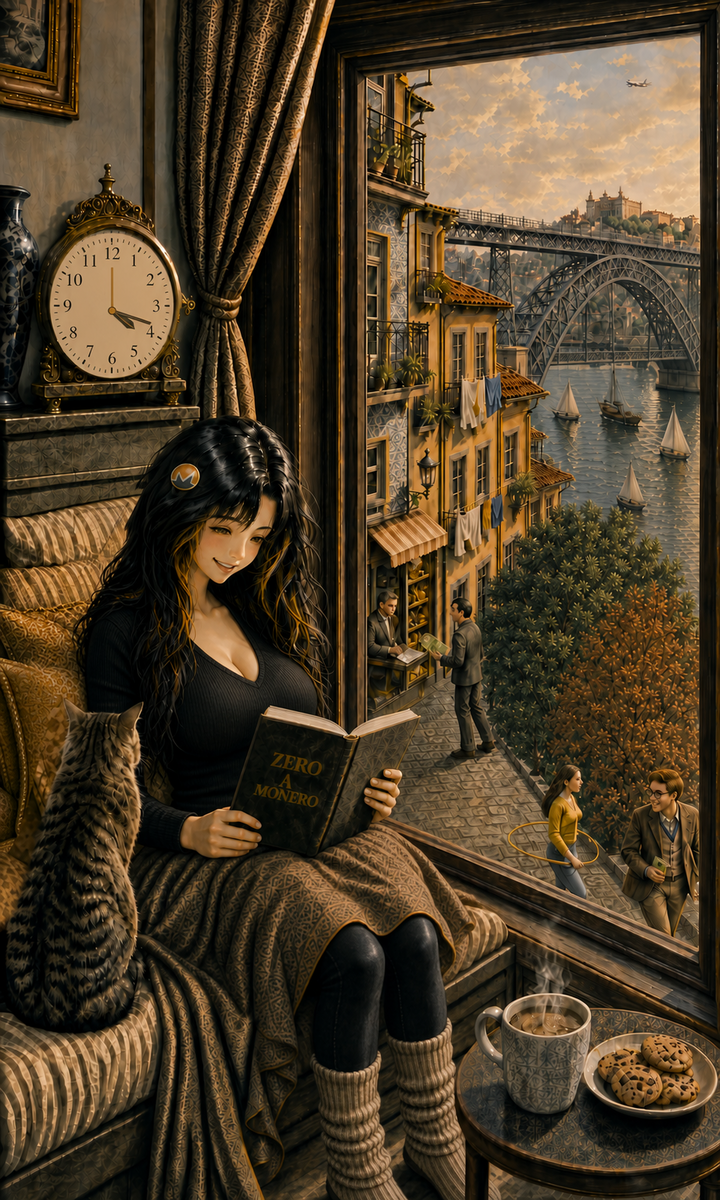
\includegraphics[width=\paperwidth,height=\paperheight]{front/figures/monerochan-autumn-porto-v11-final.png}%
    \hss
  }%
  \vss
}%
\endgroup


\end{document}
